\documentclass[11pt,a4paper]{article}
\usepackage[english]{babel}
\usepackage[utf8]{inputenc}
\usepackage[T1]{fontenc}
\usepackage{amsmath,amssymb}
\usepackage{booktabs}
\usepackage{longtable}
\usepackage{tabularx}
\usepackage{array}
\usepackage[numbers]{natbib}
\usepackage{hyperref}
\usepackage{enumitem}
\usepackage{algorithm}
\usepackage{algpseudocode}
\usepackage{geometry}
\usepackage{graphicx}
\usepackage{adjustbox}
\usepackage{float}
% Double rules at the top and bottom of every algorithm float.
\makeatletter
\newcommand\fs@dblrulled{%
  \def\@fs@cfont{\bfseries}\let\@fs@capt\floatc@ruled
  \def\@fs@pre{\hrule height 0.9pt depth 0pt\kern 1.2pt\hrule height 0.4pt depth 0pt\kern 2pt}%
  \def\@fs@post{\kern 2pt\hrule height 0.4pt depth 0pt\kern 1.2pt\hrule height 0.9pt depth 0pt\relax}%
  \def\@fs@mid{\kern 2pt\hrule\kern 2pt}%
  \let\@fs@iftopcapt\iftrue}
\makeatother
\floatstyle{dblrulled}
\restylefloat{algorithm}
%Includes "References" in the table of contents
\usepackage[nottoc]{tocbibind}

\geometry{margin=1in}
\hypersetup{colorlinks=true,linkcolor=blue,citecolor=blue,urlcolor=blue}

\newcommand{\fitfigure}[1]{\adjustbox{max width=0.98\linewidth,max totalheight=0.42\textheight,keepaspectratio}{#1}}

\title{Frankenstein Transformer:\\Unified Encoder-Decoder Library, CLI, and Research-Grounded Design Notes}
\author{
Erick F. Merino M. \\
This work is not affiliated \\
\texttt{erickfmm@gmail.com}
}
\date{October 2026}

\begin{document}

\maketitle

\begin{abstract}
Transformer architectures dominate sequence modeling across natural language processing, computer vision, and computational biology. Recent work has diversified attention beyond dense softmax---recurrent and retentive blocks, sparse patterns, gated mechanisms, latent projections, memory-augmented layers, and fast-weight rules---while optimizers have expanded beyond AdamW with variance-reduction, memory-efficient, schedule-free, second-order, and low-rank methods. Comparing these ideas under consistent conditions remains costly: each variant must be implemented, wired into a training pipeline, and maintained, which hinders reproducibility. We propose Frankenstein Transformer, a configuration-driven CLI toolkit (\texttt{frankenstein-transformer}) that unifies model definition, training, deployment, and inference behind one strict YAML schema. The toolkit covers forty-three sequence mixers across eight families and twenty-three optimizer families with per-parameter-group hyperparameter control, and supports encoder, decoder, and Vision Transformer model classes for masked language modeling, causal language modeling, sentence embeddings, and image tasks. The contribution of this software is a validated experimentation contract: invalid configurations fail before training, every architecture and optimizer shares one operational interface, and the same document drives training, quantized deployment and export, and a schema-generated web builder. We describe the architecture taxonomy, optimizer routing, deployment paths, and integration surface, and defer mathematical and implementation detail to the appendices.
\end{abstract}

\tableofcontents
\newpage

\section{Introduction}

\subsection{Motivation and Problem Statement}

Transformer architectures are the dominant paradigm for sequence modeling in natural language processing \citep{vaswani_attention_2017}, computer vision, and computational biology, with models such as BERT \citep{devlin_bert_2019} and GPT establishing the standard for representation learning. The field has since diversified rapidly: recurrent and retentive blocks, sparse attention, gated mechanisms, latent projections, memory-augmented layers, fast-weight rules, and continuous-depth formulations each address a different limitation of dense attention, while the optimizer landscape has expanded beyond AdamW with variance-reduction, memory-efficient, schedule-free, second-order, and low-rank methods \citep{child_sparse_transformer_2019,sun_retentive_2023,gu_mamba_2023,behrouz_titans_2025,ramapuram_theory_2024,xie_adan_2022,pagliardini_ademamix_2024,yuan_mars_2024,shazeer_adafactor_2018,zhao_galore_2024,defazio_road_2024,gupta_shampoo_2018,vyas_soap_2024}.

The practical consequence is a fragmented ecosystem. Comparing sequence mixers or optimizers under identical training conditions requires re-implementing each variant, wiring it into a training pipeline, and maintaining the result across framework changes. This effort hinders reproducibility, slows scientific progress, and raises the barrier to entry for new researchers.

\subsection{Proposal and Contributions}

We propose \textbf{Frankenstein Transformer} (\url{https://github.com/erickfmm/frankenstein-transformer}), a configuration-driven toolkit that treats architecture, optimizer, and training choices as a single validated document. The project provides:

\begin{enumerate}[leftmargin=*]
    \item \textbf{Schema-first design}: a strict YAML contract supporting forty-three sequence mixers across eight families and twenty-three optimizer families, enforced before training begins.
    \item \textbf{Architecture-agnostic training}: one pipeline for dense baselines, recurrent and retentive blocks, sparse patterns, gated mechanisms, latent compression, conditional memory, fast-weight attention, and geometric-field attention, with encoder and decoder modes \citep{zhu2026mixtureofdepthsattention,cheng2026conditionalmemoryscalablelookup,xie_mhc_2025,zhang_falcon_2026,pisoni_ssog_2026}.
    \item \textbf{Optimizer routing}: prefixed hyperparameter groups that control embeddings, normalization layers, attention blocks, and remaining parameters independently for each optimizer family \citep{zhu2025apollosgdlikememoryadamwlevel}.
    \item \textbf{End-to-end workflows}: training (including sentence-embedding objectives), deployment and export (quantized, standard, HuggingFace Transformers, and BitNet GGUF formats), inference, and a schema-driven web builder inspired by SBERT-style workflows \citep{reimers_sentence-bert_2019}.
    \item \textbf{Vision support}: a Vision Transformer model class covering masked patch prediction, classification, and segmentation under the same mixer and optimizer infrastructure.
    \item \textbf{Validation tooling}: unit tests, YAML preset validation, and continuous integration across supported Python versions.
\end{enumerate}

The command surface is \texttt{frankenstein-transformer}, with four subcommands: \texttt{train}, \texttt{deploy}, \texttt{infer}, and \texttt{web-server}. The last launches a Streamlit configuration builder that renders schema metadata as forms, validates input live, previews the resulting YAML, and generates the equivalent CLI command, serving both as a configuration aid and as documentation of the available design space.

\subsection{Reading Guide}

This document is organized as a technical reference:
\begin{enumerate}[leftmargin=*]
    \item \textbf{Prerequisites}: Appendix~\ref{sec:annex-tutorial} introduces transformers and attention for readers new to the field.
    \item \textbf{Configuration contract}: Section~\ref{sec:config-centric-architecture} describes the schema and Section~\ref{sec:schema-validation} its validation rules.
    \item \textbf{Architecture selection}: Section~\ref{sec:attention-families} compares sequence-mixer families; Appendices~\ref{sec:annex-transformer}, \ref{sec:annex-latent}, \ref{sec:annex-sparse}, and \ref{sec:annex-gated} collect the supporting literature, with normalization, BitNet, and conditional-memory details in Appendix~\ref{sec:annex-norm-bitnet-mod} and manifold-constrained residuals in Appendix~\ref{sec:annex-mhc}.
    \item \textbf{Optimization}: Section~\ref{sec:optimizer-families} summarizes optimizer routing; Appendix~\ref{sec:annex-optimizers} provides the full family analysis.
    \item \textbf{Deployment and inference}: Sections~\ref{sec:quantization} and~\ref{sec:sbert} cover quantized deployment and sentence embeddings.
\end{enumerate}

\section{Related Work}

This work sits at the intersection of deep learning frameworks, training tooling, and configuration-driven experimentation. While Sections~\ref{sec:attention-families} and~\ref{sec:optimizer-families} survey the architectural and optimization literature in depth, this section focuses on the software ecosystem for building, training, and configuring transformer models.

\subsection{Base Deep Learning Frameworks}

The modern transformer research ecosystem rests on several foundational frameworks that provide automatic differentiation, GPU acceleration, and high-level model-building APIs.

\textbf{PyTorch} \citep{paszke_pytorch_2019} has become the dominant framework for transformer research. Its imperative programming model and dynamic computation graphs enable flexible debugging and rapid prototyping of novel architectures. The \texttt{torch.nn.Module} abstraction, automatic mixed-precision training via \texttt{torch.cuda.amp}, and the \texttt{torch.compile} JIT compiler form the backbone of most contemporary transformer implementations. Frankenstein Transformer is built entirely on PyTorch, leveraging its module system for composable architecture definitions.

\textbf{TensorFlow} \citep{abadi_tensorflow_2016} pioneered production-oriented deep learning with its static computation graph paradigm and the Keras high-level API. While its influence in transformer research has waned relative to PyTorch, TensorFlow's serving infrastructure (\texttt{TF Serving}, \texttt{TF Lite}) and the \texttt{tensorflow-text} library remain relevant for deployment scenarios.

\textbf{JAX} \citep{bradbury_jax_2018} offers a functional programming model built around composable transformations (\texttt{jit}, \texttt{vmap}, \texttt{grad}) and XLA compilation. Its design enables clean implementations of complex algorithms and has been adopted by several recent transformer libraries (e.g., Flax, Haiku). JAX's stateless design and automatic vectorization are particularly well-suited for research on novel attention mechanisms and optimization algorithms.

\textbf{scikit-learn} \citep{pedregosa_scikit-learn_2011} provides classical machine learning algorithms and utilities (preprocessing, metrics, model selection) that serve as baselines and complementary tools in transformer workflows. While not designed for deep learning, its consistent API and extensive documentation make it a standard reference point for comparing transformer-based approaches against traditional methods.

\subsection{Out-of-the-Box Training Frameworks}

Several libraries provide complete training pipelines that abstract away the complexity of distributed training, data loading, and hyperparameter management.

\textbf{Hugging Face Transformers} \citep{wolf_huggingface_2020} is the de facto standard for accessing, fine-tuning, and sharing pretrained transformer models. Its \texttt{Trainer} API, model hub with over 500,000 models, and tight integration with the \texttt{datasets} and \texttt{tokenizers} libraries have made it the primary entry point for transformer-based NLP. However, its architecture is optimized for fine-tuning existing pretrained models rather than experimenting with novel sequence mixer designs or training from scratch with custom optimization strategies.

\textbf{Oumi} (\texttt{\url{https://github.com/oumi-ai/oumi}}, 2025) is an open-source end-to-end platform for training, fine-tuning, evaluating, and deploying foundation models. It provides a unified interface across multiple cloud providers and supports both supervised fine-tuning and preference optimization (DPO, RLHF). Oumi emphasizes production readiness with built-in monitoring, checkpointing, and deployment tooling.

\textbf{LLaMA Factory} (\texttt{\url{https://github.com/hiyouga/LLaMA-Factory}}, 2024) offers a unified framework for efficient fine-tuning of over 100 large language models. It provides both a web-based UI and a CLI, supporting LoRA, QLoRA, full-parameter fine-tuning, and various alignment techniques. Its focus is on adapting existing pretrained LLMs to downstream tasks rather than architectural experimentation.

\textbf{Axolotl} (\texttt{\url{https://github.com/axolotl-ai-cloud/axolotl}}, 2024) is a streamlined fine-tuning tool supporting LoRA, QLoRA, DeepSpeed, and FSDP. It emphasizes configuration-driven workflows via YAML files and has become popular in the open-source LLM fine-tuning community. Like LLaMA Factory, it targets fine-tuning of pretrained models rather than training novel architectures from scratch.

\subsection{Low-Code and Efficiency-Oriented Tools}

A growing category of tools prioritizes accessibility and computational efficiency, lowering the barrier to transformer training.

\textbf{Unsloth} (\texttt{\url{https://github.com/unslothai/unsloth}}, 2024) provides low-code fine-tuning with 2--5$\times$ speedup and significantly reduced VRAM requirements through hand-written CUDA kernels and optimized Triton operations. It supports GGUF export for quantized deployment and integrates with the Hugging Face ecosystem. Unsloth's focus is on making fine-tuning faster and more memory-efficient, not on architectural exploration.

\textbf{dashAI} (\texttt{\url{https://github.com/DashAISoftware/dashAI}}, v0.9.7.post2, 2026) is an open-source, local-first desktop workbench for machine learning developed by a Chilean academic consortium (Universidad de Chile/FCFM, CENIA, IMFD, and ANID funding). Its interface is fully schema-driven: configuration forms are generated directly from Pydantic component schemas with no hand-written frontend code, and its catalog spans roughly 76 multitask models---tabular classifiers, NLP models, translation, open-weight LLMs, and text-to-image generation---unified behind a dozen typed base abstractions. Extensibility is central to its design: plugins are ordinary PyPI packages discovered through the \texttt{dashai.plugins} entry-points group and installable from the UI, a mechanism comprehensive enough that even dashAI's own generative capabilities (e.g., Stable Diffusion, Flux) are distributed as plugins. Where earlier releases targeted classical ML workflows, the current platform spans predictive and generative modeling across domains, making it a natural host for transformer components via its plugin system; Section~\ref{sec:dashai-plugin} presents the \texttt{dashai-frankenstein} adapter built on this mechanism.

\subsection{Configuration-Driven Experimentation}

A common thread across the tools surveyed above is their focus on fine-tuning existing pretrained models. Hugging Face Transformers, LLaMA Factory, Axolotl, and Unsloth all assume a pretrained checkpoint as the starting point. Oumi supports training from scratch but targets standard architectures. None of these tools provide a systematic framework for experimenting with novel sequence mixer architectures, comparing diverse optimization algorithms under controlled conditions, or exploring the interaction between architectural choices and training dynamics.

\textbf{Frankenstein Transformer} fills this gap by providing a schema-first configuration system purpose-built for architecture experimentation. Its key differentiators include:

\begin{itemize}[leftmargin=*]
    \item \textbf{43 sequence mixers} spanning dense attention, recurrent/retentive blocks, sparse attention patterns, gated mechanisms, adaptive depth routing, and conditional memory layers, all selectable via a single YAML field.
    \item \textbf{23 optimizer families} with a prefixed hyperparameter routing system that enables per-parameter-group control across embeddings, normalization layers, attention blocks, and feed-forward networks.
    \item \textbf{Dual training modes} supporting both encoder-style masked language modeling (MLM) and decoder-style autoregressive (AR) next-token prediction, with specialized fine-tuning workflows for each.
    \item \textbf{Strict schema validation} via \texttt{additionalProperties: false} constraints that prevent configuration errors before training begins, ensuring reproducibility across experiments.
    \item \textbf{End-to-end workflows} spanning quantized deployment (ternary weight packing, INT8 activations) and sentence-embedding training inspired by SBERT \citep{reimers_sentence-bert_2019}.
    \item \textbf{Web-based configuration interface} providing schema-driven form rendering with inline documentation, real-time validation, and CLI command generation.
\end{itemize}

By decoupling architecture definition from training infrastructure through a validated configuration contract, Frankenstein Transformer enables systematic comparison of sequence mixer families and optimization strategies under identical training conditions---a capability not provided by any existing tool in the ecosystem.

\section{System Design and Architecture}
\label{sec:system-design}

\subsection{Configuration-Centric Architecture}
\label{sec:config-centric-architecture}

Experimentation in this project is \emph{schema first}. Rather than exposing loosely checked flags, model topology, optimizer family, training limits, and telemetry pass through a single validated configuration document, which reduces ambiguity when reproducing results and lets many architectures share one operational interface.

The authoritative contract is \texttt{src/schema.yaml}, a modular JSON Schema whose modules under \texttt{src/schema/} cover the model, model class, tokenizer, optimizer, SBERT, training, and dataset blocks. The top-level objects are \texttt{base\_model}, \texttt{tokenizer}, \texttt{model\_class}, \texttt{model}, \texttt{training}, \texttt{image}, \texttt{vision\_dataset}, and \texttt{text\_dataset}.

\paragraph{Model class.} The \texttt{model\_class} field selects among three variants:
\begin{itemize}[leftmargin=*]
    \item \textbf{\texttt{frankenstein}}: mixed-architecture encoder with the full range of sequence mixers, MoE, and advanced normalization, trained with masked language modeling.
    \item \textbf{\texttt{frankensteindecoder}}: autoregressive causal decoder for next-token generation; the runtime forces decoder masking.
    \item \textbf{\texttt{frankenstein\_vit}}: Vision Transformer over image patches for masked patch prediction, classification, and segmentation; the runtime forces encoder masking and the configuration requires the \texttt{image} and \texttt{vision\_dataset} blocks.
\end{itemize}

\paragraph{Training mode.} \texttt{model.dims.mode} controls masking: \texttt{encoder} uses bidirectional attention for masked language modeling, and \texttt{decoder} uses causal masking for autoregressive prediction.

\paragraph{Mixer selection.} \texttt{model.dims.layer\_pattern} is an ordered list of mixer identifiers drawn from the eight families described in Section~\ref{sec:architecture-taxonomy}; the schema fixes the accepted identifiers, and the complete enumeration appears in Figure~\ref{fig:comprehensive-taxonomy} and Appendix~\ref{sec:annex-summary-tables}.

\paragraph{Optimizer selection.} \texttt{training.optimizer.optimizer\_class} selects one of twenty-three optimizer families, summarized in Section~\ref{sec:optimizer-families} and detailed in Appendix~\ref{sec:annex-optimizers}.

\begin{figure}[t]
\centering
\fitfigure{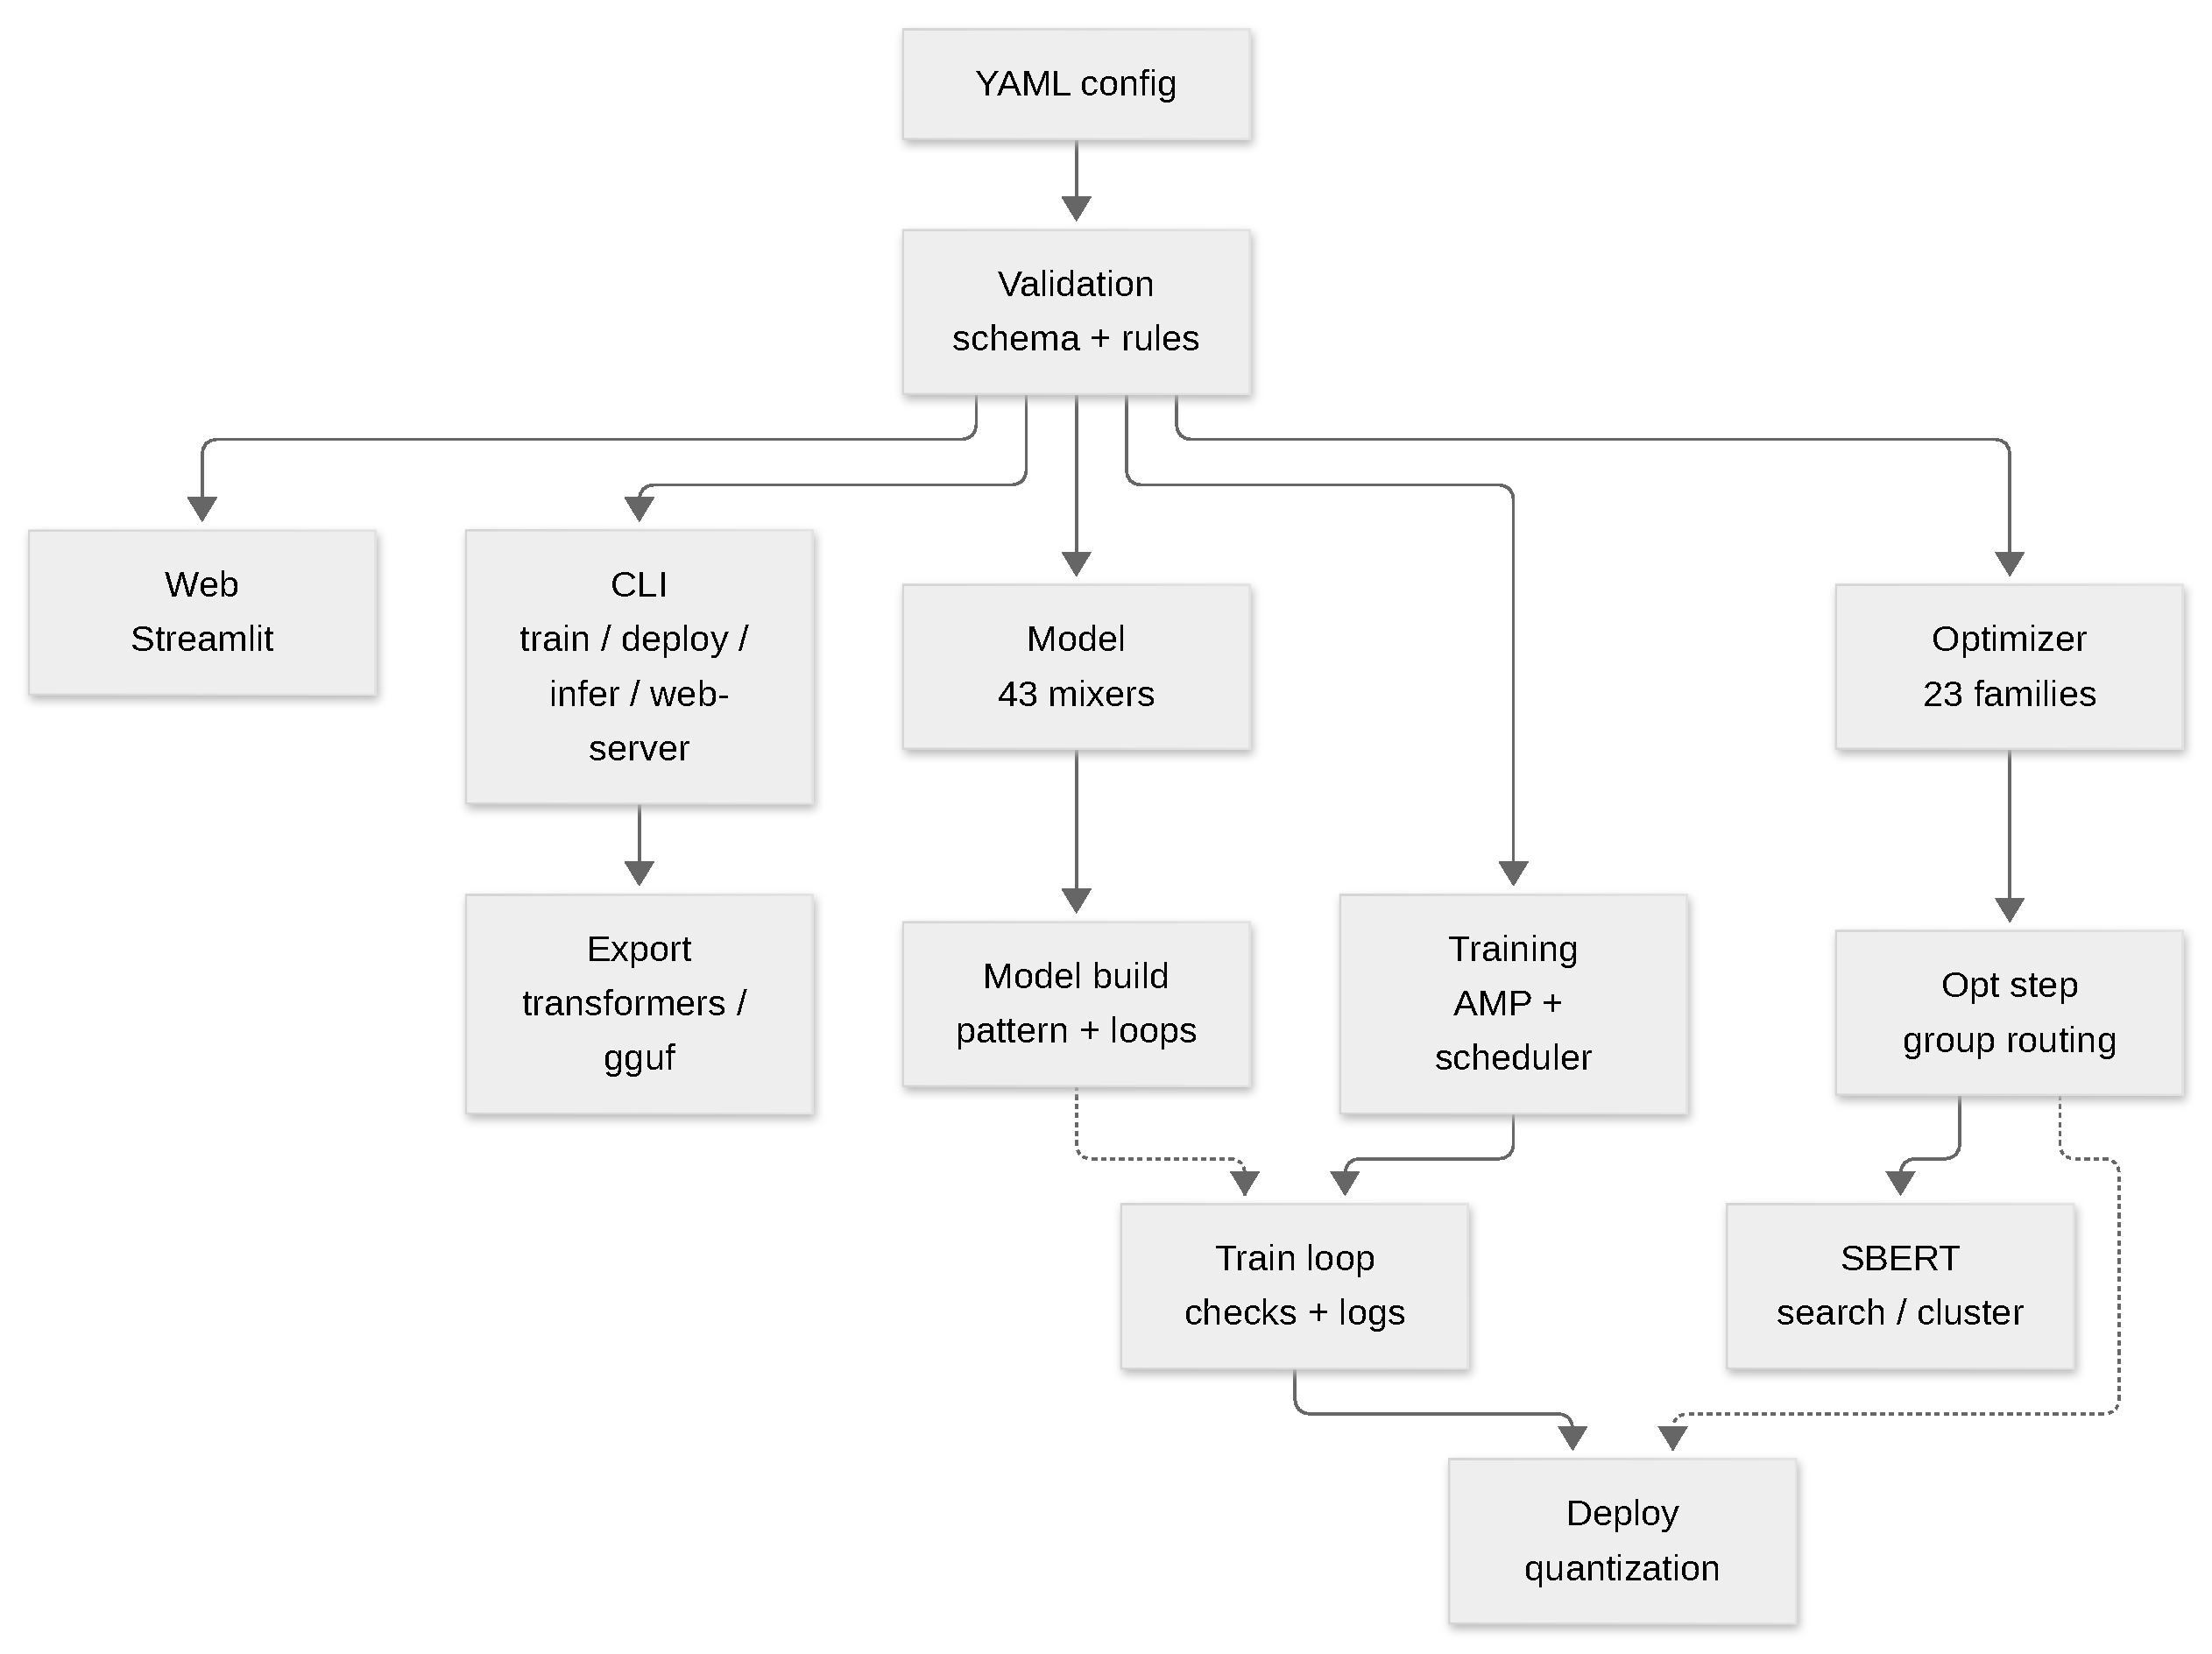
\includegraphics{figures/system-architecture.pdf}}
\caption{System architecture: configuration flows through validation, partitions into model, training, and optimizer components, executes at runtime, and produces deployment and SBERT artifacts.}
\label{fig:system-architecture}
\end{figure}

\subsection{Schema Scope and Validation Rules}
\label{sec:schema-validation}

Top-level and nested objects set \texttt{additionalProperties: false}, so unknown keys fail fast instead of being silently ignored. Optimizer parameters are further constrained by per-family prefix rules. Cross-component validation rejects incompatible combinations before training: hidden size must be divisible by the number of heads, the number of key--value heads must divide the number of heads, vocabulary size must match the tokenizer, a base model requires a task and (for MLM) a tokenizer, each task requires its matching optimizer block, BitNet router flags require BitNet to be enabled, and the decoder and vision classes force their respective masking modes.

\subsection{Configuration Schema}
The complete schema---fields, types, ranges, and validation rules---is documented in Appendix~\ref{sec:annex-schema}. Looped blocks are configured through \texttt{num\_layers} and \texttt{num\_loops}, giving \texttt{num\_layers}$\times$\texttt{num\_loops} logical layers at fixed parameter count.

\subsection{Training Tasks}

\texttt{training.task} selects the objective: \texttt{mlm} (masked language modeling), \texttt{causal\_lm} (autoregressive next-token prediction, decoder class only), \texttt{sbert} (sentence embeddings), \texttt{text\_classification} (encoder class only), and the vision tasks \texttt{patch\_prediction}, \texttt{classification}, and \texttt{segmentation} (Vision Transformer only). NLP tasks consume \texttt{text\_dataset}; vision tasks consume \texttt{vision\_dataset}. Sentence-embedding workflows are described in Section~\ref{sec:sbert}.

\subsection{Training Safety and Runtime Semantics}

The training step accumulates gradients over micro-batches, clips the global norm, checks for post-clip overflow, retries a bounded number of times on non-finite values, dispatches the configured scheduler, and rotates rolling and best checkpoints. The full pseudocode is deferred to Appendix~\ref{sec:annex-norm-bitnet-mod}.

\subsection{Normalization Variants}
\label{sec:normalization}

Normalization is both a modeling choice and a schema compatibility question. The accepted \texttt{norm.type} values are \texttt{layer\_norm}, \texttt{dynamic\_tanh}, \texttt{derf}, \texttt{rms\_norm}, \texttt{prms\_norm} (partial RMSNorm), and \texttt{flash\_norm} (weightless RMSNorm). Their formulations and comparison are detailed in Appendix~\ref{sec:annex-norm-bitnet-mod}.

\subsection{Residual-Stream Architectures}
\label{sec:residual-stream}

Residual connections are exposed as a macro-design choice through the \texttt{model.residuals} block:
\begin{itemize}[leftmargin=*]
    \item \textbf{Standard}: the classical identity residual \citep{he_deep_2016}.
    \item \textbf{None}: no skip connection, retained only as an ablation probe.
    \item \textbf{Attention Residuals} (\texttt{full\_attn} or \texttt{block\_attn}): learned attention over depth replaces the fixed residual sum, either over all previous layers or over block-wise summaries \citep{sun_attnres_2026}.
    \item \textbf{Manifold-constrained hyper-connections} (\texttt{mhc.enabled}): an $n$-stream residual whose mixing matrix is constrained to the Birkhoff polytope \citep{xie_mhc_2025}.
\end{itemize}

Attention Residuals compose with mHC and Mixture-of-Depths; the formulations, wiring, and reported results are collected in Appendices~\ref{sec:annex-attnres} and~\ref{sec:annex-mhc}.

\section{Architecture Taxonomy and Implementation}
\label{sec:architecture-taxonomy}

\subsection{Attention and Sequence-Mixer Families}
\label{sec:attention-families}

The system implements forty-four sequence mixers organized into eight functional categories that reflect how each method balances expressivity, computational cost, and memory.
\begin{enumerate}[leftmargin=*]
    \item \textbf{Dense baselines} (3): standard softmax attention, sigmoid attention, and Grouped-Query Attention (GQA) provide full global routing at quadratic cost.
    \item \textbf{Recurrent and retentive} (5): RetNet, Mamba, ODE-style blocks, and Titans maintain state for constant-time inference through recurrence, selective state spaces, continuous depth, or test-time memory.
    \item \textbf{Sparse patterns} (10): Sparse Transformer, Longformer, SWA with attention sinks, BigBird, SparseK, NSA, SpargeAttn, FASA, MSA, and SparDA reduce quadratic cost through structured sparsity, token selection, or training-free pruning.
    \item \textbf{Gated mechanisms} (8): GLA, DeltaNet, Gated DeltaNet, Gated DeltaNet-2, HGRN2, FoX, Gated Softmax, and KDA introduce data-dependent control over retention, forgetting, and update strength.
    \item \textbf{Latent compression} (10): MLA, GQLA, MLRA, Tucker, IHA, GTA, MTLA, CCA, CCGQA, and GMA compress key--value state into low-rank bottlenecks or route through a Gaussian-mixture latent memory.
    \item \textbf{Conditional memory} (1): Engram provides test-time read/write memory through learned lookups.
    \item \textbf{Fast-weight attention} (6): Falcon-1/2/3 and Falcon-1A/2A/3A treat the recurrent state transition as an online continual-learning rule \citep{zhang_falcon_2026}.
    \item \textbf{Geometric field} (1): SSOG applies a structured geometric prior over the attention matrix \citep{pisoni_ssog_2026}.
\end{enumerate}

\begin{figure}[t]
\centering
\fitfigure{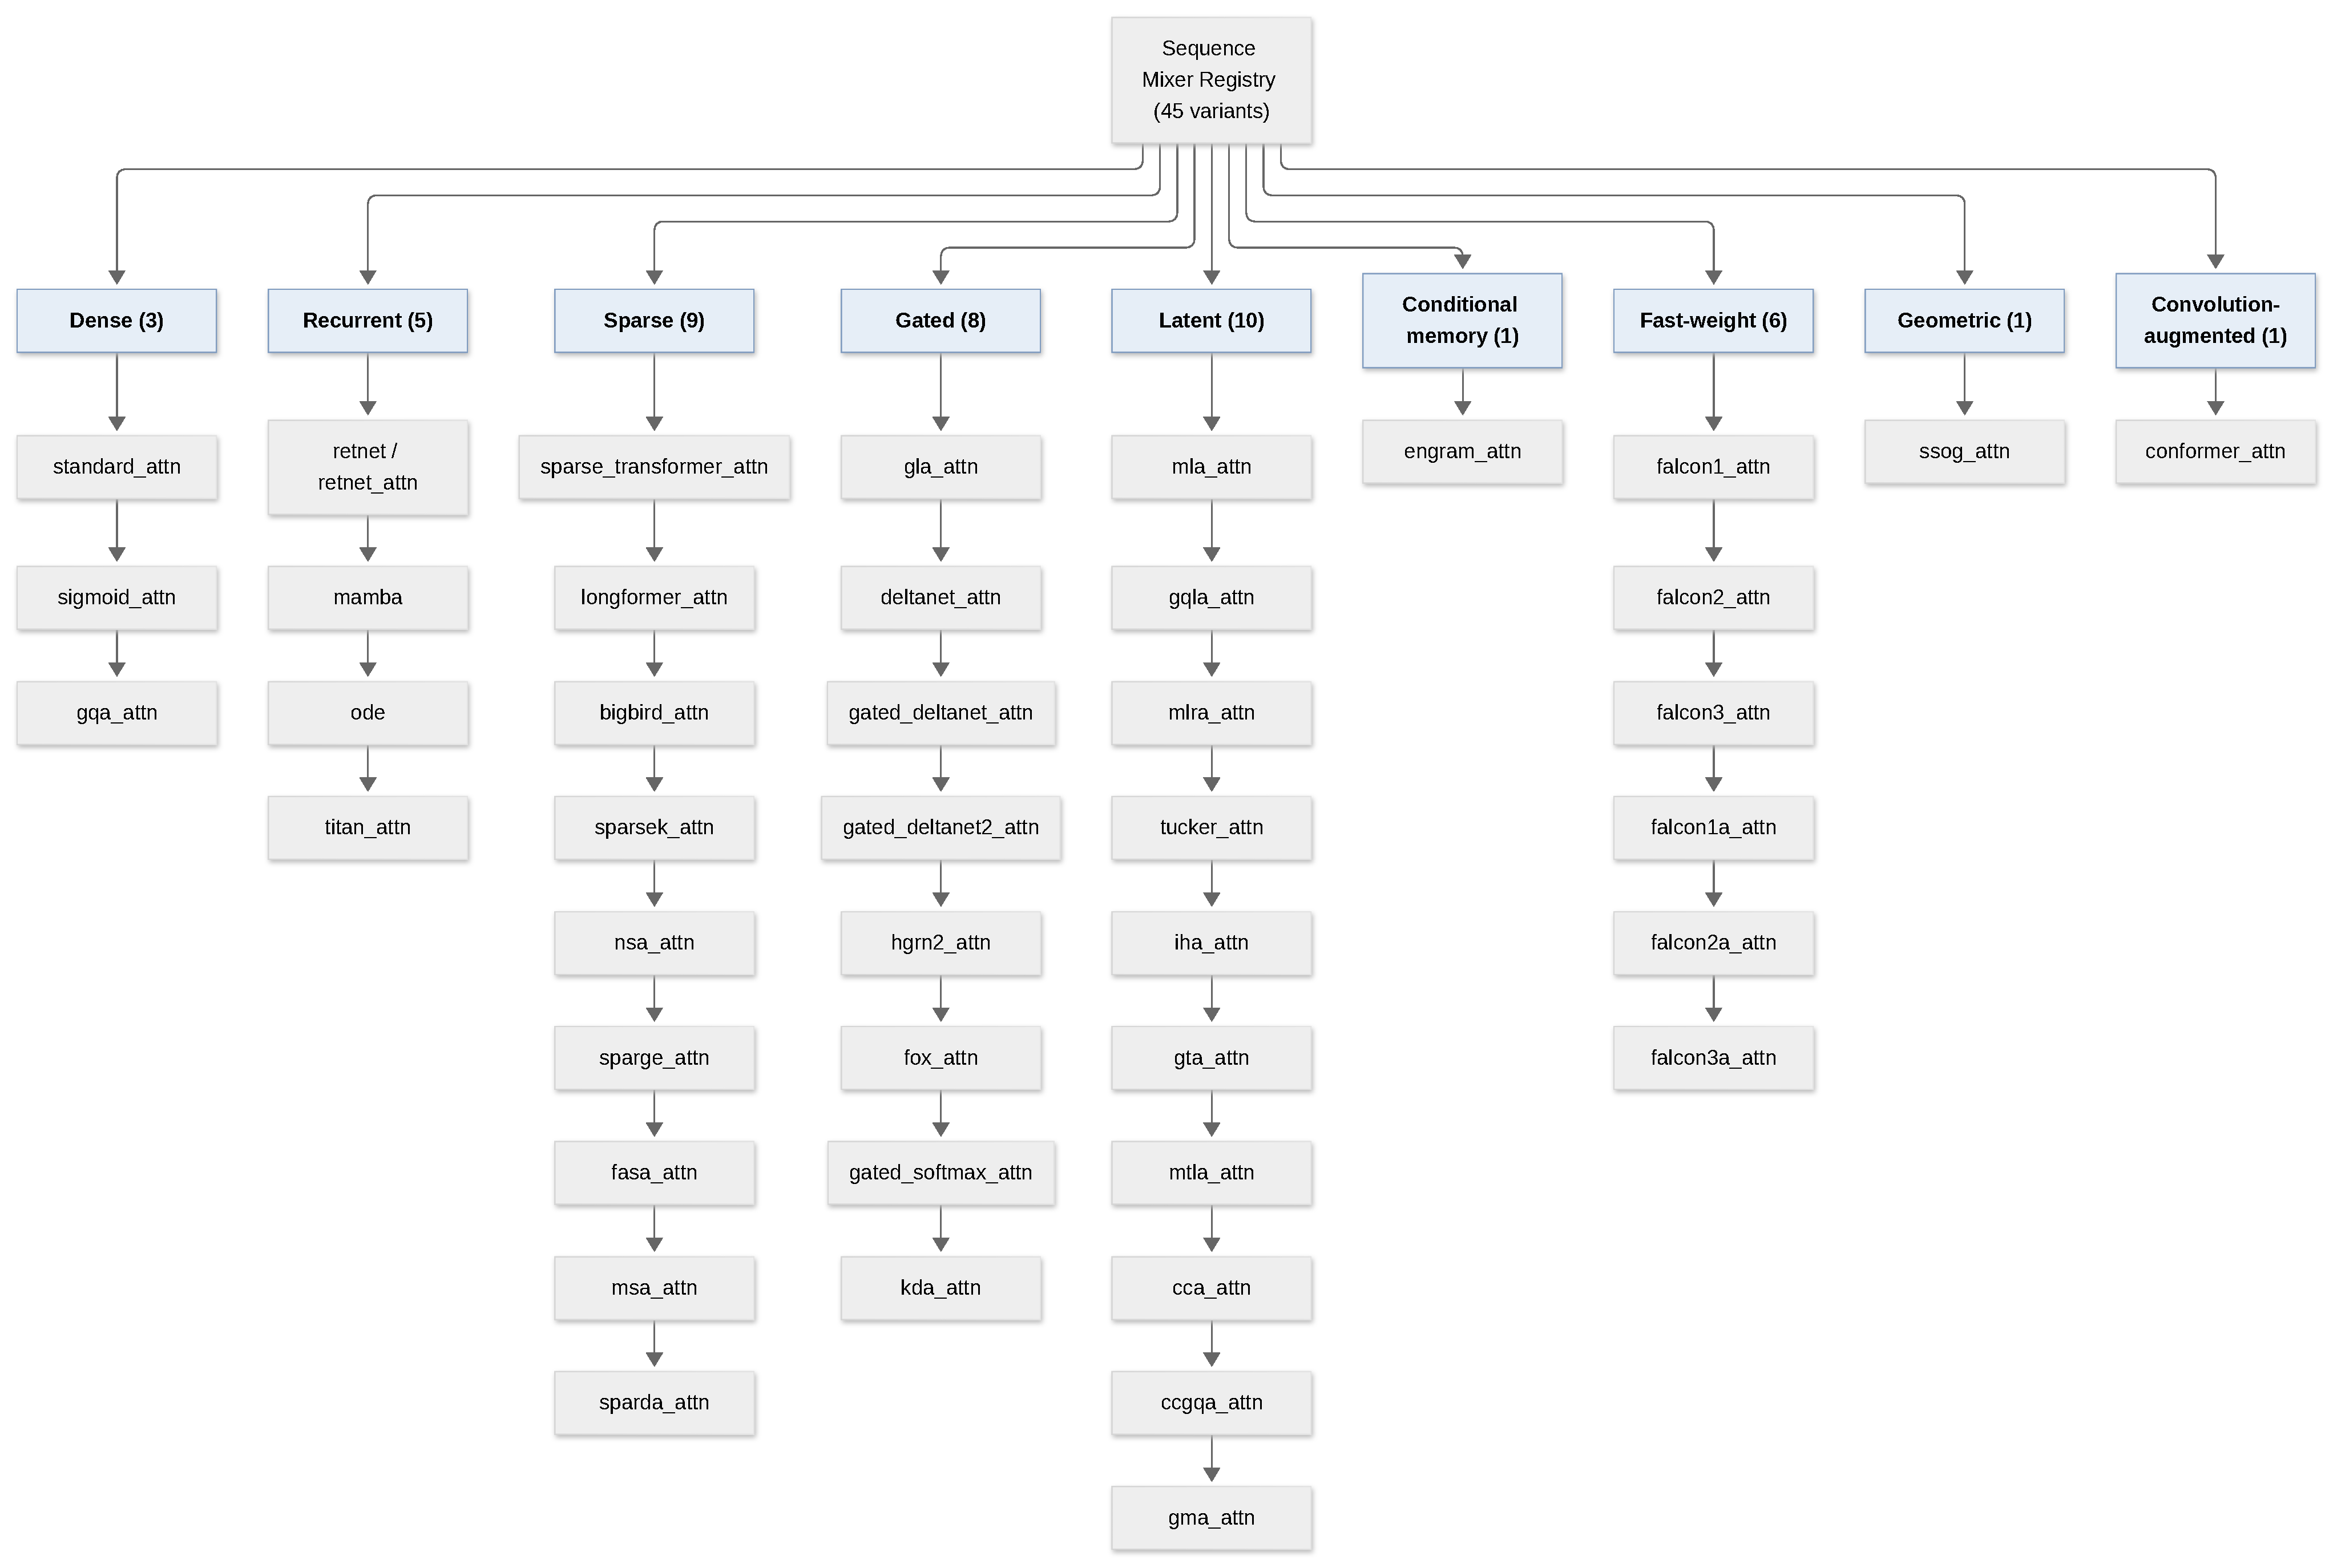
\includegraphics{figures/mixer-taxonomy.pdf}}
\caption{Taxonomy of the forty-three sequence mixers across eight functional categories. Dense baselines provide full global routing at quadratic cost; recurrent methods compress state for constant-time inference; sparse variants restrict the attention pattern; gated mechanisms modulate retention and forgetting; latent methods compress key--value representations; conditional memory adds test-time read/write lookups; fast-weight methods cast the state transition as an online learning rule; geometric methods encode structured priors.}
\label{fig:comprehensive-taxonomy}
\end{figure}

\subsection{Dense and Recurrent Families}
The dense baselines---standard softmax \citep{vaswani_attention_2017} and sigmoid attention \citep{ramapuram_theory_2024}---and the recurrent family---RetNet \citep{sun_retentive_2023}, Mamba \citep{gu_mamba_2023}, ODE-style blocks \citep{zhang_continuous_2021}, and Titans \citep{behrouz_titans_2025}---define the expressiveness-versus-efficiency trade-off. Formulations, parallel and recurrent forms, pseudocode, and a comparison table are collected in Appendix~\ref{sec:annex-transformer}.

\begin{figure}[t]
\centering
\fitfigure{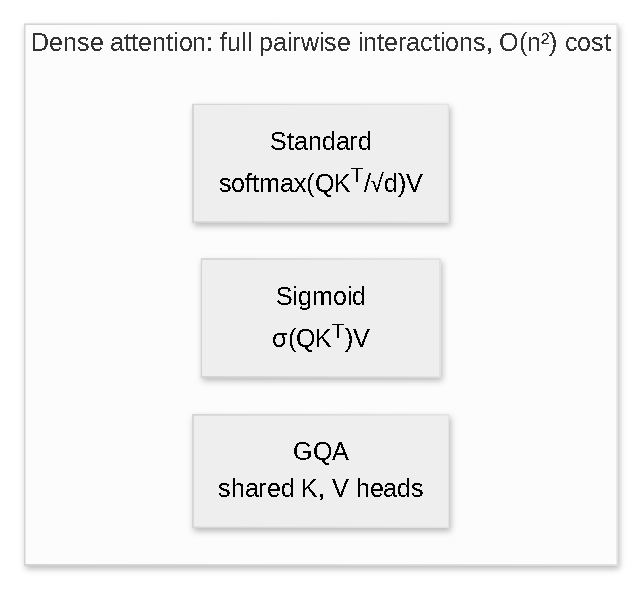
\includegraphics{figures/dense-map.pdf}}
\caption{Dense attention baselines. Standard and sigmoid attention compute full pairwise interactions; Grouped-Query Attention shares key--value heads across query groups, reducing memory traffic while keeping full attention expressivity.}
\label{fig:dense-map}
\end{figure}

\begin{figure}[t]
\centering
\fitfigure{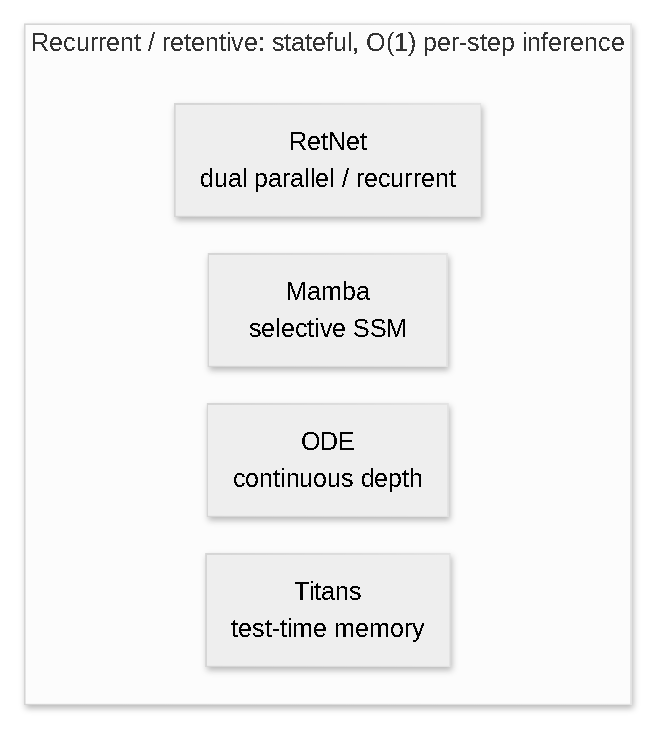
\includegraphics{figures/recurrent-map.pdf}}
\caption{Recurrent and retentive family. RetNet offers parallel and recurrent forms, Mamba uses selective state-space parameters, ODE blocks model continuous depth, and Titans add test-time memory; all achieve constant-time per-step inference.}
\label{fig:recurrent-map}
\end{figure}

\subsection{Latent and Low-Rank Attention Family}
This family compresses per-token key--value state into a low-rank latent: MLA, GQLA, MLRA, Tucker, IHA, GTA, and MTLA unify grouped-query, latent, factorized, and temporal designs. CCA and CCGQA formulate attention in a compressed latent with decoupled grouping, while GMA replaces pairwise interaction with probabilistic routing through learned Gaussian-mixture components. Formulations, pseudocode, and a comparison table are collected in Appendix~\ref{sec:annex-latent}.

\begin{figure}[t]
\centering
\fitfigure{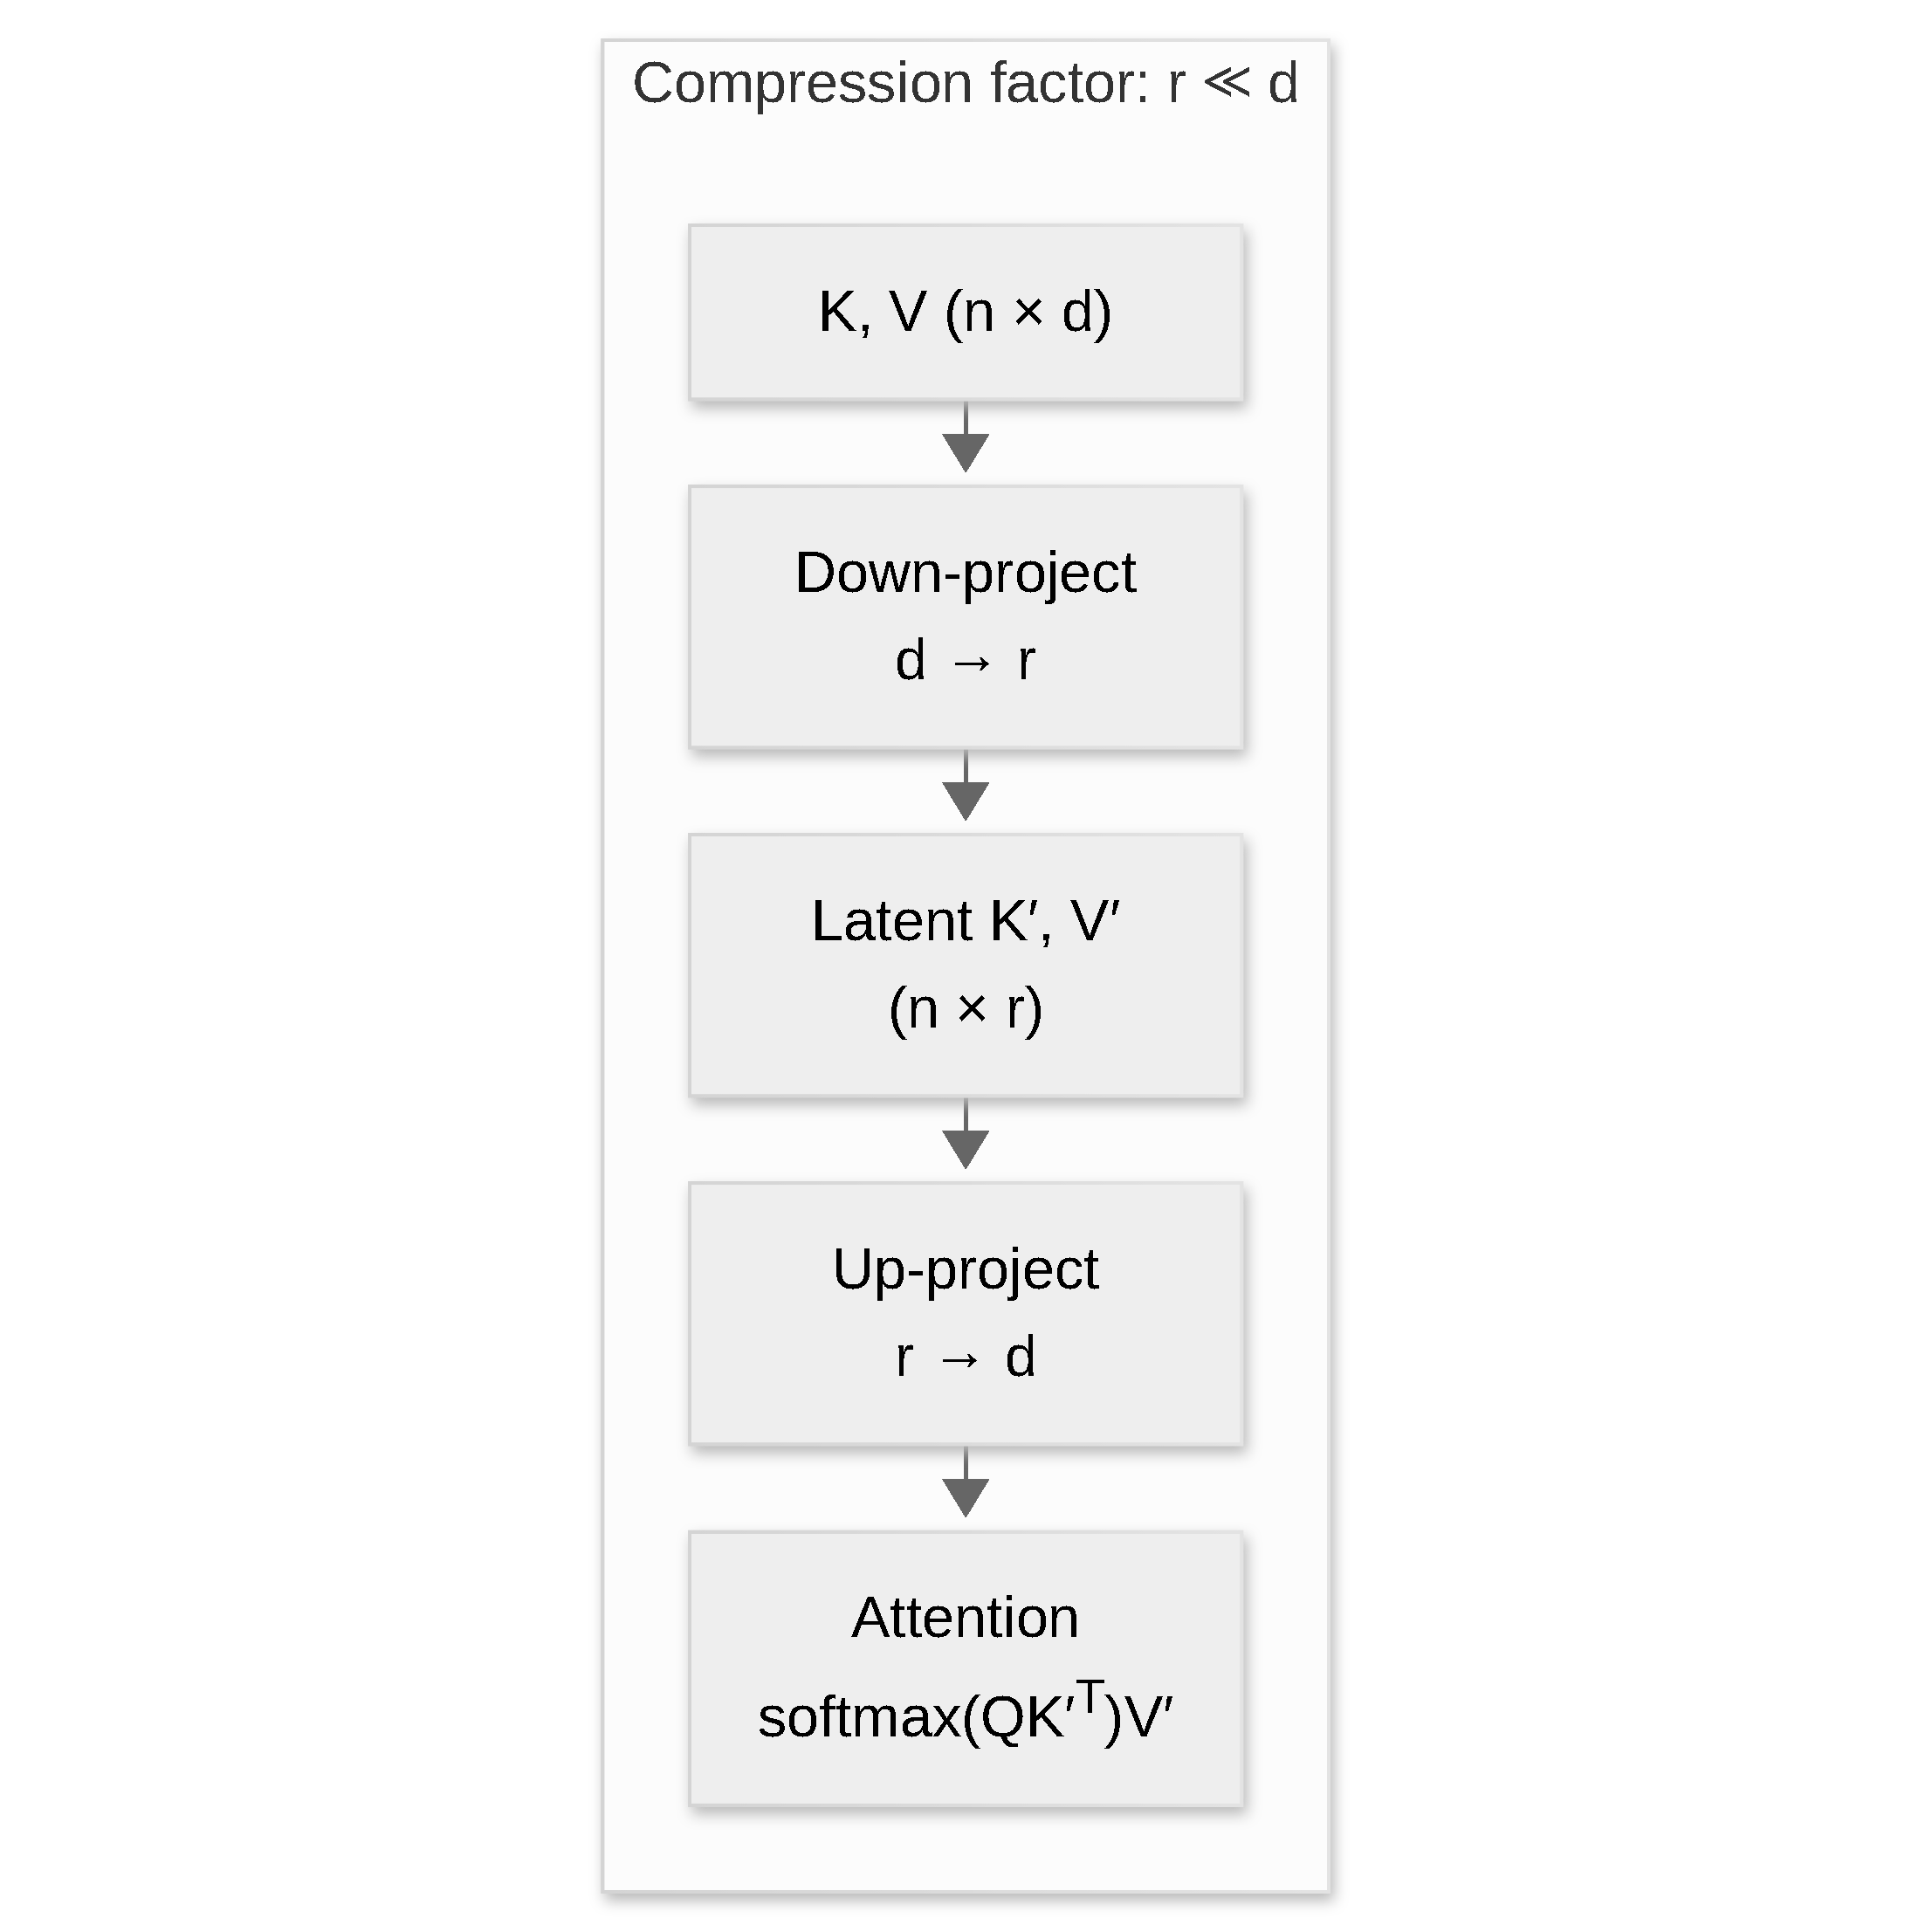
\includegraphics{figures/latent-map.pdf}}
\caption{Latent and low-rank attention. Key--value pairs are projected into a low-rank latent space, where attention is computed at reduced cost, and projected back. Variants differ in factorization, head interleaving, temporal compression, cross-covariance formulation, and probabilistic routing.}
\label{fig:latent-map}
\end{figure}

\subsection{Sparse Attention Extensions}
The registry includes ten sparse blocks \citep{child_sparse_transformer_2019,beltagy_longformer_2020,jolicoeur_sliding_window_2026,zaheer_bigbird_2020,lou_sparsek_2024,yuan_nsa_2025,zhang_spargeattn_2025,wang_fasa_2026,lai_minimax_2026,fu_sparda_2026}. Two inference-time methods, \texttt{fasa\_attn} and \texttt{sparge\_attn}, apply their sparse heuristic only when the model is in evaluation mode: during training the enclosing hybrid layer substitutes standard dense attention over the same $\mathbf{q}/\mathbf{k}/\mathbf{v}/\mathbf{o}$ projections, so the trained weights are exactly the ones the sparse path reads at inference. \texttt{swa\_attn} is also training-free but is a normal trainable mixer, so it runs its windowed pattern in both training and inference. Formulations, pseudocode, per-block characteristics, and a comparison table are collected in Appendix~\ref{sec:annex-sparse}.

\begin{figure}[t]
\centering
\fitfigure{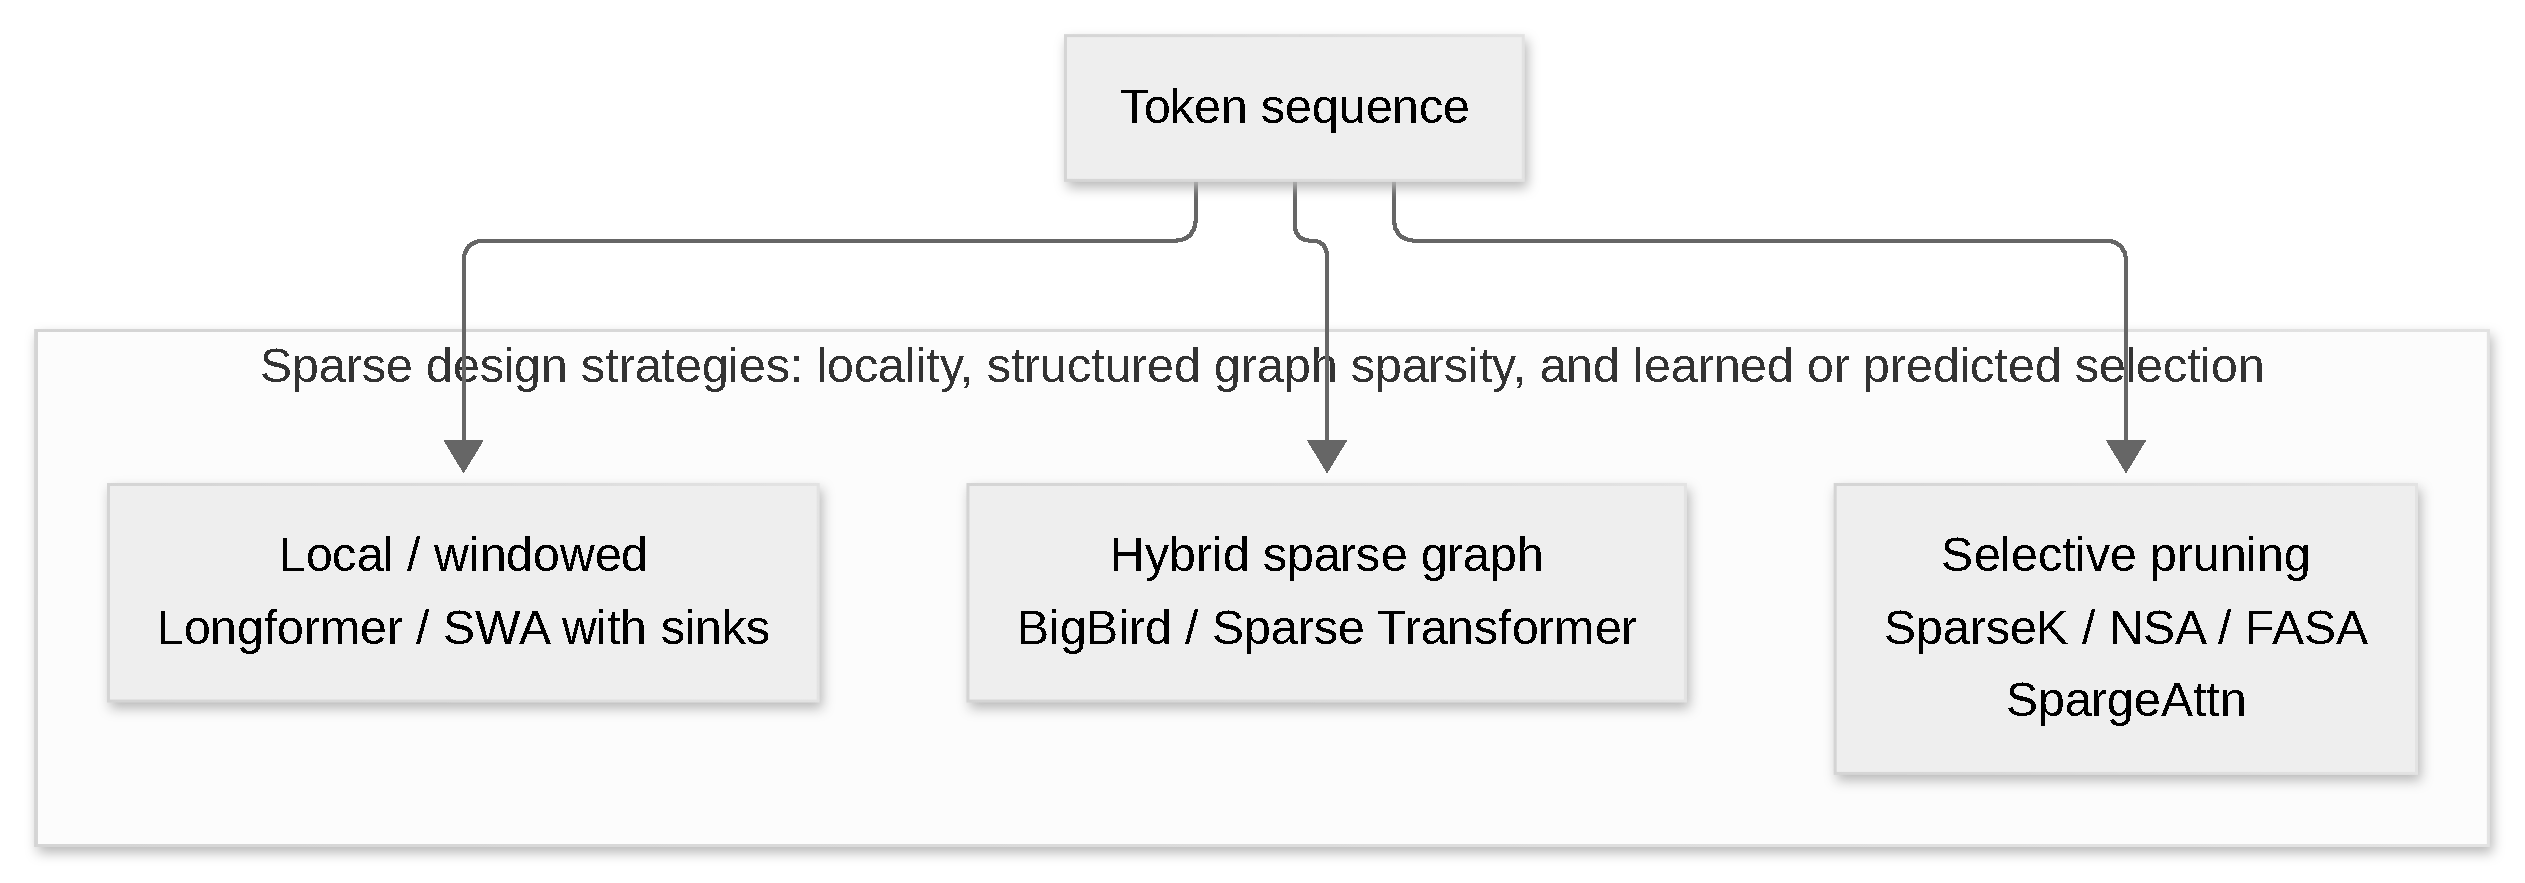
\includegraphics{figures/sparse-map.pdf}}
\caption{Sparse attention design choices. Methods reduce cost by restricting neighborhoods, constructing sparse graphs, or selecting only high-value tokens or blocks.}
\label{fig:sparse-map}
\end{figure}

\subsection{Gated and Fast-Weight Attention}
The gated family contains eight blocks \citep{yang_gla_2023,yang_deltanet_2024,yang_gated_deltanet_2024,hatamizadeh_gated_deltanet2_2026,qin_hgrn2_2024,lin_forgetting_transformer_2025,qiu_gated_attention_2025,kimi_kda_2025}. Gating controls what information survives, either in recurrent state updates (GLA, DeltaNet variants, HGRN2, KDA) or in the full attention path (FoX, Gated Softmax). Formulations, pseudocode, and a comparison table are collected in Appendix~\ref{sec:annex-gated}.

Fast-weight attention recasts the recurrent update as an online continual-learning rule; the six Falcon variants \citep{zhang_falcon_2026} unify DeltaNet-style regression and linear-attention writes under read-after-write semantics with normalized step sizes and explicit forgetting. Each variant ships a recurrent reference scan and a chunk-parallel kernel. Formulations, configuration knobs, and published results are collected in Appendix~\ref{sec:annex-fast-weight}.

\begin{figure}[t]
\centering
\fitfigure{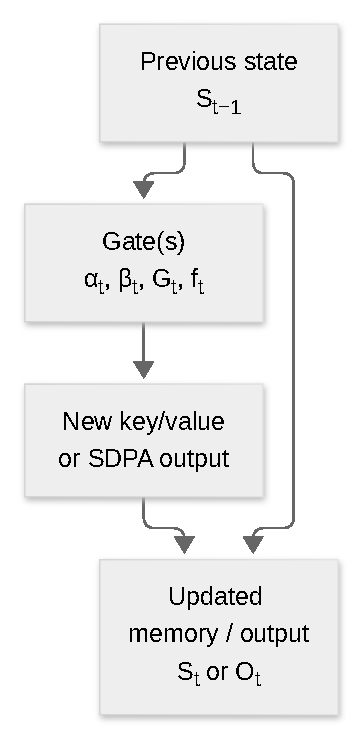
\includegraphics{figures/gating-template.pdf}}
\caption{Generic gating template. A gate can decay existing memory, regulate write strength, or modulate dense attention outputs, depending on the block family.}
\label{fig:gating-template}
\end{figure}

\section{Optimizer Families and Training Dynamics}
\label{sec:optimizer-families}

Optimizing large transformer architectures is complicated by non-convex landscapes, saddle points, and heterogeneous parameter groups. The system supports twenty-three optimizer families in seven categories: classical baselines (SGD with momentum, AdamW, RAdam); momentum and variance reduction (Adan, ADOPT, AdEMAMix, MARS, Cautious AdamW); memory-efficient and low-rank methods (Adafactor, GaLore, Lion, APOLLO, APOLLO-Mini, Q-APOLLO); schedule-free and parameter-free methods (Schedule-Free AdamW, Prodigy) with large-batch scaling (LAMB); curvature-aware and second-order methods (Sophia, Shampoo, SOAP); geometry-oriented methods (Muon, Turbo-Muon); and adaptivity-tunable optimizers (Anon). Algorithms, pseudocode, and memory and complexity comparisons are collected in Appendix~\ref{sec:annex-optimizers}.

\begin{figure}[t]
\centering
\fitfigure{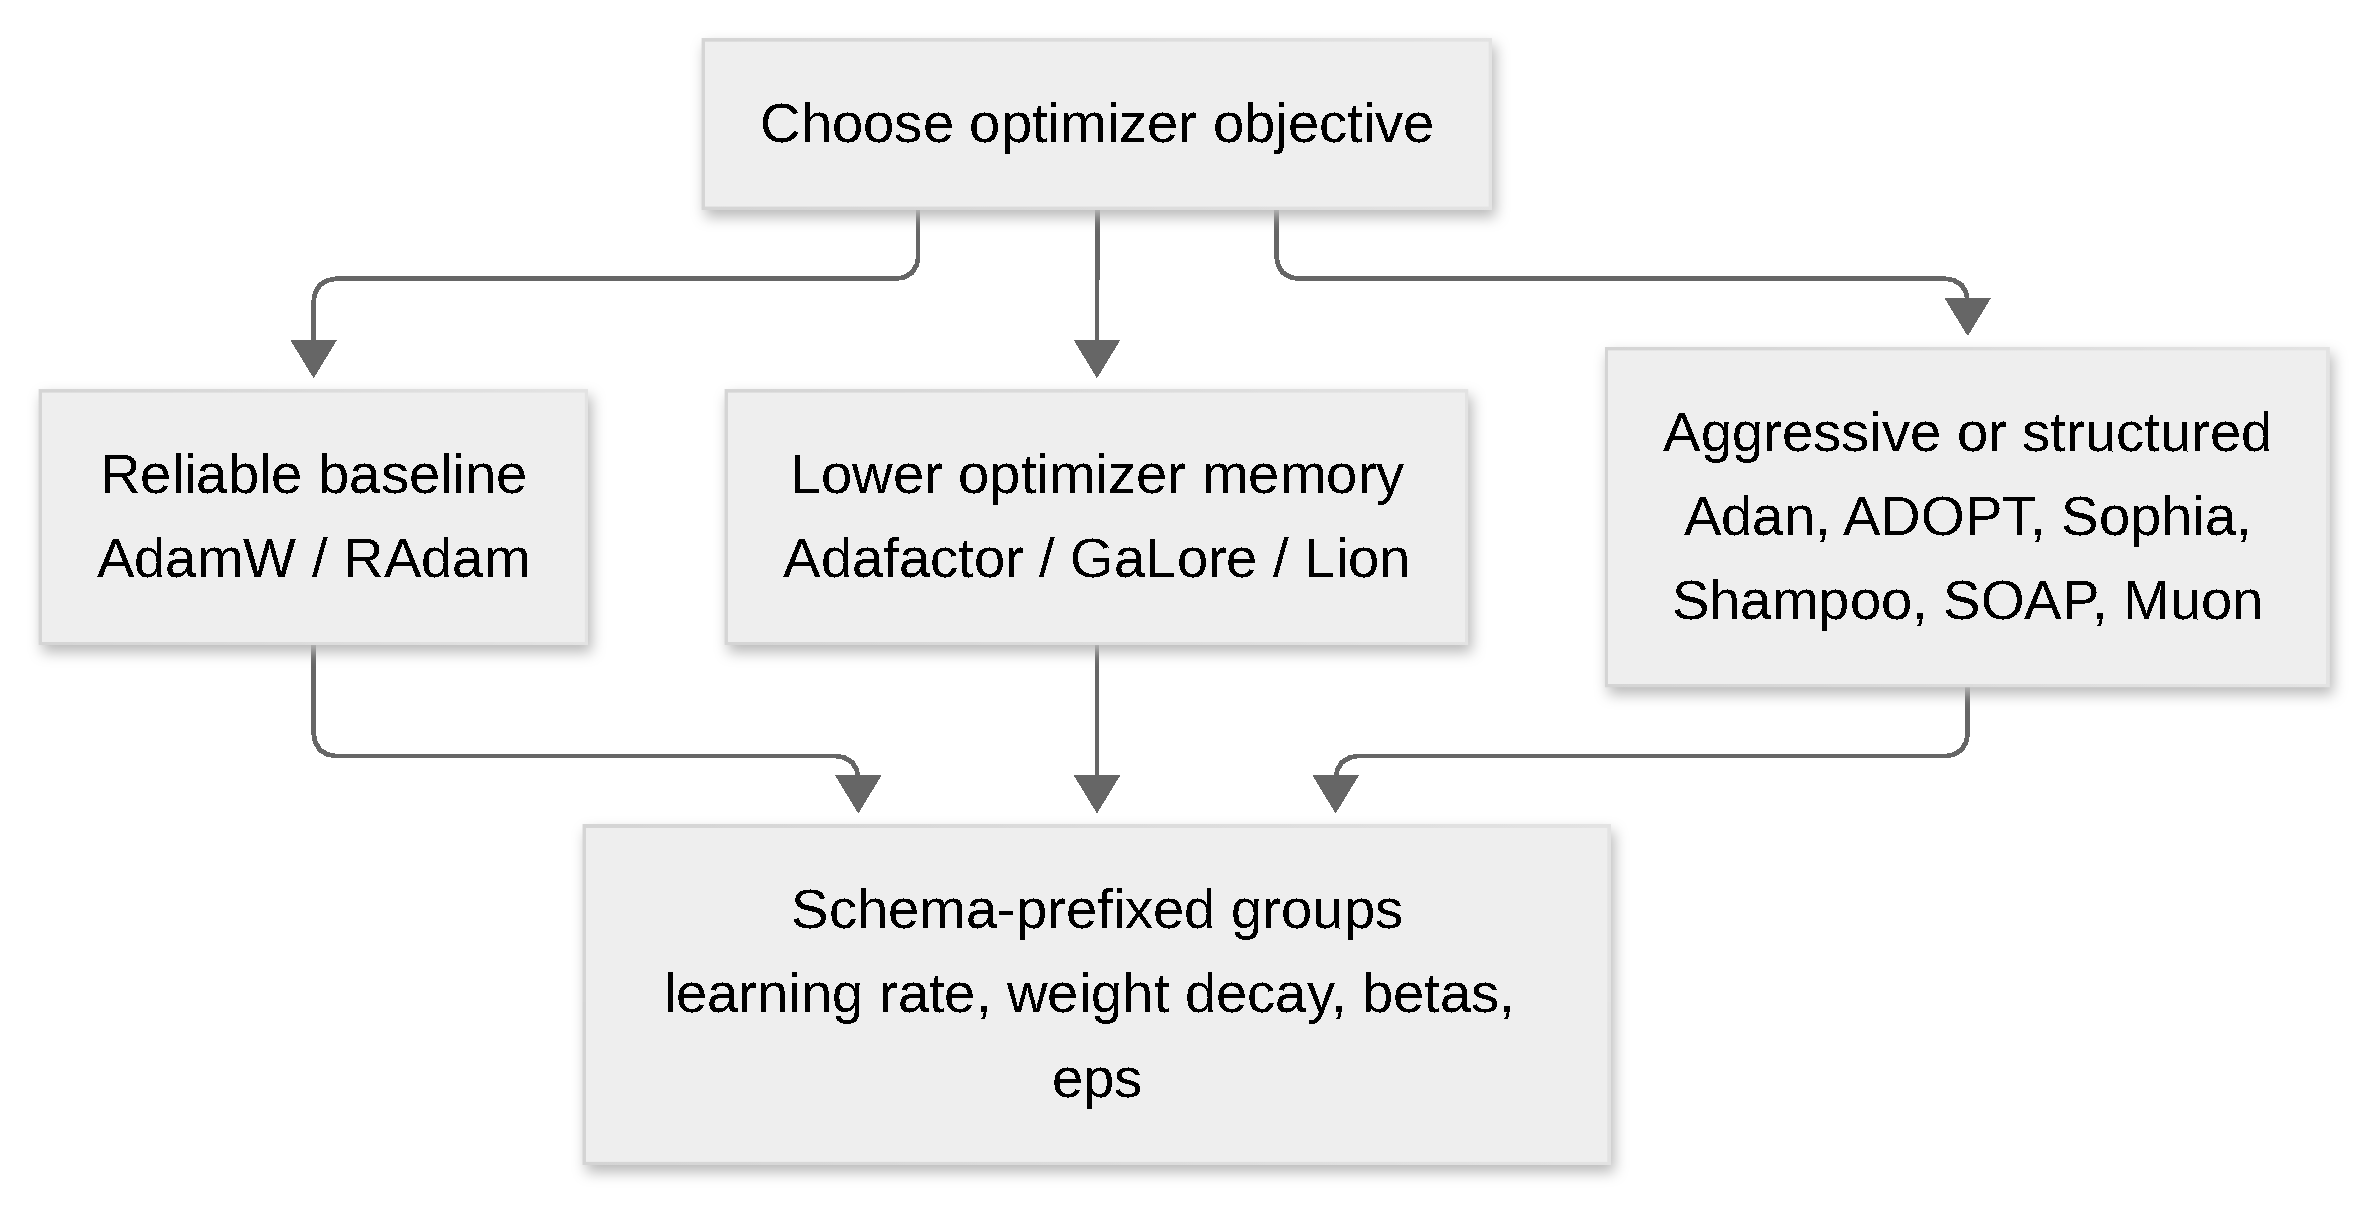
\includegraphics{figures/optimizer-routing.pdf}}
\caption{Optimizer selection in practice: the class determines the update rule, while the schema controls how hyperparameters apply across embeddings, normalization layers, attention blocks, and the remaining parameters.}
\label{fig:optimizer-routing}
\end{figure}

\section{Quantization and Deployment}
\label{sec:quantization}

The deploy stage converts a trained checkpoint into a compact artifact through ternary weight packing \citep{wang_bitnet_2023} and INT8 activation scaling, with size estimates aligned with lightweight deployment goals \citep{samson_lightweight_2026,bravin_embbert_2026}. The same subcommand emits standard or quantized artifacts, or exports HuggingFace Transformers and BitNet GGUF formats for external runtimes. The formulations and size estimates are deferred to Appendix~\ref{sec:annex-norm-bitnet-mod}.

\begin{figure}[t]
\centering
\fitfigure{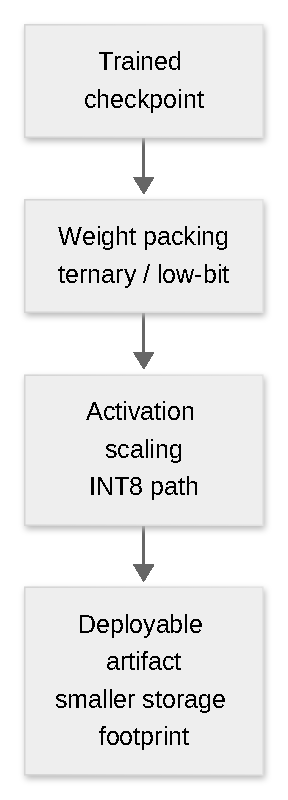
\includegraphics{figures/deploy-flow.pdf}}
\caption{Deployment path from a trained checkpoint to a compact artifact. Quantization is a deploy-stage transformation rather than a separate model family.}
\label{fig:deploy-flow}
\end{figure}

\section{SBERT Downstream Tasks}
\label{sec:sbert}

Sentence embedding is built on Siamese-style training \citep{reimers_sentence-bert_2019}. For sentence pair $(s_1,s_2)$ with embeddings $(e_1,e_2)$:
\[
\text{cos}(e_1,e_2)=\frac{e_1^\top e_2}{\|e_1\|\|e_2\|}
\]
and regression-style cosine loss:
\[
\mathcal{L}_{\text{cos}}=\left(\text{cos}(e_1,e_2)-y\right)^2
\]
with $y\in[-1,1]$ in this pipeline.

Supported downstream modes:
\begin{itemize}[leftmargin=*]
    \item \textbf{Similarity}: pairwise score between two sentences.
    \item \textbf{Search}: top-$k$ nearest neighbors over a corpus.
    \item \textbf{Cluster}: grouping embeddings (e.g., k-means).
    \item \textbf{Encode}: persistent embedding export for later retrieval.
\end{itemize}

\begin{figure}[t]
\centering
\fitfigure{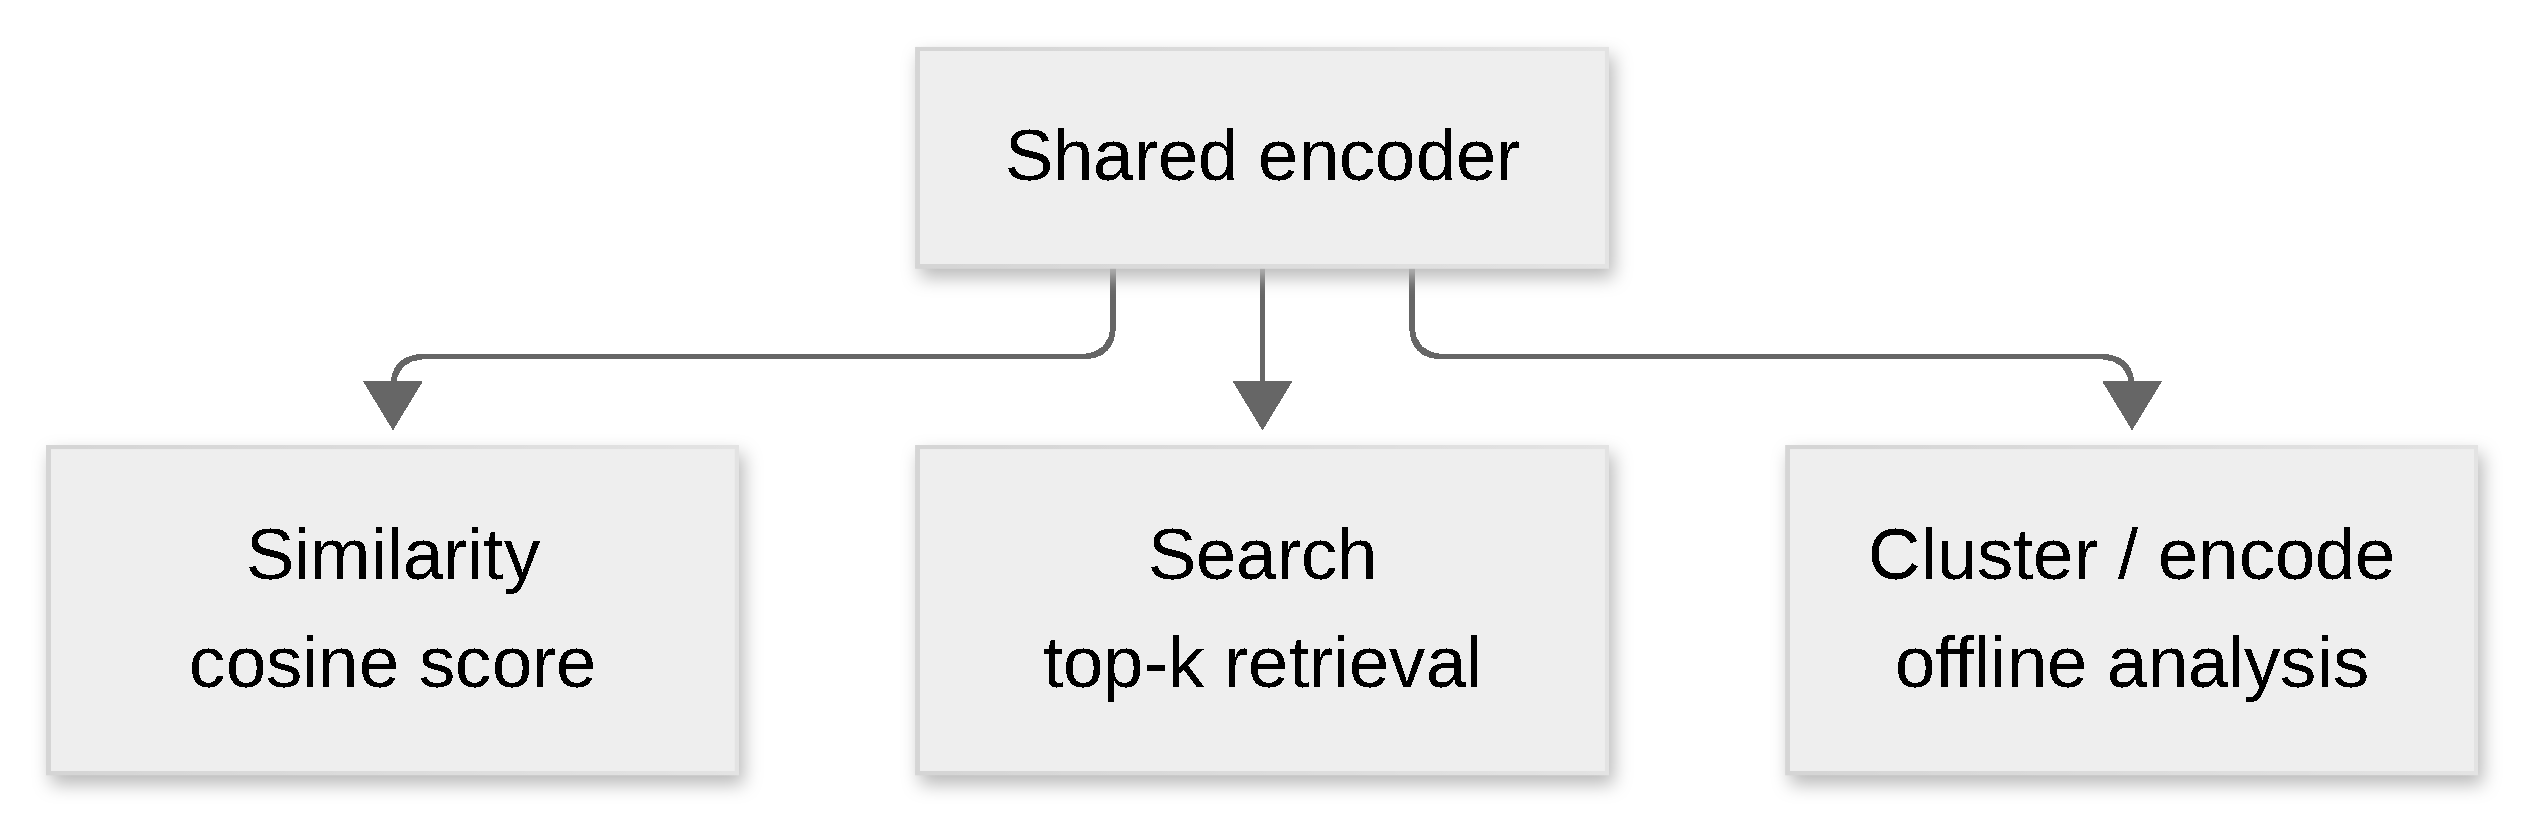
\includegraphics{figures/sbert-modes.pdf}}
\caption{SBERT workflow reuse. A single encoder supports online pair scoring, corpus retrieval, clustering, and persistent embedding export.}
\label{fig:sbert-modes}
\end{figure}

The pseudocode for the SBERT inference mode router---dispatching among similarity, search, cluster, and encode modes over a shared encoder---is deferred to Appendix~\ref{sec:annex-norm-bitnet-mod}.


\section{No-Code Integration: The \texttt{dashai-frankenstein} Plugin}
\label{sec:dashai-plugin}

The CLI and web builder described in Section~\ref{sec:system-design} serve researchers comfortable with YAML configuration files. A complementary audience---domain specialists, educators, and analysts who need a trained model but not a training script---is better served by a graphical environment. Frankenstein Transformer therefore ships \texttt{dashai-frankenstein}, an adapter that registers its model classes as components of \textbf{dashAI} (\texttt{\url{https://github.com/DashAISoftware/dashAI}}), an open-source, local-first machine-learning workbench developed by a Chilean academic consortium (Universidad de Chile/FCFM, CENIA, IMFD, and ANID funding). Both systems are schema-driven---dashAI renders forms from Pydantic schemas, Frankenstein validates YAML against a strict JSON Schema---so the integration leaves dashAI's backend untouched; the plugin is discovered through the standard \texttt{dashai.plugins} entry-points group documented in dashAI's plugin guide (\texttt{\url{https://docs.dash-ai.com/learn/guides/plugins/}}).

\subsection{Registered Components}

A single entry-points group registers five components:
\begin{itemize}[leftmargin=*]
    \item \textbf{\texttt{FrankensteinMLMModel}} (\texttt{BaseModel}, \texttt{TextClassificationTask}): encoder with a classification head over pooled output; \texttt{predict} returns per-class probabilities.
    \item \textbf{\texttt{FrankensteinDecoderModel}} (\texttt{BaseGenerativeModel}, \texttt{TextToTextGenerationTask}): forces the decoder class and exposes autoregressive top-$k$ sampling.
    \item \textbf{\texttt{FrankensteinViTClassifier}} (\texttt{BaseModel}, \texttt{ImageClassificationTask}): uses the ViT classification head (Appendix~\ref{sec:annex-vision}).
    \item \textbf{\texttt{FrankensteinViTSegmenter}} (\texttt{BaseModel}, plugin \texttt{SegmentationTask}): uses the ViT segmentation head and returns per-pixel class maps.
    \item \textbf{\texttt{SegmentationTask}} (\texttt{BaseTask}): declares the image-in/mask-out contract that dashAI does not ship.
\end{itemize}

All share one thin facade over the engine API, so the plugin has a single heavy dependency.

\subsection{Passthrough Configuration Schema}

The Frankenstein JSON Schema remains the single source of truth instead of translating its fields into native dashAI forms. Each component exposes one \texttt{frankenstein\_json} field holding a complete training configuration as single-line JSON. Before any training runs, the adapter parses the JSON, validates it against the resolved schema, and applies the config loader's cross-component checks; failures surface as a readable error tagged with the failing stage. Dataset adapters map dashAI datasets onto Frankenstein's expectations, inject the vocabulary size from the resolved tokenizer, and stream per-epoch metrics back to dashAI.

\subsection{Status}

The three implementation phases---classification MVP, generative decoder and ViT classifier, and ViT segmenter---are complete, but the package has not yet run inside a live dashAI instance and PyPI publication is pending. Known limitations include a direct classification loop rather than MLM pretraining, deferred native form fields for high-leverage knobs, and unconfirmed rendering of segmentation masks. The adapter deliberately leaves dashAI's core untouched, so future releases cannot break it through coupling.

\section{Discussion}
\label{sec:discussion}

The design choices in Frankenstein Transformer reflect several engineering and research tensions in modern deep learning tooling.

\subsection{Schema-Driven Design Trade-offs}

The schema-first approach provides significant reproducibility benefits by enforcing explicit contracts and failing fast on invalid configurations. However, this approach also introduces rigidity: adding new architectures or optimizers requires schema extensions rather than loose command-line arguments. The prefixed hyperparameter system enables fine-grained control but increases configuration complexity for users accustomed to simpler interfaces.

The decision to enforce \texttt{additionalProperties: false} at all schema levels eliminates silent parameter swallowing that has plagued earlier configuration systems, but this strictness requires careful schema maintenance when extending system capabilities. Each new attention mechanism or optimizer variant must be properly integrated into the validation framework, including schema field definitions with appropriate types and constraints, prefixed hyperparameter mapping for optimizer-specific groups, default values aligned with research best practices, and documentation strings for web interface rendering.

\subsection{Architectural Coverage and Gaps}

The forty-three implemented mixers span the major research directions in sequence modeling, but certain gaps remain. The system lacks recent hybrid architectures such as Griffin \citep{soares_griffin_2024} and Jamba \citep{gu_jamba_2024}, which combine gating with state-space models. MoE routing is implemented for FFN layers but not for attention computation, where recent work has shown benefits \citep{lewis_moe_2021}.

The sparse attention coverage is broad. The two inference-time methods (FASA, SpargeAttn) keep their training-free character in the sense that their sparsification rule is never learned; instead, the implementation trains the layer as standard dense attention over the same projections and activates the sparse selection/pruning path only at evaluation, so both mixers can be trained from scratch and their sparse behaviour is exactly the one described in the original papers.

The gated and fast-weight coverage spans the major categories, including the six Falcon variants \citep{zhang_falcon_2026}. Residual-stream macro-design is covered by Attention Residuals \citep{sun_attnres_2026} and by the manifold-constrained $n$-stream residual (mHC) \citep{xie_mhc_2025}, whose Sinkhorn--Knopp projection onto the Birkhoff polytope restores the identity-mapping property lost by unconstrained hyper-connections; mHC is validated only at the level of the published 3B--27B MoE experiments and would benefit from independent reproductions at smaller scales (Appendix~\ref{sec:annex-mhc}).

\subsection{Optimizer Landscape Fragmentation}

The support for twenty-four optimizer families across seven categories demonstrates comprehensiveness but also highlights the fragmented state of optimization research. Users face significant decision complexity when choosing among variance-reduction methods (Adan, MARS), memory-efficient variants (GaLore, Adafactor, APOLLO), and curvature-aware approaches (Sophia, Shampoo). The prefixed hyperparameter system, while powerful, requires understanding of which parameters are relevant for each optimizer class.

The implementation quality varies across optimizers: classical methods (AdamW, SGD with momentum) are highly optimized in PyTorch, while newer methods (Muon, Turbo-Muon, AF-Muon, SOAP) may require custom implementations that affect numerical stability and performance characteristics.

\subsection{Deployment and Production Considerations}

The quantization pipeline demonstrates practical deployment concerns but makes specific engineering trade-offs. Ternary weight packing reduces storage to approximately $1.58$ bits per parameter, but this aggressive compression may degrade performance, especially for smaller models where quantization error is more significant. The current implementation applies quantization uniformly across parameter types.

The SBERT workflows provide practical utility for semantic similarity and retrieval tasks, but implementation assumes standard pooling strategies (CLS token, mean pooling). Recent advances such as Matryoshka embeddings \citep{muennighoff_matryoshka_2021} and contrastive learning refinements \citep{chen_supervised_2020} are not yet incorporated.

\subsection{Integration and Extensibility Challenges}

The current codebase structure, while functional, presents maintenance challenges as architecture and optimizer families expand. The dispatcher pattern for mixer selection and optimizer routing handles extensibility but risks becoming a ``kitchen sink'' of conditional logic. Future versions would benefit from plugin-based architectures where new mixers and optimizers could be registered declaratively rather than modifying core dispatch logic.

The web configuration interface provides significant usability improvements but introduces deployment complexity: running Streamlit alongside training jobs requires additional resources and infrastructure considerations that may not be appropriate for all environments, particularly HPC clusters without web access.


\section{Conclusion}
\label{sec:conclusion}

Frankenstein Transformer presents a unified, configuration-driven experimentation platform addressing three challenges in modern deep learning research: architectural fragmentation across dense attention, recurrent models, sparse patterns, gated mechanisms, latent compression, conditional memory, fast-weight memories, and geometric priors; optimizer landscape complexity spanning classical baselines, variance-reduction methods, memory-efficient variants, schedule-free approaches, curvature-aware algorithms, and geometry-oriented methods; and end-to-end deployment workflows spanning quantization and sentence embedding.

The system's primary contributions are:
\begin{enumerate}[leftmargin=*]
    \item \textbf{Schema-First Design}: A strict YAML-based configuration contract with validation and prefixed hyperparameter routing enabling reproducible experiments across forty-three sequence mixers and twenty-three optimizer families.
    \item \textbf{Comprehensive Architecture Support}: Implementation spanning dense baselines, recurrent and retentive blocks, sparse attention, gated mechanisms, latent compression, conditional memory, fast-weight attention, and geometric-field attention, with encoder, decoder, and Vision Transformer model classes.
    \item \textbf{Unified Optimizer Framework}: Prefixed hyperparameter groups enabling fine-grained control over embeddings, normalization layers, attention weights, and the remaining parameters across classical baselines (SGD+Momentum, AdamW, RAdam), variance reduction (Adan, ADOPT, AdEMAMix, MARS, Cautious), memory-efficient and low-rank methods (Adafactor, GaLore, Lion, APOLLO, APOLLO-Mini, Q-APOLLO), large-batch and schedule simplification (LAMB, Schedule-Free AdamW, Prodigy), curvature-aware (Sophia), second-order (Shampoo, SOAP), geometry-oriented (Muon, Turbo-Muon), and adaptivity-tunable (Anon) optimizers.
    \item \textbf{End-to-End Workflows}: Integrated deployment pipeline supporting ternary weight packing and INT8 activation quantization; SBERT-inspired training and inference for semantic similarity, retrieval, and clustering tasks.
    \item \textbf{Interactive Configuration}: Streamlit-based web interface providing schema-driven form generation, real-time validation, inline documentation, and CLI command synthesis.
\end{enumerate}

This system enables rapid experimental iteration while maintaining reproducibility through strict configuration contracts. By consolidating diverse research contributions into a unified toolkit, it lowers barriers to exploring novel architectures and optimization strategies, particularly for researchers who may lack resources to implement and validate each variant independently.

\subsection{Limitations and Future Directions}

Several limitations and promising directions for future work emerge from this system's design and implementation:

\begin{enumerate}[leftmargin=*]
    \item \textbf{Architecture Integration}: Recent hybrid architectures (Griffin, Jamba, Mamba-X) demonstrate benefits of combining multiple mechanisms into unified blocks. Future versions should integrate these architectures and explore systematic composition patterns.
    
    \item \textbf{Advanced Quantization}: Current implementation uses uniform ternary packing across all parameters. Research on layer-wise, channel-wise, and importance-aware quantization suggests more sophisticated strategies could improve quality-efficiency trade-offs.
    
    \item \textbf{Plugin-Based Extensibility}: The current dispatch pattern becomes increasingly complex with each new addition. A plugin architecture allowing declarative registration of new mixers, optimizers, and normalization methods would improve maintainability and reduce risk of bugs in core dispatch logic.
    
    \item \textbf{Automated Hyperparameter Optimization}: The schema supports extensive hyperparameter spaces, but users must manually explore these spaces. Integration with Bayesian optimization, multi-armed bandit strategies, or gradient-based hyperparameter tuning could automate effective configuration discovery.
    
    \item \textbf{Production Deployment}: The web interface improves usability but may not be appropriate for all deployment environments. Headless configuration modes, API-based configuration management, or improved CLI ergonomics could serve HPC and production workflows.
    
    \item \textbf{Evaluation Benchmarking}: While the system enables training with diverse architectures, comprehensive benchmarking comparing performance across mixers and optimizers on standardized tasks would provide valuable guidance for configuration selection.
    
    \item \textbf{Training Stability Guarantees}: Current implementation includes NaN/Inf guards and gradient clipping, but formal analysis of stability conditions for different mixer-optimizer combinations, particularly with looped blocks and aggressive quantization, remains open.
    
    \item \textbf{Multimodal and Task-Specific Extensions}: The current design covers text and single-image tasks through the Vision Transformer class. Extensions to vision-language models, multimodal architectures, and task-specific fine-tuning workflows (e.g., instruction tuning, RLHF) would broaden applicability.
\end{enumerate}

The research trajectory of sequence modeling continues toward hybrid approaches that combine the strengths of multiple paradigms---compression from recurrence, selectivity from attention, gating for memory management, and sparsity for efficiency. A unified experimentation platform like Frankenstein Transformer becomes increasingly valuable as this convergence accelerates, enabling researchers to explore this expanding design space with reproducible, well-engineered infrastructure.



\bibliographystyle{plainnat}
\bibliography{../bibliography/other,../bibliography/optimizers,../bibliography/attention_types}

\appendix
\renewcommand{\thesection}{\arabic{section}}
\addtocontents{toc}{\bigskip\noindent\textbf{Appendices}\par}
\setcounter{section}{0}

\section{Conceptual Introduction---Transformers and Attention for Beginners}
\label{sec:annex-tutorial}

This appendix provides an accessible introduction to the fundamental concepts of transformers and the attention mechanism, aimed at readers without deep prior knowledge in deep learning. Transformers are the engine behind modern artificial intelligence systems like ChatGPT, but their operation can be understood through real-world analogies.

\subsection{What is a Transformer?}

A transformer is a neural architecture that processes text or data sequences by interpreting the meaning of each word while considering all other words in context. Imagine you read a sentence:

\begin{center}
\textit{``The bank was full of people waiting. Mary went to the bank.''}
\end{center}

What does ``bank'' mean in each case? In the first sentence, it refers to a financial institution (or a bench). In the second, it is less clear without context. A transformer solves this automatically by looking at all surrounding words. In the second sentence, seeing ``Mary went'', the model better understands that it probably is a riverbank (where she goes to swim) or a financial institution (where she goes to conduct a transaction).

This ability to understand the complete meaning of a word by considering the entire sentence is called \emph{contextualization}, and it is the heart of how modern transformers work.

\subsection{The Attention Mechanism: An Analogy}

The attention mechanism is the ``magic trick'' that allows transformers to understand context. Think of it as participating in an important conversation in a noisy room:

\begin{enumerate}[leftmargin=*]
    \item \textbf{Lots of noise}: Someone is speaking and being very important to you.
    \item \textbf{You ignore the rest}: Your brain automatically focuses attention on that person, ignoring other sounds.
    \item \textbf{You understand better}: By concentrating, you catch every word clearly.
\end{enumerate}

The neural attention mechanism works the same way: each word ``asks'' how important every other word is to understanding its meaning, then ``focuses'' its attention on the most relevant ones.

\subsection{Practical Example Step-by-Step}

Let's see how a transformer understands the word ``eats'' in two different contexts:

\subsubsection{Context 1: ``The cat eats fish''}

The transformer, when processing ``eats'', internally asks:
\begin{itemize}[leftmargin=*]
    \item How relevant is ``The''? Little (it's just an article). \textbf{Low attention}.
    \item How relevant is ``cat''? Very relevant (it's the subject, who eats). \textbf{High attention}.
    \item How relevant is ``fish''? Very relevant (it's what is eaten). \textbf{High attention}.
\end{itemize}

Thus, the mental representation of ``eats'' focuses primarily on ``cat'' and ``fish''.

\subsubsection{Context 2: ``The restaurant eats into profit margins''}

Here the transformer asks in a different context:
\begin{itemize}[leftmargin=*]
    \item How relevant is ``restaurant''? Very relevant (it's the subject). \textbf{High attention}.
    \item How relevant is ``profit''? Very relevant (it's affected). \textbf{High attention}.
    \item How relevant is ``margins''? Very relevant (it's what's being consumed). \textbf{High attention}.
\end{itemize}

The word ``eats'' gets a completely different representation because it ``attends'' to different words in different contexts.

\subsection{How Attention Works Mathematically (Simple Version)}

Behind the attention shift is mathematics. Here is the simplified version without too much technical detail:

\subsubsection{Step 1: Queries, Keys, and Values}

Each word in the sentence is transformed into three versions:
\begin{itemize}[leftmargin=*]
    \item \textbf{Query}: ``What information do I need to know?''
    \item \textbf{Key}: ``What information do I have?''
    \item \textbf{Value}: ``Here is my important information.''
\end{itemize}

Imagine in a library, each visitor is a ``query'', each book is a ``key'', and the content is the ``value''. The librarian (attention) matches queries with the most relevant keys to access the correct value.

\subsubsection{Step 2: Compatibility}

The system examines how \emph{compatible} each query is with each key. Queries similar to keys get a \emph{high} compatibility score. This is calculated by multiplying the query by the key (mathematically, the dot product).

\subsubsection{Step 3: Focus}

The compatibility scores are converted into ``focus weights''. High compatibilities mean ``focus attention here'', and low ones mean ``ignore this''. Mathematically, a function called \texttt{softmax} converts scores into percentages (like: 40\% attention here, 35\% here, 25\% there).

\subsubsection{Step 4: Combine}

Finally, the system combines all values, weighted by the focus weights. If a word has 80\% attention on the subject, 80\% of the subject's information gets blended into that word's representation.

\subsection{Multiple Attention Heads: Multiple Perspectives}

A key feature is that transformers do not use a single attention but \emph{multiple attention heads} in parallel. It's as if you had 8 people analyzing the sentence \emph{simultaneously}, each paying attention to different aspects:

\begin{itemize}[leftmargin=*]
    \item \textbf{Person 1}: ``I focus on subject-verb relationships.''
    \item \textbf{Person 2}: ``I search for the direct object.''
    \item \textbf{Person 3}: ``I track information about verb tense.''
    \item \textbf{Person 4}: ``I search for modifiers and adjectives.''
\end{itemize}

Each ``head'' learns to focus on different language patterns. Together, they capture much richer understanding than a single head.

\subsection{Stacking Layers}

Transformers process information in \emph{multiple layers} (usually 12 to 48 for practical models). Imagine editing an essay:
\begin{enumerate}[leftmargin=*]
    \item \textbf{First pass}: You fix spelling and basic grammar.
    \item \textbf{Second pass}: You improve clarity and sentence structure.
    \item \textbf{Third pass}: You ensure consistency and narrative flow.
\end{enumerate}

Transformers work the same way: each layer refines text understanding. The first layer captures basic features (simple words, genders), while later layers understand complex concepts (word relationships, abstract meanings).

\subsection{Why Does It Matter?}

The attention mechanism was revolutionary because:
\begin{enumerate}[leftmargin=*]
    \item \textbf{Parallelism}: It finds context for \emph{any word with any other word}, without processing them sequentially (unlike earlier systems). This makes it very fast.
    \item \textbf{Flexibility}: It learns what patterns to look for automatically from data, without you needing to program rules manually.
    \item \textbf{Scalability}: It works from small texts to contexts with millions of words.
    \item \textbf{General Capabilities}: The same mechanism works for translation, summarization, question-answering, text generation, computer vision, and more.
\end{enumerate}

\subsection{Practical Challenges}

Despite the extraordinary success of transformers, they present challenges:

\subsubsection{Computational Complexity}

If a sentence has 1,000 words, the standard attention mechanism must compare each word with all other 1,000 words. That's $1,000 \times 1,000 = 1,000,000$ comparisons. For long documents with millions of words, this becomes prohibitively expensive in time and memory.

\subsubsection{Memory Requirements}

Especially during inference (when using trained models), storing the entire attention matrix can consume enormous amounts of RAM or GPU memory, limiting the sequence lengths you can process.

\subsubsection{Device Efficiency}

Transformers were designed for powerful TPUs and GPUs. Running them on phones or embedded devices is challenging.

\subsection{Modern Solutions}

To solve these challenges, research has proposed many variants:

\begin{itemize}[leftmargin=*]
    \item \textbf{Sparse Attention}: Instead of comparing each word with ALL others, it compares only with a strategic subset (nearby neighbors, periodic patterns). Reduces complexity from $\mathcal{O}(n^2)$ to $\mathcal{O}(n \log n)$ or $\mathcal{O}(n)$.
    \item \textbf{Recurrent Models}: Like Mamba, they incorporate aspects of old recurrent neural networks but with better modern efficiency.
    \item \textbf{Gated Attention}: Mechanisms that selectively learn what information to pass forward, reducing storage needs.
    \item \textbf{Quantization}: Use smaller numbers (integers instead of decimals) to reduce memory without losing too much precision.
\end{itemize}

These innovations are what this toolkit (Frankenstein) allows you to experiment with easily.

\subsection{Key Takeaways}

\begin{itemize}[leftmargin=*]
    \item A \textbf{transformer} is a neural network that understands language context very well.
    \item The \textbf{attention mechanism} allows each word to ``focus'' on which other words are relevant to understanding its meaning.
    \item Attention works by computing \textbf{compatibility} between each word (query) and all others (keys), then combining information based on that compatibility (values).
    \item \textbf{Multiple heads} of attention explore different patterns in parallel.
    \item \textbf{Multiple layers} progressively refine understanding.
    \item The main challenge is that standard attention has quadratic complexity, which is expensive for long texts.
    \item Many \textbf{modern solutions} (sparse attention, recurrent models, quantization) address these challenges, and this toolkit lets you explore all of them.
\end{itemize}


\section{Configuration Schema Structure}
\label{sec:annex-schema}

The Frankenstein Transformer toolkit enforces a strict YAML configuration schema with \texttt{additionalProperties: false} at all levels. The schema is defined in \path{src/schema.yaml}, which references modular sub-schemas in \path{src/schema/}. Every configurable field must be declared in the schema; unrecognized keys are rejected at validation time. This appendix documents the complete schema structure, including all fields, their types, constraints, and cross-component validation rules.

\subsection{Top-Level Structure}

The root schema object has the following top-level properties. All are optional except \texttt{training}, which is required:

\begin{itemize}[nosep]
    \item \texttt{base\_model} (string) --- HuggingFace model identifier or local path for continual pretraining or SBERT fine-tuning. When set, \texttt{model\_class} and \texttt{model} are not required (the architecture is inferred from the checkpoint).
    \item \texttt{tokenizer} (object) --- Tokenizer configuration, available to both the \texttt{base\_model} path and custom from-scratch models. Two modes are selected via \texttt{source}: \texttt{hf\_repo} (default) loads a pretrained tokenizer from \texttt{name\_or\_path}; \texttt{train\_from\_dataset} trains a new tokenizer from the dataset text (see \S\ref{subsec:tokenizer-config}). Required when using \texttt{base\_model} with the \texttt{mlm} task.
    \item \texttt{model\_class} (enum) --- Model architecture variant: \texttt{frankenstein\_text\_encoder} (mixed-architecture encoder), \texttt{frankenstein\_text\_decoder} (autoregressive causal decoder), or \texttt{frankenstein\_vit} (vision transformer). Required when \texttt{base\_model} is not set.
    \item \texttt{model} (object) --- Model architecture parameters (see \S\ref{subsec:model-config}). Required when \texttt{base\_model} is not set.
    \item \texttt{training} (object, \textbf{required}) --- Training configuration (see \S\ref{subsec:training-config}).
\end{itemize}

The schema enforces a mutual-exclusivity rule: either \texttt{base\_model} must be present, or both \texttt{model\_class} and \texttt{model} must be present.

\subsection{Model Configuration}
\label{subsec:model-config}

The \texttt{model} object defines all architectural hyperparameters. Required fields are \texttt{dims.vocab\_size}, \texttt{dims.hidden\_size}, \texttt{dims.num\_layers}, \texttt{dims.num\_heads}, and \texttt{dims.layer\_pattern}. Table~\ref{tab:model-fields} lists all model fields with their types and descriptions.

\begin{longtable}{>{\ttfamily\footnotesize\raggedright\arraybackslash}p{5.6cm}>{\raggedright\arraybackslash}p{2.4cm}>{\raggedright\arraybackslash}p{6.9cm}}
\toprule
\textbf{Field} & \textbf{Type} & \textbf{Description} \\
\midrule
\endfirsthead
\toprule
\textbf{Field} & \textbf{Type} & \textbf{Description} \\
\midrule
\endhead
\midrule
\multicolumn{3}{r}{\textit{continued on next page}} \\
\endfoot
\bottomrule
\caption{Complete model configuration fields. All fields are optional unless marked required.}
\label{tab:model-fields}
\endlastfoot
\midrule
\multicolumn{3}{l}{\textit{model.dims.*}} \\
\midrule
dims.mode & enum (encoder, decoder) & Attention masking mode. \texttt{encoder} = bidirectional; \texttt{decoder} = causal. \\
dims.vocab\_size & int $\ge 1$ (required) & Number of unique tokens in the vocabulary. Must match the tokenizer's vocab size. \\
dims.hidden\_size & int $\ge 1$ (required) & Hidden dimension. Must be divisible by \texttt{num\_heads}. Typical: 512--2048. \\
dims.num\_layers & int $\ge 1$ (required) & Number of physical transformer layers. Typical: 6--24. \\
dims.num\_loops & int $\ge 1$ & Logical loop count. Each layer in \texttt{layer\_pattern} runs \texttt{num\_loops} times. Default: 1. \\
dims.num\_heads & int $\ge 1$ (required) & Number of parallel attention heads. Must divide \texttt{hidden\_size} evenly. \\
dims.dropout & float [0,1] & Global dropout rate. Typical: 0.1 (BERT standard). \\
dims.layer\_pattern & array of enum (required) & Ordered sequence of layer types. Length must equal \texttt{num\_layers}. 43 mixer codes available (see Table~\ref{tab:layer-pattern}). \\
\midrule
\multicolumn{3}{l}{\textit{model.norm.*}} \\
\midrule
norm.type & enum & Normalization strategy: \texttt{layer\_norm}, \texttt{dynamic\_tanh}, \texttt{derf}, \texttt{rms\_norm}, \texttt{prms\_norm}, \texttt{flash\_norm}. \\
norm.partial\_ratio & float (0,1] & Fraction of hidden dims for pRMSNorm estimation. Default: 0.0625. \\
\midrule
\multicolumn{3}{l}{\textit{model.embedding.factorized.*}} \\
\midrule
embedding.factorized.enabled & bool & Enable embedding matrix factorization to reduce parameters. \\
embedding.factorized.dim & int $\ge 1$ & Intermediate dimension for factorized embeddings. Typical: 64--256. \\
\midrule
\multicolumn{3}{l}{\textit{model.embedding.conv.*}} \\
\midrule
embedding.conv.enabled & bool & Apply Conv1d over token embeddings to capture local n-gram patterns. \\
embedding.conv.kernel & int $\ge 1$ & Kernel size for embedding Conv1d. Typical: 3. \\
\midrule
\multicolumn{3}{l}{\textit{model.attention.ode.*}} \\
\midrule
attention.ode.solver & enum (rk4, euler) & Numerical integration method for ODE layers. Default: rk4. \\
attention.ode.steps & int $\ge 1$ & Integration steps between consecutive transformer layers. Default: 2. \\
\midrule
\multicolumn{3}{l}{\textit{model.attention.retnet.*}} \\
\midrule
attention.retnet.heads & int $\ge 1$ & Retention heads for \texttt{retnet}/\texttt{retnet\_attn} layers. Must divide \texttt{hidden\_size}. Default: 8. \\
\midrule
\multicolumn{3}{l}{\textit{model.attention.mla.*}} \\
\midrule
attention.mla.latent\_rank & int $\ge 1$ & Rank of joint KV latent for MLA. Default: \texttt{hidden\_size // 2}. \\
\midrule
\multicolumn{3}{l}{\textit{model.attention.gqla.*}} \\
\midrule
attention.gqla.latent\_rank & int $\ge 1$ & Rank of joint KV latent for GQLA. Default: \texttt{hidden\_size // 2}. \\
attention.gqla.num\_groups & int $\ge 1$ & Number of GQA groups for GQLA decode path. Must divide \texttt{num\_heads}. \\
attention.gqla.decode\_path & enum (mqa\_absorb, gqa) & Decoding path for GQLA. \\
\midrule
\multicolumn{3}{l}{\textit{model.attention.mlra.*}} \\
\midrule
attention.mlra.latent\_rank & int $\ge 1$ & Total latent rank for MLRA. Default: \texttt{hidden\_size // 2}. \\
attention.mlra.num\_latent\_heads & int $\ge 1$ & Number of disjoint latent sub-spaces for MLRA. Default: 4. \\
\midrule
\multicolumn{3}{l}{\textit{model.attention.tucker.*}} \\
\midrule
attention.tucker.query\_rank & int $\ge 1$ & Tucker rank for query weight tensor. Default: \texttt{hidden\_size}. \\
attention.tucker.key\_rank & int $\ge 1$ & Tucker rank for key weight tensor. Default: \texttt{hidden\_size // 2}. \\
attention.tucker.value\_rank & int $\ge 1$ & Tucker rank for value weight tensor. Default: \texttt{hidden\_size // 2}. \\
\midrule
\multicolumn{3}{l}{\textit{model.attention.iha.*}} \\
\midrule
attention.iha.num\_pseudo\_heads & int $\ge 1$ & Number of pseudo-heads per head for IHA. Default: \texttt{num\_heads}. \\
\midrule
\multicolumn{3}{l}{\textit{model.attention.gta.*}} \\
\midrule
attention.gta.num\_shared\_groups & int $\ge 1$ & Number of head groups sharing an attention map for GTA. Must divide \texttt{num\_heads}. \\
attention.gta.value\_latent\_rank & int $\ge 1$ & Rank of value-cache latent for GTA. Default: \texttt{hidden\_size // 2}. \\
\midrule
\multicolumn{3}{l}{\textit{model.attention.mtla.*}} \\
\midrule
attention.mtla.latent\_rank & int $\ge 1$ & Latent rank for MTLA. Default: \texttt{hidden\_size // 2}. \\
attention.mtla.merge\_factor & int $\ge 1$ & Number of consecutive KV entries merged per temporal slot. Default: 2. \\
attention.mtla.stride & int $\ge 1$ & Stride between merged temporal slots. Default: \texttt{mtla\_merge\_factor}. \\
\midrule
\multicolumn{3}{l}{\textit{model.attention.cca.*}} \\
\midrule
attention.cca.latent\_rank & int $\ge 1$ & Latent width for CCA. Default: \texttt{hidden\_size // 4}. Must be divisible by \texttt{num\_heads}. \\
attention.cca.num\_conv\_layers & enum (0, 1, 2) & Number of convolution layers in CCA. Default: 2. \\
attention.cca.conv\_kernel\_seq & int $\ge 1$ & Kernel size of depth-wise causal sequence conv. Default: 4. \\
attention.cca.conv\_kernel\_ch & int $\ge 1$ & Kernel size of head-wise grouped channel conv. Default: 3. \\
attention.cca.qk\_mean & bool & Enable q-k-mean bias in CCA. Default: \texttt{true}. \\
attention.cca.value\_shift & bool & Enable value-shift in CCA. Default: \texttt{true}. \\
\midrule
\multicolumn{3}{l}{\textit{model.attention.ccgqa.*}} \\
\midrule
attention.ccgqa.query\_latent\_rank & int $\ge 1$ & Query latent width for CCGQA. Default: \texttt{hidden\_size // 2}. \\
attention.ccgqa.kv\_latent\_rank & int $\ge 1$ & KV latent width for CCGQA. Default: \texttt{hidden\_size // 8}. \\
attention.ccgqa.num\_kv\_heads & int $\ge 1$ & Number of KV heads for CCGQA. Must divide \texttt{num\_heads}. \\
attention.ccgqa.num\_conv\_layers & enum (0, 1, 2) & Number of convolution layers in CCGQA. Default: 2. \\
attention.ccgqa.conv\_kernel\_seq & int $\ge 1$ & Kernel size of depth-wise causal sequence conv. Default: 4. \\
attention.ccgqa.conv\_kernel\_ch & int $\ge 1$ & Kernel size of head-wise grouped channel conv. Default: 3. \\
attention.ccgqa.qk\_mean & bool & Enable q-k-mean bias in CCGQA. Default: \texttt{true}. \\
attention.ccgqa.value\_shift & bool & Enable value-shift in CCGQA. Default: \texttt{true}. \\
\midrule
\multicolumn{3}{l}{\textit{model.attention.msa.*}} \\
\midrule
attention.msa.block\_size & int $\ge 1$ & Block size for MiniMax Sparse Attention. Default: 128. \\
attention.msa.topk\_blocks & int $\ge 1$ & Number of blocks selected per GQA group per query. Default: 16. \\
attention.msa.index\_dim & int $\ge 1$ & Dimensionality of Index Branch heads. Default: 64. \\
attention.msa.kl\_loss\_weight & float $\ge 0$ & Weight of KL alignment loss for MSA index branch. Default: 0.0. \\
\midrule
\multicolumn{3}{l}{\textit{model.attention.sparda.*}} \\
\midrule
attention.sparda.block\_size & int $\ge 1$ & KV block size for SparDA. Default: 128. \\
attention.sparda.topk\_blocks & int $\ge 1$ & Number of KV blocks selected per GQA group. Default: 16. \\
attention.sparda.forecast\_dim & int $\ge 1$ & Dimensionality of Forecast projection. Default: 64. \\
\midrule
\multicolumn{3}{l}{\textit{model.attention.engram.*}} \\
\midrule
attention.engram.max\_ngram\_size & int $\ge 2$ & Maximum N-gram order for Engram memory module. \\
attention.engram.n\_heads\_per\_ngram & int $\ge 1$ & Number of hash heads per N-gram order. \\
attention.engram.embed\_dim\_per\_head & int $\ge 1$ & Embedding dimension per hash head. \\
attention.engram.kernel\_size & int $\ge 1$ & Causal depthwise conv kernel width for Engram. \\
attention.engram.seed & int & Random seed for N-gram hash multipliers. \\
\midrule
\multicolumn{3}{l}{\textit{model.mhc.*}} \\
\midrule
mhc.enabled & bool & Enable the manifold-constrained n-stream residual (mHC, arXiv:2512.24880). Default: \texttt{false}. \\
mhc.expansion\_rate & int $\ge 1$ & Residual-stream expansion factor $n$. The stream becomes $n \times$ \texttt{hidden\_size}. $1$ recovers the identity mapping. Default: 4. \\
mhc.sinkhorn\_iters & int $\ge 1$ & Sinkhorn-Knopp normalisation rounds constraining $H^{\text{res}}$ to be doubly stochastic. Default: 20. \\
mhc.gating\_init & float $> 0$ & Initial value of the mHC gating scalars $\alpha$. Default: 0.01. \\
mhc.checkpoint & bool & Gradient checkpointing on mHC layers to mitigate the $\sim n\times$ activation-memory increase. Default: \texttt{false}. \\
mhc.full\_prec\_under\_bitnet & bool & Keep the mHC coefficient projection full-precision under BitNet. Default: \texttt{true}. \\
\midrule
\multicolumn{3}{l}{\textit{model.moe.*}} \\
\midrule
moe.enabled & bool & Enable Mixture of Experts in FFN layers. Default: \texttt{true}. \\
moe.num\_experts & int $\ge 1$ & Total number of expert networks. Default: 8. \\
moe.top\_k & int $\ge 1$ & Experts activated per token. Must be $\le$ \texttt{num\_experts}. Default: 2. \\
\midrule
\multicolumn{3}{l}{\textit{model.bitnet.*}} \\
\midrule
bitnet.enabled & bool & Enable BitLinear ternary weight quantization. Default: \texttt{true}. \\
bitnet.routers & bool & Also quantize routing/scoring projections. Requires \texttt{bitnet.enabled=true}. Default: \texttt{false}. \\
bitnet.conv & bool & Quantize embedding Conv1d with BitConv1d. Requires \texttt{bitnet.enabled=true} and \texttt{embedding.conv.enabled=true}. Default: \texttt{false}. \\
\midrule
\multicolumn{3}{l}{\textit{model.mixture\_of\_depths.*}} \\
\midrule
mixture\_of\_depths.enabled & bool & Enable Mixture-of-Depths token routing. Default: \texttt{false}. \\
mixture\_of\_depths.capacity\_ratio & float (0,1] & Fraction of tokens updated per layer. Default: 0.5. \\
mixture\_of\_depths.router\_aux\_loss\_weight & float $\ge 0$ & Weight for the router auxiliary loss. Default: 0.0. \\
\midrule
\multicolumn{3}{l}{\textit{model.ssmax.*}} \\
\midrule
ssmax.enabled & bool & Enable Scalable Softmax (arXiv:2505.22842). Default: \texttt{false}. \\
ssmax.s\_init & float $> 0$ & Initial per-head SSMax scalar. Default: 1.0. \\
\midrule
\multicolumn{3}{l}{\textit{model.ffn.*}} \\
\midrule
ffn.hidden\_size & int $\ge 1$ & Intermediate FFN dimension. Default: $2\times$ \texttt{hidden\_size}. \\
ffn.activation & enum & FFN non-linearity (43 values). Default: \texttt{silu}. \\
ffn.activation\_config & object & Parameters for learnable/parametric activations. \\
\midrule
\multicolumn{3}{l}{\textit{model.classification\_head.*}} \\
\midrule
classification\_head.enabled & bool & Enable the NLP sequence-classification head. Default: \texttt{false}. \\
classification\_head.num\_labels & int or null & Number of classes. \\
classification\_head.pooling\_mode & enum (cls, gap) & Pooling for the classification head. Default: \texttt{cls}. \\
\end{longtable}

Fields are grouped under hierarchical sub-objects (\texttt{dims}, \texttt{norm}, \texttt{embedding}, \texttt{attention}, \texttt{moe}, \texttt{bitnet}, \texttt{mixture\_of\_depths}, \texttt{ssmax}, \texttt{ffn}, \texttt{classification\_head}, \texttt{mhc}, \texttt{residuals}); each sub-header row marks the prefix in effect for the rows that follow it. There are no flat feature keys at \texttt{model.*}.

\subsubsection{Layer Pattern Enumeration}
\label{tab:layer-pattern}

The \texttt{model.dims.layer\_pattern} array accepts the following 43 mixer codes. Each element defines one physical layer in the model stack. Table~\ref{tab:layer-pattern-enum} lists all available types with their training and inference support.

\begin{longtable}{>{\ttfamily\footnotesize\raggedright\arraybackslash}p{4.7cm}>{\raggedright\arraybackslash}p{5.0cm}cc}
\toprule
\textbf{Type} & \textbf{Description} & \textbf{Train} & \textbf{Infer} \\
\midrule
\endfirsthead
\toprule
\textbf{Type} & \textbf{Description} & \textbf{Train} & \textbf{Infer} \\
\midrule
\endhead
\midrule
\multicolumn{4}{r}{\textit{continued on next page}} \\
\endfoot
\bottomrule
\caption{Complete \texttt{layer\_pattern} enumeration. $\checkmark$ = supported, $\times$ = not supported.}
\label{tab:layer-pattern-enum}
\endlastfoot
standard\_attn & Classic multi-head self-attention (BERT-style) & \checkmark & \checkmark \\
sigmoid\_attn & Sigmoid-gated attention & \checkmark & \checkmark \\
gated\_softmax\_attn & Gated softmax attention with post-SDPA sigmoid & \checkmark & \checkmark \\
titan\_attn & Titan attention with positional encoding (HoPE/RoPE) & \checkmark & \checkmark \\
retnet / retnet\_attn & Retention Network (RNN+transformer hybrid) & \checkmark & \checkmark \\
mamba & Selective state-space model (SSM) & \checkmark & \checkmark \\
ode & Continuous-depth ODE layer & \checkmark & \checkmark \\
gla\_attn & Gated Linear Attention with multiplicative decay & \checkmark & \checkmark \\
deltanet\_attn / gated\_deltanet\_attn & DeltaNet with corrective delta rule & \checkmark & \checkmark \\
gated\_deltanet2\_attn & Gated DeltaNet-2 with decoupled channel-wise erase/write gates & \checkmark & \checkmark \\
hgrn2\_attn & HGRN2 with hierarchical forget gates & \checkmark & \checkmark \\
fox\_attn & Forgetting Transformer (FoX) with forget bias in logits & \checkmark & \checkmark \\
nsa\_attn & Native Sparse Attention (three-branch) & \checkmark & \checkmark \\
engram\_attn & N-gram conditional memory lookup & \checkmark & \checkmark \\
gqa\_attn & Grouped-Query Attention with configurable KV heads & \checkmark & \checkmark \\
longformer\_attn & Longformer: sliding windows + global tokens & \checkmark & \checkmark \\
bigbird\_attn & BigBird: local + random + global attention & \checkmark & \checkmark \\
sparse\_transformer\_attn & Sparse Transformer: factorized patterns & \checkmark & \checkmark \\
sparsek\_attn & SparseK: differentiable top-k KV selection & \checkmark & \checkmark \\
sparge\_attn & SpargeAttn --- two-stage block pruning & $\times$ & \checkmark \\
fasa\_attn & FASA --- frequency-aware token selection & $\times$ & \checkmark \\
msa\_attn & MiniMax Sparse Attention --- block-sparse on GQA & \checkmark & \checkmark \\
sparda\_attn & SparDA --- decoupled sparse attention with Forecast projection & \checkmark & \checkmark \\
kda\_attn & Kimi Delta Attention --- channel-wise decay + scalar write gate & \checkmark & \checkmark \\
falcon1\_attn / falcon2\_attn / falcon3\_attn & Falcon regression family --- RAW prefix-aligned NLMS delta rule & \checkmark & \checkmark \\
falcon1a\_attn / falcon2a\_attn / falcon3a\_attn & Falcon inner-product family --- shifted additive writes with ridge decay & \checkmark & \checkmark \\
mla\_attn & Multi-Head Latent Attention + RoPE & \checkmark & \checkmark \\
gqla\_attn & Group-Query Latent Attention --- two decoding paths & \checkmark & \checkmark \\
mlra\_attn & Multi-Head Low-Rank Attention --- partitionable latent & \checkmark & \checkmark \\
tucker\_attn & Tucker Attention --- generalised low-rank factorisation & \checkmark & \checkmark \\
iha\_attn & Interleaved Head Attention --- cross-head pseudo-heads & \checkmark & \checkmark \\
gta\_attn & Grouped-head laTenT Attention --- shared map + latent values & \checkmark & \checkmark \\
mtla\_attn & Multi-head Temporal Latent Attention --- temporal KV merge & \checkmark & \checkmark \\
cca\_attn & Compressed Convolutional Attention --- latent-space attention + convs & \checkmark & \checkmark \\
ccgqa\_attn & Compressed Convolutional Grouped Query Attention --- CCA + GQA in latent & \checkmark & \checkmark \\
gma\_attn & Gaussian Mixture Attention --- probabilistic latent routing, $\mathcal{O}(NK)$ linear-time & \checkmark & \checkmark \\
ssog\_attn & Separable Sum of Gaussians --- Gaussian field over relative position, near-linear $\mathcal{O}(R N \sqrt{N})$ & \checkmark & \checkmark \\
\end{longtable}

\subsection{Training Configuration}
\label{subsec:training-config}

The \texttt{training} object controls the entire training pipeline. The only required field is \texttt{task}. Table~\ref{tab:training-fields} lists all training fields.

\begin{longtable}{>{\ttfamily\footnotesize\raggedright\arraybackslash}p{5.6cm}>{\raggedright\arraybackslash}p{2.4cm}>{\raggedright\arraybackslash}p{6.9cm}}
\toprule
\textbf{Field} & \textbf{Type} & \textbf{Description} \\
\midrule
\endfirsthead
\toprule
\textbf{Field} & \textbf{Type} & \textbf{Description} \\
\midrule
\endhead
\midrule
\multicolumn{3}{r}{\textit{continued on next page}} \\
\endfoot
\bottomrule
\caption{Complete training configuration fields.}
\label{tab:training-fields}
\endlastfoot
task & enum (mlm, sbert, causal\_lm) (required) & Training objective. \texttt{mlm} = Masked Language Modeling; \texttt{sbert} = Sentence-BERT fine-tuning; \texttt{causal\_lm} = autoregressive next-token prediction (requires \texttt{model\_class='frankenstein\_text\_decoder'}). \\
num\_epochs & int $\ge 1$ & Complete passes through the training dataset (MLM only). \\
batch\_size & int $\ge 1$ & Examples per optimizer step (before gradient accumulation). \\
dataloader\_workers & int $\ge 0$ & Parallel worker processes for data loading. \\
max\_length & int $\ge 1$ & Maximum token sequence length. Typical: 128--2048. \\
mlm\_probability & float [0,1] & Fraction of tokens masked for MLM prediction. Standard: 0.15. \\
max\_samples & int $\ge 1$ & Total samples before stopping, independent of epochs. \\
dataset\_batch\_size & int $\ge 1$ & Internal batch size for streaming dataset. \\
num\_workers & int $\ge 0$ & Parallel workers for dataset streaming pipeline. \\
cache\_dir & string & Directory for caching processed datasets. \\
local\_parquet\_dir & string & Path to local parquet files for offline streaming. \\
prefer\_local\_cache & bool & Check local cache first before remote download. \\
stream\_local\_parquet & bool & Stream from local parquet when \texttt{local\_parquet\_dir} is set. \\
join\_temp\_data\_context\_window & int $\ge 0$ & If $>0$, joins cached token chunks into sequences of this length. \\
join\_temp\_data\_min\_remainder\_tokens & int $\ge 0$ & Minimum content tokens in last partial joined window. \\
use\_amp & bool & Enable FP16 mixed precision. \\
gradient\_accumulation\_steps & int $\ge 1$ & Accumulate gradients over N mini-batches before optimizer step. \\
optimizer & object & Optimizer configuration (see \S\ref{subsec:optimizer-config}). Required when \texttt{task=mlm} or \texttt{task=causal\_lm}. \\
sbert & object & SBERT training configuration (see \S\ref{subsec:sbert-config}). Required when \texttt{task=sbert}. \\
scheduler\_total\_steps & int $\ge 1$ & Total optimizer steps for LR schedule. \\
scheduler\_warmup\_ratio & float [0,1] & Fraction of \texttt{scheduler\_total\_steps} for LR warmup. \\
scheduler\_type & enum (cosine, constant, linear\_warmup\_then\_constant) & LR decay strategy. \\
grad\_clip\_max\_norm & float $\ge 0$ & Maximum allowed gradient norm. 0 = disabled. \\
inf\_post\_clip\_threshold & float $\ge 0$ & Threshold for flagging post-clip gradient explosions. \\
max\_nan\_retries & int $\ge 0$ & Maximum retries on NaN/Inf gradients before stopping. \\
checkpoint\_every\_n\_steps & int $\ge 1$ & Save rolling checkpoint every N steps. \\
max\_rolling\_checkpoints & int $\ge 1$ & Maximum rolling checkpoints kept. Oldest deleted when exceeded. \\
num\_best\_checkpoints & int $\ge 1$ & Number of best checkpoints kept permanently (by validation loss). \\
nan\_check\_interval & int $\ge 1$ & Steps between NaN/Inf checks. \\
log\_gradient\_stats & bool & Log per-layer gradient norms, min/max. \\
gradient\_log\_interval & int $\ge 1$ & Steps between gradient stat logs. \\
csv\_log\_path & string & File path for step-level training metrics in CSV format. \\
csv\_rotate\_on\_schema\_change & bool & Rotate CSV file when schema changes. \\
gpu\_metrics\_backend & enum (nvml, none) & GPU telemetry backend. \\
nvml\_device\_index & int $\ge 0$ & GPU index to monitor (0 = first GPU). \\
enable\_block\_grad\_norms & bool & Log gradient norms per block (embeddings, attention, FFN, etc.). \\
telemetry\_log\_interval & int $\ge 1$ & Steps between heavy telemetry logs. \\
gpu\_temp\_guard\_enabled & bool & Strict GPU temperature monitoring. Requires \texttt{gpu\_metrics\_backend=nvml}. \\
switch\_on\_thermal & bool & Critical temp triggers GPU$\to$CPU fallback, auto-resume on cooldown. \\
gpu\_temp\_pause\_threshold\_c & float & Temperature ($^\circ$C) to pause training. \\
gpu\_temp\_resume\_threshold\_c & float & Temperature ($^\circ$C) to resume training after pause. \\
gpu\_temp\_critical\_threshold\_c & float & Informational logging marker for severe thermal events. \\
gpu\_temp\_poll\_interval\_seconds & float & Seconds between temp checks during cooldown wait. \\
use\_galore & bool & Enable Gradient Low-Rank Projection for memory-efficient training. \\
galore\_rank & int $\ge 1$ & Low-rank projection dimension for GaLore. \\
galore\_update\_interval & int $\ge 1$ & Steps between projection matrix recomputation. \\
galore\_scale & float $\ge 0$ & Scaling factor for projected gradients. \\
galore\_max\_dim & int $\ge 1$ & Maximum tensor dimension for GaLore projection. \\
hf\_output\_dir & string & Directory for saving final model via \texttt{save\_pretrained()}. \\
\end{longtable}

\subsection{Tokenizer Configuration}
\label{subsec:tokenizer-config}

The top-level \texttt{tokenizer} object is available to both training paths: the \texttt{base\_model} route (continual pretraining / fine-tuning, where the tokenizer must match the pretrained checkpoint) and the custom from-scratch route (where it resolves the vocabulary before the embedding matrix is allocated). The \texttt{source} field selects between two modes:

\begin{itemize}[nosep]
    \item \texttt{hf\_repo} (default) --- loads a pretrained tokenizer from \texttt{name\_or\_path} (a HuggingFace repo id or local path) through \texttt{AutoTokenizer.from\_pretrained()}. Complementary flags: \texttt{use\_fast} (Rust-backed fast tokenizer, default \texttt{true}) and \texttt{trust\_remote\_code} (default \texttt{false}).
    \item \texttt{train\_from\_dataset} --- trains a \emph{new} tokenizer from the corpus text with the HuggingFace \texttt{tokenizers} library. The corpus is the top-level \texttt{text\_dataset} block (HF hub id, optionally streamed, or a local parquet/json directory); when the config is driven by an embedding host such as dashAI, the host's run dataset can supply it instead. The resulting vocabulary size is injected into \texttt{model.dims.vocab\_size} before model construction, so the embedding matrix always matches the tokenizer. In this mode \texttt{name\_or\_path} must be omitted.
\end{itemize}

Table~\ref{tab:tokenizer-training} lists the \texttt{tokenizer.training} sub-object fields.

\begin{longtable}{>{\ttfamily\footnotesize\raggedright\arraybackslash}p{5.6cm}>{\raggedright\arraybackslash}p{2.4cm}>{\raggedright\arraybackslash}p{6.9cm}}
\toprule
\textbf{Field} & \textbf{Type} & \textbf{Description} \\
\midrule
\endfirsthead
\toprule
\textbf{Field} & \textbf{Type} & \textbf{Description} \\
\midrule
\endhead
\bottomrule
\caption{\texttt{tokenizer.training.*} fields (required when \texttt{source=train\_from\_dataset}).}
\label{tab:tokenizer-training}
\endlastfoot
algorithm & enum (bpe, wordpiece, wordlevel, unigram) & Tokenizer training algorithm. \texttt{bpe} (Byte Pair Encoding, GPT-2 style, default); \texttt{wordpiece} (original BERT); \texttt{wordlevel} (word lookup table); \texttt{unigram} (subword language model, auto-pruning). \\
vocab\_size & int $\ge 1$ & Target vocabulary size. Required for \texttt{bpe}/\texttt{wordpiece}/\texttt{wordlevel}; optional for \texttt{unigram}. \\
min\_frequency & int $\ge 1$ & Minimum token frequency to keep (default 2). \\
special\_tokens & array of string & Special tokens registered in the tokenizer (default \texttt{[PAD]/[UNK]/[CLS]/[SEP]/[MASK]}). \\[\smallskipamount]
save\_dir & string & Directory persisted via \texttt{save\_pretrained()}. \\
lowercase & bool & Lowercase all text before training (default \texttt{false}). \\
strip\_accents & bool & Strip diacritics before training (default \texttt{false}). \\
pre\_tokenizer & enum (whitespace, bytelevel, bert) & Pre-tokenization strategy (default \texttt{whitespace}). \\
max\_token\_length & int $\ge 0$ & Per-token character cap; 0 disables the limit. \\
\end{longtable}

\subsection{Optimizer Configuration}
\label{subsec:optimizer-config}

The \texttt{training.optimizer} object has two fields:

\begin{itemize}[nosep]
    \item \texttt{optimizer\_class} (enum, required) --- One of 23 optimizer algorithms: \texttt{sgd\_momentum}, \texttt{adamw}, \texttt{adafactor}, \texttt{galore\_adamw}, \texttt{prodigy}, \texttt{lion}, \texttt{sophia}, \texttt{muon}, \texttt{turbo\_muon}, \texttt{radam}, \texttt{adan}, \texttt{adopt}, \texttt{ademamix}, \texttt{mars\_adamw}, \texttt{cautious\_adamw}, \texttt{lamb}, \texttt{schedulefree\_adamw}, \texttt{shampoo}, \texttt{soap}, \texttt{anon}, \texttt{apollo}, \texttt{apollo\_mini}, \texttt{q\_apollo}.
    \item \texttt{parameters} (object) --- Optimizer hyperparameters with prefixed keys in the format \texttt{<optimizer>-<group>\_<param>}.
\end{itemize}

\subsubsection{Shared Per-Group Suffixes}

All optimizers support the following per-parameter-group suffixes, prefixed by the optimizer class name (e.g., \texttt{adamw-lr\_embeddings}):

\begin{itemize}[nosep]
    \item \textbf{Learning rate groups:} \texttt{lr\_embeddings}, \texttt{lr\_norms}, \texttt{lr\_attention}, \texttt{lr\_other}
    \item \textbf{Weight decay groups:} \texttt{wd\_embeddings}, \texttt{wd\_norms}, \texttt{wd\_attention}, \texttt{wd\_other}
    \item \textbf{Beta groups:} \texttt{betas\_embeddings}, \texttt{betas\_norms}, \texttt{betas\_attention}, \texttt{betas\_other}
    \item \textbf{Epsilon groups:} \texttt{eps\_embeddings}, \texttt{eps\_norms}, \texttt{eps\_attention}, \texttt{eps\_other}
\end{itemize}

Note: parameters of ODE, RetNet, and Mamba mixers are routed into the \texttt{attention} group rather than having dedicated groups.

\subsubsection{Optimizer-Specific Global Suffixes}

Table~\ref{tab:optimizer-specific-suffixes} lists the additional global suffixes supported by each optimizer (prefixed by the optimizer name).

\begin{longtable}{>{\ttfamily\footnotesize\raggedright\arraybackslash}p{5.2cm}>{\raggedright\arraybackslash}p{9.7cm}}
\toprule
\textbf{Optimizer} & \textbf{Specific Global Suffixes} \\
\midrule
\endfirsthead
\toprule
\textbf{Optimizer} & \textbf{Specific Global Suffixes} \\
\midrule
\endhead
\midrule
\multicolumn{2}{r}{\textit{continued on next page}} \\
\endfoot
\bottomrule
\caption{Optimizer-specific global parameter suffixes. All keys are prefixed with the optimizer class name (e.g., \texttt{sgd\_momentum-momentum}).}
\label{tab:optimizer-specific-suffixes}
\endlastfoot
sgd\_momentum & \texttt{momentum}, \texttt{nesterov} \\
adamw & (none --- shared suffixes only) \\
adafactor & \texttt{beta2\_decay}, \texttt{clip\_threshold}, \texttt{eps1}, \texttt{eps2} \\
galore\_adamw & \texttt{rank}, \texttt{update\_proj\_gap} \\
prodigy & \texttt{d\_coef} \\
lion & (none --- shared suffixes only) \\
sophia & \texttt{rho}, \texttt{update\_k} \\
muon & \texttt{momentum}, \texttt{nesterov}, \texttt{ns\_steps}, \texttt{ns\_eps} \\
turbo\_muon & \texttt{momentum}, \texttt{nesterov}, \texttt{ns\_steps}, \texttt{ns\_eps} \\
radam & (none --- shared suffixes only) \\
adan & (none --- shared suffixes only) \\
adopt & (none --- shared suffixes only) \\
ademamix & (none --- shared suffixes only) \\
mars\_adamw & (none --- shared suffixes only) \\
cautious\_adamw & \texttt{cautious\_clip} \\
lamb & (none --- shared suffixes only) \\
schedulefree\_adamw & (none --- shared suffixes only) \\
shampoo & (none --- shared suffixes only) \\
soap & (none --- shared suffixes only) \\
anon & \texttt{gamma} \\
apollo & \texttt{rank}, \texttt{update\_proj\_gap}, \texttt{scale}, \texttt{scale\_type}, \texttt{proj\_type}, \texttt{scale\_front}, \texttt{disable\_nl} \\
apollo\_mini & \texttt{update\_proj\_gap}, \texttt{scale}, \texttt{proj\_type}, \texttt{scale\_front}, \texttt{disable\_nl} \\
q\_apollo & \texttt{rank}, \texttt{update\_proj\_gap}, \texttt{scale}, \texttt{scale\_type}, \texttt{proj\_type}, \texttt{scale\_front}, \texttt{disable\_nl}, \texttt{quant\_bits} \\
\end{longtable}

\subsection{SBERT Configuration}
\label{subsec:sbert-config}

The \texttt{training.sbert} object configures Sentence-BERT fine-tuning. It is required when \texttt{training.task=sbert}. Key fields include:

\begin{itemize}[nosep]
    \item \texttt{dataset\_name} (string) --- HuggingFace dataset ID or local path.
    \item \texttt{dataset\_type} (enum) --- \texttt{paired\_similarity}, \texttt{triplets}, or \texttt{qa}.
    \item \texttt{columns} (object) --- Optional column name overrides for dataset fields.
    \item \texttt{query\_prefix} / \texttt{document\_prefix} (string) --- Text prepended to query/document fields during tokenization.
    \item \texttt{output\_dir} (string) --- Directory for SBERT artifacts.
    \item \texttt{batch\_size} (int) --- Examples per batch. Typical: 16--64.
    \item \texttt{gradient\_accumulation\_steps} (int) --- Accumulation steps for SBERT.
    \item \texttt{grad\_clip\_max\_norm} (float) --- Gradient clipping threshold. Typical: 0.5--2.0.
    \item \texttt{num\_epochs} (int) --- Complete passes through SBERT dataset. Typical: 1--10.
    \item \texttt{warmup\_steps} (int) --- Steps for LR warmup.
    \item \texttt{evaluation\_steps} (int) --- Evaluate every N steps.
    \item \texttt{checkpoint\_save\_steps} (int) --- Save rolling checkpoint every N steps.
    \item \texttt{resume\_from\_checkpoint} (string or null) --- \texttt{auto} resumes from the latest checkpoint; \texttt{null} starts fresh.
    \item \texttt{learning\_rate} (float) --- Initial LR. Typical: $1\times10^{-5}$ to $1\times10^{-4}$.
    \item \texttt{max\_train\_samples} / \texttt{max\_eval\_samples} (int) --- Limit training/evaluation samples.
    \item \texttt{max\_length} (int) --- Max token length for input texts. Typical: 128--512.
    \item \texttt{pooling\_mode} (enum) --- \texttt{mean}, \texttt{cls}, or \texttt{max}.
    \item \texttt{trust\_remote\_code} (bool) --- Allow custom code from model repo.
    \item \texttt{use\_amp} (bool) --- Enable FP16 mixed precision.
    \item \texttt{resample\_balanced} (bool) --- Resample to balanced distribution over similarity scores.
    \item \texttt{standardize\_scores} (bool) --- Z-score normalize similarity scores.
    \item \texttt{resample\_std} (float) --- Target std dev when \texttt{standardize\_scores=true}.
    \item \texttt{optimizer} (object) --- Custom optimizer for SBERT (same classes as MLM training); constructor kwargs go under \texttt{optimizer.optimizer\_kwargs}.
    \item \texttt{wandb\_project} (string) --- Weights \& Biases project name for telemetry.
\end{itemize}

\subsection{Validation Rules}

The schema enforces the following cross-component validation rules, implemented both in the JSON Schema (\texttt{\_conditional\_rules.yaml}) and at runtime in the configuration loader:

\begin{enumerate}[nosep]
    \item \texttt{additionalProperties: false} is enforced at all nesting levels. Any unrecognized key in any object triggers a validation error.
    \item \texttt{model.dims.hidden\_size} must be divisible by \texttt{model.dims.num\_heads}. The per-head dimension is $\texttt{hidden\_size} / \texttt{num\_heads}$.
    \item \texttt{model.dims.num\_kv\_heads} must divide \texttt{model.dims.num\_heads} exactly when Grouped-Query Attention is used.
    \item \texttt{vocab\_size} must match the tokenizer's vocabulary size. Mismatch causes token ID corruption and unrecoverable training failure.
    \item When \texttt{base\_model} is set, \texttt{training.task} is required. If \texttt{task=mlm}, \texttt{tokenizer.name\_or\_path} is also required --- unless \texttt{tokenizer.source=\allowbreak train\_from\_dataset}, in which case the tokenizer is trained from the corpus and no name is needed.
    \item \texttt{tokenizer.source=\allowbreak train\_from\_dataset} requires the \texttt{tokenizer.training} sub-object (with \texttt{vocab\_size} for \texttt{bpe}/\texttt{wordpiece}/\texttt{wordlevel}) and is mutually exclusive with \texttt{tokenizer.name\_or\_path}. The trained vocabulary overrides \texttt{model.dims.vocab\_size} before model construction.
    \item \texttt{task: mlm} requires \texttt{training.optimizer}; \texttt{task: sbert} requires \texttt{training.sbert}; \texttt{task: causal\_lm} requires \texttt{training.optimizer} and \texttt{model\_class='frankenstein\_text\_decoder'}.
    \item \texttt{bitnet.routers=true} requires \texttt{bitnet.enabled=true}. The flag has no effect otherwise.
    \item \texttt{mhc.enabled=true} (mHC n-stream residual) and \texttt{mixture\_of\_depths.enabled=true} are mutually exclusive. Enabling both raises a \texttt{ValueError}: MoD token routing operates on a single $C$-dimensional stream, which conflicts with the n-stream residual.
    \item \texttt{fasa\_attn} and \texttt{sparge\_attn} are evaluation-only layer types. They raise \texttt{RuntimeError} if used during training. They must not appear in \texttt{model.dims.layer\_pattern} for training runs.
    \item \texttt{model\_class: frankenstein\_text\_decoder} forces \texttt{model.dims.mode: decoder} at runtime. Setting \texttt{model.dims.mode: encoder} with this class is overridden.
    \item Either \texttt{base\_model} must be present, or both \texttt{model\_class} and \texttt{model} must be present. The schema rejects configurations that provide neither or an incomplete combination.
\end{enumerate}

\section{Comprehensive Summary Tables}
\label{sec:annex-summary-tables}

This appendix provides a complete reference of all components implemented in the Frankenstein Transformer codebase: 43 sequence mixers across eight families, 23 optimizers, 6 normalization variants, 43 activation functions, and 4 embedding methods. Each table is self-contained and cross-references the bibliography.

\subsection{Sequence Mixer Summary}

Table~\ref{tab:all-mixers} enumerates every sequence mixer supported by the \texttt{layer\_pattern} schema field, organized by architectural family. Training and inference complexity are expressed in terms of sequence length $n$, hidden dimension $d$, and family-specific parameters.

\footnotesize
\begin{longtable}{L{1.9cm}L{2.0cm}L{2.4cm}L{2.4cm}L{3.3cm}L{2.3cm}}
\toprule
\textbf{Name} & \textbf{Family} & \textbf{Training} & \textbf{Inference} & \textbf{Key Characteristic} & \textbf{Reference} \\
\midrule
\endfirsthead
\toprule
\textbf{Name} & \textbf{Family} & \textbf{Training} & \textbf{Inference} & \textbf{Key Characteristic} & \textbf{Reference} \\
\midrule
\endhead
\midrule
\multicolumn{6}{r}{\textit{continued on next page}} \\
\endfoot
\bottomrule
\caption{Complete sequence mixer catalog. $n$ = sequence length, $d$ = hidden size, $w$ = window size, $r$ = low-rank dimension, $k$ = sparsity parameter, $C$ = compression ratio. Family-specific parameters are defined in the corresponding annex.}
\label{tab:all-mixers}
\endlastfoot

\multicolumn{6}{c}{\textbf{Dense (3)}} \\
\midrule
standard\_attn & Dense & $\mathcal{O}(n^2 d)$ & $\mathcal{O}(n)$ cache & Full global context; KV bottleneck at long sequences & \citep{vaswani_attention_2017} \\
sigmoid\_attn & Dense & $\mathcal{O}(n^2 d)$ & $\mathcal{O}(n)$ cache & Element-wise gating; hardware-efficient replacement for softmax & \citep{ramapuram_theory_2024} \\
gqa & Dense & $\mathcal{O}(n^2 d)$ & $\mathcal{O}(n)$ cache & Tunable KV compression; $G\times$ cache reduction via shared heads & \citep{ainslie_gqa_2023} \\
\midrule

\multicolumn{6}{c}{\textbf{Recurrent (5)}} \\
\midrule
retnet\_attn & Recurrent & $\mathcal{O}(n^2 d)$ parallel & $\mathcal{O}(1)$ & Multi-scale decay; triple computation mode (parallel, recurrent, chunkwise) & \citep{sun_retentive_2023} \\
mamba & Recurrent & $\mathcal{O}(n d)$ & $\mathcal{O}(1)$ & Selective state-space model; hardware-aware parallel scan & \citep{gu_mamba_2023} \\
ode & Recurrent & $\mathcal{O}(k \cdot n^2 d)$ & $\mathcal{O}(k n)$ & Continuous-depth RK4 integration; adaptive step solver & \citep{zhang_continuous_2021} \\
titan\_attn & Recurrent & $\mathcal{O}(c^2 + n f)$ & $\mathcal{O}(c^2 + 1)$ & Test-time memory adaptation; surprise-driven write dynamics & \citep{behrouz_titans_2025} \\
engram\_attn & Memory & $\mathcal{O}(n \cdot N \cdot H)$ & $\mathcal{O}(1)$ lookup & Conditional N-gram memory; hash-based scalable retrieval & \citep{cheng2026conditionalmemoryscalablelookup} \\
\midrule

\multicolumn{6}{c}{\textbf{Sparse (10)}} \\
\midrule
sparse\_transformer\_attn & Sparse & $\mathcal{O}(n \sqrt{n} \cdot d)$ & $\mathcal{O}(n)$ & Factorized strided + fixed masks; $\sqrt{n}$ sparsity pattern & \citep{child_sparse_transformer_2019} \\
longformer\_attn & Sparse & $\mathcal{O}(n \cdot w \cdot d)$ & $\mathcal{O}(n)$ & Sliding window + dilation + global tokens; linear in $n$ & \citep{beltagy_longformer_2020} \\
swa\_attn & Sparse & $\mathcal{O}(n \cdot w \cdot d)$ & $\mathcal{O}(w)$ & Sliding window + attention sinks; training-free, fixed KV cache & \citep{jolicoeur_sliding_window_2026} \\
bigbird\_attn & Sparse & $\mathcal{O}(n)$ & $\mathcal{O}(n)$ & Random + local + global; Turing complete attention & \citep{zaheer_bigbird_2020} \\
sparsek\_attn & Sparse & $\mathcal{O}(n \cdot d)$ & $\mathcal{O}(k)$ & Differentiable top-$k$ selection; learned sparsity mask & \citep{lou_sparsek_2024} \\
nsa\_attn & Sparse & $\mathcal{O}((t/d + n_l + w)d)$ & $\mathcal{O}(n)$ & Hardware-aligned 3-branch design; token/neighbor/window & \citep{yuan_nsa_2025} \\
sparge\_attn & Sparse & $\mathcal{O}(n^2 \cdot s \cdot d)$ & $\mathcal{O}(n)$ & Two-stage block filtering; dense training, sparse inference & \citep{zhang_spargeattn_2025} \\
fasa\_attn & Sparse & $\mathcal{O}(t \cdot N_{\text{tip}} + N_{\text{fac}} \cdot d)$ & $\mathcal{O}(n)$ & RoPE frequency-aware sparse; dense training, sparse inference & \citep{wang_fasa_2026} \\
msa\_attn & Sparse & $\mathcal{O}(H_{\text{kv}} \cdot d_{\text{idx}} \cdot N^2 + H_q \cdot d_h \cdot N \cdot k \cdot B_k)$ & $\mathcal{O}(n)$ & Index-branch block sparse; deployed at 109B scale & \citep{lai_minimax_2026} \\
sparda\_attn & Sparse & $\mathcal{O}(H_{\text{kv}} \cdot d_f \cdot N \cdot N_b + H_q \cdot d_h \cdot N \cdot k \cdot B_k)$ & $\mathcal{O}(n)$ & Forecast-guided lookahead prefetch; predictive sparsity & \citep{fu_sparda_2026} \\
\midrule

\multicolumn{6}{c}{\textbf{Gated (8)}} \\
\midrule
gla\_attn & Gated & $\mathcal{O}(L d^2)$ & $\mathcal{O}(d^2)$ & Data-dependent diagonal decay; linear attention with gating & \citep{yang_gla_2023} \\
deltanet\_attn & Gated & $\mathcal{O}(L d^2)$ & $\mathcal{O}(d^2)$ & Delta rule; error-correcting linear attention & \citep{yang_deltanet_2024} \\
gated\_deltanet\_attn & Gated & $\mathcal{O}(L d^2)$ & $\mathcal{O}(d^2)$ & Decay + write gating synthesis; unified delta framework & \citep{yang_gated_deltanet_2024} \\
gated\_deltanet2\_attn & Gated & $\mathcal{O}(L d^2)$ & $\mathcal{O}(d^2)$ & Decoupled channel-wise erase/write; improved gating & \citep{hatamizadeh_gated_deltanet2_2026} \\
hgrn2\_attn & Gated & $\mathcal{O}(L d^2)$ & $\mathcal{O}(d^2)$ & Hierarchical bounded forget gates; multi-scale recurrence & \citep{qin_hgrn2_2024} \\
fox\_attn & Gated & $\mathcal{O}(L^2 d)$ & $\mathcal{O}(L)$ KV & Logit-space recency bias; FlashAttn compatible & \citep{lin_forgetting_transformer_2025} \\
gated\_softmax\_attn & Gated & $\mathcal{O}(L^2 d)$ & $\mathcal{O}(L)$ KV & Post-SDPA sigmoid gating; attention-sink mitigation & \citep{qiu_gated_attention_2025} \\
kda\_attn & Gated & $\mathcal{O}(L d^2)$ & $\mathcal{O}(d^2)$ & Channel-wise decay + scalar write; Kimi Linear design & \citep{kimi_kda_2025} \\
\midrule

\multicolumn{6}{c}{\textbf{Fast-Weight (6)}} \\
\midrule
falcon1\_attn & Fast-weight & $\mathcal{O}(L d^2)$ & $\mathcal{O}(d^2)$ & Prefix-aligned NLMS delta rule; best LM perplexity of the family & \citep{zhang_falcon_2026} \\
falcon2\_attn & Fast-weight & $\mathcal{O}(L d^2)$ & $\mathcal{O}(d^2)$ & Per-value-channel NLMS step sizes & \citep{zhang_falcon_2026} \\
falcon3\_attn & Fast-weight & $\mathcal{O}(L d^2 B)$ & $\mathcal{O}(d^2)$ + $\mathcal{O}(B)$ tail & Sliding-window minibatch rehearsal with exact window statistics & \citep{zhang_falcon_2026} \\
falcon1a\_attn & Fast-weight & $\mathcal{O}(L d^2)$ & $\mathcal{O}(d^2)$ & Shifted additive linear attention with ridge decay & \citep{zhang_falcon_2026} \\
falcon2a\_attn & Fast-weight & $\mathcal{O}(L d^2)$ & $\mathcal{O}(d^2)$ & Per-channel additive decays & \citep{zhang_falcon_2026} \\
falcon3a\_attn & Fast-weight & $\mathcal{O}(L d^2)$ & $\mathcal{O}(d^2)$ + $\mathcal{O}(B)$ tail & Windowed additive; best length extrapolation & \citep{zhang_falcon_2026} \\
\midrule

\multicolumn{6}{c}{\textbf{Latent (9)}} \\
\midrule
mla\_attn & Latent & $\mathcal{O}(n^2 d)$ & $\mathcal{O}(r_{\text{kv}} \cdot n)$ & KV latent of rank $r_{\text{kv}} \approx d/2$; DeepSeek-style & \citep{mehta_mla_2025} \\
gqla\_attn & Latent & $\mathcal{O}(n^2 d)$ & $\mathcal{O}(r_{\text{kv}} \cdot n)$ & Hardware-adaptive dual decode paths; GQA + latent fusion & \citep{meng_gqla_2026} \\
mlra\_attn & Latent & $\mathcal{O}(n^2 d)$ & $\mathcal{O}(r_{\text{kv}} \cdot n)$ & $L$ sub-heads; 4-way tensor-parallel compatible & \citep{liu_mlra_2026} \\
tucker\_attn & Latent & $\mathcal{O}(n^2 d)$ & $\mathcal{O}(k_{\text{rank}} \cdot n)$ & Tucker factorization; unifies MHA/GQA/MLA & \citep{klein_tucker_2026} \\
iha\_attn & Latent & $\mathcal{O}(n^2 H^2)$ & $\mathcal{O}(H \cdot n \cdot d_h)$ & Pseudo-heads; $\Theta(\sqrt{k})$ parameter scaling & \citep{duvvuri_iha_2026} \\
gta\_attn & Latent & $\mathcal{O}(n^2 \cdot G \cdot d_h)$ & $\mathcal{O}(r_v \cdot n)$ & Shared map + SiLU decoder; 62.5\% FLOP reduction & \citep{sun_gta_2025} \\
mtla\_attn & Latent & $\mathcal{O}(n^2 d / m)$ & $\mathcal{O}(r_{\text{kv}} \cdot n / m)$ & Temporal merge; $5.3\times$ decode speedup & \citep{deng_mtla_2025} \\
cca\_attn & Latent & $\mathcal{O}(n^2 d / C)$ & $\mathcal{O}(\tilde{e} \cdot n)$ & Full attention in compressed latent; $C\times$ fewer FLOPs & \citep{figliola_cca_2025} \\
ccgqa\_attn & Latent & $\mathcal{O}(n^2 d / C_1)$ & $\mathcal{O}(\tilde{e}_{\text{kv}} \cdot n)$ & CCA + decoupled GQA; best loss at $8\times$ cache reduction & \citep{figliola_cca_2025} \\
gma\_attn & Latent & $\mathcal{O}(nK d_r + nK d_v)$ & $\mathcal{O}(K)$/step & Gaussian Mixture Attention; probabilistic latent routing through $K$ learned GMM components per head; linear-time for fixed $K$; causal via prefix cumsums & \citep{huang_gma_2026} \\
ssog\_attn & Geometric field & $\mathcal{O}(R \cdot n\sqrt{n} \cdot d)$ & $\mathcal{O}(R \cdot n\sqrt{n} \cdot d)$/fwd & SSOG: separable Gaussian field over relative position; content steers (bounded $\mu/\sigma/\lambda$ residuals behind cold-started gates), never scores; encoder-only & \citep{pisoni_ssog_2026} \\
\bottomrule
\end{longtable}
\normalsize

\subsection{Optimizer Summary}

Table~\ref{tab:all-optimizers} catalogs all 23 supported optimizers with their memory footprint, per-step computational cost, and key hyperparameters. State buffers are expressed as the number of optimizer-owned tensors per parameter; per-step cost focuses on the dominant term beyond gradient computation.

\footnotesize
\begin{longtable}{L{2.0cm}L{2.0cm}L{2.2cm}L{2.0cm}L{3.8cm}L{2.4cm}}
\toprule
\textbf{Optimizer} & \textbf{Family} & \textbf{State Buffers} & \textbf{Per-Step Cost} & \textbf{Key Hyperparams} & \textbf{Reference} \\
\midrule
\endfirsthead
\toprule
\textbf{Optimizer} & \textbf{Family} & \textbf{State Buffers} & \textbf{Per-Step Cost} & \textbf{Key Hyperparams} & \textbf{Reference} \\
\midrule
\endhead
\midrule
\multicolumn{6}{r}{\textit{continued on next page}} \\
\endfoot
\bottomrule
\caption{Complete optimizer catalog. $n$ = number of parameters, $d$ = tensor dimensionality, $r$ = low-rank dimension, $k$ = Newton--Schulz iteration count. State buffers lists the number of optimizer state tensors maintained per parameter group.}
\label{tab:all-optimizers}
\endlastfoot

\multicolumn{6}{c}{\textbf{Classical \& Adaptive Baselines}} \\
\midrule
SGD+\allowbreak Momentum & Classical & 1 ($m$) & $\mathcal{O}(n)$ & lr, momentum, wd & \citep{polyak_1964} \\
AdamW & Adaptive & 2 ($m$, $v$) & $\mathcal{O}(n)$ & lr, $\beta_1$, $\beta_2$, eps, wd & \citep{loshchilov_decoupled_2017} \\
RAdam & Adaptive & 2 ($m$, $v$) & $\mathcal{O}(n)$ & lr, $\beta_1$, $\beta_2$, eps, wd & \citep{liu_variance_2019} \\
\midrule

\multicolumn{6}{c}{\textbf{Variance Reduction \& Advanced Momentum}} \\
\midrule
Adan & Variance reduction & 3 ($m$, $v$, $s$) & $\mathcal{O}(n)$ & lr, $\beta_1$, $\beta_2$, $\beta_3$, eps, wd & \citep{xie_adan_2022} \\
ADOPT & Adam variant & 2 ($m$, $v$) & $\mathcal{O}(n)$ & lr, $\beta_1$, $\beta_2$, eps, wd & \citep{taniguchi_adopt_2024} \\
AdEMAMix & Multi-EMA & 3 ($m_1$, $m_2$, $v$) & $\mathcal{O}(n)$ & lr, $\beta_1$, $\beta_2$, $\beta_3$, eps, wd & \citep{pagliardini_ademamix_2024} \\
MARS & Variance-reduced & 3 ($m$, $v$, $z$) & $\mathcal{O}(n)$ & lr, $\beta_1$, $\beta_2$, eps, wd, $\gamma$ & \citep{yuan_mars_2024} \\
Cautious AdamW & Masked momentum & 2 ($m$, $v$) & $\mathcal{O}(n)$ & lr, $\beta_1$, $\beta_2$, eps, wd & \citep{liang_cautious_2024} \\
\midrule

\multicolumn{6}{c}{\textbf{Large-Batch, Memory-Efficient \& Parameter-Free}} \\
\midrule
LAMB & Layer-wise adaptive & 2 ($m$, $v$) & $\mathcal{O}(n)$ & lr, $\beta_1$, $\beta_2$, eps, wd & \citep{you_largebatch_2020} \\
Schedule-Free & Scheduler-free & 3 ($z$, $x$, $n$) & $\mathcal{O}(n)$ & lr, $\beta_1$, $\beta_2$, wd & \citep{defazio_road_2024} \\
Adafactor & Memory-efficient & 1--2 (row/col) & $\mathcal{O}(n)$ & lr, $\beta_1$, $\beta_2$, eps, wd & \citep{shazeer_adafactor_2018} \\
GaLore & Low-rank projection & 2 ($m$, $v$) + SVD & $\mathcal{O}(n r)$ & lr, rank $r$, $\beta_1$, $\beta_2$, eps, wd & \citep{zhao_galore_2024} \\
Prodigy & Parameter-free & 3 ($m$, $v$, $d$) & $\mathcal{O}(n)$ & $\beta_1$, $\beta_2$, eps, wd, $d_0$ & \citep{mishchenko_prodigy_2023} \\
Lion & Sign momentum & 1 ($m$) & $\mathcal{O}(n)$ & lr, $\beta_1$, $\beta_2$, wd & \citep{chen_symbolic_2023} \\
\midrule

\multicolumn{6}{c}{\textbf{Second-Order, Geometric \& Orthogonality}} \\
\midrule
Shampoo & Second-order & $2d$ ($L_i$, $R_i$) & $\mathcal{O}(n^{1+2/d})$ & lr, eps, wd & \citep{gupta_shampoo_2018} \\
SOAP & Second-order & $2d + 2$ ($m$, $v$) & $\mathcal{O}(n^{1+1/d})$ & lr, $\beta_1$, $\beta_2$, eps, wd & \citep{vyas_soap_2024} \\
Sophia & Curvature-aware & 3 ($m$, $v$, $h$) & $\mathcal{O}(n)$ & lr, $\beta_1$, $\beta_2$, eps, wd, $k$ & \citep{liu_sophia_2023} \\
Muon & Orthogonality & 2 ($m$, $v$) & $\mathcal{O}(n \cdot k)$ & lr, momentum, wd, NS steps $k$ & \citep{shen_convergence_2025} \\
Turbo-Muon & Orthogonality & 2 ($m$, $v$) & $\mathcal{O}(n \cdot k)$ & lr, momentum, wd, NS steps $k$ & \citep{boissin_turbo-muon_2025} \\
\midrule

\multicolumn{6}{c}{\textbf{Low-Rank Adaptive \& Tunable Adaptivity}} \\
\midrule
APOLLO & Low-rank adaptive & 2 low-rank + proj & $\mathcal{O}(n r)$ & lr, rank $r$, update gap, scale, betas, eps, wd & \citep{zhu2025apollosgdlikememoryadamwlevel} \\
APOLLO-Mini & Low-rank adaptive & 2 rank-1 + proj & $\mathcal{O}(n)$ & lr, update gap, scale, betas, eps, wd & \citep{zhu2025apollosgdlikememoryadamwlevel} \\
Q-APOLLO & Quantized low-rank & 2 quantized + proj & $\mathcal{O}(n r)$ & lr, rank $r$, update gap, scale, quant bits, betas, eps, wd & \citep{zhu2025apollosgdlikememoryadamwlevel} \\
Anon & Adaptivity-tunable & 3 ($m$, $v$, fixed\_lr) & $\mathcal{O}(n)$ & lr, $\beta_1$, $\beta_2$, eps, wd, $\gamma$ & \citep{anon2026anon} \\
\bottomrule
\end{longtable}
\normalsize

\subsection{Normalization Variants}

Table~\ref{tab:all-norms} summarizes the six normalization methods available through the \texttt{norm\_type} schema field, ranging from classical statistics-based approaches to normalization-free bounded transforms and weightless RMSNorm with fused norm-then-project execution.

\small
\begin{longtable}{L{2.5cm}L{5.5cm}L{2.5cm}L{3.5cm}}
\toprule
\textbf{Method} & \textbf{Formula} & \textbf{Stats Needed} & \textbf{Reference} \\
\midrule
\endfirsthead
\toprule
\textbf{Method} & \textbf{Formula} & \textbf{Stats Needed} & \textbf{Reference} \\
\midrule
\endhead
\midrule
\multicolumn{4}{r}{\textit{continued on next page}} \\
\endfoot
\bottomrule
\caption{Normalization variants. $d$ = hidden dimension, $k = \lceil d \cdot p \rceil$ for partial ratio $p$, $\alpha$ and $s$ are learnable parameters. FlashNorm is weightless (no learnable parameters); the per-dim scale is folded into the subsequent linear layer per Prop.~1 of \citep{graef2026flashnorm}.}
\label{tab:all-norms}
\endlastfoot
LayerNorm & $\gamma_i (x_i - \mu)/\sqrt{\sigma^2 + \epsilon} + \beta_i$ & mean + variance & \citep{ba2016layer} \\
RMSNorm & $\gamma_i x_i / \sqrt{\frac{1}{d}\sum_j x_j^2 + \epsilon}$ & RMS only & \citep{zhang_root_2019} \\
pRMSNorm & $\gamma_i x_i / \sqrt{\frac{1}{k}\sum_{j \le k} x_j^2 + \epsilon}$ & Partial RMS ($p$\,\%) & \citep{zhang_root_2019} \\
Dynamic Tanh (DyT) & $\tanh(\alpha x)$ & none & \citep{zhu_transformers_2025} \\
Dynamic Erf (Derf) & $\operatorname{erf}(\alpha x + s)$ & none & \citep{chen_stronger_2025} \\
FlashNorm & $x_i / \sqrt{\frac{1}{d}\sum_j x_j^2 + \epsilon}$ & RMS only (weightless) & \citep{graef2026flashnorm} \\
\bottomrule
\end{longtable}
\normalsize

\subsection{Residual Connections}

Table~\ref{tab:all-residuals} compares the residual-connection schemes available in the codebase: the standard identity residual, the four Attention Residuals (AttnRes) strategies \citep{sun_attnres_2026}, and the manifold-constrained n-stream residual (mHC) \citep{xie_mhc_2025}. $L$ is the logical depth, $C$ the hidden dimension, $n$ the stream expansion factor, $t_{\max}$ the Sinkhorn--Knopp iteration count, $\alpha$ the mHC gating scalars, and $\mathbf{w}_l$ the per-layer AttnRes pseudo-query (initialized to zero). HC (unconstrained Hyper-Connections) is listed for reference but is \emph{not} exposed in this codebase.

\footnotesize
\begin{longtable}{L{2.2cm}L{5.8cm}L{3.8cm}L{3.0cm}}
\toprule
\textbf{Scheme} & \textbf{Stream Update} & \textbf{Constraint} & \textbf{Reference} \\
\midrule
\endfirsthead
\toprule
\textbf{Scheme} & \textbf{Stream Update} & \textbf{Constraint} & \textbf{Reference} \\
\midrule
\endhead
\midrule
\multicolumn{4}{r}{\textit{continued on next page}} \\
\endfoot
\bottomrule
\caption{Residual-connection schemes. $x_l \in \mathbb{R}^{C}$ (standard / AttnRes / no residual) or $\mathbb{R}^{n \times C}$ (mHC) is the stream at layer $l$, $F$ the layer function, $H^{\text{pre}}, H^{\text{post}}, H^{\text{res}}$ the learned mHC mappings. AttnRes strategies are controlled by \texttt{model.residuals.type}; mHC by \texttt{model.mhc}. Full details in the mHC and AttnRes appendices.}
\label{tab:all-residuals}
\endlastfoot
Standard residual & $x_{l+1} = x_l + F(x_l, W_l)$ & Identity mapping (by construction) & \citep{he_deep_2016} \\
No residual (experimental) & $x_{l+1} = F(x_l, W_l)$ & No skip path & --- \\
Full AttnRes & $x_{l+1} = \sum_{i=0}^{l} \mathrm{softmax}_i(\mathbf{w}_l^{\top} \mathrm{RMSNorm}(v_i))\, v_i$ & $\mathbf{w}_l$ learned, zero-init; RMSNorm on keys; $L \cdot C$ parameters & \citep{sun_attnres_2026} \\
Block AttnRes & $x_{l+1} = \sum_{m=0}^{n} \mathrm{softmax}_m(\mathbf{w}_l^{\top} \mathrm{RMSNorm}(v_m))\, v_m$ & $\mathbf{w}_l$ learned, zero-init; RMSNorm on keys; $N$ block reps + partial sum; $L \cdot C$ parameters & \citep{sun_attnres_2026} \\
Hyper-Connections (HC) & $x_{l+1} = H^{\text{res}}_l x_l + (H^{\text{post}}_l)^{\top} F(H^{\text{pre}}_l x_l, W_l)$ & Unconstrained & \citep{xie_mhc_2025} \\
mHC (this codebase) & same update as HC & $H^{\text{res}}_l$ doubly stochastic via Sinkhorn--Knopp ($t_{\max} = 20$), $H^{\text{pre}} = \sigma(\cdot)$, $H^{\text{post}} = 2\sigma(\cdot)$, $\alpha$-init $0.01$ & \citep{xie_mhc_2025} \\
Hyperloop (this codebase) & $y^{(l+1)}_t = H^{\text{res}}_l y^{(l)}_t + H^{\text{post}}_l \otimes (F(H^{\text{pre}}_l y^{(l)}_t) + e_l)$ & Loop-level HC on a middle-cycle looped middle block; per-loop $\{W_l, b_l, \alpha_l, e_l\}$; copy/avg expansion; $H^{\text{res}}$ diagonal (default), Sinkhorn or identity & \citep{zeitoun_hyperloop_2026} \\
\bottomrule
\end{longtable}
\normalsize

\subsection{Activation Functions}

Table~\ref{tab:all-activations} catalogs the 43 feed-forward activation functions available through the \texttt{ffn\_activation} schema field (40 elementwise plus 3 gated-FFN variants), grouped by family. ``Learn.'' marks activations with trainable parameters; the full formulas are in Annex~8.

\scriptsize
\begin{longtable}{L{2.6cm}L{1.8cm}L{4.8cm}L{1.2cm}L{2.0cm}}
\toprule
\textbf{Name} & \textbf{Family} & \textbf{Formula} & \textbf{Learn.} & \textbf{Reference} \\
\midrule
\endfirsthead
\toprule
\textbf{Name} & \textbf{Family} & \textbf{Formula} & \textbf{Learn.} & \textbf{Reference} \\
\midrule
\endhead
\midrule
\multicolumn{5}{r}{\textit{continued on next page}} \\
\endfoot
\bottomrule
\caption{Activation function catalog. ``Learn.'' indicates the presence of trainable parameters. RAF = Rational Activation Function (learnable Padé ratio). $\sigma$ is the logistic sigmoid.}
\label{tab:all-activations}
\endlastfoot
\multicolumn{5}{c}{\textbf{Classical / Sigmoid--Tanh (12)}} \\
\midrule
silu / swish & Classical & $x\,\sigma(\beta x)$ & no / $\beta$ & \citep{ramachandran2017swish} \\
gelu & Classical & $x\,\Phi(x)$ & no & \citep{hendrycks2016gelu} \\
gelu\_tanh & Classical & $\tfrac{x}{2}\big(1+\tanh\!\sqrt{\tfrac{2}{\pi}}(x{+}0.044715x^3)\big)$ & no & \citep{hendrycks2016gelu} \\
relu & Classical & $\max(0,x)$ & no & \citep{nair2010relu} \\
sigmoid & Classical & $1/(1+e^{-x})$ & no & \citep{lederer2021activations} \\
tanh & Classical & $(e^x-e^{-x})/(e^x+e^{-x})$ & no & \citep{lederer2021activations} \\
arctan & Classical & $\arctan(x)$ & no & \citep{lederer2021activations} \\
softsign / elliott & Classical & $x/(1+|x|)$ & no & \citep{lederer2021activations} \\
identity & Classical & $x$ & no & (internal) \\
softplus & Classical & $\log(1+e^x)$ & no & \citep{glorot2011softplus} \\
mish & Classical & $x\tanh(\log(1+e^x))$ & no & \citep{misra2019mish} \\
\midrule

\multicolumn{5}{c}{\textbf{Rectified family (12)}} \\
\midrule
leaky\_relu & Rectified & $\max(0,x)+a\min(0,x)$, $a{=}0.01$ & no & \citep{maas2013leakyrelu} \\
relu6 & Rectified & $\min(\max(0,x),6)$ & no & \citep{howard2019hardswish} \\
hardswish & Rectified & $x\,\text{ReLU6}(x{+}3)/6$ & no & \citep{howard2019hardswish} \\
prelu & Rectified & $\max(0,x)+\mathbf{p}\odot\min(0,x)$ & \textbf{yes} & \citep{he2015prelu} \\
abs\_relu & Rectified & $\max(0,x)-\max(0,-x)$ & no & \citep{dubey2021activations} \\
nl\_relu & Rectified & $\beta\log(1+\max(0,x))$ & no & \citep{dubey2021activations} \\
brelu & Rectified & $\min(\max(0,x),t)$ & no & \citep{dubey2021activations} \\
vrelu & Rectified & $|x|$ & no & \citep{dubey2021activations} \\
hexpo & Rectified & $a\max(0,x)-c\max(0,-x)$ & no & \citep{dubey2021activations} \\
ptanh & Rectified & $\max(0,\tanh(x))$ & no & \citep{dubey2021activations} \\
dis\_relu & Rectified & $\max(0,x-\delta)$ & no & \citep{dubey2021activations} \\
lisht & Rectified & $x\tanh(x)$ & no & \citep{roy2019lisht} \\
\midrule

\multicolumn{5}{c}{\textbf{Exponential / ELU family (12)}} \\
\midrule
elu & Exponential & $x$ if $x\ge0$ else $\alpha(e^x{-}1)$ & no & \citep{clevert2016elu} \\
selu & Exponential & $\lambda\,\text{ELU}_{\alpha'}(x)$ & no & \citep{klambauer2017selu} \\
celu & Exponential & $x$ if $x\ge0$ else $\alpha(e^{x/\alpha}{-}1)$ & no & \citep{barron2017celu} \\
pelu & Exponential & $\tfrac{\alpha}{\beta}x$ / $\alpha(e^{x/\beta}{-}1)$ & \textbf{yes} & \citep{dubey2021activations} \\
mpelu & Exponential & ELU + learnable $\alpha,\beta$ & \textbf{yes} & \citep{dubey2021activations} \\
felu / eelu / pdelu / preu & Exponential & ELU variants w/ learnable params & \textbf{yes} & \citep{dubey2021activations} \\
softexp & Exponential & exp/linear/log interpolation & \textbf{yes} & \citep{dubey2021activations} \\
elish / hardelish & Exponential & Swish $\cup$ ELU gated branches & no & \citep{basirat2019elish} \\
\midrule

\multicolumn{5}{c}{\textbf{Learnable / Adaptive (4)}} \\
\midrule
swish\_trainable & Learnable & $x\,\sigma(\beta x)$, $\beta$ trainable & \textbf{yes} & \citep{ramachandran2017swish} \\
maxout & Learnable & $\max_{i}(W_i x+b_i)$ & \textbf{yes} & \citep{goodfellow2013maxout} \\
raf & Learnable & $P(x)/Q(x)$ Padé$(5,4)$, version A & \textbf{yes} & \citep{fang2023raft} \\
\midrule

\multicolumn{5}{c}{\textbf{Gated FFN variants (3)}} \\
\midrule
swiglu & Gated & $\text{SiLU}(xW_g)\odot(xW_u)\,W_d$ & \textbf{yes} & \citep{shazeer2020glu} \\
geglu & Gated & $\text{GELU}(xW_g)\odot(xW_u)\,W_d$ & \textbf{yes} & \citep{shazeer2020glu} \\
reglu & Gated & $\text{ReLU}(xW_g)\odot(xW_u)\,W_d$ & \textbf{yes} & \citep{shazeer2020glu} \\
\bottomrule
\end{longtable}
\normalsize

\subsection{Embedding Variants}

Table~\ref{tab:all-embeddings} catalogs the positional encodings and structural embedding optimizations supported by the codebase. The 12 positional encodings are configured via the model-wide \texttt{positional\_encoding} field (see Annex~12 for full formulations); the two structural optimizations are controlled by their own flags.

\footnotesize
\begin{longtable}{L{3.0cm}L{7.5cm}L{3.5cm}}
\toprule
\textbf{Method} & \textbf{Description} & \textbf{Reference} \\
\midrule
\endfirsthead
\toprule
\textbf{Method} & \textbf{Description} & \textbf{Reference} \\
\midrule
\endhead
\midrule
\multicolumn{3}{r}{\textit{continued on next page}} \\
\endfoot
\bottomrule
\caption{Embedding variants. $V$ = vocabulary size, $H$ = hidden size, $R$ = factorized intermediate dimension. The first 12 rows are positional encodings (Annex~12); the last two are structural embedding optimizations.}
\label{tab:all-embeddings}
\endlastfoot
\multicolumn{3}{c}{\textbf{Positional Encodings (12)}} \\
\midrule
RoPE & Rotary Position Embedding; frequency-based rotation of Q/K, encoding relative position via inner-product geometry & \citep{su_rope_2024} \\
HoPE & Hyperbolic Rotary Positional Encoding; Lorentz-inspired rotation using hyperbolic functions; monotonic attention decay with distance; RoPE is a special case & \citep{dai_hope_2025} \\
NoPE & No Positional Encoding; model learns position implicitly from causal mask; outperforms explicit PE on length generalization & \citep{kazemnejad_nope_2023} \\
ALiBi & Attention with Linear Biases; static distance-proportional penalty on attention scores; enables length extrapolation & \citep{press_alibi_2022} \\
BAM & Bayesian Attention Mechanism; Generalized-Gaussian relative-position bias with learnable per-head shape ($\beta$) and scale ($\alpha$); recovers ALiBi at $\beta=1$; SSMax rescale via \texttt{use\_ssmax} & \citep{bianchessi_bam_2025} \\
PaPE & Parabolic Position Encoding; parabolic basis functions concatenated to Q/K; vision-centric, $n$-D, extrapolatable & \citep{ohrstrom_pape_2026} \\
PaPE-Efficient & Pure-PyTorch PaPE; no custom Triton kernels, same math & \citep{ohrstrom_pape_2026} \\
PaPE-RI & Rotation-invariant PaPE (PaPE-RI) & \citep{ohrstrom_pape_2026} \\
Sinusoidal Absolute & Fixed sinusoidal added to embeddings (original Transformer) & \citep{vaswani_attention_2017} \\
Sinusoidal Rotary & Sinusoidal frequencies as a rotation matrix on Q/K & \citep{vaswani_attention_2017} \\
Learned Absolute & Learnable parameter matrix added to embeddings & \citep{vaswani_attention_2017} \\
None & Null module; no positional information injected & --- \\
\midrule
\multicolumn{3}{c}{\textbf{Structural Embedding Optimizations (2)}} \\
\midrule
Factorized Embeddings & Decomposes $V \times H$ embedding matrix into $V \times R$ and $R \times H$ factors; reduces parameters from $\mathcal{O}(VH)$ to $\mathcal{O}(V R + R H)$; controlled by \texttt{factorized\_embedding\_dim} & (internal) \\
Embedding Convolution & Depthwise Conv1d applied over the embedding stream before the first transformer block; provides lightweight local-context filtering; controlled by \texttt{embedding\_conv\_kernel} & (internal) \\
\bottomrule
\end{longtable}
\normalsize

\section{Optimizer Families}
\label{sec:annex-optimizers}

\subsection{The Evolution of Optimization in Neural Networks}
The optimizer survey frames transformer optimization as a response to three structural pressures: non-convex loss landscapes, severe curvature heterogeneity across parameter blocks, and the memory cost of storing optimizer state for very large models. The report argues that the field has diverged into several trajectories: adaptive first-order baselines, variance-reduction methods, memory-efficient methods, structured second-order preconditioners, schedule-free methods, and orthogonality-oriented updates.

\subsection{Standard Baseline and Adaptive Optimizers}
\paragraph{SGD with Momentum.}
\begin{figure}[H]
\centering
\fitfigure{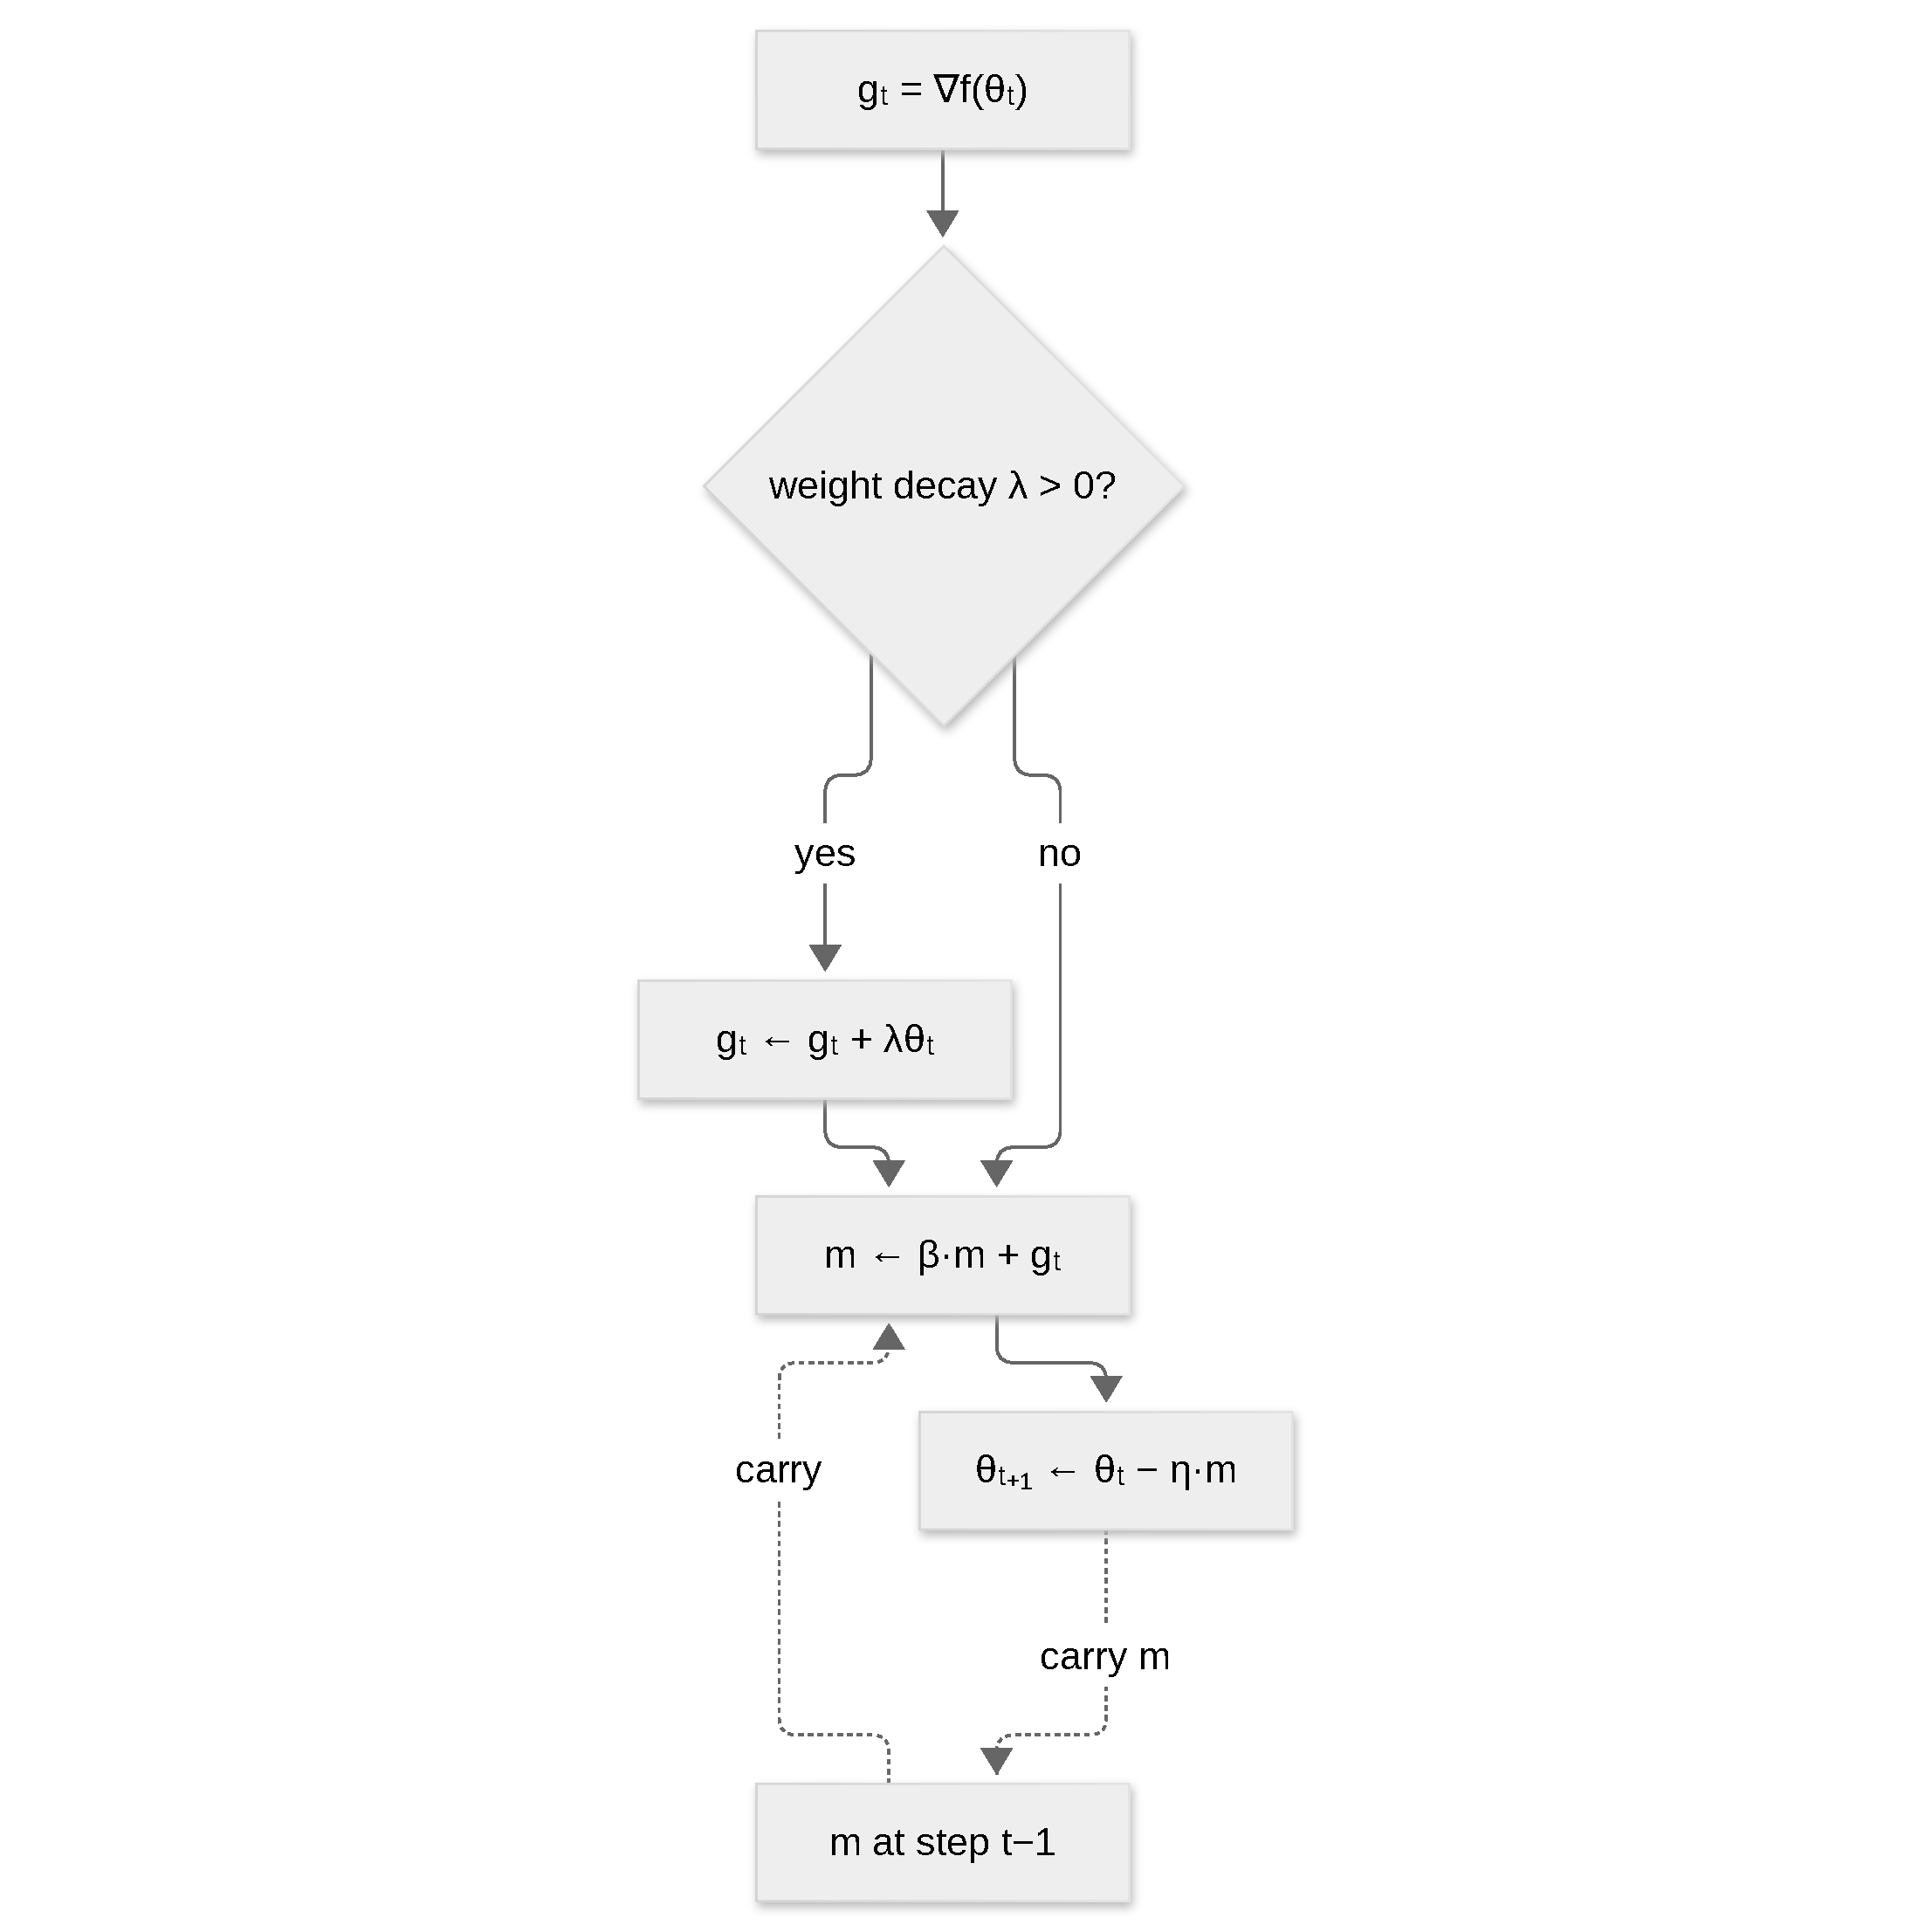
\includegraphics{figures/optimizers/sgd-momentum.pdf}}
\caption{Step flow of SGD with momentum: optional L2 weight decay, exponential momentum accumulation, and the fixed-step parameter update.}
\label{fig:opt-sgd-momentum}
\end{figure}
The classical update accumulates a momentum buffer and then applies a fixed learning rate. At each iteration $t$, the algorithm maintains an exponential moving average $m_t$ of past gradients:
\begin{align}
m_t &= \beta m_{t-1} + g_t \\
\theta_{t+1} &= \theta_t - \eta m_t
\end{align}
where $g_t = \nabla f(\theta_t)$, $\beta \in [0.8, 0.99]$ controls the momentum decay, and $\eta$ is the fixed learning rate. The momentum term acts as velocity: it accelerates movement in consistent directions while dampening oscillations in variable directions.

\begin{algorithm}[H]
\caption{SGD with Momentum}
\label{alg:sgd-momentum}
\begin{algorithmic}[1]
\Require Initial parameters $\theta_0$, learning rate $\eta$, momentum coefficient $\beta$, weight decay $\lambda$
\Ensure Updated parameters $\theta_T$
\State Initialize: momentum buffer $m \gets 0$
\For{$t = 0, 1, 2, \ldots, T-1$}
    \State Compute gradient: $g_t \gets \nabla f(\theta_t)$
    \If{weight\_decay $> 0$}
        \State $g_t \gets g_t + \lambda \theta_t$ \Comment{L2 regularization}
    \EndIf
    \State Update momentum: $m \gets \beta \cdot m + g_t$
    \State Update parameters: $\theta_{t+1} \gets \theta_t - \eta \cdot m$
\EndFor
\Return $\theta_T$
\end{algorithmic}
\end{algorithm}

\paragraph{Cons.}
\begin{itemize}[leftmargin=*]
\item Poor robustness to heterogeneous curvature: a single global rate cannot suit every parameter group.
\item Strong dependence on carefully engineered learning-rate schedules.
\end{itemize}

\paragraph{Pros.}
\begin{itemize}[leftmargin=*]
\item Low memory overhead: a single momentum buffer per parameter.
\item Strong generalization when tuned carefully, and a simple update to implement.
\end{itemize}

\paragraph{Adam and AdamW.}
\begin{figure}[H]
\centering
\fitfigure{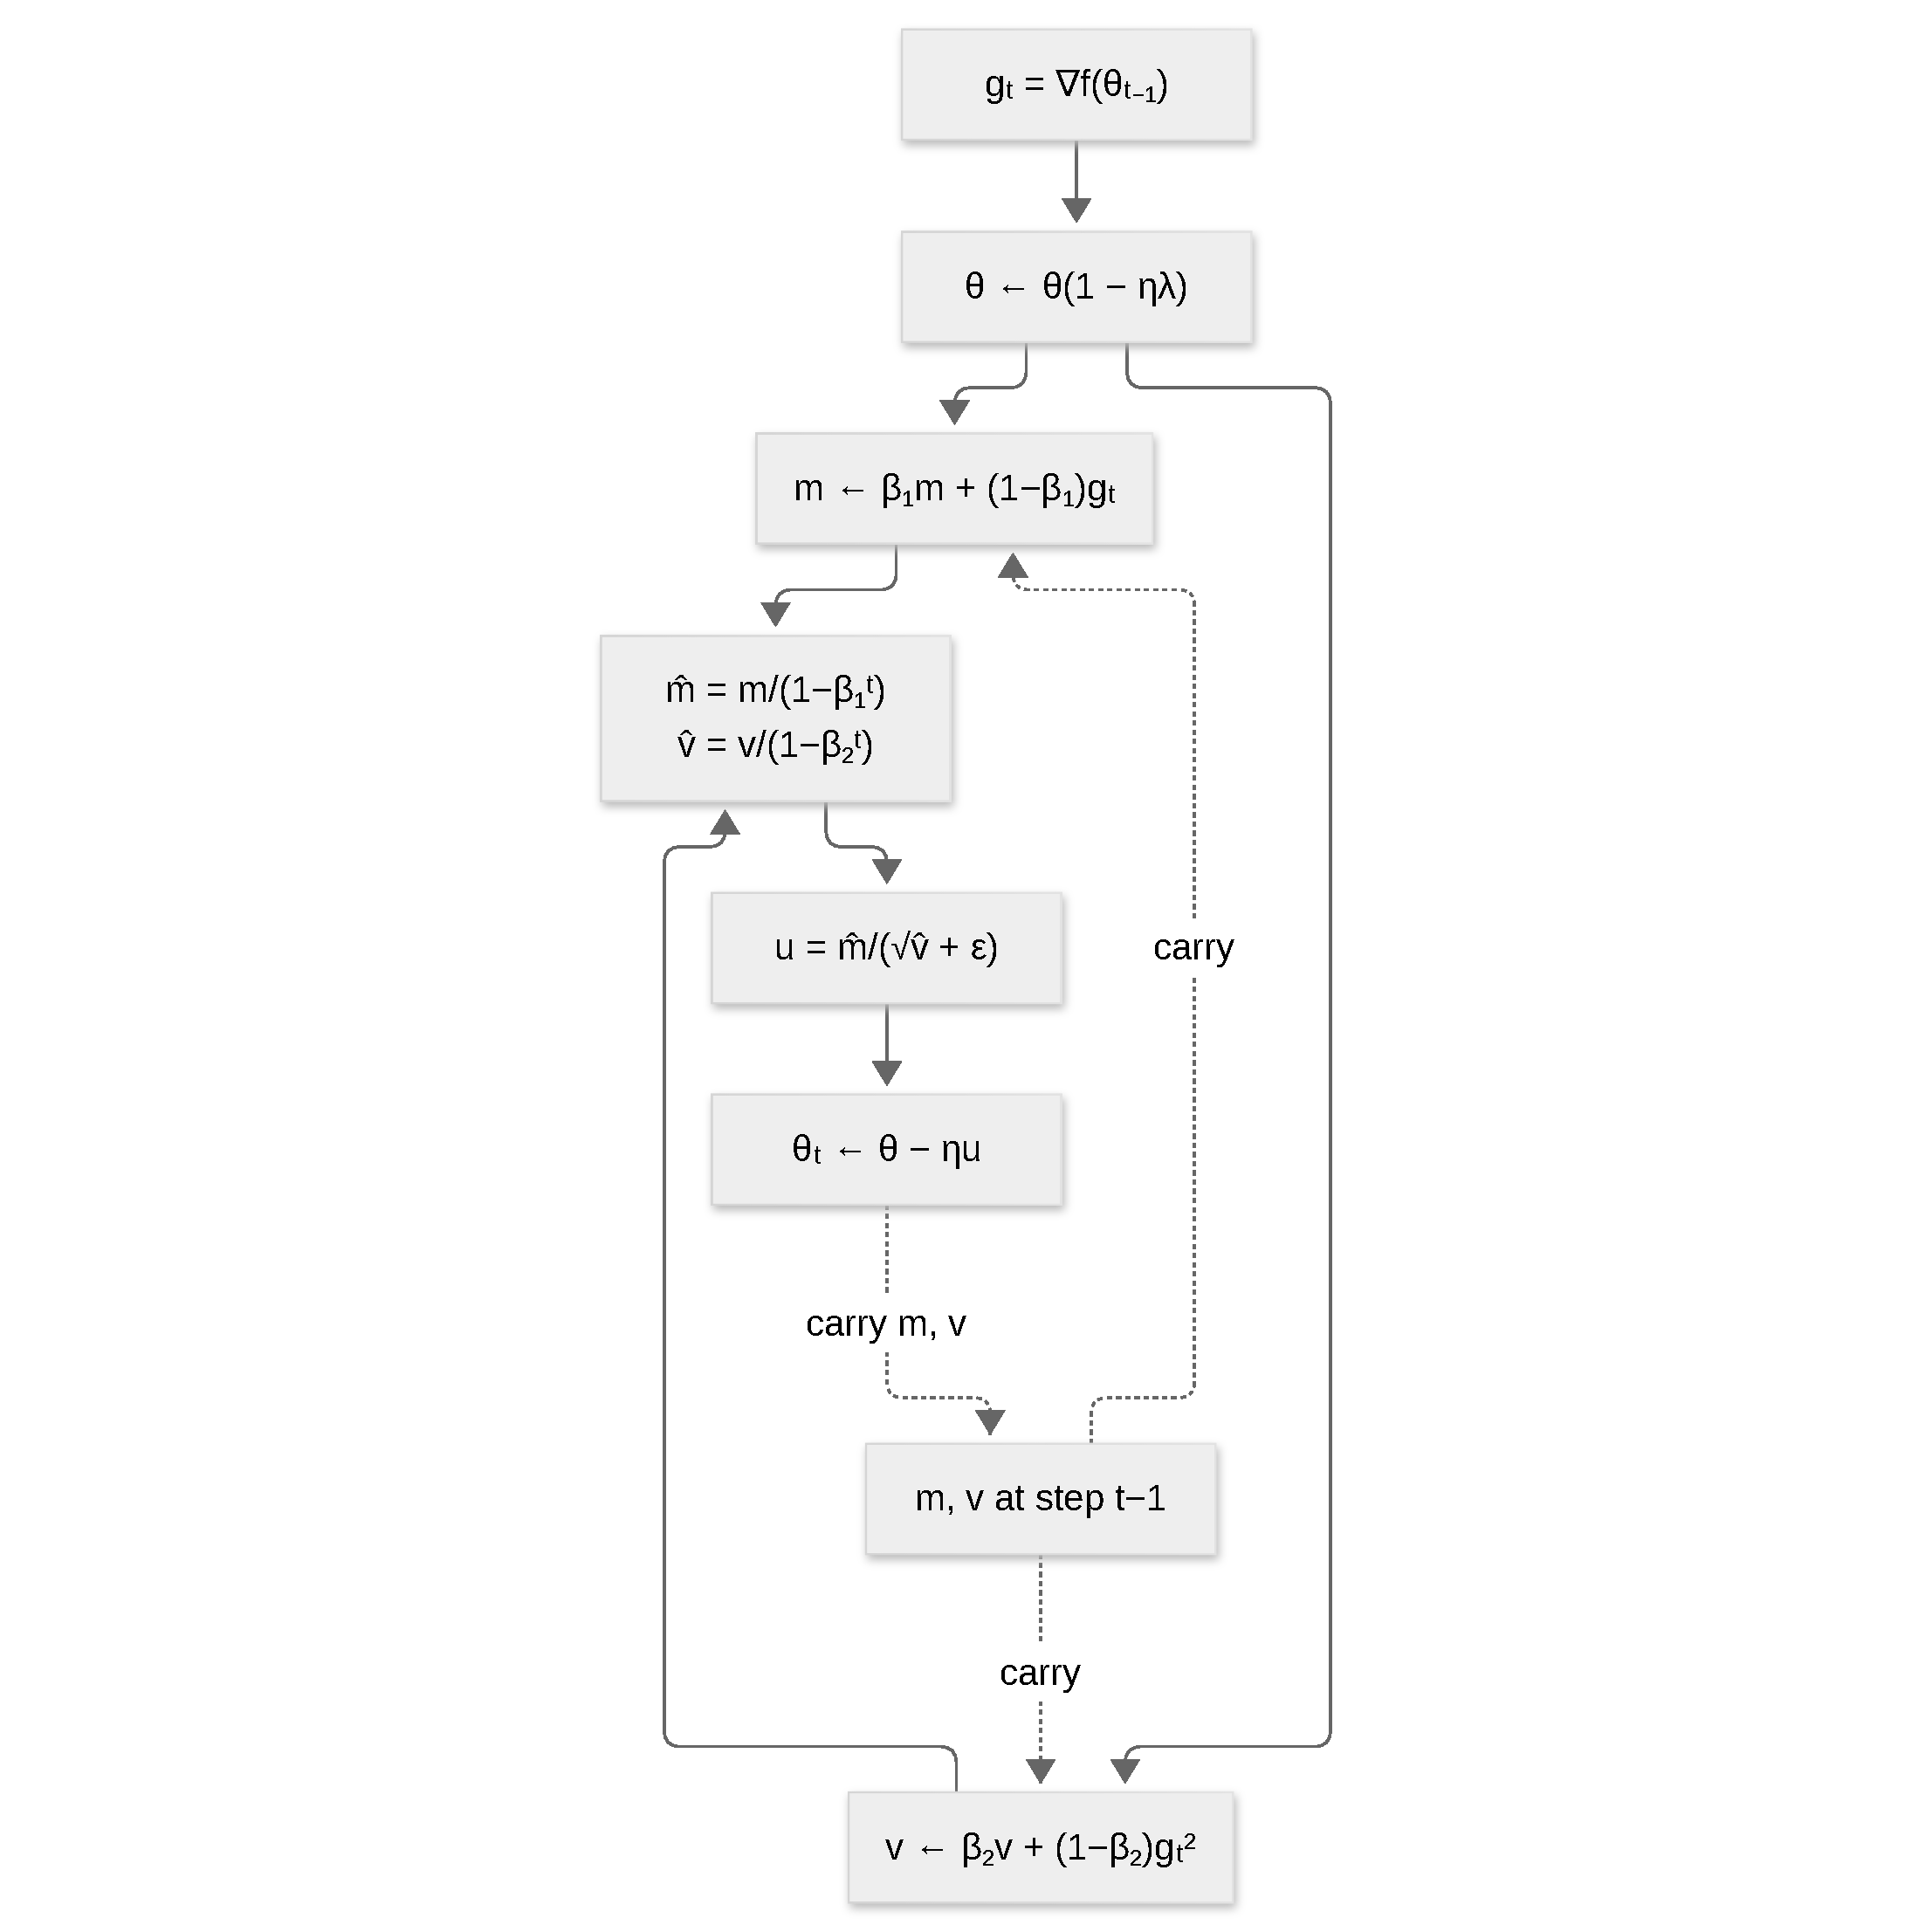
\includegraphics{figures/optimizers/adamw.pdf}}
\caption{Step flow of AdamW: decoupled weight decay, first- and second-moment EMAs, bias correction, and the element-wise adaptive update.}
\label{fig:opt-adamw}
\end{figure}
Adam tracks exponential moving averages of both first moment (mean) and second moment (uncentered variance) to achieve element-wise adaptive learning rates. The update rule is:
\begin{align}
m_t &= \beta_1 m_{t-1} + (1-\beta_1) g_t \\
v_t &= \beta_2 v_{t-1} + (1-\beta_2) g_t^2 \\
\hat{m}_t &= \frac{m_t}{1-\beta_1^t}, \quad \hat{v}_t = \frac{v_t}{1-\beta_2^t} \quad \text{(bias correction)} \\
\theta_{t+1} &= \theta_t - \eta \left(\frac{\hat{m}_t}{\sqrt{\hat{v}_t}+\epsilon}\right)
\end{align}
AdamW introduces a crucial modification: weight decay is applied directly to parameters (decoupled from gradients): $\theta_t \gets \theta_t(1-\eta\lambda)$ rather than adding $\lambda\theta_t$ to the gradient. This decoupling prevents the adaptive scaling from interfering with regularization strength.

\begin{algorithm}[H]
\caption{AdamW (Adam with Decoupled Weight Decay)}
\label{alg:adamw}
\begin{algorithmic}[1]
\Require Initial parameters $\theta_0$, learning rate $\eta$, exponential decay rates $\beta_1, \beta_2 \in [0,1)$
\Require Momentum constant $\epsilon$, weight decay $\lambda$
\Ensure Updated parameters $\theta_T$
\State Initialize: first moment $m \gets 0$, second moment $v \gets 0$, step counter $t \gets 0$
\For{$t = 1, 2, \ldots, T$}
    \State Compute gradient: $g_t \gets \nabla f(\theta_{t-1})$
    \State Weight decay (decoupled): $\theta_{t-1} \gets \theta_{t-1}(1 - \eta\lambda)$
    \State Update moments: $m \gets \beta_1 m + (1-\beta_1) g_t$
    \State $v \gets \beta_2 v + (1-\beta_2) g_t^2$
    \State Bias correction: $\hat{m} \gets m / (1 - \beta_1^t)$, $\hat{v} \gets v / (1 - \beta_2^t)$
    \State Update parameters: $\theta_t \gets \theta_{t-1} - \eta (\hat{m} / (\sqrt{\hat{v}} + \epsilon))$
\EndFor
\Return $\theta_T$
\end{algorithmic}
\end{algorithm}

\paragraph{Cons.}
\begin{itemize}[leftmargin=*]
\item Stores first and second moment tensors for every parameter, doubling optimizer-state memory relative to SGD.
\item Element-wise adaptive scaling can interfere with regularization unless weight decay is decoupled.
\end{itemize}

\paragraph{Pros.}
\begin{itemize}[leftmargin=*]
\item Practical baseline for transformer fine-tuning: fast convergence and forgiving to hyperparameter variation.
\item Decoupled weight decay keeps the regularization strength independent of the adaptive scaling.
\end{itemize}

\paragraph{RAdam (Rectified Adam).}
\begin{figure}[H]
\centering
\fitfigure{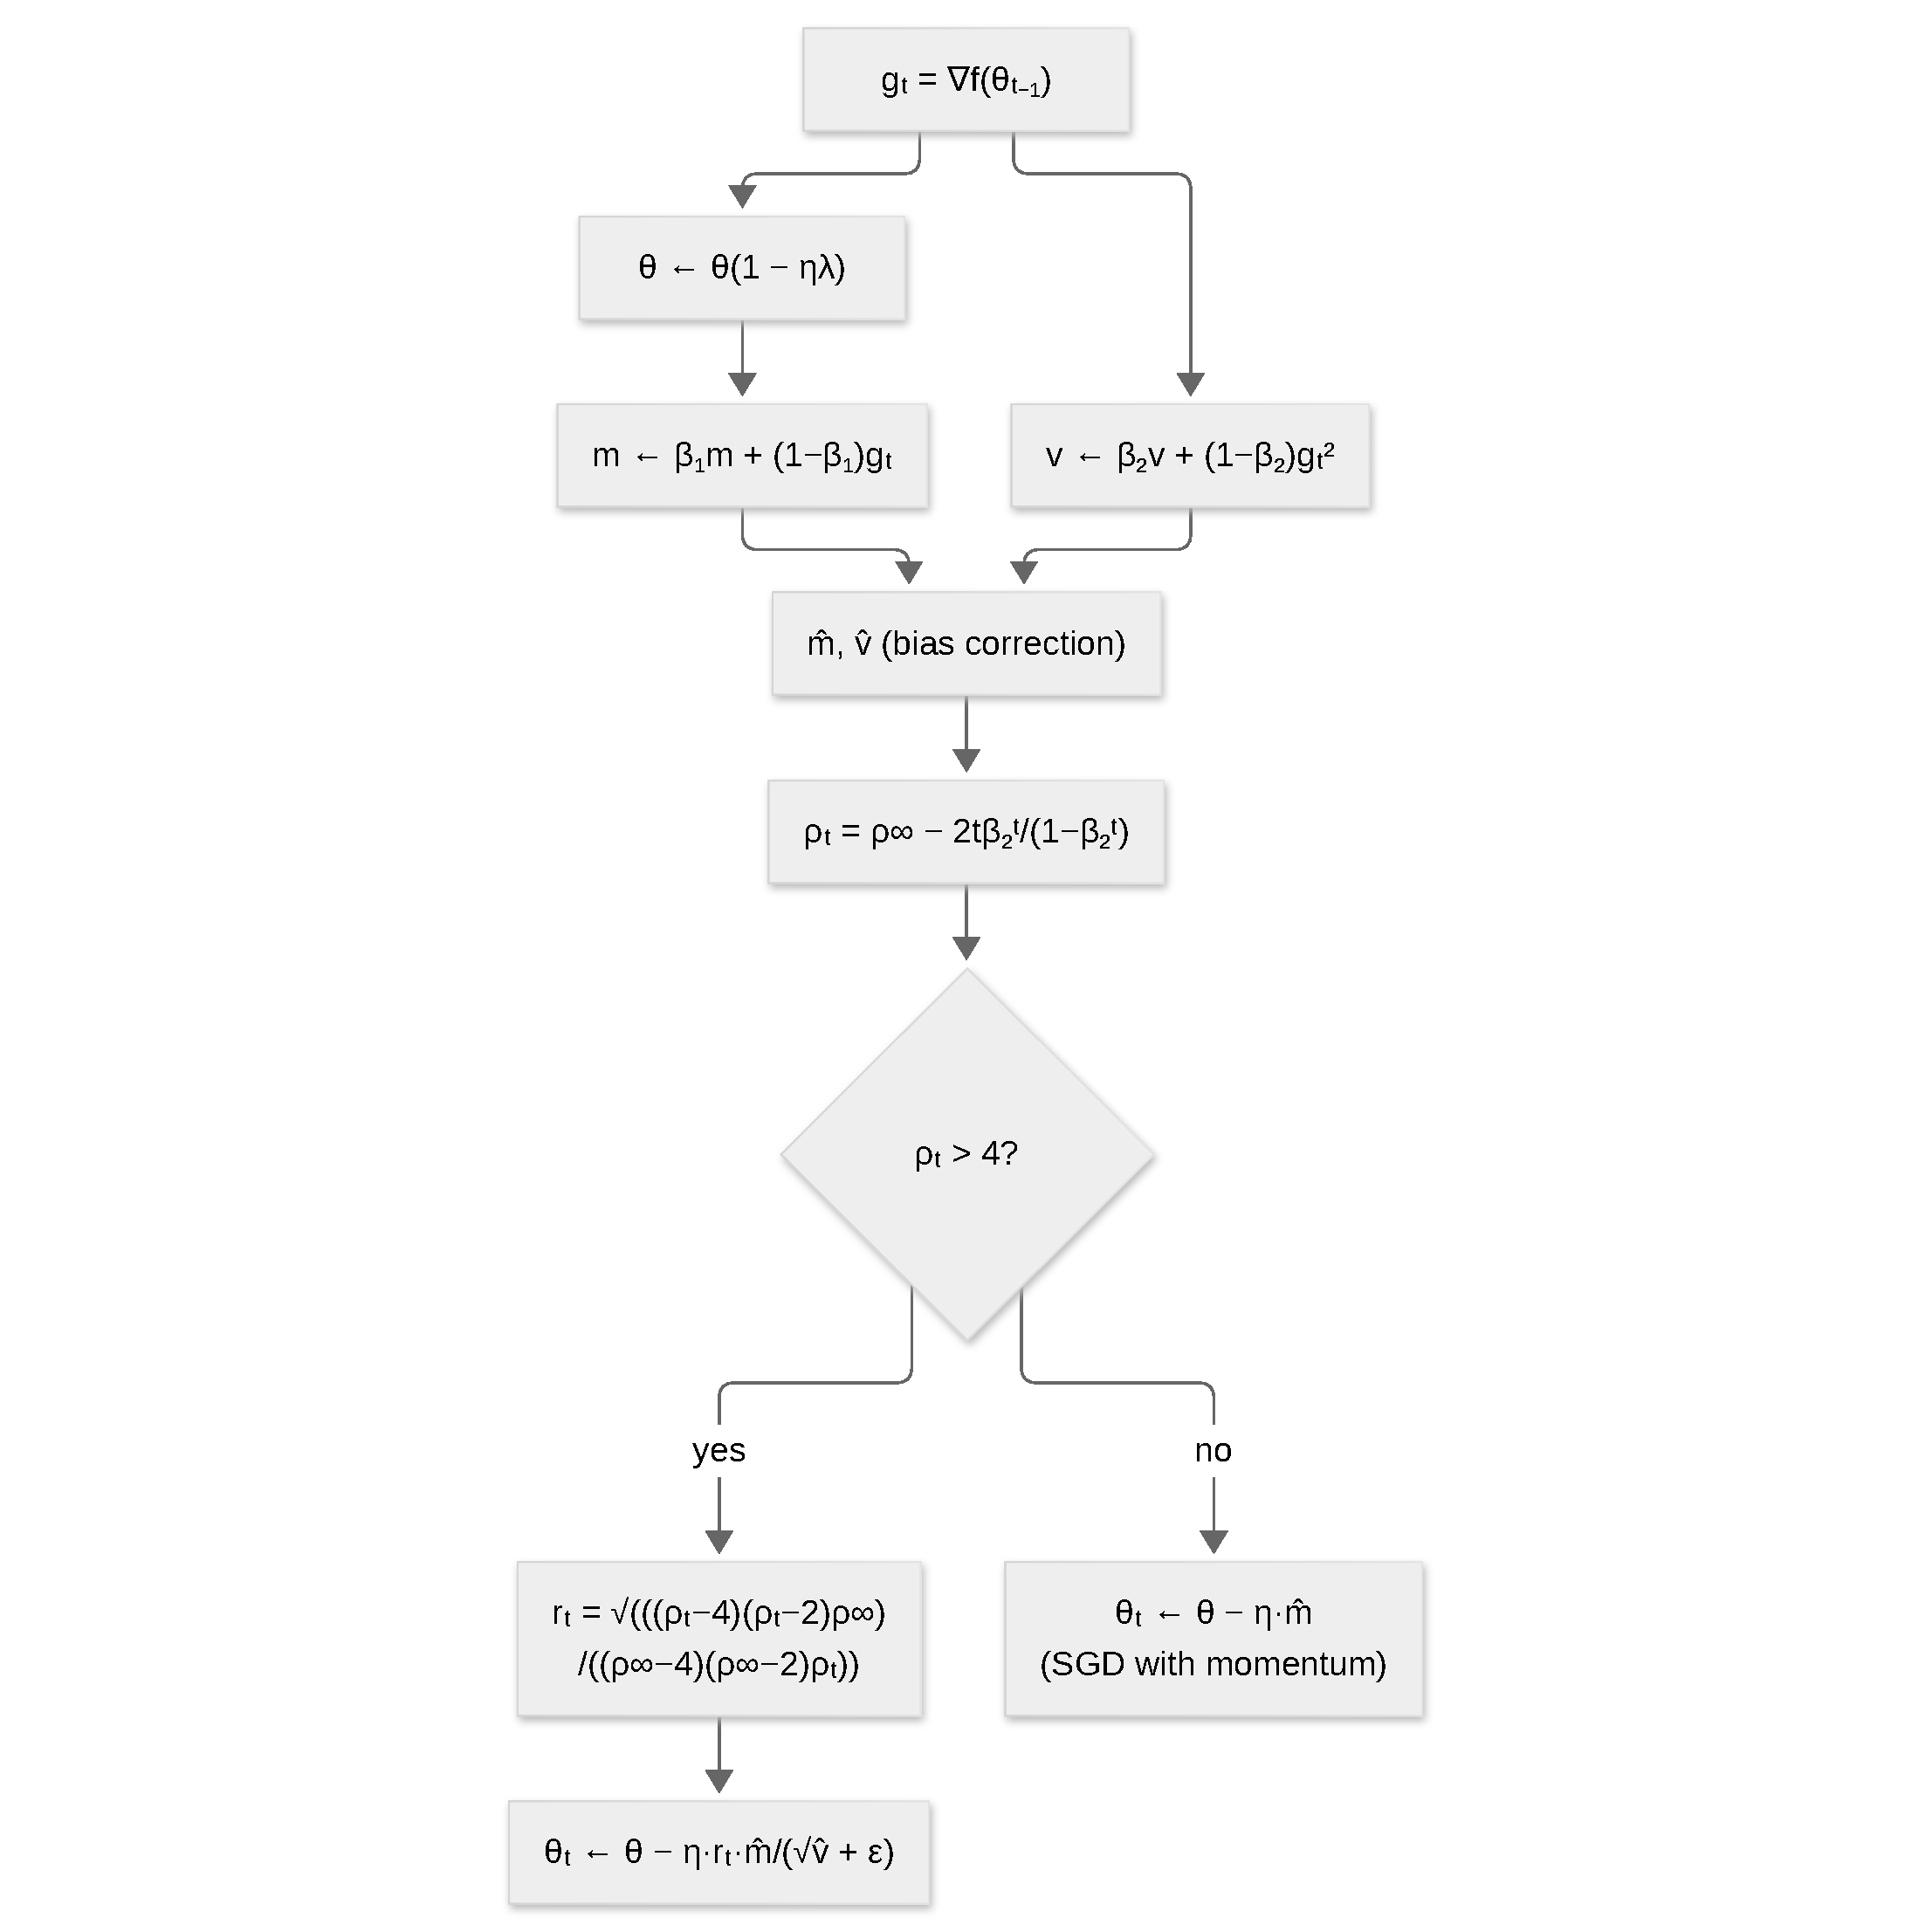
\includegraphics{figures/optimizers/radam.pdf}}
\caption{Step flow of RAdam: SMA-window rectification with an early-step fallback to momentum SGD.}
\label{fig:opt-radam}
\end{figure}
RAdam addresses Adam's instability in early training by dynamically rectifying the adaptive learning rate. The key observation is that the second moment $v_t$ has very high variance in the first few steps, causing unreliable adaptive scaling. RAdam computes the effective simple moving average (SMA) window length:
\[\rho_t = \rho_{\infty} - \frac{2t\beta_2^t}{1-\beta_2^t}, \quad \text{where} \quad \rho_{\infty} = \frac{2}{1-\beta_2}-1\]
When $\rho_t > 4$ (sufficient samples for variance estimation), RAdam applies adaptive scaling with a rectification term:
\[r_t = \sqrt{\frac{(\rho_t-4)(\rho_t-2)\rho_{\infty}}{(\rho_{\infty}-4)(\rho_{\infty}-2)\rho_t}}, \quad \theta_{t+1} = \theta_t - \eta r_t \frac{\hat{m}_t}{\sqrt{\hat{v}_t}+\epsilon}\]
When $\rho_t \leq 4$, RAdam falls back to SGD with momentum: $\theta_{t+1} = \theta_t - \eta\hat{m}_t$.

\begin{algorithm}[H]
\caption{RAdam (Rectified Adam)}
\label{alg:radam}
\begin{algorithmic}[1]
\Require Initial parameters $\theta_0$, learning rate $\eta$, $\beta_1, \beta_2$, weight decay $\lambda$
\Ensure Updated parameters $\theta_T$
\State Initialize: $m \gets 0$, $v \gets 0$, $t \gets 0$
\State Compute: $\rho_\infty \gets 2/(1-\beta_2) - 1$
\For{$t = 1, 2, \ldots, T$}
    \State $g_t \gets \nabla f(\theta_{t-1})$
    \If{weight\_decay $> 0$}
        \State $\theta_{t-1} \gets \theta_{t-1}(1 - \eta\lambda)$
    \EndIf
    \State $m \gets \beta_1 m + (1-\beta_1) g_t$
    \State $v \gets \beta_2 v + (1-\beta_2) g_t^2$
    \State $\hat{m} \gets m/(1-\beta_1^t)$, $\hat{v} \gets v/(1-\beta_2^t)$
    \State $\rho_t \gets \rho_\infty - 2t \beta_2^t / (1 - \beta_2^t)$
    \If{$\rho_t > 4$}
        \State $r_t \gets \sqrt{((\rho_t-4)(\rho_t-2)\rho_\infty) / ((\rho_\infty-4)(\rho_\infty-2)\rho_t)}$
        \State $\theta_t \gets \theta_{t-1} - \eta r_t \hat{m} / (\sqrt{\hat{v}} + \epsilon)$
    \Else
        \State $\theta_t \gets \theta_{t-1} - \eta \hat{m}$ \Comment{SGD with momentum}
    \EndIf
\EndFor
\Return $\theta_T$
\end{algorithmic}
\end{algorithm}

\paragraph{Cons.}
\begin{itemize}[leftmargin=*]
\item Adds rectification bookkeeping on top of Adam's moment state.
\item The benefit shrinks when a well-tuned warmup schedule is already in use.
\end{itemize}

\paragraph{Pros.}
\begin{itemize}[leftmargin=*]
\item Eliminates the need for manual learning-rate warmup by rectifying the adaptive rate.
\item Falls back gracefully to momentum SGD while variance estimates are unreliable, improving robustness.
\end{itemize}

\subsection{Advanced Momentum and Variance Reduction (2024--2025)}
\paragraph{Adan (Adaptive Nesterov Momentum).}
\begin{figure}[H]
\centering
\fitfigure{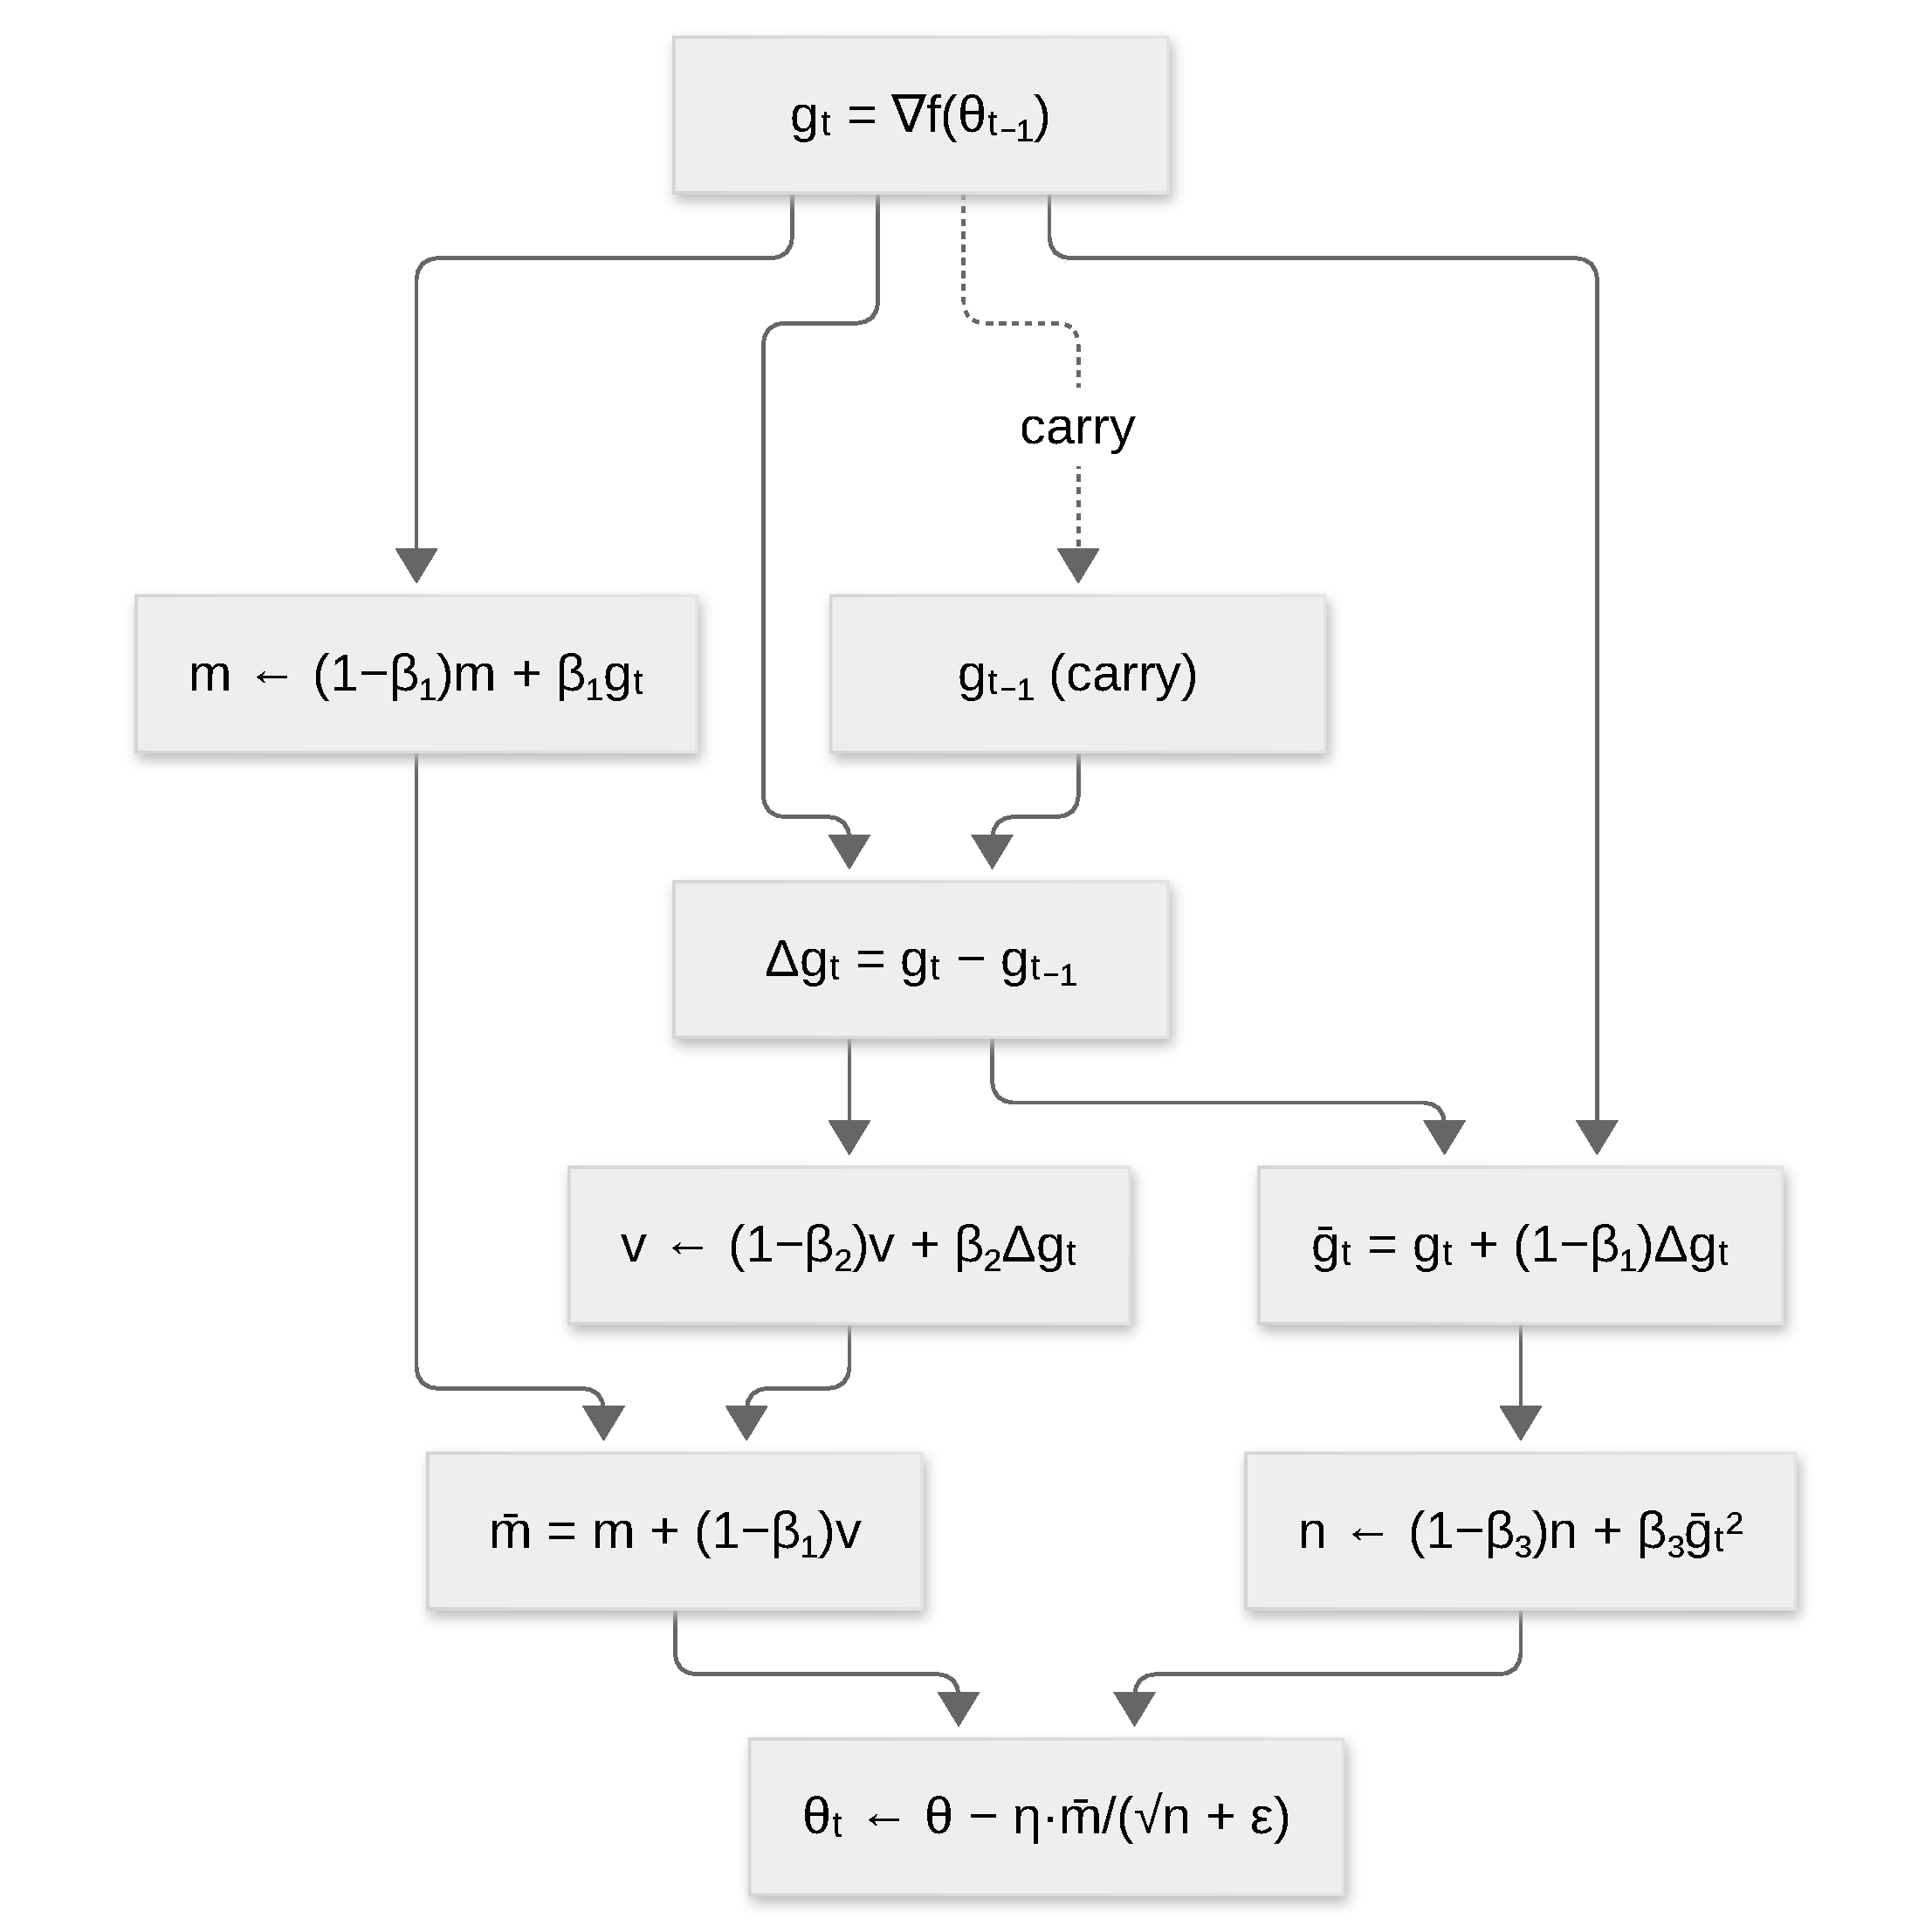
\includegraphics{figures/optimizers/adan.pdf}}
\caption{Step flow of Adan: Nesterov momentum estimation from the gradient difference, with three state buffers and a combined momentum step.}
\label{fig:opt-adan}
\end{figure}
Adan reformulates Nesterov acceleration without the extra gradient computation required by classical Nesterov SGD. The algorithm maintains three momentum buffers:
\begin{align}
m_t &= (1-\beta_1)m_{t-1} + \beta_1 g_t \quad\text{(first moment)} \\
v_t &= (1-\beta_2)v_{t-1} + \beta_2(g_t - g_{t-1}) \quad\text{(velocity/gradient difference)} \\
n_t &= (1-\beta_3)n_{t-1} + \beta_3[g_t + (1-\beta_1)(g_t-g_{t-1})]^2 \quad\text{(Nesterov second moment)}
\end{align}
The \textbf{Nesterov Momentum Estimation} (NME) term $\bar{g}_t = g_t + (1-\beta_1)(g_t-g_{t-1})$ estimates the gradient at a future position without evaluating it. The update combines momentum with velocity:
\[\bar{m}_t = m_t + (1-\beta_1)v_t, \quad \theta_{t+1} = \theta_t - \eta\frac{\bar{m}_t}{\sqrt{n_t}+\epsilon}\]

\begin{algorithm}[H]
\caption{Adan (Adaptive Nesterov Momentum)}
\label{alg:adan}
\begin{algorithmic}[1]
\Require Initial parameters $\theta_0$, learning rate $\eta$, $\beta_1, \beta_2, \beta_3 \in (0,1)$
\Ensure Updated parameters $\theta_T$
\State Initialize: $m \gets 0$, $v \gets 0$, $n \gets 0$, $g_{-1} \gets 0$ (previous gradient)
\For{$t = 1, 2, \ldots, T$}
    \State $g_t \gets \nabla f(\theta_{t-1})$
    \State $m \gets (1-\beta_1) m + \beta_1 g_t$
    \State $\Delta g_t \gets g_t - g_{t-1}$
    \State $v \gets (1-\beta_2) v + \beta_2 \Delta g_t$
    \State Nesterov estimation: $\bar{g}_t \gets g_t + (1-\beta_1) \Delta g_t$
    \State $n \gets (1-\beta_3) n + \beta_3 \bar{g}_t^2$
    \State Combined momentum: $\bar{m} \gets m + (1-\beta_1) v$
    \State $\theta_t \gets \theta_{t-1} - \eta (\bar{m} / (\sqrt{n} + \epsilon))$
    \State $g_{t-1} \gets g_t$
\EndFor
\Return $\theta_T$
\end{algorithmic}
\end{algorithm}

\paragraph{Cons.}
\begin{itemize}[leftmargin=*]
\item Three momentum-like buffers increase memory overhead relative to Adam.
\item Additional gradient-difference bookkeeping per step.
\end{itemize}

\paragraph{Pros.}
\begin{itemize}[leftmargin=*]
\item Nesterov-style acceleration without an extra gradient evaluation.
\item Fast convergence across diverse architectures (CNNs, GANs, transformers).
\end{itemize}

\paragraph{ADOPT (Adam with Optimal Pruned Tuning).}
\begin{figure}[H]
\centering
\fitfigure{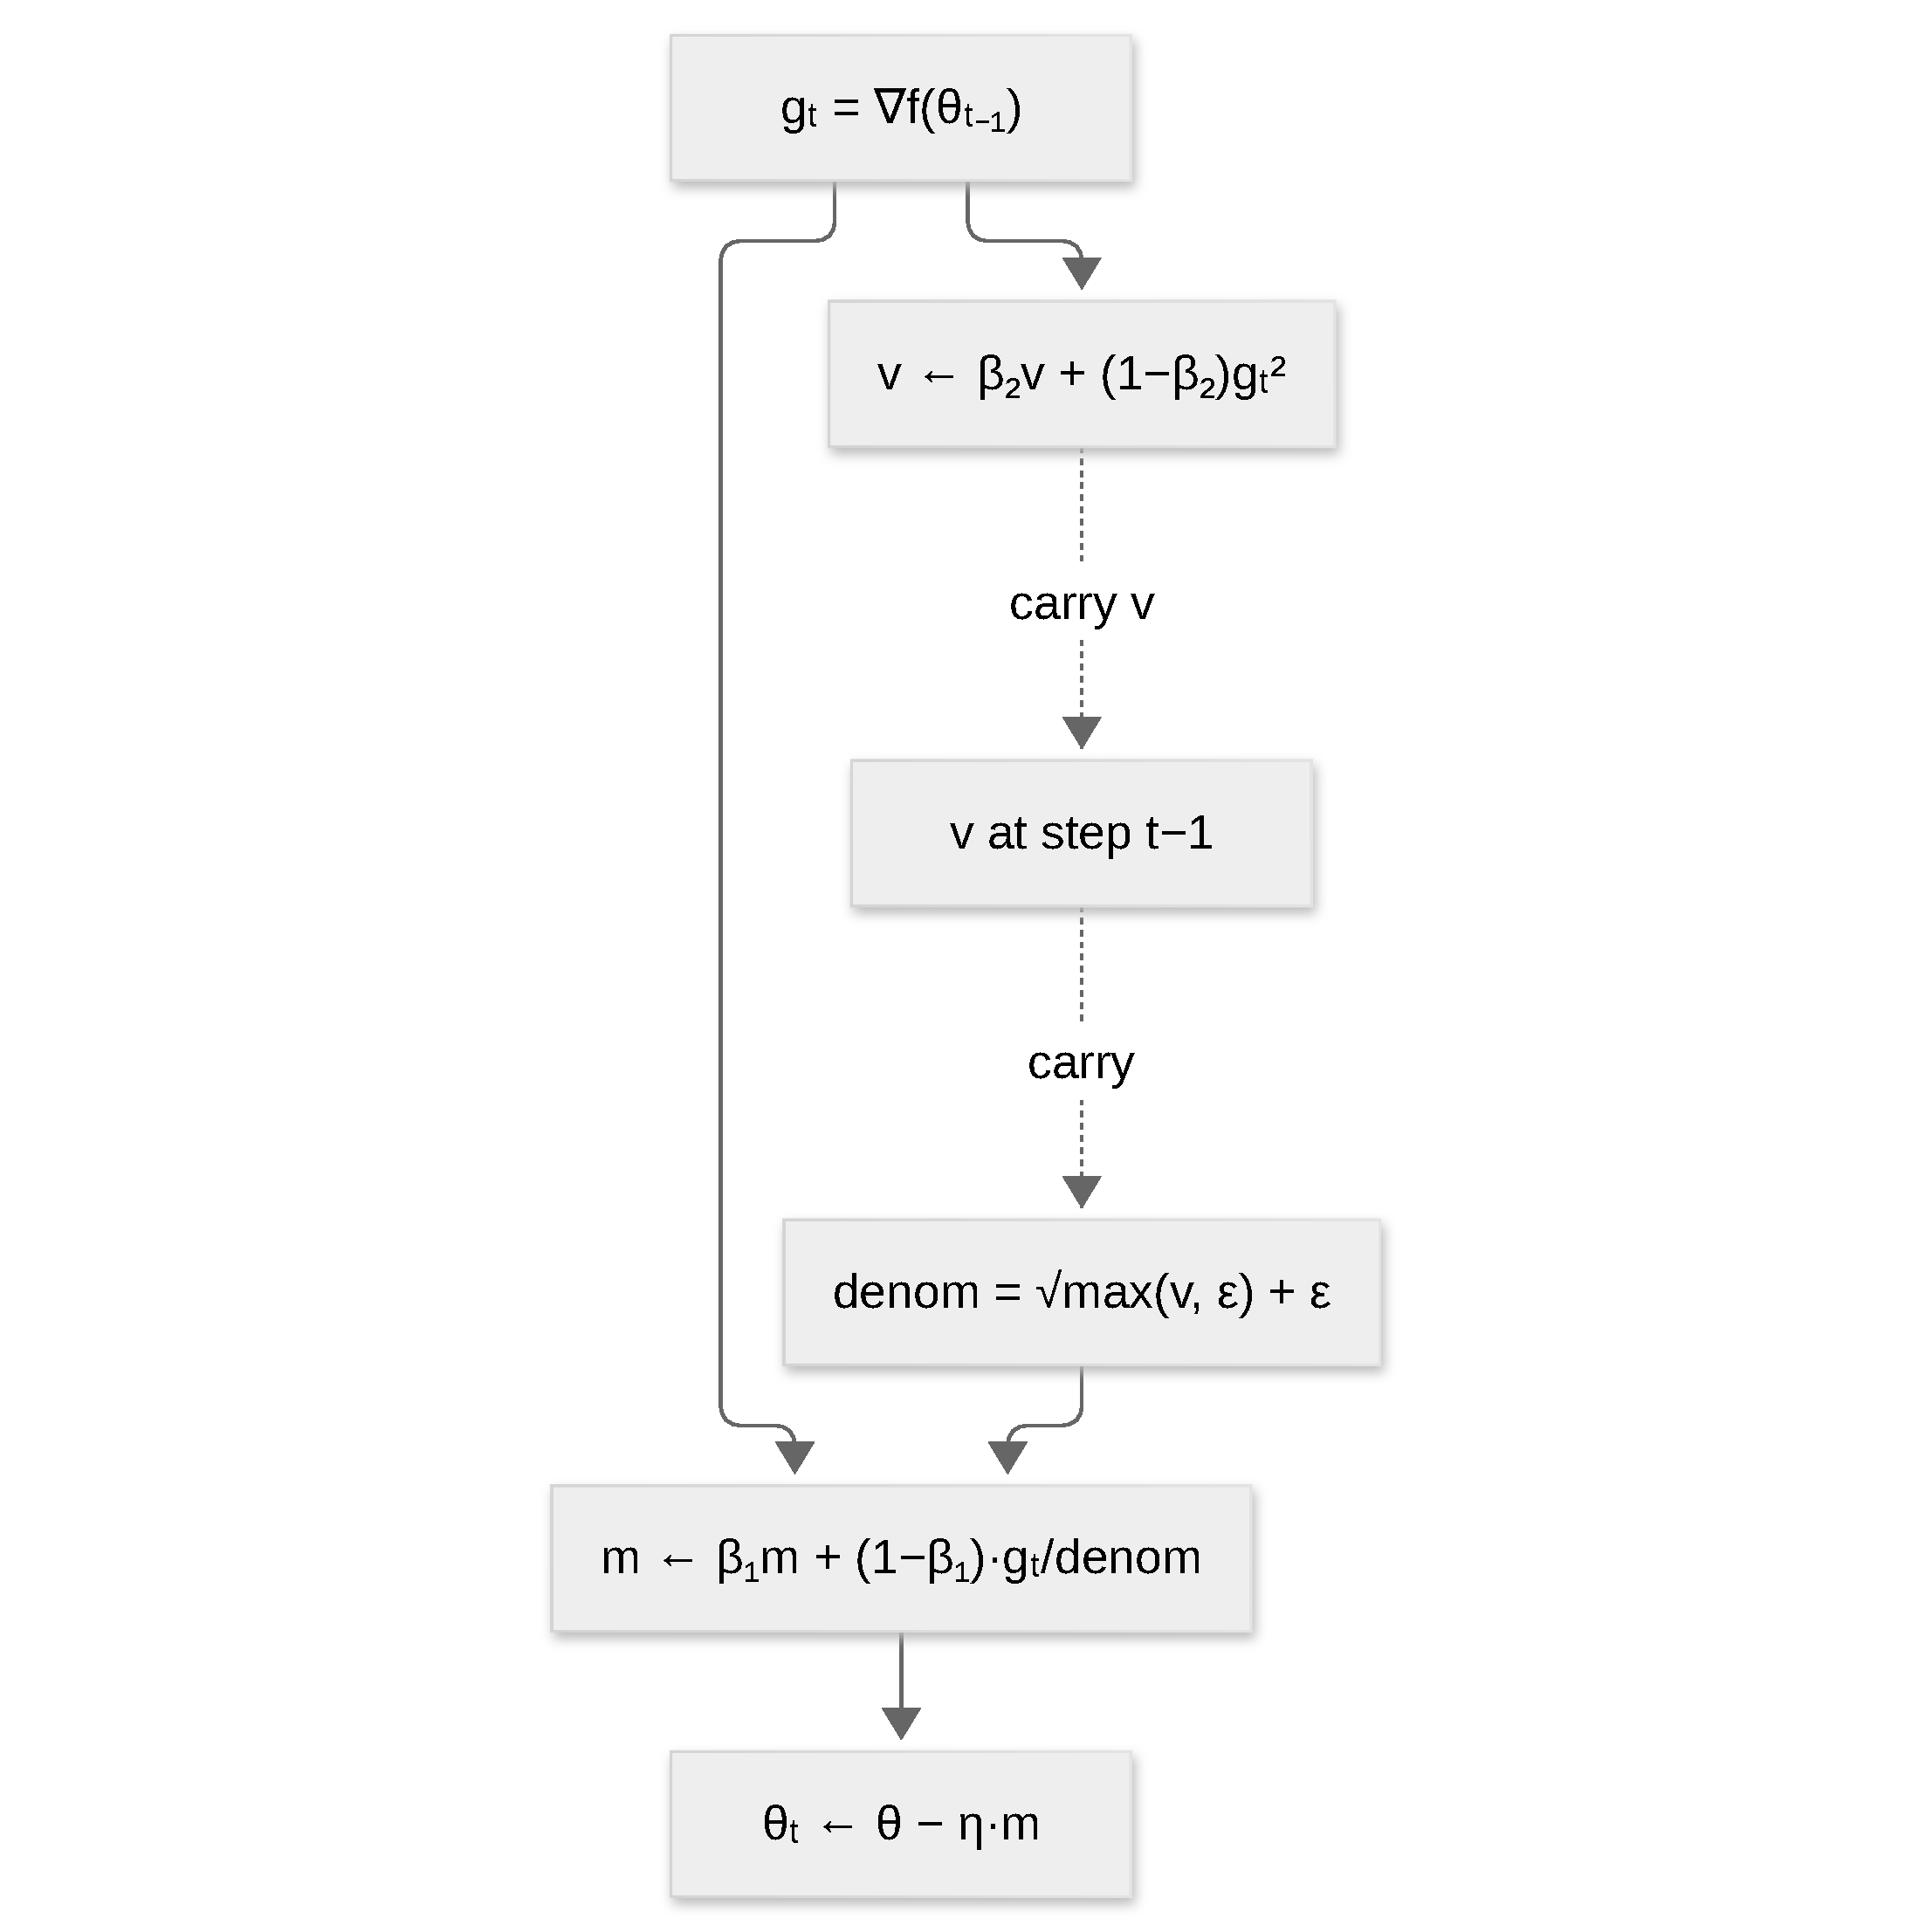
\includegraphics{figures/optimizers/adopt.pdf}}
\caption{Step flow of ADOPT: the second moment from the previous step normalizes the current gradient before the first-moment update.}
\label{fig:opt-adopt}
\end{figure}
ADOPT fixes a fundamental theoretical issue in Adam: the gradient appears in both the first moment and second moment estimates, creating circularity. ADOPT \textbf{decouples} by using the previous step's second moment for the denominator:
\begin{align}
v_t &= \beta_2 v_{t-1} + (1-\beta_2)g_t^2 \\
m_t &= \beta_1 m_{t-1} + (1-\beta_1)\frac{g_t}{\sqrt{v_{t-1}}+\epsilon} \quad\text{(uses $v_{t-1}$, not $v_t$)} \\
\theta_{t+1} &= \theta_t - \eta m_t
\end{align}

\begin{algorithm}[H]
\caption{ADOPT (Adam with Optimal Pruned Tuning)}
\label{alg:adopt}
\begin{algorithmic}[1]
\Require Initial parameters $\theta_0$, learning rate $\eta$, $\beta_1, \beta_2$, tolerance $\epsilon$
\Ensure Updated parameters $\theta_T$
\State Initialize: $m \gets 0$, $v \gets 0$
\For{$t = 1, 2, \ldots, T$}
    \State $g_t \gets \nabla f(\theta_{t-1})$
    \If{weight\_decay $> 0$}
        \State $\theta_{t-1} \gets \theta_{t-1}(1 - \eta\lambda)$
    \EndIf
    \State Use \textbf{previous} second moment: $\text{denom} \gets \sqrt{\max(v, \epsilon)} + \epsilon$
    \State Update first moment using previous variance: $m \gets \beta_1 m + (1-\beta_1)(g_t / \text{denom})$
    \State Update second moment with \textbf{current} gradient: $v \gets \beta_2 v + (1-\beta_2) g_t^2$
    \State $\theta_t \gets \theta_{t-1} - \eta m$
\EndFor
\Return $\theta_T$
\end{algorithmic}
\end{algorithm}

\paragraph{Cons.}
\begin{itemize}[leftmargin=*]
\item Requires keeping the previous second moment as an explicit denominator.
\item Empirical gains are architecture- and tuning-dependent.
\end{itemize}

\paragraph{Pros.}
\begin{itemize}[leftmargin=*]
\item Removes Adam's gradient circularity and attains the optimal convergence rate $O(1/\sqrt{T})$ with \textbf{any} $\beta_2 \in (0,1)$, without bounded-noise assumptions.
\item Drop-in Adam replacement with comparable or superior empirical performance across vision, NLP, RL, and generative modeling.
\end{itemize}

\paragraph{AdEMAMix (Exponential Moving Average Mixture).}
\begin{figure}[H]
\centering
\fitfigure{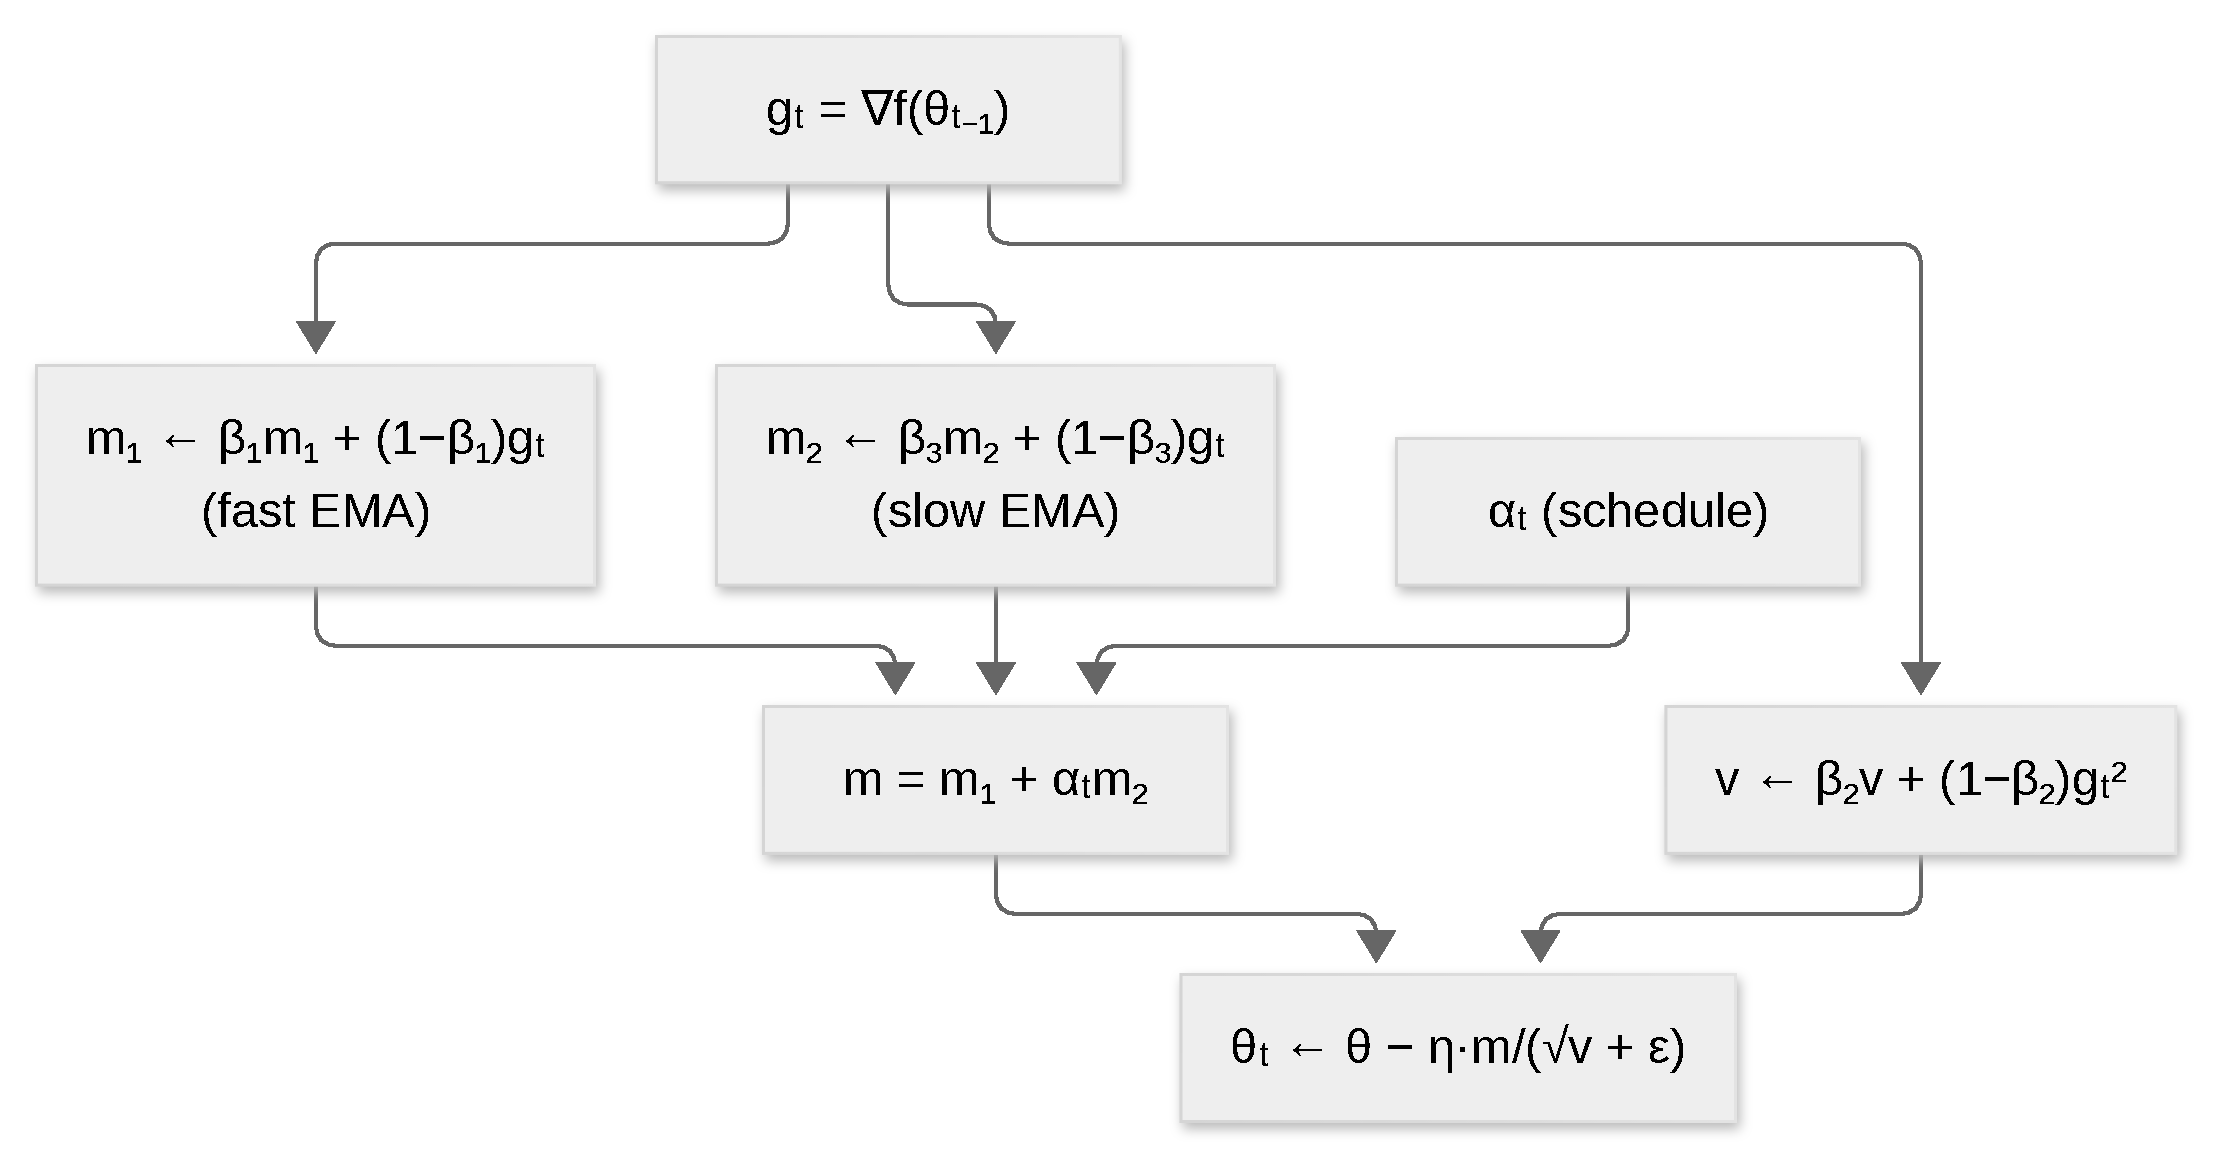
\includegraphics{figures/optimizers/ademamix.pdf}}
\caption{Step flow of AdEMAMix: parallel fast and slow gradient EMAs, mixed with a scheduled weight $\alpha_t$ before the adaptive update.}
\label{fig:opt-ademamix}
\end{figure}
AdEMAMix replaces Adam's single EMA of gradients with a \textbf{mixture of two EMAs}: one fast-decaying and one slow-decaying. This addresses the observation that gradients remain informative over tens of thousands of steps, not just hundreds:
\begin{align}
m_{1,t} &= \beta_1 m_{1,t-1} + (1-\beta_1)g_t \quad\text{(fast EMA, $\beta_1 \approx 0.9$)} \\
m_{2,t} &= \beta_3 m_{2,t-1} + (1-\beta_3)g_t \quad\text{(slow EMA, $\beta_3 \approx 0.9999$)} \\
v_t &= \beta_2 v_{t-1} + (1-\beta_2)g_t^2 \\
m_t &= m_{1,t} + \alpha_t m_{2,t} \quad\text{(mixture with scheduled weight $\alpha_t$)} \\
\theta_{t+1} &= \theta_t - \eta\frac{m_t}{\sqrt{v_t}+\epsilon}
\end{align}
The mixture weight $\alpha_t$ typically increases during training, allowing the fast EMA to provide immediate adaptation while the slow EMA accumulates long-range gradient correlations.

\begin{algorithm}[H]
\caption{AdEMAMix (Exponential Moving Average Mixture)}
\label{alg:ademamix}
\begin{algorithmic}[1]
\Require Initial parameters $\theta_0$, learning rate $\eta$, $\beta_1$ (fast), $\beta_3$ (slow), $\beta_2$ (second moment)
\Require Mixture weight $\alpha_t$ (typically increasing), tolerance $\epsilon$
\Ensure Updated parameters $\theta_T$
\State Initialize: $m_1 \gets 0$ (fast EMA), $m_2 \gets 0$ (slow EMA), $v \gets 0$
\For{$t = 1, 2, \ldots, T$}
    \State $g_t \gets \nabla f(\theta_{t-1})$
    \If{weight\_decay $> 0$}
        \State $\theta_{t-1} \gets \theta_{t-1}(1 - \eta\lambda)$
    \EndIf
    \State $m_1 \gets \beta_1 m_1 + (1-\beta_1) g_t$ \Comment{Fast EMA}
    \State $m_2 \gets \beta_3 m_2 + (1-\beta_3) g_t$ \Comment{Slow EMA}
    \State $v \gets \beta_2 v + (1-\beta_2) g_t^2$
    \State $m_t \gets m_1 + \alpha_t m_2$ \Comment{Mixture}
    \State $\theta_t \gets \theta_{t-1} - \eta (m_t / (\sqrt{v} + \epsilon))$
\EndFor
\Return $\theta_T$
\end{algorithmic}
\end{algorithm}

\paragraph{Cons.}
\begin{itemize}[leftmargin=*]
\item Two gradient EMAs plus the second moment roughly triple Adam's optimizer state.
\item The mixture schedule $\alpha_t$ adds a hyperparameter to tune.
\end{itemize}

\paragraph{Pros.}
\begin{itemize}[leftmargin=*]
\item Exploits gradient information that remains informative over tens of thousands of steps.
\item A 1.3B model on 101B tokens matches AdamW on 197B tokens (95\% data-efficiency gain), suggesting reduced forgetting.
\end{itemize}

\paragraph{MARS (Make Adaptive learning Rates Shine).}
\begin{figure}[H]
\centering
\fitfigure{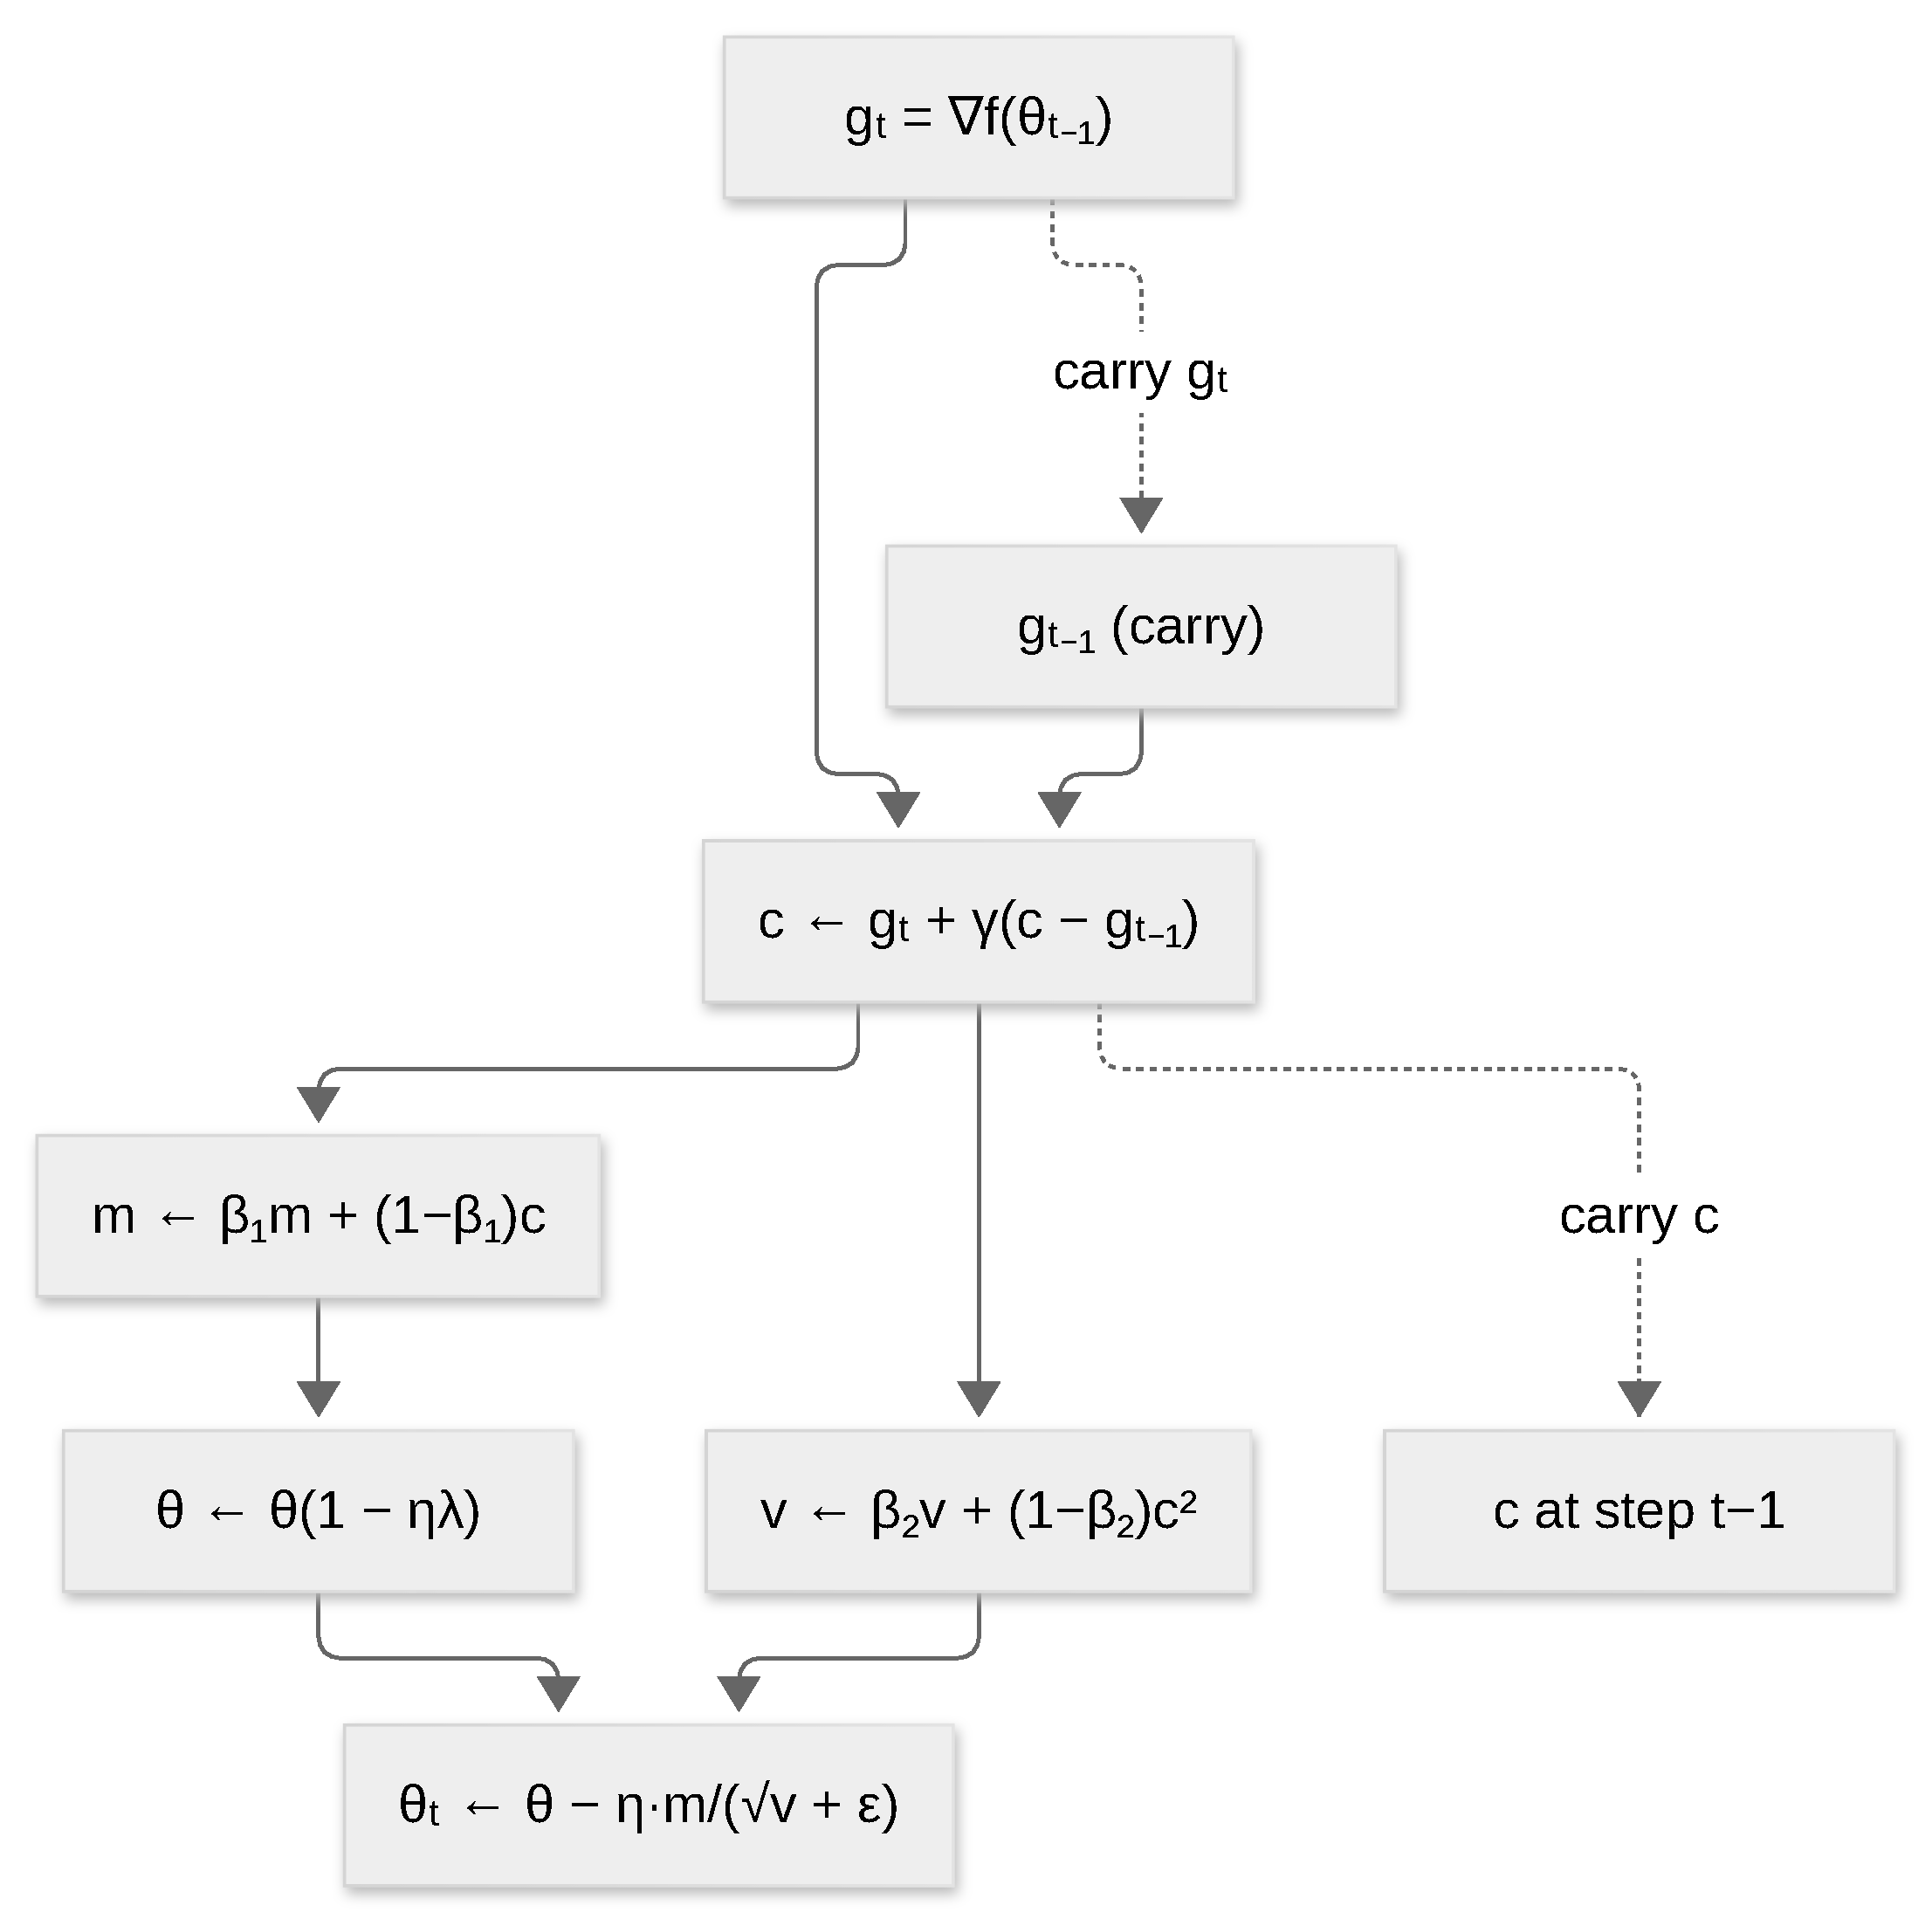
\includegraphics{figures/optimizers/mars.pdf}}
\caption{Step flow of MARS: a recursive variance-reduced gradient estimate feeding Adam-style first and second moments.}
\label{fig:opt-mars}
\end{figure}
MARS combines preconditioned gradient methods (e.g., AdamW) with \textbf{variance reduction} via scaled stochastic recursive momentum. The core innovation is a variance-reduced gradient estimate:
\begin{align}
c_t &= g_t + \gamma(c_{t-1} - g_{t-1}) \quad\text{(SVRG-style recursive estimate)} \\
m_t &= \beta_1 m_{t-1} + (1-\beta_1)c_t \\
v_t &= \beta_2 v_{t-1} + (1-\beta_2)c_t^2 \\
\theta_{t+1} &= \theta_t - \eta\frac{m_t}{\sqrt{v_t}+\epsilon}
\end{align}
where $\gamma \in [0.01, 0.1]$ controls how much historical gradient information is retained. The variance-reduced gradient $c_t$ acts as an implicit noise filter, amplifying consistent signal directions and dampening contradictory noise.

\begin{algorithm}[H]
\caption{MARS (Make Adaptive learning Rates Shine)}
\label{alg:mars}
\begin{algorithmic}[1]
\Require Initial parameters $\theta_0$, learning rate $\eta$, $\beta_1, \beta_2$, weight decay $\lambda$
\Require Variance reduction coefficient $\gamma \in [0.01, 0.1]$
\Ensure Updated parameters $\theta_T$
\State Initialize: $m \gets 0$, $v \gets 0$, $c \gets 0$ (variance-reduced gradient), $g_{-1} \gets 0$
\For{$t = 1, 2, \ldots, T$}
    \State $g_t \gets \nabla f(\theta_{t-1})$
    \State Variance reduction: $c \gets g_t + \gamma(c - g_{t-1})$
    \State $m \gets \beta_1 m + (1-\beta_1) c$
    \State $v \gets \beta_2 v + (1-\beta_2) c^2$
    \If{weight\_decay $> 0$}
        \State $\theta_{t-1} \gets \theta_{t-1}(1 - \eta\lambda)$
    \EndIf
    \State $\theta_t \gets \theta_{t-1} - \eta (m / (\sqrt{v} + \epsilon))$
    \State $g_{t-1} \gets g_t$
\EndFor
\Return $\theta_T$
\end{algorithmic}
\end{algorithm}

\paragraph{Cons.}
\begin{itemize}[leftmargin=*]
\item Stores the variance-reduced gradient and the previous gradient in addition to Adam's moments.
\item The variance-reduction coefficient $\gamma \in [0.01, 0.1]$ must be tuned.
\end{itemize}

\paragraph{Pros.}
\begin{itemize}[leftmargin=*]
\item Acts as an implicit noise filter, amplifying consistent directions and dampening contradictory noise.
\item MARS-AdamW consistently outperforms bare AdamW by significant margins on GPT-2 pretraining.
\end{itemize}

\paragraph{Cautious Optimizers (Cautious AdamW, Cautious Lion).}
\begin{figure}[H]
\centering
\fitfigure{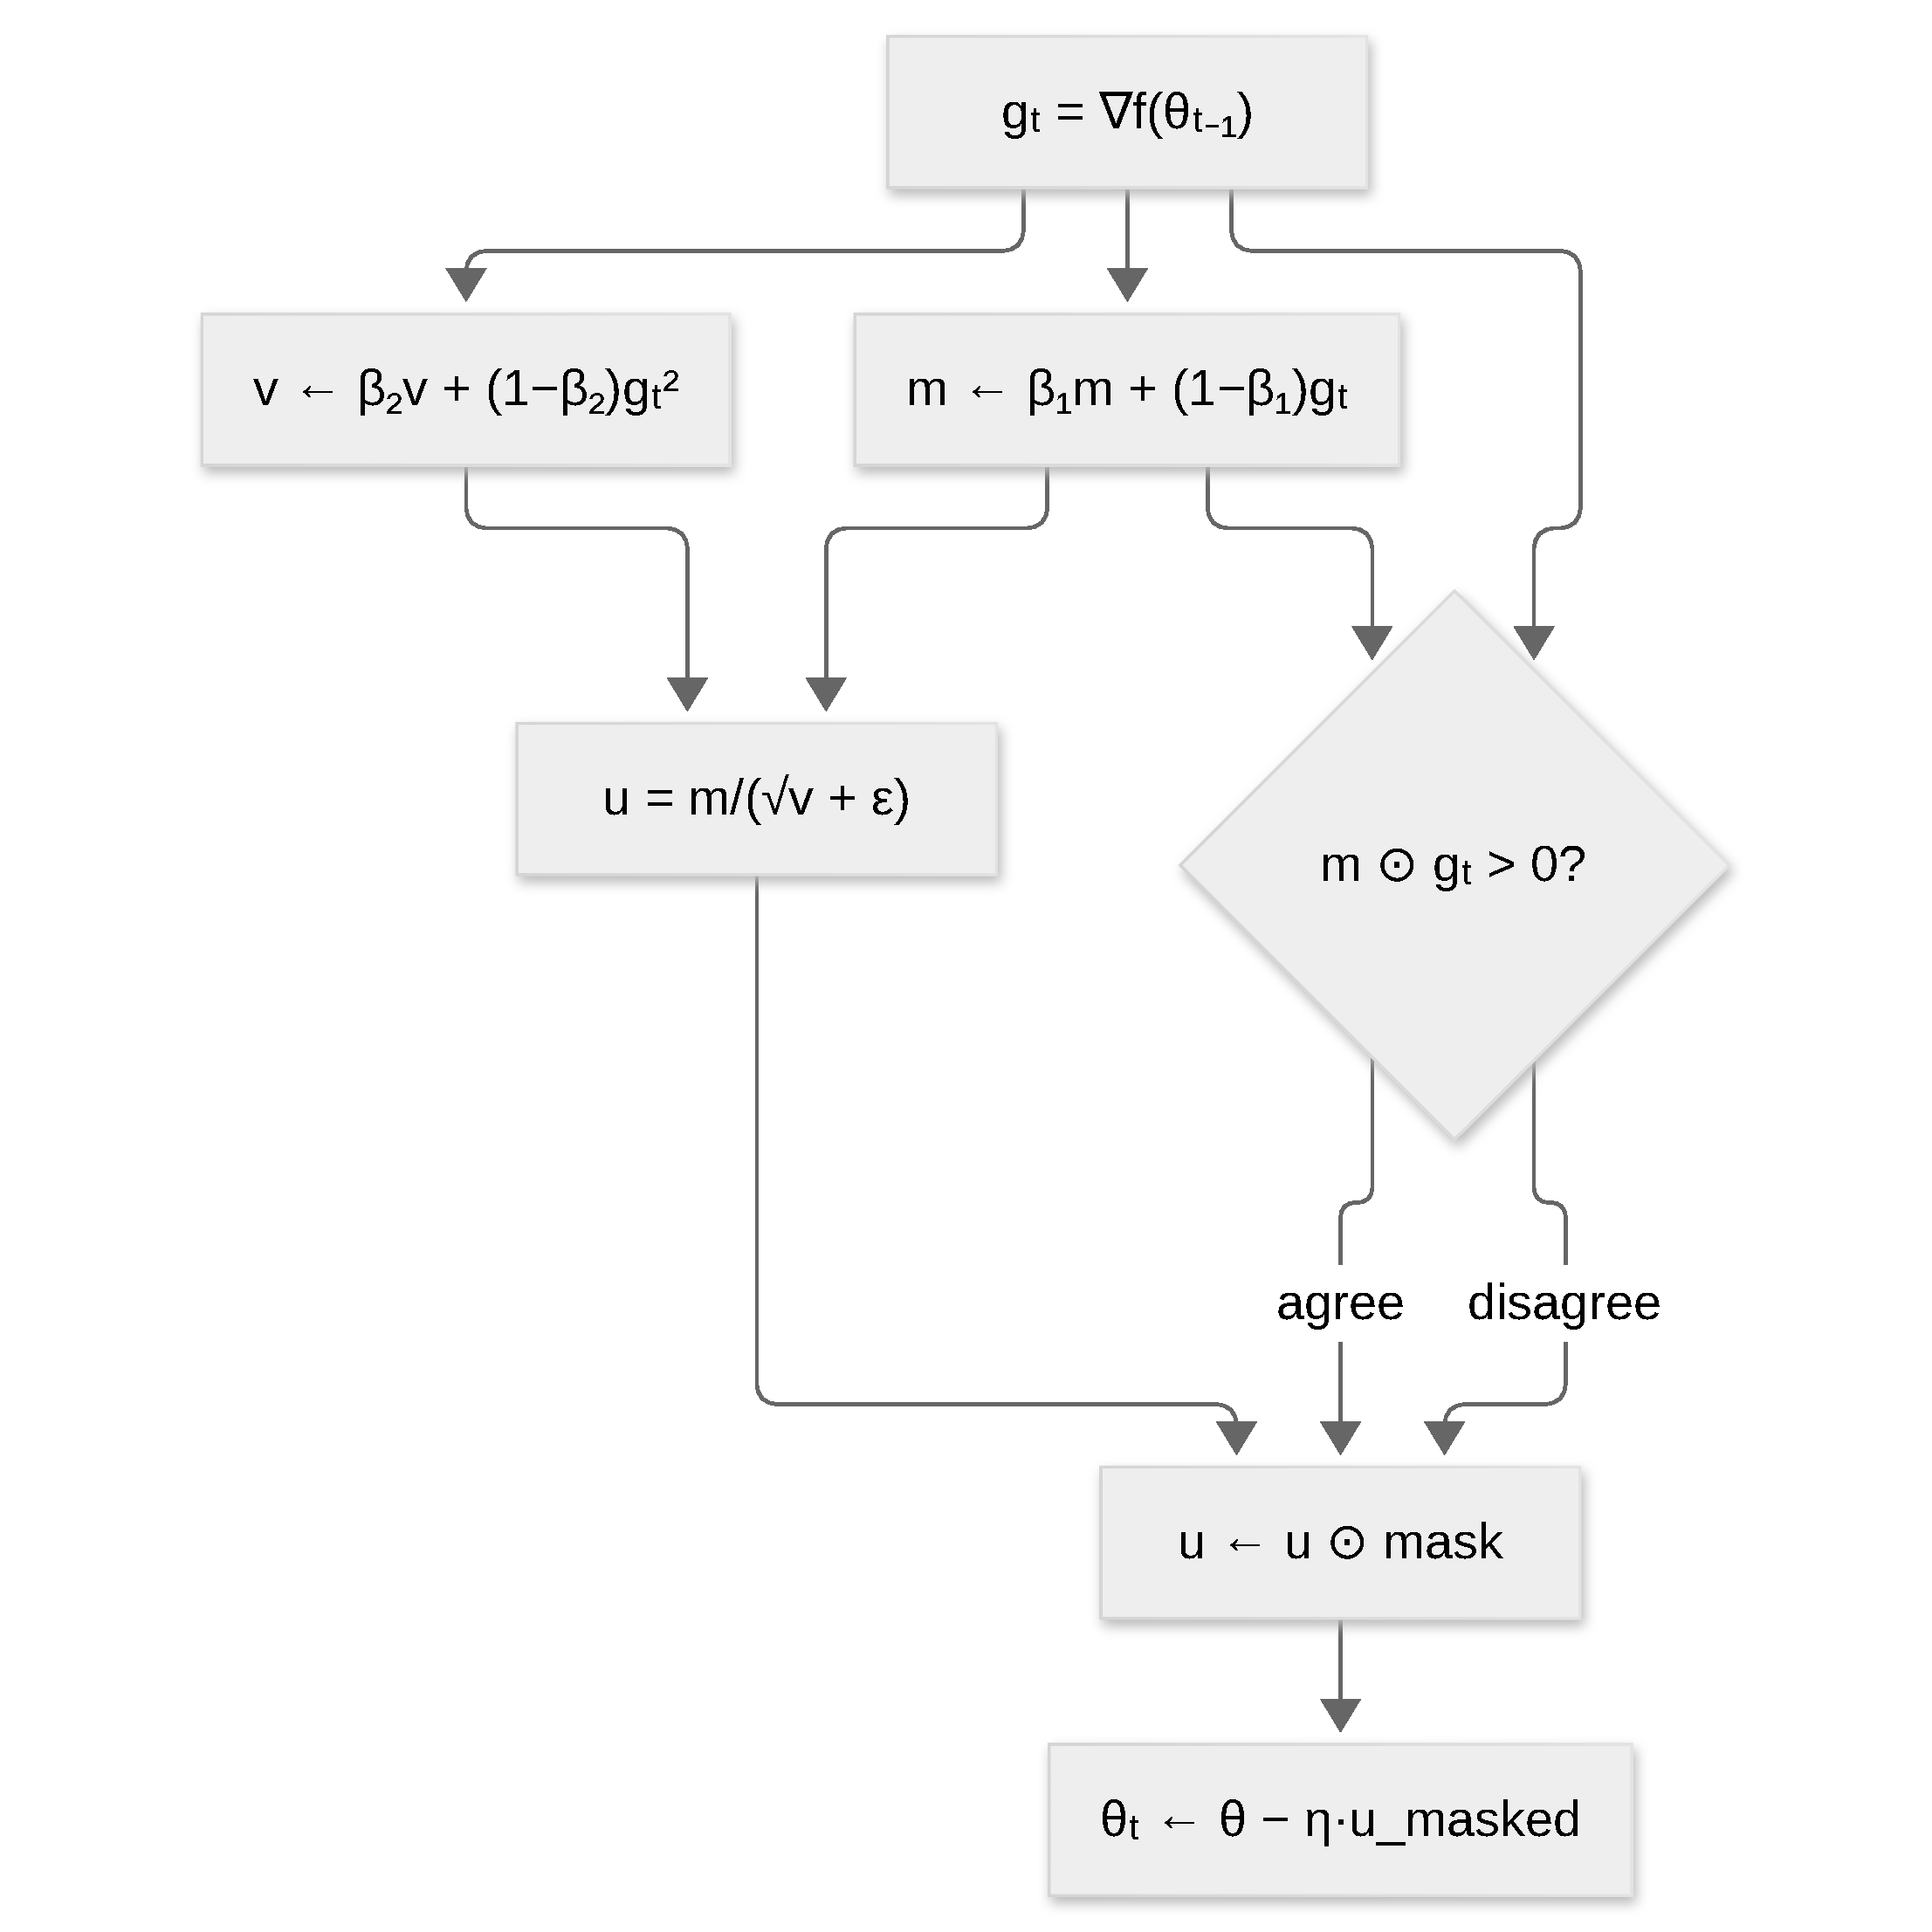
\includegraphics{figures/optimizers/cautious.pdf}}
\caption{Step flow of Cautious AdamW: a consensus mask keeps only update coordinates where momentum and gradient agree.}
\label{fig:opt-cautious}
\end{figure}
The Cautious framework applies a \textbf{one-line modification} to any momentum-based optimizer: mask the update so that only dimensions where momentum and gradient directions agree are applied:
\begin{align}
\text{mask}_i &= \begin{cases} 1 & \text{if } m_t[i] \cdot g_t[i] > 0 \quad\text{(agreement)} \\ 0 & \text{otherwise} \end{cases} \\
u_t &= \left(\frac{m_t}{\sqrt{v_t}+\epsilon}\right) \odot \text{mask} \quad\text{(element-wise masking)} \\
\theta_{t+1} &= \theta_t - \eta u_t
\end{align}
The intuition: momentum $m_t$ estimates the gradient direction from history; the current gradient $g_t$ is instantaneous signal. When both agree, the optimizer is confident and should update aggressively. When they disagree, the optimizer is conflicted---the historical trend points toward a region that may have been good before, but current evidence contradicts it. By masking conflicted dimensions, Cautious becomes more conservative and avoids corrupted steps.

\begin{algorithm}[H]
\caption{Cautious AdamW (Consensus-based Update Masking)}
\label{alg:cautious}
\begin{algorithmic}[1]
\Require Initial parameters $\theta_0$, learning rate $\eta$, $\beta_1, \beta_2$, weight decay $\lambda$
\Ensure Updated parameters $\theta_T$
\State Initialize: $m \gets 0$, $v \gets 0$
\For{$t = 1, 2, \ldots, T$}
    \State $g_t \gets \nabla f(\theta_{t-1})$
    \State $m \gets \beta_1 m + (1-\beta_1) g_t$
    \State $v \gets \beta_2 v + (1-\beta_2) g_t^2$
    \State Consensus mask: $\text{mask}_i \gets 1$ if $m[i] \cdot g_t[i] > 0$, else $0$ \Comment{Agreement}
    \State Base Adam update: $u \gets m / (\sqrt{v} + \epsilon)$
    \State Apply mask: $u_{\text{masked}} \gets u \odot \text{mask}$ \Comment{Element-wise}
    \If{weight\_decay $> 0$}
        \State $\theta_{t-1} \gets \theta_{t-1}(1 - \eta\lambda)$
    \EndIf
    \State $\theta_t \gets \theta_{t-1} - \eta u_{\text{masked}}$
\EndFor
\Return $\theta_T$
\end{algorithmic}
\end{algorithm}

\paragraph{Cons.}
\begin{itemize}[leftmargin=*]
\item Masking can discard useful updates when momentum and gradient temporarily disagree.
\item Requires a base momentum optimizer plus the element-wise mask.
\end{itemize}

\paragraph{Pros.}
\begin{itemize}[leftmargin=*]
\item A one-line modification applicable to any momentum-based optimizer.
\item Up to \textbf{1.47$\times$ speedup} on Llama and MAE pretraining while preserving convergence guarantees.
\end{itemize}

\subsection{Large-Batch, Memory-Efficient, and Parameter-Free Optimizers}
\paragraph{LAMB (Layer-wise Adaptive Moments optimizer for Batch training).}
\begin{figure}[H]
\centering
\fitfigure{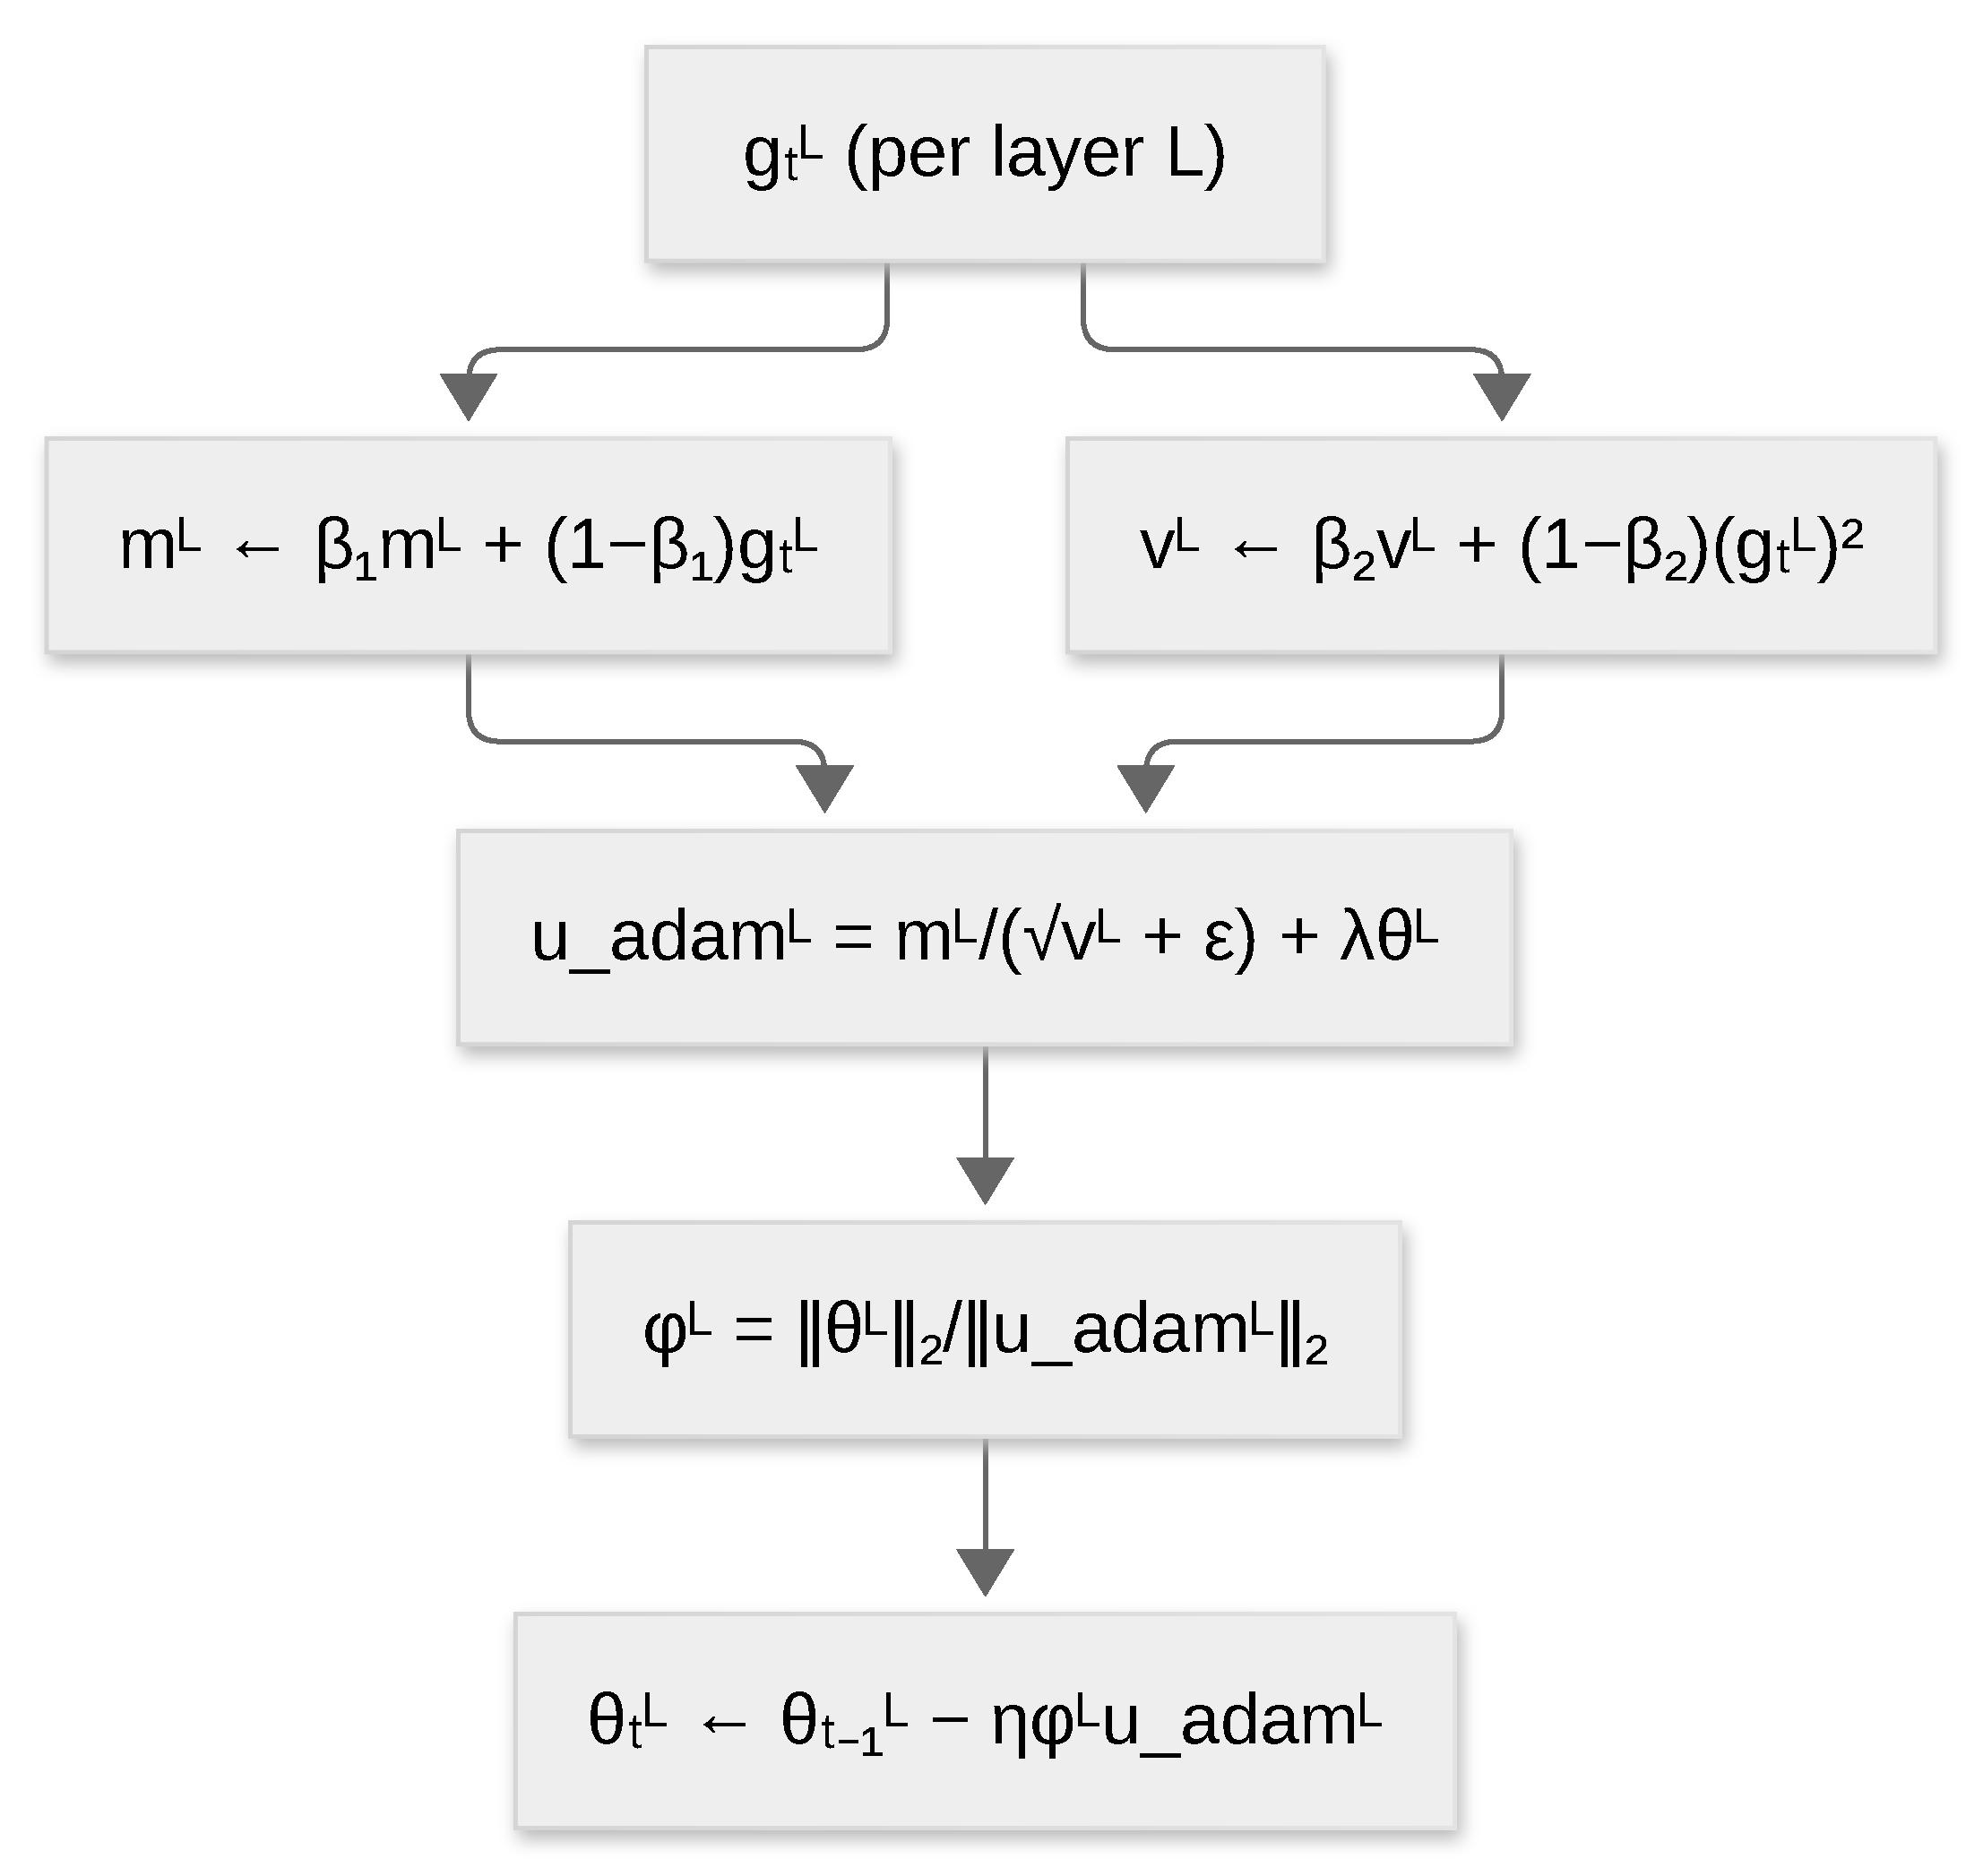
\includegraphics{figures/optimizers/lamb.pdf}}
\caption{Step flow of LAMB: per-layer Adam step rescaled by the trust ratio between weight and update norms.}
\label{fig:opt-lamb}
\end{figure}
LAMB extends Adam with \textbf{layer-wise adaptive rate scaling} (inspired by LARS), enabling stable training with extreme batch sizes (e.g., 64K on BERT):
\begin{align}
m_t^L &= \beta_1 m_{t-1}^L + (1-\beta_1)g_t^L \quad\text{(layer-wise first moment)} \\
v_t^L &= \beta_2 v_{t-1}^L + (1-\beta_2)(g_t^L)^2 \\
u_{\text{adam}}^L &= \frac{m_t^L}{\sqrt{v_t^L}+\epsilon} + \lambda\theta_{t-1}^L \quad\text{(base adaptive step with decay)} \\
\phi^L &= \frac{\|\theta_{t-1}^L\|_2}{\|u_{\text{adam}}^L\|_2} \quad\text{(trust ratio: layer normalization)} \\
\theta_t^L &= \theta_{t-1}^L - \eta \cdot \phi^L \cdot u_{\text{adam}}^L
\end{align}
The \textbf{trust ratio} $\phi^L = \|\theta^L\|_2 / \|u_{\text{adam}}^L\|_2$ normalizes the effective update step relative to weight magnitude. In very large batches, stochastic gradient noise can exceed signal, destabilizing layer-wise learning rates. By scaling updates proportionally to weight norms, LAMB ensures relative changes rather than absolute ones, preventing small confident updates in large vectors from dominating.

\begin{algorithm}[H]
\caption{LAMB (Layer-wise Adaptive Moments optimizer for Batch training)}
\label{alg:lamb}
\begin{algorithmic}[1]
\Require Initial parameters $\theta_0$, learning rate $\eta$, $\beta_1, \beta_2$, weight decay $\lambda$
\Ensure Updated parameters $\theta_T$
\State Initialize: For each layer $L$: $m^L \gets 0$, $v^L \gets 0$
\For{$t = 1, 2, \ldots, T$}
    \For{each layer $L$}
        \State $g_t^L \gets \nabla f(\theta_t^L)$
        \State $m^L \gets \beta_1 m^L + (1-\beta_1) g_t^L$
        \State $v^L \gets \beta_2 v^L + (1-\beta_2) (g_t^L)^2$
        \State Base Adam: $u_{\text{adam}}^L \gets m^L / (\sqrt{v^L} + \epsilon)$
        \If{weight\_decay $> 0$}
            \State $u_{\text{adam}}^L \gets u_{\text{adam}}^L + \lambda \theta_{t-1}^L$
        \EndIf
        \State Trust ratio: $\phi^L \gets \|\theta_{t-1}^L\|_2 / \|u_{\text{adam}}^L\|_2$ if both nonzero, else $1$
        \State $\theta_t^L \gets \theta_{t-1}^L - \eta \phi^L u_{\text{adam}}^L$
    \EndFor
\EndFor
\Return $\theta_T$
\end{algorithmic}
\end{algorithm}

\paragraph{Cons.}
\begin{itemize}[leftmargin=*]
\item Layer-wise norm bookkeeping and trust-ratio computation add per-step overhead.
\item The trust ratio is unstable when layer or update norms are close to zero.
\end{itemize}

\paragraph{Pros.}
\begin{itemize}[leftmargin=*]
\item Enables stable training with extreme batch sizes (e.g., 64K on BERT).
\item Preserves small-batch generalization benefits while scaling the batch.
\end{itemize}

\paragraph{Schedule-Free AdamW.}
\begin{figure}[H]
\centering
\fitfigure{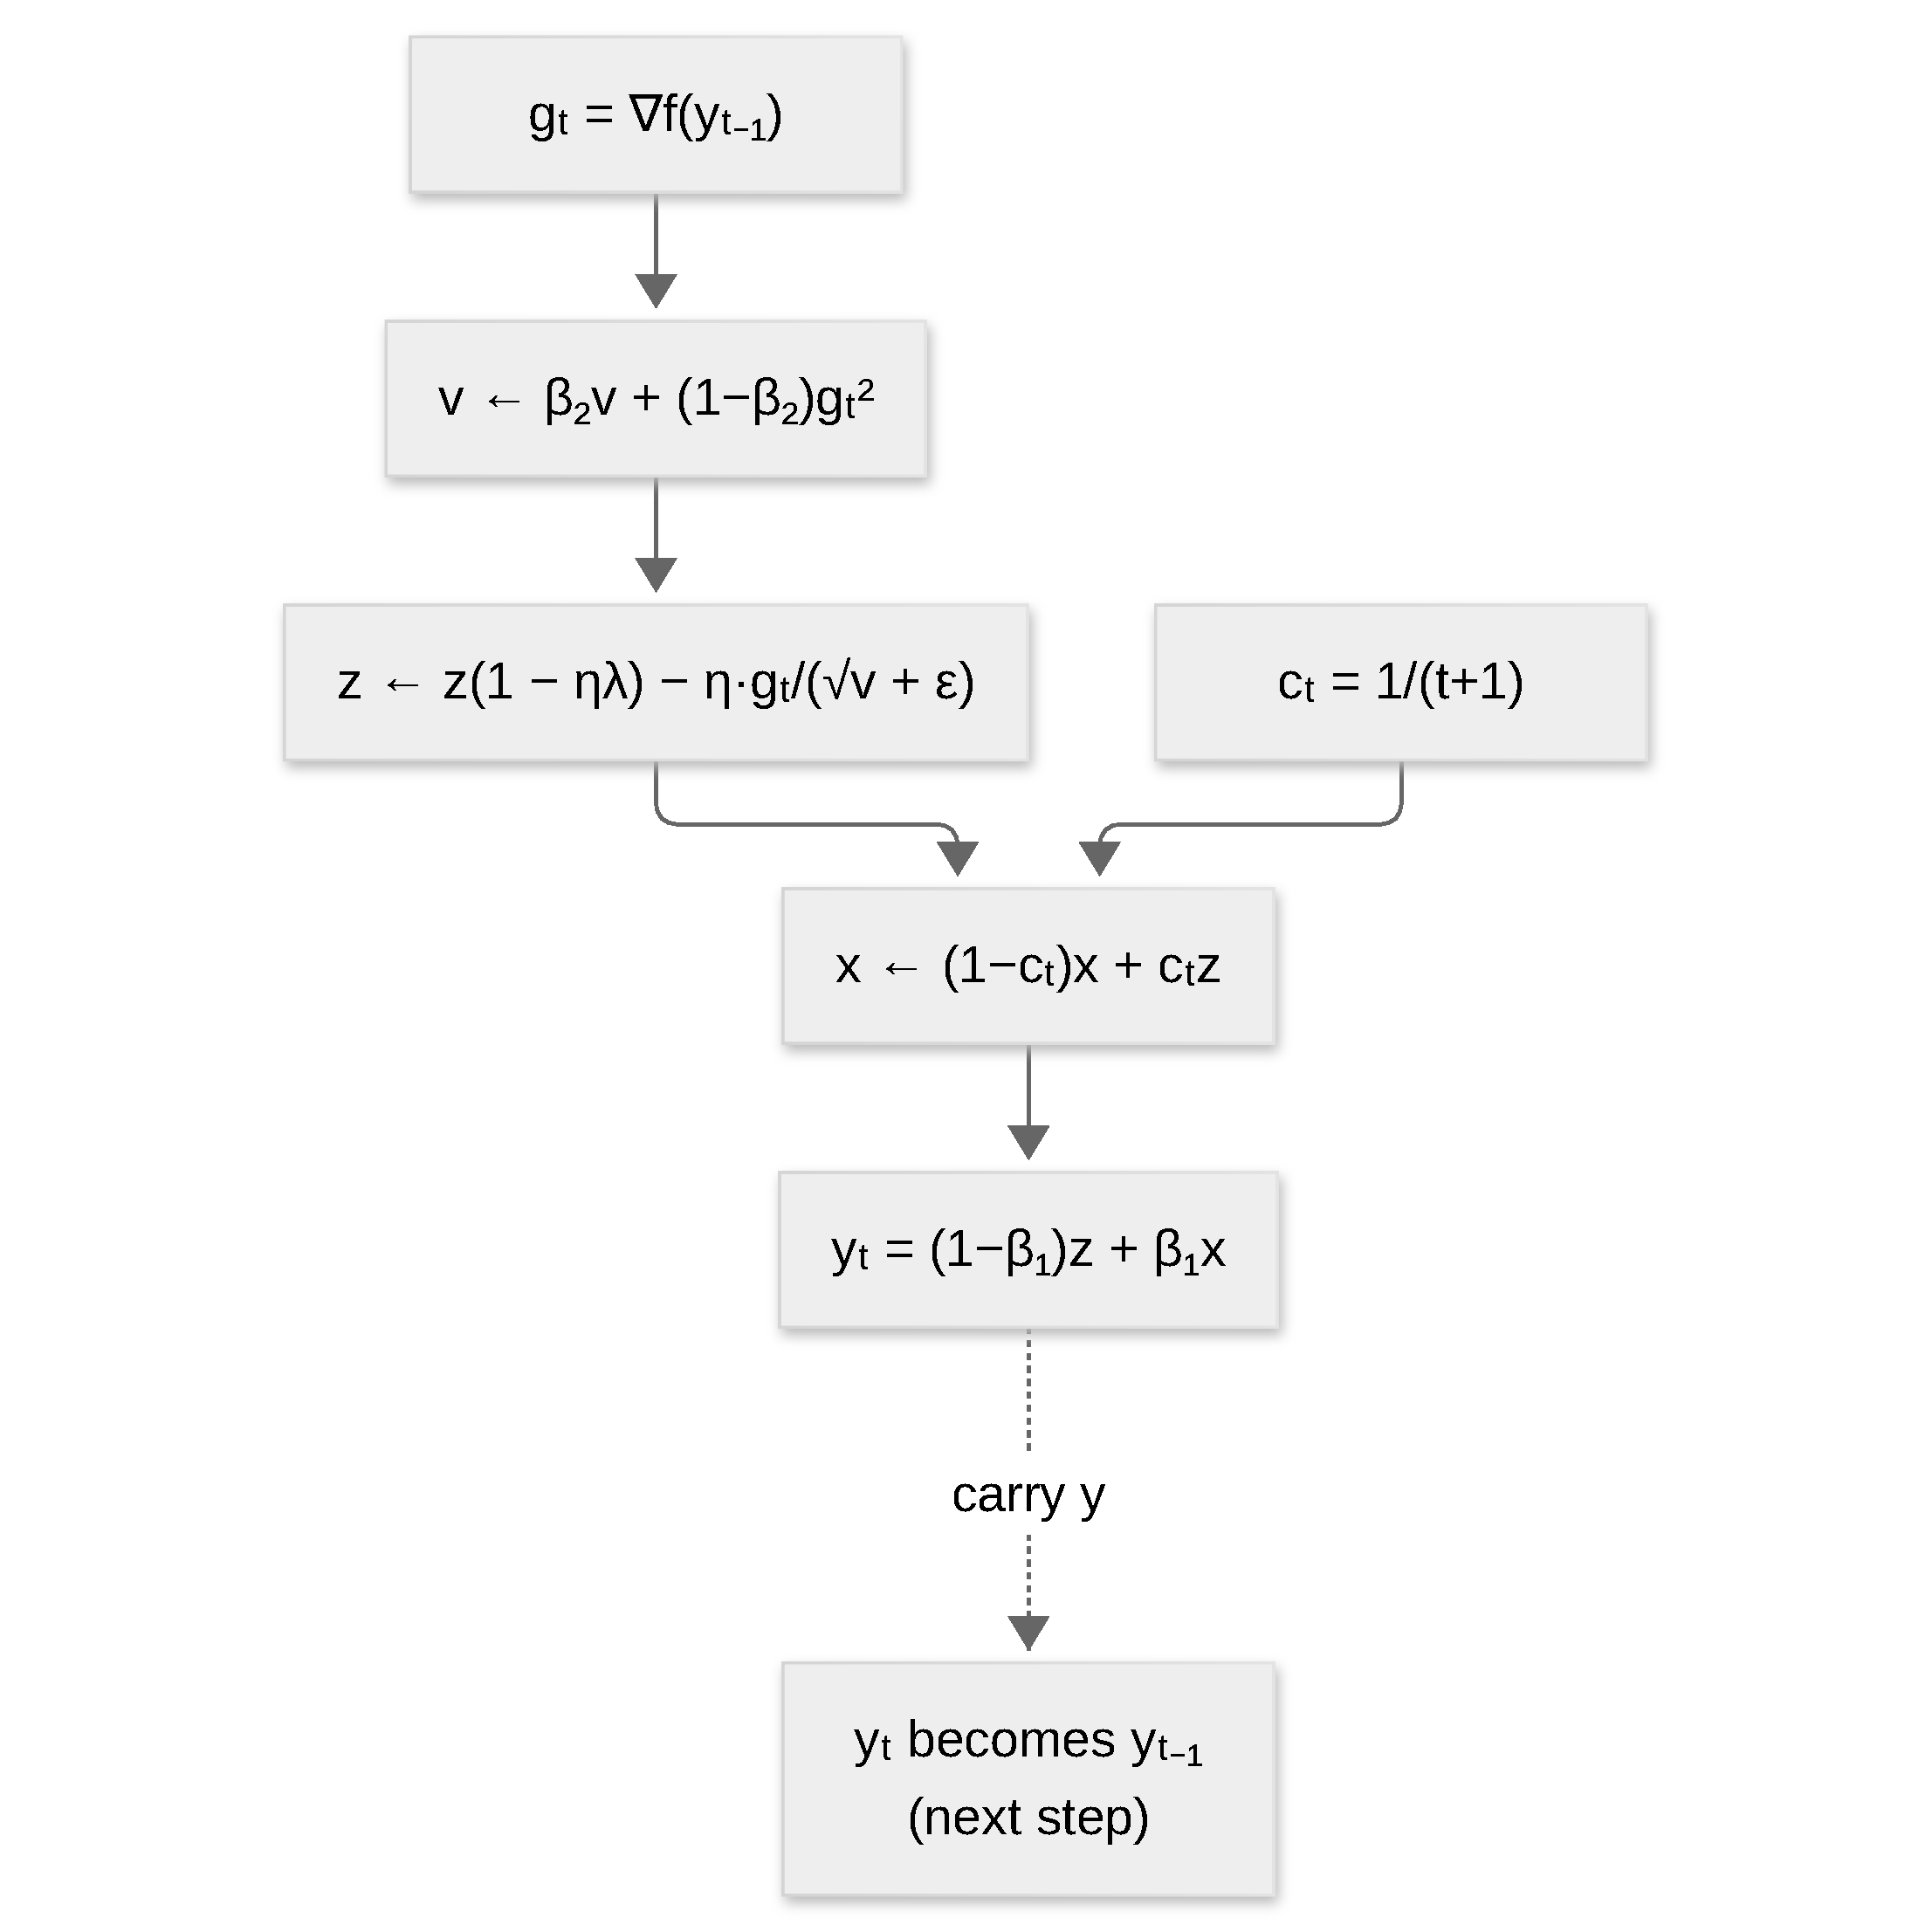
\includegraphics{figures/optimizers/schedulefree.pdf}}
\caption{Step flow of Schedule-Free AdamW: exploration stream $z$, iterate average $x$, and interpolation point $y$, with implicit $1/(t+1)$ averaging.}
\label{fig:opt-schedulefree}
\end{figure}
Schedule-free methods remove explicit scheduler design from the optimization recipe. The algorithm maintains two parameter streams: $z_t$ (exploration) and $x_t$ (smooth average):
\begin{align}
v_t &= \beta_2 v_{t-1} + (1-\beta_2)g_t^2 \quad\text{(variance)} \\
z_t &= z_{t-1}(1-\eta\lambda) - \eta\frac{g_t}{\sqrt{v_t}+\epsilon} \quad\text{(adaptive step with decay)} \\
c_t &= \frac{1}{t+1} \quad\text{(averaging coefficient, decreases over time)} \\
x_t &= (1-c_t)x_{t-1} + c_t z_t \quad\text{(iterate averaging)} \\
y_t &= (1-\beta)z_t + \beta x_t \quad\text{(interpolation for evaluation point)}
\end{align}
The averaging coefficient $c_t = 1/(t+1)$ implements an implicit learning-rate schedule without explicitly specifying total steps $T$. This framework unifies scheduling and iterate averaging: the algorithm explores via $z_t$ while accumulating stable direction via $x_t$. The evaluation point $y_t$ (used for gradient computation) interpolates between exploration and stability.

\begin{algorithm}[H]
\caption{Schedule-Free AdamW}
\label{alg:schedulefree}
\begin{algorithmic}[1]
\Require Initial parameters $\theta_0$, learning rate $\eta$ (fixed), $\beta_1, \beta_2$, weight decay $\lambda$
\Ensure Updated parameters $\theta_T$ or averaging $x_T$
\State Initialize: $z \gets \theta_0$ (exploration), $x \gets \theta_0$ (average), $v \gets 0$, $t \gets 0$
\For{$t = 1, 2, \ldots, T$}
    \State $g_t \gets \nabla f(y_{t-1})$ (gradient at interpolation point)
    \State $v \gets \beta_2 v + (1-\beta_2) g_t^2$ \Comment{Variance}
    \State Weight decay on $z$: $z \gets z(1 - \eta\lambda)$
    \State $z \gets z - \eta g_t / (\sqrt{v} + \epsilon)$ \Comment{Adaptive step on raw}
    \State $c_t \gets 1 / (t+1)$ \Comment{Averaging coefficient}
    \State $x \gets (1-c_t) x + c_t z$ \Comment{Iterate averaging}
    \State $y_t \gets (1-\beta_1) z + \beta_1 x$ \Comment{Interpolation for next eval}
\EndFor
\Return $x_T$ or $y_T$
\end{algorithmic}
\end{algorithm}

\paragraph{Cons.}
\begin{itemize}[leftmargin=*]
\item Maintains two parameter streams ($z$ and $x$) and requires explicit handling of the evaluation point.
\item Behavior departs from scheduled baselines, which complicates comparisons.
\end{itemize}

\paragraph{Pros.}
\begin{itemize}[leftmargin=*]
\item Removes the explicit learning-rate schedule and its total-step hyperparameter.
\item State-of-the-art convergence across convex optimization, large-scale deep learning, and reinforcement learning.
\end{itemize}

\paragraph{Adafactor.}
\begin{figure}[H]
\centering
\fitfigure{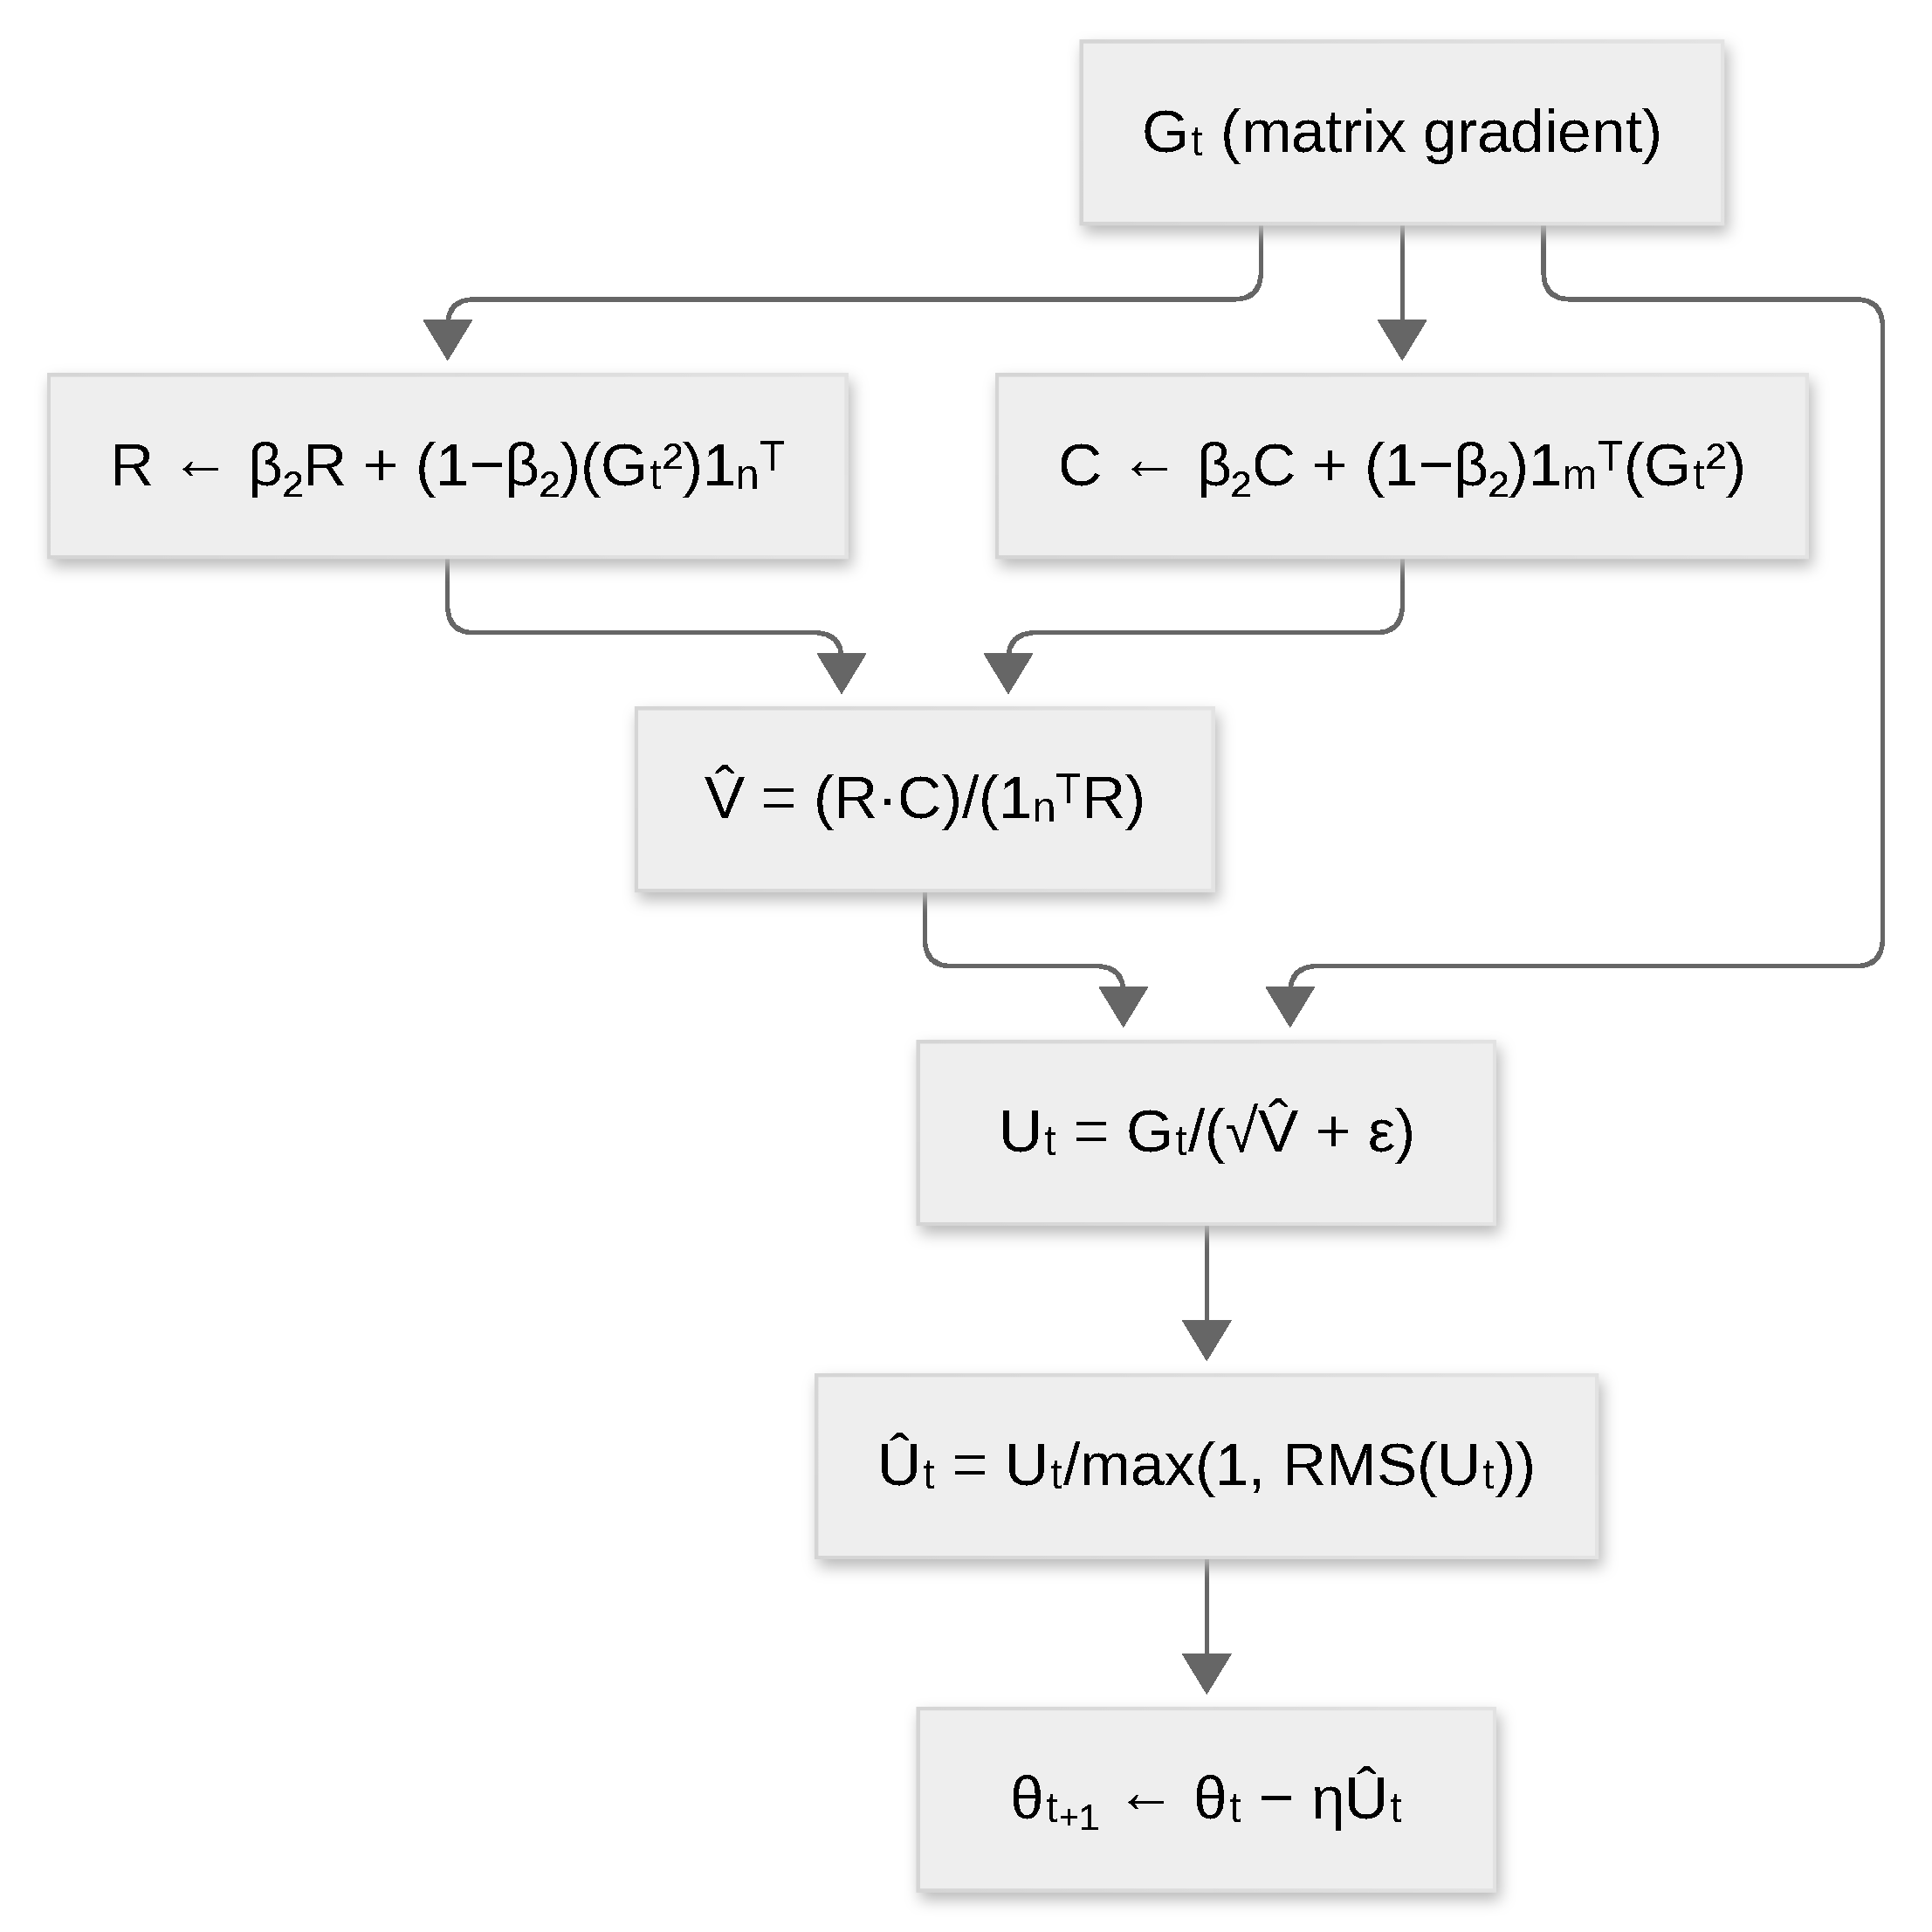
\includegraphics{figures/optimizers/adafactor.pdf}}
\caption{Step flow of Adafactor: factorized row/column second-moment accumulators, outer-product variance reconstruction, and RMS clipping.}
\label{fig:opt-adafactor}
\end{figure}
Adafactor reduces optimizer memory by \textbf{factorizing} second-moment statistics for matrix-shaped parameters, storing only row and column accumulators rather than dense variance states. For a gradient matrix $G_t \in \mathbb{R}^{m \times n}$:
\begin{align}
R_t &= \beta_2 R_{t-1} + (1-\beta_2)(G_t^2) \mathbf{1}_n^T \quad\text{(row variance)} \\
C_t &= \beta_2 C_{t-1} + (1-\beta_2) \mathbf{1}_m^\top (G_t^2) \quad\text{(column variance)} \\
\hat{V}_t &= \frac{R_t C_t}{\mathbf{1}_n^\top R_t} \quad\text{(reconstructed variance via outer product)} \\
U_t &= \frac{G_t}{\sqrt{\hat{V}_t}+\epsilon} \quad\text{(normalized adaptive step)} \\
\hat{U}_t &= \frac{U_t}{\max(1, \text{RMS}(U_t))} \quad\text{(stability clipping)}
\end{align}

\begin{algorithm}[H]
\caption{Adafactor (Factorized Second-Moment Statistics)}
\label{alg:adafactor}
\begin{algorithmic}[1]
\Require Gradient matrix $G_t \in \mathbb{R}^{m \times n}$, learning rate $\eta$, $\beta_2 \approx 0.999$
\Ensure Updated parameters $\theta_T$
\State Initialize: Row accumulators $R \gets \epsilon \mathbf{1}^T_m$, Column $C \gets \epsilon \mathbf{1}_n$
\For{$t = 1, 2, \ldots, T$}
    \State $G_t \gets \nabla f(\theta_t)$ (matrix gradient)
    \State $R \gets \beta_2 R + (1-\beta_2) (G_t^2) \mathbf{1}_n^T$ \Comment{Row inner products}
    \State $C \gets \beta_2 C + (1-\beta_2) \mathbf{1}_m^\top (G_t^2)$ \Comment{Column inner products}
    \State Reconstructed variance: $\hat{V} \gets (R \cdot C) / (\mathbf{1}_n^\top R)$ \Comment{Via outer product}
    \State Normalized adaptive step: $U_t \gets G_t / (\sqrt{\hat{V}} + \epsilon)$
    \State Per-row RMS clipping: $\hat{U}_t \gets U_t / \max(1, \text{RMS}(U_t))$
    \State $\theta_{t+1} \gets \theta_t - \eta \hat{U}_t$
\EndFor
\Return $\theta_T$
\end{algorithmic}
\end{algorithm}

\paragraph{Cons.}
\begin{itemize}[leftmargin=*]
\item Factorized variance is an approximation and can be unstable on some tasks.
\item Reduced optimization expressiveness relative to full Adam.
\end{itemize}

\paragraph{Pros.}
\begin{itemize}[leftmargin=*]
\item Memory drops from $O(n_{\text{params}})$ to $O(\sqrt{n_{\text{params}}})$ for matrix parameters.
\item Most attractive when VRAM is dominated by optimizer state rather than activations.
\end{itemize}

\paragraph{GaLore (Gradient Low-Rank Projection).}
\begin{figure}[H]
\centering
\fitfigure{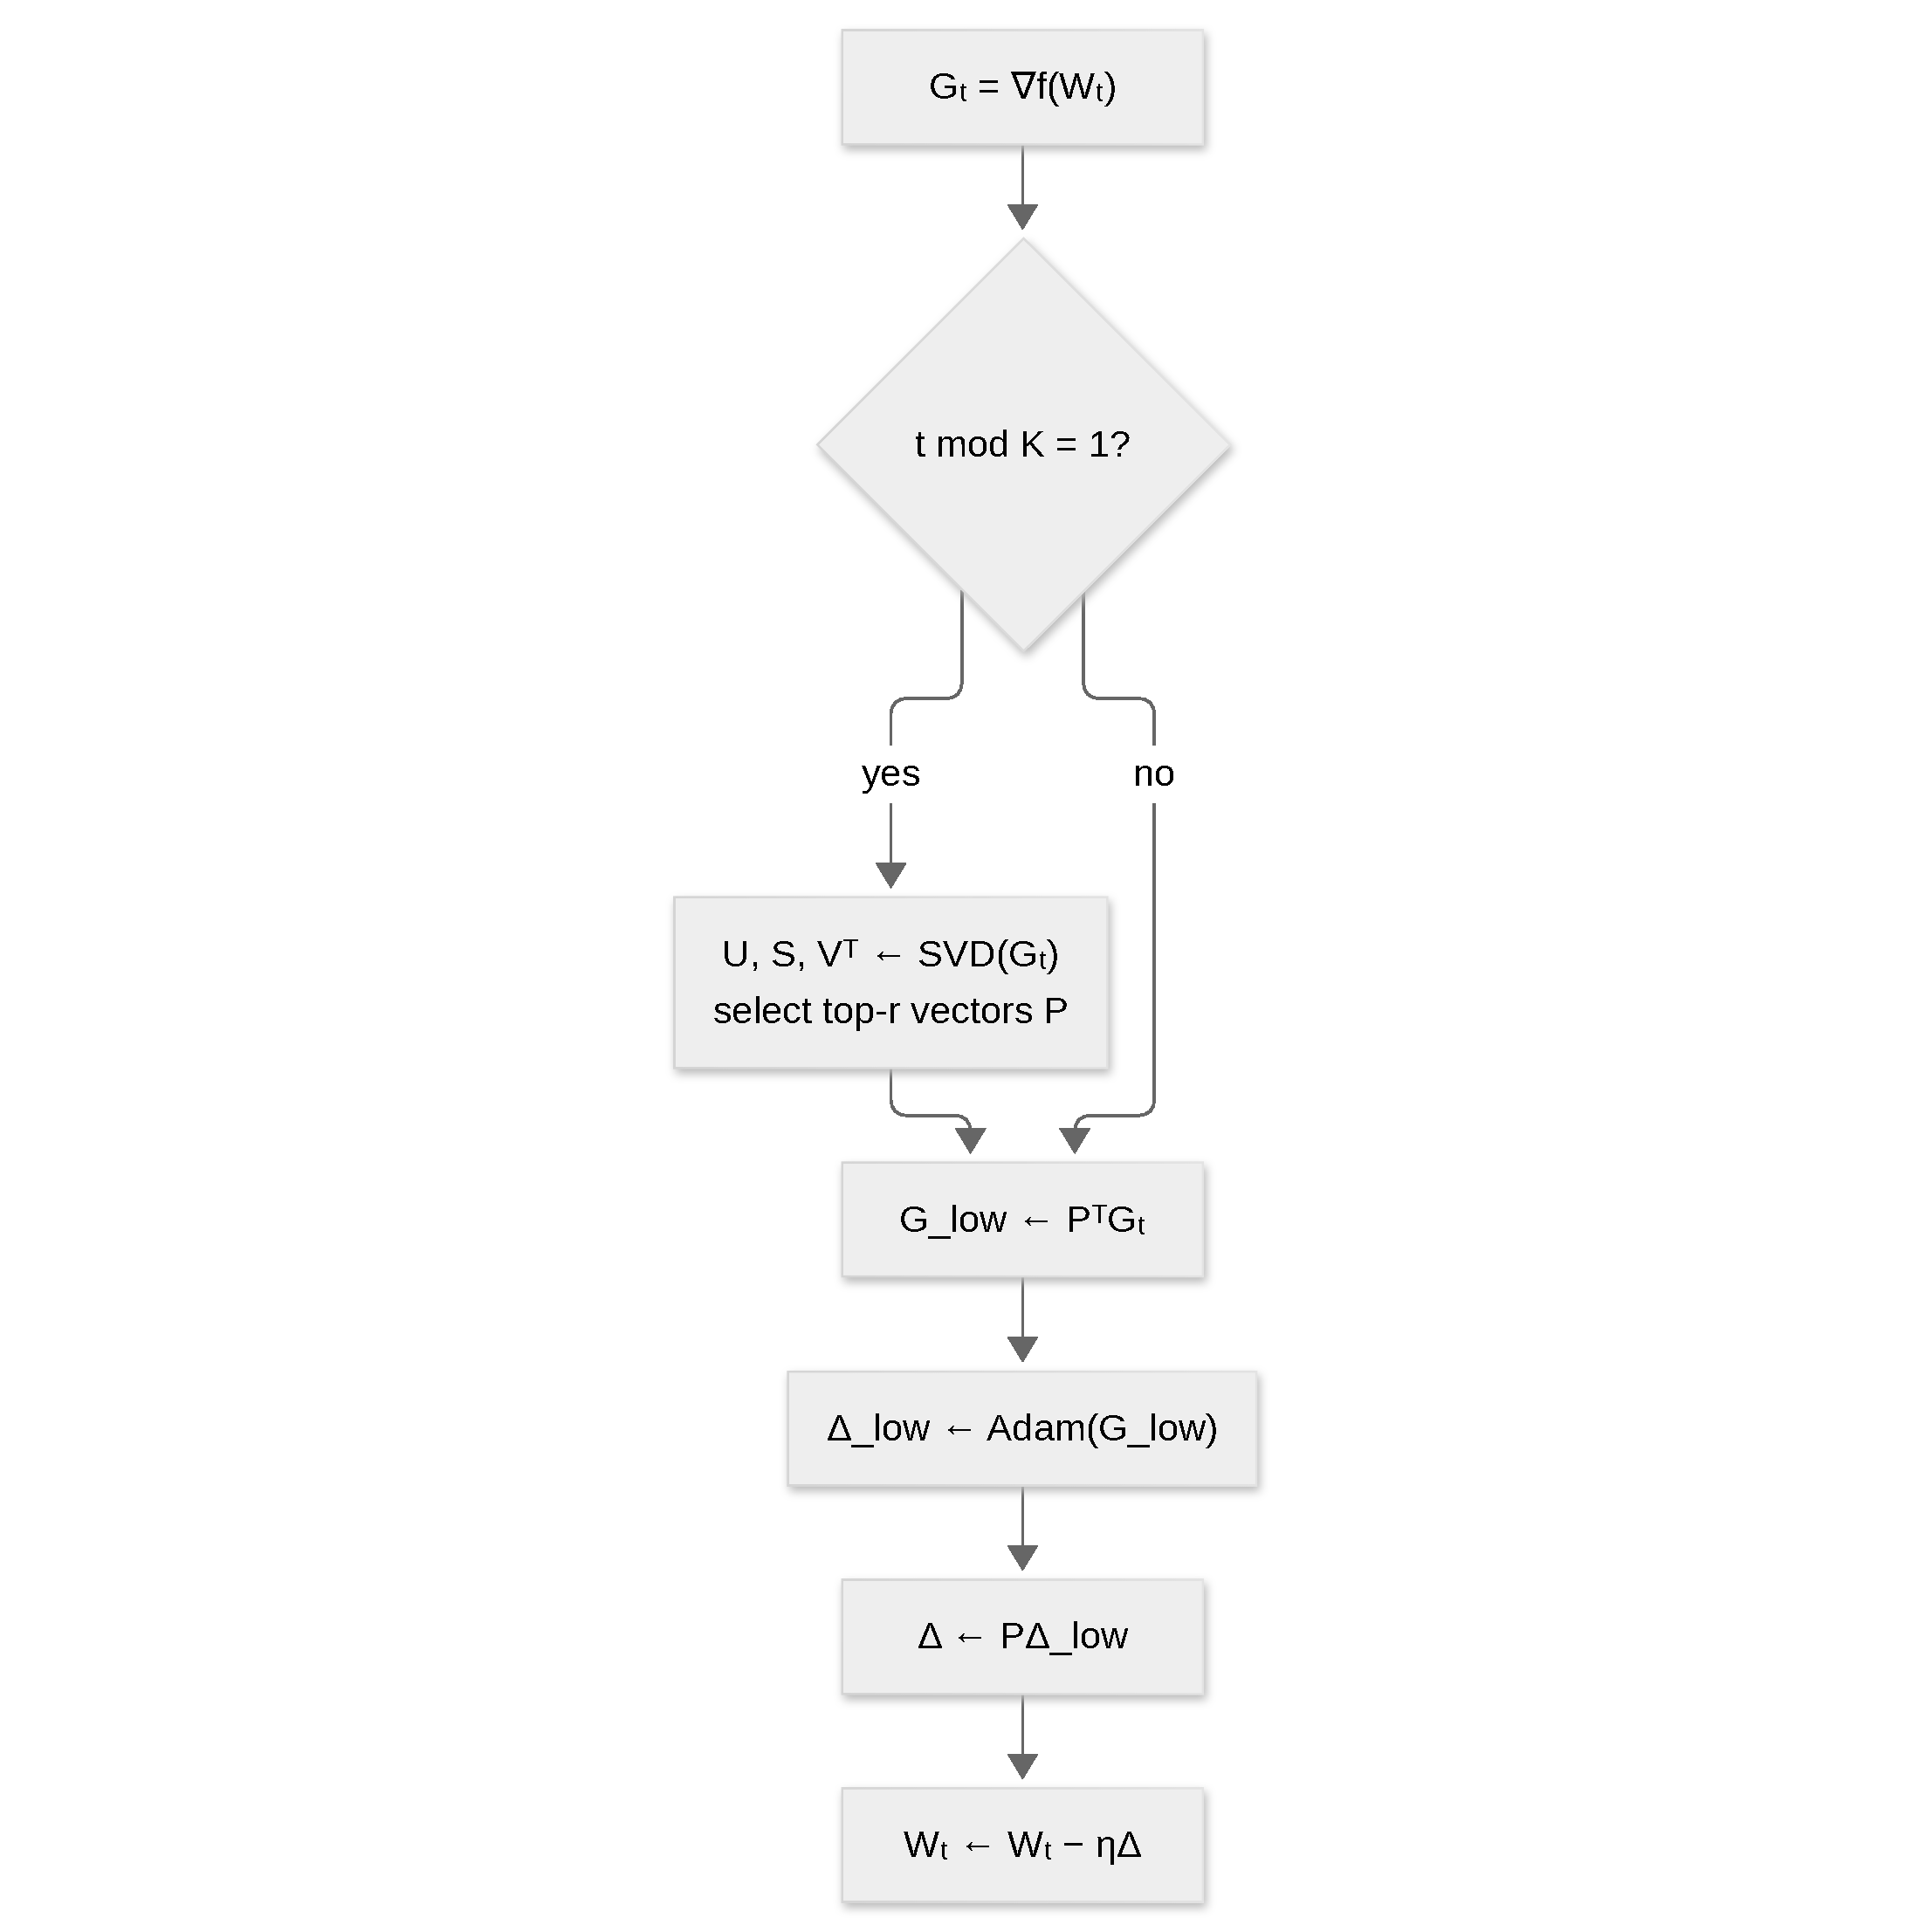
\includegraphics{figures/optimizers/galore.pdf}}
\caption{Step flow of GaLore: periodic SVD projection of the gradient into a low-rank subspace, Adam in that subspace, and reconstruction.}
\label{fig:opt-galore}
\end{figure}
GaLore projects 2D gradients into a low-rank subspace before optimization, reducing optimizer-state memory while maintaining adaptive step scaling. For a 2D parameter matrix $W \in \mathbb{R}^{m \times n}$:
\begin{align}
U, S, V &= \text{SVD}(G_t) \quad\text{(compute singular decomposition)} \\
P &\in \mathbb{R}^{n \times r} \quad\text{or} \quad P^\top \in \mathbb{R}^{r \times m} \quad\text{(select top-$r$ singular vectors)} \\
G_{\text{low}} &= P^\top G_t \quad\text{(project to low-rank space)} \\
\Delta_{\text{low}} &= \text{Adam}(G_{\text{low}}) \quad\text{(optimize in compressed space)} \\
\Delta &= P \Delta_{\text{low}} \quad\text{(reconstruct in original space)}
\end{align}
By projecting into a rank-$r$ subspace (typically $r \ll \min(m,n)$), optimizer state is reduced from $O(mn)$ to $O(r(m+n))$ for 2D parameters. This complementary memory-saving approach is especially relevant when the model is too large for full-rank optimizer state.

\begin{algorithm}[H]
\caption{GaLore (Gradient Low-Rank Projection)}
\label{alg:galore}
\begin{algorithmic}[1]
\Require 2D parameter matrix $W \in \mathbb{R}^{m \times n}$, learning rate $\eta$, rank $r \ll \min(m,n)$
\Ensure Updated parameters $\theta_T$
\State Initialize: Adam state in low-rank space (if rank-2 variant)
\For{$t = 1, 2, \ldots, T$}
    \State $G_t \gets \nabla f(W_t)$
    \If{$t \mod K = 1$}  \Comment{Periodic SVD}
        \State $U_t, S_t, V_t^\top \gets \text{SVD}(G_t)$ (full or thin)
        \State Select projection: $P \gets U_t[:, :r]$ or $P \gets V_t[:, :r]$
    \EndIf
    \State Project gradient: $G_{\text{low}} \gets P^\top G_t$ (or $G_t P^\top$ for right projection)
    \State Run Adam on low-rank: $\Delta_{\text{low}} \gets \text{Adam}(G_{\text{low}})$
    \State Reconstruct in original space: $\Delta \gets P \Delta_{\text{low}}$ (or $\Delta_{\text{low}} P^\top$)
    \State $W_t \gets W_t - \eta \Delta$
\EndFor
\Return $\theta_T$
\end{algorithmic}
\end{algorithm}

\paragraph{Cons.}
\begin{itemize}[leftmargin=*]
\item Periodic SVD adds compute and introduces a projection-refresh interval to tune.
\item Low-rank projection can discard gradient information.
\end{itemize}

\paragraph{Pros.}
\begin{itemize}[leftmargin=*]
\item Optimizer state reduced from $O(mn)$ to $O(r(m+n))$ for 2D parameters.
\item Works synergistically with other techniques and has shown strong results on billion-parameter models.
\end{itemize}

\paragraph{APOLLO, APOLLO-Mini, and Q-APOLLO.}
\begin{figure}[H]
\centering
\fitfigure{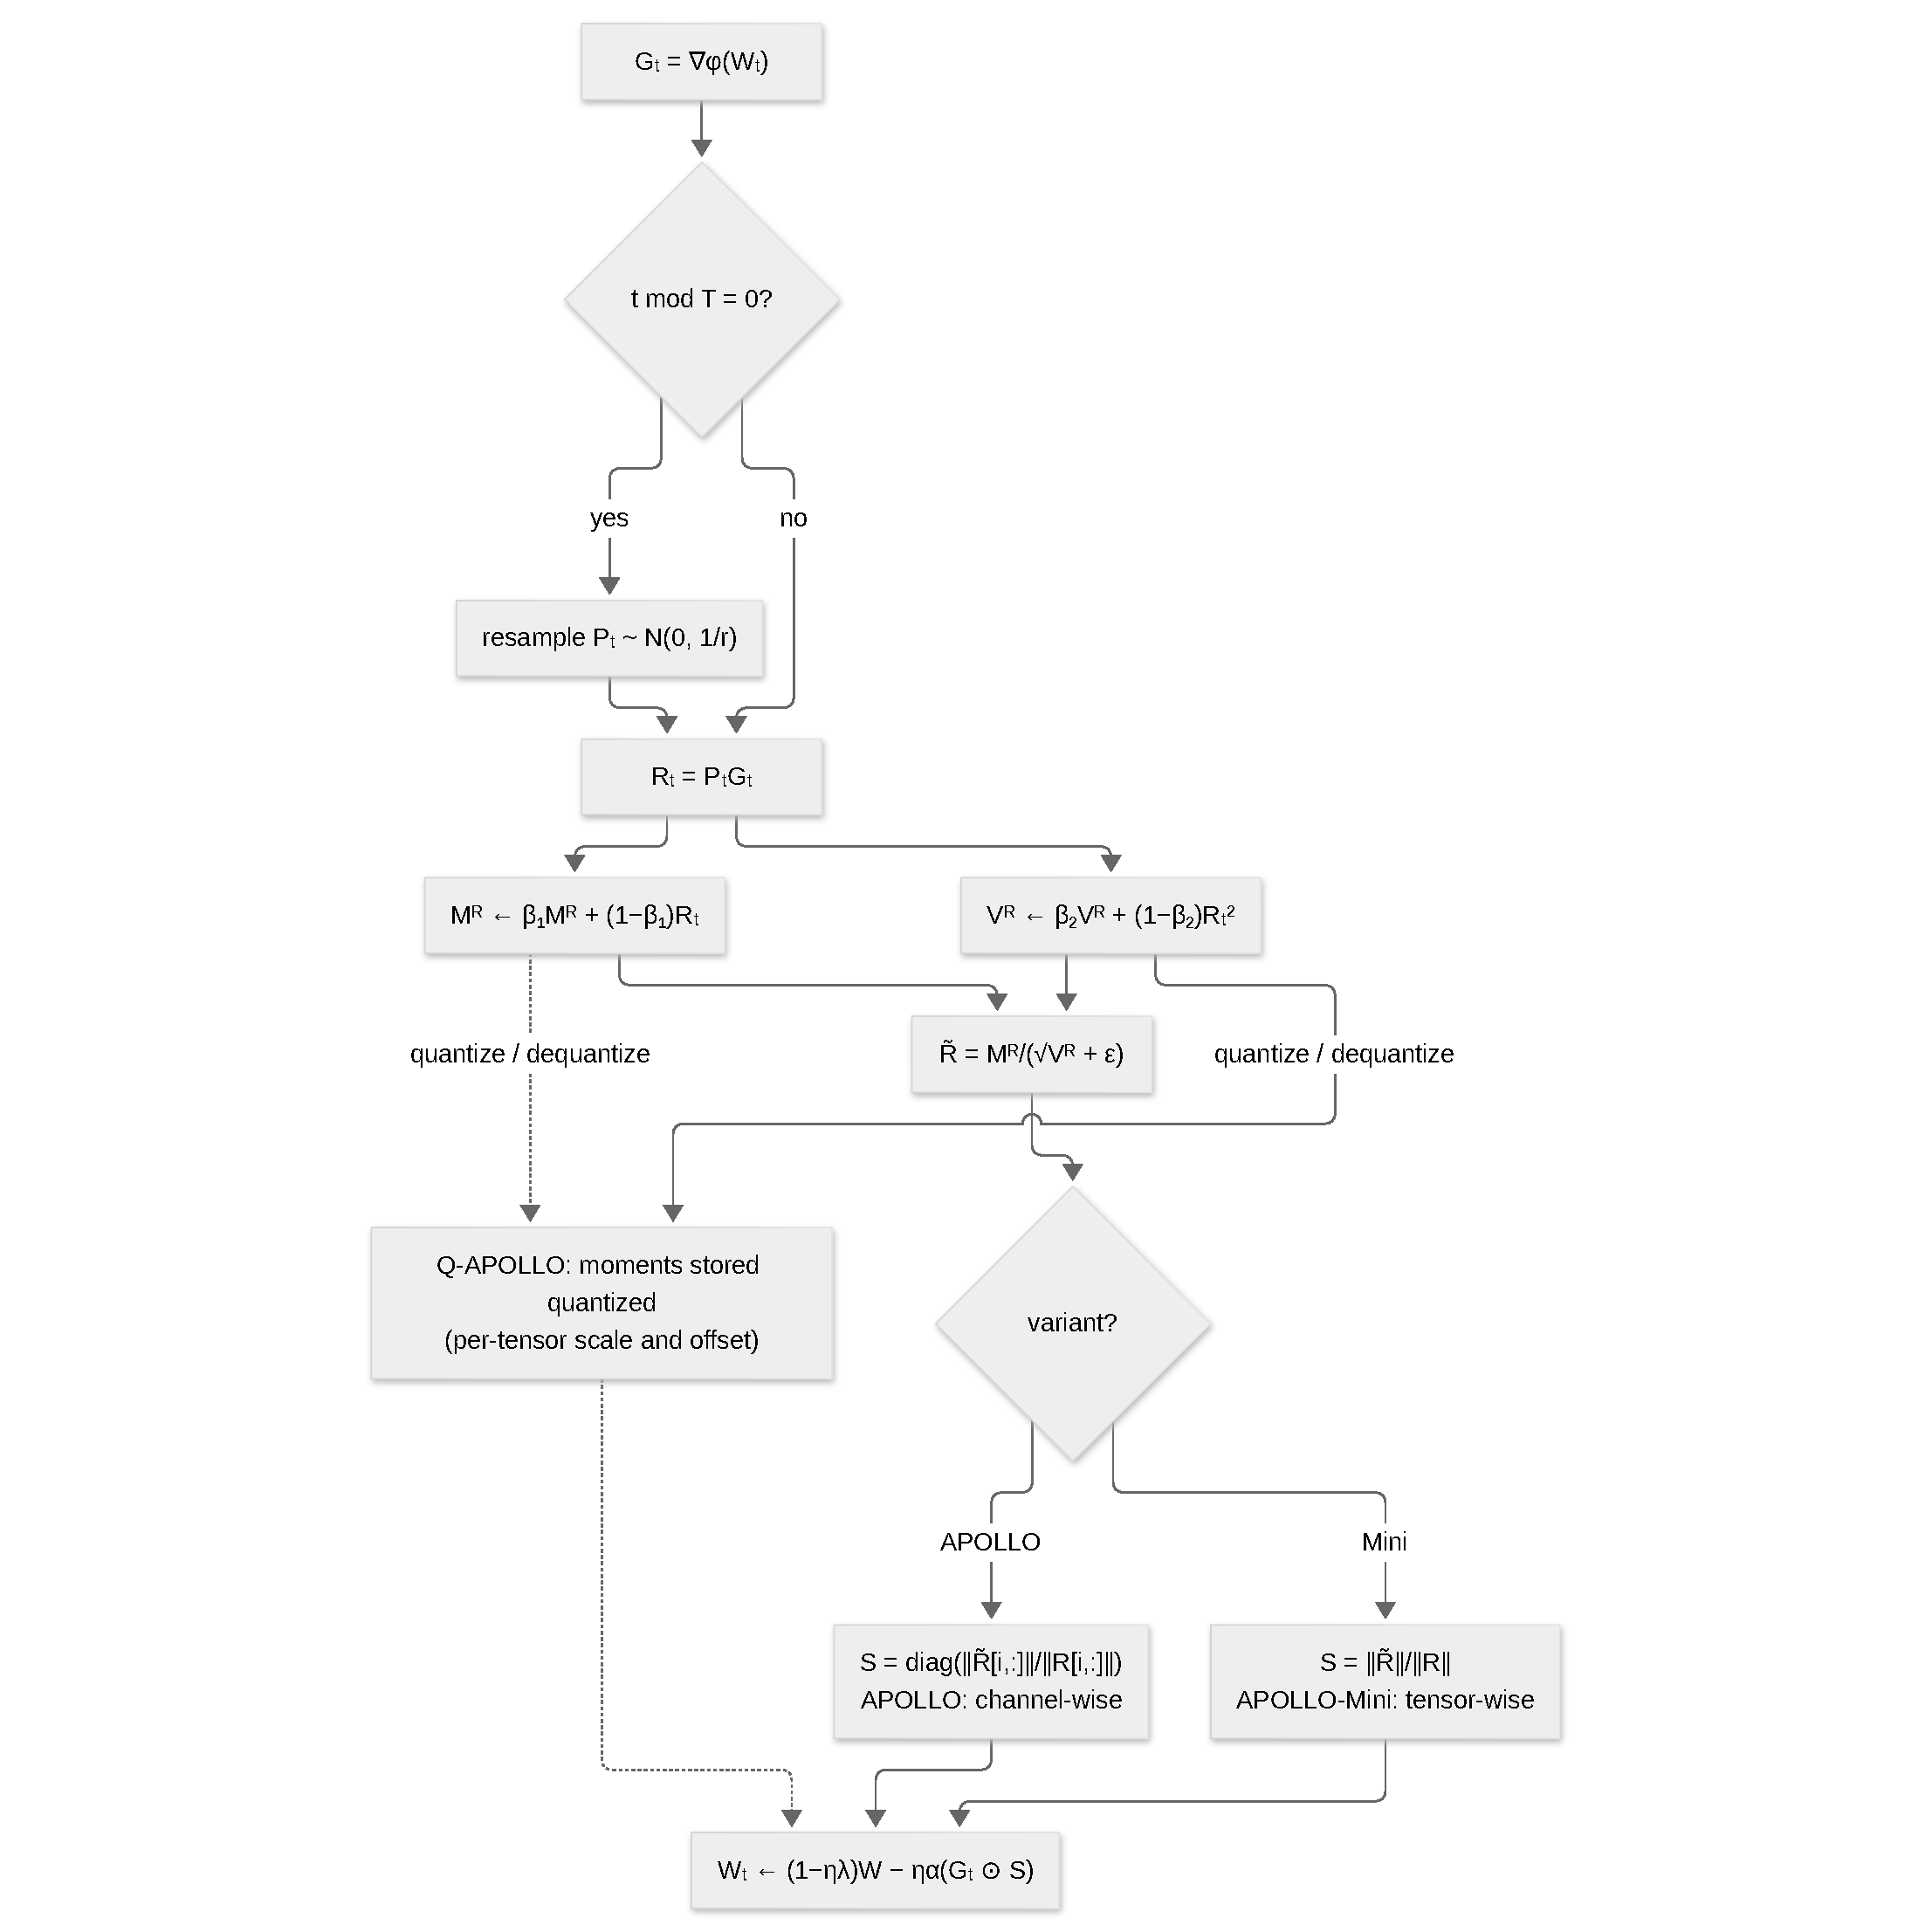
\includegraphics{figures/optimizers/apollo.pdf}}
\caption{Step flow of the APOLLO family: Gaussian-projected moments, structured gradient scaling (channel-wise for APOLLO, scalar for APOLLO-Mini), and quantized state for Q-APOLLO.}
\label{fig:opt-apollo}
\end{figure}
The APOLLO family \citep{zhu2025apollosgdlikememoryadamwlevel} begins from the observation that AdamW's element-wise denominator can be \textbf{coarsened into a structured learning-rate update}. Rather than storing dense moments for every parameter entry, APOLLO projects a matrix gradient $G_t \in \mathbb{R}^{m \times n}$ into a compact random subspace and tracks Adam-style moments there:
\begin{align}
R_t &= P_t G_t \quad\text{or}\quad R_t = G_t P_t^\top \\
M_t^R &= \beta_1 M_{t-1}^R + (1-\beta_1)R_t \\
V_t^R &= \beta_2 V_{t-1}^R + (1-\beta_2)R_t^2 \\
\widetilde{R}_t &= \frac{M_t^R}{\sqrt{V_t^R}+\epsilon}
\end{align}
The projected state is \emph{not} expanded back into a dense low-rank update as in SVD-based methods. Instead, APOLLO estimates a structured scaling tensor $S_t$ in the original space. In the standard APOLLO variant, that scaling is \textbf{channel-wise}: each row or channel receives its own norm ratio. In APOLLO-Mini, the scaling is reduced to a single \textbf{tensor-wise} scalar, corresponding to the rank-1 extreme described in the paper. The resulting parameter update is therefore Adam-like in adaptation but much closer to SGD in state cost:
\[
W_t \gets (1-\eta\lambda)W_{t-1} - \eta\,\alpha\,(G_t \odot S_t)
\]
where $\alpha$ is the extra scale factor used to stabilize highly compressed variants.

\begin{algorithm}[H]
\caption{APOLLO / APOLLO-Mini Structured Gradient Scaling}
\label{alg:apollo-family}
\begin{algorithmic}[1]
\Require Weight matrix $W \in \mathbb{R}^{m \times n}$ with $m \le n$, learning rate $\eta$, scale factor $\alpha$, decay rates $(\beta_1, \beta_2)$, weight decay $\lambda$, rank $r$, projection refresh interval $T$
\Ensure Updated parameters $W_T$
\State Initialize projected moments: $M^R \gets 0$, $V^R \gets 0$, step $t \gets 0$
\Repeat
    \State Compute gradient: $G_t \gets \nabla_W \phi(W_t)$
    \If{$t \bmod T = 0$}
        \State Sample Gaussian projector $P_t \sim \mathcal{N}(0, 1/r)$ with a fresh seed
    \EndIf
    \State Project gradient: $R_t \gets P_t G_t$ \Comment{or $G_t P_t^\top$ depending on layout}
    \State Update projected AdamW moments: $M_t^R, V_t^R \gets \text{AdamWState}(R_t; \beta_1, \beta_2)$
    \State Normalize projected state: $\widetilde{R}_t \gets M_t^R / (\sqrt{V_t^R}+\epsilon)$
    \If{APOLLO}
        \State $S_t \gets \operatorname{diag}(s_1^R, \ldots, s_m^R)$, where $s_i^R = \|\widetilde{R}_t[i,:]\|_2 / \|R_t[i,:]\|_2$
    \Else
        \State $S_t \gets s_t^R$, where $s_t^R = \|\widetilde{R}_t\|_2 / \|R_t\|_2$
    \EndIf
    \State Update weights: $W_t \gets (1-\eta\lambda)W_{t-1} - \eta\,\alpha\,(G_t \odot S_t)$
    \State $t \gets t+1$
\Until{convergence}
\end{algorithmic}
\end{algorithm}

\paragraph{Cons.}
\begin{itemize}[leftmargin=*]
\item Structured scaling is a coarser approximation of AdamW's element-wise denominator.
\item Projectors must be refreshed periodically, and very small ranks make the scaling noisy.
\end{itemize}

\paragraph{Pros.}
\begin{itemize}[leftmargin=*]
\item Replaces repeated SVD with periodically refreshed Gaussian random projection, so the systems cost is ordinary matrix multiplication rather than spectral decomposition.
\item Unusually tolerant to extreme compression: even APOLLO-Mini, which keeps only rank-1 auxiliary state, remains competitive with or better than AdamW while approaching SGD-level memory.
\end{itemize}

\paragraph{APOLLO-Mini.}
APOLLO-Mini is the family member optimized for \textbf{extreme memory efficiency}. The paper motivates it by arguing that, in a rank-1 compact space, channel-wise scaling becomes too noisy, so the update is coarsened further to a single tensor-wise scale. The loss of granularity is partially offset by the explicit scaling factor $\alpha$ (the paper discusses values such as $128$ in this regime), giving a useful point on the optimization Pareto frontier: very small state, no SVD overhead, and still strong pre-training behavior.

\paragraph{Cons.}
\begin{itemize}[leftmargin=*]
\item A single tensor-wise scale loses channel granularity, and rank-1 state can be noisy.
\item Depends on the extra scale factor $\alpha$ (e.g., $128$) to remain stable.
\end{itemize}

\paragraph{Pros.}
\begin{itemize}[leftmargin=*]
\item Smallest state in the APOLLO family, with no SVD overhead.
\item Strong pre-training behavior at near-SGD memory cost.
\end{itemize}

\paragraph{Q-APOLLO.}
The APOLLO paper also stresses that the family combines naturally with \textbf{quantization} for ultra-low-memory training. This repository turns that systems observation into a concrete optimizer variant, \texttt{q\_apollo}. In the implementation, APOLLO's low-rank first and second moments are stored in quantized form together with per-tensor scales and offsets, and are dequantized only when needed for the next step. Q-APOLLO therefore preserves APOLLO's projected-gradient logic while reducing the precision of the remaining optimizer state.

\paragraph{Cons.}
\begin{itemize}[leftmargin=*]
\item Quantized moments introduce approximation error and dequantization overhead.
\item Requires managing per-tensor scales and offsets.
\end{itemize}

\paragraph{Pros.}
\begin{itemize}[leftmargin=*]
\item Reduces the remaining optimizer state to ultra-low precision.
\item Most aggressive memory-saving member of the local optimizer stack while preserving APOLLO's projected-gradient logic.
\end{itemize}

\paragraph{Anon (Adaptivity Non-restricted Optimizer with Novel convergence technique).}
\begin{figure}[H]
\centering
\fitfigure{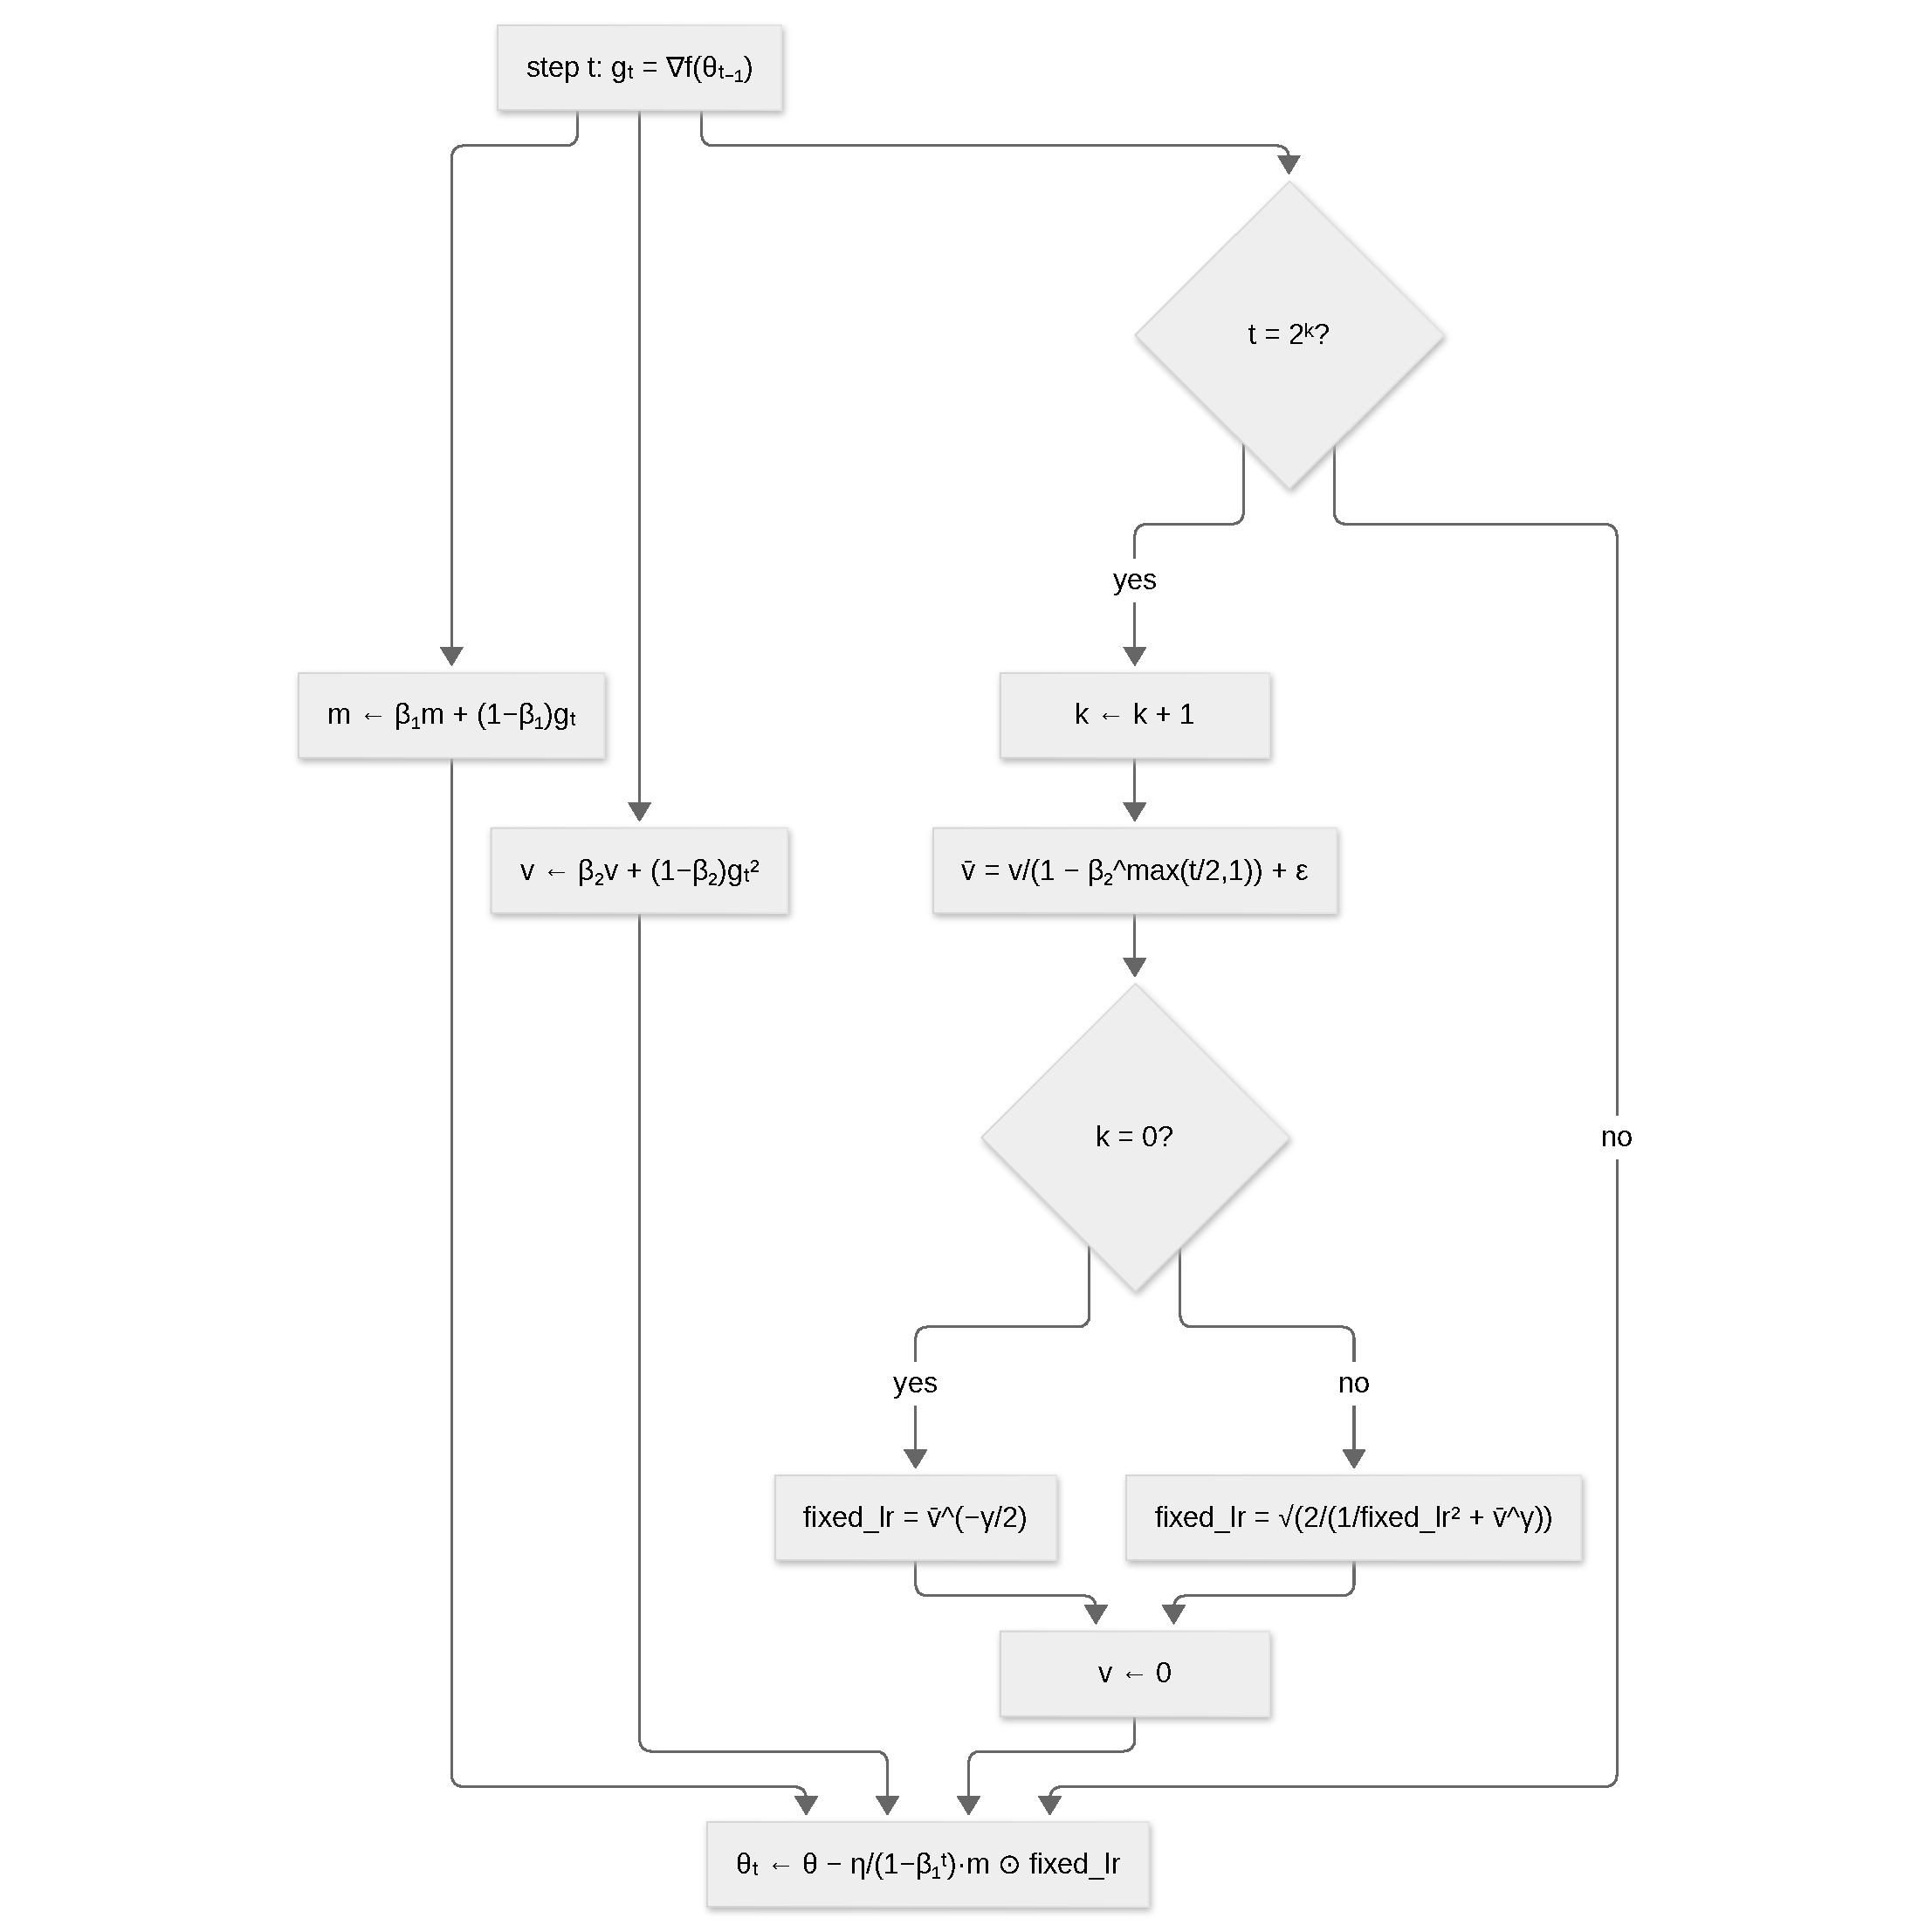
\includegraphics{figures/optimizers/anon.pdf}}
\caption{Step flow of Anon: the IDU preconditioner refreshed at powers of two, with tunable adaptivity $\gamma$ and a bias-corrected momentum update.}
\label{fig:opt-anon}
\end{figure}
Anon \citep{anon2026anon} introduces continuously tunable adaptivity via a single parameter $\gamma \in \mathbb{R}$, bridging the gap between SGD-like ($\gamma=0$) and Adam-like ($\gamma=1$) behaviors, and extrapolating beyond both. The core innovation is the Incremental Delay Update (IDU) mechanism, which enables stable convergence across the entire real-valued adaptivity spectrum:

\begin{align}
m_t &= \beta_1 m_{t-1} + (1-\beta_1) g_t \quad\text{(first moment)}\\
v_t &= \beta_2 v_{t-1} + (1-\beta_2) g_t^2 \quad\text{(second moment)}\\
\bar{v}_t &= \frac{v_t}{1-\beta_2^{\max(t,1)}} + \epsilon \quad\text{(bias-corrected second moment)}\\
\text{fixed\_lr}_k &= \begin{cases}
\bar{v}_k^{-\gamma/2} & \text{if } k = 0 \\
\sqrt{2 / \left(\frac{1}{\text{fixed\_lr}_{k-1}^2} + \bar{v}_k^\gamma\right)} & \text{if } k > 0
\end{cases}\\
\theta_{t+1} &= \theta_t - \frac{\eta}{1-\beta_1^t} \cdot m_t \odot \text{fixed\_lr}_{\lfloor\log_2 t\rfloor}
\end{align}

Unlike standard adaptive optimizers, IDU updates the preconditioner only at powers of two ($t = 2^k$), accumulating gradient statistics between updates and aggregating them recursively. This soft, multi-scale accumulator avoids the hard max-tracking of AMSGrad while provably stabilizing convergence for any $\gamma \in \mathbb{R}$. The parameter $\gamma$ directly controls adaptivity: $\gamma > 1$ accelerates escape from saddle points (favorable for complex architectures), $\gamma = 1$ recovers Adam-like behavior, $\gamma = 0$ yields SGD-like scaling, and $\gamma < 0$ biases toward flatter minima (beneficial for classical architectures like CNNs).

\begin{algorithm}[H]
\caption{Anon (Adaptivity Non-restricted Optimizer with IDU)}
\label{alg:anon}
\begin{algorithmic}[1]
\Require Initial parameters $\theta_0$, learning rate $\eta$, $\beta_1, \beta_2$, tolerance $\epsilon$, adaptivity $\gamma \in \mathbb{R}$
\Ensure Updated parameters $\theta_T$
\State Initialize: $m \gets 0$, $v \gets 0$, fixed\_lr $\gets 0$, step $t \gets 0$, IDU counter $k \gets -1$
\For{$t = 1, 2, \ldots, T$}
    \State $g_t \gets \nabla f(\theta_{t-1})$
    \State $m \gets \beta_1 m + (1-\beta_1) g_t$
    \State $v \gets \beta_2 v + (1-\beta_2) g_t^2$
    \If{$t = 2^k$}
        \State $k \gets k+1$
        \State $\bar{v} \gets v/(1 - \beta_2^{\max(t/2,1)}) + \epsilon$
        \If{$k = 0$}
            \State fixed\_lr $\gets \bar{v}^{-\gamma/2}$
        \Else
            \State fixed\_lr $\gets \sqrt{2 / (1/\text{fixed\_lr}^2 + \bar{v}^\gamma)}$
        \EndIf
        \State $v \gets 0$
    \EndIf
    \State $\theta_t \gets \theta_{t-1} - \frac{\eta}{1-\beta_1^t} \cdot m \odot \text{fixed\_lr}$
\EndFor
\Return $\theta_T$
\end{algorithmic}
\end{algorithm}

\paragraph{Cons.}
\begin{itemize}[leftmargin=*]
\item Maintains three state buffers ($m$, $v$, fixed\_lr) and refreshes the preconditioner on a logarithmic schedule.
\item The adaptivity parameter $\gamma$ must be selected per architecture.
\end{itemize}

\paragraph{Pros.}
\begin{itemize}[leftmargin=*]
\item Same $\mathcal{O}(n)$ per-step complexity class as AdamW, with continuously tunable adaptivity.
\item IDU provably attains $\mathcal{O}(\sqrt{T})$ regret for convex problems and $\mathcal{O}(\ln T / \sqrt{T})$ for non-convex settings.
\end{itemize}

\paragraph{Prodigy (Approximating the Distance Estimate).}
\begin{figure}[H]
\centering
\fitfigure{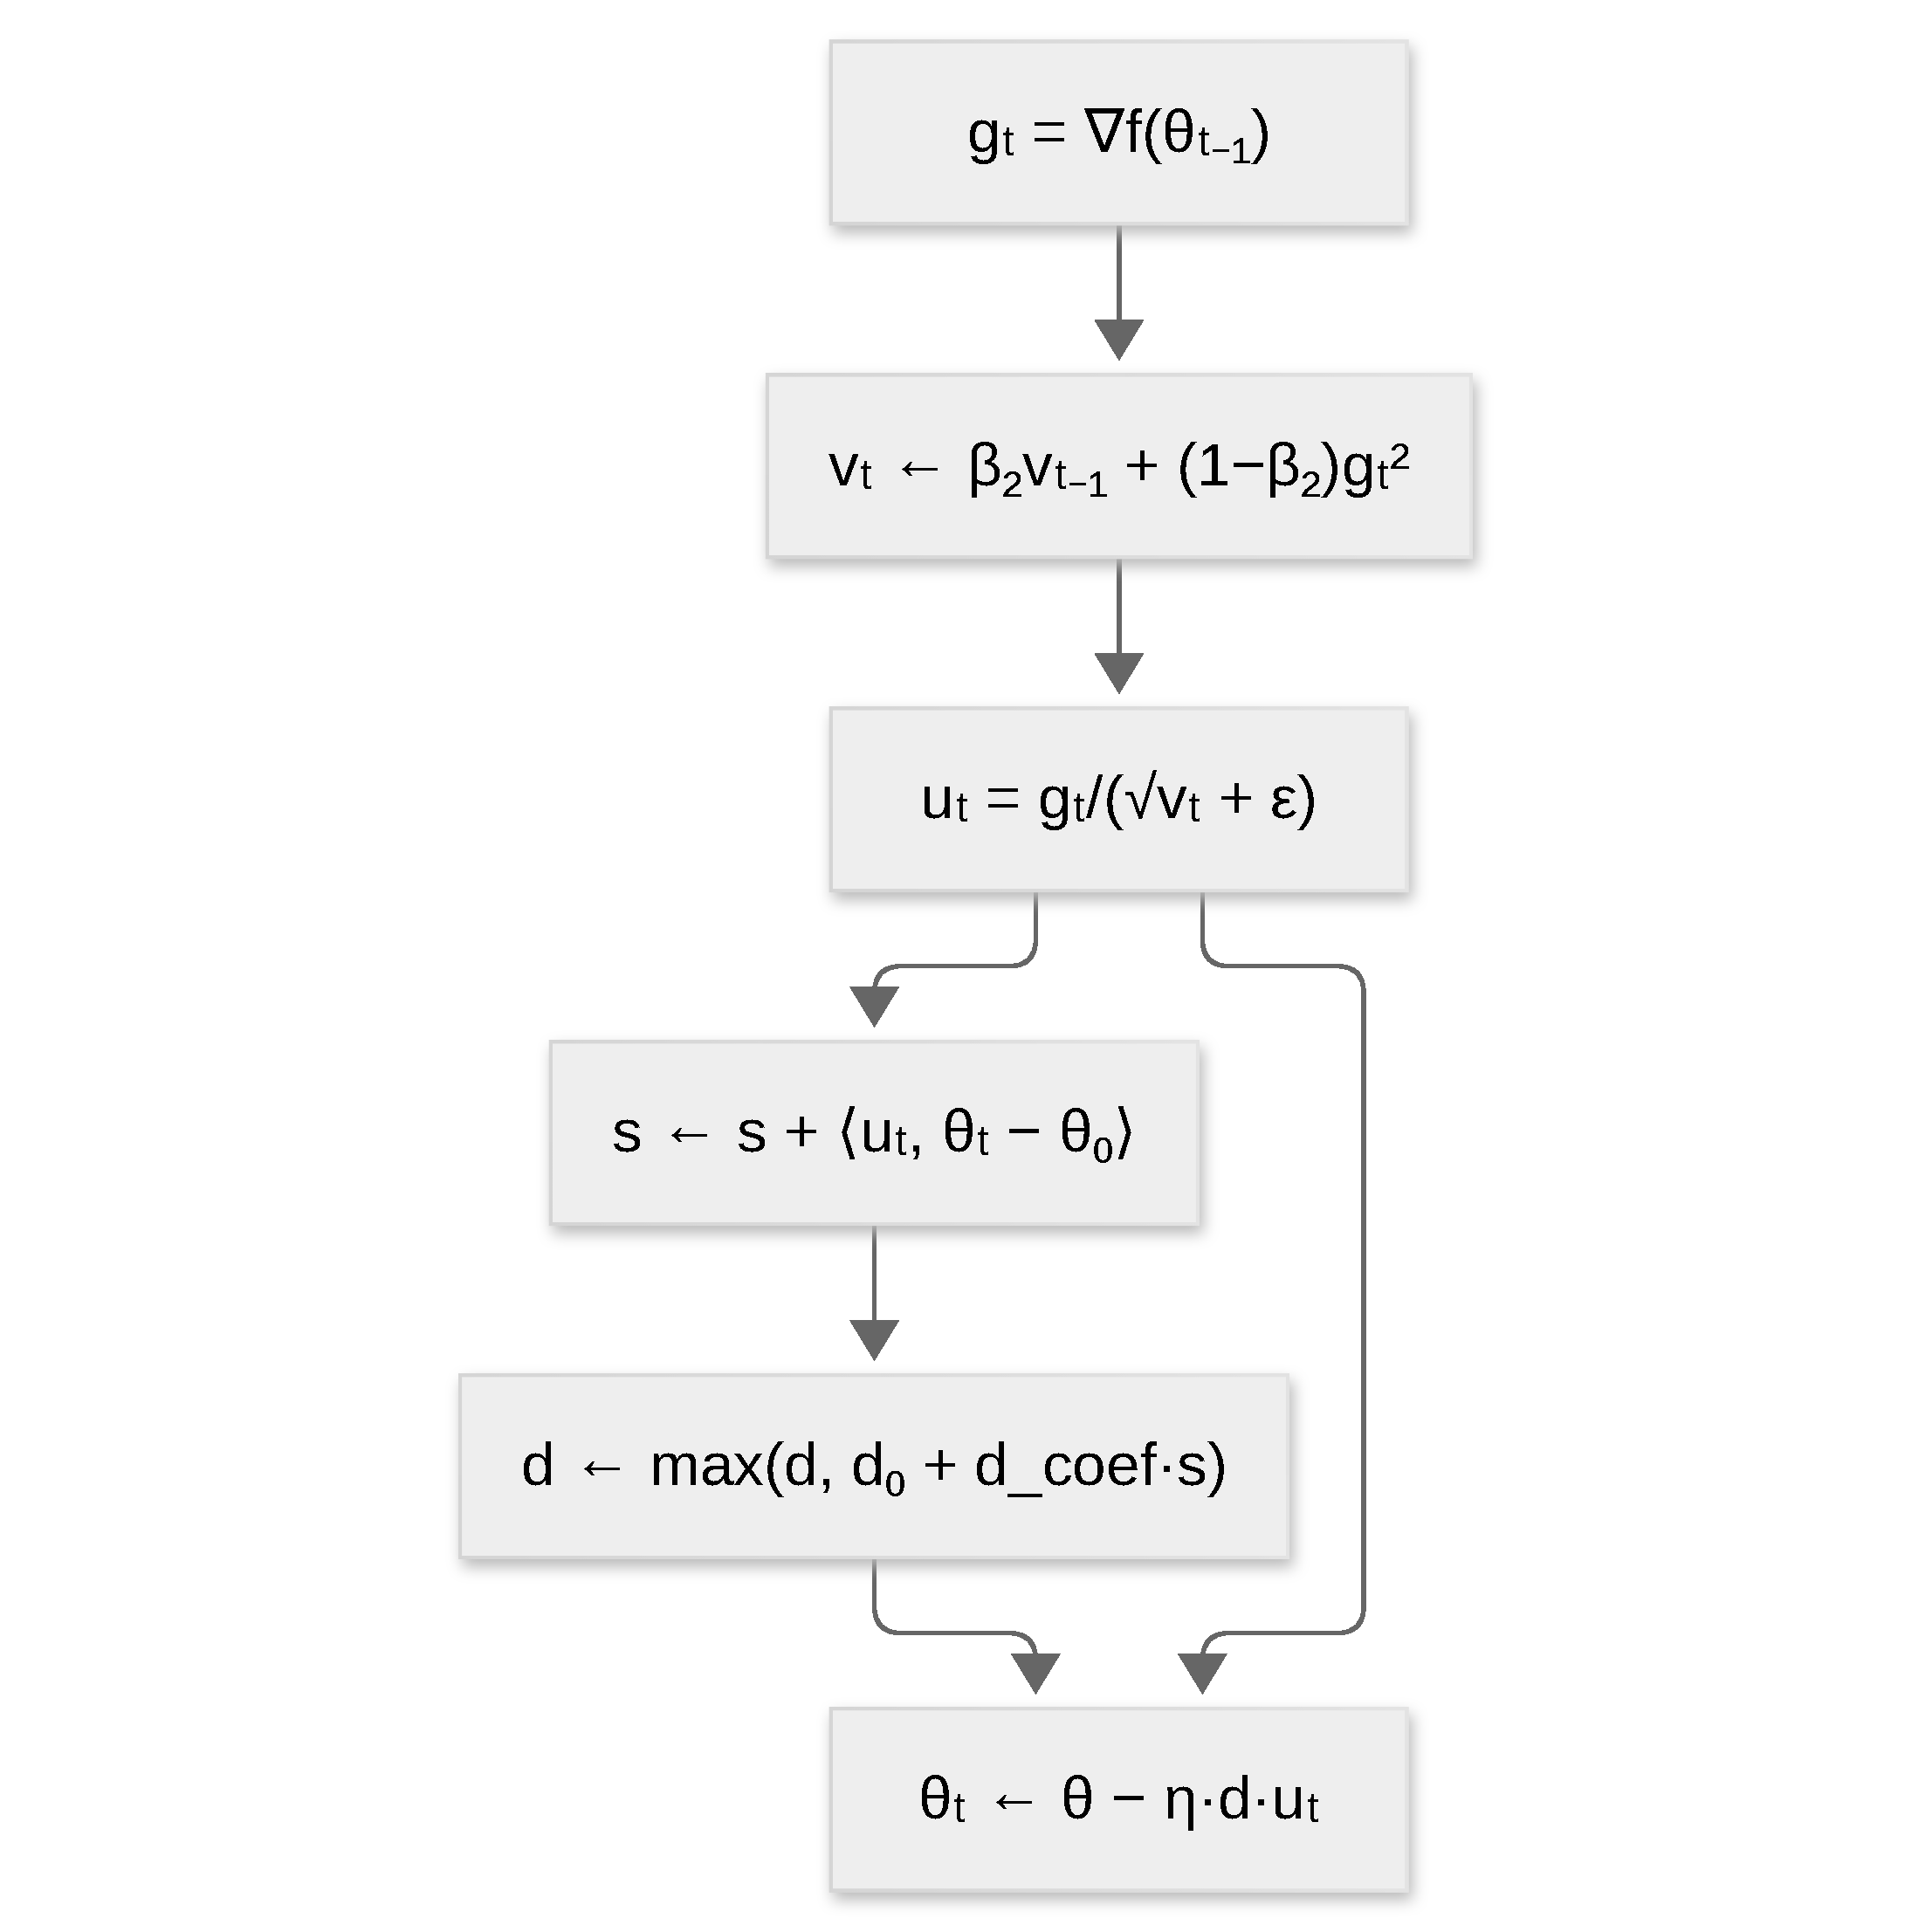
\includegraphics{figures/optimizers/prodigy.pdf}}
\caption{Step flow of Prodigy: a cumulative signed-distance estimate that scales the adaptive step without a learning-rate schedule.}
\label{fig:opt-prodigy}
\end{figure}
Prodigy adapts the effective step scale through a running distance-like statistic, eliminating the need for explicit learning-rate tuning. The algorithm maintains a cumulative distance estimate:
\begin{align}
u_t &= \frac{g_t}{\sqrt{v_t}+\epsilon} \quad\text{(unnormalized adaptive step)} \\
s_t &= s_{t-1} + \langle u_t, \theta_t - \theta_0 \rangle \quad\text{(cumulative signed distance)} \\
d_t &= \max(d_{t-1}, d_0 + d_{\text{coef}} \cdot s_t) \quad\text{(distance estimate with lower bound)} \\
\theta_{t+1} &= \theta_t - \eta \cdot d_t \cdot u_t
\end{align}
where $d_0$ is an initial bound and $d_{\text{coef}}$ controls how aggressively the estimate adapts. The distance estimate $d_t$ captures the combined magnitude of past gradients weighted by actual parameter displacement, implementing an implicit effective learning rate.

\begin{algorithm}[H]
\caption{Prodigy (Approximating the Distance Estimate)}
\label{alg:prodigy}
\begin{algorithmic}[1]
\Require Initial parameters $\theta_0$, learning rate $\eta$, coeff $d_{\text{coef}}$, initial dist $d_0 > 0$
\Ensure Updated parameters $\theta_T$
\State Initialize: $s \gets 0$ (cumulative signed distance), $d \gets d_0$
\For{$t = 1, 2, \ldots, T$}
    \State $g_t \gets \nabla f(\theta_{t-1})$
    \State $v_t \gets \beta_2 v_{t-1} + (1-\beta_2) g_t^2$ \Comment{Second moment}
    \State $u_t \gets g_t / (\sqrt{v_t} + \epsilon)$ \Comment{Unnormalized adaptive}
    \State Update distance: $s \gets s + \langle u_t, \theta_t - \theta_0 \rangle$ \Comment{Signed distance}
    \State $d \gets \max(d, d_0 + d_{\text{coef}} \cdot s)$ \Comment{Lower-bounded distance}
    \State $\theta_t \gets \theta_{t-1} - \eta \cdot d \cdot u_t$ \Comment{Distance-scaled update}
\EndFor
\Return $\theta_T$
\end{algorithmic}
\end{algorithm}

\paragraph{Cons.}
\begin{itemize}[leftmargin=*]
\item Introduces $d_0$ and $d_{\text{coef}}$ hyperparameters for the distance estimate.
\item Adds an inner-product bookkeeping step per iteration.
\end{itemize}

\paragraph{Pros.}
\begin{itemize}[leftmargin=*]
\item Removes explicit learning-rate tuning and scheduling.
\item Robust convergence across problem scales and batch sizes.
\end{itemize}

\subsection{Second-Order, Geometric, and Orthogonality Optimizers}
\paragraph{Shampoo (Matrix Preconditioning via Kronecker Products).}
\begin{figure}[H]
\centering
\fitfigure{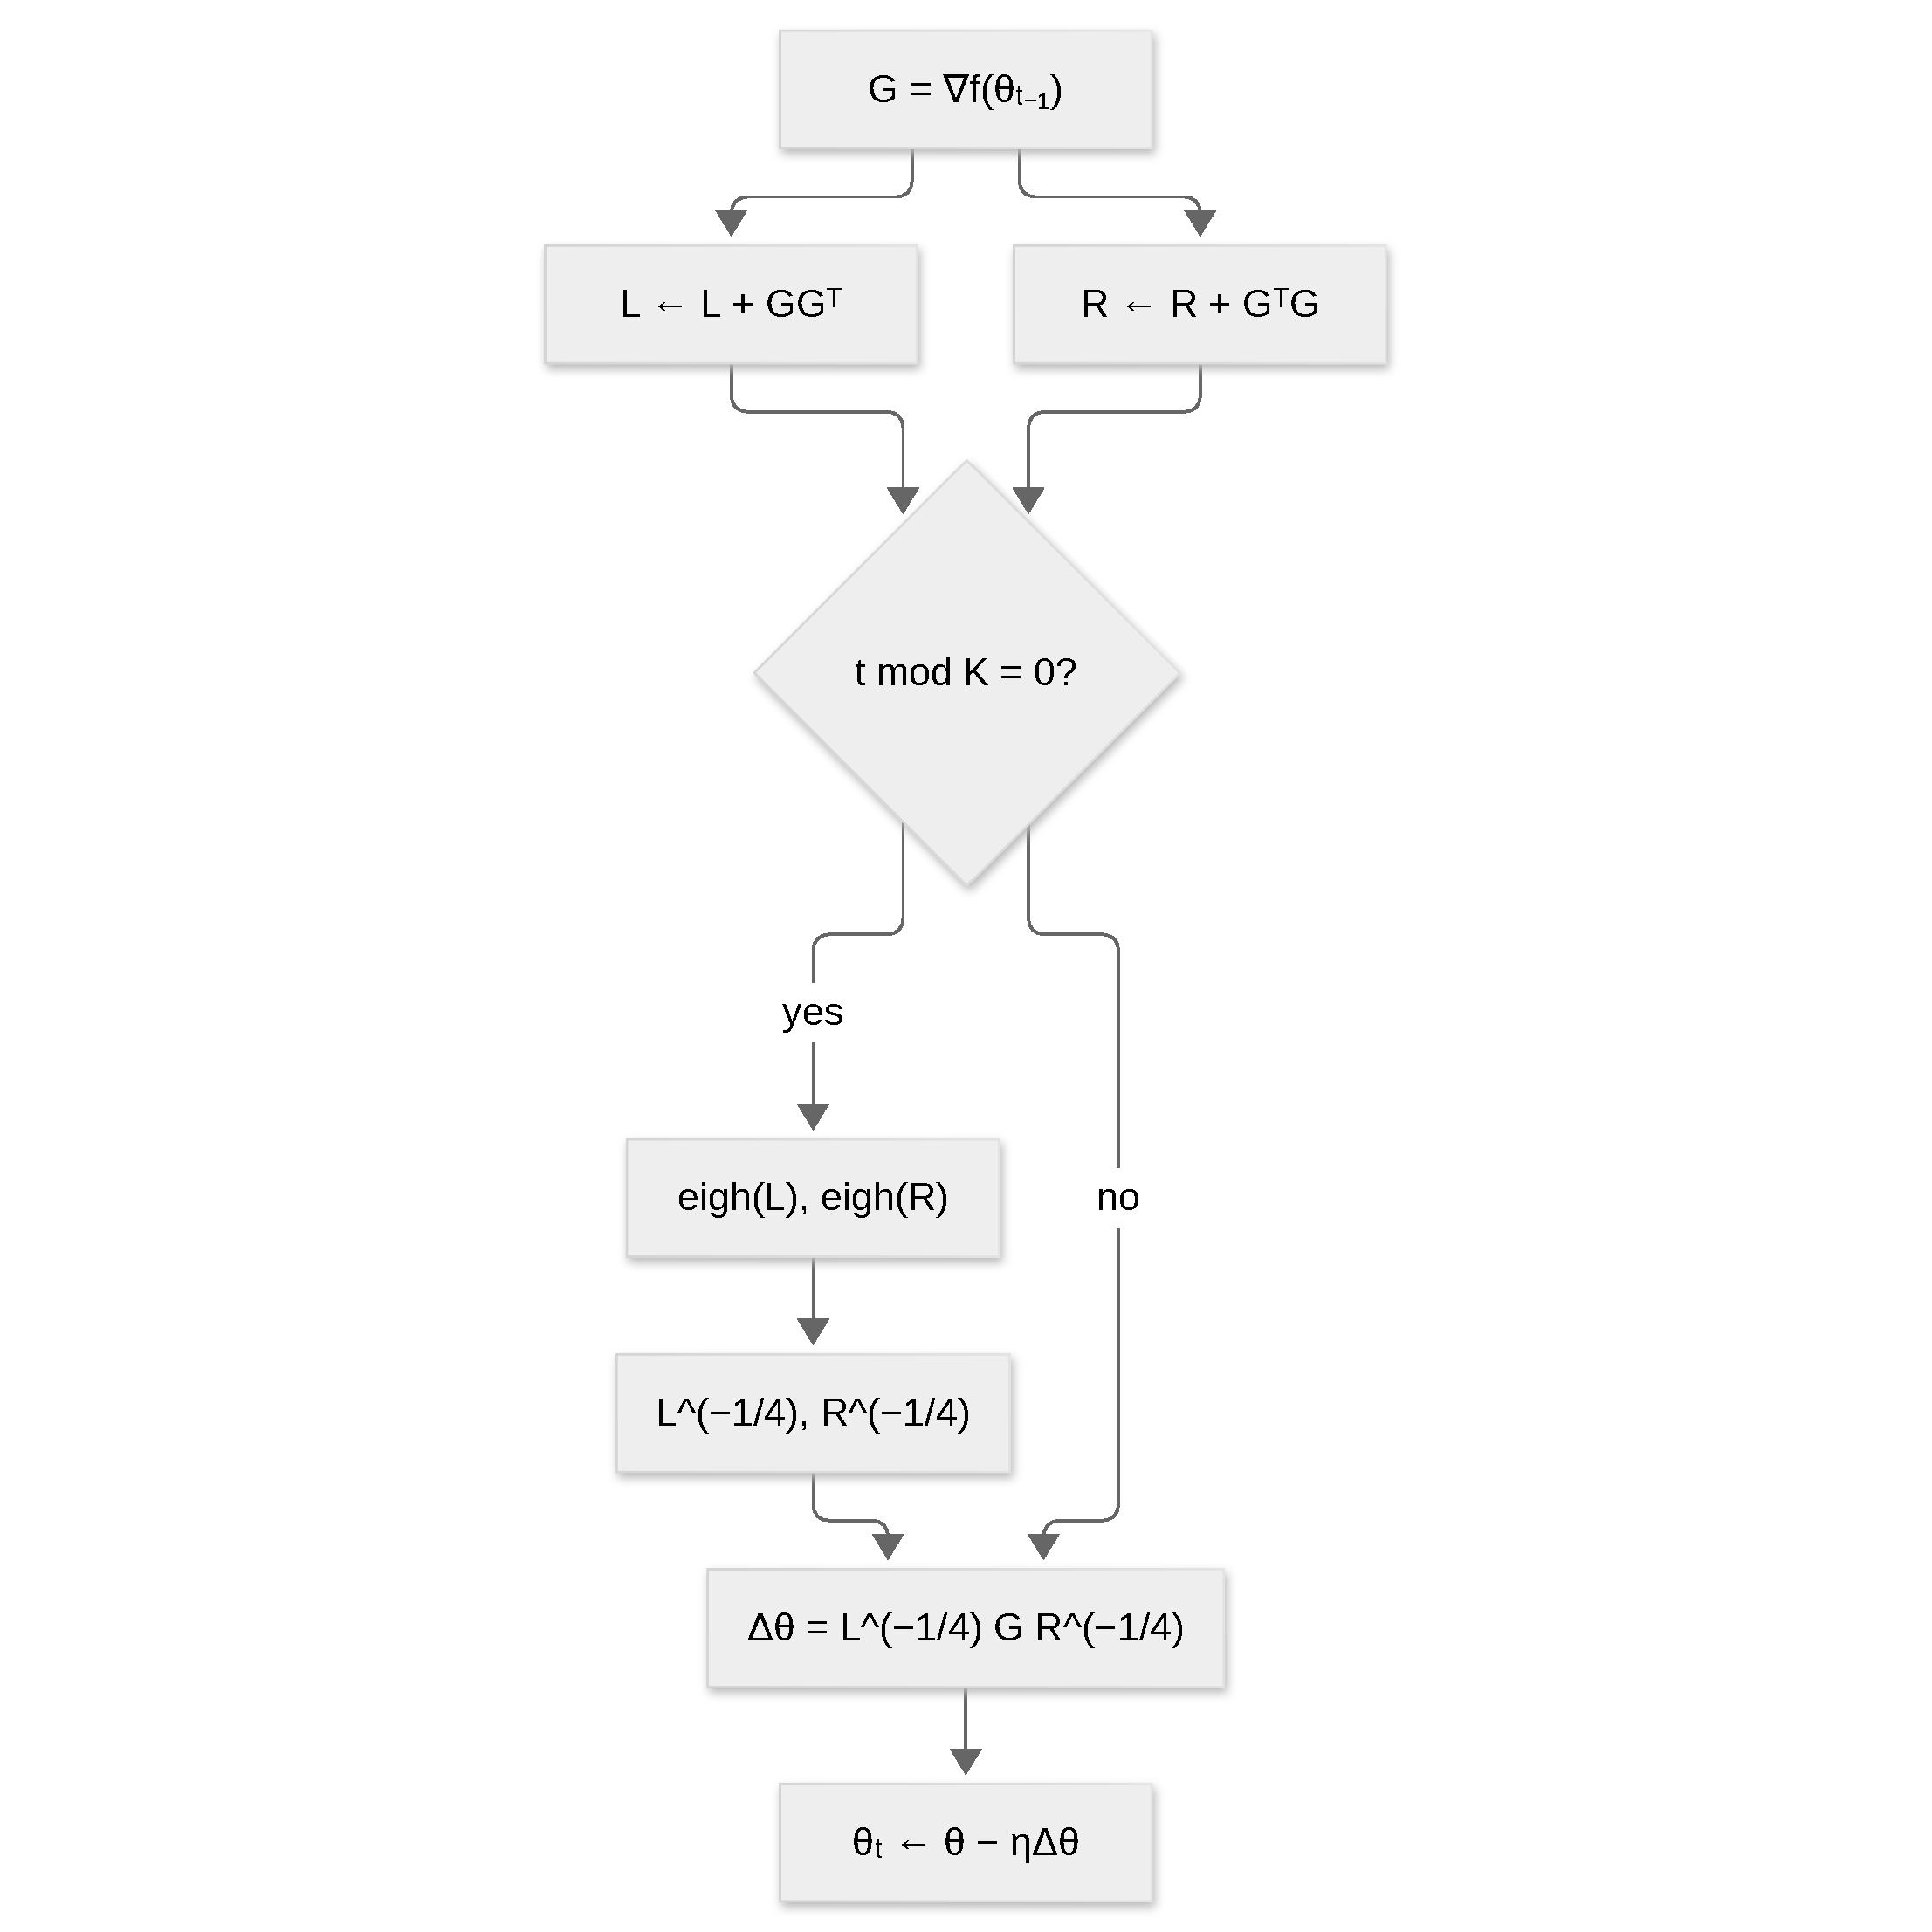
\includegraphics{figures/optimizers/shampoo.pdf}}
\caption{Step flow of Shampoo: Kronecker-factored Gram matrices, periodic eigendecomposition, and fourth-root preconditioning of the gradient.}
\label{fig:opt-shampoo}
\end{figure}
Shampoo is a \textbf{structured second-order method} that computes matrix preconditioners from Kronecker-structured outer-product statistics. For a 2D parameter matrix $W \in \mathbb{R}^{m \times n}$:
\begin{align}
L_t &= L_{t-1} + G_t G_t^\top \quad\text{(left/row Gram matrix, $m \times m$)} \\
R_t &= R_{t-1} + G_t^\top G_t \quad\text{(right/column Gram matrix, $n \times n$)} \\
L_t^{-1/4} &= Q_L (\Lambda_L)^{-1/4} Q_L^\top \quad\text{(via eigendecomposition)} \\
R_t^{-1/4} &= Q_R (\Lambda_R)^{-1/4} Q_R^\top \\
\Delta W_t &= L_t^{-1/4} G_t R_t^{-1/4} \quad\text{(preconditioned gradient)}
\end{align}
Shampoo approximates the full-matrix Adagrad preconditioner $H^{-1/2}$ (where $H$ is the Hessian) using Kronecker-factored structure. Instead of storing a $(mn) \times (mn)$ preconditioner, Shampoo maintains two smaller matrices ($m \times m$ and $n \times n$), capturing cross-parameter correlations within and across groups. Eigendecompositions are performed periodically (e.g., every $K=10$ steps) to amortize cost.

\begin{algorithm}[H]
\caption{Shampoo (Matrix Preconditioning via Kronecker Products)}
\label{alg:shampoo}
\begin{algorithmic}[1]
\Require Initial parameters $\theta_0$, learning rate $\eta$, eigendecomposition interval $K$
\Ensure Updated parameters $\theta_T$
\State Initialize: $L \gets \epsilon I_m$, $R \gets \epsilon I_n$ (left and right Gram matrices)
\For{$t = 1, 2, \ldots, T$}
    \State $G \gets \nabla f(\theta_{t-1})$ \Comment{Gradient}
    \State Update Gram matrices: $L \gets L + G G^\top$, $R \gets R + G^\top G$
    \If{$t \mod K == 0$}
        \State $Q_L, \Lambda_L \gets \text{eigh}(L)$ \Comment{Eigendecomposition of $L$}
        \State $Q_R, \Lambda_R \gets \text{eigh}(R)$ \Comment{Eigendecomposition of $R$}
        \State $L^{-1/4} \gets Q_L (\Lambda_L + \epsilon)^{-1/4} Q_L^\top$
        \State $R^{-1/4} \gets Q_R (\Lambda_R + \epsilon)^{-1/4} Q_R^\top$
    \EndIf
    \State $\Delta \theta \gets L^{-1/4} G R^{-1/4}$ \Comment{Preconditioned gradient}
    \State $\theta_t \gets \theta_{t-1} - \eta \cdot \Delta \theta$
\EndFor
\Return $\theta_T$
\end{algorithmic}
\end{algorithm}

\paragraph{Cons.}
\begin{itemize}[leftmargin=*]
\item Periodic $O(m^3 + n^3)$ eigendecompositions and higher per-step compute.
\item Assumes 2D parameter structure; embeddings and biases need separate handling.
\end{itemize}

\paragraph{Pros.}
\begin{itemize}[leftmargin=*]
\item Kronecker-factored second-order preconditioning without a dense $(mn) \times (mn)$ matrix.
\item Proven effective at production scale and well suited to high-rank transformer matrices, with improved conditioning and accelerated convergence.
\end{itemize}

\paragraph{SOAP (Shampoo with Adam in eigenbasis).}
\begin{figure}[H]
\centering
\fitfigure{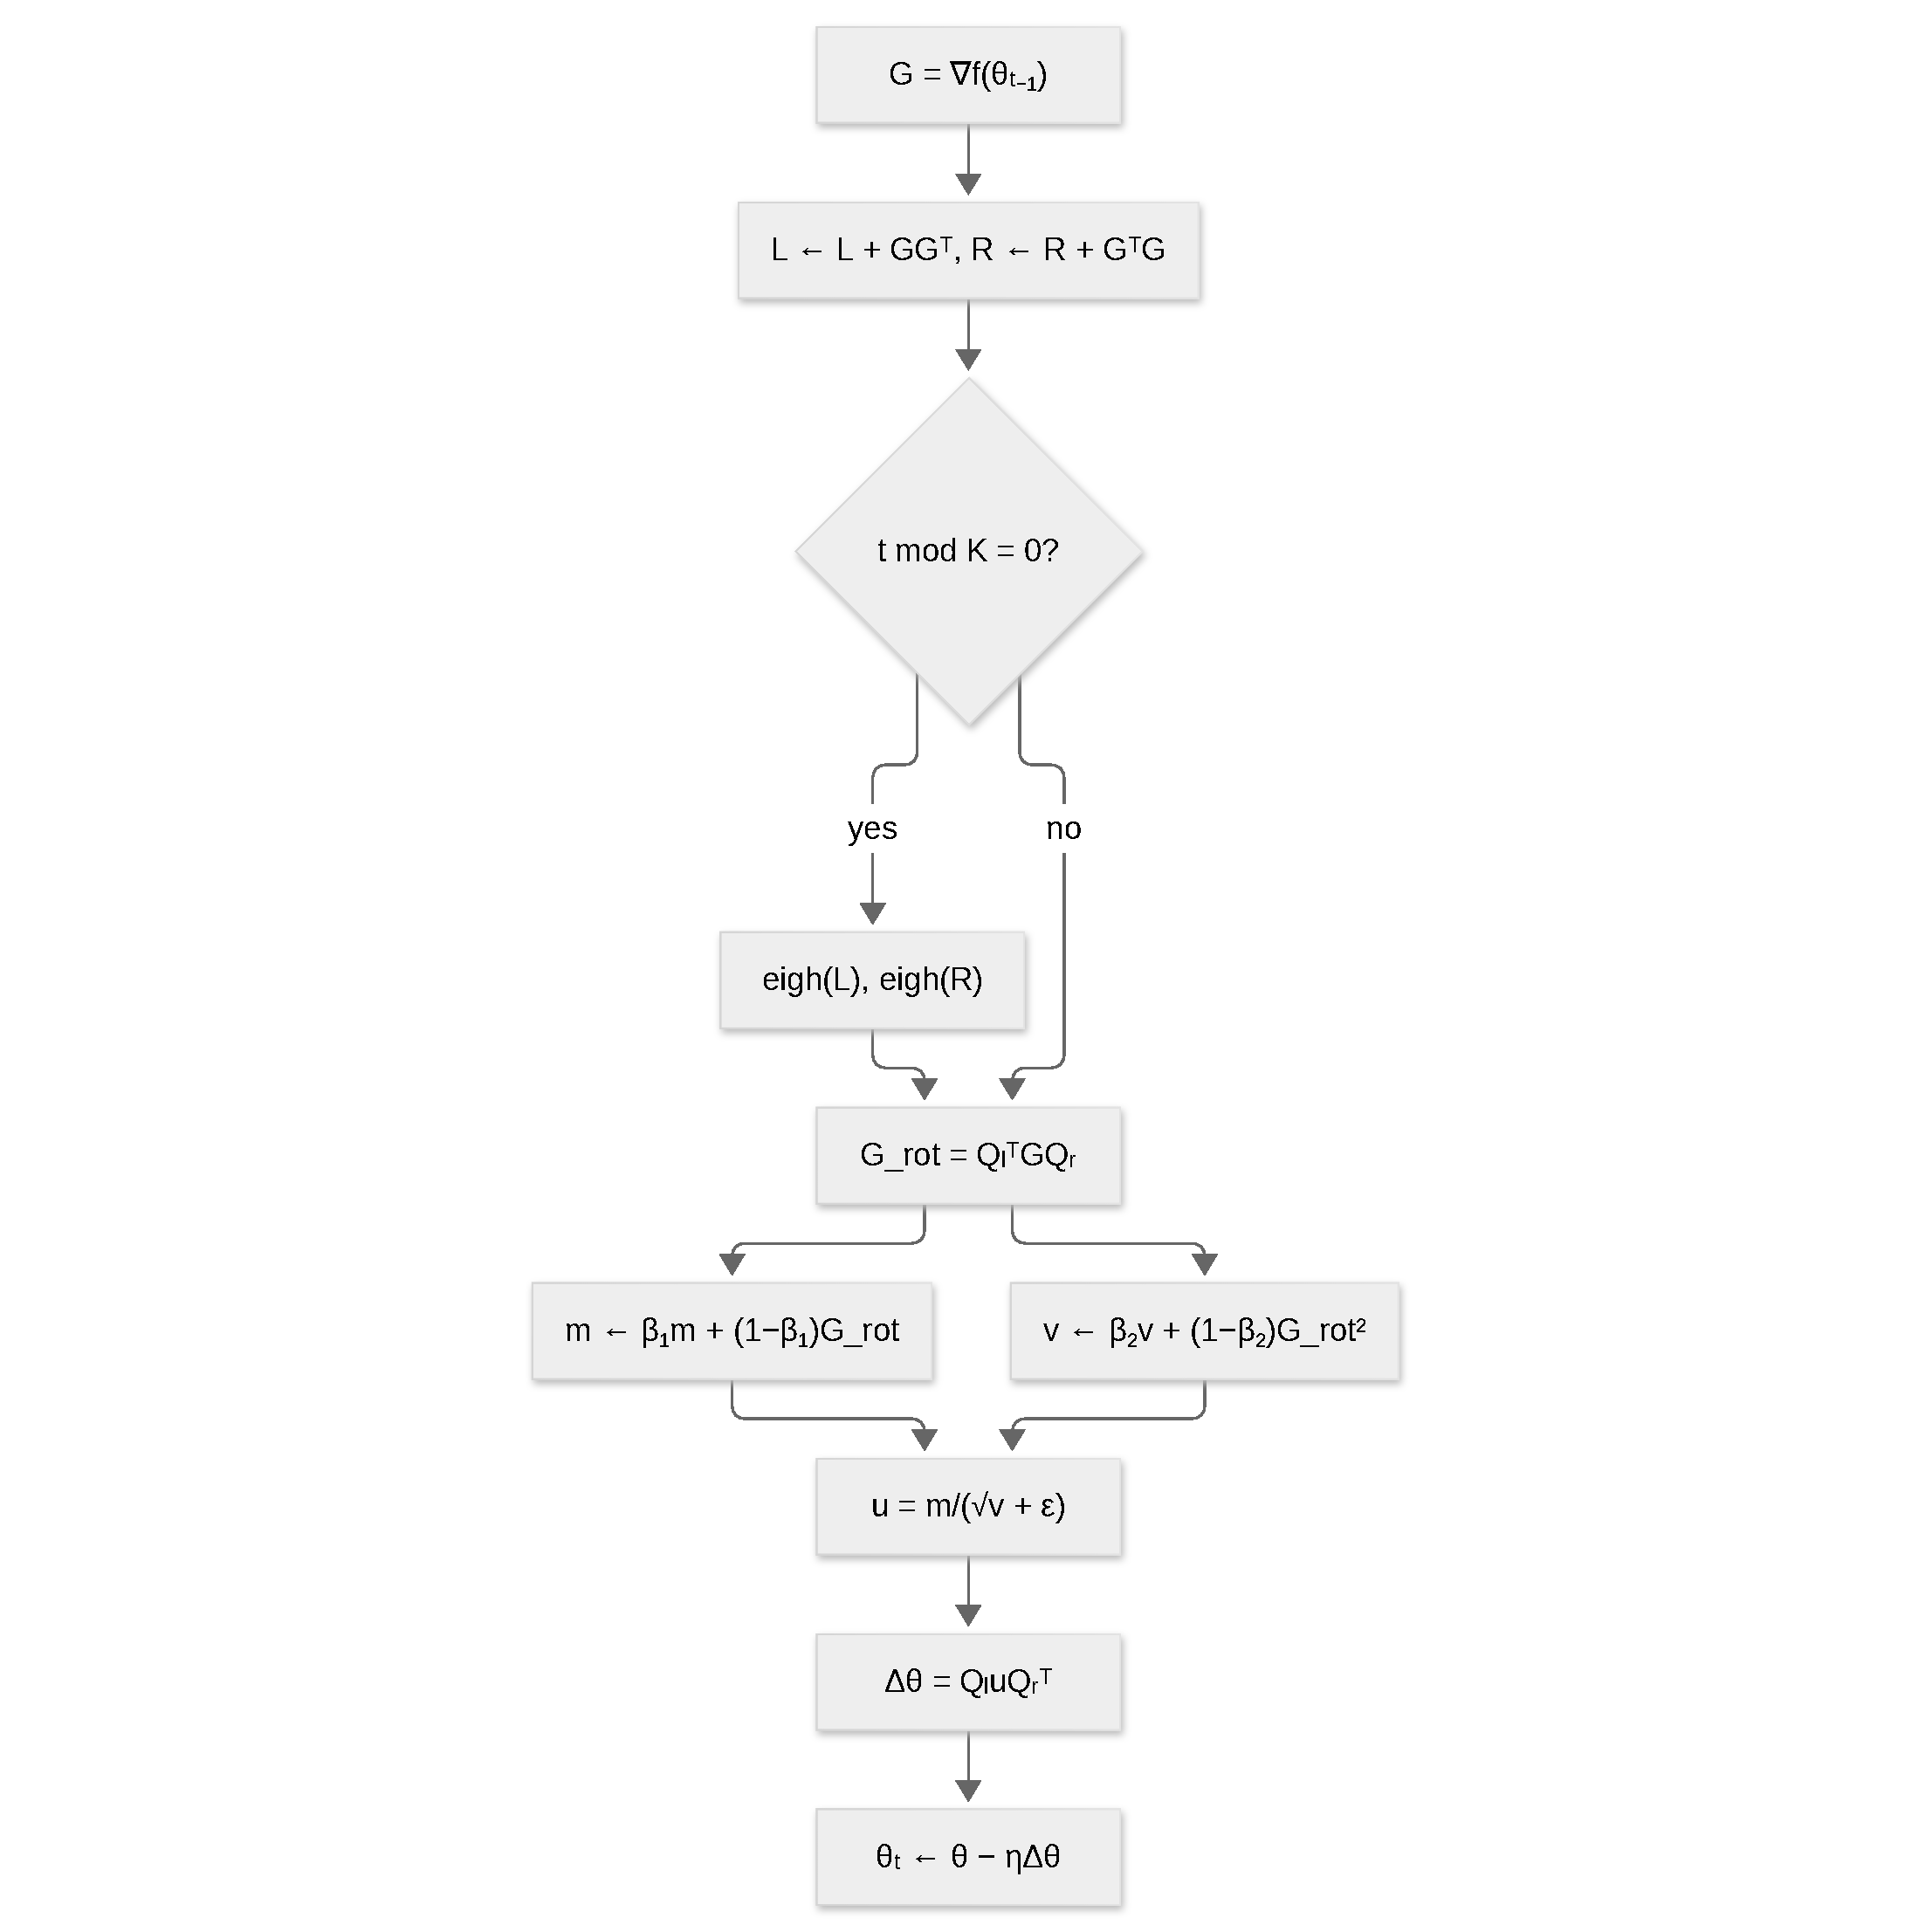
\includegraphics{figures/optimizers/soap.pdf}}
\caption{Step flow of SOAP: Adam moments tracked in the Shampoo eigenbasis and rotated back to parameter space.}
\label{fig:opt-soap}
\end{figure}
SOAP is a simplified variant of Shampoo that decouples preconditioning from momentum tracking. Instead of complex matrix algebra on preconditioned gradients, SOAP runs standard Adam in the eigenbasis of Shampoo's preconditioners:
\begin{align}
L_t &= L_{t-1} + G_t G_t^\top, \quad R_t = R_{t-1} + G_t^\top G_t \quad\text{(Gram accumulation)} \\
Q_L, \Lambda_L &= \text{eigh}(L_t), \quad Q_R, \Lambda_R = \text{eigh}(R_t) \quad\text{(periodic eigendecomposition)} \\
G_t^{\text{rot}} &= Q_L^\top G_t Q_R \quad\text{(rotate gradient into eigenbasis)} \\
m_t^{\text{rot}} &= \beta_1 m_{t-1}^{\text{rot}} + (1-\beta_1) G_t^{\text{rot}} \\
v_t^{\text{rot}} &= \beta_2 v_{t-1}^{\text{rot}} + (1-\beta_2)(G_t^{\text{rot}})^2 \quad\text{(Adam in rotated space)} \\
U_t^{\text{rot}} &= \frac{m_t^{\text{rot}}}{\sqrt{v_t^{\text{rot}}}+\epsilon}, \quad U_t = Q_L U_t^{\text{rot}} Q_R^\top \quad\text{(rotate back)}
\end{align}
The key insight: all momentum tracking occurs in the well-conditioned eigenbasis, simplifying numerical stability and theoretical analysis.

\begin{algorithm}[H]
\caption{SOAP (Shampoo with Adam in Eigenbasis)}
\label{alg:soap}
\begin{algorithmic}[1]
\Require Initial parameters $\theta_0$, learning rate $\eta$, $\beta_1, \beta_2$, eigendecomposition interval $K$
\Ensure Updated parameters $\theta_T$
\State Initialize: $L \gets \epsilon I_m$, $R \gets \epsilon I_n$, $m \gets 0$, $v \gets 0$
\For{$t = 1, 2, \ldots, T$}
    \State $G \gets \nabla f(\theta_{t-1})$ \Comment{Gradient}
    \State Update Gram: $L \gets L + G G^\top$, $R \gets R + G^\top G$
    \If{$t \mod K == 0$}
        \State $Q_L, \Lambda_L \gets \text{eigh}(L)$, $Q_R, \Lambda_R \gets \text{eigh}(R)$
    \EndIf
    \State $G^{\text{rot}} \gets Q_L^\top G Q_R$ \Comment{Rotate gradient into eigenbasis}
    \State $m \gets \beta_1 m + (1-\beta_1) G^{\text{rot}}$ \Comment{Exponential moving average (bias-correct outside)}
    \State $v \gets \beta_2 v + (1-\beta_2) (G^{\text{rot}})^2$ \Comment{Second moment (bias-correct outside)}
    \State $u \gets m / (\sqrt{v} + \epsilon)$ \Comment{Adaptive step in eigenbasis}
    \State $\Delta \theta \gets Q_L u Q_R^\top$ \Comment{Rotate back to parameter space}
    \State $\theta_t \gets \theta_{t-1} - \eta \cdot \Delta \theta$
\EndFor
\Return $\theta_T$
\end{algorithmic}
\end{algorithm}

\paragraph{Cons.}
\begin{itemize}[leftmargin=*]
\item Inherits Shampoo's periodic eigendecomposition cost.
\item Rotation and inverse rotation add matrix multiplications per step.
\end{itemize}

\paragraph{Pros.}
\begin{itemize}[leftmargin=*]
\item Combines Shampoo's explicit curvature structure with Adam's proven momentum mechanics.
\item Often cleaner and more stable than full Shampoo, with eigendecompositions amortized every $K$ steps.
\end{itemize}

\paragraph{Lion (EvoLved Sign Momentum).}
\begin{figure}[H]
\centering
\fitfigure{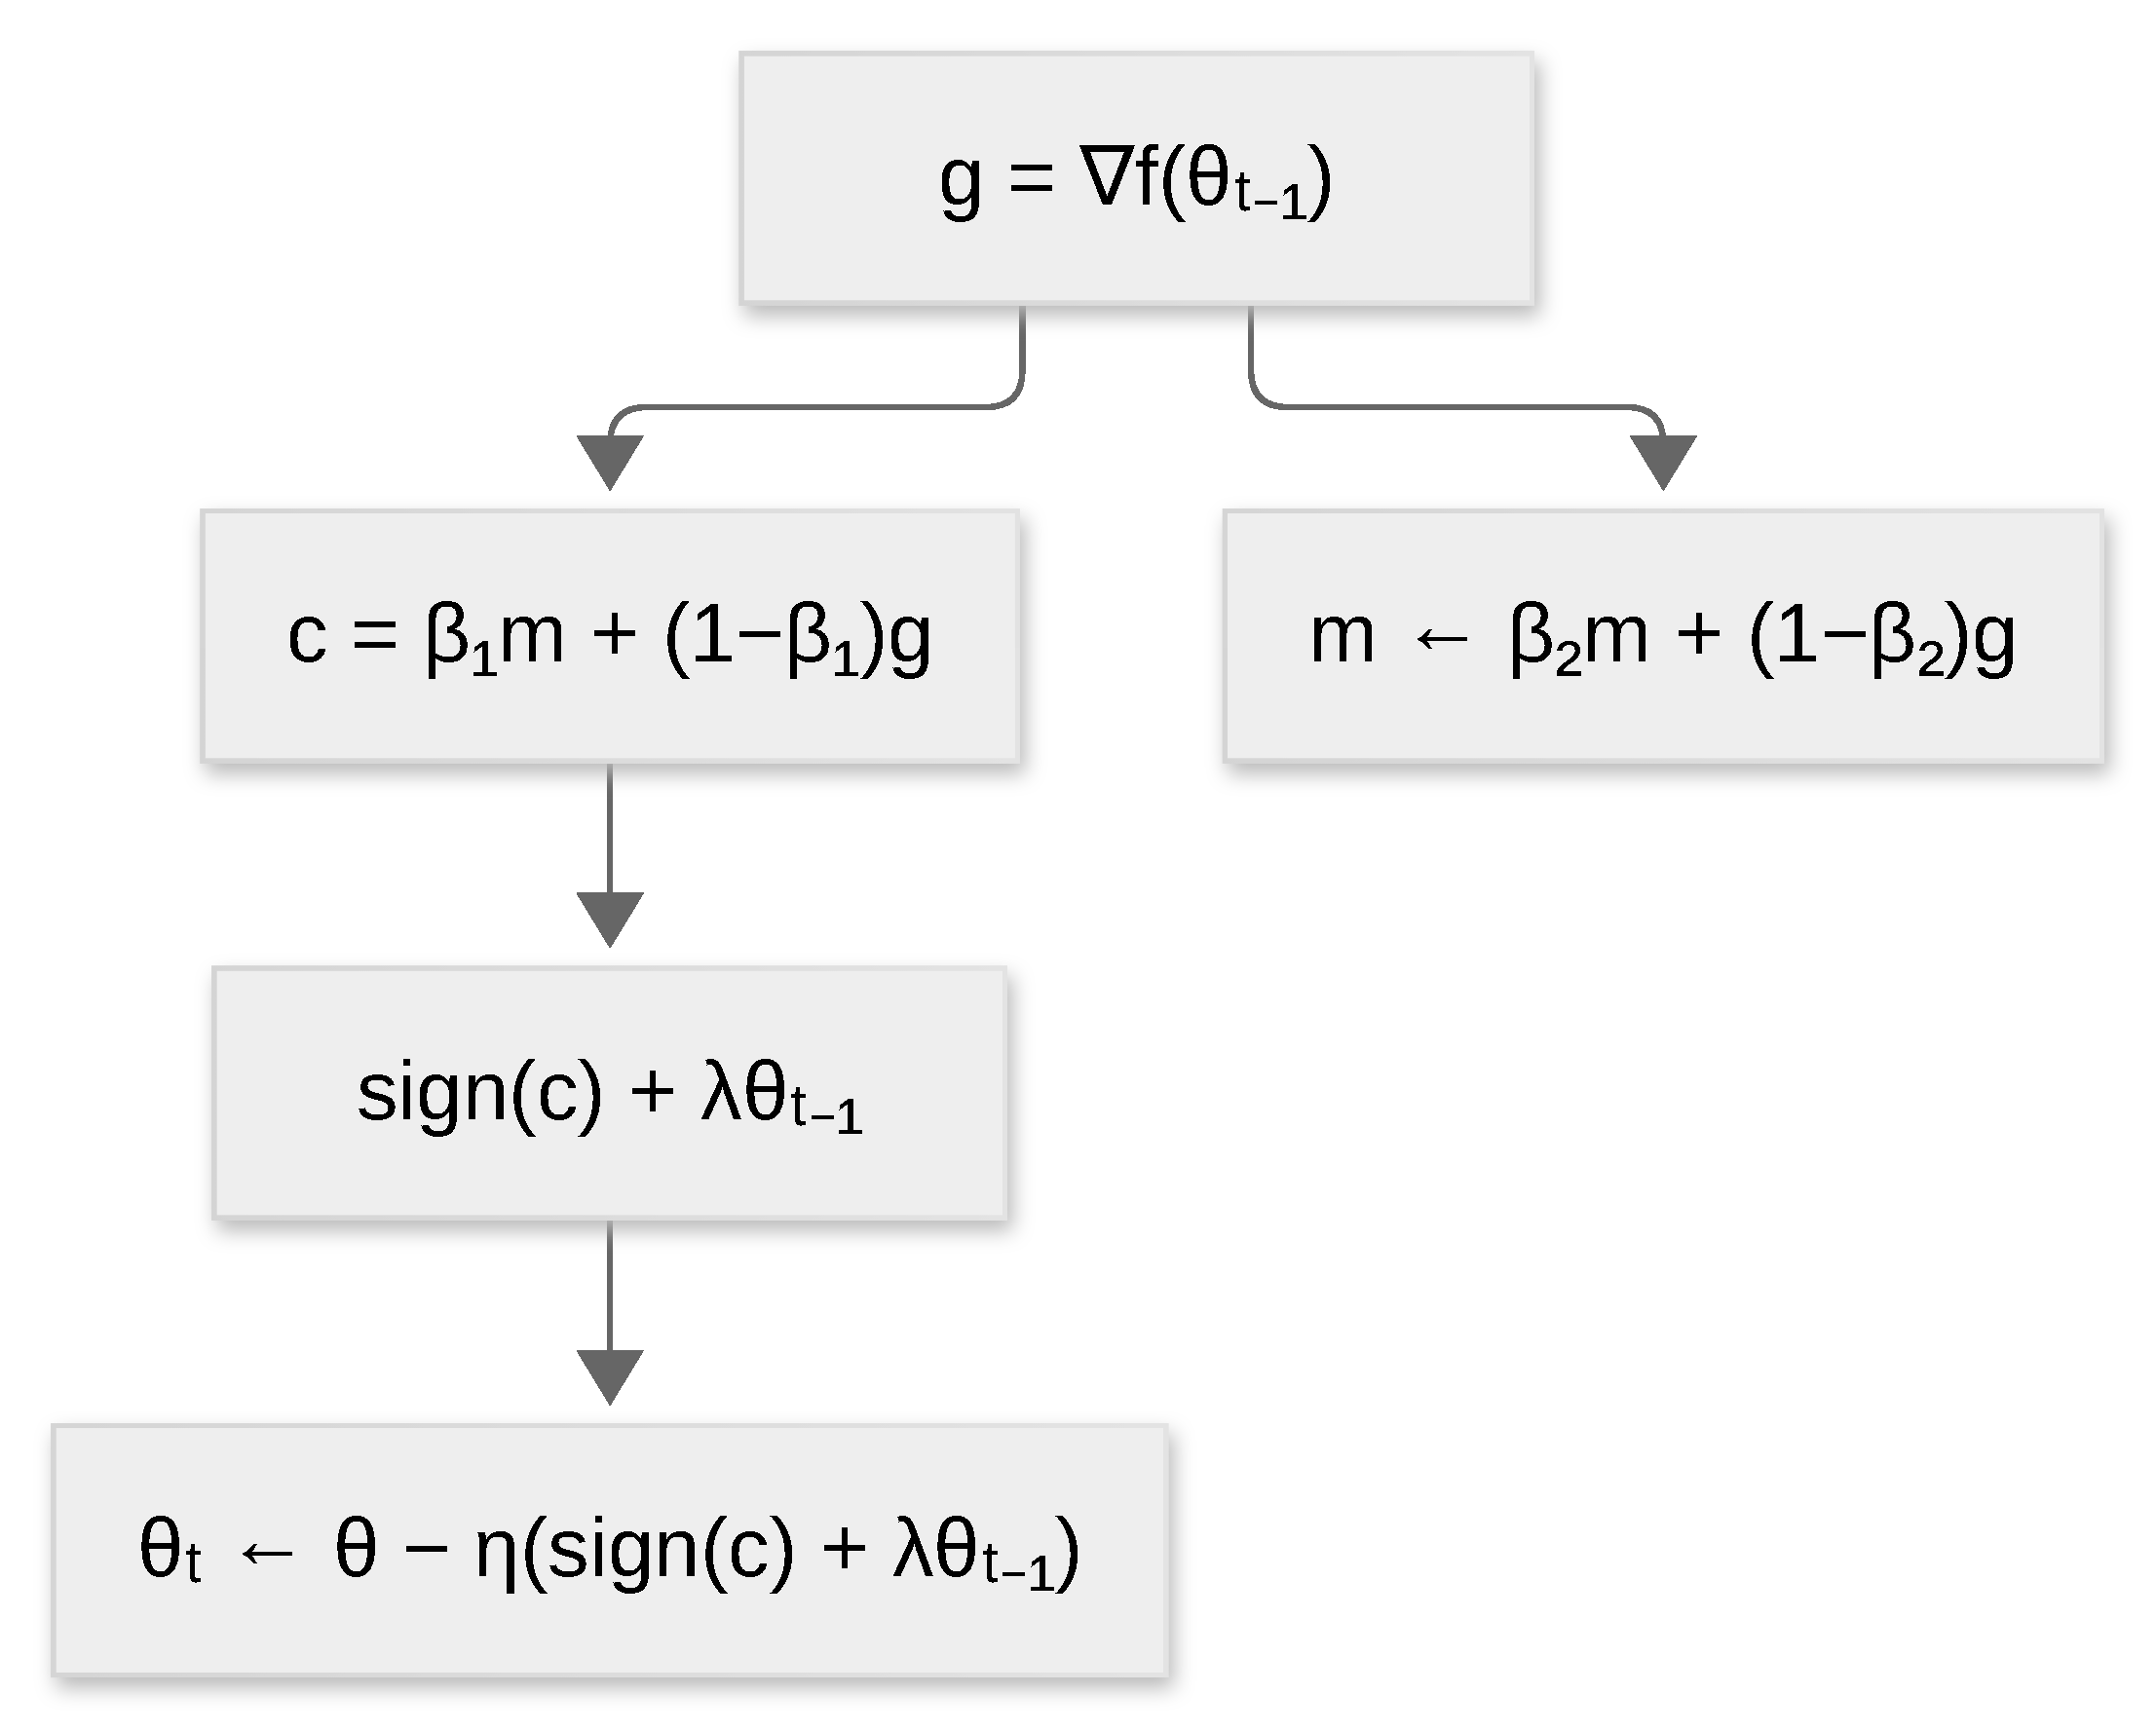
\includegraphics{figures/optimizers/lion.pdf}}
\caption{Step flow of Lion: sign-of-momentum update with decoupled momentum accumulation and weight decay.}
\label{fig:opt-lion}
\end{figure}
Lion achieves \textbf{minimal memory overhead} by using sign-based updates instead of full adaptive scaling:
\begin{align}
c_t &= \beta_1 m_t + (1-\beta_1) g_t \quad\text{(momentum input)} \\
\theta_{t+1} &= \theta_t - \eta \left(\text{sign}(c_t) + \lambda\theta_t\right) \quad\text{(sign operator update)} \\
m_{t+1} &= \beta_2 m_t + (1-\beta_2) g_t \quad\text{(momentum accumulation)}
\end{align}
All element-wise scaling operations are replaced with \texttt{sign()}, which outputs $\{-1, 0, +1\}$. This dramatically reduces memory compared to Adam-like methods: Lion stores only the momentum buffer, no second moment variance.

\begin{algorithm}[H]
\caption{Lion (EvoLved Sign Momentum)}
\label{alg:lion}
\begin{algorithmic}[1]
\Require Initial parameters $\theta_0$, learning rate $\eta$, $\beta_1, \beta_2$, weight decay $\lambda$
\Ensure Updated parameters $\theta_T$
\State Initialize: $m \gets 0$ (momentum buffer)
\For{$t = 1, 2, \ldots, T$}
    \State $g \gets \nabla f(\theta_{t-1})$ \Comment{Gradient}
    \State $c \gets \beta_1 m + (1-\beta_1) g$ \Comment{Momentum input}
    \State $\theta_t \gets \theta_{t-1} - \eta (\text{sign}(c) + \lambda \theta_{t-1})$ \Comment{Sign-based update with weight decay}
    \State $m \gets \beta_2 m + (1-\beta_2) g$ \Comment{Momentum accumulation (decoupled)}
\EndFor
\Return $\theta_T$
\end{algorithmic}
\end{algorithm}

\paragraph{Cons.}
\begin{itemize}[leftmargin=*]
\item Sign-based updates sacrifice the element-wise learning-rate adaptation that makes Adam effective.
\item Can be less robust than Adam-family methods on tasks that need adaptive scaling.
\end{itemize}

\paragraph{Pros.}
\begin{itemize}[leftmargin=*]
\item Stores only the momentum buffer, with no second moment variance.
\item High-throughput, low-memory option for large-batch regimes where activation memory dominates.
\end{itemize}

\paragraph{Sophia (Second-Order Hessian Information with Optimized Approximation).}
\begin{figure}[H]
\centering
\fitfigure{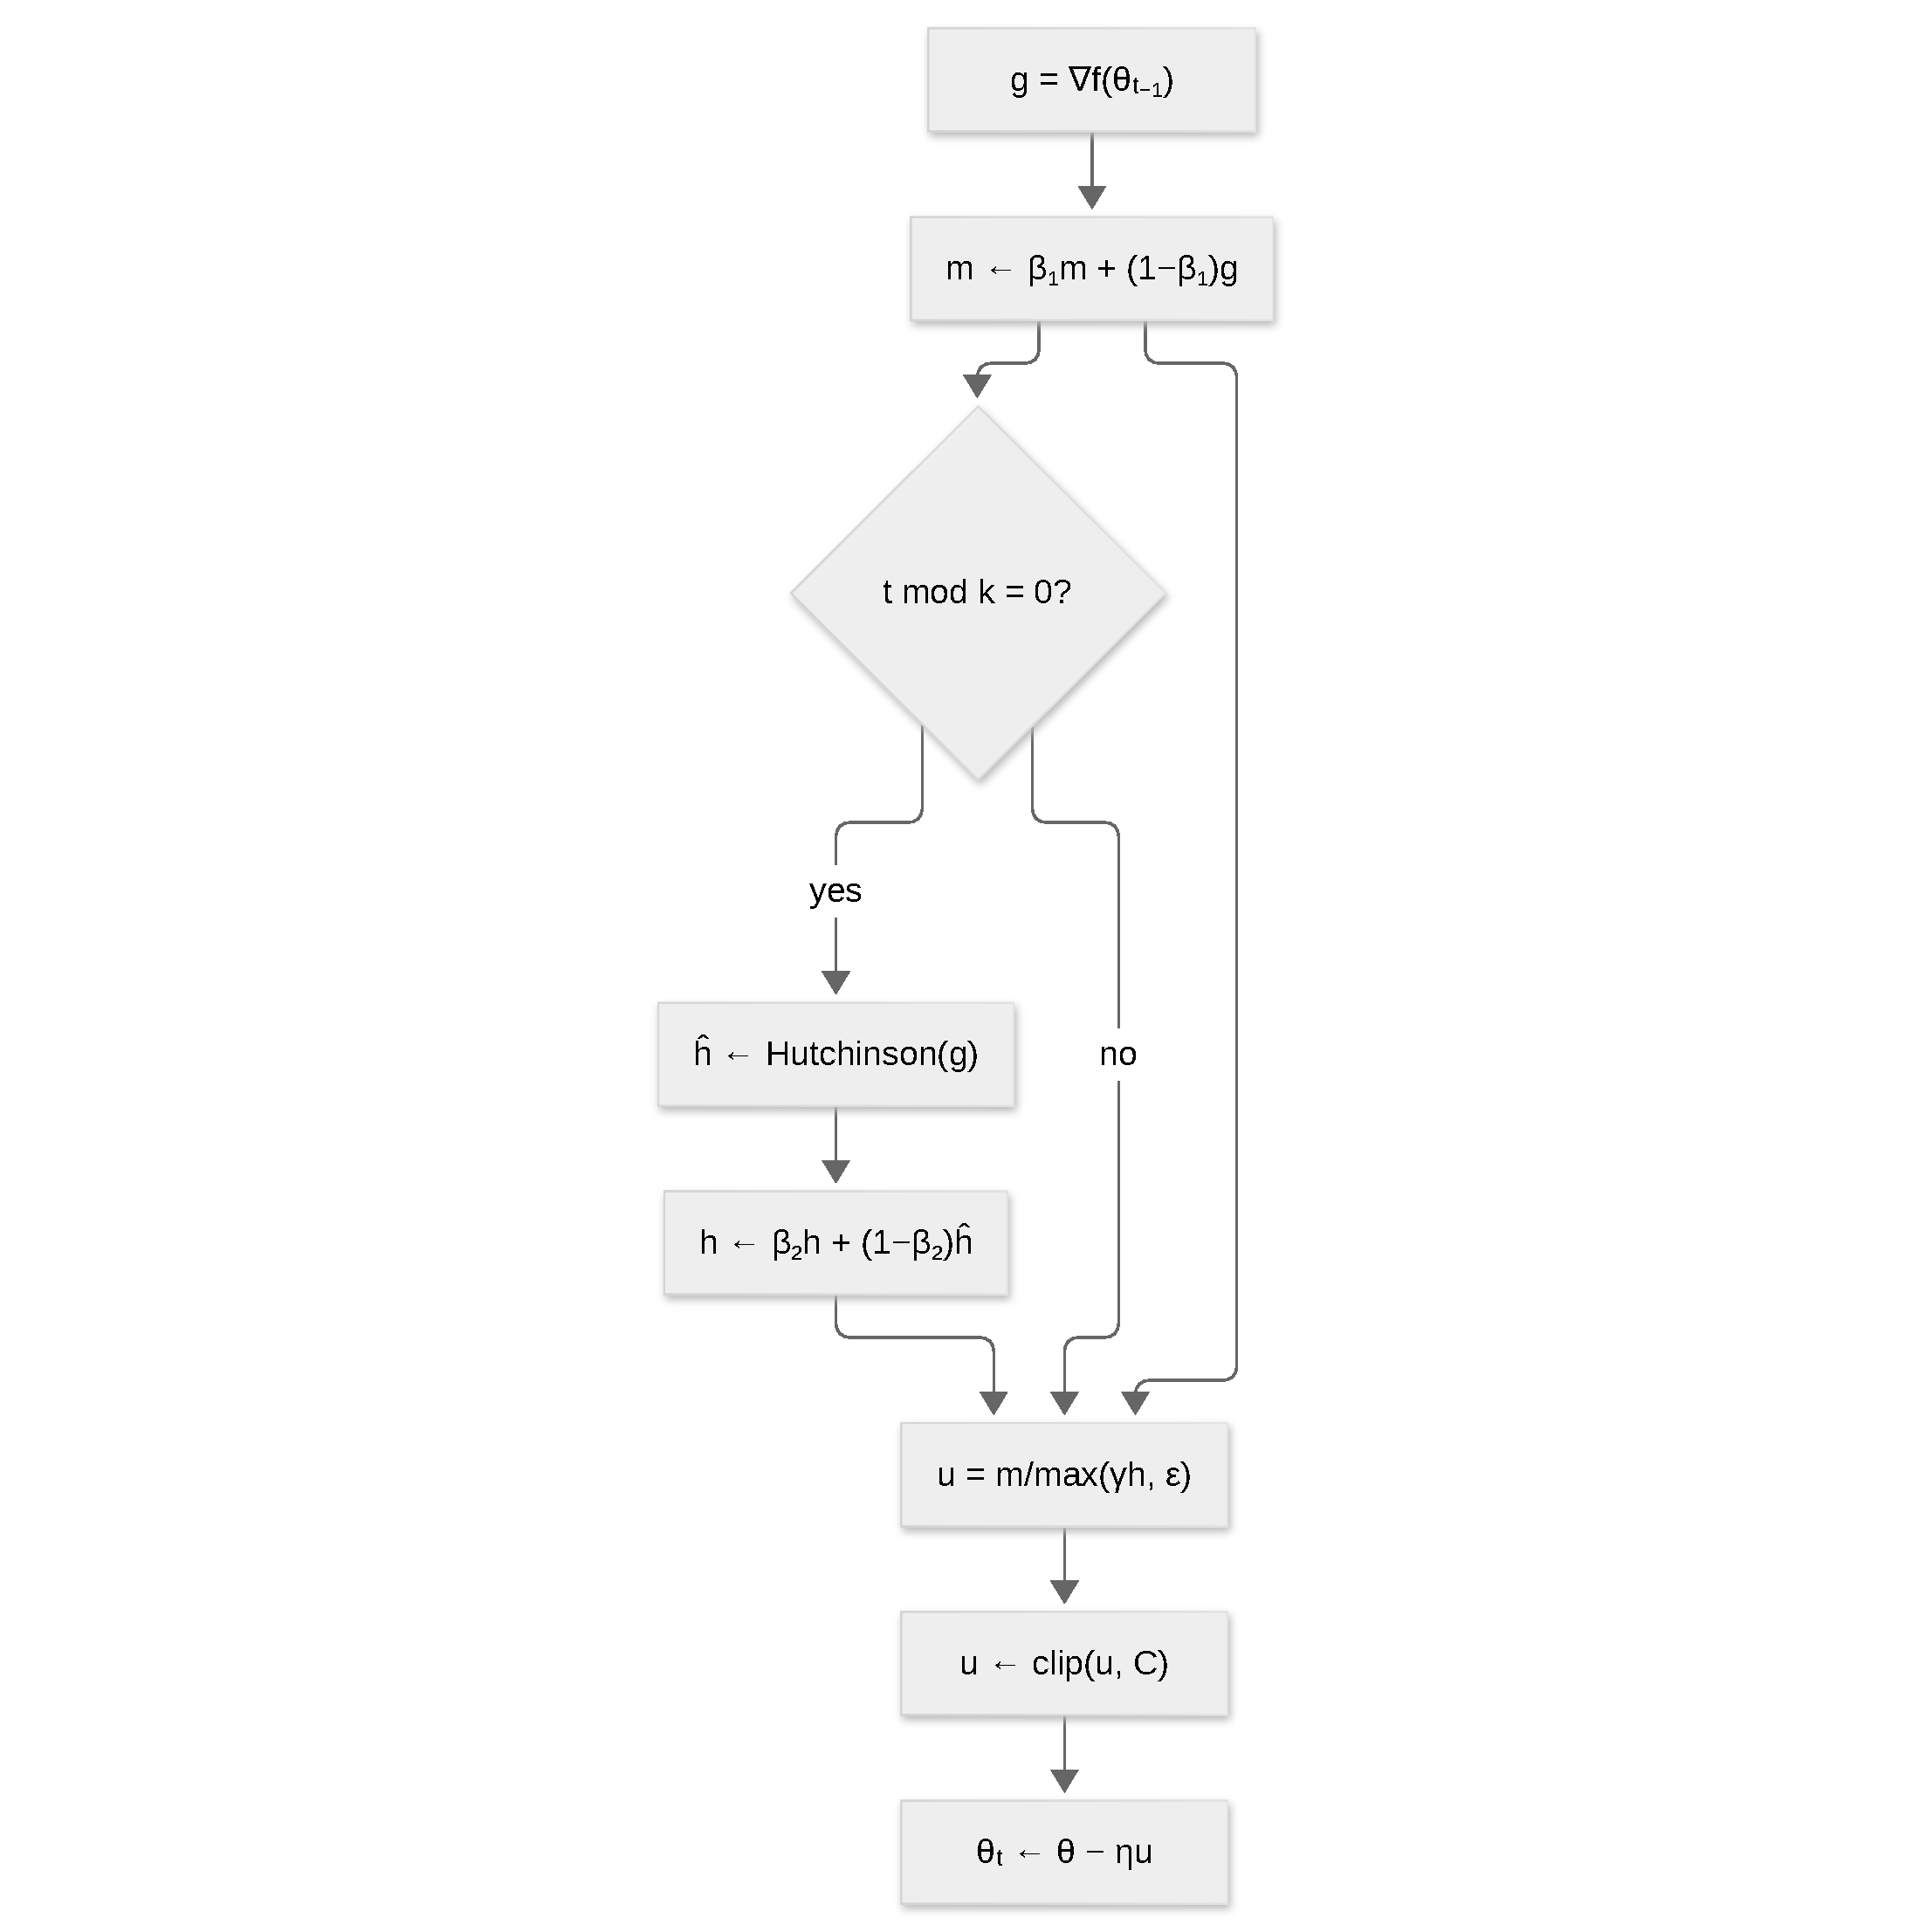
\includegraphics{figures/optimizers/sophia.pdf}}
\caption{Step flow of Sophia: diagonal Hutchinson Hessian estimate with clipped, curvature-aware element-wise steps.}
\label{fig:opt-sophia}
\end{figure}
Sophia uses \textbf{diagonal Hessian estimates} for curvature-aware scaling without the memory and compute cost of dense second-order methods.
\begin{align}
m_t &= \beta_1 m_{t-1} + (1-\beta_1) g_t \quad\text{(first moment)} \\
h_t &= \beta_2 h_{t-(k-1)} + (1-\beta_2) \hat{h}_t \quad\text{(diagonal Hessian, updated every $k$ steps)} \\
\text{clip}(x, C) &= \min(\max(x, -C), C) \quad\text{(element-wise clipping)} \\
\theta_{t+1} &= \theta_t - \eta \cdot \text{clip}\left(\frac{m_t}{\max(\gamma h_t, \epsilon)}, 1\right)
\end{align}
where $\hat{h}_t$ is a diagonal estimate (e.g., Hutchinson-trace estimator) and $\gamma$ is a scaling factor. The diagonal Hessian $h_t$ captures local curvature, allowing the optimizer to take smaller steps in sharp directions and larger steps in flat directions. The clipping operation $\text{clip}(\cdot, 1)$ prevents adaptive steps from exploding.

\begin{algorithm}[H]
\caption{Sophia (Diagonal Hessian with Clipped Updates)}
\label{alg:sophia}
\begin{algorithmic}[1]
\Require Initial parameters $\theta_0$, learning rate $\eta$, $\beta_1, \beta_2$, Hessian update freq $k$, clip threshold $C$
\Ensure Updated parameters $\theta_T$
\State Initialize: $m \gets 0$, $h \gets \epsilon$ (diagonal Hessian estimate)
\For{$t = 1, 2, \ldots, T$}
    \State $g \gets \nabla f(\theta_{t-1})$
    \State $m \gets \beta_1 m + (1-\beta_1) g$ \Comment{First moment (bias-correct outside)}
    \If{$t \mod k == 0$}
        \State $\hat{h} \gets \text{HutchinsonEstimate}(g)$ \Comment{Diagonal Hessian via Hutchinson}
        \State $h \gets \beta_2 h + (1-\beta_2) \hat{h}$ \Comment{Update Hessian estimate}
    \EndIf
    \State $u \gets \frac{m}{\max(\gamma h, \epsilon)}$ \Comment{Adaptive step (element-wise)}
    \State $u \gets \text{clip}(u, C)$ \Comment{Element-wise clipping to $[-C, C]$}
    \State $\theta_t \gets \theta_{t-1} - \eta \cdot u$
\EndFor
\Return $\theta_T$
\end{algorithmic}
\end{algorithm}

\paragraph{Cons.}
\begin{itemize}[leftmargin=*]
\item Hutchinson estimates add periodic compute and noise to the curvature signal.
\item The Hessian estimate can become stale between refreshes.
\end{itemize}

\paragraph{Pros.}
\begin{itemize}[leftmargin=*]
\item Curvature-aware scaling without the $O(n^2)$ or $O(n^3)$ cost of full second-order methods.
\item Clipped steps prevent explosions and work particularly well in second-pass fine-tuning.
\end{itemize}

\paragraph{Muon (Newton-Schulz Orthogonalization).}
\begin{figure}[H]
\centering
\fitfigure{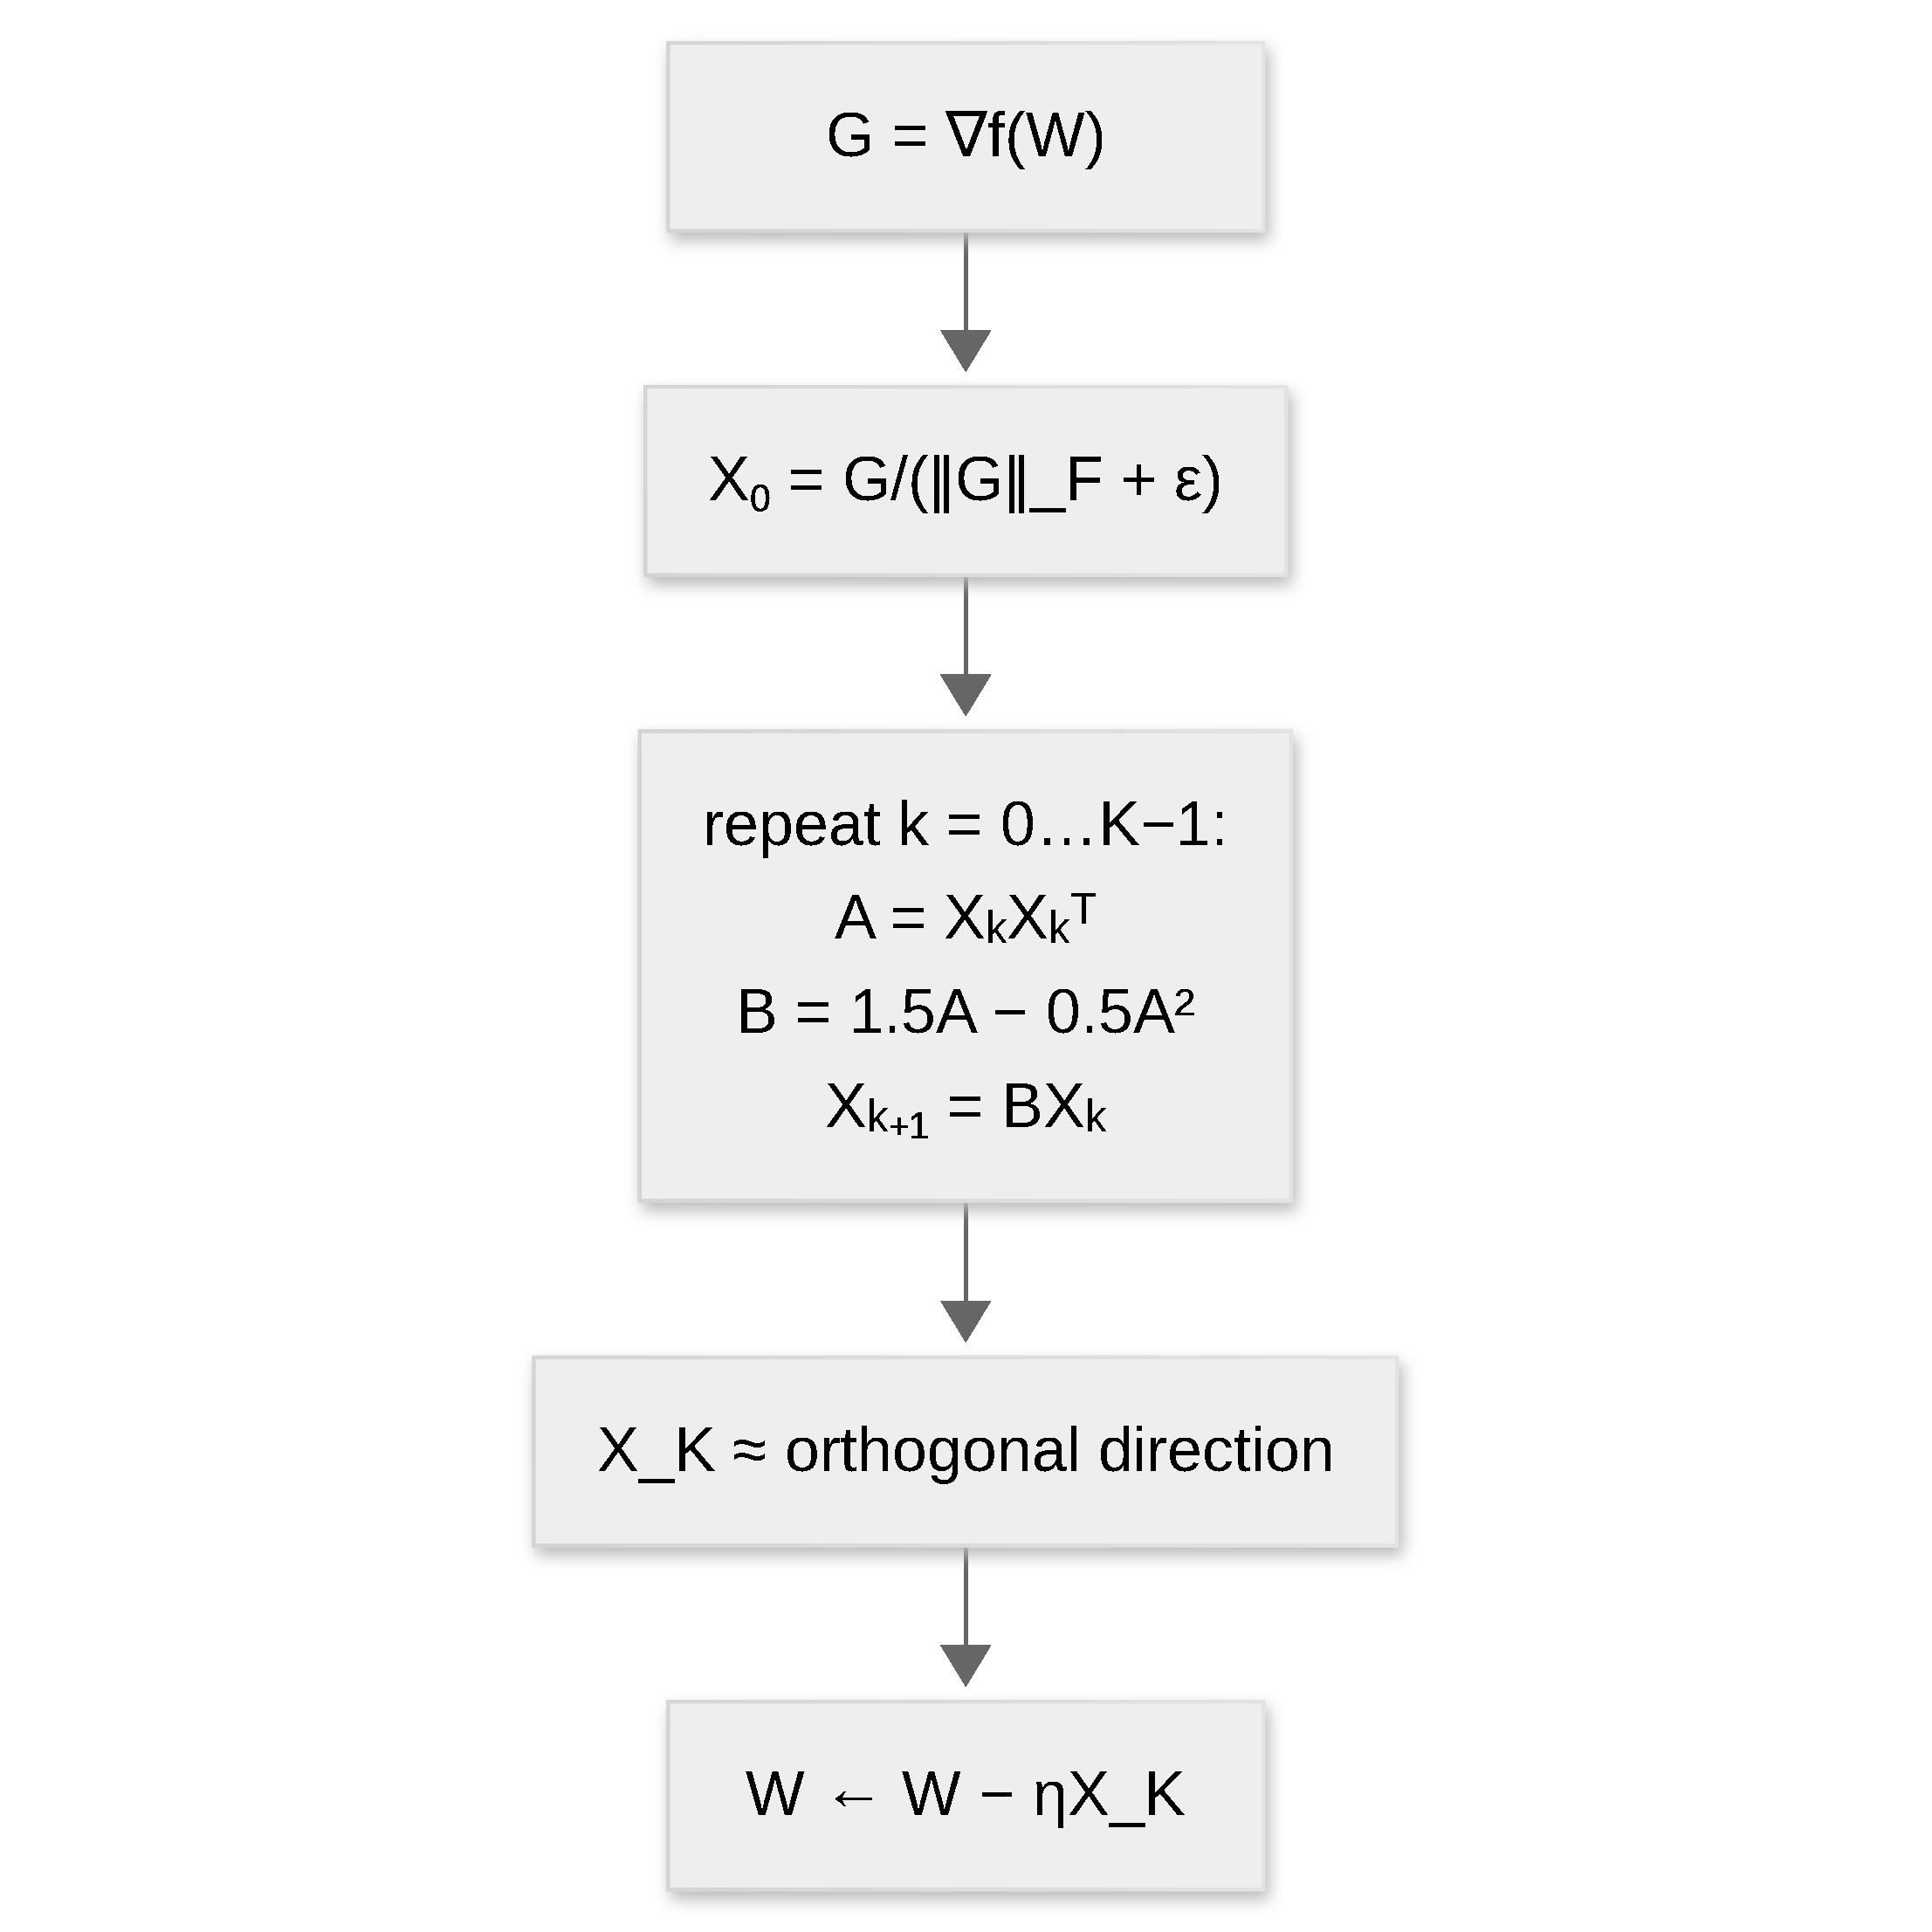
\includegraphics{figures/optimizers/muon.pdf}}
\caption{Step flow of Muon: Frobenius normalization followed by Newton-Schulz iterations that orthogonalize the update direction.}
\label{fig:opt-muon}
\end{figure}
Muon is an \textbf{orthogonality-oriented optimizer} that reshapes update geometry using Newton-Schulz polynomial iterations for orthogonalization. For a 2D parameter matrix $W$ with gradient $G_t$:
\begin{align}
X_0 &= \frac{G_t}{\|G_t\|_F + \epsilon} \quad\text{(normalized gradient)} \\
A_k &= X_k X_k^\top \quad\text{(Gramian)} \\
B_k &= b A_k + c A_k^2 \quad\text{(polynomial step, coefficients $b, c$ from Newton-Schulz)} \\
X_{k+1} &= a X_k + B_k X_k \quad\text{(iteration $k=0,1,\ldots,4$)} \\
W_{t+1} &= W_t - \eta X_K \quad\text{(update with orthogonalized direction)}
\end{align}
Muon performs 5 Newton-Schulz iterations to produce an approximately orthogonal direction, ensuring updates respect geometric constraints. The rationale: orthogonal updates preserve norms during training, avoiding the norm creep observed in momentum-based methods.

\begin{algorithm}[H]
\caption{Muon (Newton-Schulz Orthogonalization)}
\label{alg:muon}
\begin{algorithmic}[1]
\Require Initial parameters $\theta$ (matrices), learning rate $\eta$, Newton-Schulz iters $K$
\Ensure Updated parameters $\theta_T$
\For{each 2D parameter matrix $W$}
    \State $G \gets \nabla f(W)$ \Comment{Gradient}
    \State $X_0 \gets \frac{G}{\|G\|_F + \epsilon}$ \Comment{Normalize gradient by Frobenius norm}
    \For{$k = 0, 1, \ldots, K-1$}
        \State $A_k \gets X_k X_k^\top$ \Comment{Gramian (cost: $O(mn^2)$ or $O(m^2n)$ for tall/wide)}
        \State $B_k \gets (3/2) A_k - (1/2) A_k^2$ \Comment{Newton-Schulz coefficients}
        \State $X_{k+1} \gets B_k X_k$ \Comment{Polynomial step}
    \EndFor
    \State $W \gets W - \eta X_K$ \Comment{Update with orthogonalized direction}
\EndFor
\Return $\theta_T$
\end{algorithmic}
\end{algorithm}

\paragraph{Cons.}
\begin{itemize}[leftmargin=*]
\item Several matrix multiplications per Newton-Schulz iteration; efficient custom kernels are required.
\item Defined only for 2D parameter matrices.
\end{itemize}

\paragraph{Pros.}
\begin{itemize}[leftmargin=*]
\item Orthogonalized updates preserve norms and avoid the norm creep of momentum-based methods.
\item Promising results on large-scale training with fundamentally better-conditioned update geometry.
\end{itemize}

\paragraph{Turbo-Muon (AOL-Preconditioned Orthogonalization).}
\begin{figure}[H]
\centering
\fitfigure{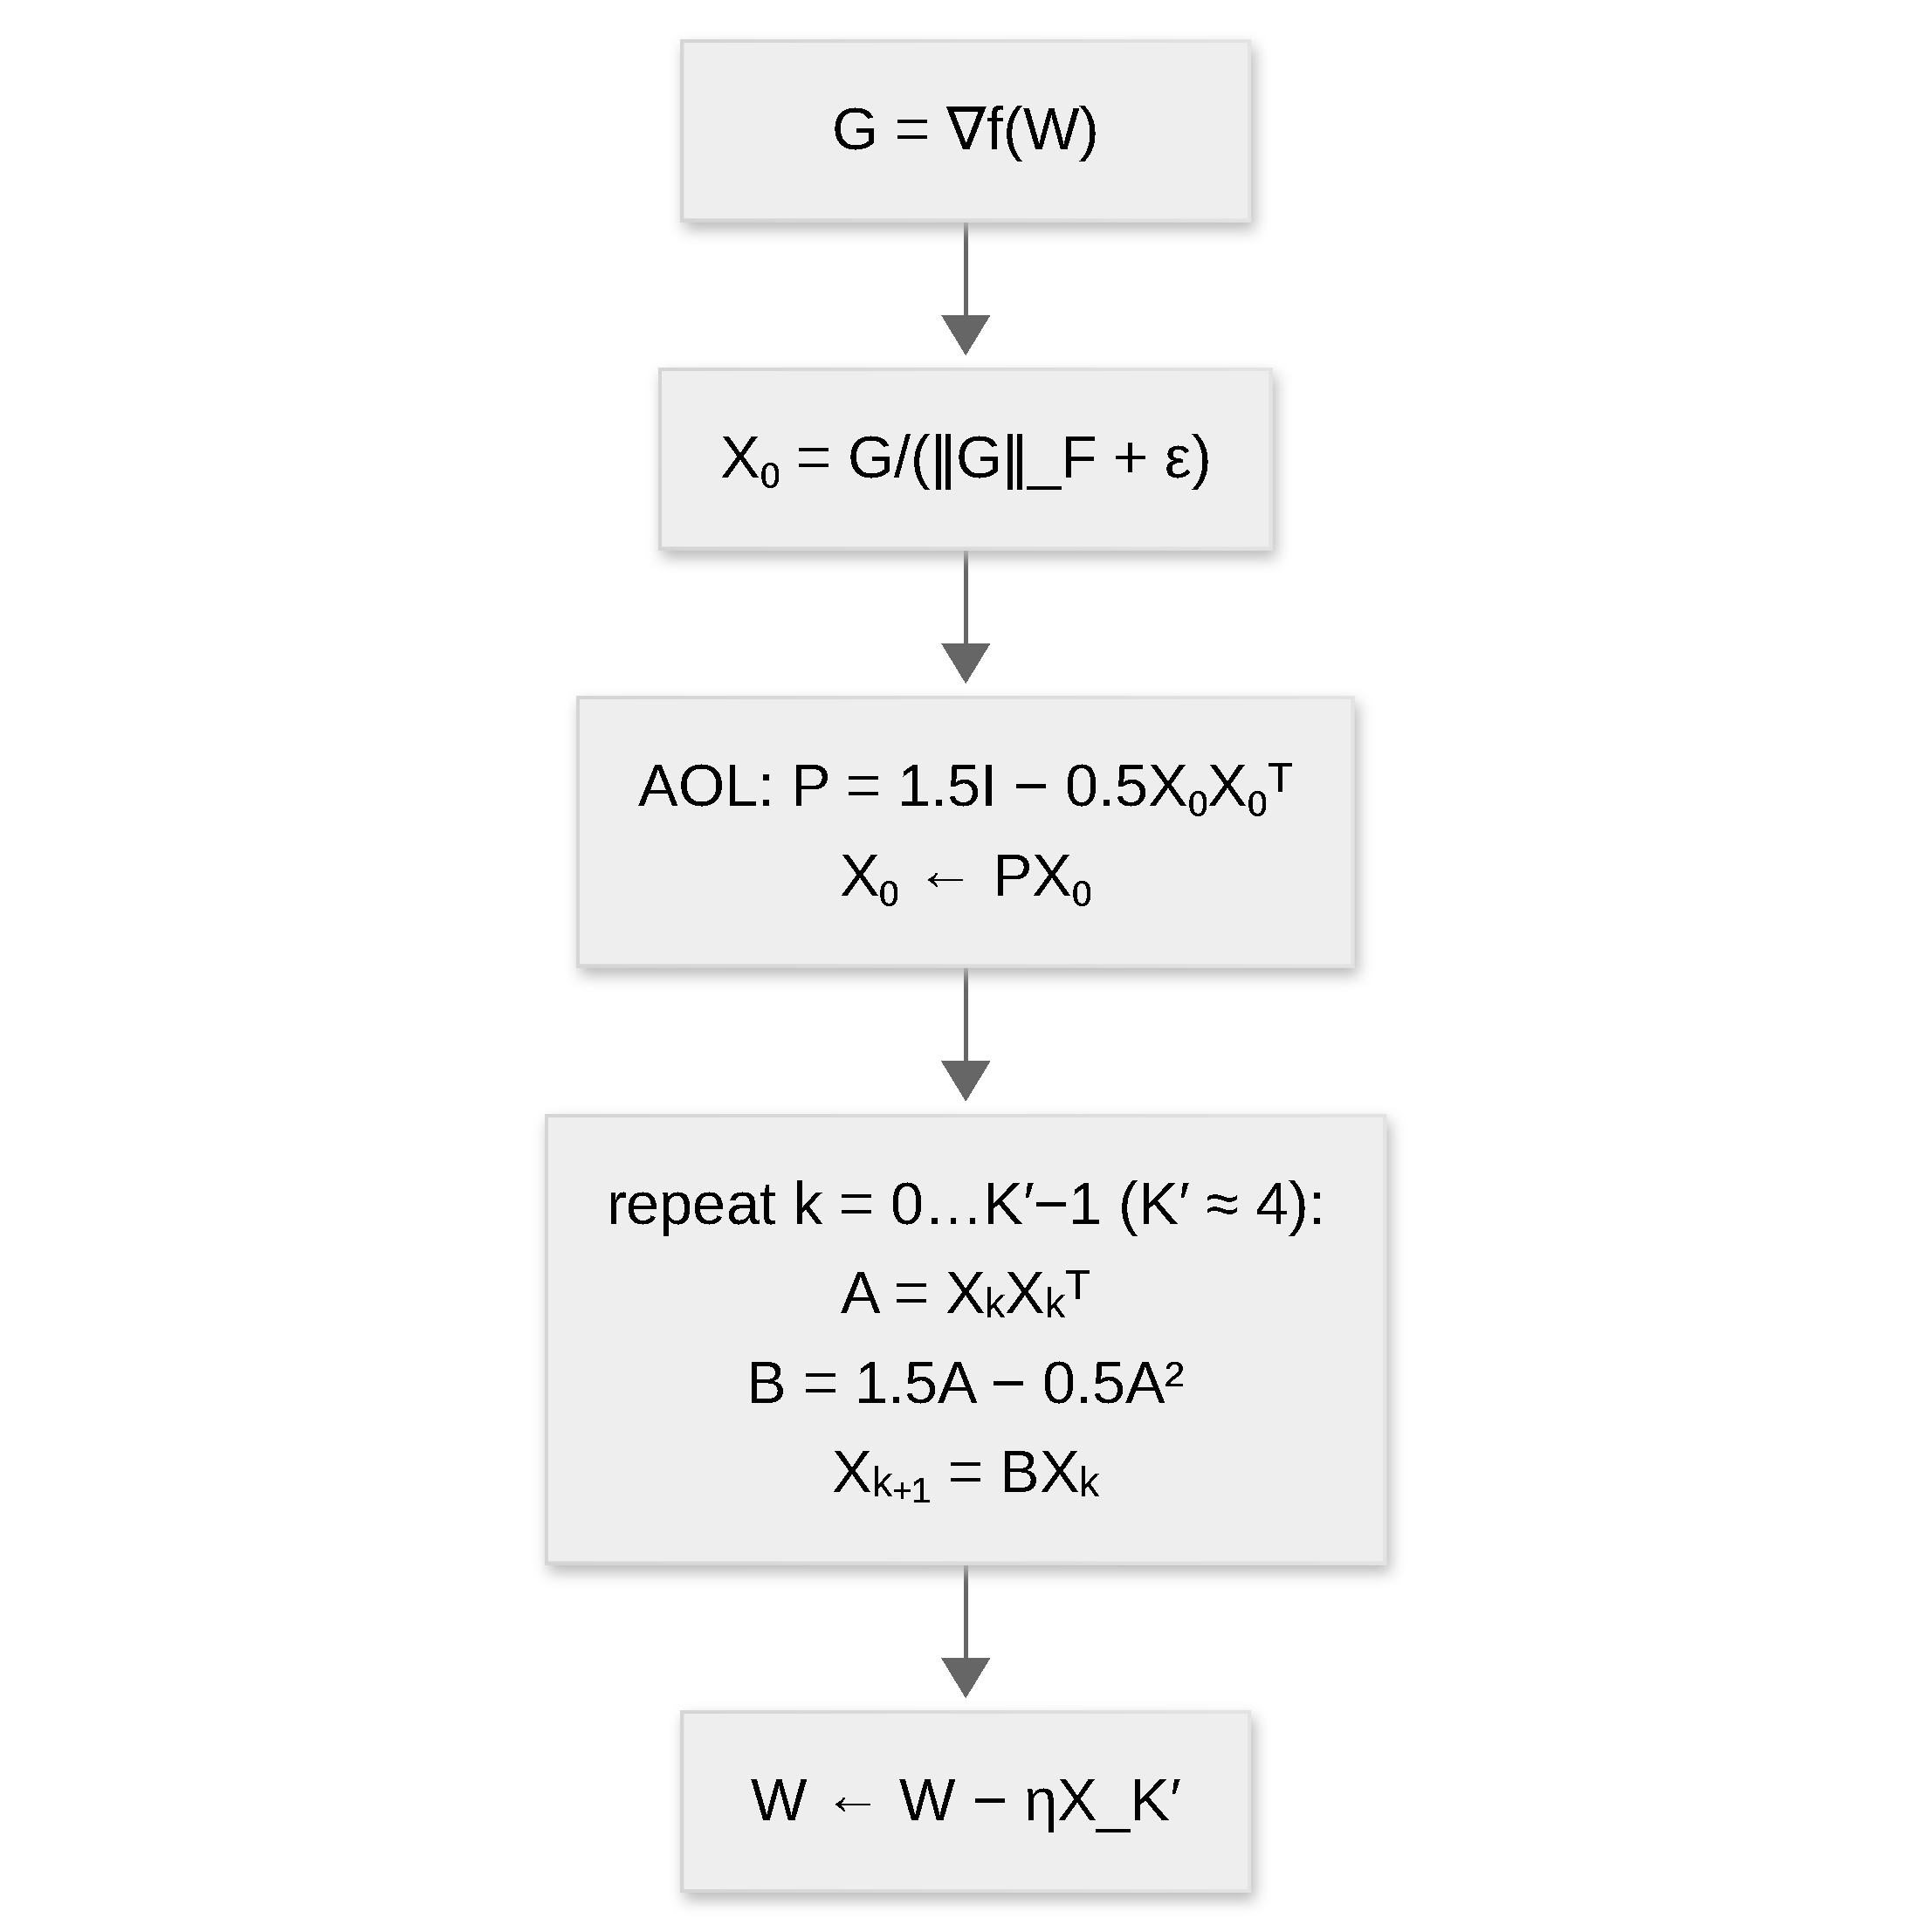
\includegraphics{figures/optimizers/turbo-muon.pdf}}
\caption{Step flow of Turbo-Muon: almost-orthogonal preconditioning (AOL) before the Newton-Schulz iterations, reducing their count.}
\label{fig:opt-turbo-muon}
\end{figure}
Turbo-Muon adds an \textbf{almost-orthogonal preconditioning} (AOL) step before the Newton-Schulz iterations. The preconditioner $P = 1.5I - 0.5X_0X_0^\top$ is applied to the normalized gradient, reducing the number of required orthogonalization steps to four while preserving the orthogonalized update geometry.

\begin{algorithm}[H]
\caption{Turbo-Muon (AOL-Preconditioned Orthogonalization)}
\label{alg:turbo-muon}
\begin{algorithmic}[1]
\Require Initial parameters $\theta$ (matrices), learning rate $\eta$, Newton-Schulz iters $K'$ (typically 4)
\Ensure Updated parameters $\theta_T$
\For{each 2D parameter matrix $W$}
    \State $G \gets \nabla f(W)$ \Comment{Gradient}
    \State $X_0 \gets \frac{G}{\|G\|_F + \epsilon}$ \Comment{Normalize gradient}
    \State \textbf{AOL (Almost-Orthogonal preconditioner):} \Comment{Preconditioning step}
    \State $P \gets (1.5 I - 0.5 X_0 X_0^\top)$ \Comment{Preconditioning matrix}
    \State $X_0 \gets P X_0$ \Comment{Preconditioned start}
    \For{$k = 0, 1, \ldots, K'-1$}
        \State $A_k \gets X_k X_k^\top$
        \State $B_k \gets (3/2) A_k - (1/2) A_k^2$
        \State $X_{k+1} \gets B_k X_k$ \Comment{Reduced iterations due to AOL preconditioning}
    \EndFor
    \State $W \gets W - \eta X_{K'}$ \Comment{Update with preconditioned orthogonalized direction}
\EndFor
\Return $\theta_T$
\end{algorithmic}
\end{algorithm}

\paragraph{Cons.}
\begin{itemize}[leftmargin=*]
\item Still compute-heavy; AOL adds a preconditioning matrix multiplication.
\item Requires the same custom-kernel support as Muon.
\end{itemize}

\paragraph{Pros.}
\begin{itemize}[leftmargin=*]
\item AOL reduces the Newton-Schulz iteration count (typically five to four).
\item Retains orthogonalized update geometry at lower iteration cost.
\end{itemize}

\paragraph{AF-Muon (AdamW-Free Tied-Embedding Muon).}
\begin{figure}[H]
\centering
\fitfigure{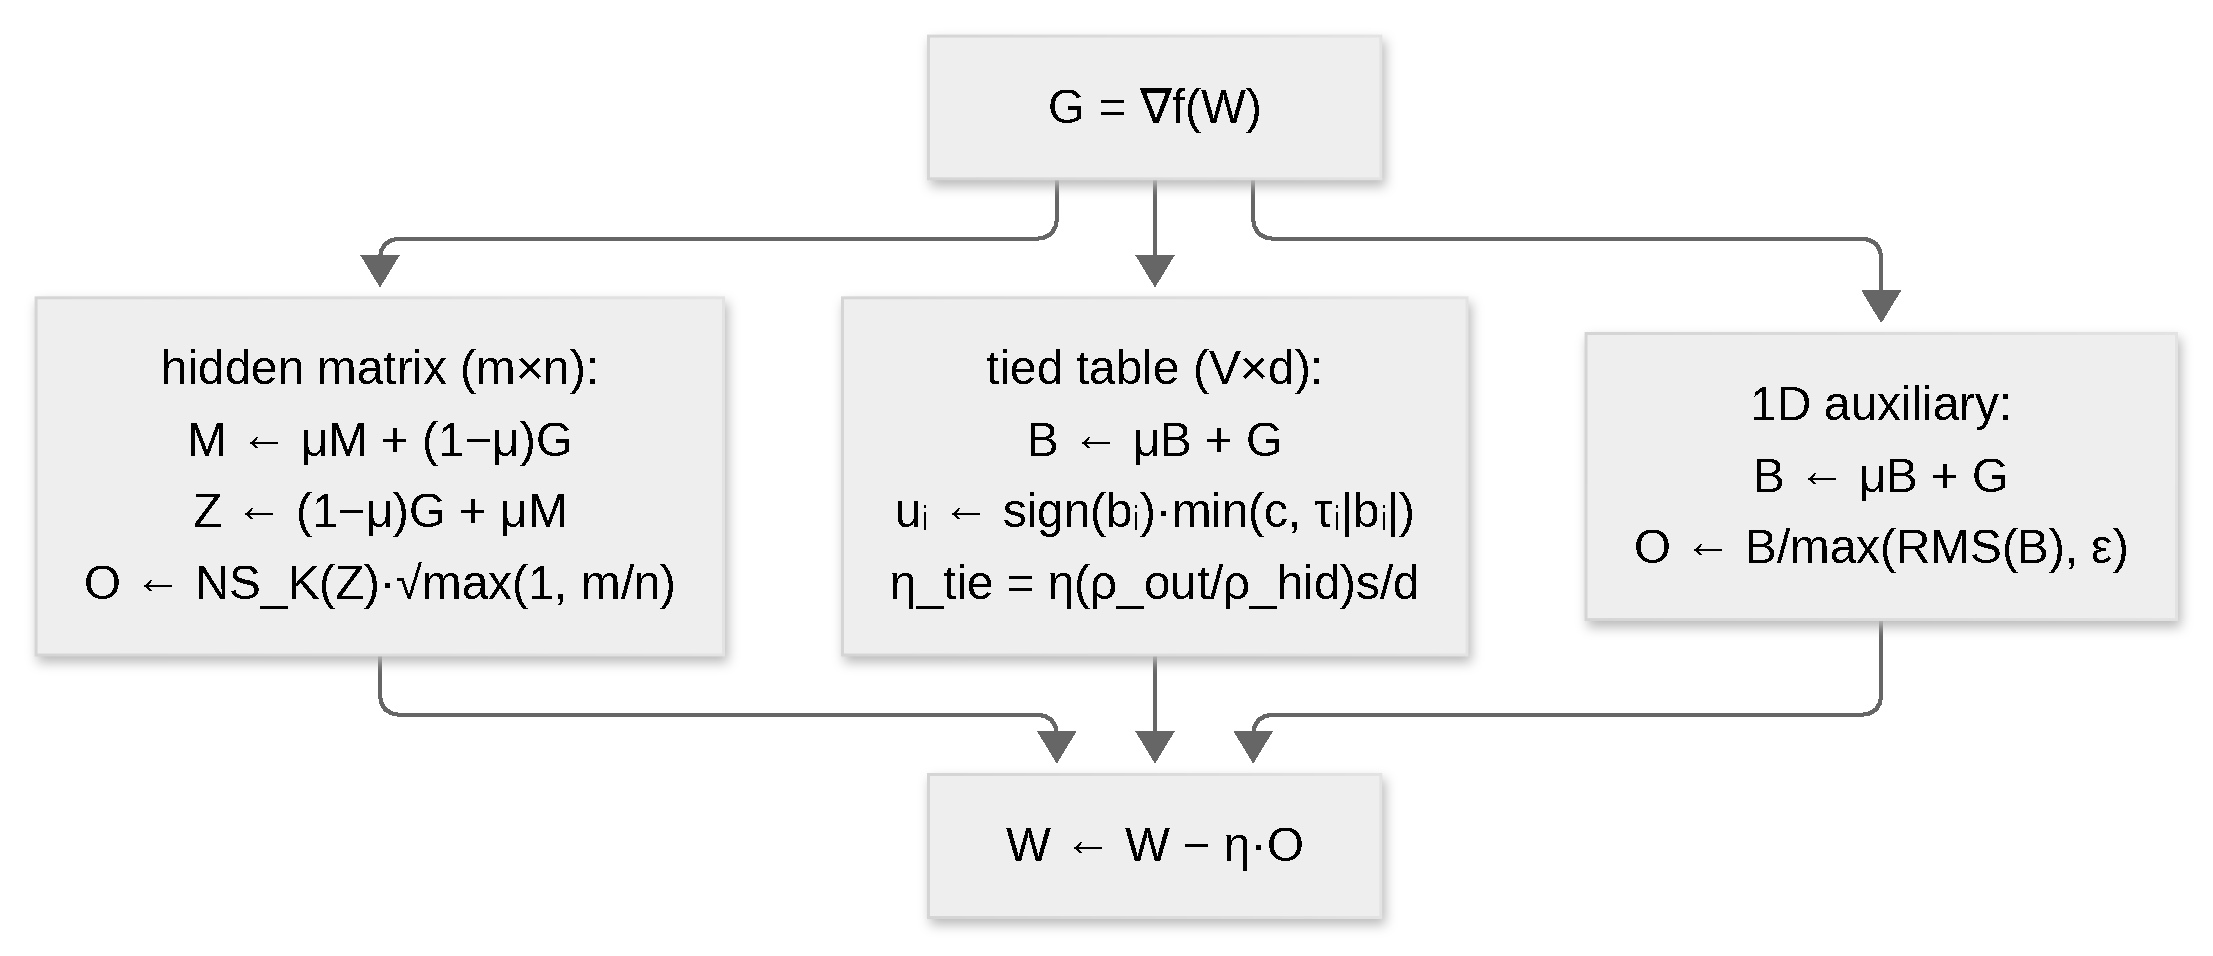
\includegraphics{figures/optimizers/af-muon.pdf}}
\caption{Step flow of AF-Muon: Muon's spectral update for hidden matrices, a support-aware finite-cap clipped-row LMO for the tied vocabulary table, and RMS-normalized updates for one-dimensional auxiliary parameters, all with a single first-moment buffer.}
\label{fig:opt-af-muon}
\end{figure}
AF-Muon is an \textbf{AdamW-free extension of Muon} that removes the auxiliary AdamW fallback of the Hybrid Muon recipe by giving every parameter class its own norm-constrained geometry. Hidden matrices keep the spectral update with a Nesterov signal; the vocabulary table, which simultaneously receives sparse input-lookup and dense output-softmax gradients, is updated row by row with a \emph{support-aware finite-cap linear minimization oracle}; one-dimensional auxiliary tensors receive an RMS-normalized update. No parameter class carries second-moment state, so a single first-moment buffer per parameter replaces the AdamW state of the hybrid recipe, which the authors report as roughly 20\% less optimizer-state memory at matched training.

For the tied table $W \in \mathbb{R}^{V \times d}$ with momentum row $b_i$, the oracle solves the row problem
\begin{align}
u_i &= \operatorname{sign}(b_i) \odot \min\left(c\,\mathbf{1},\ \tau_i\,|b_i|\right), \\
\|u_i\|_2^2 &= \min\left(d,\ c^2\,\bigl|\operatorname{supp}(b_i)\bigr|\right),
\end{align}
where the per-row scale $\tau_i$ is obtained by bisection in FP32 over complete-row chunks. Rows whose support cannot fill the row-$\ell_2$ radius saturate every useful coordinate at the cap $c$, so sparse lookup rows are handled without inflating absent coordinates. The cap interpolates between two known endpoints: $c = 1$ recovers the SCION-style Sign update and $c \geq \sqrt{d}$ reduces to a row-RMS update. The tied step size is $\eta_{tie} = \eta_M (\rho_{out}/\rho_{hid})\, s / d$; the paper's main setting is $c = 3$ and $s = 0.5$ with $\rho_{out}/\rho_{hid} = 60$, and its diagnostics report the finite cap active on under 0.3\% of coordinates while affecting most rows.

\begin{algorithm}[H]
\caption{AF-Muon (AdamW-Free Tied-Embedding Muon)}
\label{alg:af-muon}
\begin{algorithmic}[1]
\Require Initial parameters $\theta$, matrix LR $\eta_M$, vector LR $\eta_{vec}$, momentum $\mu$, matrix weight decay $\lambda_M$, tied scale $s$, cap $c$, radii $\rho_{out}, \rho_{hid}$, Newton-Schulz iters $K$
\Ensure Updated parameters $\theta_T$
\For{each parameter tensor $W$ with gradient $G_t$}
    \If{$W$ is a hidden matrix in $\mathbb{R}^{m \times n}$}
        \State $M_t \gets \mu M_{t-1} + (1-\mu) G_t$ \Comment{First moment}
        \State $Z_t \gets (1-\mu) G_t + \mu M_t$ \Comment{Nesterov signal}
        \State $O_t \gets \mathrm{NS}_K(Z_t)\sqrt{\max(1, m/n)}$ \Comment{Spectral update}
        \State $W_t \gets (1 - \eta_M \lambda_M) W_{t-1} - \eta_M O_t$
    \ElsIf{$W \in \mathbb{R}^{V \times d}$ is the tied vocabulary table}
        \State $B_t \gets \mu B_{t-1} + G_t$ \Comment{Unnormalized first moment}
        \State $\eta_{tie,t} \gets \eta_M (\rho_{out}/\rho_{hid}) s / d$
        \For{each row $i = 1, \ldots, V$}
            \State $u_i \gets L_c\bigl(\mathrm{row}_i(B_t)\bigr)$ \Comment{Capped-row LMO}
        \EndFor
        \State $W_t \gets W_{t-1} - \eta_{tie,t} U$
    \Else
        \State $B_t \gets \mu B_{t-1} + G_t$ \Comment{$1$D auxiliary tensor}
        \State $O_t \gets B_t / \max(\mathrm{RMS}(B_t), \epsilon)$
        \State $W_t \gets W_{t-1} - \eta_{vec} O_t$
    \EndIf
\EndFor
\Return $\theta_T$
\end{algorithmic}
\end{algorithm}

\paragraph{Cons.}
\begin{itemize}[leftmargin=*]
\item Every parameter must be assigned an explicit role (matrix, tied table, or vector); an untied output head or an extra embedding table is not a tied-table block.
\item The tied-table oracle requires a per-row bisection with complete-row chunking; the paper reports roughly 1\% median step-time overhead at matched training.
\item The tied-table claim is established for tied-vocabulary models; frontier-scale pretraining and universal endpoint superiority are not claimed.
\end{itemize}

\paragraph{Pros.}
\begin{itemize}[leftmargin=*]
\item AdamW-free: one first-moment buffer per parameter and no second-moment state, reported as roughly 20\% less optimizer-state memory than Hybrid Muon.
\item The finite cap preserves within-row magnitudes while bounding coordinate concentration, and recovers Sign ($c=1$) and row-RMS ($c \geq \sqrt{d}$) as limit cases.
\item Improves mean validation loss and perplexity over both Hybrid Muon and a SCION-style Sign endpoint across nine tied-token settings spanning text, image-token, protein, MoE, and encoder-decoder models.
\end{itemize}

\small
\begin{longtable}{L{2.5cm}L{3.5cm}L{2.3cm}L{5.0cm}}
\toprule
\textbf{Group} & \textbf{Methods} & \textbf{Primary Goal} & \textbf{Interpretation from the Survey} \\
\midrule
\endhead
Classical baseline & SGD, AdamW, RAdam & stability and reference baselines & These define the comparison floor for newer optimizer claims. \\
Momentum redesign & Adan, AdEMAMix, MARS, Cautious AdamW & faster or safer first-order adaptation & Best when convergence speed or noisy-gradient stability is the main concern. \\
Large-batch and schedule simplification & LAMB, Schedule-Free AdamW & operational robustness at scale & Reduce brittleness from batch-size growth or schedule engineering. \\
Memory-efficient & Adafactor, GaLore, APOLLO, APOLLO-Mini, Q-APOLLO, Lion & optimizer-state reduction & Most useful when VRAM is dominated by optimizer state rather than activations; APOLLO-family methods replace dense AdamW moments with projected or quantized structured scaling. \\
Curvature-aware & Shampoo, SOAP, Sophia & better conditioning & Prefer when richer geometry is worth implementation and compute overhead. \\
Geometry-oriented & Muon, Turbo-Muon, AF-Muon & orthogonalized update structure & Specialized options for matrix geometry and representation shaping; AF-Muon assigns the tied vocabulary table a capped-row table geometry and one-dimensional parameters an RMS update, with no AdamW auxiliary state. \\
\bottomrule
\end{longtable}
\normalsize

\section{Dense, Recurrent, and Memory-Augmented Transformers}
\label{sec:annex-transformer}

This annex synthesizes the dense, recurrent, and memory-augmented transformer families. The field has evolved toward several primary paradigms: dense global attention with variants, key-value head compression via grouped-query attention, recurrent state compression with decay, selective state-space models, continuous-depth numerical integration, and memory-augmented architectures. Understanding this taxonomy illuminates fundamental tradeoffs between expressiveness, computational cost, memory footprint, and deployment simplicity.

\subsection{Dense Attention Baselines: Standard and Sigmoid}

\subsubsection{Standard Softmax Attention}

\begin{figure}[H]
\centering
\fitfigure{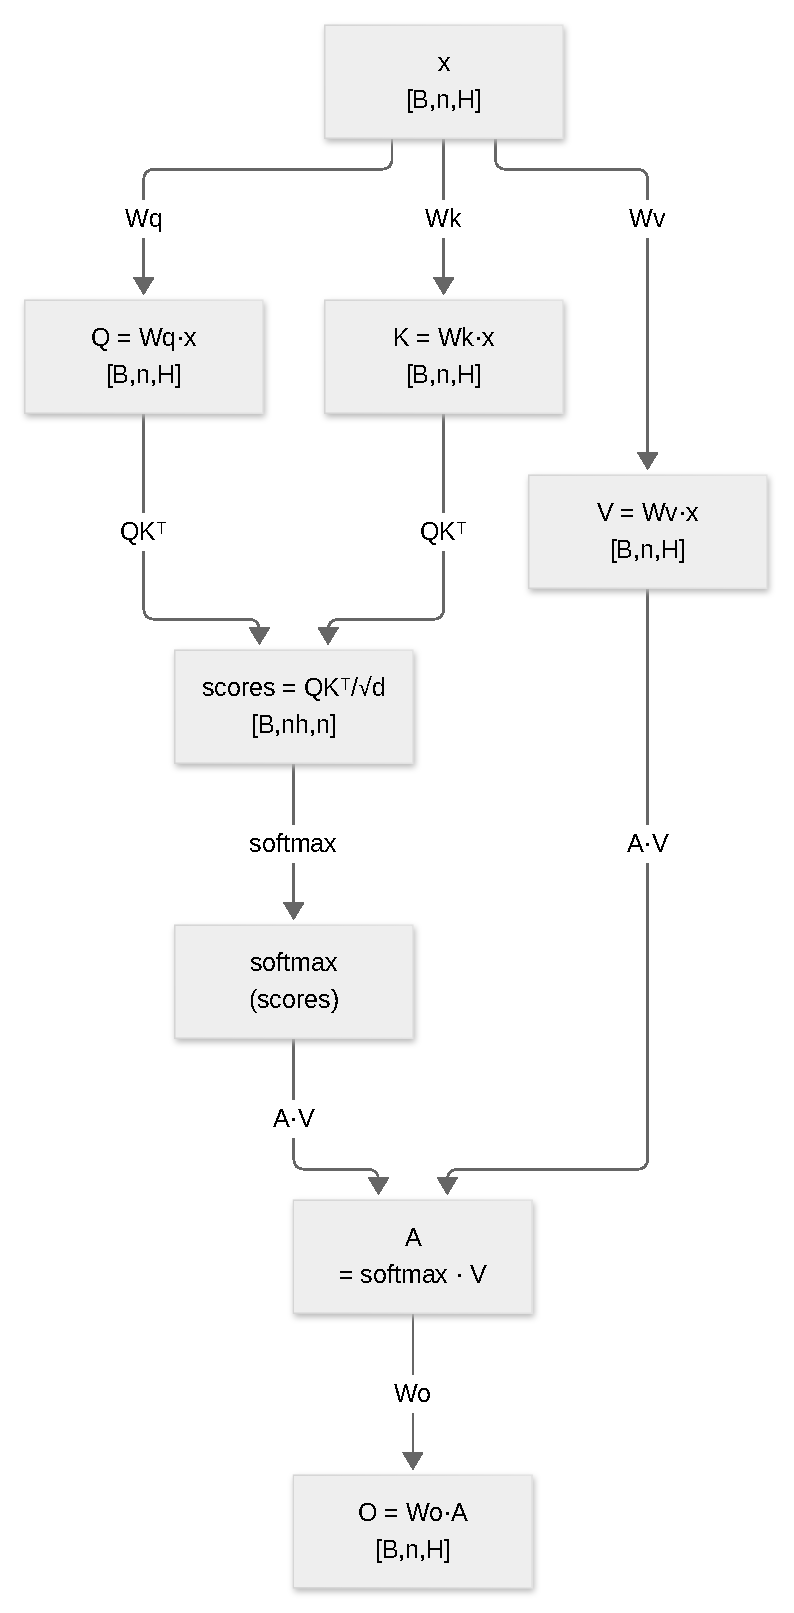
\includegraphics{figures/mixers/standard.pdf}}
\caption{Dataflow of standard softmax attention: parallel Q/K/V projections, scaled dot-product scores, row-wise softmax, and output projection.}
\label{fig:mixer-standard}
\end{figure}
Standard multi-head self-attention \citep{vaswani_attention_2017} computes scaled dot-product similarity between token embeddings:

\begin{algorithmic}[1]
\State \textbf{Input:} Query matrix $\mathbf{Q} \in \mathbb{R}^{n \times d}$, Key matrix $\mathbf{K} \in \mathbb{R}^{n \times d}$, Value matrix $\mathbf{V} \in \mathbb{R}^{n \times d}$
\State $\text{scores} \gets \frac{\mathbf{Q}\mathbf{K}^\top}{\sqrt{d}} \in \mathbb{R}^{n \times n}$ \Comment{compute pairwise similarities}
\State $\text{attention\_weights} \gets \texttt{softmax}(\text{scores}, \text{axis}=1) \in \mathbb{R}^{n \times n}$ \Comment{normalize across keys}
\State \textbf{Output:} $\mathbf{Y} = \text{attention\_weights} \cdot \mathbf{V} \in \mathbb{R}^{n \times d}$ \Comment{weighted value combination}
\end{algorithmic}

For autoregressive generation, KV caching stores past keys and values to avoid $\mathcal{O}(n^2)$ recomputation. However, this linearly growing cache occupies $\sim n \cdot d_{\text{hidden}}$ bytes, which can consume hundreds of gigabytes for billion-parameter models. Standard attention achieves \textbf{perfect expressiveness} within the context window---any token can attend to any other token with learned weights---but pays the price of dense computation.

\begin{itemize}[leftmargin=*]
    \item \textbf{Training complexity}: $\mathcal{O}(n^2 \cdot d)$ time, $\mathcal{O}(n^2)$ space (attention matrix materialization).
    \item \textbf{Inference complexity}: $\mathcal{O}(n)$ time per token, $\mathcal{O}(n)$ space (KV cache).
    \item \textbf{Strengths}: Unparalleled expressiveness; perfect history recall; highly parallelizable.
    \item \textbf{Weaknesses}: Quadratic bottleneck prohibits very long contexts; KV cache dominates memory during generation.
\end{itemize}

\subsubsection{Sigmoid Attention}

\begin{figure}[H]
\centering
\fitfigure{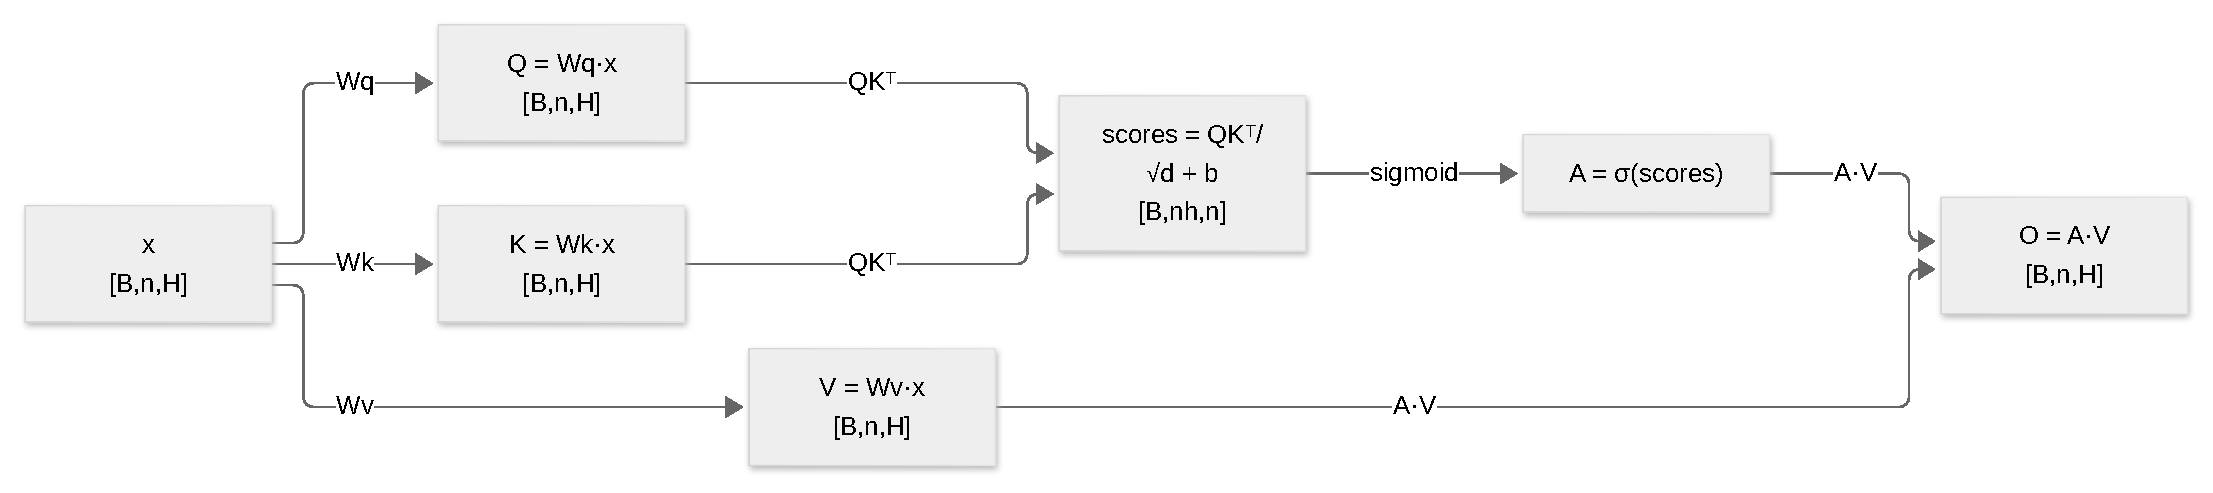
\includegraphics{figures/mixers/sigmoid.pdf}}
\caption{Dataflow of sigmoid attention: an element-wise sigmoid replaces the row-wise softmax, so attention weights need not sum to one.}
\label{fig:mixer-sigmoid}
\end{figure}
Sigmoid attention replaces row-wise softmax with element-wise sigmoid activation \citep{ramapuram_theory_2024}:

\begin{algorithmic}[1]
\State \textbf{Input:} $\mathbf{Q}, \mathbf{K}, \mathbf{V}$ as above, learnable bias $\mathbf{b} \in \mathbb{R}^{n \times n}$
\State $\text{logits} \gets \frac{\mathbf{Q}\mathbf{K}^\top}{\sqrt{d}} + \mathbf{b}$
\State $\text{attention\_weights} \gets \sigma(\text{logits})$ \Comment{element-wise sigmoid, not softmax}
\State \textbf{Output:} $\mathbf{Y} = \text{attention\_weights} \odot \mathbf{V}$
\end{algorithmic}

Unlike softmax, sigmoid does not enforce a probability distribution (weights need not sum to 1), enabling stronger token independence. Theoretical analysis via mixture-of-experts shows sigmoid achieves superior sample complexity: $\mathcal{O}(n^{-0.51})$ convergence for ReLU experts versus softmax's $\mathcal{O}(n^{-0.24})$. However, empirical training revealed gradient instabilities at scale. The remedy is \textbf{hybrid-norm}---adding normalization after the attention output---which stabilizes gradients without sacrificing the theoretical benefits of element-wise gating.

\begin{itemize}[leftmargin=*]
    \item \textbf{Training complexity}: $\mathcal{O}(n^2 \cdot d)$ (identical to standard), but element-wise operations enable 17\% inference speedup via FlashSigmoid.
    \item \textbf{Inference complexity}: $\mathcal{O}(n)$ per token with KV cache (asymptotically same, but lower constant factors).
    \item \textbf{Strengths}: Overcomes zero-sum competition; avoids row-wise synchronization; hardware-friendly implementation.
    \item \textbf{Weaknesses}: Requires careful stabilization (hybrid-norm); training instability at large scales without auxiliary loss.
\end{itemize}

\subsubsection{Grouped-Query Attention (GQA)}

\begin{figure}[H]
\centering
\fitfigure{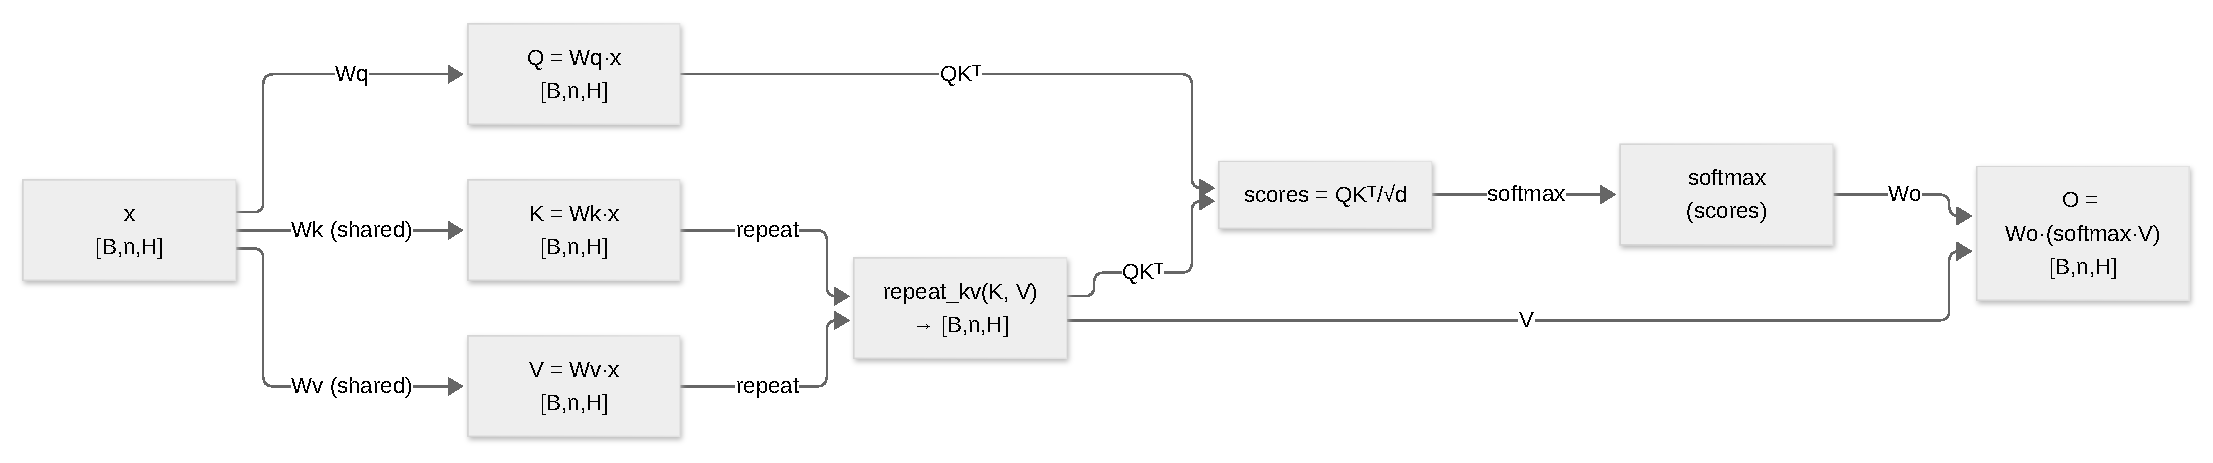
\includegraphics{figures/mixers/gqa.pdf}}
\caption{Dataflow of grouped-query attention: keys and values are projected to fewer heads, expanded by repeat-interleave, and shared across each group of query heads.}
\label{fig:mixer-gqa}
\end{figure}
Grouped-query attention \citep{ainslie_gqa_2023} bridges multi-head attention (MHA) and multi-query attention (MQA) by partitioning query heads into groups, each sharing a single key-value head. If $h$ is the total number of attention heads, $h_k$ is the number of key-value heads, and $G = h / h_k$ is the group size, then every group of $G$ query heads shares one KV head:

\begin{algorithmic}[1]
\State \textbf{Input:} $\mathbf{Q} \in \mathbb{R}^{n \times h \cdot d_h}$, $\mathbf{K} \in \mathbb{R}^{n \times h_k \cdot d_h}$, $\mathbf{V} \in \mathbb{R}^{n \times h_k \cdot d_h}$
\State $\mathbf{K}_{\text{full}} \gets \texttt{repeat\_interleave}(\mathbf{K}, G)$ \Comment{expand from $h_k$ to $h$ heads}
\State $\mathbf{V}_{\text{full}} \gets \texttt{repeat\_interleave}(\mathbf{V}, G)$
\State $\text{scores} \gets \frac{\mathbf{Q}\mathbf{K}_{\text{full}}^\top}{\sqrt{d_h}} \in \mathbb{R}^{n \times n}$ \Comment{standard dot product after expansion}
\State $\text{attention\_weights} \gets \texttt{softmax}(\text{scores}, \text{axis}=1)$
\State \textbf{Output:} $\mathbf{Y} = \text{attention\_weights} \cdot \mathbf{V}_{\text{full}} \in \mathbb{R}^{n \times h \cdot d_h}$
\end{algorithmic}

GQA interpolates smoothly between MHA ($h_k = h$, $G = 1$) and MQA ($h_k = 1$, $G = h$). The key advantage is a tunable tradeoff between KV-cache footprint and representational capacity. Each additional KV head consumes $2 \cdot d_h \cdot n$ extra bytes in the cache, so reducing $h_k$ yields proportional memory savings.

\begin{itemize}[leftmargin=*]
    \item \textbf{Training complexity}: $\mathcal{O}(n^2 \cdot h \cdot d_h)$ (identical to MHA after head expansion).
    \item \textbf{Inference complexity}: $\mathcal{O}(n)$ per token, $\mathcal{O}(h_k \cdot n \cdot d_h)$ KV-cache space.
    \item \textbf{Strengths}: Flexible head-count tradeoff; proven at scale (Llama 2 \& 3 use $h_k = 8$ KV heads with $h = 32$ query heads); reduces KV-cache by $G \times$; supports fast inference with FlashAttention.
    \item \textbf{Weaknesses}: Fewer KV heads can reduce representational capacity in small models; requiring $h_k$ to divide $h$ constrains architectural choices.
\end{itemize}

\subsection{Recurrent and Retentive Architectures}

\subsubsection{Retentive Networks (RetNet)}

\begin{figure}[H]
\centering
\fitfigure{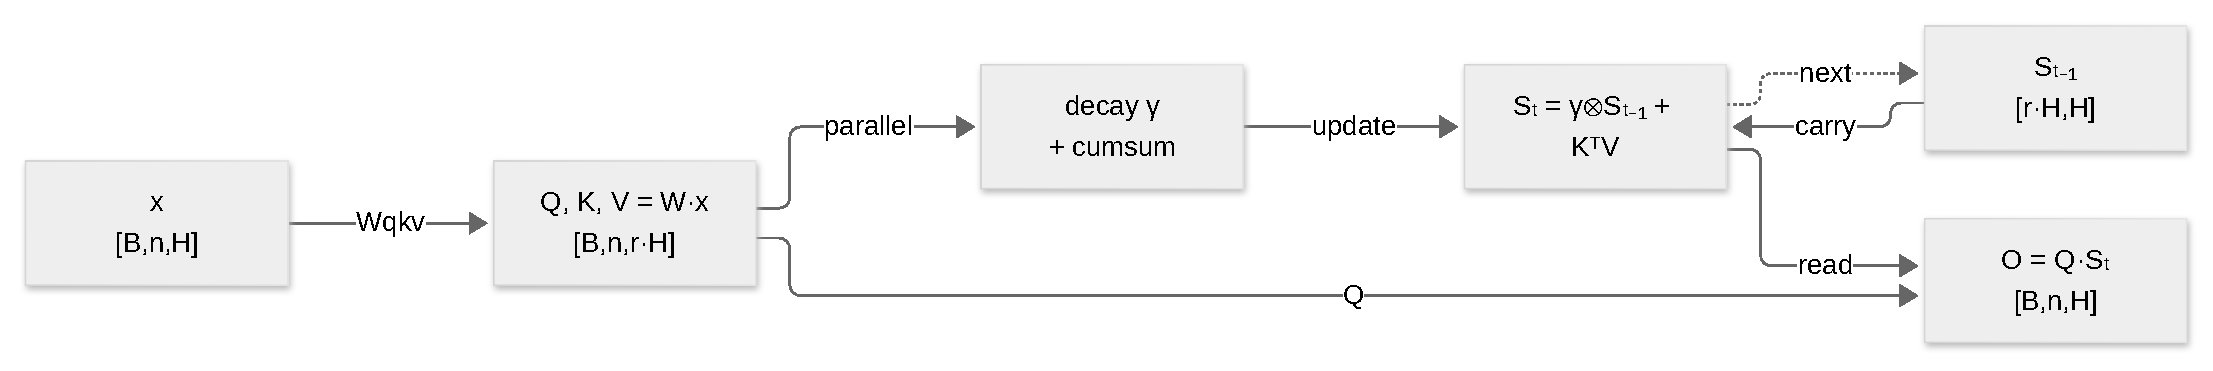
\includegraphics{figures/mixers/retnet.pdf}}
\caption{Dataflow of RetNet: parallel Q/K/V projections feed a decayed state recurrence; the state carries across steps and the output reads it with the query.}
\label{fig:mixer-retnet}
\end{figure}
RetNet \citep{sun_retentive_2023} unifies three computation paradigms: parallel training, recurrent inference, and chunkwise deployment. Its core innovation is the \textbf{retention mechanism}, which uses a fixed exponential decay matrix to model temporal importance:

\begin{algorithmic}[1]
\State \textbf{Parallel (training) form:}
\State $\text{decay\_matrix}[i,j] \gets \gamma^{i-j}$ for $i \geq j$, else $0$ \Comment{causal exponential decay}
\State $\text{decay\_matrix}[i,j] \gets 0$ for $i < j$ \Comment{causal masking}
\State $\mathbf{Y}_{\text{parallel}} \gets (\mathbf{Q}\mathbf{K}^\top \odot \text{decay\_matrix}) \mathbf{V}$ \Comment{element-wise multiplication with decay}
\end{algorithmic}

\begin{algorithmic}[1]
\State \textbf{Recurrent (inference) form:}
\For{$t = 1, \ldots, n$}
    \State $\mathbf{s}_t \gets \gamma \mathbf{s}_{t-1} + \mathbf{k}_t \mathbf{v}_t^\top$ \Comment{state update with decay}
    \State $\mathbf{y}_t \gets \mathbf{q}_t \mathbf{s}_t$ \Comment{output via query-state interaction}
\EndFor
\end{algorithmic}

The decay scalar $\gamma \in (0,1)$ controls the temporal window. RetNet uses \textbf{multi-scale retention} with different $\gamma$ values per head (e.g., $\gamma = 1 - 2^{-5}, 1 - 2^{-6}, \ldots$), allowing short-term and long-term dependencies simultaneously. Chunkwise recurrent mode divides sequences into chunks, processes each chunk in parallel, and threads a recurrent state between chunks.

\begin{itemize}[leftmargin=*]
    \item \textbf{Training complexity}: $\mathcal{O}(n^2 \cdot d)$ (parallel), or $\mathcal{O}(n \cdot c \cdot d)$ (chunkwise recurrent with chunk size $c$).
    \item \textbf{Inference complexity}: $\mathcal{O}(1)$ per token, $\mathcal{O}(d^2)$ state space (fixed matrix).
    \item \textbf{Strengths}: Constant-time inference; triple computation paradigm; multi-scale consolidation.
    \item \textbf{Weaknesses}: Fixed decay imposes rigid inductive bias; may truncate learned long-range patterns.
\end{itemize}

\subsubsection{Mamba: Selective State-Space Models}

\begin{figure}[H]
\centering
\fitfigure{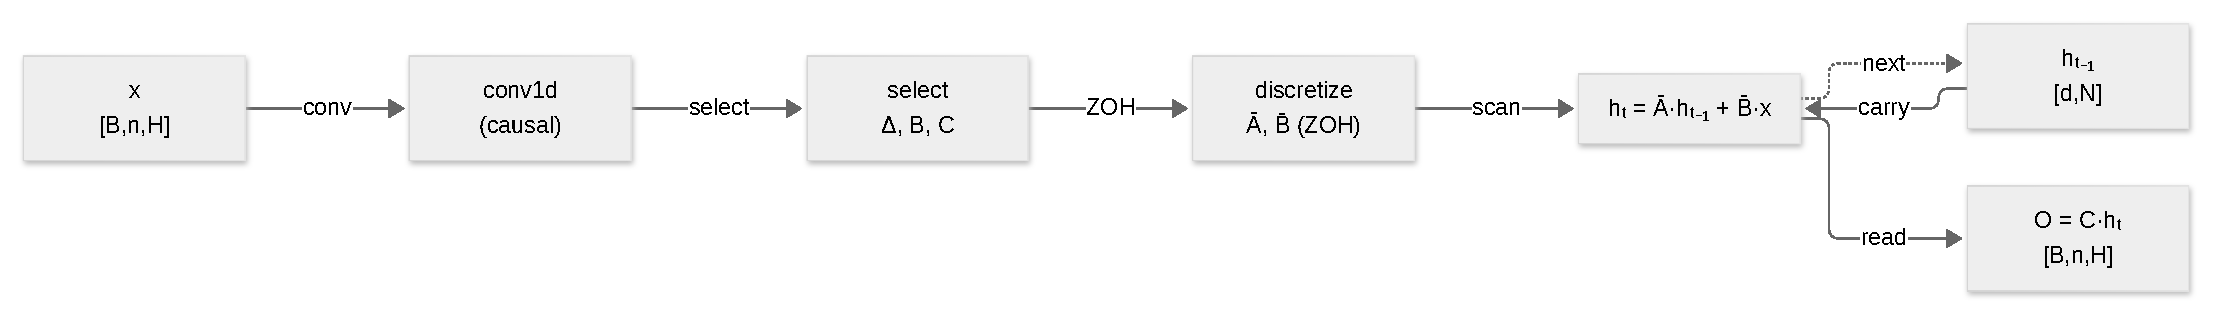
\includegraphics{figures/mixers/mamba.pdf}}
\caption{Dataflow of Mamba: a causal convolution feeds input-dependent $\Delta$, $B$, $C$ selections, ZOH discretization, and a selective state-space scan whose state carries across steps.}
\label{fig:mixer-mamba}
\end{figure}
Mamba \citep{gu_mamba_2023} frames recurrence as a continuous-time dynamical system with input-dependent parameters, achieving both linear training and constant-time inference:

\begin{algorithmic}[1]
\State \textbf{Continuous dynamics:} $h'(t) = \mathbf{A} h(t) + \mathbf{B} x(t)$, \quad $y(t) = \mathbf{C} h(t)$
\State \textbf{Discretization with step size $\Delta_t$:}
\State $\bar{\mathbf{A}}_t \gets \exp(\Delta_t \mathbf{A})$
\State $\bar{\mathbf{B}}_t \gets (\Delta_t \mathbf{A})^{-1} (\exp(\Delta_t \mathbf{A}) - \mathbf{I}) \Delta_t \mathbf{B}_t$
\State \textbf{Recurrent update:}
\For{$t = 1, \ldots, n$}
    \State $\Delta_t \gets \text{softplus}(\text{Linear}(x_t))$ \Comment{input-dependent step size}
    \State $\mathbf{B}_t \gets \text{Linear}(x_t)$, \quad $\mathbf{C}_t \gets \text{Linear}(x_t)$ \Comment{input-dependent projection matrices}
    \State $h_t \gets \bar{\mathbf{A}}_t h_{t-1} + \bar{\mathbf{B}}_t x_t$ \Comment{state transition}
    \State $y_t \gets \mathbf{C}_t h_t$ \Comment{output projection}
\EndFor
\end{algorithmic}

The critical innovation is that $\mathbf{A}$ (the system matrix) is \textit{not} input-dependent, but $\Delta_t$, $\mathbf{B}_t$, and $\mathbf{C}_t$ are, making the system \textbf{time-varying}. This selectivity allows the model to \textit{ignore} irrelevant information by setting $\Delta_t$ near zero, effectively creating a gate. A hardware-aware parallel scan algorithm implements the recurrence efficiently on GPUs by fusing computation within SRAM, avoiding expensive HBM bandwidth.

\begin{itemize}[leftmargin=*]
    \item \textbf{Training complexity}: $\mathcal{O}(n \cdot d)$ via hardware-aware scan (linear in sequence length).
    \item \textbf{Inference complexity}: $\mathcal{O}(1)$ per token, $\mathcal{O}(d)$ state (hidden vector).
    \item \textbf{Strengths}: Achieves linear training and constant-inference simultaneously; practical on long sequences (millions of tokens).
    \item \textbf{Weaknesses}: State vector compression can weaken exact copying and dense associative recall versus full attention.
\end{itemize}

\subsection{Continuous-Depth Transformers: ODE Integration}

\subsubsection{ODE Transformer}

\begin{figure}[H]
\centering
\fitfigure{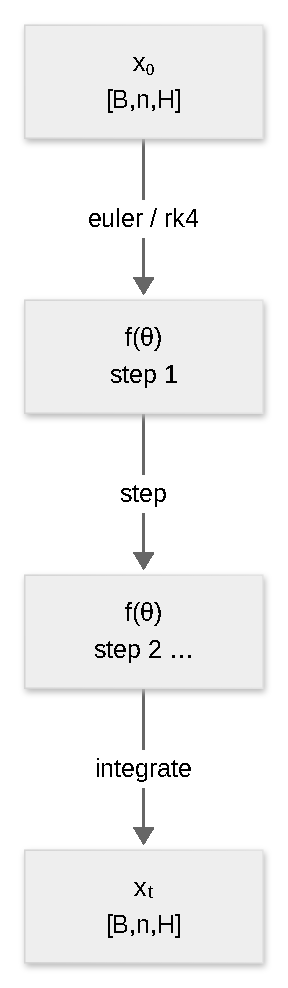
\includegraphics{figures/mixers/ode.pdf}}
\caption{Dataflow of the ODE transformer block: the hidden state is integrated through one or more Euler/RK4 steps before the output is read.}
\label{fig:mixer-ode}
\end{figure}
The ODE Transformer \citep{zhang_continuous_2021} interprets network depth as numerical integration of a continuous dynamical system, using higher-order Runge-Kutta solvers to reduce truncation error:

\begin{algorithmic}[1]
\State \textbf{Continuous formulation:} $\frac{dh(t)}{dt} = f_\theta(h(t), t)$ where $f_\theta$ is the transformer sub-network
\State \textbf{Runge-Kutta-4 discrete approximation:}
\State $k_1 \gets f_\theta(h_t, t)$
\State $k_2 \gets f_\theta(h_t + \tfrac{1}{2}k_1, t + \tfrac{1}{2}\Delta t)$
\State $k_3 \gets f_\theta(h_t + \tfrac{1}{2}k_2, t + \tfrac{1}{2}\Delta t)$
\State $k_4 \gets f_\theta(h_t + k_3, t + \Delta t)$
\State $h_{t+1} \gets h_t + \frac{\Delta t}{6}(k_1 + 2k_2 + 2k_3 + k_4)$ \Comment{weighted combination}
\end{algorithmic}

Instead of simple Euler residual connections $h_{t+1} = h_t + f_\theta(h_t)$, the RK4 block computes four intermediate evaluations and combines them with classical RK4 weights. To avoid vanishing gradients, the architecture introduces \textbf{learned gating} that interpolates between intermediate approximations:

\begin{algorithmic}[1]
\State $g \gets \sigma(\text{Linear}([k_1, k_2, k_3, k_4]))$ \Comment{learnable gate}
\State $h_{t+1} \gets h_t + g \cdot k_1 + (1-g) \cdot k_2$ \Comment{interpolated refinement}
\end{algorithmic}

This formulation reduces the effective number of parameters through weight sharing---the same $f_\theta$ is evaluated multiple times---while providing richer trajectory refinement.

\begin{itemize}[leftmargin=*]
    \item \textbf{Training complexity}: $\mathcal{O}(k \cdot n^2 \cdot d)$ where $k$ is the RK order (4 for RK4).
    \item \textbf{Inference complexity}: $\mathcal{O}(k \cdot n)$ per token (higher constant overhead).
    \item \textbf{Strengths}: Significantly higher accuracy on generation tasks (state-of-the-art BLEU); parameter-efficient via weight sharing.
    \item \textbf{Weaknesses}: High per-step compute; inference latency increases by constant factor $k$; complex gating required for stability.
\end{itemize}

\subsection{Test-Time Memory: Titans}

\begin{figure}[H]
\centering
\fitfigure{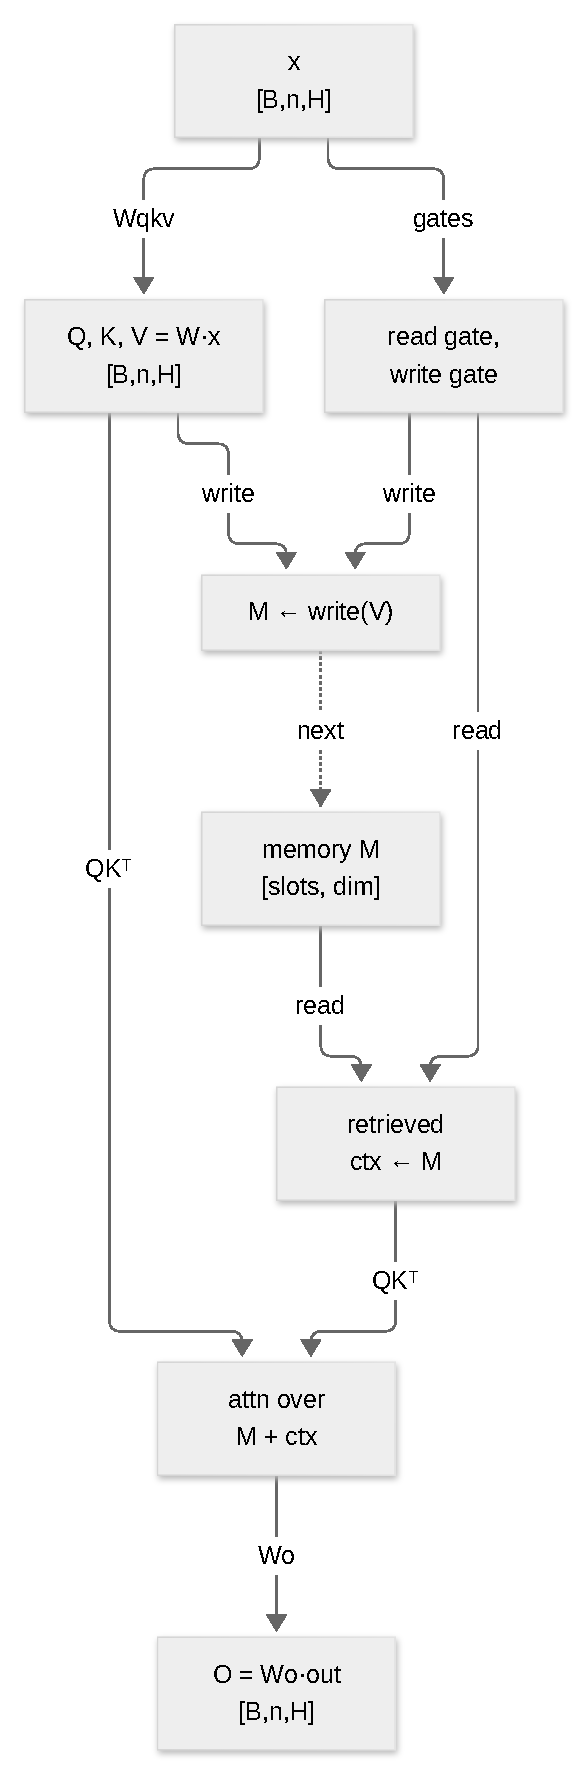
\includegraphics{figures/mixers/titan.pdf}}
\caption{Dataflow of Titans test-time memory: dense Q/K/V attention runs over a local window while read and write gates update an associative memory that carries across steps.}
\label{fig:mixer-titan}
\end{figure}

The Titans architecture \citep{behrouz_titans_2025} introduces an orthogonal dimension: instead of static weights, the model maintains a learnable memory that is \textit{updated during inference} based on a surprise-driven signal:

\begin{algorithmic}[1]
\State \textbf{Local short-term attention:} Apply standard or sparse attention within a fixed context window $c$
\State $y_t^{\text{local}} \gets \text{Attention}(q_t, k_{[t-c:t]}, v_{[t-c:t]})$
\State \textbf{Memory update signal (surprise):}
\State $S_t \gets \eta_t S_{t-1} - \theta_t \nabla_\ell(\mathcal{M}_{t-1}; x_t)$ \Comment{surprise as gradient of loss w.r.t. memory}
\State $\mathcal{M}_t \gets (1 - \alpha_t) \mathcal{M}_{t-1} + S_t$ \Comment{memory updated via EMA}
\State \textbf{Long-term memory retrieval:}
\State $y_t^{\text{memory}} \gets \mathcal{M}_t^* (q_t)$ \Comment{query memory module for retrieved information}
\State \textbf{Output combination:}
\State $y_t \gets y_t^{\text{local}} + \text{gate}(y_t^{\text{memory}})$ \Comment{combine local and retrieved memory}
\end{algorithmic}

The memory module $\mathcal{M}$ is literally updated during the forward pass by computing gradients of an associative loss and applying SGD steps with momentum. The decay rates $\eta_t, \theta_t, \alpha_t$ are themselves input-dependent, allowing the model to switch memory paradigms when context shifts.

\begin{itemize}[leftmargin=*]
    \item \textbf{Training complexity}: Roughly $\mathcal{O}(c^2 + n \cdot f)$ where $c$ is local window and $f$ is memory update overhead.
    \item \textbf{Inference complexity}: $\mathcal{O}(c^2)$ local attention plus $\mathcal{O}(1)$ memory retrieval per token.
    \item \textbf{Strengths}: Handles extreme context lengths; enables true associative recall; memory adapts to input.
    \item \textbf{Weaknesses}: Significantly more complex; inference includes gradient computation; higher coordination overhead.
\end{itemize}

\subsection{Pattern-Driven Mixer Dispatch}

The codebase selects a mixer per block from the configured \texttt{layer\_pattern}. The dispatch logic routes inference-time sparse blocks (\texttt{fasa\_attn}, \texttt{sparge\_attn}) to standard dense attention while the model is in training mode, and to their sparse implementation during evaluation; all other blocks route to the corresponding family implementation.

\begin{algorithm}[t]
\caption{Pattern-Driven Mixer Forward (Conceptual)}
\begin{algorithmic}[1]
\Require Hidden states $H$, pattern $P$, layer index $\ell$
\State $m \gets P[\ell \bmod |P|]$
\If{$m \in \{\texttt{fasa\_attn}, \texttt{sparge\_attn}\}$ and model is in training mode}
    \State $H \gets \text{softmax-attention}(H)$ \Comment{dense surrogate, same projections}
\ElsIf{$m=\texttt{standard\_attn}$}
    \State $H \gets \text{softmax-attention}(H)$
\ElsIf{$m=\texttt{sigmoid\_attn}$}
    \State $H \gets \text{sigmoid-attention}(H)$
\ElsIf{$m\in\{\texttt{retnet},\texttt{retnet\_attn}\}$}
    \State $H \gets \text{retention}(H)$
\ElsIf{$m=\texttt{mamba}$}
    \State $H \gets \text{selective-ssm}(H)$
\ElsIf{$m=\texttt{ode}$}
    \State $H \gets \text{rk-step}(H)$
\ElsIf{$m$ is a sparse attention key}
    \State $H \gets \text{sparse-attention-family}(H)$
\ElsIf{$m$ is a gated attention key}
    \State $H \gets \text{gated-attention-family}(H)$
\Else
    \State $H \gets \text{memory-augmented-attn}(H)$
\EndIf
\State \Return $H$
\end{algorithmic}
\end{algorithm}

The field exhibits a clear progression along two axes: (i) \textbf{computational efficiency}, moving from $O(n^2)$ to $O(n)$ or $O(1)$, and (ii) \textbf{memory adaptivity}, shifting from static weights to dynamic, test-time updated models. Standard attention remains the expressiveness baseline; Mamba and RetNet represent the practical efficiency frontier; Titans introduces an orthogonal innovation axis (test-time learning). The choice of architecture reflects the fundamental engineering constraint: expressiveness versus deployment cost. The latent-attention family, which compresses the KV cache into a low-rank latent, is covered in Appendix~\ref{sec:annex-latent}.
\section{Latent and Low-Rank Attention Families}
\label{sec:annex-latent}

This annex covers the latent / low-rank KV compression family of attention mechanisms. These architectures compress the per-token key--value state into a low-rank latent vector that is the only quantity materialised in the KV cache during decoding, then reconstruct full multi-head keys and values on the fly. The family unifies grouped-query, latent, factorised, and temporal-latent designs under a common low-rank bottleneck.

\subsection{Multi-Head Latent Attention (MLA)}

\begin{figure}[H]
\centering
\fitfigure{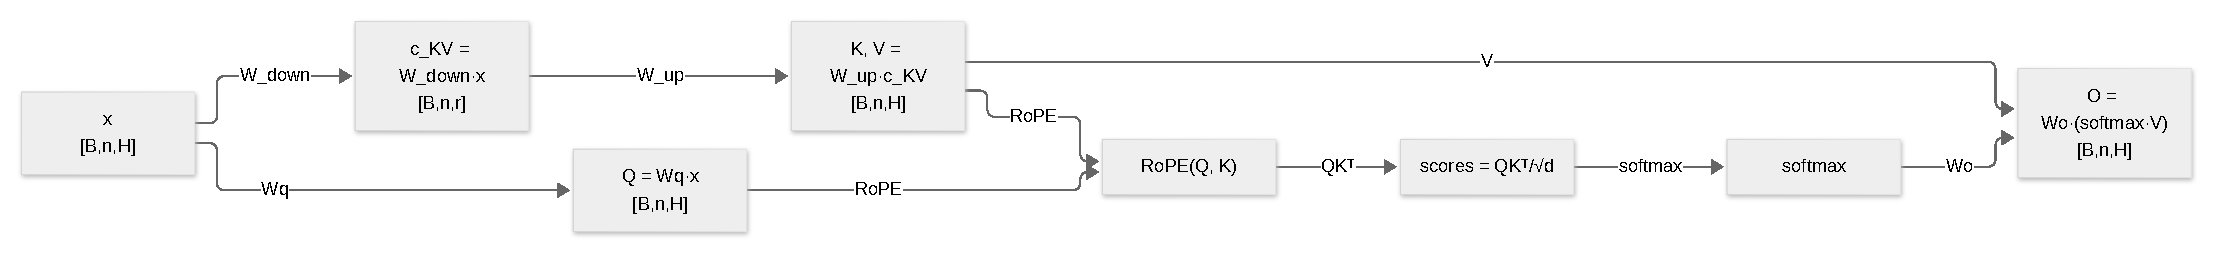
\includegraphics{figures/mixers/mla.pdf}}
\caption{Dataflow of multi-head latent attention: keys and values are down-projected to a low-rank latent, up-projected back, and attended with the query after RoPE.}
\label{fig:mixer-mla}
\end{figure}
Multi-Head Latent Attention (MLA) \citep{mehta_mla_2025} compresses the per-token key--value state into a single low-rank latent vector $c_{KV}$ of rank $r_{kv}$, which is the only quantity materialised in the KV cache during decoding. A pair of up-projection matrices reconstructs the full multi-head keys and values on the fly, while RoPE is applied to the decompressed query and key tensors so that positional structure is preserved. The authors show that the Pareto-optimal latent width sits near $r_{kv} = d_{\text{hidden}} / 2$, at which point MLA halves the KV cache yet matches multi-head attention (MHA) quality on small models.

\subsubsection{Mathematical Formulation}
\[
c_{KV} = W_{DKV}\, x \in \mathbb{R}^{r_{kv}}, \qquad
k = W_{UK}\, c_{KV}, \qquad
v = W_{UV}\, c_{KV}, \qquad
q = W_{Q}\, x.
\]
\[
\tilde q = \text{RoPE}(q), \quad \tilde k = \text{RoPE}(k), \qquad
\text{attn} = \texttt{softmax}\!\left(\frac{\tilde q\, \tilde k^\top}{\sqrt{d_h}}\right) v.
\]

\subsubsection{Algorithmic Pseudocode}
\begin{algorithmic}[1]
\State \textbf{Input:} hidden state $x \in \mathbb{R}^{n \times d}$, rank $r_{kv}$, projections $W_{DKV}, W_{UK}, W_{UV}, W_{Q}$
\State $c_{KV} \gets W_{DKV}\, x$ \Comment{down-project to latent of rank $r_{kv}$ (cached at inference)}
\State $k \gets W_{UK}\, c_{KV}$, \quad $v \gets W_{UV}\, c_{KV}$ \Comment{up-project to full heads}
\State $q \gets W_{Q}\, x$
\State $\tilde q \gets \text{RoPE}(q)$, \quad $\tilde k \gets \text{RoPE}(k)$ \Comment{apply rotary embeddings}
\State $\text{weights} \gets \texttt{softmax}(\tilde q\, \tilde k^\top / \sqrt{d_h})$
\State \textbf{Output:} $\mathbf{Y} = \text{weights} \cdot v$
\end{algorithmic}

\subsubsection{Key Characteristics}
\begin{itemize}[leftmargin=*]
    \item \textbf{Training complexity}: $\mathcal{O}(n^2 \cdot d)$ (full attention on decompressed heads).
    \item \textbf{Inference complexity}: $\mathcal{O}(n)$ per token, $\mathcal{O}(r_{kv} \cdot n)$ KV-cache space (latent only).
    \item \textbf{Trainable}: fully trainable; $r_{kv}$ is a hyperparameter (Pareto-optimal $\approx d/2$).
    \item \textbf{Strengths}: Halves KV cache versus MHA at matched quality; RoPE-compatible; clean latent bottleneck.
    \item \textbf{Limitations}: Up-projection adds decode FLOPs; latent rank is a fixed global budget shared across heads.
\end{itemize}

\subsection{Group-Query Latent Attention (GQLA)}

\begin{figure}[H]
\centering
\fitfigure{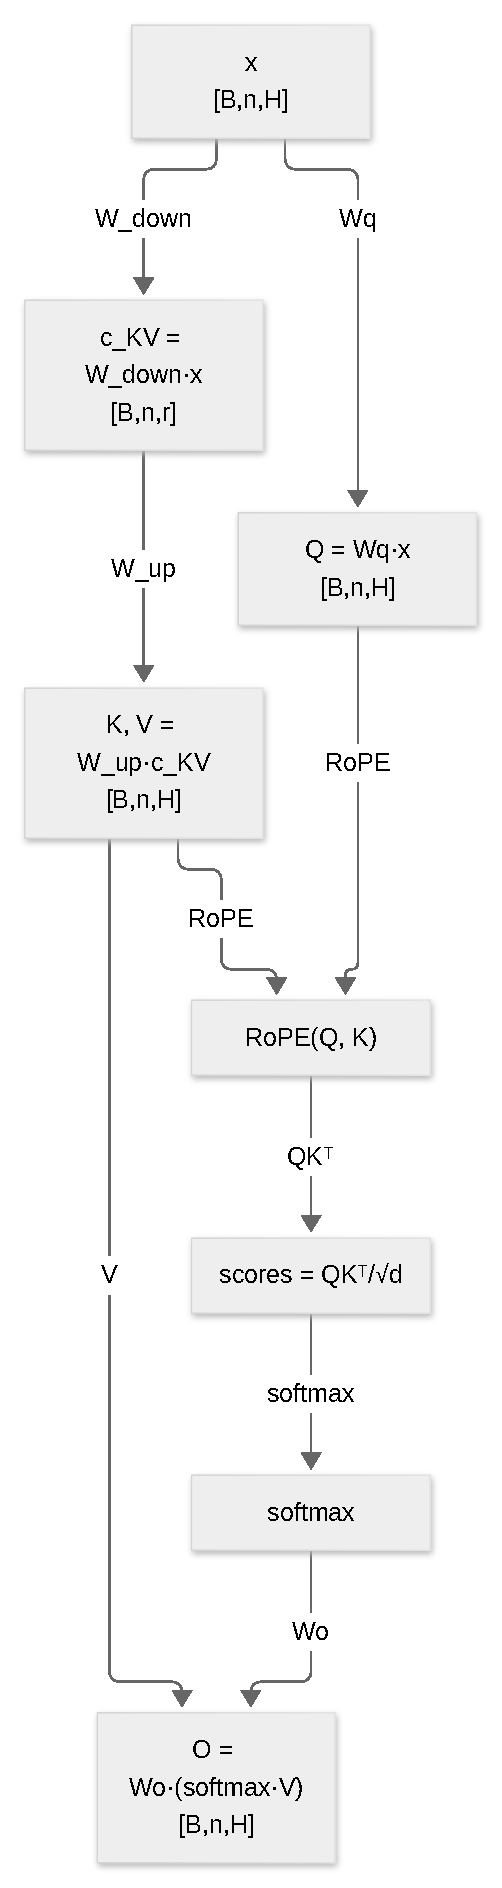
\includegraphics{figures/mixers/gqla.pdf}}
\caption{Dataflow of group-query latent attention: the shared latent cache is up-projected to key/value heads and combined with grouped queries.}
\label{fig:mixer-gqla}
\end{figure}
Group-Query Latent Attention (GQLA) \citep{meng_gqla_2026} is a minimal modification of MLA that exposes two algebraically equivalent decoding paths over the same trained weights: an MQA-absorb path (fusing the up-projection into the query, optimal on H100-class hardware) and a GQA-expanded path (materialising full keys/values, optimal on H20 / multi-token-prediction hardware). The two paths are mathematically identical because the up-projection is linear, so $\texttt{softmax}(q_{\text{absorbed}} \cdot c_{KV}^\top) = \texttt{softmax}((q \cdot W_{UK}^\top) \cdot c_{KV}^\top)$, allowing hardware-adaptive dispatch with no retraining.

\subsubsection{Mathematical Formulation}
Same latent as MLA:
\[
c_{KV} = W_{DKV}\, x, \qquad k = W_{UK}\, c_{KV}, \qquad v = W_{UV}\, c_{KV}, \qquad q = W_{Q}\, x.
\]
\[
\text{Path A (MQA-absorb): } \text{attn} = \texttt{softmax}\!\left(\frac{(q\, W_{UK}^\top)\, c_{KV}^\top}{\sqrt{d_h}}\right) (W_{UV}\, c_{KV}).
\]
\[
\text{Path B (GQA-expanded): } \text{attn} = \texttt{softmax}\!\left(\frac{q\, k^\top}{\sqrt{d_h}}\right) v, \quad k = W_{UK} c_{KV},\ v = W_{UV} c_{KV}.
\]

\subsubsection{Algorithmic Pseudocode}
\begin{algorithmic}[1]
\State \textbf{Input:} $x$, weights $W_{DKV}, W_{UK}, W_{UV}, W_{Q}$, hardware flag $\text{hw} \in \{\text{H100}, \text{H20}\}$
\State $c_{KV} \gets W_{DKV}\, x$ \Comment{shared latent, cached}
\State $q \gets W_{Q}\, x$
\If{$\text{hw} == \text{H100}$} \Comment{MQA-absorb path}
    \State $q_{\text{abs}} \gets q\, W_{UK}^\top$ \Comment{absorb up-projection into query}
    \State $\text{weights} \gets \texttt{softmax}(q_{\text{abs}}\, c_{KV}^\top / \sqrt{d_h})$
    \State $\mathbf{Y} \gets \text{weights} \cdot (W_{UV}\, c_{KV})$
\Else \Comment{GQA-expanded path}
    \State $k \gets W_{UK}\, c_{KV}$, \quad $v \gets W_{UV}\, c_{KV}$
    \State $\text{weights} \gets \texttt{softmax}(q\, k^\top / \sqrt{d_h})$
    \State $\mathbf{Y} \gets \text{weights} \cdot v$
\EndIf
\State \textbf{Output:} $\mathbf{Y}$
\end{algorithmic}

\subsubsection{Key Characteristics}
\begin{itemize}[leftmargin=*]
    \item \textbf{Training complexity}: $\mathcal{O}(n^2 \cdot d)$, identical to MLA.
    \item \textbf{Inference complexity}: $\mathcal{O}(n)$ per token, $\mathcal{O}(r_{kv} \cdot n)$ latent state; path chosen by hardware.
    \item \textbf{Trainable}: trained once; the two decoding paths reuse the same weights.
    \item \textbf{Strengths}: Hardware-adaptive decode with no quality loss; algebraic equivalence guarantees consistency.
    \item \textbf{Limitations}: Same latent-rank tradeoffs as MLA; path selection is a deployment-time heuristic.
\end{itemize}

\subsection{Multi-Head Low-Rank Attention (MLRA)}

\begin{figure}[H]
\centering
\fitfigure{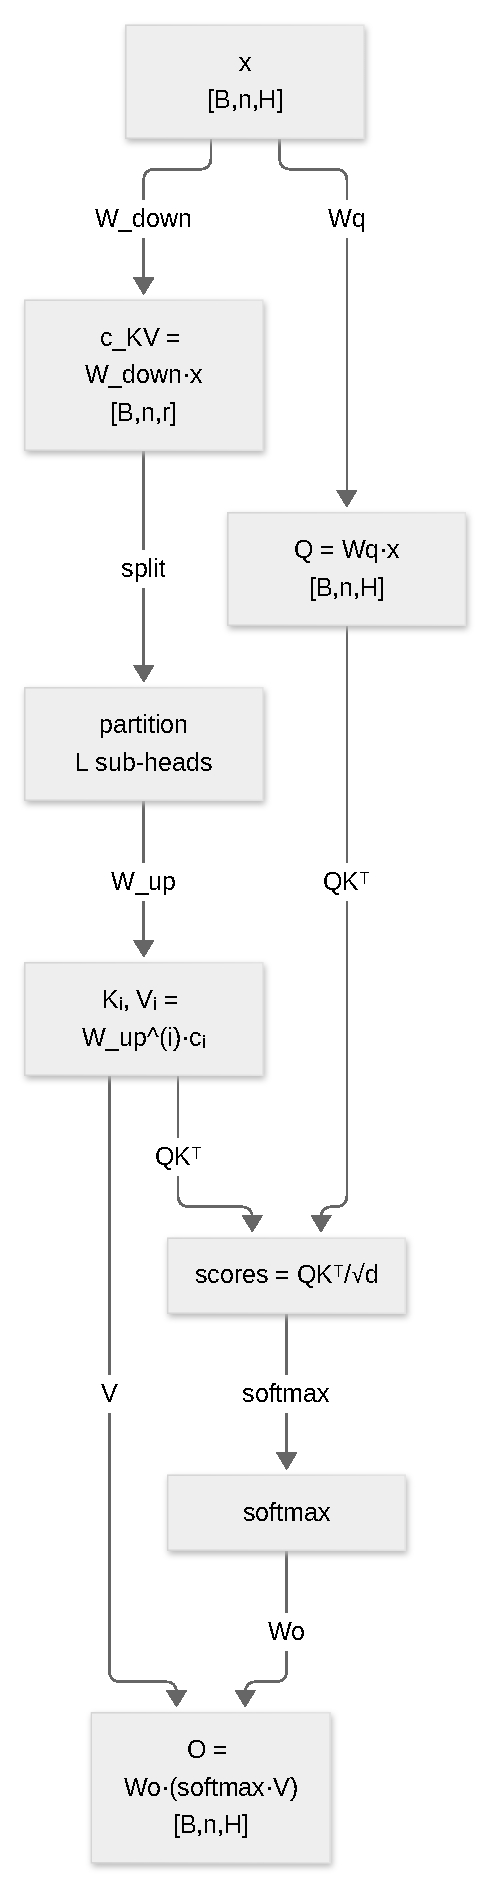
\includegraphics{figures/mixers/mlra.pdf}}
\caption{Dataflow of multi-head low-rank attention: the latent is partitioned across sub-heads, each with its own up-projection, before attention.}
\label{fig:mixer-mlra}
\end{figure}
Multi-Head Low-Rank Attention (MLRA) \citep{liu_mlra_2026} refactors the single MLA latent into $L$ disjoint sub-heads each of rank $r/L$, so that the KV cache can be partitioned across $L$ devices for 4-way tensor-parallel decoding (each device loads only $1/L$ of the cache). Per-sub-head up-projections reconstruct the corresponding slice of the full heads and are concatenated, yielding a 2.8$\times$ decode speedup over MLA while preserving the global latent budget.

\subsubsection{Mathematical Formulation}
\[
c_{KV} = [c_1, c_2, \ldots, c_L], \quad c_i \in \mathbb{R}^{r/L}, \qquad c_{KV} = W_{DKV}\, x.
\]
\[
k_i = W_{UK}^{(i)}\, c_i, \quad v_i = W_{UV}^{(i)}\, c_i, \qquad
k = [k_1; \ldots; k_L], \quad v = [v_1; \ldots; v_L].
\]
\[
\text{attn} = \texttt{softmax}\!\left(\frac{q\, k^\top}{\sqrt{d_h}}\right) v.
\]

\subsubsection{Algorithmic Pseudocode}
\begin{algorithmic}[1]
\State \textbf{Input:} $x$, sub-head count $L$, per-sub-head projections $W_{UK}^{(i)}, W_{UV}^{(i)}$
\State $c_{KV} \gets W_{DKV}\, x = [c_1, \ldots, c_L]$ \Comment{partition latent into $L$ blocks}
\For{$i = 1, \ldots, L$ (parallel across $L$ devices)}
    \State $k_i \gets W_{UK}^{(i)}\, c_i$, \quad $v_i \gets W_{UV}^{(i)}\, c_i$
\EndFor
\State $k \gets \texttt{concat}(k_1, \ldots, k_L)$, \quad $v \gets \texttt{concat}(v_1, \ldots, v_L)$
\State $\text{weights} \gets \texttt{softmax}(q\, k^\top / \sqrt{d_h})$
\State \textbf{Output:} $\mathbf{Y} = \text{weights} \cdot v$
\end{algorithmic}

\subsubsection{Key Characteristics}
\begin{itemize}[leftmargin=*]
    \item \textbf{Training complexity}: $\mathcal{O}(n^2 \cdot d)$ (full attention on concatenated heads).
    \item \textbf{Inference complexity}: $\mathcal{O}(n)$ per token, $\mathcal{O}(r_{kv} \cdot n)$ state partitioned across $L$ devices.
    \item \textbf{Trainable}: fully trainable; $L$ controls partition granularity.
    \item \textbf{Strengths}: 2.8$\times$ decode speedup; clean 4-way tensor-parallel cache sharding; preserves total latent budget.
    \item \textbf{Limitations}: Requires $L$ to divide $r_{kv}$; more projection matrices than MLA; inter-device all-reduce on output.
\end{itemize}

\subsection{Tucker Attention}

\begin{figure}[H]
\centering
\fitfigure{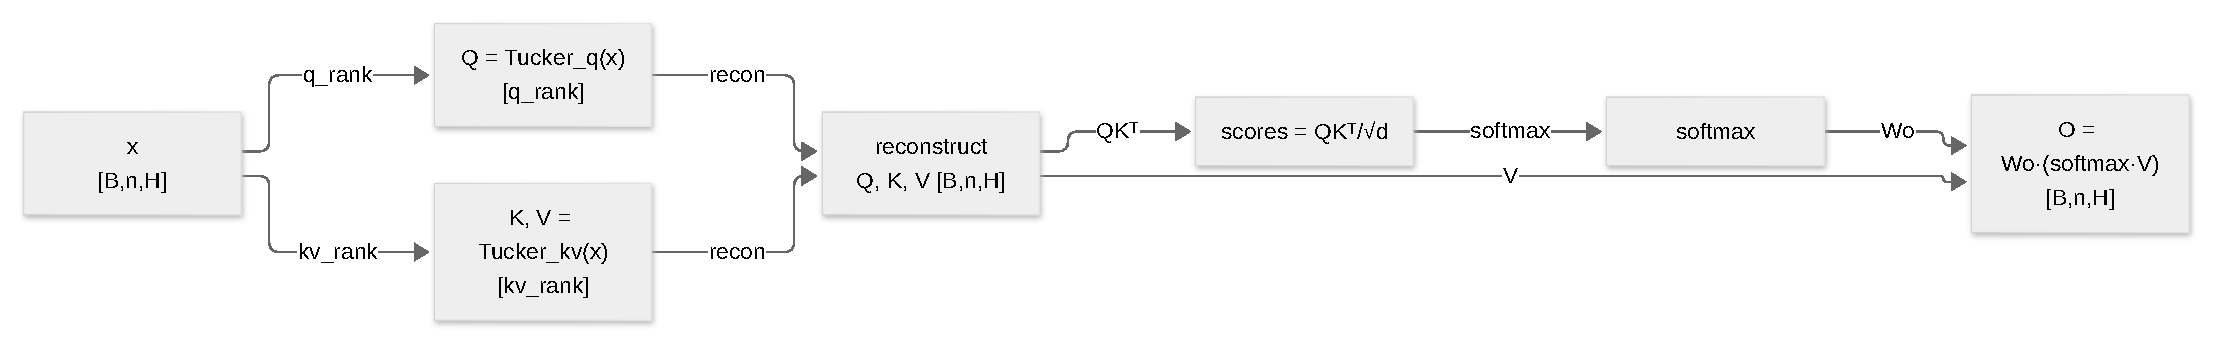
\includegraphics{figures/mixers/tucker.pdf}}
\caption{Dataflow of Tucker attention: queries and key/values are projected through Tucker factors and reconstructed before the scaled dot product.}
\label{fig:mixer-tucker}
\end{figure}
Tucker Attention \citep{klein_tucker_2026} unifies MHA, GQA and MLA under a single Tucker-style factorisation of the query/key/value weight tensors with independent ranks $q_{\text{rank}}, k_{\text{rank}}, v_{\text{rank}}$. MHA is recovered when all ranks equal the hidden size, GQA when $k_{\text{rank}} = v_{\text{rank}} < d$, and MLA when $k_{\text{rank}} = v_{\text{rank}}$ equals the latent rank. Because the factorisation is a pure linear reparameterisation, the method is fully compatible with FlashAttention and RoPE, and yields an order of magnitude fewer parameters for comparable metrics.

\subsubsection{Mathematical Formulation}
\[
\mathbf{Q} = W_{Q,\text{core}}\, W_{Q,\text{factor}}\, x, \qquad
\mathbf{K} = W_{K,\text{core}}\, W_{K,\text{factor}}\, x, \qquad
\mathbf{V} = W_{V,\text{core}}\, W_{V,\text{factor}}\, x.
\]
\[
\text{attn} = \texttt{softmax}\!\left(\frac{\mathbf{Q}\, \mathbf{K}^\top}{\sqrt{d_h}}\right) \mathbf{V}.
\]
Special cases: MHA $\Leftrightarrow q_{\text{rank}} = k_{\text{rank}} = v_{\text{rank}} = d$; GQA $\Leftrightarrow k_{\text{rank}} = v_{\text{rank}} < d$; MLA $\Leftrightarrow k_{\text{rank}} = v_{\text{rank}} = r_{kv}$.

\subsubsection{Algorithmic Pseudocode}
\begin{algorithmic}[1]
\State \textbf{Input:} $x$, ranks $q_{\text{rank}}, k_{\text{rank}}, v_{\text{rank}}$, core/factor matrices
\State $\mathbf{Q} \gets W_{Q,\text{core}}\, W_{Q,\text{factor}}\, x$ \Comment{rank-$q_{\text{rank}}$ factorised query}
\State $\mathbf{K} \gets W_{K,\text{core}}\, W_{K,\text{factor}}\, x$ \Comment{rank-$k_{\text{rank}}$ factorised key}
\State $\mathbf{V} \gets W_{V,\text{core}}\, W_{V,\text{factor}}\, x$ \Comment{rank-$v_{\text{rank}}$ factorised value}
\State \textbf{Apply RoPE to $\mathbf{Q}, \mathbf{K}$ if positional encoding is used}
\State $\text{weights} \gets \texttt{softmax}(\mathbf{Q}\, \mathbf{K}^\top / \sqrt{d_h})$ \Comment{FlashAttention-compatible}
\State \textbf{Output:} $\mathbf{Y} = \text{weights} \cdot \mathbf{V}$
\end{algorithmic}

\subsubsection{Key Characteristics}
\begin{itemize}[leftmargin=*]
    \item \textbf{Training complexity}: $\mathcal{O}(n^2 \cdot d)$ on the reconstructed tensors.
    \item \textbf{Inference complexity}: $\mathcal{O}(n)$ per token; cache size governed by $k_{\text{rank}}$.
    \item \textbf{Trainable}: ranks are hyperparameters; the factorisation is a drop-in weight reparameterisation.
    \item \textbf{Strengths}: Unifies MHA/GQA/MLA; order-of-magnitude parameter reduction at matched metrics; FlashAttention/RoPE compatible.
    \item \textbf{Limitations}: Two matmuls per projection add latency; rank selection is a per-task tuning problem.
\end{itemize}

\subsection{Interleaved Head Attention (IHA)}

\begin{figure}[H]
\centering
\fitfigure{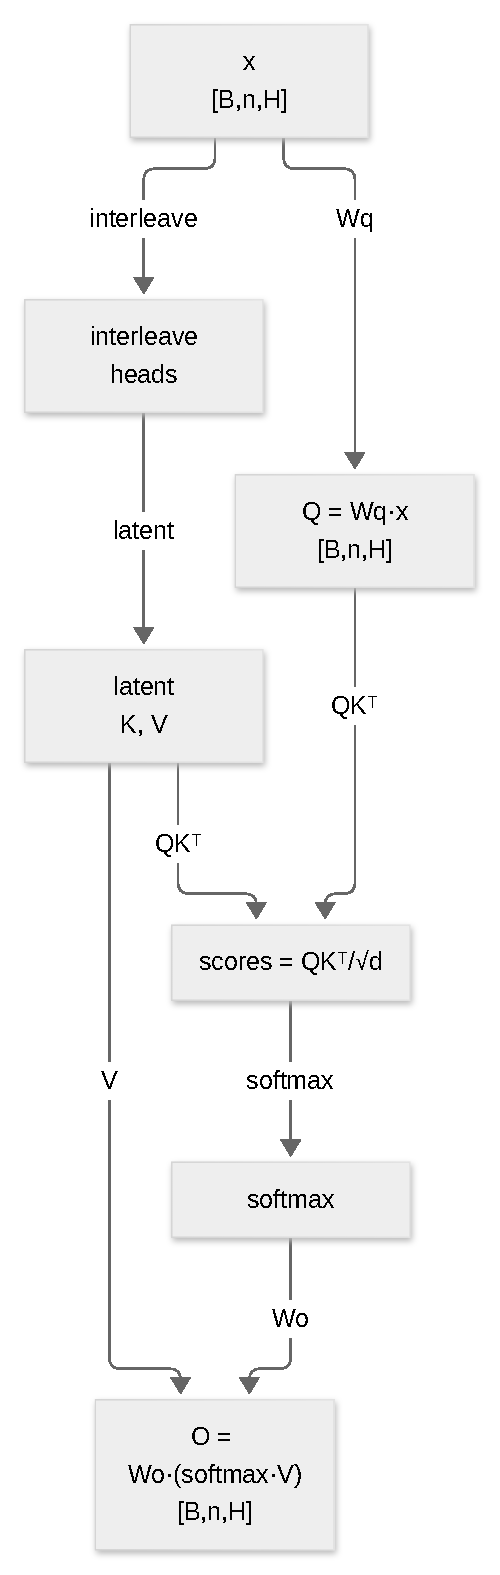
\includegraphics{figures/mixers/iha.pdf}}
\caption{Dataflow of interleaved-head attention: heads are interleaved into a latent key/value representation that is attended by the query.}
\label{fig:mixer-iha}
\end{figure}
Interleaved Head Attention (IHA) \citep{duvvuri_iha_2026} constructs $P$ pseudo-heads per original head (typically $P = H$) where each pseudo query/key/value is a learned linear combination of all $H$ original heads. This induces up to $P^2$ distinct attention patterns per head at an $\mathcal{O}(H^2 P)$ overhead. Theoretically, IHA needs only $\Theta(\sqrt{k}\, n^2)$ parameters versus $\Theta(k\, n^2)$ for MHA on the Polynomial task; empirically it delivers $+10$--$20\%$ on RULER multi-key retrieval, $+5.8\%$ on GSM8K and $+2.8\%$ on MATH-500.

\subsubsection{Mathematical Formulation}
\[
q_{\text{pseudo}}[p] = \sum_{h=1}^{H} \text{mix}_q[p, h]\, q[h], \quad
k_{\text{pseudo}}[p] = \sum_{h} \text{mix}_k[p, h]\, k[h], \quad
v_{\text{pseudo}}[p] = \sum_{h} \text{mix}_v[p, h]\, v[h].
\]
\[
\text{attn}_p = \texttt{softmax}\!\left(\frac{q_{\text{pseudo}}[p]\, k_{\text{pseudo}}[p]^\top}{\sqrt{d_h}}\right) v_{\text{pseudo}}[p],
\qquad
\mathbf{Y}[h] = \frac{1}{P} \sum_{p} \text{attn}_p[h].
\]

\subsubsection{Algorithmic Pseudocode}
\begin{algorithmic}[1]
\State \textbf{Input:} per-head $q[h], k[h], v[h]$, mixing matrices $\text{mix}_q, \text{mix}_k, \text{mix}_v \in \mathbb{R}^{P \times H}$
\For{$p = 1, \ldots, P$}
    \State $q_p \gets \sum_h \text{mix}_q[p,h]\, q[h]$ \Comment{learned mix across heads}
    \State $k_p \gets \sum_h \text{mix}_k[p,h]\, k[h]$, \quad $v_p \gets \sum_h \text{mix}_v[p,h]\, v[h]$
    \State $\text{attn}_p \gets \texttt{softmax}(q_p\, k_p^\top / \sqrt{d_h})\, v_p$
\EndFor
\State \textbf{Output:} $\mathbf{Y}[h] \gets \frac{1}{P} \sum_p \text{attn}_p[h]$ \Comment{average pseudo-head outputs per head}
\end{algorithmic}

\subsubsection{Key Characteristics}
\begin{itemize}[leftmargin=*]
    \item \textbf{Training complexity}: $\mathcal{O}(n^2 \cdot H \cdot P)$ with $P \approx H$, i.e.\ $\mathcal{O}(n^2 \cdot H^2)$.
    \item \textbf{Inference complexity}: $\mathcal{O}(n)$ per token with KV cache; extra $\mathcal{O}(H^2 P)$ mixing overhead.
    \item \textbf{Trainable}: mixing matrices are learned; $P$ is a hyperparameter.
    \item \textbf{Strengths}: $\Theta(\sqrt{k})$ parameter efficiency on Polynomial; large gains on retrieval and reasoning benchmarks.
    \item \textbf{Limitations}: Quadratic-in-heads mixing cost; more attention patterns to compute; added latency at large $H$.
\end{itemize}

\subsection{Grouped-head laTenT Attention (GTA)}

\begin{figure}[H]
\centering
\fitfigure{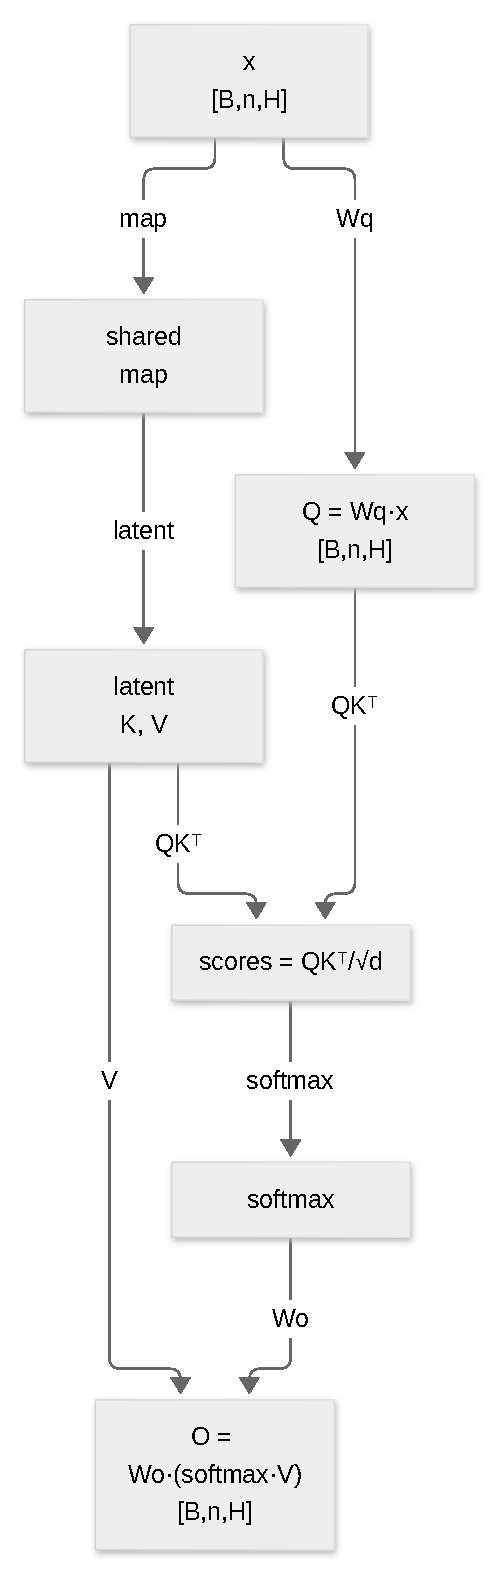
\includegraphics{figures/mixers/gta.pdf}}
\caption{Dataflow of grouped-head latent attention: a shared map produces the latent key/value state consumed by the grouped heads.}
\label{fig:mixer-gta}
\end{figure}
Grouped-head laTenT Attention (GTA) \citep{sun_gta_2025} combines two compressions: (1) a \emph{shared attention map} --- one attention-score tensor per group of heads, reused across all heads in the group, shrinking the key cache; and (2) a \emph{nonlinear value decoder} --- the value cache is compressed to a latent by a down-projection and reconstructed by a SiLU-gated up-projection before the output projection. GTA cuts attention FLOPs by up to 62.5\% versus GQA, shrinks the KV cache by up to 70\%, and yields a 2$\times$ end-to-end inference speedup.

\subsubsection{Mathematical Formulation}
\[
q_g = \texttt{mean}(q[\text{group } g]), \quad k_g = \texttt{mean}(k[\text{group } g]), \quad
\text{attn}_g = \texttt{softmax}\!\left(\frac{q_g\, k_g^\top}{\sqrt{d_h}}\right) \text{ (reused across the group)}.
\]
\[
v_{\text{latent}} = W_{DV}\, x, \qquad v = \text{SiLU}(W_{UV}\, v_{\text{latent}}), \qquad
\mathbf{Y} = \text{attn}_g \cdot v.
\]

\subsubsection{Algorithmic Pseudocode}
\begin{algorithmic}[1]
\State \textbf{Input:} $q, k$ per head, hidden $x$, group partition $\{g\}$
\State $v_{\text{latent}} \gets W_{DV}\, x$ \Comment{compress values to latent (cached)}
\State $v \gets \text{SiLU}(W_{UV}\, v_{\text{latent}})$ \Comment{nonlinear value decode}
\For{each group $g$}
    \State $q_g \gets \texttt{mean}(q[g])$, \quad $k_g \gets \texttt{mean}(k[g])$ \Comment{shared per-group queries/keys}
    \State $\text{attn}_g \gets \texttt{softmax}(q_g\, k_g^\top / \sqrt{d_h})$
    \State $\mathbf{Y}[g] \gets \text{attn}_g \cdot v[g]$ \Comment{one map reused for all heads in $g$}
\EndFor
\State \textbf{Output:} $\mathbf{Y}$
\end{algorithmic}

\subsubsection{Key Characteristics}
\begin{itemize}[leftmargin=*]
    \item \textbf{Training complexity}: $\mathcal{O}(n^2 \cdot G \cdot d_h)$ where $G$ is the number of groups (vs $H$ heads for GQA).
    \item \textbf{Inference complexity}: $\mathcal{O}(n)$ per token; value cache $\mathcal{O}(r_v \cdot n)$, key cache reduced by group sharing.
    \item \textbf{Trainable}: group assignment and latent rank are trainable/hyperparameters.
    \item \textbf{Strengths}: up to 62.5\% attention-FLOP reduction, 70\% KV-cache shrink, 2$\times$ end-to-end speedup.
    \item \textbf{Limitations}: Shared map reduces per-head diversity; nonlinear decoder adds latency; grouping must be chosen carefully.
\end{itemize}

\subsection{Multi-head Temporal Latent Attention (MTLA)}

\begin{figure}[H]
\centering
\fitfigure{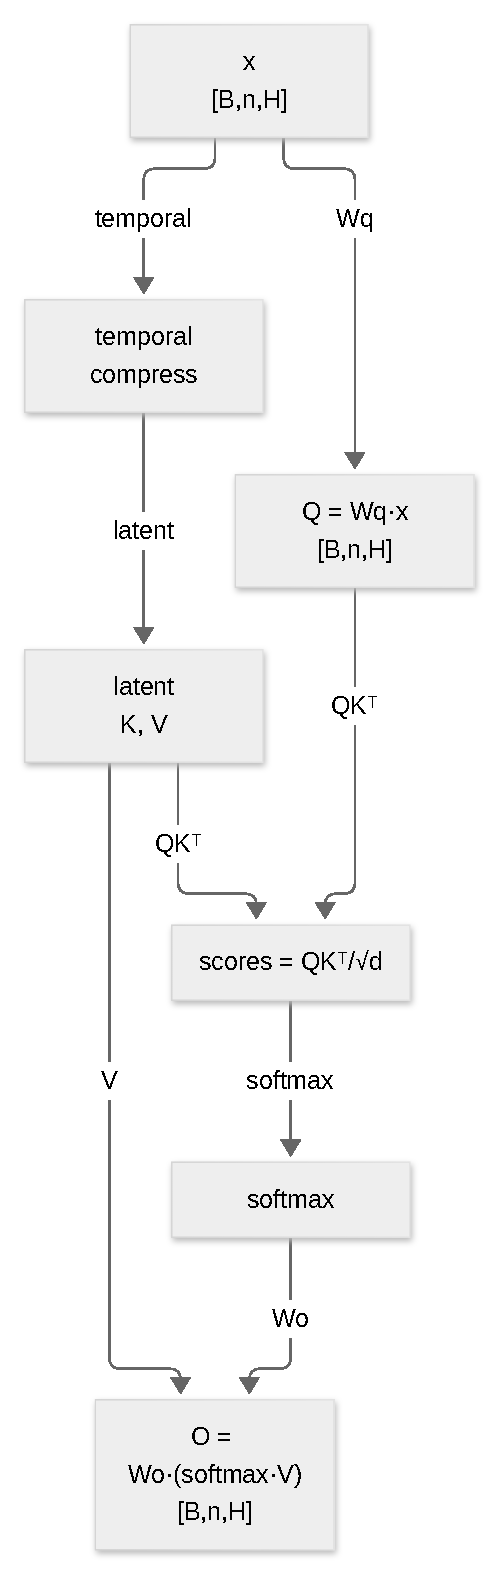
\includegraphics{figures/mixers/mtla.pdf}}
\caption{Dataflow of multi-head temporal latent attention: a temporal compression stage produces the latent key/value state attended by the query.}
\label{fig:mixer-mtla}
\end{figure}
Multi-head Temporal Latent Attention (MTLA) \citep{deng_mtla_2025} extends MLA along the temporal axis: a hyper-network dynamically merges $m$ temporally adjacent KV-cache vectors into a single slot, shrinking the temporal length by a factor of $m$. A stride-aware causal mask keeps parallel training consistent with autoregressive inference, yielding a 5.3$\times$ decode speedup and 8.3$\times$ GPU-memory reduction versus MHA on En--De speech translation.

\subsubsection{Mathematical Formulation}
\[
c_{KV}^{(t)} = W_{DKV}\, x^{(t)} \in \mathbb{R}^{r_{kv}} \text{ (per-token latent)}.
\]
\[
\bar c_{KV}^{(j)} = \sum_{i=0}^{m-1} \alpha_i\, c_{KV}^{(s j + i)}, \qquad \alpha_i = \texttt{sigmoid}(\text{HyperNet}(c_{KV}^{(s j + i)})),
\]
where $s$ is the stride and $m$ the merge window. Queries attend over merged slots $\bar c_{KV}$ with a stride-aware causal mask $M_{\text{stride}}$:
\[
\text{attn} = \texttt{softmax}\!\left(\frac{q\, \bar k^\top}{\sqrt{d_h}} + M_{\text{stride}}\right) \bar v, \quad \bar k = W_{UK}\, \bar c_{KV},\ \bar v = W_{UV}\, \bar c_{KV}.
\]

\subsubsection{Algorithmic Pseudocode}
\begin{algorithmic}[1]
\State \textbf{Input:} per-token latents $c_{KV}^{(t)}$, merge window $m$, stride $s$
\State \textbf{Merge phase (hyper-network):}
\For{each merged slot $j = 0, 1, \ldots$}
    \State $\alpha_i \gets \texttt{sigmoid}(\text{HyperNet}(c_{KV}^{(s j + i)}))$ for $i = 0, \ldots, m-1$
    \State $\bar c_{KV}^{(j)} \gets \sum_{i=0}^{m-1} \alpha_i\, c_{KV}^{(s j + i)}$ \Comment{gated average over window}
\EndFor
\State $\bar k \gets W_{UK}\, \bar c_{KV}$, \quad $\bar v \gets W_{UV}\, \bar c_{KV}$
\State $\text{weights} \gets \texttt{softmax}(q\, \bar k^\top / \sqrt{d_h} + M_{\text{stride}})$ \Comment{stride-aware causal mask}
\State \textbf{Output:} $\mathbf{Y} = \text{weights} \cdot \bar v$
\end{algorithmic}

\subsubsection{Key Characteristics}
\begin{itemize}[leftmargin=*]
    \item \textbf{Training complexity}: $\mathcal{O}(n^2 \cdot d / m)$ on the merged sequence (length $\lceil n/m \rceil$) plus hyper-network cost.
    \item \textbf{Inference complexity}: $\mathcal{O}(n/m)$ per token over merged slots; $\mathcal{O}(r_{kv} \cdot n / m)$ state.
    \item \textbf{Trainable}: hyper-network and merge window $m$ are learned/chosen; stride-aware mask enforces consistency.
    \item \textbf{Strengths}: 5.3$\times$ decode speedup, 8.3$\times$ GPU-memory reduction vs MHA; temporal compression orthogonal to rank compression.
    \item \textbf{Limitations}: Merge window can blur fine temporal detail; hyper-network adds compute; mask design is non-trivial.
\end{itemize}

\subsection{Architectural Comparison and Synthesis}

\subsection{Compressed Convolutional Attention (CCA)}

\begin{figure}[H]
\centering
\fitfigure{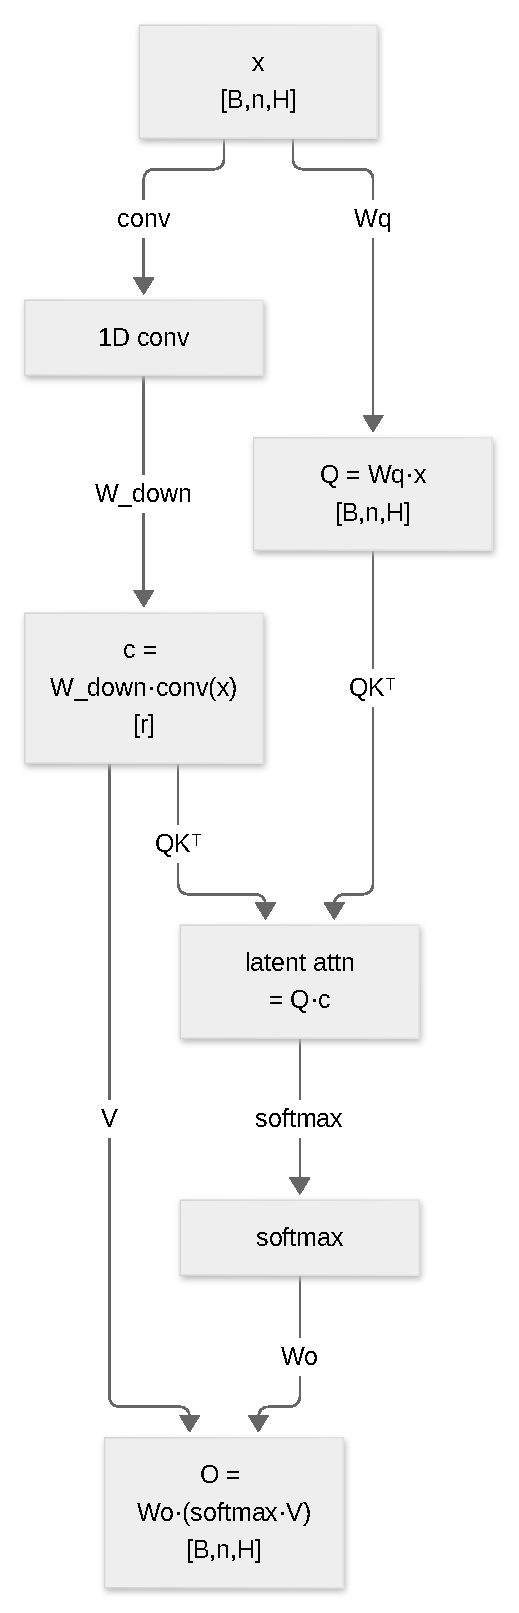
\includegraphics{figures/mixers/cca.pdf}}
\caption{Dataflow of compressed convolutional attention: a 1D convolution feeds a latent compression $c$, which the query attends directly.}
\label{fig:mixer-cca}
\end{figure}
Compressed Convolutional Attention (CCA) \citep{figliola_cca_2025} takes a fundamentally different approach to latent attention: rather than compressing the KV-cache and then up-projecting to full width before attending (as MLA/GQLA/MLRA do), CCA down-projects queries, keys, and values into a shared latent and performs the \emph{entire} attention operation inside it. There are no Q/K/V up-projection matrices---only a single output up-projection $\tilde{W}_O$ maps the latent output back to the residual stream. This simultaneously reduces parameters, KV-cache size, \textbf{and} attention FLOPs by the compression factor $C = E/\tilde{e}$, whereas MLA only shrinks the cache.

To make attention in the fully compressed latent viable, CCA introduces three innovations: (1) two causal convolutions on the packed q/k tensor (a depth-wise sequence convolution and a head-wise grouped channel convolution), (2) q-k-mean (adds the pre-convolution mean of q and k to the post-convolution values), and (3) value-shift (each head receives half its values from the current token and half from the previous token via two independent projections). After these steps, QK L2-normalisation and a learnable key temperature $\beta$ are applied, RoPE is applied \emph{directly in the latent} (no separate RoPE head needed), and standard softmax attention is computed.

\subsubsection{Mathematical Formulation}
\[
\tilde{q}_{\text{pre}} = \tilde{W}_Q\, x, \qquad \tilde{k}_{\text{pre}} = \tilde{W}_K\, x, \qquad \tilde{e} = E / C.
\]
\[
\tilde{q} = \text{Conv}(\tilde{q}_{\text{pre}}) + \tfrac{1}{2}(\tilde{q}_{\text{pre}} + \tilde{k}_{\text{pre}}), \qquad
\tilde{k} = \text{Conv}(\tilde{k}_{\text{pre}}) + \tfrac{1}{2}(\tilde{q}_{\text{pre}} + \tilde{k}_{\text{pre}}).
\]
\[
\tilde{v} = [\tilde{W}_{V_1}\, x_t \;\|\; \tilde{W}_{V_2}\, x_{t-1}], \qquad
\hat{q} = \frac{\tilde{q} \sqrt{d_h}}{\|\tilde{q}\|}, \quad \hat{k} = \frac{\tilde{k} \sqrt{d_h}}{\|\tilde{k}\|} e^{\beta}.
\]
\[
\text{attn} = \texttt{softmax}\!\left(\frac{\text{RoPE}(\hat{q})\, \text{RoPE}(\hat{k})^\top}{\sqrt{d_h}}\right) \tilde{v}, \qquad
\mathbf{Y} = \tilde{W}_O\, \text{attn}.
\]

\subsubsection{Algorithmic Pseudocode}
\begin{algorithmic}[1]
\State \textbf{Input:} hidden state $x \in \mathbb{R}^{n \times E}$, compression factor $C$, projections $\tilde{W}_Q, \tilde{W}_K, \tilde{W}_{V_1}, \tilde{W}_{V_2}, \tilde{W}_O$
\State $\tilde{e} \gets E / C$ \Comment{latent width}
\State $\tilde{q}_{\text{pre}} \gets \tilde{W}_Q\, x$, \quad $\tilde{k}_{\text{pre}} \gets \tilde{W}_K\, x$ \Comment{down-project to latent}
\State $\tilde{q}_{\text{conv}} \gets \text{ConvSeq}(\tilde{q}_{\text{pre}})$, \quad $\tilde{k}_{\text{conv}} \gets \text{ConvSeq}(\tilde{k}_{\text{pre}})$ \Comment{causal depth-wise + grouped convs}
\State $\text{qk\_mean} \gets (\tilde{q}_{\text{pre}} + \tilde{k}_{\text{pre}}) / 2$ \Comment{q-k-mean bias}
\State $\tilde{q} \gets \tilde{q}_{\text{conv}} + \text{qk\_mean}$, \quad $\tilde{k} \gets \tilde{k}_{\text{conv}} + \text{qk\_mean}$
\State $\tilde{v}_1 \gets \tilde{W}_{V_1}\, x_t$, \quad $\tilde{v}_2 \gets \tilde{W}_{V_2}\, x_{t-1}$ \Comment{value-shift}
\State $\tilde{v} \gets [\tilde{v}_1 \;\|\; \tilde{v}_2]$ \Comment{concat half-heads}
\State $\hat{q} \gets \tilde{q}\, \sqrt{d_h} / \|\tilde{q}\|$, \quad $\hat{k} \gets \tilde{k}\, \sqrt{d_h} / \|\tilde{k}\| \cdot e^{\beta}$ \Comment{QK-norm + temperature}
\State $\hat{q} \gets \text{RoPE}(\hat{q})$, \quad $\hat{k} \gets \text{RoPE}(\hat{k})$ \Comment{RoPE in latent}
\State $\text{weights} \gets \texttt{softmax}(\hat{q}\, \hat{k}^\top / \sqrt{d_h})$
\State \textbf{Output:} $\mathbf{Y} = \tilde{W}_O\, (\text{weights} \cdot \tilde{v})$
\end{algorithmic}

\subsubsection{Key Characteristics}
\begin{itemize}[leftmargin=*]
    \item \textbf{Training complexity}: $\mathcal{O}(n^2 \cdot d / C)$ (attention in compressed latent, $C{\times}$ fewer FLOPs than MHA).
    \item \textbf{Inference complexity}: $\mathcal{O}(n)$ per token, $\mathcal{O}(\tilde{e} \cdot n)$ KV-cache space.
    \item \textbf{Trainable}: $C$, conv kernel sizes, and all three tricks (convs, qk-mean, value-shift) are configurable.
    \item \textbf{Strengths}: Reduces params, cache, AND FLOPs simultaneously; RoPE integrates natively (no RoPE head); $>$2$\times$ fewer params than MLA at same compression.
    \item \textbf{Limitations}: Does not remove quadratic $S^2$ (only divides by $C$); conv/qk-mean/v-shift add inductive bias; fused kernel needed for theoretical speedup.
\end{itemize}

\subsection{Compressed Convolutional Grouped Query Attention (CCGQA)}

\begin{figure}[H]
\centering
\fitfigure{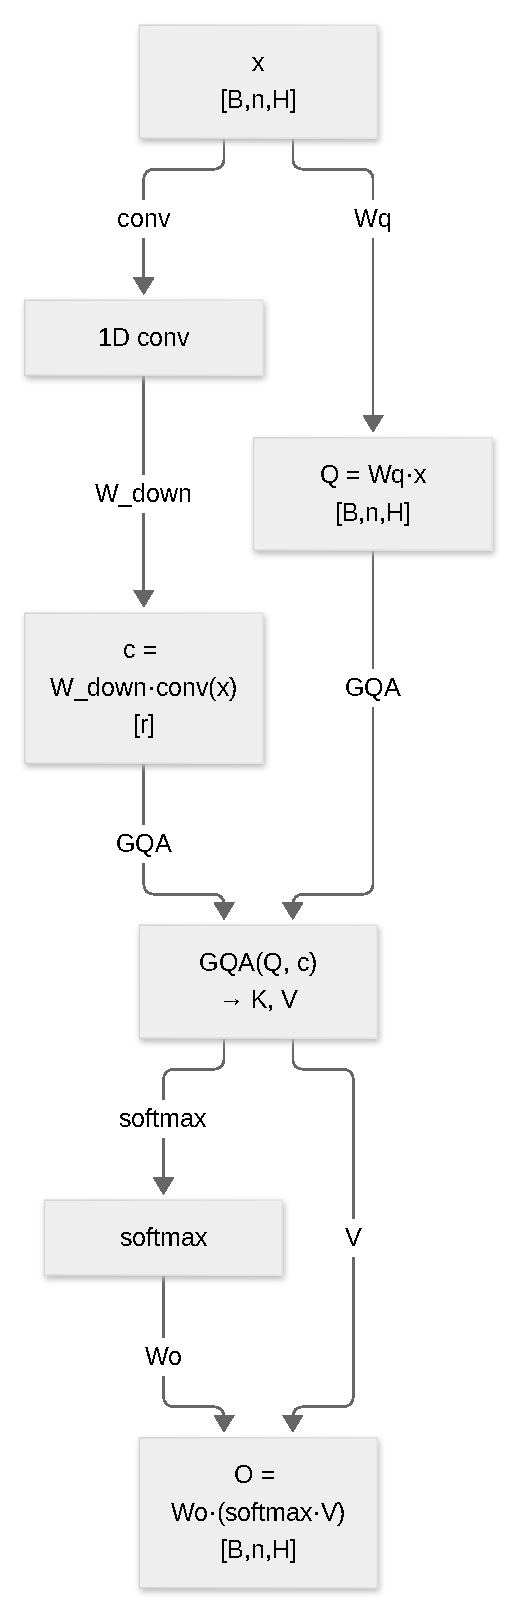
\includegraphics{figures/mixers/ccgqa.pdf}}
\caption{Dataflow of compressed convolutional grouped-query attention: the convolution latent supplies a grouped-query key/value expansion.}
\label{fig:mixer-ccgqa}
\end{figure}
Compressed Convolutional Grouped Query Attention (CCGQA) \citep{figliola_cca_2025} extends CCA with GQA-style key/value head sharing applied \emph{inside} the compressed latent, and \textbf{decouples} the query and KV compression rates: queries are compressed by $C_1$ and keys/values by $C_2 \geq C_1$. The per-head latent dimension $d_h$ must match between query and key heads, enforcing the constraint $C_2 / C_1 = n_h / n_{kv}$. KV heads are shared per group (replicated to match query heads), and the qk-mean bias uses broadcast/reduce operators $B_{\text{group}}$ (replicate KV heads to query heads) and $E_{\text{group}}$ (average query heads within each group). CCGQA achieves the best reported loss at 8$\times$ KV-cache compression with no quality drop versus MHA.

\subsubsection{Mathematical Formulation}
Same pipeline as CCA, with decoupled latents:
\[
\tilde{q}_{\text{pre}} = \tilde{W}_Q\, x \in \mathbb{R}^{E/C_1}, \qquad
\tilde{k}_{\text{pre}} = \tilde{W}_K\, x \in \mathbb{R}^{E/C_2}, \qquad C_2 \geq C_1.
\]
\[
\text{qk\_mean}_q = \tfrac{1}{2}(\tilde{q}_{\text{pre}} + B_{\text{group}}(\tilde{k}_{\text{pre}})), \qquad
\text{qk\_mean}_k = E_{\text{group}}(\text{qk\_mean}_q).
\]
\[
\text{attn} = \texttt{softmax}\!\left(\frac{\text{RoPE}(\hat{q})\, \text{RoPE}(\hat{k})^\top}{\sqrt{d_h}}\right) \tilde{v}, \qquad
\mathbf{Y} = \tilde{W}_O\, \text{attn}.
\]

\subsubsection{Key Characteristics}
\begin{itemize}[leftmargin=*]
    \item \textbf{Training complexity}: $\mathcal{O}(n^2 \cdot d / C_1)$ ($S^2$ term scales by $1/C_1$; projection terms by $1/C_1 + 1/C_2$).
    \item \textbf{Inference complexity}: $\mathcal{O}(n)$ per token, $\mathcal{O}(\tilde{e}_{kv} \cdot n)$ KV-cache space ($C_2$-compressed, group-shared).
    \item \textbf{Trainable}: $C_1$, $C_2$, $n_{kv}$, and all CCA tricks are configurable. Constraint: $C_2/C_1 = n_h/n_{kv}$.
    \item \textbf{Strengths}: Decoupled compression enables smooth Pareto frontier; same arithmetic intensity as GQA; best loss at 8$\times$ cache reduction.
    \item \textbf{Limitations}: Same quadratic $S^2$ (only reduced by $C_1$); fused kernel needed; two value projections add complexity.
\end{itemize}

The latent family shows a clear progression along two axes: (i) \textbf{rank compression}, moving from full heads (MHA) to a shared latent (MLA) to partitioned sub-head latents (MLRA), and (ii) \textbf{deployment adaptivity}, moving from a single decode path to hardware-adaptive dispatch (GQLA) and temporal cache merging (MTLA). Tucker Attention provides the unifying algebraic frame: MHA, GQA, and MLA are all special cases of a Tucker factorisation with appropriate rank choices. CCA and CCGQA take a fundamentally different approach: rather than compressing the KV-cache and then up-projecting for full-width attention (MLA/GQLA/MLRA), they perform attention \emph{entirely inside} the compressed latent space, reducing not just the cache but also the attention FLOPs by the compression factor. CCGQA further decouples query and KV compression rates, achieving the best reported loss at 8$\times$ KV-cache compression. Gaussian Mixture Attention (GMA) changes the routing philosophy entirely: instead of a low-rank linear bottleneck, it routes through $K$ learned probabilistic Gaussian components, achieving linear-time $\mathcal{O}(NK)$ sequence mixing for fixed $K$ while retaining a normalised attention-style interpretation.

\subsection{Gaussian Mixture Attention (GMA)}

\begin{figure}[H]
\centering
\fitfigure{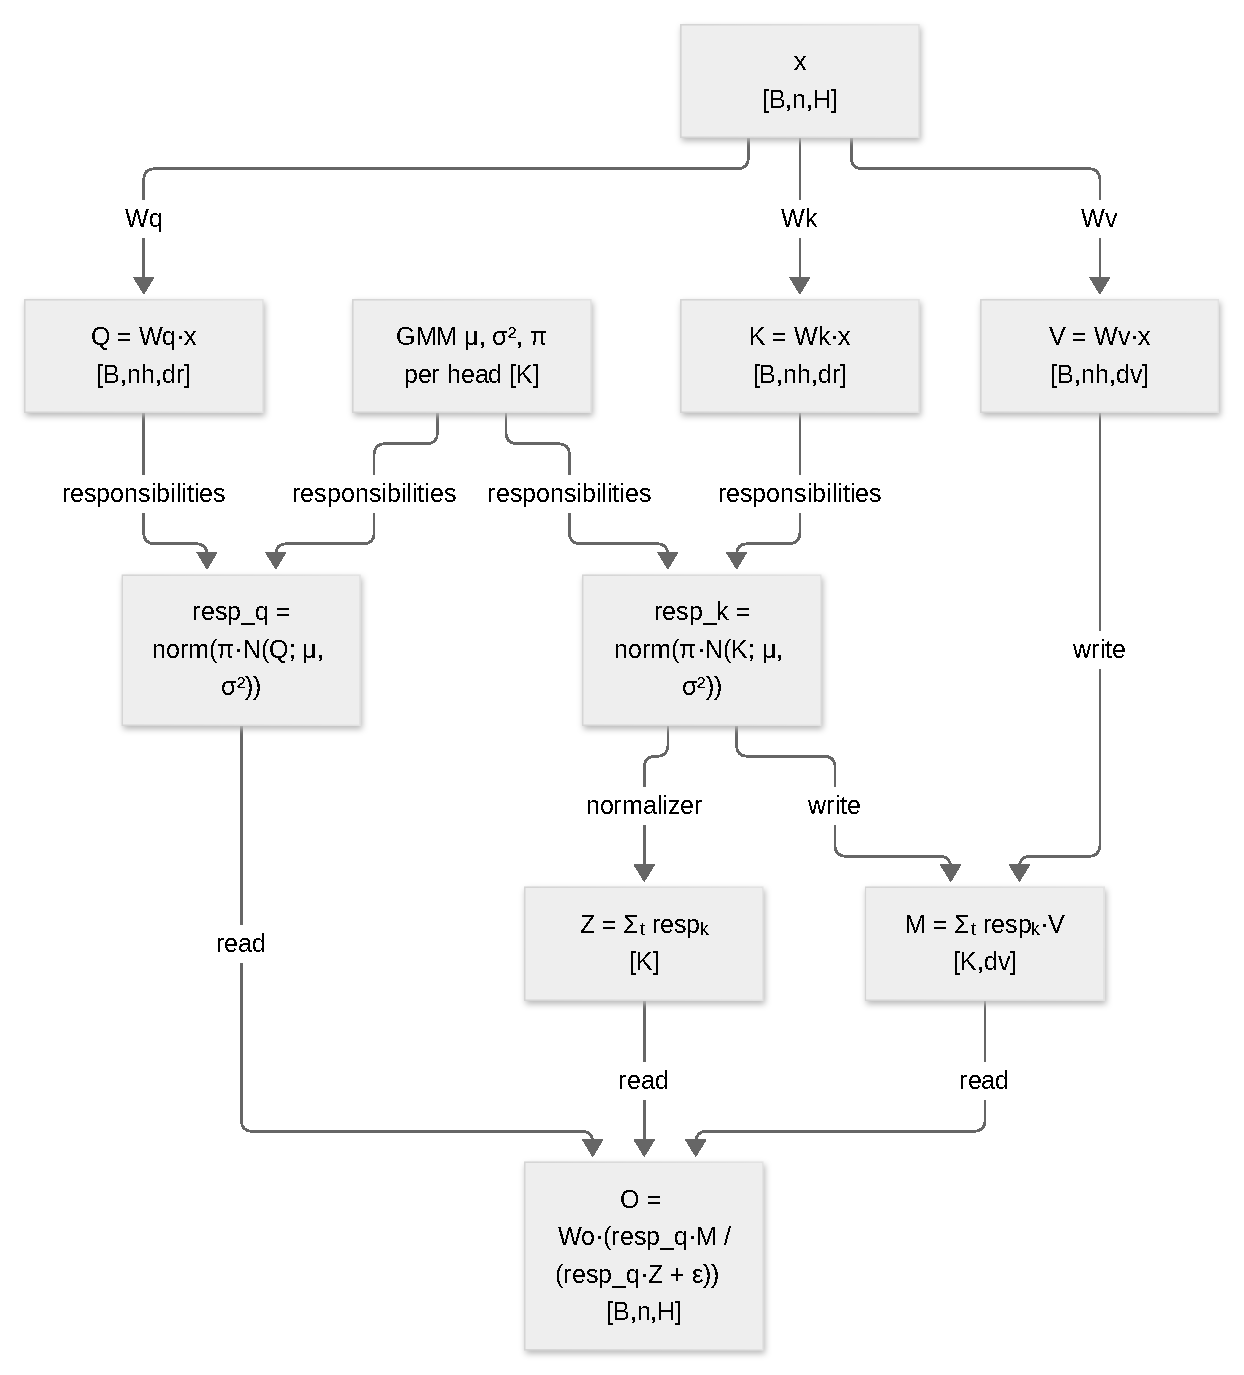
\includegraphics{figures/mixers/gma.pdf}}
\caption{Dataflow of Gaussian-mixture attention: per-head Gaussian responsibilities route keys and values into a $K$-slot memory that the query reads back, normalized by $Z$.}
\label{fig:mixer-gma}
\end{figure}
Gaussian Mixture Attention (GMA) \citep{huang_gma_2026} replaces the explicit pairwise $QK^\top$ interaction of standard dot-product attention with probabilistic routing through $K$ learned Gaussian-mixture components per head. Queries and keys are mapped to posterior \emph{responsibility} vectors over a shared latent routing space; their overlap defines an implicit responsibility-space affinity, while values are written into and read from a $K$-slot latent memory. By exploiting the associativity of matrix multiplication, GMA avoids materialising the induced $N \times N$ affinity matrix and instead uses two $N \times K$ responsibility matrices whose dominant activation storage scales as $\mathcal{O}(NK)$ rather than $\mathcal{O}(N^2)$ for fixed $K$. The Gaussian mixture parameters---component means $\mu$, diagonal covariances (reparameterised via $\sigma^2 = \text{softplus}(\omega) + \epsilon_\sigma$) and mixture-prior logits $\alpha$ (with $\pi = \text{softmax}(\alpha)$)---are fully differentiable learnable parameters optimised by standard backpropagation, with no EM loop or auxiliary clustering loss.

\subsubsection{Mathematical Formulation}
Per head, with routing dimension $d_r$ and value dimension $d_v$:
\[
Q_X = X W_Q \in \mathbb{R}^{N \times d_r}, \quad
K_X = X W_K \in \mathbb{R}^{N \times d_r}, \quad
V_X = X W_V \in \mathbb{R}^{N \times d_v}.
\]
The posterior responsibility of component $k$ for a routing vector $x_i$ is
\[
\gamma_{i,k} = p(z{=}k \mid x_i) = \frac{\pi_k\, \mathcal{N}(x_i \mid \mu_k, \Sigma_k)}{\sum_{\ell=1}^{K} \pi_\ell\, \mathcal{N}(x_i \mid \mu_\ell, \Sigma_\ell)},
\qquad \Sigma_k = \mathrm{diag}(\sigma_{k,1}^2, \dots, \sigma_{k,d_r}^2),
\]
yielding responsibility matrices $\Gamma^Q, \Gamma^K \in \mathbb{R}^{N \times K}$. The bidirectional output is computed by the associative write--read pair
\[
\tilde V = (\Gamma^K)^\top V_X \in \mathbb{R}^{K \times d_v}, \qquad
Z = (\Gamma^K)^\top \mathbf{1}_N \in \mathbb{R}^{K}, \qquad
O = \frac{\Gamma^Q \tilde V}{\Gamma^Q Z + \epsilon},
\]
which never materialises the implicit normalised affinity $A^{\text{GMA}}_{ij} = \frac{\sum_k \gamma^Q_{i,k} \gamma^K_{j,k}}{\sum_\ell \sum_k \gamma^Q_{i,k} \gamma^K_{\ell,k} + \epsilon}$. For autoregressive modelling the global write statistics are replaced by prefix-restricted cumulative sums $\tilde V^{(i)}_k = \sum_{j \le i} \gamma^K_{j,k} V_{X,j}$ and $Z^{(i)}_k = \sum_{j \le i} \gamma^K_{j,k}$, enforcing causality while preserving the fixed-$K$ linear scaling.

\subsubsection{Algorithmic Pseudocode}
\begin{algorithmic}[1]
\State \textbf{Input:} hidden state $X \in \mathbb{R}^{N \times d}$, $K$ components, routing dim $d_r$, value dim $d_v$, params $\{\mu_k, \omega_k, \alpha_k\}_{k=1}^{K}$
\State $Q_X \gets X W_Q$, \quad $K_X \gets X W_K$, \quad $V_X \gets X W_V$ \Comment{head projections}
\State $\sigma^2_k \gets \text{softplus}(\omega_k) + \epsilon_\sigma$, \quad $\pi_k \gets \text{softmax}(\alpha)_k$ \Comment{reparameterise}
\State $\Gamma^Q \gets \texttt{softmax}_k\!\left(\log \pi_k - \tfrac{d_r}{2}\log 2\pi - \tfrac{1}{2}\sum_m \log \sigma^2_{k,m} - \tfrac{1}{2}\sum_m \frac{(q_{i,m}-\mu_{k,m})^2}{\sigma^2_{k,m}}\right)$
\State $\Gamma^K \gets$ same as $\Gamma^Q$ applied to $K_X$
\If{causal}
    \State $\tilde V \gets \texttt{cumsum}_n(\Gamma^K \otimes V_X)$, \quad $Z \gets \texttt{cumsum}_n(\Gamma^K)$ \Comment{prefix-restricted}
\Else
    \State $\tilde V \gets (\Gamma^K)^\top V_X$, \quad $Z \gets (\Gamma^K)^\top \mathbf{1}_N$ \Comment{global write}
\EndIf
\State $O \gets \Gamma^Q \tilde V \,/\, (\Gamma^Q Z + \epsilon)$ \Comment{normalised read}
\State \textbf{Output:} $\mathbf{Y} = O W_O$
\end{algorithmic}

\subsubsection{Key Characteristics}
\begin{itemize}[leftmargin=*]
    \item \textbf{Training complexity}: $\mathcal{O}(N K d_r + N K d_v)$ for fixed $K$, linear in the sequence length $N$.
    \item \textbf{Inference complexity}: $\mathcal{O}(K)$ per token (responsibilities + latent read), $\mathcal{O}(NK)$ activation storage.
    \item \textbf{Trainable}: fully differentiable GMM parameters $\{\mu, \omega, \alpha\}$ per head, optimised end-to-end without EM.
    \item \textbf{Strengths}: Fixed-$K$ linear-time sequence mixing; probabilistic interpretable routing; bidirectional and causal variants; non-negative low-rank affinity interpretation $A^{\text{GMA}} = \mathrm{diag}(d)^{-1} \Gamma^Q (\Gamma^K)^\top$.
    \item \textbf{Limitations}: Quality depends on $K$ and the routing dimension $d_r$; causal GMA trails optimised SDPA and state-space models on WikiText-103 in the paper's current implementation; not a universal replacement for softmax attention.
\end{itemize}
\section{Comprehensive Sparse Attention Mechanisms}
\label{sec:annex-sparse}

\subsection{Executive Summary}

Sparse attention mechanisms address the prohibitive $\mathcal{O}(n^2)$ computational and memory complexity of standard scaled dot-product attention by restricting the set of attended key-value pairs. Modern sparse attention spans a rich design space distinguished by four orthogonal dimensions: (i) \textbf{sparsity pattern} (fixed geometric, data-dependent, or frequency-based), (ii) \textbf{trainability} (end-to-end trained or inference-only), (iii) \textbf{sparsity unit} (individual tokens, local windows, or blocks), and (iv) \textbf{mechanism} (masking, selection, filtering, or compression). This annex synthesizes seven major sparse attention families---Sparse Transformer, Longformer, BigBird, SparseK, NSA, SpargeAttn, and FASA---providing mathematical formulations, algorithmic pseudocode, and comprehensive architectural comparisons.

\subsection{Sparse Transformer: Factorized Strided and Fixed Patterns}

\begin{figure}[H]
\centering
\fitfigure{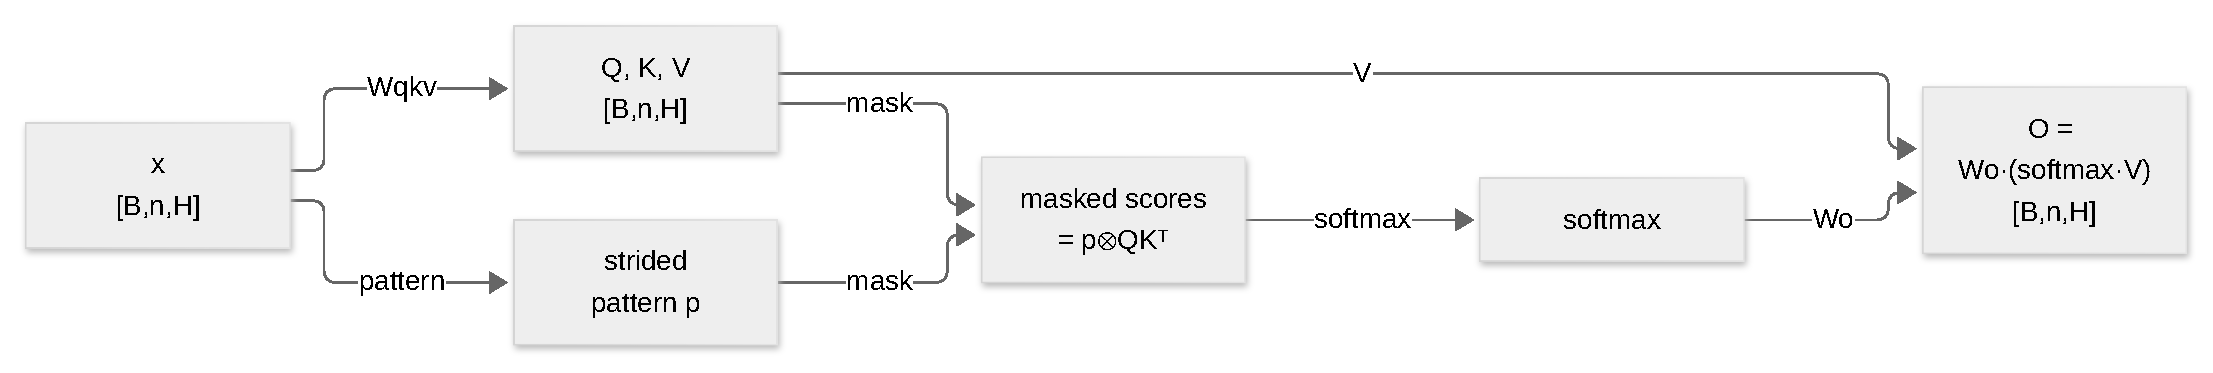
\includegraphics{figures/mixers/sparse-transformer.pdf}}
\caption{Dataflow of the Sparse Transformer: a strided factorized pattern masks the score matrix before softmax.}
\label{fig:mixer-sparse-transformer}
\end{figure}

\subsubsection{Mathematical Formulation}

The Sparse Transformer \citep{child_sparse_transformer_2019} reduces quadratic complexity to $\mathcal{O}(n\sqrt{n})$ by factorizing sparse attention into two complementary sparse heads. Let $n$ be the sequence length and $l = \lfloor\sqrt{n}\rfloor$ be the stride.

\paragraph{Strided attention head}: Each position $i$ attends to every $l$-th previous position:
\[
\mathcal{A}_i^{(\text{strided})} = \{j : j \leq i,\; (i - j) \bmod l = 0\}
\]

\paragraph{Fixed attention head}: Each position $i$ attends to positions within its local block plus fixed summary columns:
\[
\mathcal{A}_i^{(\text{fixed})} = \{j : \lfloor j/l \rfloor = \lfloor i/l \rfloor\} \cup \{j : j \bmod l \in \{l-c, \ldots, l-1\}\}
\]
where $c$ is a hyperparameter controlling the number of summary columns (typically $c=1$ or $c=2$).

The attention computation for each head $h$ follows standard scaled dot-product rules restricted to the sparse set:
\[
\text{Attn}_h(Q, K, V)_i = \text{softmax}\left(\frac{q_i^h K_{\mathcal{A}_i}^h\top}{\sqrt{d_k}}\right) V_{\mathcal{A}_i}^h
\]

The key insight is that with the two factorized heads operating in parallel across a depth of $L$ transformer layers, every position can reach every other position through a path of length at most $L + 1$, preserving long-range reachability with a fraction of dense attention cost.

\subsubsection{Algorithmic Pseudocode}

\begin{algorithm}[H]
\caption{Sparse Transformer Attention: Strided + Fixed Dual Heads}
\begin{algorithmic}[1]
\Require Query $\mathbf{Q} \in \mathbb{R}^{n \times d}$, Key $\mathbf{K} \in \mathbb{R}^{n \times d}$, Value $\mathbf{V} \in \mathbb{R}^{n \times d}$
\Require Stride $l = \lfloor\sqrt{n}\rfloor$, summary columns $c \in \{1, 2\}$
\Ensure Output $\mathbf{Y} \in \mathbb{R}^{n \times d}$
\State \textbf{Head 1: Strided Attention}
\For{$i = 1, \ldots, n$}
    \State $\mathcal{A}_i \gets \{j : j \leq i \text{ and } (i-j) \bmod l = 0\}$ \Comment{Every $l$-th position}
    \State $\text{scores}_{i} \gets \mathbf{q}_i \mathbf{K}_{\mathcal{A}_i}^\top / \sqrt{d_k}$
    \State $\text{attn}_{i} \gets \text{softmax}(\text{scores}_{i})$
    \State $\mathbf{y}_i^{(1)} \gets \text{attn}_{i} \mathbf{V}_{\mathcal{A}_i}$
\EndFor
\State \textbf{Head 2: Fixed Block + Summary Attention}
\For{$i = 1, \ldots, n$}
    \State $\text{block\_start} \gets \lfloor i/l \rfloor \cdot l$, $\text{block\_end} \gets \min(i+1, \text{block\_start}+l)$
    \State $\mathcal{A}_i \gets [\text{block\_start}, \text{block\_end}) \cup \{\text{cols from last } c \text{ columns}\}$
    \State $\text{scores}_{i} \gets \mathbf{q}_i \mathbf{K}_{\mathcal{A}_i}^\top / \sqrt{d_k}$
    \State $\text{attn}_{i} \gets \text{softmax}(\text{scores}_{i})$
    \State $\mathbf{y}_i^{(2)} \gets \text{attn}_{i} \mathbf{V}_{\mathcal{A}_i}$
\EndFor
\State Concatenate: $\mathbf{Y} = [\mathbf{y}^{(1)} \| \mathbf{y}^{(2)}]$ and project via output linear layer
\Return $\mathbf{Y}$
\end{algorithmic}
\end{algorithm}

\subsubsection{Key Characteristics}

\begin{itemize}[leftmargin=*]
    \item \textbf{Complexity}: $\mathcal{O}(n\sqrt{n} \cdot d)$ during training; $\mathcal{O}(n)$ per token during generation.
    \item \textbf{Trainable}: Yes; full backpropagation through selected positions.
    \item \textbf{Sparsity pattern}: Fixed and data-agnostic; patterns do not adapt to content.
    \item \textbf{Strength}: Structured reachability guarantees long-range dependencies; proven effective on long sequences (Enwik8, text images).
    \item \textbf{Limitation}: Fixed patterns may miss important but non-contiguous relationships; requires custom CUDA kernels for practical efficiency.
\end{itemize}

\subsection{Longformer: Sliding Window, Dilation, and Global Tokens}

\begin{figure}[H]
\centering
\fitfigure{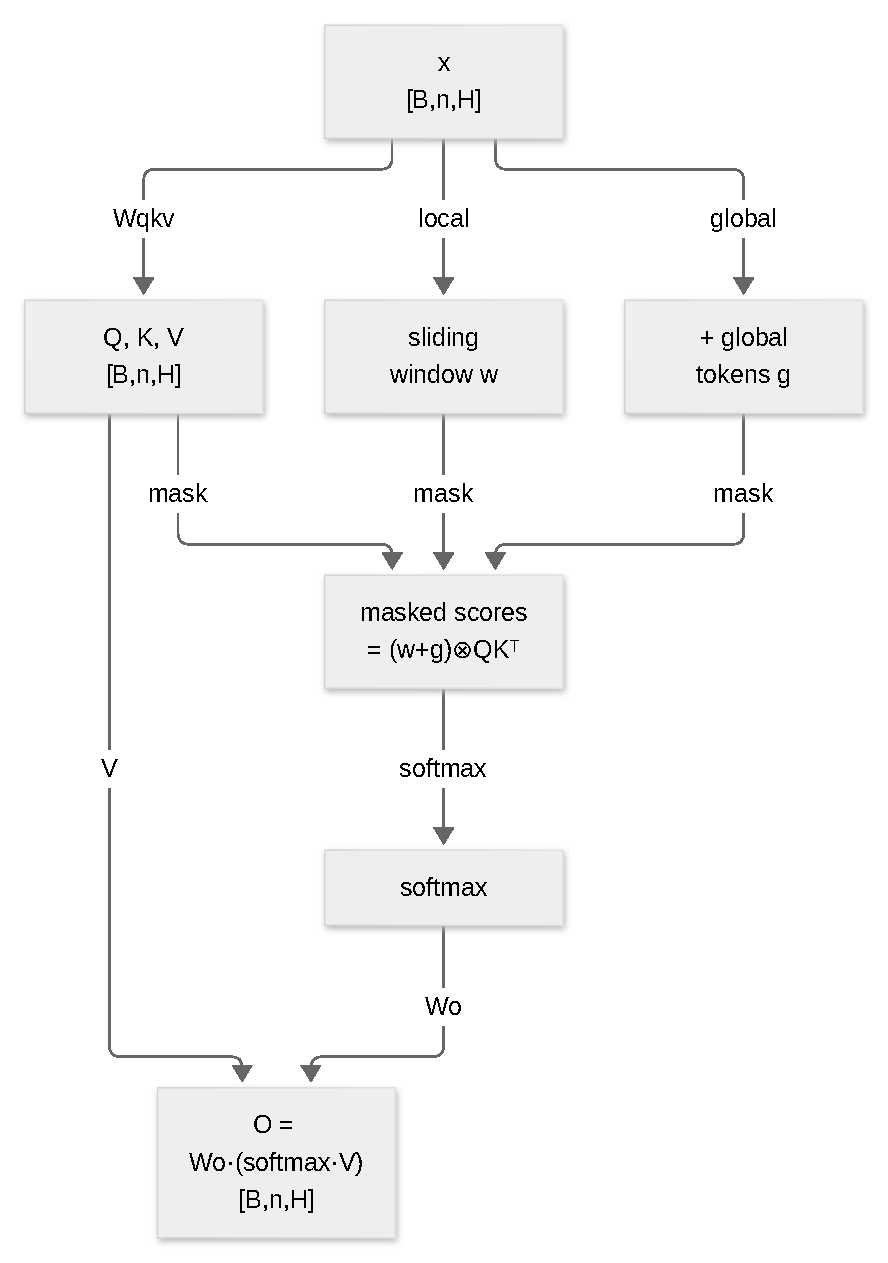
\includegraphics{figures/mixers/longformer.pdf}}
\caption{Dataflow of Longformer: sliding-window and global-token masks are applied to the score matrix before softmax.}
\label{fig:mixer-longformer}
\end{figure}

\subsubsection{Mathematical Formulation}

Longformer \citep{beltagy_longformer_2020} achieves linear $\mathcal{O}(n \cdot w)$ complexity by combining three complementary attention patterns.

\paragraph{Sliding window attention}: Local neighborhood of size $w$:
\[
\mathcal{A}_i^{(\text{window})} = \{j : |i - j| \leq w/2\}
\]

\paragraph{Dilated sliding window}: Windowed attention with dilation $d$, skipping stride $d+1$:
\[
\mathcal{A}_i^{(\text{dilated})} = \{j : |i - j| \leq (w/2)(d+1) \text{ and } (i-j) \bmod (d+1) = 0\}
\]

\paragraph{Global attention}: Designated global tokens (e.g., $[\text{CLS}]$) attend to all positions and are attended by all:
\[
\mathcal{A}_i^{(\text{global})} = \begin{cases}
\{1, \ldots, n\} & \text{if } i \in \mathcal{G} \\
\mathcal{A}_i^{(\text{window})} \cup \mathcal{G} & \text{otherwise}
\end{cases}
\]

The three patterns are applied via separate projections. The local and global attention can use either the same projections or task-specific separate ones.

\subsubsection{Algorithmic Pseudocode}

\begin{algorithm}[H]
\caption{Longformer: Sliding Window + Dilated + Global}
\begin{algorithmic}[1]
\Require Query $\mathbf{Q} \in \mathbb{R}^{n \times d}$, Key $\mathbf{K}$, Value $\mathbf{V}$, window size $w$, dilation $d$, global token indices $\mathcal{G}$
\Ensure Output $\mathbf{Y}$
\For{$i = 1, \ldots, n$}
    \If{$i \in \mathcal{G}$}
        \State $\mathcal{A}_i \gets \{1, \ldots, n\}$ \Comment{Global token attends to all}
    \Else
        \State Local window: $\mathcal{A}^{(\text{local})} \gets [i - w/2, i + w/2] \cap [1, n]$
        \State Dilated offsets: $\mathcal{A}^{(\text{dilated})} \gets \{j : (i-j) \bmod (d+1) = 0\} \cap \mathcal{A}^{(\text{dilated range})}$
        \State Combine: $\mathcal{A}_i \gets \mathcal{A}^{(\text{local})} \cup \mathcal{A}^{(\text{dilated})} \cup \mathcal{G}$
    \EndIf
    \State $\text{scores}_i \gets \mathbf{q}_i \mathbf{K}_{\mathcal{A}_i}^\top / \sqrt{d_k}$
    \State $\text{attn}_i \gets \text{softmax}(\text{scores}_i)$
    \State $\mathbf{y}_i \gets \text{attn}_i \mathbf{V}_{\mathcal{A}_i}$
\EndFor
\Return $\mathbf{Y}$
\end{algorithmic}
\end{algorithm}

\subsubsection{Key Characteristics}

\begin{itemize}[leftmargin=*]
    \item \textbf{Complexity}: $\mathcal{O}(n \cdot w)$ where $w$ is the window size (linear when $w \ll n$).
    \item \textbf{Trainable}: Yes; drop-in replacement for standard attention.
    \item \textbf{Coverage}: With $L$ layers and window size $w$, receptive field grows to $L \times w$, covering entire sequence with shallow networks.
    \item \textbf{Strength}: Practical for document-level tasks; dilation expands local receptive fields with minimal overhead; global tokens provide query-document correspondence.
    \item \textbf{Limitation}: Window size remains a design hyperparameter; suboptimal for tasks requiring dense attention patterns.
\end{itemize}

\subsection{BigBird: Random, Local, and Global Sparse Graph}

\begin{figure}[H]
\centering
\fitfigure{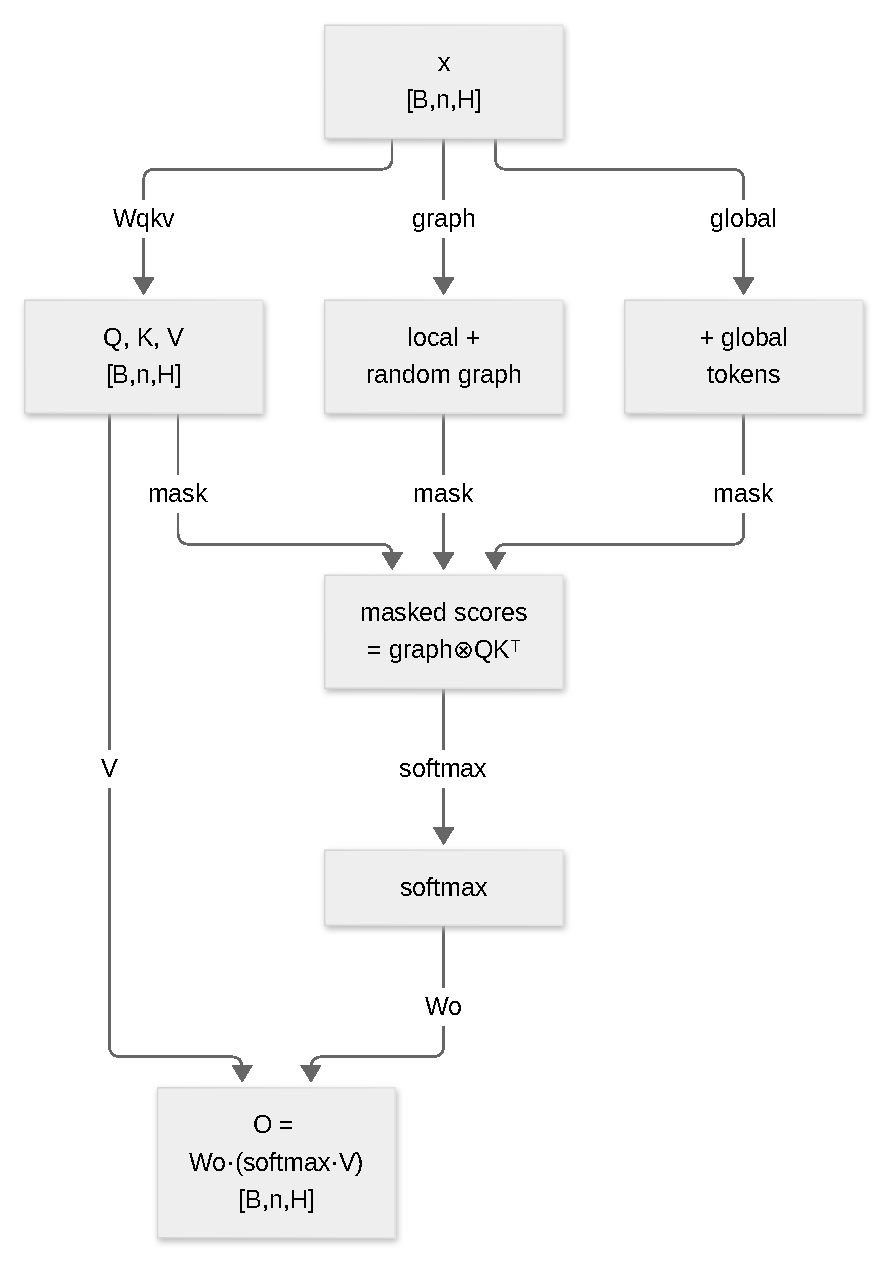
\includegraphics{figures/mixers/bigbird.pdf}}
\caption{Dataflow of BigBird: local, random, and global adjacency masks the score matrix before softmax.}
\label{fig:mixer-bigbird}
\end{figure}

\subsubsection{Mathematical Formulation}

BigBird \citep{zaheer_bigbird_2020} preserves universal approximation and Turing completeness using a principled mix of three sparsity patterns.

\paragraph{Random connections}: Each position connects to $r$ randomly sampled positions:
\[
\mathcal{A}_i^{(\text{random})} = \text{RandomSample}(\{1, \ldots, n\}, r)
\]

\paragraph{Local window}: Sliding window neighborhood:
\[
\mathcal{A}_i^{(\text{local})} = \{j : |i-j| \leq w/2\}
\]

\paragraph{Global tokens}: Task-specific global anchors:
\[
\mathcal{A}_i^{(\text{global})} = \begin{cases}
\{1, \ldots, n\} & \text{if } i \in \mathcal{G} \\
\mathcal{A}_i^{(\text{random})} \cup \mathcal{A}_i^{(\text{local})} \cup \mathcal{G} & \text{otherwise}
\end{cases}
\]

The composite sparse mask $M$ is:
\[
M_{ij} = \mathbf{1}[j \in \mathcal{A}_i^{(\text{random})} \cup \mathcal{A}_i^{(\text{local})} \cup \mathcal{A}_i^{(\text{global})}]
\]

In practice, BigBird groups tokens into blocks of size $b$ and applies the sparsity decision at the block level, enabling efficient block-sparse implementations.

\subsubsection{Theoretical Guarantee}

The authors prove that with $O(1)$ random connections and global tokens, the sparse graph maintains the same universal approximation and Turing completeness properties as dense attention. Formally, any computable function can be represented and any sequence of operations can be simulated within the BigBird connectivity graph.

\subsubsection{Algorithmic Pseudocode}

\begin{algorithm}[H]
\caption{BigBird: Random + Local + Global Block-Sparse Attention}
\begin{algorithmic}[1]
\Require Query $\mathbf{Q}$, Key $\mathbf{K}$, Value $\mathbf{V}$, block size $b$, random links per block $r$, global indices $\mathcal{G}$
\Ensure Output $\mathbf{Y}$
\State Reshape into blocks: $n_b = \lceil n / b \rceil$ blocks
\For{block $i = 0, \ldots, n_b-1$}
    \For{position $j$ in block $i$}
        \State \textbf{Local window}: $\mathcal{A}_j^{(\text{local})} = \text{nearby positions in block} \cup \text{boundary positions}$
        \State \textbf{Random block sampling}: Sample $r$ blocks uniformly at random, add all positions from those blocks
        \State \textbf{Global}: Add all global token positions
        \State $\mathcal{A}_j \gets \mathcal{A}_j^{(\text{local})} \cup \mathcal{A}_j^{(\text{random})} \cup \mathcal{G}$
    \EndFor
\EndFor
\For{$i = 1, \ldots, n$}
    \State $\text{scores}_i \gets \mathbf{q}_i \mathbf{K}_{\mathcal{A}_i}^\top / \sqrt{d_k}$
    \State $\text{attn}_i \gets \text{softmax}(\text{scores}_i)$
    \State $\mathbf{y}_i \gets \text{attn}_i \mathbf{V}_{\mathcal{A}_i}$
\EndFor
\Return $\mathbf{Y}$
\end{algorithmic}
\end{algorithm}

\subsubsection{Key Characteristics}

\begin{itemize}[leftmargin=*]
    \item \textbf{Complexity}: $\mathcal{O}(n)$ or near-linear in optimal block-sparse implementation.
    \item \textbf{Trainable}: Yes.
    \item \textbf{Theoretical grounding}: Provably maintains universal approximation and Turing-completeness with sparse connectivity.
    \item \textbf{Strength}: Strong long-document performance on question answering, summarization, and genomics tasks.
    \item \textbf{Limitation}: Random sampling introduces variance and non-determinism; tuning of $r, w, g$ hyperparameters remains task-dependent.
\end{itemize}

\subsection{SparseK Attention: Differentiable \texorpdfstring{Top-$k$}{Top-k} Selection}

\begin{figure}[H]
\centering
\fitfigure{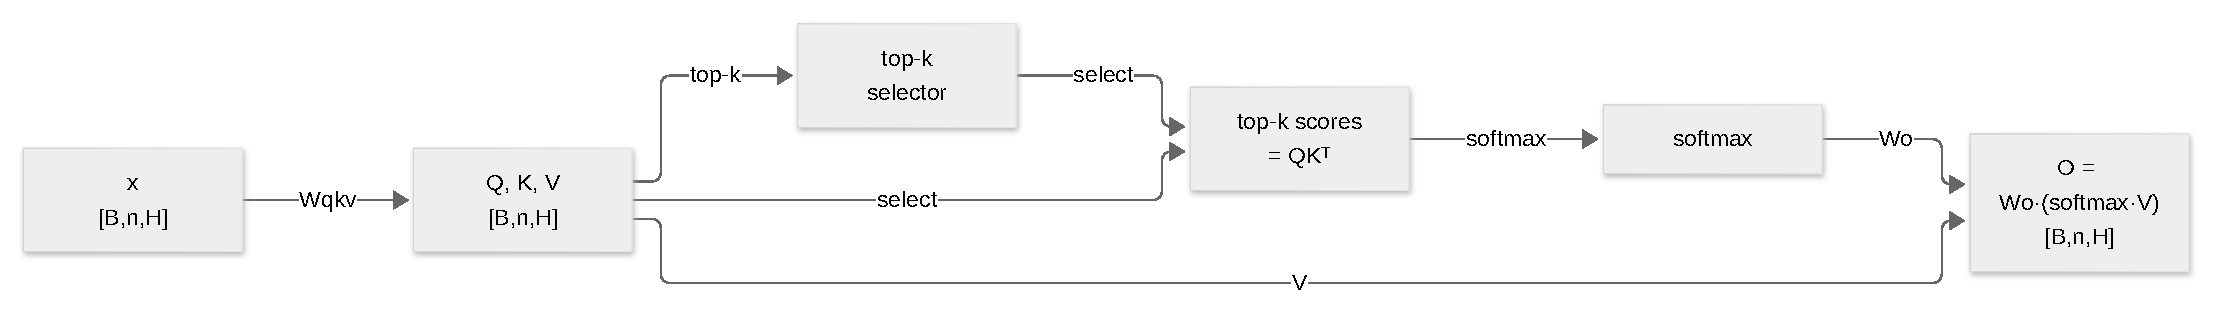
\includegraphics{figures/mixers/sparsek.pdf}}
\caption{Dataflow of SparseK: a differentiable top-$k$ selector keeps only the highest-scoring keys before softmax.}
\label{fig:mixer-sparsek}
\end{figure}

\subsubsection{Mathematical Formulation}

SparseK \citep{lou_sparsek_2024} enables learnable sparsity via a \textbf{differentiable top-$k$ operator}. A scoring network $\phi_\theta$ evaluates key-value pair importance:

\[
u_j = \phi_\theta(\mathbf{k}_j, \mathbf{q}_i) \in \mathbb{R}
\]

The \textbf{SparseK operator} selects the top-$k$ scores while remaining differentiable. It computes a threshold $\tau(u)$ such that the sum of active scores equals $k$:

\[
\text{SparseK}(u, k)_j = \max(u_j - \tau(u), 0), \quad \text{where} \quad \sum_j \max(u_j - \tau, 0) = k
\]

The threshold $\tau$ is found via bisection. The attention becomes:

\[
m_j = \text{SparseK}(u, k)_j, \quad \text{Attn}_i = \text{softmax}\left(\frac{\mathbf{q}_i K_{\text{sel}}^\top}{\sqrt{d_k}}\right) V_{\text{sel}}
\]

where $K_{\text{sel}}, V_{\text{sel}}$ contain only the top-$k$ entries (those with $m_j > 0$).

\subsubsection{Algorithmic Pseudocode}

\begin{algorithm}[H]
\caption{SparseK: Differentiable Top-$k$ Attention}
\begin{algorithmic}[1]
\Require Query $\mathbf{q} \in \mathbb{R}^d$, Key matrix $\mathbf{K} \in \mathbb{R}^{n \times d}$, Value matrix $\mathbf{V} \in \mathbb{R}^{n \times d}$
\Require Scoring network $\phi_\theta$, target sparsity $k$
\Ensure Attention output $\mathbf{y}$
\State \textbf{Compute importance scores:}
\For{$j = 1, \ldots, n$}
    \State $u_j \gets \phi_\theta(\mathbf{k}_j, \mathbf{q})$
\EndFor
\State \textbf{Compute differentiable top-$k$ via threshold:}
\State $u_{\text{sorted}} \gets \text{sort}(u, \text{descending}=\text{True})$
\State $\text{cumsum} \gets \text{cumsum}(u_{\text{sorted}})$
\State Find $\rho = \max\{i : u_{\text{sorted}}[i] > 0 \text{ and cumsum}[i] \leq k\}$
\State $\tau \gets (u_{\text{sorted}}[\rho] - k) / (\rho + 1)$ \Comment{Threshold for $k$ active elements}
\State $m \gets \max(u - \tau, 0)$ \Comment{Differentiable selection mask}
\State \textbf{Apply mask and compute attention:}
\State $K_{\text{sel}} \gets K[m > 0]$, $V_{\text{sel}} \gets V[m > 0]$
\State $\text{scores} \gets \mathbf{q} K_{\text{sel}}^\top / \sqrt{d_k}$
\State $\text{attn} \gets \text{softmax}(\text{scores})$
\State $\mathbf{y} \gets \text{attn} \cdot V_{\text{sel}}$
\Return $\mathbf{y}$
\end{algorithmic}
\end{algorithm}

\subsubsection{Key Characteristics}

\begin{itemize}[leftmargin=*]
    \item \textbf{Complexity}: $\mathcal{O}(n \cdot d)$ during training (linear in sequence length); $\mathcal{O}(k)$ per token during generation.
    \item \textbf{Trainable}: Yes; end-to-end gradient flow through the SparseK operator.
    \item \textbf{Incremental generation}: Supports efficient constant-memory autoregressive generation.
    \item \textbf{Strength}: Seamlessly integrates into existing LLM architectures; minimal fine-tuning needed.
    \item \textbf{Limitation}: Scattered memory access from top-$k$ selection may limit cache efficiency on some hardware; scoring network adds overhead.
\end{itemize}

\subsection{NSA (Native Sparse Attention): Hardware-Aligned Hierarchical Branches}

\begin{figure}[H]
\centering
\fitfigure{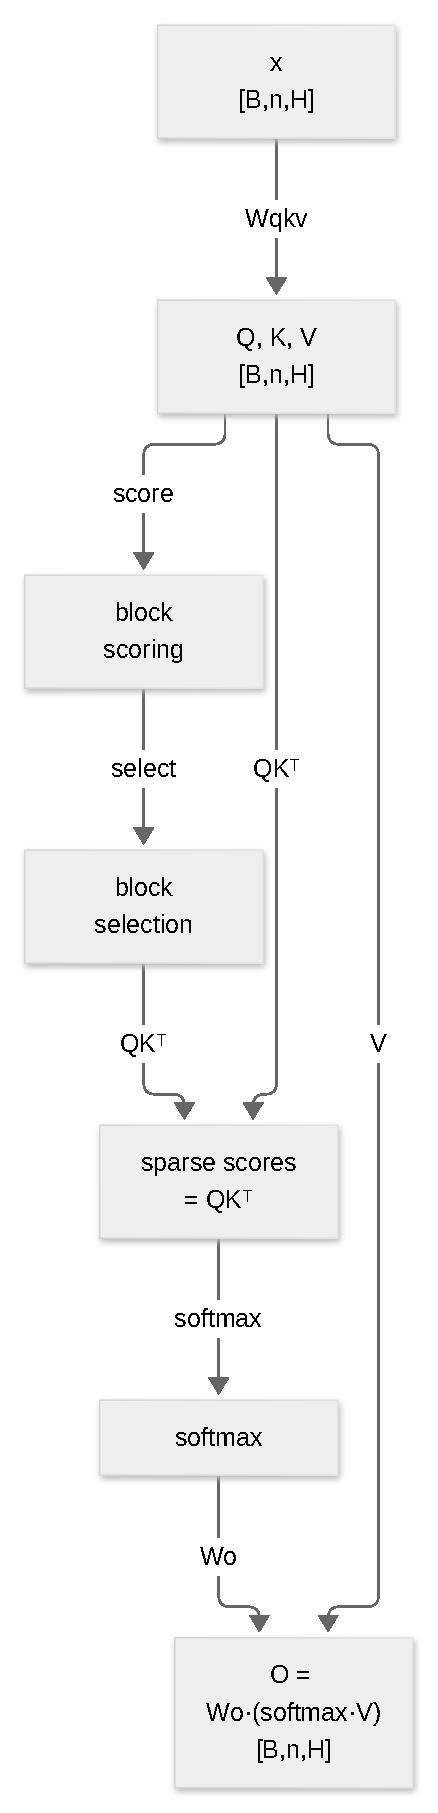
\includegraphics{figures/mixers/nsa.pdf}}
\caption{Dataflow of NSA: hierarchical block scoring and selection restrict the score matrix to selected blocks.}
\label{fig:mixer-nsa}
\end{figure}

\subsubsection{Mathematical Formulation}

NSA \citep{yuan_nsa_2025} decomposes sparse attention into three parallel branches that are combined through learned gates.

\paragraph{Compression branch}: A learnable MLP $\varphi$ compresses key-value blocks:

\[
\tilde{K}_t^{\text{cmp}} = \left[\varphi(k_{id+1:id+l})\right]_{\substack{1 \leq i \leq \lfloor(t-l)/d\rfloor}} \quad, \quad \tilde{V}_t^{\text{cmp}} = \left[\varphi(v_{id+1:id+l})\right]
\]

\paragraph{Selection branch}: High-importance blocks are selected based on compressed scores:

\[
p_t^{\text{cmp}} = \text{softmax}(q_t^\top \tilde{K}_t^{\text{cmp}} / \sqrt{d}), \quad I_t = \mathrm{TopK}(p_t^{\text{cmp}}, n), \quad \tilde{K}_t^{\text{sel}} = \mathrm{Gather}(K, I_t)
\]

\paragraph{Sliding window branch}: Fixed local context:

\[
\tilde{K}_t^{\text{win}} = K_{t-w:t}, \quad \tilde{V}_t^{\text{win}} = V_{t-w:t}
\]

\paragraph{Gated combination}: The three attention outputs are combined via learned gates:

\[
\alpha_t^{(\text{cmp})} = \sigma(\text{Linear}_\text{cmp}(q_t)), \quad \alpha_t^{(\text{sel})} = \sigma(\text{Linear}_\text{sel}(q_t)), \quad \alpha_t^{(\text{win})} = \sigma(\text{Linear}_\text{win}(q_t))
\]

\[
y_t = \alpha_t^{(\text{cmp})} \cdot \text{Attn}(q_t, \tilde{K}^{\text{cmp}}, \tilde{V}^{\text{cmp}}) + \alpha_t^{(\text{sel})} \cdot \text{Attn}(q_t, \tilde{K}^{\text{sel}}, \tilde{V}^{\text{sel}}) + \alpha_t^{(\text{win})} \cdot \text{Attn}(q_t, \tilde{K}^{\text{win}}, \tilde{V}^{\text{win}})
\]

\subsubsection{Algorithmic Pseudocode}

\begin{algorithm}[H]
\caption{NSA: Compressed + Selected + Window Branches with Learned Gating}
\begin{algorithmic}[1]
\Require Query $\mathbf{q}_t$, cached Key/Value sequences, block size $l$, stride $d$, selection count $n$, window $w$
\Require Compression MLP $\varphi$, gate networks $\text{Linear}_{\text{cmp}}, \text{Linear}_{\text{sel}}, \text{Linear}_{\text{win}}$
\Ensure Output $\mathbf{y}_t$
\State \textbf{Compression branch:}
\For{$i = 1$ to $\lfloor t/d \rfloor$}
    \State $k_i^{\text{cmp}} \gets \varphi(\mathbf{K}_{id+1:id+l})$ \Comment{Compress block via MLP}
    \State $v_i^{\text{cmp}} \gets \varphi(\mathbf{V}_{id+1:id+l})$
\EndFor
\State $\tilde{\mathbf{K}}^{\text{cmp}} \gets [k_1^{\text{cmp}}, \ldots, k_{\lfloor t/d \rfloor}^{\text{cmp}}]$, $\tilde{\mathbf{V}}^{\text{cmp}} \gets [v_1^{\text{cmp}}, \ldots, v_{\lfloor t/d \rfloor}^{\text{cmp}}]$
\State $\mathbf{y}_t^{(\text{cmp})} \gets \text{SDPA}(\mathbf{q}_t, \tilde{\mathbf{K}}^{\text{cmp}}, \tilde{\mathbf{V}}^{\text{cmp}})$
\State \textbf{Selection branch:}
\State Compute scores on compressed: $\mathbf{s} \gets \text{softmax}(\mathbf{q}_t \tilde{\mathbf{K}}^{\text{cmp}\top} / \sqrt{d})$
\State Select top-$n$ important blocks: $I \gets \mathrm{TopK}(\mathbf{s}, n)$
\State Gather full blocks: $\tilde{\mathbf{K}}^{\text{sel}} \gets [\mathbf{K}_{I_i d+1:I_i d+l}]_i$, $\tilde{\mathbf{V}}^{\text{sel}} \gets [\mathbf{V}_{I_i d+1:I_i d+l}]_i$
\State $\mathbf{y}_t^{(\text{sel})} \gets \text{SDPA}(\mathbf{q}_t, \tilde{\mathbf{K}}^{\text{sel}}, \tilde{\mathbf{V}}^{\text{sel}})$
\State \textbf{Window branch:}
\State $\mathbf{y}_t^{(\text{win})} \gets \text{SDPA}(\mathbf{q}_t, \mathbf{K}_{t-w:t}, \mathbf{V}_{t-w:t})$
\State \textbf{Gated fusion:}
\State $\alpha^{(\text{cmp})} \gets \sigma(\text{Linear}_{\text{cmp}}(\mathbf{q}_t))$, $\alpha^{(\text{sel})} \gets \sigma(\text{Linear}_{\text{sel}}(\mathbf{q}_t))$, $\alpha^{(\text{win})} \gets \sigma(\text{Linear}_{\text{win}}(\mathbf{q}_t))$
\State $\mathbf{y}_t \gets \alpha^{(\text{cmp})} \mathbf{y}_t^{(\text{cmp})} + \alpha^{(\text{sel})} \mathbf{y}_t^{(\text{sel})} + \alpha^{(\text{win})} \mathbf{y}_t^{(\text{win})}$
\Return $\mathbf{y}_t$
\end{algorithmic}
\end{algorithm}

\subsubsection{Key Characteristics}

\begin{itemize}[leftmargin=*]
    \item \textbf{Complexity}: $\mathcal{O}(t/d + n \cdot l + w)$ tokens attended per step (significantly reduced versus $\mathcal{O}(t)$ for dense).
    \item \textbf{Trainable}: Yes; direct training with all branches differentiable.
    \item \textbf{Hardware alignment}: Designed for efficient tensor core utilization; compression and selection reduce memory bandwidth pressure.
    \item \textbf{Strength}: 11.6$\times$ decoding speedup and 9$\times$ forward speedup on 64k sequences; outperforms full attention on many tasks.
    \item \textbf{Limitation}: Requires custom Triton/CUDA kernels; complex multi-branch architecture increases engineering overhead.
\end{itemize}

\subsection{FASA: Frequency-Aware Sparse Attention}

\begin{figure}[H]
\centering
\fitfigure{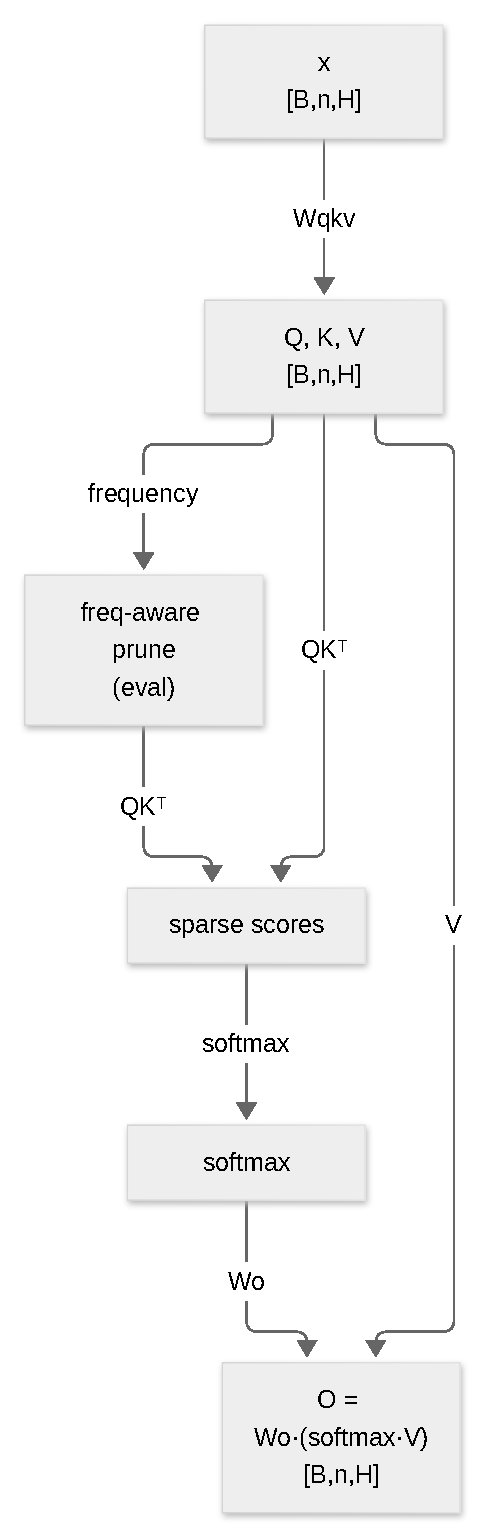
\includegraphics{figures/mixers/fasa.pdf}}
\caption{Dataflow of FASA: a frequency-aware prune stage (evaluation only) drops low-value key blocks before softmax.}
\label{fig:mixer-fasa}
\end{figure}

\subsubsection{Mathematical Formulation}

FASA \citep{wang_fasa_2026} is a \textbf{training-free inference-time method} that exploits rotary position embedding (RoPE) structure. Under RoPE, the token embedding is rotated by $\theta_i = B^{-2(i-1)/d}$, decomposing the $d$-dimensional space into $d/2$ frequency chunks (FCs).

\paragraph{Key insight}: Only a small subset ($ < 1\%$) of FCs matter for contextual awareness; most encode positional patterns.

\paragraph{Dominant frequency chunk identification}: For each layer $l$ and head $h$, identify dominant FCs via contextual agreement (CA):

\[
\text{CA}^{l,h,i} = \frac{|\text{TopK}(\alpha^{l,h}) \cap \text{TopK}(\alpha^{l,h,i})|}{K}
\]

where $\alpha^{l,h}$ is the full attention mask and $\alpha^{l,h,i}$ is the mask using only FC $i$. Dominant FCs have high CA---they contribute meaningfully to the final attention pattern.

\paragraph{Token importance prediction (TIP) stage}: Using only dominant FCs, compute lightweight importance per token:

\[
S_t^{l,h} = \sum_{i \in \mathcal{I}_{\text{dom}}^{l,h}} \alpha^{l,h,i}(\mathbf{q}_t, \mathbf{K}_{1:t}), \quad \mathcal{T}_t = \text{TopK-Indices}(S_t, N_{\text{fac}})
\]

\paragraph{Focused attention computation (FAC) stage}: Compute full-precision attention on selected tokens:

\[
\hat{\alpha}_{\text{FAC}} = \text{softmax}\left(\frac{\mathbf{q}_t \mathbf{K}_{\mathcal{T}_t}^\top}{\sqrt{d}}\right), \quad \mathbf{o}_t = \hat{\alpha}_{\text{FAC}} \mathbf{V}_{\mathcal{T}_t}
\]

\subsubsection{Algorithmic Pseudocode}

\begin{algorithm}[H]
\caption{FASA: Frequency-Aware Sparse Attention (Inference-Time)}
\begin{algorithmic}[1]
\Require Current query $\mathbf{q}_t$, cached Key/Value $\mathbf{K}_{1:t}, \mathbf{V}_{1:t}$, RoPE base $B$, dominant FCs $\mathcal{I}_{\text{dom}}$
\Require TIP token budget $N_{\text{tip}}$, FAC token budget $N_{\text{fac}}$
\Ensure Output $\mathbf{o}_t$
\State \textbf{Stage 1: Token Importance Prediction (TIP)}
\For{layer $l$ and head $h$}
    \For{position $i = 1$ to $t$}
        \State Compute importance from dominant FCs: $s_i \gets 0$
        \For{$fc \in \mathcal{I}_{\text{dom}}^{l,h}$}
            \State Rotate query and key into FC $fc$: $\mathbf{q}^{(fc)}, \mathbf{k}_i^{(fc)}$
            \State $s_i^{(fc)} \gets \text{softmax}(\mathbf{q}^{(fc)} \mathbf{k}_i^{(fc)\top} / \sqrt{d}) $
            \State $s_i \gets s_i + s_i^{(fc)}$
        \EndFor
    \EndFor
    \State $\mathcal{T}_t \gets \mathrm{TopK-Indices}([s_1, \ldots, s_t], N_{\text{fac}})$ \Comment{Select top tokens}
\EndFor
\State \textbf{Stage 2: Focused Attention Computation (FAC)}
\State $\text{scores}_{\text{fac}} \gets \mathbf{q}_t \mathbf{K}_{\mathcal{T}_t}^\top / \sqrt{d}$ \Comment{Full-precision dot product}
\State $\alpha_{\text{fac}} \gets \text{softmax}(\text{scores}_{\text{fac}})$ \Comment{Full softmax}
\State $\mathbf{o}_t \gets \alpha_{\text{fac}} \mathbf{V}_{\mathcal{T}_t}$ \Comment{Weighted value sum}
\Return $\mathbf{o}_t$
\end{algorithmic}
\end{algorithm}

\subsubsection{Key Characteristics}

\begin{itemize}[leftmargin=*]
    \item \textbf{Complexity}: TIP is $\mathcal{O}(t \cdot N_{\text{tip}})$; FAC is $\mathcal{O}(N_{\text{fac}} \cdot d)$.
    \item \textbf{Trainable}: No; training-free inference optimization.
    \item \textbf{Applicability}: Requires RoPE-based models; extended to ALiBi and MLA with modifications.
    \item \textbf{Strength}: Near-oracle accuracy with $\leq 256$ tokens out of millions; up to 2.56$\times$ decoding speedup; orthogonal to quantization.
    \item \textbf{Limitation}: Offline offline calibration required; dominant FC identification adds preprocessing overhead.
\end{itemize}

\subsection{SpargeAttn: Two-Stage Block-Level Filtering}

\begin{figure}[H]
\centering
\fitfigure{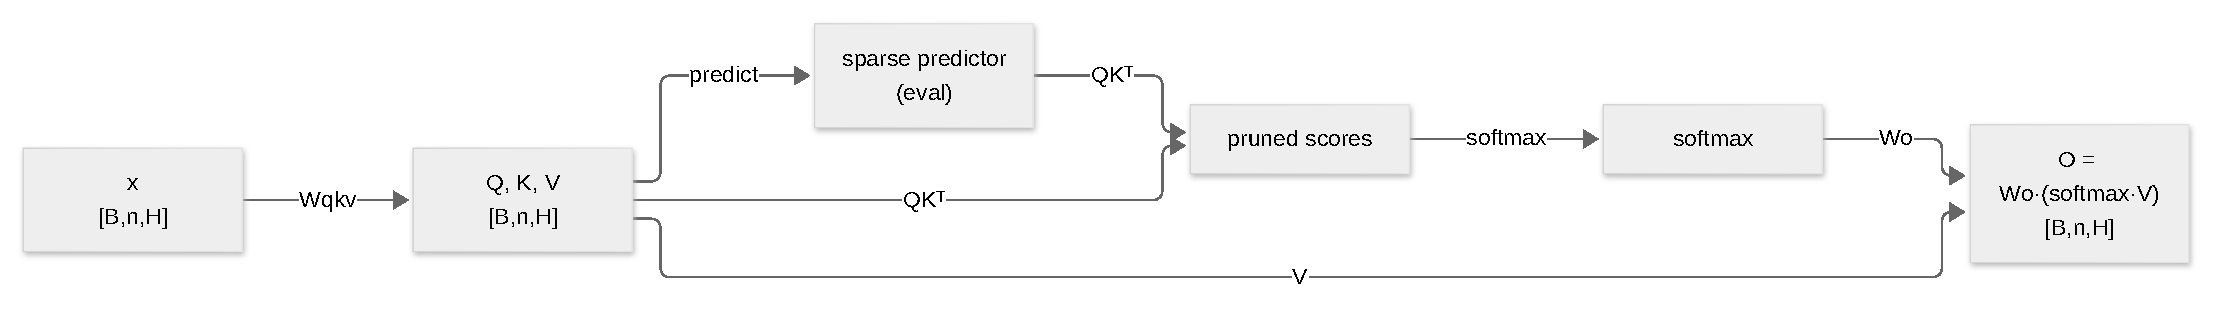
\includegraphics{figures/mixers/sparge.pdf}}
\caption{Dataflow of SpargeAttn: a sparse predictor (evaluation only) prunes key blocks before softmax.}
\label{fig:mixer-sparge}
\end{figure}

\subsubsection{Mathematical Formulation}

SpargeAttn \citep{zhang_spargeattn_2025} is a \textbf{universal training-free method} that predicts which blocks of the attention matrix will contain negligible values and skips computation for those blocks.

\paragraph{Stage 1 --- Sparse prediction}: Compute low-cost proxy importance $\hat{s}_{ij}$ for block $(i,j)$:

\[
\hat{s}_{ij} = f_{\text{pred}}(\mathbf{Q}_i, \mathbf{K}_j; \text{hyperparams}), \quad \text{skip if } \hat{s}_{ij} < \epsilon_1
\]

Common predictors include block-mean similarity or self-similarity statistics.

\paragraph{Stage 2 --- Softmax-aware filtering}: After computing $\tilde{P}_{ij} = \text{softmax}(Q_i K_j^\top/\sqrt{d})$, check if the block's maximum probability is negligible relative to the running softmax maximum:

\[
\text{skip } P_{ij} V_j \quad \text{if} \quad \max(\tilde{P}_{ij}) < e^{m_{\text{old}} - m_{\text{new}}} \cdot \epsilon_2
\]

where $m_{\text{old}}, m_{\text{new}}$ are online softmax running maxima (computed via FlashAttention-style numerics).

\subsubsection{Algorithmic Pseudocode}

\begin{algorithm}[H]
\caption{SpargeAttn: Two-Stage Block-Sparse Filtering}
\begin{algorithmic}[1]
\Require Query blocks $\mathbf{Q}_i$ for $i = 1, \ldots, n_b$, Key blocks $\mathbf{K}_j$ for $j = 1, \ldots, n_b$, Value blocks $\mathbf{V}_j$
\Require Prediction threshold $\epsilon_1$, softmax threshold $\epsilon_2$, block size $b_s$
\Ensure Output $\mathbf{Y}$
\State Initialize: online softmax max $m_{\text{global}} \gets -\infty$
\For{block row $i = 1$ to $n_b$}
    \State Initialize: block row output $\mathbf{Y}_i \gets 0$, local max $m_i \gets -\infty$
    \For{block column $j = 1$ to $n_b$}
        \State \textbf{Stage 1: Sparse Prediction}
        \State Compute proxy importance: $\hat{s}_{ij} \gets f_{\text{pred}}(\mathbf{Q}_i, \mathbf{K}_j)$
        \If{$\hat{s}_{ij} < \epsilon_1$}
            \State \textbf{skip} this block $[i,j]$  \Comment{Early termination}
            \State \textbf{continue} \Comment{Move to next block}
        \EndIf
        \State \textbf{Stage 2: Compute and Filter}
        \State $\tilde{P}_{ij} \gets \text{softmax}(\mathbf{Q}_i \mathbf{K}_j^\top / \sqrt{d})$
        \State $m_{\text{block}} \gets \max(\tilde{P}_{ij})$
        \If{$m_{\text{block}} < e^{m_i - m_{\text{global}}} \cdot \epsilon_2$}
            \State Block contributes negligibly; skip  \Comment{Softmax-aware pruning}
            \State \textbf{continue}
        \EndIf
        \State Update global max: $m_i \gets \max(m_i, m_{\text{block}})$
        \State Accumulate: $\mathbf{Y}_i \gets \mathbf{Y}_i + \tilde{P}_{ij} \mathbf{V}_j$
    \EndFor
    \State $m_{\text{global}} \gets \max(m_{\text{global}}, m_i)$
\EndFor
\Return $\mathbf{Y}$
\end{algorithmic}
\end{algorithm}

\subsubsection{Key Characteristics}

\begin{itemize}[leftmargin=*]
    \item \textbf{Complexity}: Empirical $\mathcal{O}(n^2 \cdot s)$ where $s$ is the fraction of non-skipped blocks (typically 0.2--0.5).
    \item \textbf{Trainable}: No; plug-and-play acceleration for existing models.
    \item \textbf{Universality}: Works on language models, image diffusion models, and video generation.
    \item \textbf{Strength}: 2.5--5$\times$ speedup compared to dense or previous sparse methods; compatible with quantization (SageAttention integration).
    \item \textbf{Limitation}: Speedup depends on inherent sparsity; block-level granularity may miss finer patterns; threshold tuning required per model family.
\end{itemize}

\subsection{MSA (MiniMax Sparse Attention): Blockwise Sparse Attention with Lightweight Index Branch}

\begin{figure}[H]
\centering
\fitfigure{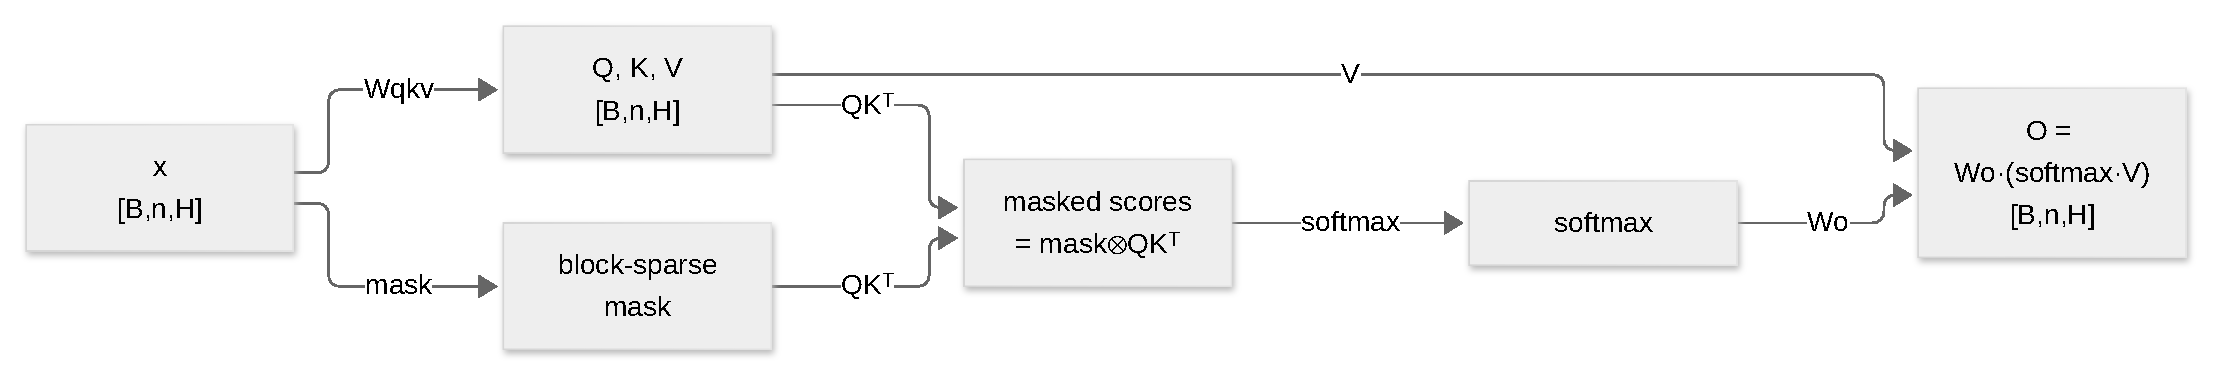
\includegraphics{figures/mixers/msa.pdf}}
\caption{Dataflow of MSA: a block-sparse mask restricts the score matrix before softmax.}
\label{fig:mixer-msa}
\end{figure}

\subsubsection{Mathematical Formulation}

MSA \citep{lai_minimax_2026} is a blockwise sparse attention mechanism built on grouped-query attention (GQA) that combines a lightweight \textbf{Index Branch} for block selection with a \textbf{Main Branch} for exact block-sparse softmax attention over the selected blocks. Let $N$ be the sequence length, $B_k = 128$ the block size, and $k = 16$ the number of blocks selected per query (yielding a fixed per-query budget of $k \cdot B_k = 2048$ tokens regardless of $N$).

\paragraph{Index Branch}: A low-dimensional projection produces index queries $\mathbf{q}_t^{\text{idx}} \in \mathbb{R}^{d_{\text{idx}}}$ and block representatives $\mathbf{r}_b \in \mathbb{R}^{d_{\text{idx}}}$ for each KV block $b$. The index scores per GQA group are:
\[
s_{t,b}^{(g)} = \mathbf{q}_t^{\text{idx},(g)} \cdot \mathbf{r}_b, \qquad \mathcal{I}_t^{(g)} = \mathrm{TopK}\left(\{s_{t,b}^{(g)}\}_{b=1}^{N/B_k},\; k\right)
\]
The index input is \textbf{detached} (stop-gradient), so gradients do not flow back through the indexer's input; the Index Branch is trained instead by a KL alignment loss between its attention distribution and the Main Branch's distribution. Because softmax is order-preserving, the raw index scores feed directly into the top-$k$ operator \emph{without} an explicit softmax (\textbf{exp-free top-$k$}), reducing numerical cost.

\paragraph{Forced local block}: The block containing the query position $t$ is \textbf{always} included in $\mathcal{I}_t^{(g)}$, guaranteeing local context coverage.

\paragraph{Main Branch}: Standard scaled dot-product attention is computed exactly over the union of selected blocks:
\[
\mathbf{o}_t^{(h)} = \mathrm{softmax}\left(\frac{\mathbf{q}_t^{(h)} \mathbf{K}_{\mathcal{I}_t}^{(h)\top}}{\sqrt{d_h}}\right) \mathbf{V}_{\mathcal{I}_t}^{(h)}
\]
where $\mathbf{K}_{\mathcal{I}_t}, \mathbf{V}_{\mathcal{I}_t}$ gather the full-precision key/value tensors of the selected blocks. Selection is performed independently per GQA group, so different query groups within the same layer may attend to different block subsets.

\subsubsection{Algorithmic Pseudocode}

\begin{algorithm}[H]
\caption{MSA: MiniMax Sparse Attention with Index + Main Branches}
\begin{algorithmic}[1]
\Require Query $\mathbf{Q} \in \mathbb{R}^{N \times d}$, Key $\mathbf{K}$, Value $\mathbf{V}$, block size $B_k = 128$, top-$k$ blocks $k = 16$
\Require Index projection $W_{\text{idx}}$ (detached input), block representatives $\{\mathbf{r}_b\}$
\Ensure Output $\mathbf{Y} \in \mathbb{R}^{N \times d}$
\State Compute block reps: $\mathbf{r}_b \gets \mathrm{mean}(\mathbf{K}_{bB_k:(b+1)B_k})$ for $b = 1, \ldots, N/B_k$
\For{query position $t = 1, \ldots, N$}
    \For{each GQA group $g$}
        \State $\mathbf{q}_t^{\text{idx}} \gets \mathrm{sg}(W_{\text{idx}} \mathbf{x}_t)$ \Comment{detached index query}
        \State Compute block scores: $s_b \gets \mathbf{q}_t^{\text{idx}} \cdot \mathbf{r}_b$
        \State Identify local block: $b_{\text{local}} \gets \lfloor t / B_k \rfloor$
        \State $\mathcal{I}_t^{(g)} \gets \mathrm{TopK}(\{s_b\}, k) \cup \{b_{\text{local}}\}$ \Comment{exp-free top-$k$ + forced local}
    \EndFor
    \State Gather selected KV: $\tilde{\mathbf{K}}_t \gets \mathrm{Gather}(\mathbf{K}, \mathcal{I}_t)$, $\tilde{\mathbf{V}}_t \gets \mathrm{Gather}(\mathbf{V}, \mathcal{I}_t)$
    \State Main branch SDPA: $\mathbf{y}_t \gets \mathrm{softmax}(\mathbf{q}_t \tilde{\mathbf{K}}_t^\top / \sqrt{d_h}) \tilde{\mathbf{V}}_t$
\EndFor
\State Add KL alignment loss $\mathcal{L}_{\text{KL}} = \mathrm{KL}(\text{index dist} \,\|\, \text{main dist})$ during training
\Return $\mathbf{Y}$
\end{algorithmic}
\end{algorithm}

\subsubsection{Key Characteristics}

\begin{itemize}[leftmargin=*]
    \item \textbf{Complexity}: Index branch $\mathcal{O}(H_{\text{kv}} \cdot d_{\text{idx}} \cdot N^2)$; Main branch $\mathcal{O}(H_q \cdot d_h \cdot N \cdot k \cdot B_k)$. Per-query budget fixed at $k \cdot B_k = 2048$ tokens regardless of $N$.
    \item \textbf{Trainable}: Yes; end-to-end (the Index Branch is trained via a KL alignment loss, not eval-only).
    \item \textbf{State}: $\mathcal{O}(N)$ KV cache (GQA-sized); no expansion of the recurrent/state dimension.
    \item \textbf{Strength}: Deployed on the 109B MiniMax-M3, MSA achieves a $28.4\times$ per-token attention compute reduction at 1M context, with $14.2\times$ prefill and $7.6\times$ decode speedup on H800 GPUs.
    \item \textbf{Limitation}: Selection granularity is fixed at the block level ($B_k = 128$); the forced local block and per-group independent selection increase engineering complexity and require custom block-sparse kernels.
\end{itemize}

\subsection{SparDA (Sparse Decoupled Attention): Forecast-Guided Lookahead Block Selection}

\begin{figure}[H]
\centering
\fitfigure{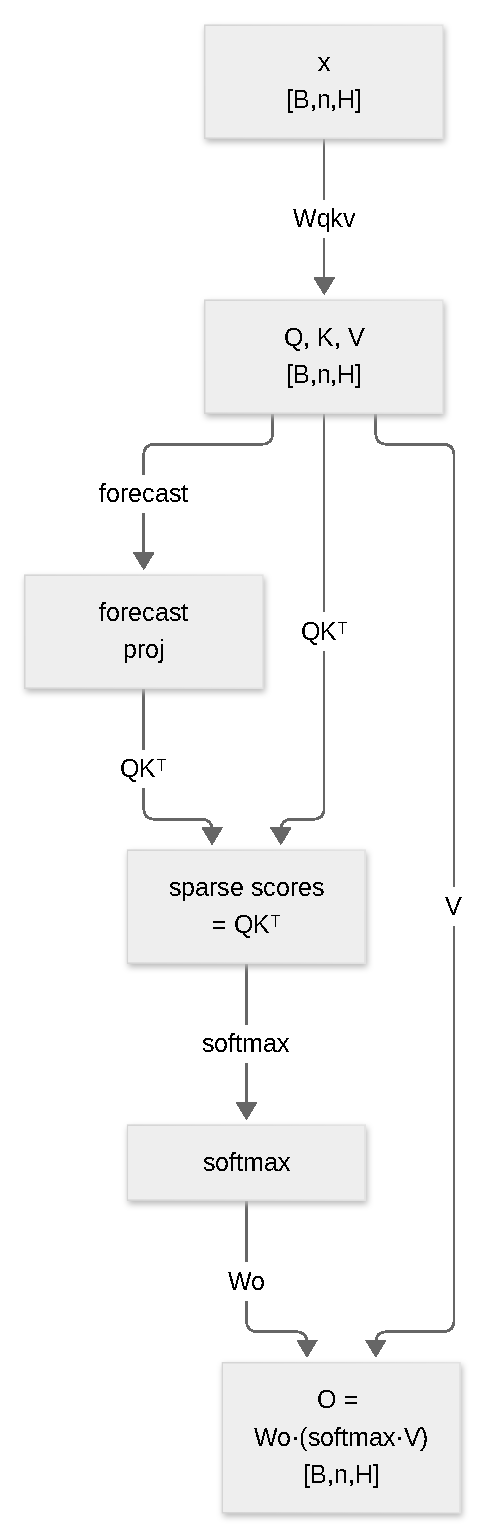
\includegraphics{figures/mixers/sparda.pdf}}
\caption{Dataflow of SparDA: a forecast projection guides lookahead block selection before softmax.}
\label{fig:mixer-sparda}
\end{figure}

\subsubsection{Mathematical Formulation}

SparDA \citep{fu_sparda_2026} introduces a \textbf{decoupled} sparse attention scheme that augments the standard per-layer projections $Q, K, V$ with a fourth projection, the \textbf{Forecast}, which predicts the KV blocks that will be needed by the \emph{next} layer. This lookahead enables overlapping CPU-to-GPU prefetch of the next layer's selected blocks with the current layer's execution, hiding the offload latency that plagues sparse-attention deployments on memory-constrained hardware.

\paragraph{Forecast projection}: For input $\mathbf{x} \in \mathbb{R}^{N \times d}$,
\[
\mathbf{F} = \mathbf{x} \mathbf{W}_F \in \mathbb{R}^{N \times H_{\text{kv}} \times d_f}
\]
with \textbf{one Forecast head per GQA group}, which reduces selection overhead relative to multi-head selectors used by prior work.

\paragraph{Block scoring and selection}: For each query $i$ and KV block $b$ with representative $\mathbf{r}_b$:
\[
S_{i,b} = \mathbf{F}_i \cdot \mathbf{r}_b, \qquad \mathcal{I}_i = \mathrm{TopK}(\{S_{i,b}\}_b, k)
\]
\paragraph{Block-sparse attention}: Standard scaled dot-product attention is then computed over the selected blocks:
\[
\mathbf{o}_i = \mathrm{softmax}\left(\frac{\mathbf{q}_i \mathbf{K}_{\mathcal{I}_i}^\top}{\sqrt{d_h}}\right) \mathbf{V}_{\mathcal{I}_i}
\]
\paragraph{Training}: SparDA adds fewer than $0.5\%$ additional parameters. Only the Forecast projections are trained, by matching the original (frozen) sparse selector's attention distribution---a lightweight distillation that preserves the base model's behaviour while enabling lookahead prefetch.

\subsubsection{Algorithmic Pseudocode}

\begin{algorithm}[H]
\caption{SparDA: Sparse Decoupled Attention with Forecast Prefetch}
\begin{algorithmic}[1]
\Require Input $\mathbf{x} \in \mathbb{R}^{N \times d}$, cached Key/Value blocks, top-$k$ blocks $k$
\Require Projections $W_q, W_k, W_v, W_F$; frozen base selector $\pi_{\text{orig}}$
\Ensure Output $\mathbf{Y}$; prefetched blocks for next layer
\State Compute Forecast: $\mathbf{F} \gets \mathbf{x} \mathbf{W}_F$ \Comment{one head per GQA group}
\For{query $i = 1, \ldots, N$}
    \State Compute block scores: $S_{i,b} \gets \mathbf{F}_i \cdot \mathbf{r}_b$ for each block $b$
    \State Select: $\mathcal{I}_i \gets \mathrm{TopK}(\{S_{i,b}\}, k)$
    \State \textbf{Prefetch} $\mathbf{K}_{\mathcal{I}_i}, \mathbf{V}_{\mathcal{I}_i}$ from CPU to GPU for the \emph{next} layer \Comment{overlaps with current layer}
\EndFor
\State Compute block-sparse SDPA over current-layer selected blocks: $\mathbf{Y} \gets \mathrm{BlockSparseSDPA}(\mathbf{Q}, \mathbf{K}, \mathbf{V}, \{\mathcal{I}_i\})$
\State Training loss: $\mathcal{L} \gets \mathrm{KL}(\text{Forecast dist} \,\|\, \pi_{\text{orig}})$ \Comment{only $W_F$ is updated}
\Return $\mathbf{Y}$
\end{algorithmic}
\end{algorithm}

\subsubsection{Key Characteristics}

\begin{itemize}[leftmargin=*]
    \item \textbf{Complexity}: Forecast $\mathcal{O}(H_{\text{kv}} \cdot d_f \cdot N \cdot N_{\text{blocks}})$; Main attention $\mathcal{O}(H_q \cdot d_h \cdot N \cdot k \cdot B_k)$.
    \item \textbf{Trainable}: Yes; only the Forecast projections are trained ($<0.5\%$ extra parameters).
    \item \textbf{Strength}: On two 8B sparse-pretrained models, SparDA achieves up to $1.25\times$ prefill and $1.7\times$ decode speedup over the sparse-attention offload baseline, and up to $5.3\times$ decode throughput versus a non-offload sparse baseline.
    \item \textbf{Limitation}: Requires a CPU--GPU offload pipeline and a frozen base selector; the lookahead benefit is contingent on next-layer block demand being predictable from the current Forecast.
\end{itemize}

\subsection{Design Space and Selection Criteria}

The seven sparse attention methods occupy complementary positions in a multidimensional design space:

\begin{itemize}[leftmargin=*]
    \item \textbf{Geometric/fixed patterns} (Sparse Transformer, Longformer): Simple to implement and analyze, but patterns do not adapt to content.
    \item \textbf{Learned selection} (SparseK, NSA): Enable adaptation through trainable selection networks, at the cost of higher implementation complexity.
    \item \textbf{Training-free acceleration} (FASA, SpargeAttn): Enable drop-in speedup of existing models without retraining, suited for deployed systems.
    \item \textbf{Theoretical guarantees} (BigBird): Provide formal proofs of expressive completeness, important for understanding safety margins.
\end{itemize}

\textbf{Selection guidance:}
\begin{enumerate}[leftmargin=*]
    \item \textbf{New model training} where resources permit: NSA or SparseK for maximal inference speedup; BigBird for theoretical assurance.
    \item \textbf{Long-context document understanding}: Longformer or FASA for practical simplicity; NSA for extreme scale.
    \item \textbf{Accelerating existing models}: FASA for RoPE-based LLMs; SpargeAttn for any architecture.
    \item \textbf{Constrained environments}: Sparse Transformer for simplicity and proven efficiency at moderate scale.
\end{enumerate}


\section{Gated Attention Families---Complete Literature Analysis}
\label{sec:annex-gated}

\subsection{Executive Summary: Gating for Memory Control}

The emerging field of \emph{gated attention mechanisms} addresses a fundamental challenge in sequence modeling: how should information be retained, forgotten, and updated as the model processes new tokens? Traditional additive recurrent states accumulate all information without erasure, leading to memory saturation and inability to adapt to changing context. Softmax attention provides full expressiveness but uses $\mathcal{O}(Ld)$ KV cache during inference, limiting context window size. Gated mechanisms provide a middle ground: selective control over information survival.

The unifying principle across gated architectures is that gating controls \textit{what information survives}. Gates operate at three distinct levels:
\begin{enumerate}[leftmargin=*]
    \item \textbf{Recurrent state decay} (GLA, HGRN2): Multiplicative gates on the memory matrix $S_t$ control how much previous state persists into the next step.
    \item \textbf{Write strength in recurrent updates} (DeltaNet, Gated DeltaNet, Gated DeltaNet-2): Gates control the magnitude and channel-wise direction of new information written into memory.
    \item \textbf{Softmax logit biasing} (FoX): Gates inject token-level recency bias into attention logit computation.
    \item \textbf{Post-attention sparsity} (Gated Softmax): Gates selectively scale SDPA output channels.
\end{enumerate}

This appendix synthesizes eight major gated-attention architectures published 2023--2026, analyzing their mathematical foundations, hardware efficiency characteristics, and empirical trade-offs.

\subsection{1. Gated Linear Attention (GLA)}

\begin{figure}[H]
\centering
\fitfigure{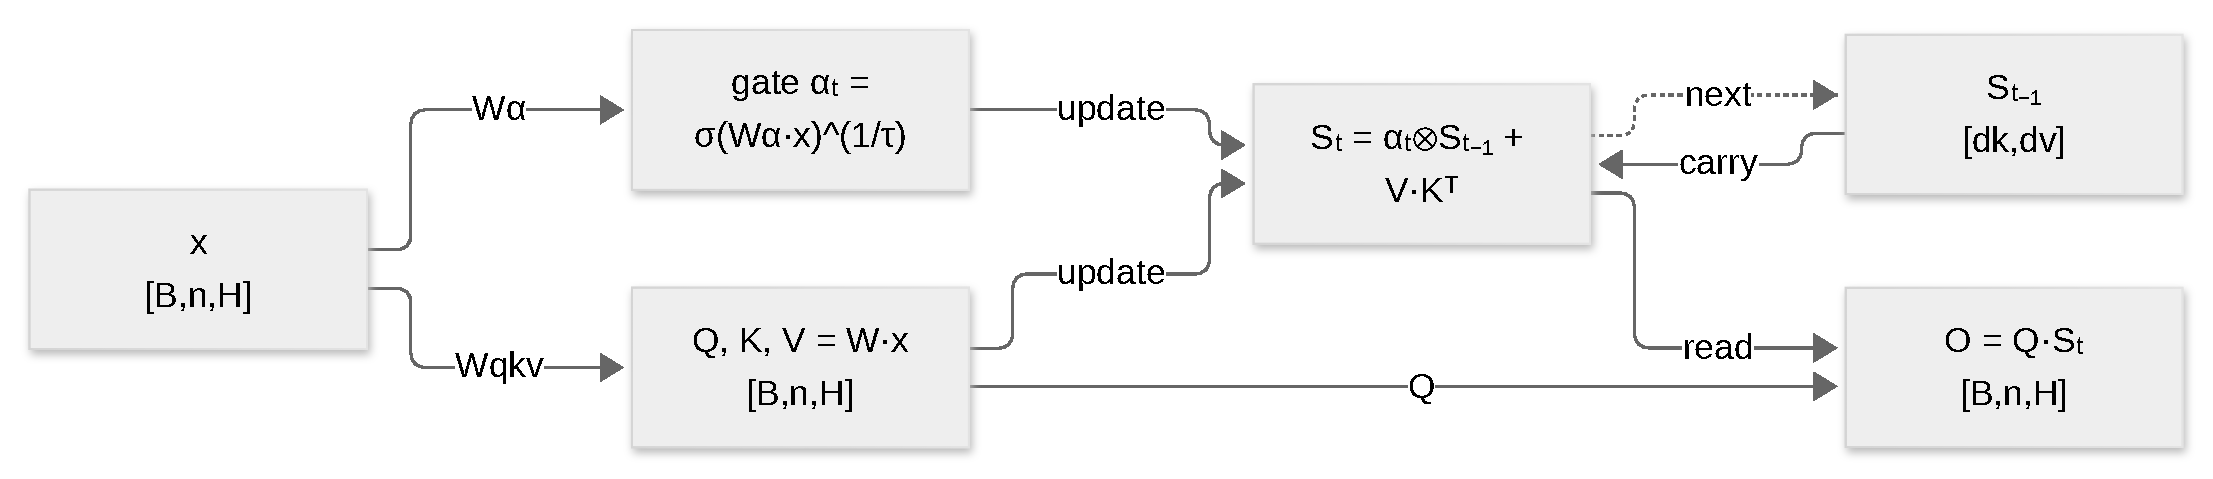
\includegraphics{figures/mixers/gla.pdf}}
\caption{Dataflow of GLA: a sigmoid gate decays the recurrent state before the key/value outer product is added.}
\label{fig:mixer-gla}
\end{figure}

\subsubsection{Mathematical Foundation}

Gated Linear Attention \citep{yang_gla_2023} augments vanilla linear attention (which uses a matrix-valued recurrent state) with data-dependent multiplicative decay. Standard linear attention reformulates the traditional softmax mechanism as a recurrence over hidden states:
\[
\mathbf{S}_t = \mathbf{S}_{t-1} + \mathbf{v}_t \mathbf{k}_t^\top, \quad \mathbf{o}_t = \mathbf{S}_t \mathbf{q}_t
\]
where state $\mathbf{S}_t \in \mathbb{R}^{d_v \times d_k}$ accumulates outer products. This purely additive formulation suffers from ``memory overload'': information accumulates monotonically and cannot be erased, degrading performance on tasks requiring context selection.

GLA introduces a data-dependent \textbf{diagonal gating matrix} $\mathbf{G}_t \in [0,1]^{d_k \times d_k}$:
\[
\mathbf{S}_t = \mathbf{G}_t \odot \mathbf{S}_{t-1} + \mathbf{v}_t \mathbf{k}_t^\top, \quad \mathbf{o}_t = \mathbf{S}_t \mathbf{q}_t
\]
The gate $\mathbf{G}_t$ is parameterized with an outer-product structure:
\[
\mathbf{G}_t = \mathbf{1} \boldsymbol{\alpha}_t^\top, \quad \boldsymbol{\alpha}_t = \text{logsigmoid}\left(\mathbf{W}_{gk} \mathbf{x}_t\right) / c
\]
where $\mathbf{W}_{gk}$ is a low-rank projection ($\mathbb{R}^{d \to d_k}$) and $c \approx 16$ is a normalizer. The logsigmoid activation maps $\alpha_t \in \mathbb{R}$ to approximately $[-1/2, 0]$, and division by $c$ further contracts this to near-identity for initialization. The resulting gate $G_t = 1 + \alpha_t \approx 1$ near initialization, then learns to decay $(\alpha_t \to -\infty)$ historical information.

\begin{algorithm}[H]
\caption{Gated Linear Attention (Recurrent Form)}
\begin{algorithmic}[1]
\Require Input $\mathbf{x}_t$; prior state $\mathbf{S}_{t-1}$
\Require Projections: $W_q, W_k, W_v$ (standard); $W_{gk}$ (gate projection)
\Ensure Output $\mathbf{o}_t$ and updated state $\mathbf{S}_t$
\State $\mathbf{q}_t \gets W_q \mathbf{x}_t$
\State $\mathbf{k}_t \gets W_k \mathbf{x}_t$
\State $\mathbf{v}_t \gets W_v \mathbf{x}_t$
\State Compute gate: $\boldsymbol{\alpha}_t \gets \text{logsigmoid}(W_{gk} \mathbf{x}_t) / 16$ \Comment{Per-key-dim decay}
\State Apply outer-product gating: $\mathbf{G}_t \gets \mathbf{1} \boldsymbol{\alpha}_t^\top$  \Comment{diagonal outer product}
\State Decay previous state: $\mathbf{S}_t^\text{decay} \gets \mathbf{G}_t \odot \mathbf{S}_{t-1}$ \Comment{element-wise product}
\State Add new association: $\mathbf{S}_t \gets \mathbf{S}_t^\text{decay} + \mathbf{v}_t \mathbf{k}_t^\top$
\State Retrieve via query: $\mathbf{o}_t^\text{raw} \gets \mathbf{S}_t \mathbf{q}_t$
\State Apply output gate: $\mathbf{o}_t \gets \text{GroupNorm}(\mathbf{o}_t^\text{raw}) \otimes \text{SiLU}(W_g \mathbf{x}_t)$
\Return $\mathbf{o}_t$, $\mathbf{S}_t$
\end{algorithmic}
\end{algorithm}

\subsubsection{Hardware-Efficient Training}

For parallel training, GLA uses a chunkwise block-wise algorithm that groups tokens into chunks $C$ and computes recurrent transitions in parallel:
\[
\mathbf{O}_{[t]} = \overleftarrow{\mathbf{Q}}_{[t]} \mathbf{S}_{[t]}^\top + \left(\mathbf{Q}_{[t]} \mathbf{K}_{[t]}^\top \odot \mathbf{\Gamma}_{[t]}\right) \mathbf{V}_{[t]}
\]
where $\overleftarrow{\mathbf{Q}}_{[t]}$ are attending to the state at the chunk boundary (lookback), and $\mathbf{\Gamma}_{[t]}$ is the causal mask with decay-aware scaling:
\[
\mathbf{\Gamma}_{[t],ij} = \begin{cases} \prod_{l=j}^{i-1} \alpha_l & \text{if } i > j \text{ (lookback)} \\ \prod_{l=1}^{i-j} \alpha_l & \text{if } i \le j \text{ (in-chunk)} \end{cases}
\]
This design maximizes matmul operations susceptible to tensor-core acceleration, achieving sub-quadratic total complexity $\mathcal{O}(nLd^2/C)$ where $L$ is the number of attention heads and $C$ is chunk size.

\subsubsection{Strengths and Limitations}

\begin{table}[H]
\centering
\small
\begin{tabularx}{0.95\linewidth}{Xp{4cm}p{4cm}}
\toprule
\textbf{Aspect} & \textbf{Strengths} & \textbf{Limitations} \\
\midrule
Computational efficiency & Sub-quadratic training via chunkwise parallelism. Constant-memory inference $O(d^2)$. & Requires custom CUDA/Triton kernels; not available in all frameworks. \\
Context generalization & Extends 2K-token training to 20K+ tokens with negligible perplexity degradation. & Still underperforms softmax on retrieval-heavy benchmarks (needle-in-haystack). \\
Selectivity & Per-key-dimension data-dependent decay. & Gate structure limits per-key-value selectivity; no direct control over which specific associations to erase. \\
\bottomrule
\end{tabularx}
\end{table}

\subsection{2. DeltaNet: Error-Correcting Linear Attention}

\begin{figure}[H]
\centering
\fitfigure{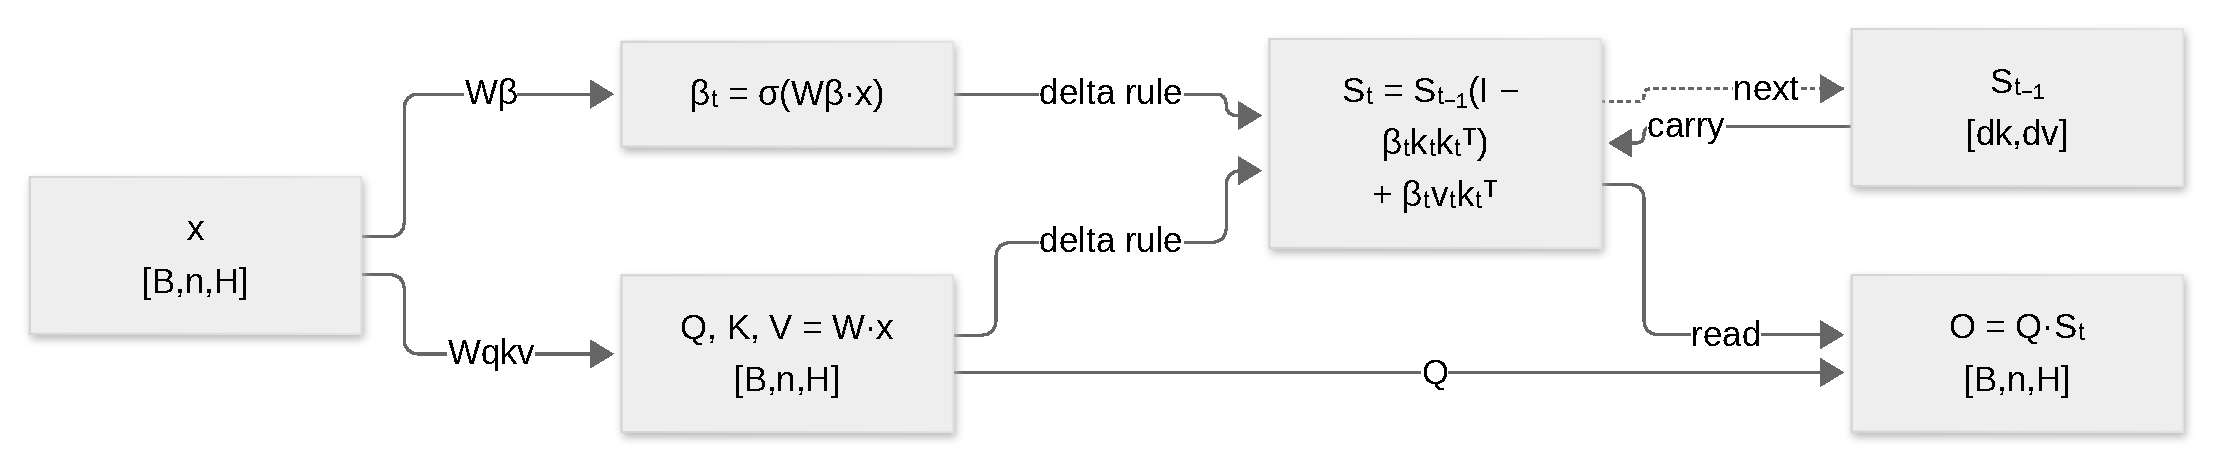
\includegraphics{figures/mixers/deltanet.pdf}}
\caption{Dataflow of DeltaNet: the beta gate applies an error-correcting delta rule to the recurrent state.}
\label{fig:mixer-deltanet}
\end{figure}

\subsubsection{Mathematical Foundation}

DeltaNet \citep{yang_deltanet_2024} applies a classical \textbf{delta learning rule} to linear attention state updates. Instead of additive accumulation, DeltaNet computes the difference between the predicted value (retrieved from memory) and the target value, then performs an error-correcting update:
\[
\mathbf{S}_t = \mathbf{S}_{t-1}(\mathbf{I} - \beta_t \mathbf{k}_t \mathbf{k}_t^\top) + \beta_t \mathbf{v}_t \mathbf{k}_t^\top
\]
where $\beta_t \in (0,1)$ is a data-dependent \textbf{writing strength} scalar. This update can be decomposed as an erase-write operation:
\[
\mathbf{v}_t^\text{old} = \mathbf{S}_{t-1} \mathbf{k}_t \quad \text{(current prediction)}, \quad
\mathbf{v}_t^\text{updated} = \beta_t \mathbf{v}_t + (1-\beta_t)\mathbf{v}_t^\text{old} \quad \text{(blend old/new)}
\]
so that:
\[
\mathbf{S}_t = \mathbf{S}_{t-1} - \mathbf{v}_t^\text{old}\mathbf{k}_t^\top + \mathbf{v}_t^\text{updated}\mathbf{k}_t^\top
\]
The key insight is that this update rule minimizes an online MSE loss at each timestep:
\[
\mathcal{L}_t(\mathbf{S}) = \tfrac{1}{2}\|\mathbf{S}\mathbf{k}_t - \mathbf{v}_t\|^2 \Rightarrow \nabla_{\mathbf{S}} \mathcal{L}_t = (\mathbf{S}\mathbf{k}_t - \mathbf{v}_t)\mathbf{k}_t^\top
\]
One step of SGD with learning rate $\beta_t$ yields the delta rule update. This connection to test-time training (TTT) provides theoretical grounding: DeltaNet is directly optimizing for value prediction at inference time.

\subsubsection{Efficient Parallel Training}

DeltaNet's transition matrix $\mathbf{I} - \beta_t \mathbf{k}_t \mathbf{k}_t^\top$ is a generalized Householder matrix (rank-1 update to identity). For chunkwise training, DeltaNet uses the \textbf{WY representation}, which represents the product of $m$ such rank-1 updates compactly:
\[
\prod_{i=1}^{m} (\mathbf{I} - \beta_i \mathbf{k}_i \mathbf{k}_i^\top) = \mathbf{I} - \mathbf{W}\mathbf{Y}^\top
\]
where $\mathbf{W}, \mathbf{Y} \in \mathbb{R}^{d \times m}$ are constructed recursively. This factorization enables matmul-rich parallelism without materializing the full product, keeping chunkwise training efficient.

\begin{algorithm}[H]
\caption{DeltaNet State Update with WY Representation}
\begin{algorithmic}[1]
\Require Input chunk $\mathbf{X}_{[t]}$; prior state $\mathbf{S}_{t-1}$
\Require L2-normalized queries $\hat{\mathbf{Q}}_t$, keys $\hat{\mathbf{K}}_t$, values $\mathbf{V}_t$
\Ensure Output $\mathbf{O}_{[t]}$ and updated state $\mathbf{S}_t$
\State \textbf{Chunkwise phase:}
\For{position $i = 1$ to chunk\_size}
    \State Normalize: $\hat{\mathbf{k}}_i \gets \hat{\mathbf{K}}_t[i] / \|\hat{\mathbf{K}}_t[i]\|$, $\hat{\mathbf{q}}_i \gets \hat{\mathbf{Q}}_t[i] / \|\hat{\mathbf{Q}}_t[i]\|$
    \State Compute write strength: $\beta_i \gets \text{sigmoid}(W_\beta \mathbf{x}_i)$
    \State Prediction: $\hat{\mathbf{v}}^\text{pred} \gets \mathbf{S}_{i-1}^\text{in-chunk} \hat{\mathbf{k}}_i$
    \State Error-aware blend: $\mathbf{v}_i^\text{update} \gets \beta_i(\mathbf{v}_i - \hat{\mathbf{v}}^\text{pred})$
    \State Erase-write: $\mathbf{S}_i^\text{in-chunk} \gets \mathbf{S}_{i-1}^\text{in-chunk} - \hat{\mathbf{v}}^\text{pred}\hat{\mathbf{k}}_i^\top + (\beta_i \mathbf{v}_i + (1-\beta_i)\hat{\mathbf{v}}^\text{pred})\hat{\mathbf{k}}_i^\top$
    \State Output: $\mathbf{o}_i \gets \mathbf{S}_i^\text{in-chunk} \hat{\mathbf{q}}_i$
\EndFor
\State \textbf{Inter-chunk phase:} Use WY representation of transition products
\Return $\mathbf{O}_{[t]}$, $\mathbf{S}_{t}$
\end{algorithmic}
\end{algorithm}

\subsubsection{Strengths and Limitations}

\begin{table}[H]
\centering
\small
\begin{tabularx}{0.95\linewidth}{Xp{4cm}p{4cm}}
\toprule
\textbf{Aspect} & \textbf{Strengths} & \textbf{Limitations} \\
\midrule
Associative recall & Perfect recall on Multi-Query Associative Recall (MQAR) benchmark; error-correcting semantics naturally fit retrieval patterns. & Without global forgetting, memory still crowds over extreme sequence lengths; requires periodic reset mechanisms for unbounded context. \\
Theory & Grounded in online MSE optimization; clear connection to test-time training paradigm. & Requires L2-normalized keys for numerical stability; double-width normalization adds overhead. \\
Throughput & WY representation enables efficient chunkwise training. & Slightly slower than Mamba2 per-token due to richer transition matrices (rank-1 instead of diagonal). \\
\bottomrule
\end{tabularx}
\end{table}

\subsection{3. Gated DeltaNet: Synthesis of Gating and Error Correction}

\begin{figure}[H]
\centering
\fitfigure{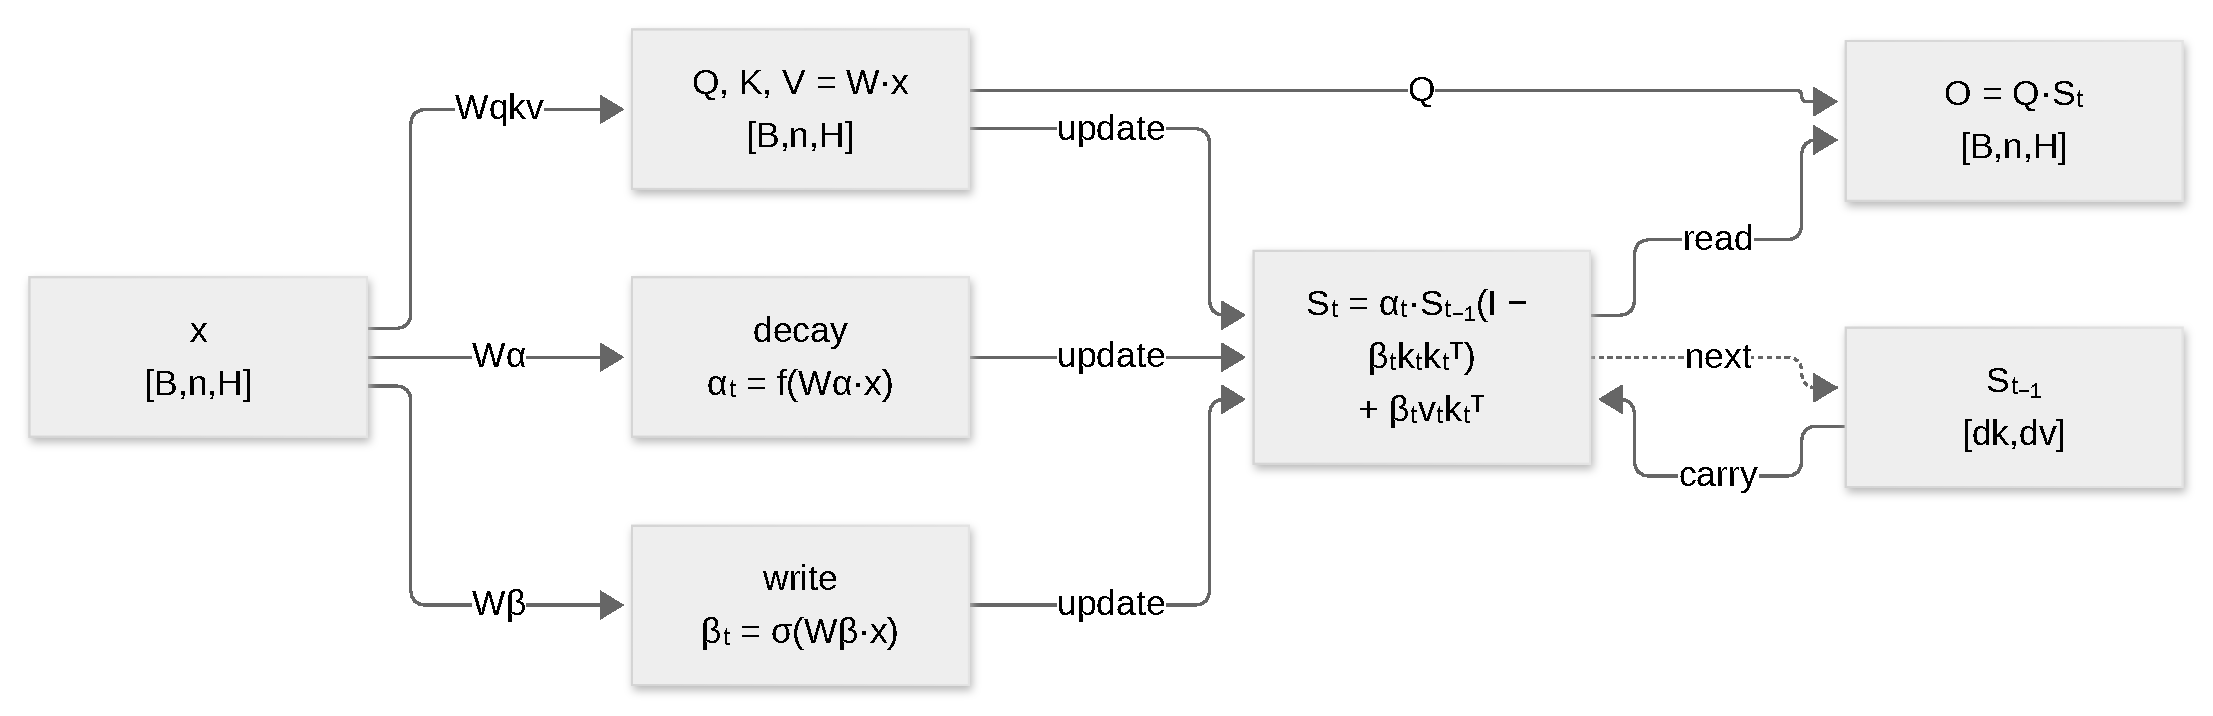
\includegraphics{figures/mixers/gated-deltanet.pdf}}
\caption{Dataflow of Gated DeltaNet: decay and write gates modulate the delta-rule state update.}
\label{fig:mixer-gated-deltanet}
\end{figure}

\subsubsection{Mathematical Foundation}

Gated DeltaNet \citep{yang_gated_deltanet_2024} synthesizes the strengths of GLA and DeltaNet by combining a \textbf{decay gate} $\alpha_t$ (from GLA) with the \textbf{writing strength gate} $\beta_t$ (from DeltaNet):
\[
\mathbf{S}_t = \mathbf{S}_{t-1}\left(\alpha_t (\mathbf{I} - \beta_t \mathbf{k}_t \mathbf{k}_t^\top)\right) + \beta_t \mathbf{v}_t \mathbf{k}_t^\top
\]
Rewriting for clarity:
\[
\mathbf{S}_t = \alpha_t \mathbf{S}_{t-1}(\mathbf{I} - \beta_t \mathbf{k}_t \mathbf{k}_t^\top) + \beta_t \mathbf{v}_t \mathbf{k}_t^\top
\]
The two gates are complementary:
\begin{itemize}[leftmargin=*]
    \item $\alpha_t \to 0$ rapidly erases historical state: $\mathbf{S}_t \approx \beta_t \mathbf{v}_t \mathbf{k}_t^\top$ (context reset).
    \item $\alpha_t \to 1$ recovers pure delta-rule behavior: $\mathbf{S}_t \approx \mathbf{S}_{t-1}(\mathbf{I} - \beta_t \mathbf{k}_t \mathbf{k}_t^\top) + \beta_t \mathbf{v}_t \mathbf{k}_t^\top$ (targeted updates).
    \item $\beta_t \to 0$ skips writing but decays: $\mathbf{S}_t \approx \alpha_t \mathbf{S}_{t-1}$ (pure forgetting).
    \item $\beta_t \to 1$ replaces memory aggressively: $\mathbf{S}_t \approx \alpha_t \mathbf{S}_{t-1} + \mathbf{v}_t \mathbf{k}_t^\top$ (replacement).
\end{itemize}

From an online learning perspective, Gated DeltaNet corresponds to:
\[
\min_{\mathbf{S}_t} \|\mathbf{S}_t - \alpha_t \mathbf{S}_{t-1}\|_F^2 - 2\langle \mathbf{S}_t \mathbf{k}_t, \beta_t(\mathbf{v}_t - \alpha_t \mathbf{S}_{t-1} \mathbf{k}_t)\rangle
\]
which introduces an adaptive weight decay $\alpha_t$ into an SGD-like update---analogous to decoupled weight decay in deep learning optimization.

\begin{algorithm}[H]
\caption{Gated DeltaNet Parallel Chunkwise Forward}
\begin{algorithmic}[1]
\Require Input chunk  $\mathbf{X}_{[i]}$; prior state $\mathbf{S}_{i-1}$; chunk size $C$
\Require Projections: $W_q, W_k, W_v, W_\alpha, W_\beta$
\Ensure Output $\mathbf{O}_{[i]}$ and state $\mathbf{S}_i$
\State \textbf{In-chunk computation:}
\For{$j = 1$ to $C$}
    \State $\mathbf{q}_j \gets W_q \mathbf{x}_j$, $\mathbf{k}_j \gets W_k \mathbf{x}_j$, $\mathbf{v}_j \gets W_v \mathbf{x}_j$
    \State $\alpha_j \gets \text{sigmoid}(W_\alpha \mathbf{x}_j)$, $\beta_j \gets \text{sigmoid}(W_\beta \mathbf{x}_j)$
    \State Apply combined gate: $\mathbf{S}_j \gets \alpha_j \mathbf{S}_{j-1}(\mathbf{I} - \beta_j \mathbf{k}_j \mathbf{k}_j^\top) + \beta_j \mathbf{v}_j \mathbf{k}_j^\top$
    \State $\mathbf{o}_j \gets \mathbf{S}_j \mathbf{q}_j$
\EndFor
\State \textbf{Inter-chunk recurrence:}
\State $\mathbf{S}_i \gets \mathbf{S}_C$ from in-chunk; propagate across chunks via cumulative $\prod \alpha$ masks
\State \textbf{Output gating:} $\mathbf{O}_{[i]} \gets \text{GroupNorm}(\mathbf{O}^\text{raw}) \otimes \text{SiLU}(W_g \mathbf{X}_{[i]})$
\Return $\mathbf{O}_{[i]}$, $\mathbf{S}_i$
\end{algorithmic}
\end{algorithm}

\subsubsection{Empirical Performance and Trade-offs}

Gated DeltaNet has been integrated into Alibaba's Qwen3-Next and Qwen3.5 production models. Empirically:
\[
\begin{array}{l|cccc}
\textbf{Task} & \textbf{Gated DeltaNet} & \textbf{Mamba2} & \textbf{DeltaNet} & \textbf{GLA} \\
\hline
\text{Language Modeling} & \mathbf{1.0\times} & 1.08\times & 1.05\times & 1.12\times \\
\text{Associative Recall} & \mathbf{1.0\times} & --(no perfect) & \mathbf{1.0\times} & 0.75 \\
\text{Length Extrapolation} & \mathbf{1.0\times} & 0.98\times & 0.96\times & 0.94\times \\
\text{Throughput (tokens/sec)} & 0.85\times & \mathbf{1.0\times} & 0.82\times & 0.88\times
\end{array}
\]
Gated DeltaNet achieves the best balance across diverse tasks at the cost of slightly reduced throughput due to richer transition matrices.

\subsection{4. HGRN2: Hierarchical Gating with Outer-Product Expansion}

\begin{figure}[H]
\centering
\fitfigure{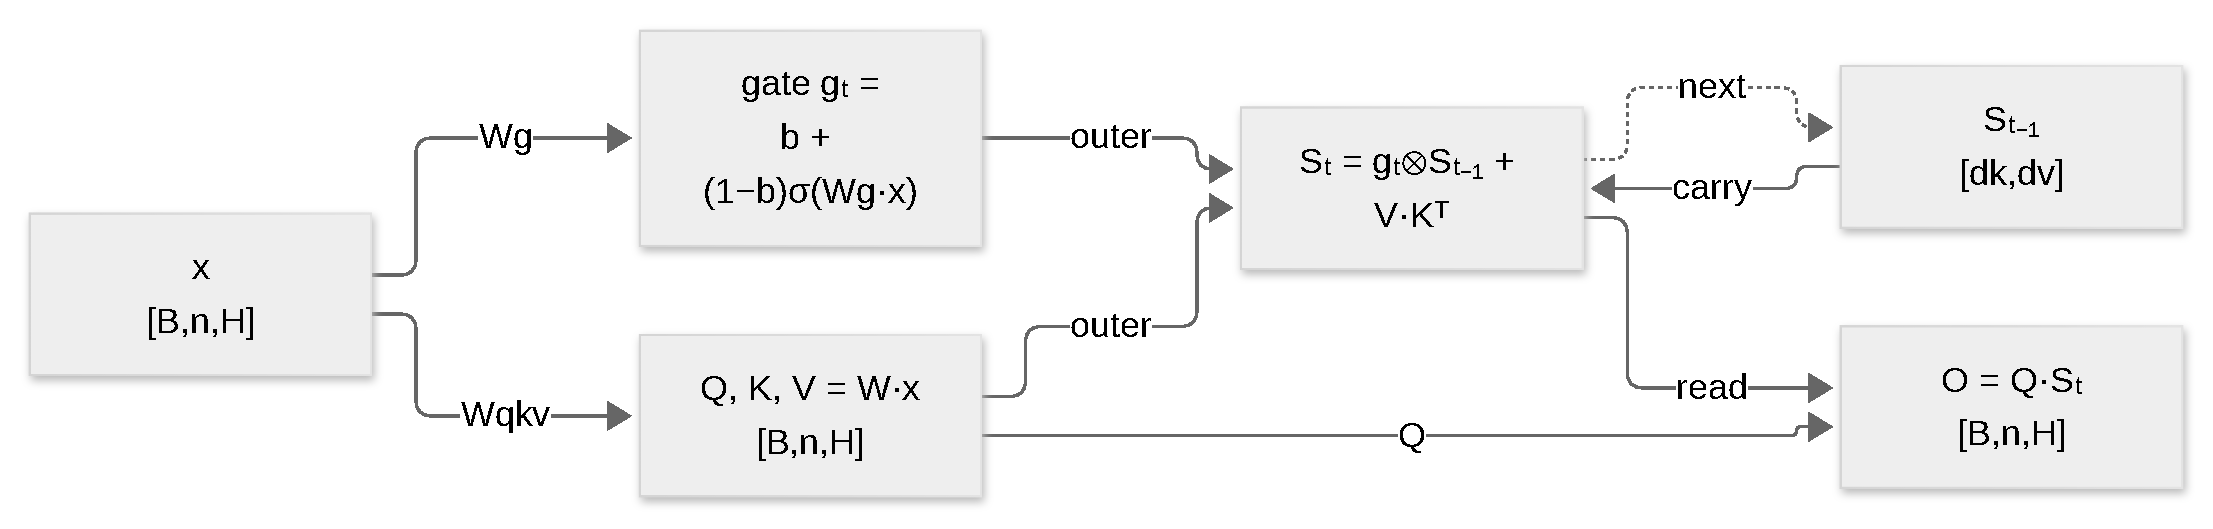
\includegraphics{figures/mixers/hgrn2.pdf}}
\caption{Dataflow of HGRN2: a hierarchical gate mixes the carried state with the key/value outer product.}
\label{fig:mixer-hgrn2}
\end{figure}

\subsubsection{Mathematical Foundation}

HGRN2 \citep{qin_hgrn2_2024} uses an outer-product-based state expansion with \textbf{hierarchically lower-bounded forget gates}. The state update is:
\[
\mathbf{S}_t = \text{diag}(\mathbf{g}_t) \cdot \mathbf{S}_{t-1} + \mathbf{v}_t \mathbf{k}_t^\top, \quad \mathbf{o}_t = \mathbf{S}_t \mathbf{q}_t
\]
where $\mathbf{g}_t \in [b_\ell, 1]^d$ is a lower-bounded forget gate for layer $\ell$. The bounds satisfy:
\[
0 \le b_{\ell_{\text{shallow}}} < b_{\ell_{\text{middle}}} < b_{\ell_{\text{deep}}} \le 1
\]
i.e., bounds increase (become less restrictive) in the deeper layers. The gate itself is computed as:
\[
\mathbf{g}_t = b_\ell + (1 - b_\ell) \cdot \sigma(W_g \mathbf{x}_t)
\]
where $\sigma$ is sigmoid. When $W_g$ outputs weakly negative logits, $\mathbf{g}_t \approx b_\ell$ (forced retention at shallow layers). When outputs are strongly positive, $\mathbf{g}_t \approx 1$ (memory refresh at any layer).

The hierarchical structure encourages different layers to specialize to different timescales: shallow layers model local dependencies (high retention due to binding $b_\ell$), while deeper layers capture long-range structure (flexible gating with high upper bound).

\begin{algorithm}[H]
\caption{HGRN2 Forward with Hierarchical Bounds}
\begin{algorithmic}[1]
\Require Input $\mathbf{x}_t$; prior state $\mathbf{S}_{t-1}$; layer index $\ell \in [0, L-1]$
\Require Non-decreasing bounds: $0 \le b_0 < b_1 < \cdots < b_{L-1} \le 1$
\Ensure Output $\mathbf{o}_t$ and state $\mathbf{S}_t$
\State Layer-specific retain bound: $b \gets b_\ell$
\State Project: $\mathbf{q}_t \gets W_q \mathbf{x}_t$, $\mathbf{k}_t \gets W_k \mathbf{x}_t$, $\mathbf{v}_t \gets W_v \mathbf{x}_t$
\State Compute forget gate with binding: $\mathbf{g}_t \gets b + (1-b) \cdot \sigma(W_g \mathbf{x}_t)$ \Comment{Constrained to $[b, 1]$}
\State Diagonal multiplication (vectorized): $\mathbf{S}_t \gets \mathbf{S}_{t-1} \circ \text{diag}(\mathbf{g}_t) + \mathbf{v}_t \mathbf{k}_t^\top$
\State Retrieve: $\mathbf{o}_t \gets \mathbf{S}_t \mathbf{q}_t$
\State Optional normalization: $\mathbf{o}_t \gets \text{RMSNorm}(\mathbf{o}_t)$
\Return $\mathbf{o}_t$, $\mathbf{S}_t$
\end{algorithmic}
\end{algorithm}

\subsubsection{Scaling and Empirical Results}

At 3B scale on 100B tokens, HGRN2 slightly outperforms Mamba2 and LLaMA-architecture Transformers on language modeling. The hierarchical gating provides multi-scale temporal modeling without explicit layer-wise architectural variants. However, vector-valued diagonal gating (as opposed to element-wise selection) provides less per-item flexibility than delta-rule variants.

\subsection{5. Forgetting Transformer (FoX): Gating in Softmax Logit Space}

\begin{figure}[H]
\centering
\fitfigure{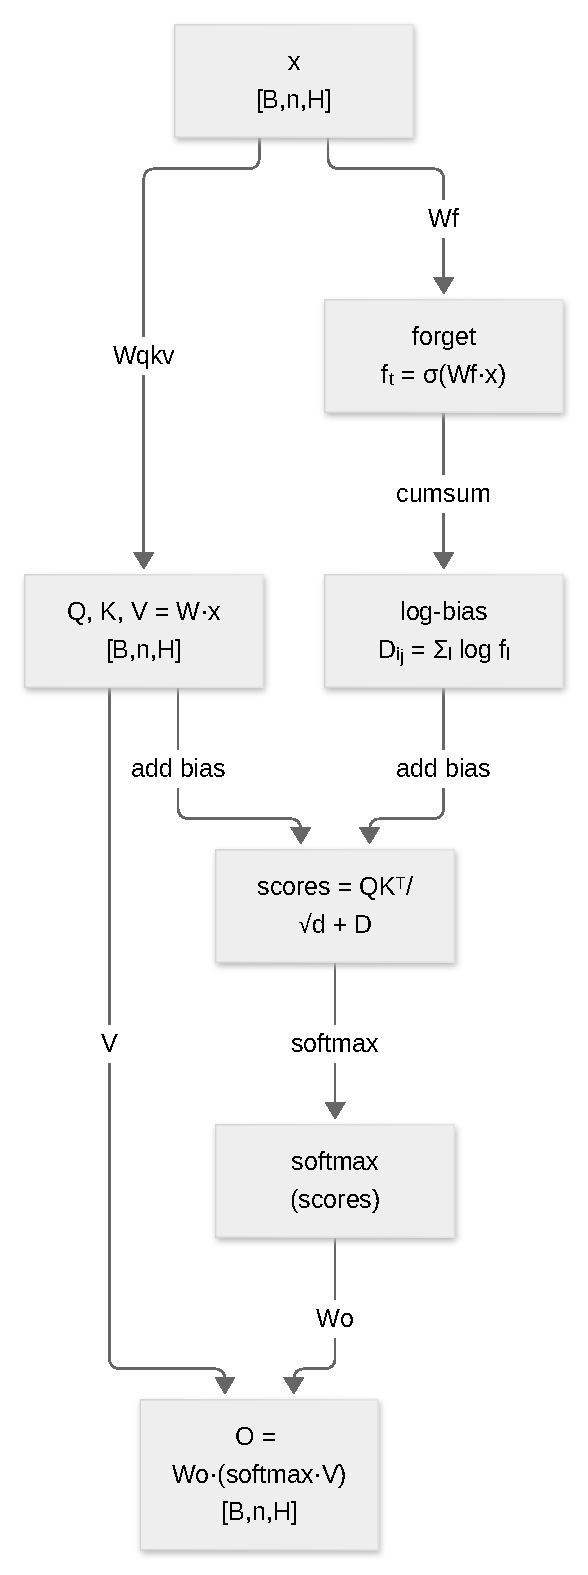
\includegraphics{figures/mixers/fox.pdf}}
\caption{Dataflow of FoX: a learned forget gate becomes an additive log-bias on the score matrix.}
\label{fig:mixer-fox}
\end{figure}

\subsubsection{Mathematical Foundation}

Forgetting Transformer (FoX), proposed by Lin et al.~\citep{lin_forgetting_transformer_2025}, embeds a forget gate directly into softmax attention logits. Rather than replacing softmax with linear recurrence, FoX preserves full softmax expressiveness while adding recency control through a data-dependent logit bias.

For each token position $t$ and all keys $j \le t$, compute a scalar forget gate:
\[
f_t = \sigma(w_f^\top \mathbf{x}_t + b_f)
\]
The logit bias at position $(i,j)$ is the cumulative log-forget product:
\[
d_{ij} = \sum_{l=j+1}^{i} \log f_l = \log \prod_{l=j+1}^{i} f_l
\]
The full attention output becomes:
\[
\mathbf{O} = \text{softmax}\left(\frac{\mathbf{Q}\mathbf{K}^\top}{\sqrt{d_k}} + \mathbf{D}\right) \mathbf{V}
\]
where $\mathbf{D}_{ij} = d_{ij}$. Equivalently:
\[
\text{Attention}(i,j) = \frac{\exp(\mathbf{q}_i^\top \mathbf{k}_j / \sqrt{d_k} + d_{ij})}{\sum_{j'=1}^{i} \exp(\mathbf{q}_i^\top \mathbf{k}_{j'} / \sqrt{d_k} + d_{ij'})}
\]
This weighting down-weights older tokens multiplicatively: a token from 10 steps ago is scaled by $\prod_{l=j+1}^{i} f_l$, which is typically much less than 1 if $f_t < 1$ on average.

The mechanism is mathematically equivalent to a \textbf{data-dependent learnable variant of ALiBi (Attention with Linear Biases)}, where earlier work used fixed $d_{ij} = -\infty \cdot |i-j|$ or $d_{ij} = -(i-j)$.

\begin{algorithm}[H]
\caption{FoX: Forgetting Attention with Recency Bias}
\begin{algorithmic}[1]
\Require Queries $\mathbf{Q}$, keys $\mathbf{K}$, values $\mathbf{V}$; input $\mathbf{X}$
\Require Forget gate parameters: $w_f \in \mathbb{R}^d$, $b_f \in \mathbb{R}$
\Ensure Output attention $\mathbf{O}$
\State \textbf{Compute forget gates:}
\For{$t = 1$ to $T$}
    \State $f_t \gets \sigma(w_f^\top \mathbf{x}_t + b_f)$ \Comment{Per-token forget probability}
\EndFor
\State \textbf{Compute cumulative log-forget biases:}
\For{$i = 1$ to $T$}
    \For{$j = 1$ to $i$}
        \State $d_{ij} \gets \sum_{l=j+1}^{i} \log f_l$ \Comment{Cumulative product in log space}
    \EndFor
\EndFor
\State \textbf{Standard SDPA with bias:}
\State Compute scores: $\mathbf{S} \gets \mathbf{Q}\mathbf{K}^\top / \sqrt{d_k}$
\State Add bias: $\mathbf{S} \gets \mathbf{S} + \mathbf{D}$
\State Apply softmax: $\mathbf{A} \gets \text{softmax}(\mathbf{S}, \text{dim}=-1)$
\State Weight values: $\mathbf{O} \gets \mathbf{A} \mathbf{V}$
\Return $\mathbf{O}$
\end{algorithmic}
\end{algorithm}

\subsubsection{Integration with FlashAttention}

The key advantage of FoX is compatibility with FlashAttention and existing optimized implementations. The forget biases are added in the softmax logit computation, which is already a core operation in FlashAttention's block-wise algorithm. The overhead is:
\[
\text{Overhead} \approx 0.5--2\% \text{ wall-clock time}
\]
since the bias addition is amortized across matmul operations.

\subsubsection{Strengths and Limitations}

FoX achieves state-of-the-art results on length extrapolation, near-perfect needle-in-haystack retrieval, and superior long-context understanding compared to Transformers. However, it remains $\mathcal{O}(L^2 d)$ at training and $\mathcal{O}(L d)$ per step at inference with KV cache, limiting extreme sequence lengths.

\subsection{6. Gated Attention (Post-SDPA Sigmoid Gating)}

\begin{figure}[H]
\centering
\fitfigure{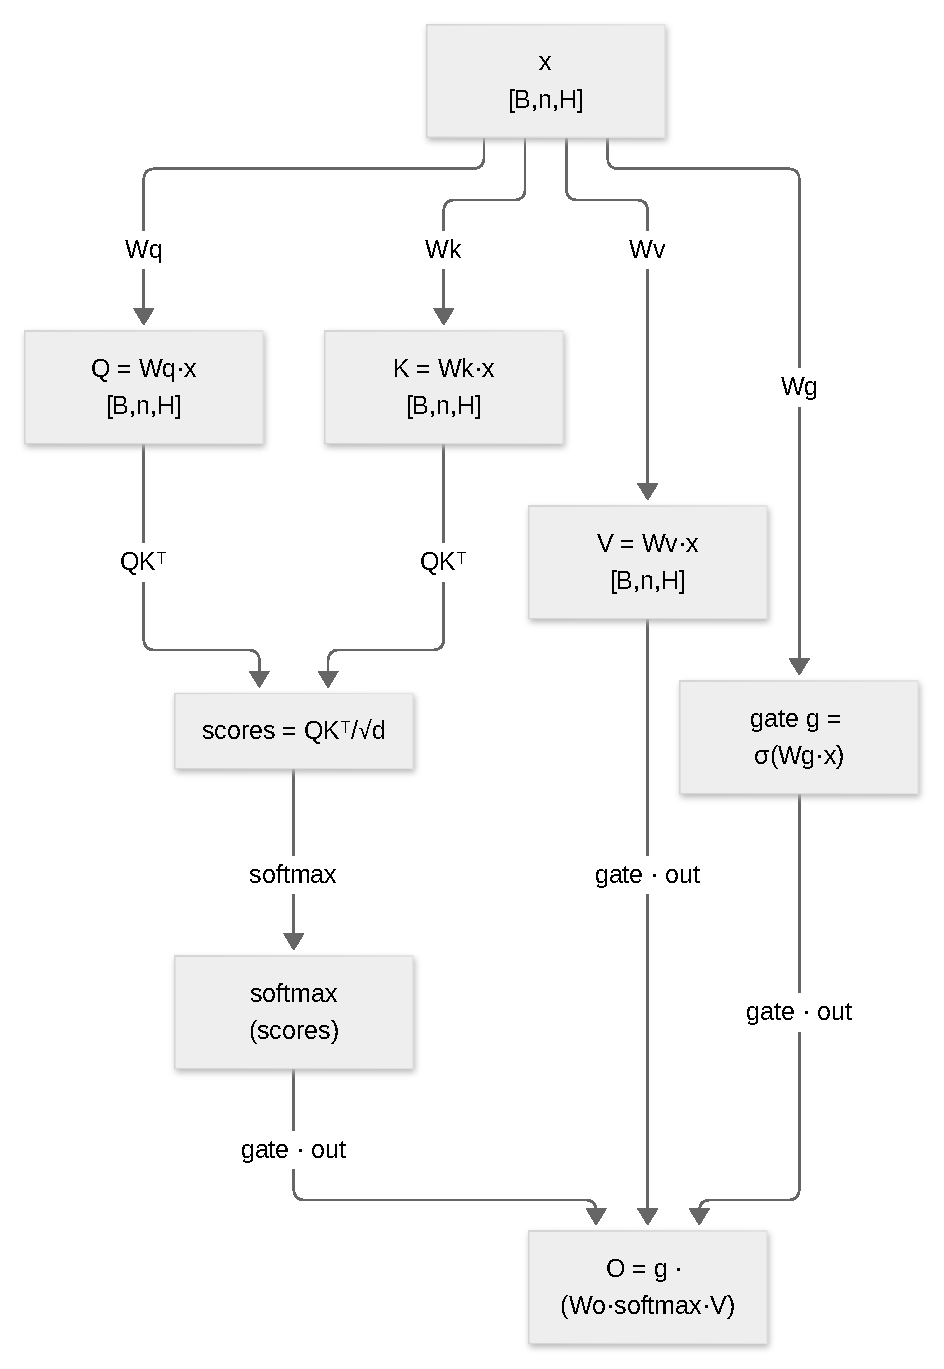
\includegraphics{figures/mixers/gated-softmax.pdf}}
\caption{Dataflow of post-SDPA gated attention: a sigmoid gate scales the softmax output before the projection.}
\label{fig:mixer-gated-softmax}
\end{figure}

\subsubsection{Mathematical Foundation}

The NeurIPS 2025 Best Paper by the Qwen team proposes applying a sigmoid gate \textbf{after} scaled dot-product attention (SDPA):
\[
\mathbf{Y} = \text{SDPA}(\mathbf{Q}, \mathbf{K}, \mathbf{V}) = \text{softmax}\left(\frac{\mathbf{Q}\mathbf{K}^\top}{\sqrt{d_k}}\right) \mathbf{V}
\]
\[
\mathbf{Y}' = \mathbf{Y} \odot \sigma\left(\mathbf{X} \mathbf{W}_\theta\right)
\]
where the gate score $\sigma(\mathbf{X} \mathbf{W}_\theta)$ can have shape $\mathbb{R}^{n \times q \times d_k}$ (element-wise gating per query head) or $\mathbb{R}^{n \times q}$ (head-wise fixed gating). Across 30+ variants and 15B MoE + 1.7B dense models trained on 3.5T tokens, the team found:

\begin{itemize}[leftmargin=*]
    \item Headwise gating adds only $\sim 1.6M$ parameters to a 15B model (negligible overhead).
    \item Effective gates are \textbf{sparse}: mean activation $\approx 0.116$ (i.e., 88\% are zero or near-zero).
    \item Gates act as query-dependent filters, suppressing low-value channels while preserving high-value signal.
    \item Gates demonstrably eliminate the \textbf{attention sink} phenomenon, where the attention pattern becomes dominated by a single early token.
\end{itemize}

\begin{algorithm}[H]
\caption{Gated Softmax Attention (Post-SDPA)}
\begin{algorithmic}[1]
\Require Queries $\mathbf{Q}$, Keys $\mathbf{K}$, Values $\mathbf{V}$; input $\mathbf{X}$
\Require Gate projection matrix $W_g \in \mathbb{R}^{d \to d_{\text{gate}}}$ where $d_{\text{gate}} \in \{1, d_k\}$
\Ensure Gated output $\mathbf{Y}'$
\State \textbf{Standard SDPA:}
\State Compute attention: $\mathbf{A} \gets \text{softmax}(\mathbf{Q}\mathbf{K}^\top / \sqrt{d_k})$ 
\State Weight values: $\mathbf{Y} \gets \mathbf{A} \mathbf{V}$
\State \textbf{Compute gates:}
\State Project input: $\mathbf{G} \gets \mathbf{X} W_g$  \Comment{shape: $[n, q, d_{\text{gate}}]$}
\State Apply sigmoid: $\mathbf{G} \gets \sigma(\mathbf{G})$ \Comment{Element-wise gating}
\State \textbf{Apply gating:}
\If{$d_{\text{gate}} = 1$}
    \State Broadcast and scale: $\mathbf{Y}' \gets \mathbf{Y} \cdot \mathbf{G}$ \Comment{Head-wise scaling}
\Else
    \Comment{$d_{\text{gate}} = d_k$}
    \State Element-wise modulation: $\mathbf{Y}' \gets \mathbf{Y} \odot \mathbf{G}$ \Comment{Per-dimension gating}
\EndIf
\Return $\mathbf{Y}'$
\end{algorithmic}
\end{algorithm}

\subsubsection{Key Findings}

\begin{itemize}[leftmargin=*]
    \item \textbf{Attention-sink suppression}: Gating breaks the feedback loop where softmax concentrates on the first token, enabling more balanced attention.
    \item \textbf{Training stability}: Models with gating tolerate larger learning rates ($+30\%$ higher stable $\eta_{max}$).
    \item \textbf{Minimal overhead}: Latency impact is only $1.6\%$ on H100 GPUs; throughput drops at most $2-3\%$.
    \item \textbf{Scaling law improvement}: Improves loss across model scales from 800M to 110B parameters consistently.
\end{itemize}

\normalsize

\subsection{7. Gated DeltaNet-2: Decoupled Channel-wise Erase and Write}

\begin{figure}[H]
\centering
\fitfigure{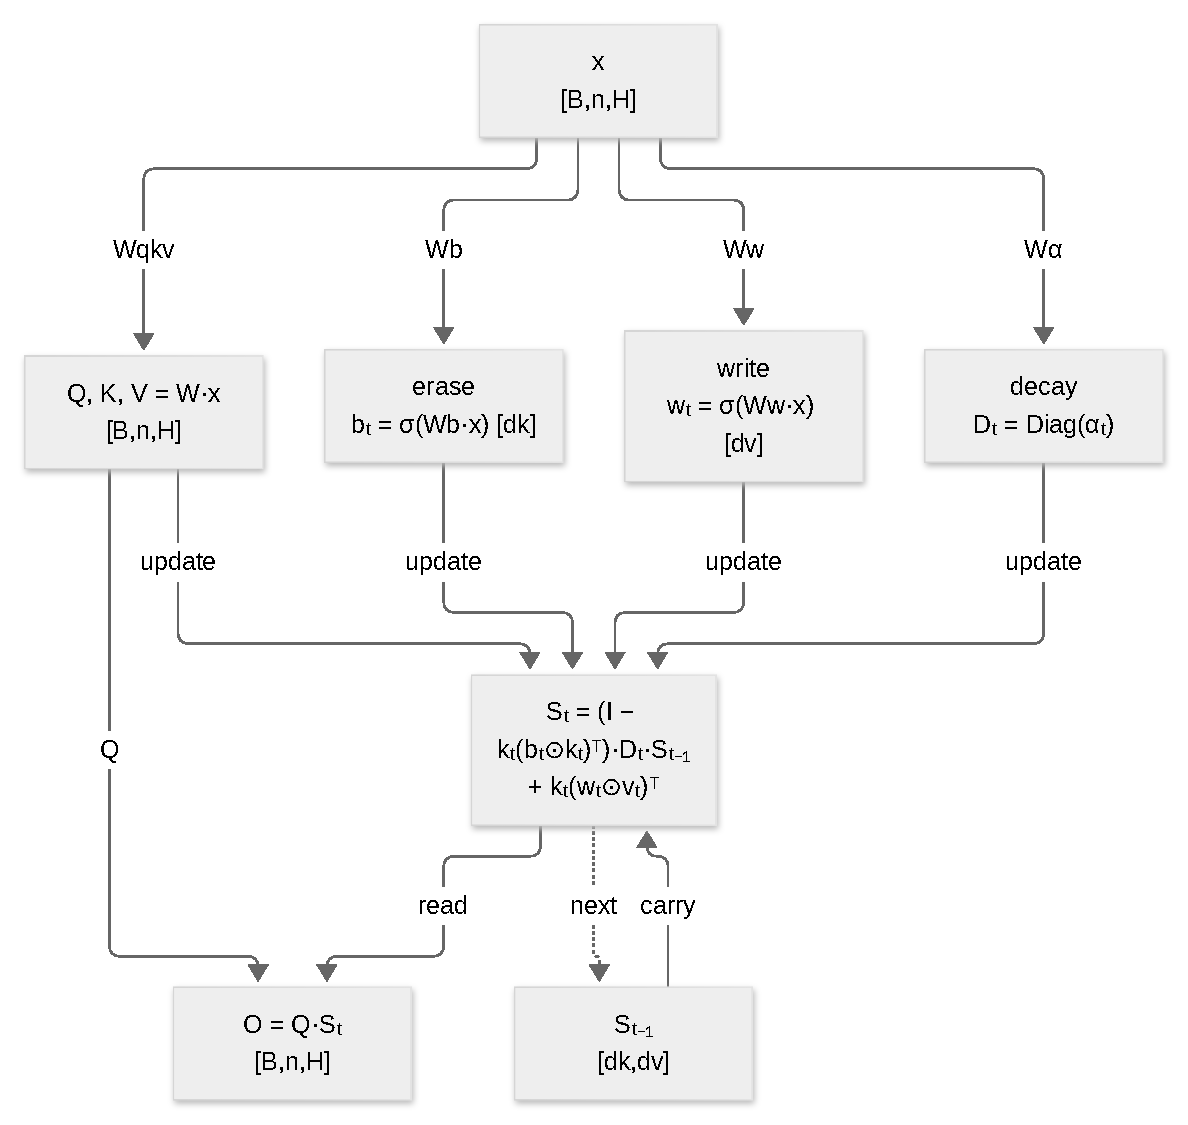
\includegraphics{figures/mixers/gated-deltanet2.pdf}}
\caption{Dataflow of Gated DeltaNet-2: decoupled channel-wise erase and write gates act inside the delta rule.}
\label{fig:mixer-gated-deltanet2}
\end{figure}

\subsubsection{Mathematical Foundation}

Gated DeltaNet-2 \citep{hatamizadeh_gated_deltanet2_2026} addresses a shared limitation of Gated DeltaNet and Kimi Delta Attention (KDA): both use a single \emph{scalar} delta gate $\beta_t$ to simultaneously control (i) how much old content is erased along the key-side read direction and (ii) how much new value is written along the value axis. Gated DeltaNet-2 \textbf{decouples} these two roles into a channel-wise erase gate $\mathbf{b}_t$ (key axis) and a channel-wise write gate $\mathbf{w}_t$ (value axis), while inheriting the channel-wise decay $\boldsymbol{\alpha}_t$ from KDA. With state $\mathbf{S}_t \in \mathbb{R}^{d_k \times d_v}$, decay $\mathbf{D}_t = \mathrm{Diag}(\boldsymbol{\alpha}_t)$, erase direction $\mathbf{e}_t = \mathbf{b}_t \odot \mathbf{k}_t$, and write target $\mathbf{z}_t = \mathbf{w}_t \odot \mathbf{v}_t$, the state update is:
\[
\mathbf{S}_t = \left(\mathbf{I} - \mathbf{k}_t \mathbf{e}_t^\top\right) \mathbf{D}_t \, \mathbf{S}_{t-1} + \mathbf{k}_t \mathbf{z}_t^\top, \qquad \mathbf{o}_t = \mathbf{S}_t^\top \mathbf{q}_t
\]
or, expanding the gate products:
\[
\mathbf{S}_t = \left(\mathbf{I} - \mathbf{k}_t (\mathbf{b}_t \odot \mathbf{k}_t)^\top\right) \mathbf{D}_t \, \mathbf{S}_{t-1} + \mathbf{k}_t (\mathbf{w}_t \odot \mathbf{v}_t)^\top
\]
The two gates are produced by independent linear projections followed by sigmoid:
\[
\mathbf{b}_t = \sigma(\mathbf{W}_b \mathbf{x}_t), \qquad \mathbf{w}_t = \sigma(\mathbf{W}_w \mathbf{x}_t)
\]
and the channel-wise decay follows a log-decay parameterization (computed in fp32 to avoid precision loss in long cumulative products):
\[
\mathbf{g}_t = \mathbf{a} - \mathrm{softplus}(\boldsymbol{\delta}), \qquad \boldsymbol{\alpha}_t = \exp(\mathbf{g}_t)
\]
The structural roles of the two gates are complementary:
\begin{itemize}[leftmargin=*]
    \item $\mathbf{b}_t$ (key axis) makes the \textbf{read direction} channel-selective: it determines which key channels are removed before writing.
    \item $\mathbf{w}_t$ (value axis) makes the \textbf{write target} channel-selective: it determines which value channels are deposited into memory.
    \item $\boldsymbol{\alpha}_t$ (per key channel) provides global decay, as in KDA.
\end{itemize}
\textbf{Reductions.} Setting $\mathbf{b}_t = \beta_t \mathbf{1}_{d_k}$ and $\mathbf{w}_t = \beta_t \mathbf{1}_{d_v}$ recovers KDA; further collapsing $\boldsymbol{\alpha}_t$ to a scalar recovers Gated DeltaNet. From the fast-weight / online-learning perspective, the update is the minimizer of:
\[
\mathcal{L}_t(\mathbf{S}) = \tfrac{1}{2}\|\mathbf{S} - \mathbf{D}_t \mathbf{S}_{t-1}\|_F^2 - 2\left\langle \mathbf{S}^\top \mathbf{k}_t,\; \mathbf{z}_t - (\mathbf{D}_t \mathbf{S}_{t-1})^\top \mathbf{e}_t \right\rangle
\]

\begin{algorithm}[H]
\caption{Gated DeltaNet-2 Recurrent Forward (Reference Form)}
\begin{algorithmic}[1]
\Require Input $\mathbf{x}_t$; prior state $\mathbf{S}_{t-1} \in \mathbb{R}^{d_k \times d_v}$
\Require Projections: $W_q, W_k, W_v, W_b, W_w$; log-decay parameters $\mathbf{a}, \boldsymbol{\delta}$
\Ensure Output $\mathbf{o}_t$ and state $\mathbf{S}_t$
\State $\mathbf{q}_t \gets \mathrm{normalize}(W_q \mathbf{x}_t)$, $\mathbf{k}_t \gets \mathrm{normalize}(W_k \mathbf{x}_t)$, $\mathbf{v}_t \gets \mathrm{silu}(W_v \mathbf{x}_t)$
\State $\mathbf{b}_t \gets \sigma(W_b \mathbf{x}_t)$ \Comment{key-axis erase gate, $\mathbb{R}^{d_k}$}
\State $\mathbf{w}_t \gets \sigma(W_w \mathbf{x}_t)$ \Comment{value-axis write gate, $\mathbb{R}^{d_v}$}
\State $\boldsymbol{\alpha}_t \gets \exp(\mathbf{a} - \mathrm{softplus}(\boldsymbol{\delta}))$ \Comment{channel-wise decay, fp32}
\State Erase direction: $\mathbf{e}_t \gets \mathbf{b}_t \odot \mathbf{k}_t$; write target: $\mathbf{z}_t \gets \mathbf{w}_t \odot \mathbf{v}_t$
\State Decay state: $\mathbf{S}_t \gets \mathrm{Diag}(\boldsymbol{\alpha}_t)\, \mathbf{S}_{t-1}$
\State Read: $\mathbf{r}_t \gets \mathbf{S}_t^\top \mathbf{e}_t$ \Comment{sum over key axis}
\State Delta-rule update: $\mathbf{S}_t \gets \mathbf{S}_t - \mathbf{k}_t \mathbf{r}_t^\top + \mathbf{k}_t \mathbf{z}_t^\top$
\State Retrieve: $\mathbf{o}_t \gets \mathbf{S}_t^\top \mathbf{q}_t$
\State Output gating: $\mathbf{o}_t \gets \mathrm{GroupNorm}(\mathbf{o}_t) \odot \mathrm{silu}(W_g \mathbf{x}_t)$
\State \Return $\mathbf{o}_t$, $\mathbf{S}_t$
\end{algorithmic}
\end{algorithm}

The chunkwise training algorithm extends KDA's WY representation by absorbing the channel-wise decay into an asymmetric delta recurrence on a decay-normalized state, enabling matmul-rich parallelism on tensor cores. Because $\mathbf{b}_t$ and $\mathbf{w}_t$ are per-channel diagonal operators varying per row, the scalar post-scaling shortcut of KDA breaks: the backward pass requires a \textbf{gate-aware WY} inversion that bakes the gates into each dot product accumulating the gradient.

\subsubsection{Empirical Performance and Trade-offs}

At 1.3B parameters trained on 100B FineWeb-Edu tokens, Gated DeltaNet-2 outperforms Mamba-2, Mamba-3, Gated DeltaNet, and KDA on language modeling, commonsense reasoning, and---most markedly---real-world and RULER long-context retrieval (especially multi-key needle-in-a-haystack). Its throughput on H100 stays near-flat ($38.0 \to 36.1$ Kt/s) as sequence length grows from 2K to 16K, where a Transformer's drops sharply. Ablations show the erase gate $\mathbf{b}_t$ accounts for most of the gain; the write gate $\mathbf{w}_t$ contributes a smaller additional improvement. The hybrid variant (recurrent Gated DeltaNet-2 + sliding-window attention) further closes the gap with pure-attention models on tasks requiring local evidence aggregation.

\begin{table}[H]
\centering
\footnotesize
\begin{tabularx}{\linewidth}{lXX}
\toprule
\textbf{Aspect} & \textbf{Strength} & \textbf{Limitation} \\
\midrule
Recall & Best-in-class among recurrent delta-rule models on multi-key NIAH. & Recurrent variant still gaps Transformer on NQ/DROP. \\
Throughput & Near-flat scaling 2K$\to$16K; small overhead vs KDA. & Requires a new gate-aware WY Triton backward kernel. \\
Memory & Constant $\mathcal{O}(d^2)$ inference state. & Neg-eigenvalue erase range $[0,2]$ gives no consistent gain at 1.3B scale. \\
\bottomrule
\end{tabularx}
\caption{Gated DeltaNet-2 trade-offs at 1.3B / 100B-token scale \citep{hatamizadeh_gated_deltanet2_2026}.}
\label{tab:gated-deltanet2-tradeoffs}
\end{table}

\normalsize

\subsection{8. Kimi Delta Attention (KDA): Channel-wise Decay Gating for the Delta Rule}

\begin{figure}[H]
\centering
\fitfigure{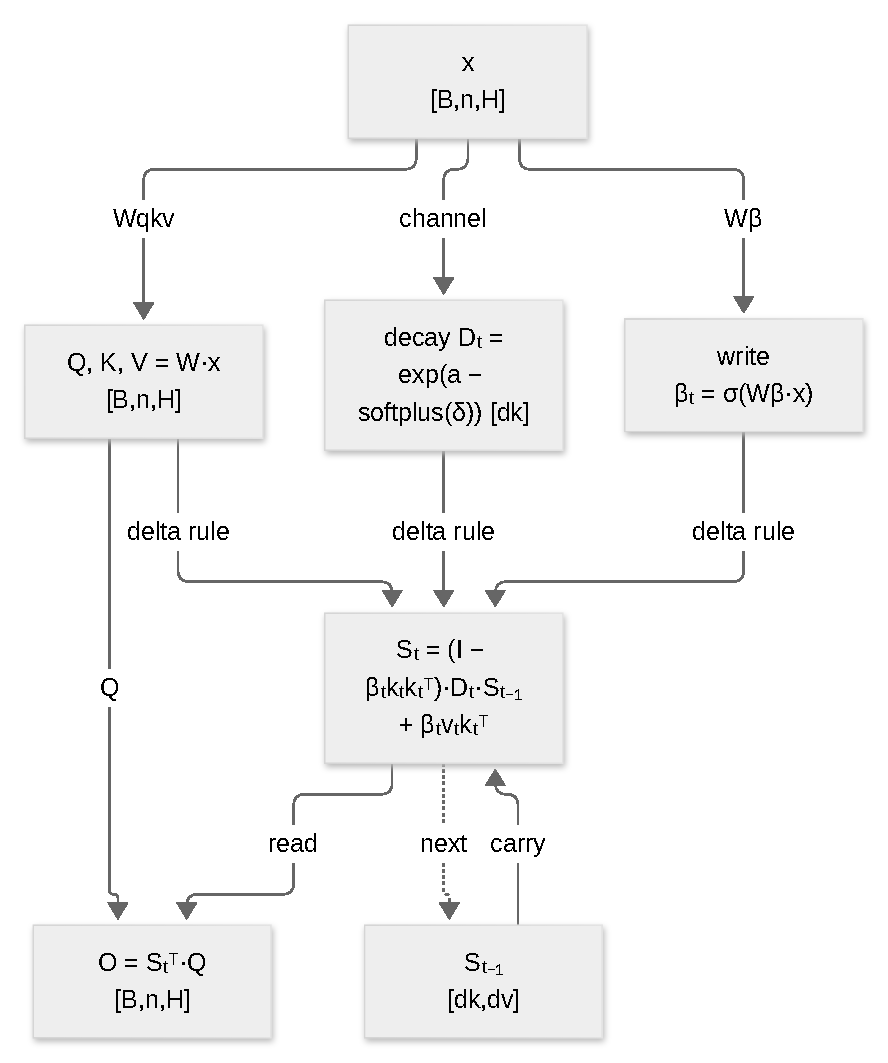
\includegraphics{figures/mixers/kda.pdf}}
\caption{Dataflow of KDA: channel-wise decay and a scalar write gate modulate the delta-rule state update.}
\label{fig:mixer-kda}
\end{figure}

\subsubsection{Mathematical Foundation}

Kimi Delta Attention \citep{kimi_kda_2025} is the core module of Kimi Linear and extends Gated DeltaNet with a finer-grained \textbf{channel-wise decay gate}. Where Gated DeltaNet uses a single scalar per-head decay $\alpha_t$ alongside the scalar delta write gate $\beta_t$, KDA replaces the scalar decay with a \textbf{per-key-channel} decay $\boldsymbol{\alpha}_t \in \mathbb{R}^{d_k}$, parameterised through a log-decay formulation and applied as a diagonal matrix $\mathbf{D}_t = \mathrm{diag}(\boldsymbol{\alpha}_t)$ before the delta-rule update. The delta rule itself retains a scalar per-head write gate $\beta_t$:
\[
\mathbf{S}_t = (\mathbf{I} - \beta_t \mathbf{k}_t \mathbf{k}_t^\top)\, \mathbf{D}_t\, \mathbf{S}_{t-1} + \beta_t \mathbf{v}_t \mathbf{k}_t^\top, \qquad \mathbf{o}_t = \mathbf{S}_t^\top \mathbf{q}_t
\]
The channel-wise decay follows a log-decay parameterisation (computed in fp32 for numerical stability over long cumulative products):
\[
\mathbf{g} = \mathbf{a} - \mathrm{softplus}(\boldsymbol{\delta}), \qquad \boldsymbol{\alpha}_t = \exp(\mathbf{g})
\]
where $\mathbf{a}$ and $\boldsymbol{\delta}$ are learned per-channel parameters. This gives each key channel an independent forgetting timescale, allowing the model to retain some channels longer than others within the same head.

\paragraph{Reduction to Gated DeltaNet}: When $\boldsymbol{\alpha}_t$ collapses to a scalar (i.e., all channels share the same decay), KDA reduces exactly to Gated DeltaNet. The channel-wise decay is thus a strict generalisation that adds per-channel selectivity on top of the scalar decay/write gating of Gated DeltaNet.

\paragraph{Chunkwise training}: A bespoke chunkwise algorithm uses a specialised \textbf{Diagonal-Plus-Low-Rank (DPLR)} variant of the transition matrix to remain hardware-efficient. The product of per-step transitions $(\mathbf{I} - \beta_t \mathbf{k}_t \mathbf{k}_t^\top)\mathbf{D}_t$ admits a DPLR decomposition that allows matmul-rich parallelism on tensor cores while preserving the channel-wise decay structure.

\begin{algorithm}[H]
\caption{Kimi Delta Attention Recurrent Forward (Reference Form)}
\begin{algorithmic}[1]
\Require Input $\mathbf{x}_t$; prior state $\mathbf{S}_{t-1} \in \mathbb{R}^{d_k \times d_v}$
\Require Projections: $W_q, W_k, W_v, W_\beta$; log-decay parameters $\mathbf{a}, \boldsymbol{\delta}$
\Ensure Output $\mathbf{o}_t$ and state $\mathbf{S}_t$
\State $\mathbf{q}_t \gets W_q \mathbf{x}_t$, $\mathbf{k}_t \gets W_k \mathbf{x}_t$, $\mathbf{v}_t \gets W_v \mathbf{x}_t$
\State $\beta_t \gets \mathrm{sigmoid}(W_\beta \mathbf{x}_t)$ \Comment{scalar per-head write gate}
\State $\boldsymbol{\alpha}_t \gets \exp(\mathbf{a} - \mathrm{softplus}(\boldsymbol{\delta}))$ \Comment{channel-wise decay, fp32}
\State $\mathbf{D}_t \gets \mathrm{diag}(\boldsymbol{\alpha}_t)$ \Comment{diagonal decay matrix}
\State Decay state: $\mathbf{S}_t \gets \mathbf{D}_t \mathbf{S}_{t-1}$
\State Read: $\mathbf{r}_t \gets \mathbf{S}_t^\top \mathbf{k}_t$ \Comment{current prediction along key}
\State Delta-rule update: $\mathbf{S}_t \gets \mathbf{S}_t - \beta_t \mathbf{k}_t \mathbf{r}_t^\top + \beta_t \mathbf{v}_t \mathbf{k}_t^\top$
\State Retrieve: $\mathbf{o}_t \gets \mathbf{S}_t^\top \mathbf{q}_t$
\State Output gating: $\mathbf{o}_t \gets \mathrm{GroupNorm}(\mathbf{o}_t) \odot \mathrm{silu}(W_g \mathbf{x}_t)$
\State \Return $\mathbf{o}_t$, $\mathbf{S}_t$
\end{algorithmic}
\end{algorithm}

\subsubsection{Empirical Performance and Trade-offs}

KDA is deployed in Kimi Linear, a hybrid model (3B activated / 48B total parameters) combining KDA layers with Multi-head Latent Attention (MLA). Kimi Linear outperforms a full-MLA baseline across all evaluated tasks, reduces the KV cache by up to $75\%$, and achieves up to $6\times$ decoding throughput for 1M-token context. The channel-wise decay is the principal driver of the gain: it allows fine-grained control over which key channels persist, improving long-context recall relative to scalar-decay Gated DeltaNet.

\begin{table}[H]
\centering
\footnotesize
\begin{tabularx}{\linewidth}{lXX}
\toprule
\textbf{Aspect} & \textbf{Strength} & \textbf{Limitation} \\
\midrule
Recall & Channel-wise decay improves long-context recall over scalar-decay baselines; deployed in Kimi Linear (3B/48B hybrid). & Recurrent matrix state $\mathcal{O}(d^2)$ is heavier than diagonal-gated linear attention. \\
Throughput & Up to $6\times$ decoding throughput at 1M context; $75\%$ KV cache reduction vs full MLA. & Requires DPLR-aware chunkwise kernels for hardware efficiency. \\
Memory & Constant $\mathcal{O}(d^2)$ inference state (matrix recurrent). & Log-decay fp32 computation adds overhead; reduction to Gated DeltaNet loses channel selectivity. \\
\bottomrule
\end{tabularx}
\caption{KDA trade-offs in Kimi Linear (3B activated / 48B total) \citep{kimi_kda_2025}.}
\label{tab:kda-tradeoffs}
\end{table}

\normalsize

\subsection{Unified Gating Principle}

All eight architectures share a common principle: \textbf{gating is a mechanism to control information flow and selective memory retention}. The specific design choices diverge along several dimensions:

\begin{enumerate}[leftmargin=*]
    \item \textbf{Location of gating}: Recurrent state updates (GLA, DeltaNet, Gated DeltaNet, Gated DeltaNet-2, HGRN2) versus softmax logit/output space (FoX, Gated Softmax, RetNet).
    \item \textbf{Granularity of control}: Dimension-wise (GLA, HGRN2 diagonal), key-specific (DeltaNet), token-wise (FoX), head-wise (Gated Softmax), or channel-wise decoupled erase/write (Gated DeltaNet-2).
    \item \textbf{Data dependence}: Fully data-dependent (GLA, DeltaNet, Gated DeltaNet, Gated DeltaNet-2, FoX, Gated Softmax) versus fixed schedules (RetNet with exponential decay).
    \item \textbf{Expressiveness trade-off}: Linear recurrent efficiency (GLA, DeltaNet, Gated DeltaNet, Gated DeltaNet-2, HGRN2, RetNet) versus full softmax expressiveness (FoX, Gated Softmax).
\end{enumerate}

\subsection{Implementation and Practical Guidance}

\subsubsection{When to Use Each Architecture}

\begin{enumerate}[leftmargin=*]
    \item \textbf{GLA}: Fast inference with moderate-to-long contexts (2K--20K tokens), when custom CUDA kernels are acceptable, and retrieval performance is not critical.
    \item \textbf{DeltaNet}: Strong associative recall and in-context learning tasks; good for synthetic tasks (MQAR) and key-value association testing.
    \item \textbf{Gated DeltaNet}: Production models requiring the best balance of recall, forgetting, and throughput (proven in Qwen3-Next; ICLR 2025).
    \item \textbf{Gated DeltaNet-2}: Long-context retrieval workloads (multi-key NIAH) where decoupled channel-wise erase/write yields the strongest recall; when a gate-aware WY kernel is available.
    \item \textbf{RetNet}: Extremely efficient inference without KV caching; suitable for edge/mobile deployments or toy models.
    \item \textbf{HGRN2}: Multi-scale temporal hierarchies; when layer-specific forget bounds are desirable.
    \item \textbf{FoX}: Length extrapolation and long-context understanding; when quadratic training is acceptable and replacing softmax is not desired.
    \item \textbf{Gated Softmax}: Quick improvement to existing softmax models with minimal code changes; best for practitioners wanting immediate gains without major refactoring.
\end{enumerate}

\subsubsection{Hardware Considerations}

\begin{table}[H]
\centering
\small
\begin{tabularx}{0.95\linewidth}{Xp{3.5cm}p{3.5cm}}
\toprule
\textbf{Hardware Target} & \textbf{Recommended Architectures} & \textbf{Notes} \\
\midrule
GPU (H100/A100) & Gated Softmax, FoX, Gated DeltaNet, Gated DeltaNet-2 & Mature softmax/linear implementations. GLA/DeltaNet require custom kernels. \\
TPU (high memory) & GLA, DeltaNet, Gated DeltaNet, Gated DeltaNet-2, HGRN2 & Hardware supports efficient matmuls; linear recurrent methods shine. \\
Mobile/Edge & RetNet, lightweight Gated Softmax & Constant-memory inference critical. \\
\bottomrule
\end{tabularx}
\end{table}


\section{Normalization, Quantization, Depth Routing, and Runtime Algorithms}
\label{sec:annex-norm-bitnet-mod}

This annex collects the implementation-level detail for normalization variants, BitNet-style ternary quantization, adaptive depth routing (Mixture-of-Depths), conditional memory (Engram), factorized embeddings, and the runtime algorithms (training-step stability controls, SBERT inference router) that support the configuration-driven pipeline. (The manifold-constrained residual connections of mHC are documented separately in Annex~9.) The main sections defer to this annex for the mathematical formulations and pseudocode; the bibliography keys cited here resolve against \texttt{docs/bibliography/}.

\subsection{Normalization Variants: LayerNorm, RMSNorm, pRMSNorm, Dynamic Tanh, Dynamic Erf, and FlashNorm}

Normalization determines how activation scale is controlled across depth. In this repository, normalization is not only a modeling choice but also a schema compatibility question, because only certain values are currently accepted by \texttt{norm\_type}. The schema contract is:
\[
\texttt{norm\_type} \in \{\texttt{layer\_norm}, \texttt{dynamic\_tanh}, \texttt{derf}, \texttt{rms\_norm}, \texttt{prms\_norm}, \texttt{flash\_norm}\}
\]
The formulations most relevant to this codebase are:

\subsubsection{LayerNorm (Baseline)}
LayerNorm \citep{ba2016layer} is the default normalizer; it centers and rescales each token by its per-token mean and variance:
\[
\mu = \frac{1}{d}\sum_{i=1}^{d} x_i, \quad \sigma^2 = \frac{1}{d}\sum_{i=1}^{d}(x_i - \mu)^2, \quad y_i = \gamma_i \frac{x_i - \mu}{\sqrt{\sigma^2 + \epsilon}} + \beta_i.
\]

\subsubsection{RMSNorm}
RMSNorm removes mean-centering and only rescales by root mean square magnitude \citep{zhang_root_2019}:
\[
\mathrm{RMS}(x)=\sqrt{\frac{1}{d}\sum_{i=1}^{d}x_i^2+\epsilon},\qquad
y_i=\gamma_i\frac{x_i}{\mathrm{RMS}(x)}.
\]
Compared with LayerNorm, RMSNorm is computationally simpler (no subtraction of feature mean) and is often used when reducing normalization overhead is important (e.g., Llama, GPT-NeoX). It has a learnable per-dimension scale $\gamma$ but no bias term.

\subsubsection{Partial RMSNorm (pRMSNorm)}
pRMSNorm \citep{zhang_root_2019} further reduces overhead by estimating the RMS from only the first $p$\% of the hidden dimensions:
\[
\mathrm{RMS}(x)=\sqrt{\frac{1}{k}\sum_{i=1}^{k}x_i^2+\epsilon},\qquad k=\lceil d\cdot p\rceil,
\]
exploiting the assumption that neurons within a layer are approximately i.i.d. The same scale $\gamma$ is then applied to all dimensions. The partial ratio $p$ is controlled by the \texttt{prms\_partial\_ratio} config field (default $6.25\%$). The paper reports that competitive results are achievable with as little as $6.25\%$ of the inputs, though gradient instability can arise with very small ratios.

\subsubsection{Dynamic Tanh (DyT)}
Dynamic Tanh proposes replacing explicit normalization with a bounded elementwise map \citep{zhu_transformers_2025}:
\[
\mathrm{DyT}(x)=\tanh(\alpha x)
\]
where $\alpha$ is learned. The core idea is that bounded nonlinear contraction can provide stable signal scaling without explicitly computing per-token normalization statistics.

\subsubsection{Dynamic Erf (Derf)}
Derf extends the same normalization-free direction by using an error-function based map \citep{chen_stronger_2025}:
\[
\mathrm{Derf}(x)=\mathrm{erf}(\alpha x+s)
\]
with learnable scale/shift. Reported results in the cited work indicate stronger performance than DyT and common normalization baselines across multiple domains.

\subsubsection{FlashNorm (Weightless RMSNorm)}
FlashNorm \citep{graef2026flashnorm} is not a new mathematical normalization; it is an \emph{exact algebraic rewrite} of the ubiquitous ``$\mathrm{RMSNorm} \to \mathrm{Linear}$'' pair that (i) eliminates the per-dimension learnable scale $\mathbf{g}$ by folding it into the subsequent linear layer's weights, and (ii) defers the scalar RMS reduction to the output of the matrix multiplication so that the matmul (matrix unit) and the RMS reduction (vector unit) execute in parallel. Three propositions formalize the rewrite.

\paragraph{Proposition 1 (Weight folding).}
Given activation $\mathbf{a}\in\mathbb{R}^{n}$, RMSNorm weight $\mathbf{g}\in\mathbb{R}^{n}$, and a subsequent linear $\mathbf{W}\in\mathbb{R}^{n\times k}$,
\[
\mathbf{z}=\mathrm{RMSNorm}(\mathbf{a})\mathbf{W}=\frac{\mathbf{a}}{\mathrm{RMS}(\mathbf{a})}\mathbf{W}^{*},\qquad
W^{*}_{i,j}=g_{i}\cdot W_{i,j}\ \Leftrightarrow\ \mathbf{W}^{*}=\operatorname{diag}(\mathbf{g})\mathbf{W}.
\]
The per-dimension scale $\mathbf{g}$ becomes redundant and is folded into $\mathbf{W}$ once at load time. The standalone \texttt{FlashNorm} module in this repository applies this directly: it has \emph{no learnable parameters} (the scale is meant to be absorbed by the downstream projection).

\paragraph{Proposition 2 (Deferred normalization).}
For a bias-free linear $\mathbf{W}^{*}$, scalar--matrix commutativity yields
\[
\frac{\mathbf{a}}{\mathrm{RMS}(\mathbf{a})}\mathbf{W}^{*}=\left(\mathbf{a}\mathbf{W}^{*}\right)\cdot\frac{1}{\mathrm{RMS}(\mathbf{a})}.
\]
The matmul $\mathbf{a}\mathbf{W}^{*}$ and the RMS reduction are independent of each other; on hardware with distinct matrix and vector execution units they execute in parallel, and only a single vector--scalar multiply synchronizes them. The fused module \texttt{FlashNormLinear} implements this rewrite: on the bias-free path it computes the matmul on the \emph{un-normalized} input and multiplies the result by the per-token reciprocal RMS. When the linear has a bias $\mathbf{c}$, the rewrite is no longer exact (Remark 1 of the paper): $\left(\mathbf{a}\mathbf{W}^{*}+\mathbf{c}\right)/\mathrm{RMS}(\mathbf{a})\neq\mathbf{a}\mathbf{W}^{*}/\mathrm{RMS}(\mathbf{a})+\mathbf{c}$; the layer then applies the scalar to the input first and lets the linear add its bias as usual.

\paragraph{Proposition 3 (RMS cancellation).}
By RMS scale invariance, $\mathrm{RMS}(\alpha\mathbf{a})=\alpha\,\mathrm{RMS}(\mathbf{a})$. Therefore an ``$\mathrm{RMSNorm}\to\mathrm{Linear}\to\mathrm{RMSNorm}$'' pattern allows the \emph{first} RMSNorm to be dropped entirely:
\[
\mathrm{RMSNorm}\!\left(\frac{\mathbf{a}}{\mathrm{RMS}(\mathbf{a})}\mathbf{W}^{*}\right)=\mathrm{RMSNorm}\!\left(\mathbf{a}\mathbf{W}^{*}\right).
\]
This cancellation is relevant for QKV-normalization (Gemma~4) and MLA latent normalization (DeepSeek-V2, Mistral Small~4); it is not auto-applied in this repository but is documented for completeness.

\paragraph{Partial-RMS composition.}
FlashNorm composes naturally with the pRMSNorm trick (§\ref{sec:annex-norm-bitnet-mod}, pRMSNorm subsection): when \texttt{flashnorm\_partial\_ratio} $=p>0$, the RMS is estimated from the first $k=\lceil d\cdot p\rceil$ dimensions of the input only, reducing the cost of the vector-unit RMS reduction further.

\paragraph{BitNet interaction.}
Folding a floating-point $\mathbf{g}$ into BitNet's ternary weight tensor $\{-1,0,+1\}$ \citep{wang_bitnet_2023} would destroy the quantization, and BitLinear applies its own internal LayerNorm before activation quantization which needs the normalized input. The fused module \texttt{FlashNormBitLinear} therefore falls back to the sequential composition $\mathrm{FlashNorm}\to\mathrm{BitLinear}$: the matmul and the RMS reduction still execute in parallel, but the post-matmul scalar multiply of Prop.~2 is sacrificed. Folding f.p.~$\mathbf{g}$ into a 1.58-bit weight tensor is left to future kernel-level work.

\paragraph{PyTorch pseudocode.}
\begin{algorithmic}[1]
\State \textbf{Input:} activation $\mathbf{a}\in\mathbb{R}^{T\times n}$, RMSNorm weight $\mathbf{g}\in\mathbb{R}^{n}$, linear $\mathbf{W}\in\mathbb{R}^{n\times k}$, bias $\mathbf{c}\in\mathbb{R}^{k}$ or \texttt{None}
\State \texttt{// Prop. 1: weight folding at load time}
\State $\mathbf{W}^{*}\gets \mathbf{g}\odot\mathbf{W}$ \Comment{column-wise; \texttt{g.unsqueeze(0) * W} in PyTorch}
\State $\mathbf{g}\gets \mathbf{1}$ \Comment{the standalone norm is now weightless}
\State \texttt{// Prop. 2: forward pass with deferred RMS (bias-free path)}
\State $\mathbf{b}\gets \mathbf{a}\mathbf{W}^{*\top}$ \Comment{matrix unit / tensor cores}
\State $\mathrm{rms\_inv}\gets \mathrm{rsqrt}(\mathrm{mean}(\mathbf{a}^{2})+\varepsilon)$ \Comment{vector unit, independent of $\mathbf{b}$}
\If{$\mathbf{c}=\texttt{None}$}
    \State \textbf{return} $\mathbf{b}\cdot\mathrm{rms\_inv}$ \Comment{single vector--scalar multiply}
\Else
    \State \texttt{// Remark 1: bias path is sequential; matmul and RMS still parallelize}
    \State \textbf{return} $(\mathbf{a}\cdot\mathrm{rms\_inv})\mathbf{W}^{*\top}+\mathbf{c}$
\EndIf
\end{algorithmic}

\paragraph{Reported latency (NVIDIA T4 GPU).}
The paper reports the following speedups on the norm-then-project operation, with an adaptive dispatch that falls back to the sequential path in the memory-bound (decode) regime:

\scriptsize
\begin{tabular}{llrrrr}
\toprule
\textbf{Scale} & \textbf{Tokens} & \textbf{Sequential (ms)} & \textbf{FlashNorm (ms)} & \textbf{Speedup} & \textbf{Notes} \\
\midrule
SmolLM2-135M & 4096 & 0.704 & 0.468 & $+33.6\%$ & compute-bound (prefill) \\
SmolLM2-135M & 8192 & 0.929 & 0.599 & $+35.5\%$ & compute-bound (prefill) \\
Llama-7B     & 1024 & 1.882 & 1.654 & $+12.1\%$ & compute-bound (prefill) \\
Llama-7B     & 4096 & 7.628 & 6.570 & $+13.9\%$ & compute-bound (prefill) \\
\bottomrule
\end{tabular}
\normalsize

\paragraph{Zero-loss weight folding validation.}
Weight folding (Prop.~1) is mathematically exact; the paper verified bit-identical outputs on three open-weight checkpoints:

\scriptsize
\begin{tabular}{lll}
\toprule
\textbf{Model} & \textbf{Precision} & \textbf{Result} \\
\midrule
SmolLM2-135M & fp16 & max diff $=0.0$, cosine sim $=1.0$, identical text \\
Llama-3.2-1B & fp32 & bit-identical greedy generation \\
Llama-3.1-8B & fp32 & bit-identical greedy generation \\
\bottomrule
\end{tabular}
\normalsize
Quality preservation on \texttt{lm-evaluation-harness} (wikitext word\_ppl, MMLU 5-shot, HellaSwag 0-shot) stays within benchmark noise (worst $\Delta=+0.0017$ word\_ppl).

\subsubsection{Comparison}
\scriptsize
\begin{longtable}{p{2.2cm}p{3.4cm}p{2.0cm}p{4.0cm}}
\toprule
\textbf{Method} & \textbf{Formula} & \textbf{Stats Needed} & \textbf{Notes} \\
\midrule
\endhead
LayerNorm & $\gamma_i (x_i - \mu)/\sqrt{\sigma^2 + \epsilon} + \beta_i$ & mean + variance & Default; full centering and rescaling \citep{ba2016layer}. \\
RMSNorm & $\gamma_i x_i/\sqrt{\frac{1}{d}\sum_j x_j^2+\epsilon}$ & RMS only & Lower overhead; widely used baseline \citep{zhang_root_2019}. \\
pRMSNorm & $\gamma_i x_i/\sqrt{\frac{1}{k}\sum_{j\le k} x_j^2+\epsilon}$ & Partial RMS & RMS from first $p$\% of dims; \texttt{prms\_partial\_ratio} default $6.25\%$ \citep{zhang_root_2019}. \\
Dynamic Tanh & $\tanh(\alpha x)$ & none & Normalization-free bounded transform; drop-in replacement \citep{zhu_transformers_2025}. \\
Dynamic Erf & $\mathrm{erf}(\alpha x+s)$ & none & Normalization-free alternative; improves over DyT \citep{chen_stronger_2025}. \\
FlashNorm & $x_i/\sqrt{\frac{1}{d}\sum_j x_j^2+\epsilon}$ (weightless) & RMS only & Exact rewrite of RMSNorm$\to$Linear: folds $\mathbf{g}$ into $\mathbf{W}$ (Prop.~1), defers scalar RMS to matmul output (Prop.~2); 12--35\% latency reduction on T4 GPU \citep{graef2026flashnorm}. \\
\bottomrule
\end{longtable}
\normalsize

\subsection{BitNet Ternary Quantization Path}

When \texttt{use\_bitnet=true}, BitLinear layers replace standard \texttt{nn.Linear} with ternary weight quantization ($-1, 0, +1$) following BitNet \citep{wang_bitnet_2023}. Given weight tensor $W$, a practical scaling is:
\[
s=\text{mean}(|W|),\qquad
\tilde{W}=\text{clip}\left(\text{round}\left(\frac{W}{s}\right),-1,1\right).
\]
The packed mapping uses two bits per weight symbol for storage efficiency. This enables significant compression ($\sim 32\times$ versus FP32) but is experimental and may affect model quality; it is best suited for inference deployment.

Activation quantization for the INT8 path is:
\[
q=\text{round}\left(x\cdot\frac{127}{\max(|x|)+\epsilon}\right),\qquad q\in[-128,127]
\]
with dequantization $x\approx q/\alpha$. For $N$ parameters, size estimates before metadata and packing overhead are:
\[
\text{FP32 size}\approx 4N,\quad \text{FP16 size}\approx 2N,\quad \text{1.58-bit size}\approx \frac{1.58}{8}N
\]
which aligns with lightweight deployment goals \citep{samson_lightweight_2026,bravin_embbert_2026}.

\subsection{Mixture-of-Depths (MoD) Token Routing}

When \texttt{use\_mixture\_of\_depths=true}, each transformer block scores tokens with a lightweight router. Only the top \texttt{mixture\_of\_depths\_capacity\_ratio} subset is updated; skipped tokens pass through unchanged \citep{zhu2026mixtureofdepthsattention}. This allocates more depth to salient tokens, reducing per-layer compute.

\begin{algorithmic}[1]
\State \textbf{Input:} hidden states $H \in \mathbb{R}^{n \times d}$, router $R$, capacity ratio $\rho$
\State $\text{scores} \gets R(H)$ \Comment{per-token router score}
\State $\mathcal{S} \gets \texttt{top-k}(\text{scores}, k=\lceil \rho \cdot n \rceil)$ \Comment{select salient subset}
\State $H_{\text{update}} \gets \texttt{block}(H[\mathcal{S}])$ \Comment{apply transformer block to selected tokens}
\State $H[\mathcal{S}] \gets H_{\text{update}}$ \Comment{write back; non-selected tokens bypass the block}
\State \textbf{Output:} $H$ \Comment{auxiliary load-balancing loss added from \texttt{mixture\_of\_depths\_router\_aux\_loss\_weight}}
\end{algorithmic}

\subsubsection{Configuration}
\begin{itemize}[leftmargin=*]
    \item \texttt{use\_mixture\_of\_depths}: bool --- enable MoD token routing.
    \item \texttt{mixture\_of\_depths\_capacity\_ratio}: float in $(0, 1]$ --- fraction of tokens updated per layer.
    \item \texttt{mixture\_of\_depths\_router\_aux\_loss\_weight}: float $\ge 0$ --- auxiliary loss weight for router regularization.
\end{itemize}

\subsection{Engram Conditional Memory}

\begin{figure}[H]
\centering
\fitfigure{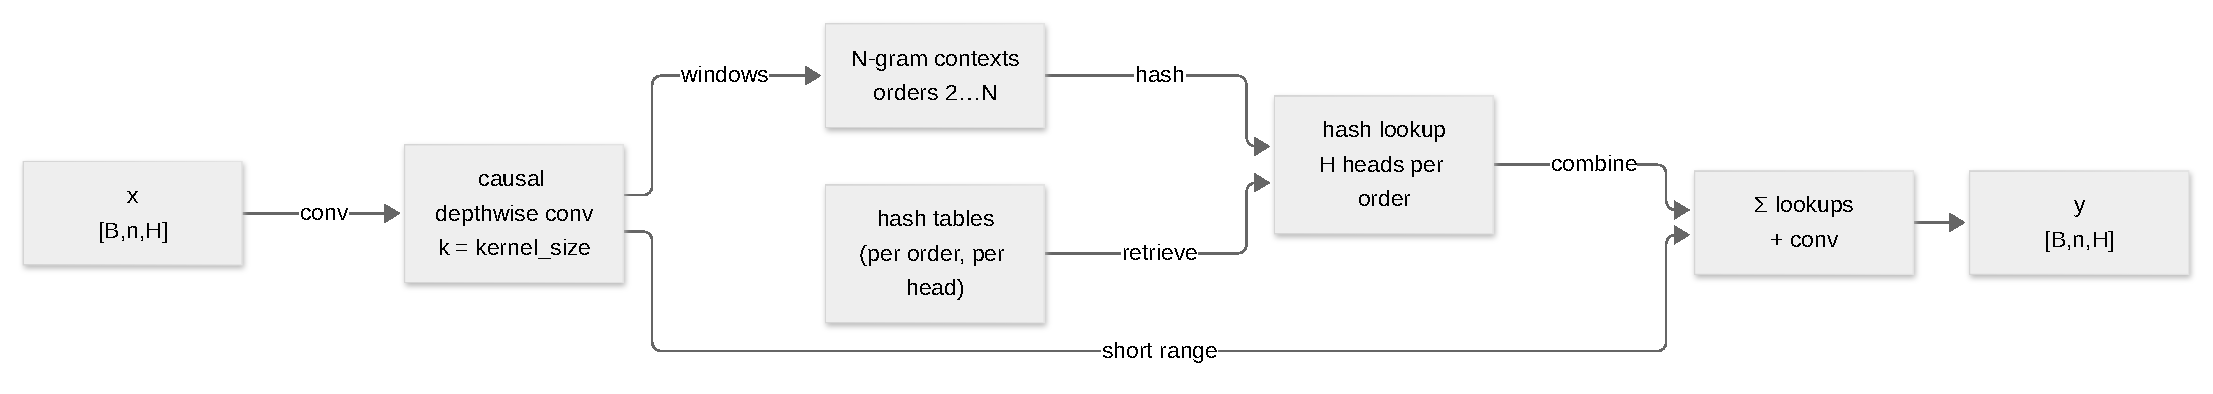
\includegraphics{figures/mixers/engram.pdf}}
\caption{Dataflow of Engram conditional memory: a causal depthwise convolution supplies short-range context, N-gram hash lookups retrieve per-order embeddings, and the lookups are summed with the convolution output.}
\label{fig:mixer-engram}
\end{figure}

Engram (\texttt{engram\_attn}) implements conditional memory via scalable N-gram lookup \citep{cheng2026conditionalmemoryscalablelookup}. It builds hash-based lookup tables for N-gram contexts from size 2 up to \texttt{engram\_max\_ngram\_size}, with independent hash heads per N-gram order. A causal depthwise convolution (\texttt{engram\_kernel\_size}) provides short-range context before the N-gram lookup.

\begin{algorithmic}[1]
\State \textbf{Input:} token stream $x_{1:n}$, N-gram orders $\{2, \ldots, N\}$, hash heads per order $H$
\State $h_{\text{conv}} \gets \text{DepthwiseConv1d}(x_{1:n}, k=\texttt{engram\_kernel\_size})$ \Comment{short-range context}
\For{each N-gram order $k \in \{2, \ldots, N\}$}
    \State $\text{ctx}_t^{(k)} \gets x_{t-k+1:t}$ \Comment{N-gram context window}
    \State $\text{lookup}^{(k)}_t \gets \text{HashTable}^{(k)}[\text{hash}(\text{ctx}_t^{(k)})]$ \Comment{per-head retrieval, $H$ heads per order}
\EndFor
\State $y_t \gets \sum_{k} \text{lookup}^{(k)}_t + h_{\text{conv},t}$ \Comment{combine conditional memories}
\State \textbf{Output:} $y_{1:n}$
\end{algorithmic}

\subsubsection{Configuration}
\begin{itemize}[leftmargin=*]
    \item \texttt{engram\_max\_ngram\_size}: int $\ge 2$ --- highest N-gram order (default 3).
    \item \texttt{engram\_n\_heads\_per\_ngram}: int $\ge 1$ --- hash heads per N-gram order (default 4).
    \item \texttt{engram\_embed\_dim\_per\_head}: int $\ge 1$ --- embedding dim per hash head (default 32).
    \item \texttt{engram\_kernel\_size}: int $\ge 1$ --- causal depthwise conv kernel width (default 4).
    \item \texttt{engram\_seed}: int --- hash seed for reproducibility (default 42).
\end{itemize}
Total Engram hidden size = $(\texttt{max\_ngram\_size} - 1) \times \texttt{n\_heads\_per\_ngram} \times \texttt{embed\_dim\_per\_head}$.

\subsection{Factorized Embeddings and Embedding Convolution}

\subsubsection{Factorized Embeddings}
When \texttt{use\_factorized\_embedding=true}, the embedding matrix is factorized into two smaller matrices, reducing parameters from $O(V \times H)$ to $O(V \times R + R \times H)$ where $R = \texttt{factorized\_embedding\_dim}$.
\begin{itemize}[leftmargin=*]
    \item \texttt{use\_factorized\_embedding}: bool --- enable factorization.
    \item \texttt{factorized\_embedding\_dim}: int $\ge 1$ --- intermediate dimension (typical: 64--256).
\end{itemize}

\subsubsection{Embedding Convolution}
When \texttt{use\_embedding\_conv=true}, a depthwise Conv1d is applied over the embedding stream before the first transformer block, with kernel size \texttt{embedding\_conv\_kernel}. This provides a lightweight local-context filter on token embeddings.

\subsection{Training-Step Stability Controls}

The schema-driven training step applies gradient accumulation, global-norm clipping, post-clip explosion guards, and bounded NaN/Inf retries. The accumulated gradient is:
\[
g_{\text{acc}}=\frac{1}{K}\sum_{i=1}^{K} g_i,\quad K=\texttt{gradient\_accumulation\_steps}
\]
\[
g_{\text{clip}} = g_{\text{acc}}\cdot
\min\left(1,\frac{\tau}{\|g_{\text{acc}}\|_2+\epsilon}\right),\quad
\tau=\texttt{grad\_clip\_max\_norm}
\]
then overflow guards use \texttt{inf\_post\_clip\_threshold} and retry logic bounded by \texttt{max\_nan\_retries}.

\begin{algorithm}[t]
\caption{Schema-Driven Training Step with Stability Controls}
\begin{algorithmic}[1]
\Require Batch stream, config $C$
\State Initialize retry counter $r\gets 0$
\For{each optimizer step}
    \State Accumulate gradients for $K=C.\texttt{gradient\_accumulation\_steps}$ micro-batches
    \State Apply global norm clipping with $\tau=C.\texttt{grad\_clip\_max\_norm}$
    \If{post-clip gradient exceeds $C.\texttt{inf\_post\_clip\_threshold}$ or NaN/Inf detected}
        \If{$r < C.\texttt{max\_nan\_retries}$}
            \State restore safe state / skip step; $r \gets r+1$
            \State \textbf{continue}
        \Else
            \State stop training with failure state
        \EndIf
    \EndIf
    \State run optimizer step selected by \texttt{optimizer\_class}
    \State update scheduler (\texttt{cosine}, \texttt{constant}, or \texttt{linear\_warmup\_then\_constant})
    \If{step mod \texttt{checkpoint\_every\_n\_steps}$=0$}
        \State save rolling checkpoint and prune to \texttt{max\_rolling\_checkpoints}
    \EndIf
    \State update best checkpoints up to \texttt{num\_best\_checkpoints}
    \State emit CSV + telemetry following \texttt{gradient\_log\_interval} and \texttt{telemetry\_log\_interval}
\EndFor
\end{algorithmic}
\end{algorithm}

\subsection{SBERT Inference Mode Router}

The SBERT inference dispatcher selects among similarity scoring, corpus search, clustering, and persistent encoding modes over a single shared encoder \citep{reimers_sentence-bert_2019}. The cosine similarity and regression loss are:
\[
\text{cos}(e_1,e_2)=\frac{e_1^\top e_2}{\|e_1\|\|e_2\|},\qquad
\mathcal{L}_{\text{cos}}=\left(\text{cos}(e_1,e_2)-y\right)^2
\]
with $y\in[-1,1]$ in this pipeline.

\begin{algorithm}[t]
\caption{SBERT Inference Mode Router}
\begin{algorithmic}[1]
\Require mode $m$, model $E$, inputs $X$
\If{$m=\texttt{similarity}$}
    \State return $\cos(E(x_1),E(x_2))$
\ElsIf{$m=\texttt{search}$}
    \State return top-$k$ by dot-product/cosine against corpus embeddings
\ElsIf{$m=\texttt{cluster}$}
    \State return clustering labels over $E(X)$
\Else
    \State return serialized embeddings $E(X)$
\EndIf
\end{algorithmic}
\end{algorithm}
\section{Activation Functions}
\label{sec:annex-activation-functions}

This annex documents the complete activation-function library available in the
model. The library provides \textbf{43 feed-forward activation functions}: 40
elementwise activations and 3 gated-FFN variants. Activations are grouped into
five families, following the taxonomy of Dubey et al.~\citep{dubey2021activations}
and the analytic overview of Lederer~\citep{lederer2021activations}, augmented
with the learnable Rational Activation Function (RAF) of
Fang et al.~\citep{fang2023raft}.

The selection is driven by the \texttt{ffn\_activation} configuration field (a
string enum) and dispatched at runtime by a factory function that mirrors the
normalization-layer dispatch (Annex~7).

\[
\texttt{ffn\_activation} \in \{\texttt{silu},\;\texttt{gelu},\;\dots,\;
\texttt{raf},\;\texttt{swiglu},\;\texttt{geglu},\;\texttt{reglu}\}
\]

\subsection{Classical / Sigmoid--Tanh Family (12 activations)}

The classical family comprises smooth, stateless activations rooted in
logistic and algebraic functions~\citep{lederer2021activations,dubey2021activations}.
All share monotonicity or near-monotonicity and are continuously differentiable.

{\footnotesize
\begin{align}
  \text{Sigmoid}(x) &= \frac{1}{1+e^{-x}}
    & \text{Range: } (0,1),\;\text{monotonic, smooth}
    & \quad \text{\citep{lederer2021activations}} \\[4pt]
  \text{Tanh}(x) &= \frac{e^{x}-e^{-x}}{e^{x}+e^{-x}} = 2\,\sigma(2x)-1
    & \text{Range: } (-1,1),\;\text{monotonic, smooth}
    & \quad \text{\citep{lederer2021activations}} \\[4pt]
  \text{Arctan}(x) &= \arctan(x)
    & \text{Range: } (-\tfrac{\pi}{2},\tfrac{\pi}{2}),\;\text{monotonic, smooth}
    & \quad \text{\citep{lederer2021activations}} \\[4pt]
  \text{Softsign}(x) &= \frac{x}{1+|x|}
    & \text{Range: } (-1,1),\;\text{smooth, once-diff.\ at 0}
    & \quad \text{\citep{lederer2021activations}} \\[4pt]
  \text{Elliott}(x) &= \frac{x}{1+|x|}
    & \text{Alias of Softsign (survey ``elliottsig'' notation)}
    & \quad \text{\citep{lederer2021activations}} \\[4pt]
  \text{Identity}(x) &= x
    & \text{Range: } (-\infty,\infty),\;\text{linear, }C^\infty
    & \quad \text{(internal)}
\end{align}
}  % end size group

{\scriptsize
\begin{align}
  \text{Softplus}(x) &= \log(1+e^{x})
    & \text{Range: } [0,\infty),\;\text{smooth, }C^\infty
    & \quad \text{\citep{glorot2011softplus}} \\[4pt]
  \text{Mish}(x) &= x\,\tanh\!\big(\text{softplus}(x)\big)
    = x\,\tanh\!\big(\log(1+e^{x})\big)
    & \text{Range: } [\approx{-0.31},\infty),\;\text{non-monotonic, smooth}
    & \quad \text{\citep{misra2019mish}} \\[4pt]
  \text{GELU}(x) &= x\,\Phi(x) = x\cdot\tfrac{1}{2}\Big(1+\text{erf}\!\Big(\frac{x}{\sqrt{2}}\Big)\Big)
    & \text{Range: } (\approx{-0.17},\infty),\;\text{smooth, probabilistic}
    & \quad \text{\citep{hendrycks2016gelu}} \\[4pt]
  \text{GELU-tanh}(x) &= \tfrac{x}{2}\Big(1+\tanh\!\Big(\sqrt{\tfrac{2}{\pi}}
    (x+0.044715\,x^{3})\Big)\Big)
    & \text{Tanh approximation of GELU (faster)}
    & \quad \text{\citep{hendrycks2016gelu}} \\[4pt]
  \text{ReLU}(x) &= \max(0,x)
    & \text{Range: } [0,\infty),\;\text{piecewise-linear, non-smooth at 0}
    & \quad \text{\citep{nair2010relu}} \\[4pt]
  \text{SiLU}(x) &= x\,\sigma(x) = \frac{x}{1+e^{-x}}
    & \text{Range: } (\approx{-0.278},\infty),\;\text{non-monotonic, smooth}
    & \quad \text{\citep{elfwing2018silu}}
\end{align}
}  % end size group

\noindent\textbf{SiLU} (Sigmoid Linear Unit) is the default activation
(\texttt{ffn\_activation=silu}). When $\beta=1$, the parametric Swish reduces
to SiLU. GELU and its tanh approximation are the standard in BERT and
GPT-2/3~\citep{hendrycks2016gelu}. Mish~\citep{misra2019mish} is a
self-regularized, non-monotonic composition of Softplus and Tanh, reported to
outperform Swish on several benchmarks.

\subsection{Rectified Family (12 activations)}

The rectifier family extends ReLU with learnable slopes, bounded variants, and
rectified-hyperbolic forms~\citep{nair2010relu,dubey2021activations}.

{\scriptsize
\begin{align}
  \text{LeakyReLU}(x) &= \begin{cases} x & x\ge 0 \\ a\,x & x < 0 \end{cases},
    \quad a=0.01
    & \text{Range: } (-\infty,\infty)
    & \quad \text{\citep{maas2013leakyrelu}} \\[4pt]
  \text{ReLU6}(x) &= \min\!\big(\max(0,x),\,6\big)
    & \text{Range: } [0,6],\;\text{bounded, fixed-point friendly}
    & \quad \text{\citep{howard2017mobile}} \\[4pt]
  \text{HardSwish}(x) &= x\cdot\frac{\text{ReLU6}(x+3)}{6}
    & \text{Range: } (\approx{-1.67},\infty),\;\text{cheap Swish approx.}
    & \quad \text{\citep{howard2019hardswish}} \\[4pt]
  \text{PReLU}(x) &= \max(0,x)+\mathbf{p}\odot\min(0,x)
    & \text{Learnable per-channel slope } \mathbf{p},\;\text{init 0.25}
    & \quad \text{\citep{he2015prelu}} \\[4pt]
  \text{AbsReLU}(x) &= \max(0,x)-\max(0,-x) = x\;\text{(sign-ramp)}
    & \text{Range: } (-\infty,\infty)
    & \quad \text{\citep{dubey2021activations}} \\[4pt]
  \text{NLReLU}(x) &= \beta\,\log\!\big(1+\max(0,x)\big)
    & \text{Range: } [0,\infty),\;\beta=1.0,\;\text{logarithmic compression}
    & \quad \text{\citep{dubey2021activations}}
\end{align}
}  % end size group

{\scriptsize
\begin{align}
  \text{BReLU}(x) &= \min\!\big(\max(0,x),\,t\big),\quad t=1.0
    & \text{Range: } [0,t],\;\text{bounded rectifier}
    & \quad \text{\citep{dubey2021activations}} \\[4pt]
  \text{VReLU}(x) &= |x|
    & \text{Range: } [0,\infty),\;\text{symmetric rectifier}
    & \quad \text{\citep{dubey2021activations}} \\[4pt]
  \text{Hexpo}(x) &= a\,\max(0,x)-c\,\max(0,-x),\quad a{=}c{=}1.0
    & \text{Asymmetric two-sided rectifier}
    & \quad \text{\citep{dubey2021activations}} \\[4pt]
  \text{PenalizedTanh}(x) &= \max\!\big(0,\,\tanh(x)\big)
    & \text{Range: } [0,1),\;\text{rectified tanh, smooth near 0}
    & \quad \text{\citep{dubey2021activations}} \\[4pt]
  \text{DisReLU}(x) &= \max(0,\,x-\delta),\quad \delta=0.0
    & \text{Right-shifted ReLU hinge}
    & \quad \text{\citep{dubey2021activations}} \\[4pt]
  \text{LiSHT}(x) &= x\,\tanh(x)
    & \text{Range: } [0,\infty)\;\text{(magnitude), non-monotonic, smooth}
    & \quad \text{\citep{roy2019lisht}}
\end{align}
}  % end size group

\noindent\textbf{PReLU}~\citep{he2015prelu} makes the negative slope a
per-channel learnable parameter, enabling the network to learn the optimal
leak per feature. \textbf{HardSwish}~\citep{howard2019hardswish} is the cheap
Swish approximation used in MobileNetV3. \textbf{ReLU6}~\citep{howard2017mobile}
was introduced in MobileNetV1 for fixed-point quantization friendliness.

\subsection{Exponential / ELU Family (12 activations)}

The exponential-linear family provides smooth negative saturation and
self-normalizing variants~\citep{clevert2016elu,klambauer2017selu,dubey2021activations}.
Several members introduce per-channel learnable parameters.

\begin{align}
  \text{ELU}(x) &= \begin{cases} x & x\ge 0 \\ \alpha(e^{x}-1) & x<0 \end{cases},
    \quad \alpha=1.0
    & \text{Range: } (-\alpha,\infty)
    & \quad \text{\citep{clevert2016elu}} \\[4pt]
  \text{SELU}(x) &= \lambda\,\text{ELU}_{\alpha'}(x)
    & \alpha'{\approx}1.6733,\;\lambda{\approx}1.0507,
    & \quad \text{\citep{klambauer2017selu}} \\
  & & \text{self-normalizing (mean 0, var 1)} & \notag \\[4pt]
  \text{CELU}(x) &= \begin{cases} x & x\ge 0 \\ \alpha(e^{x/\alpha}-1) & x<0 \end{cases},
    \quad \alpha=1.0
    & \text{Once-diff.\ at 0 for any } \alpha
    & \quad \text{\citep{barron2017celu}} \\[4pt]
  \text{PELU}(x) &= \begin{cases} \tfrac{\alpha}{\beta}\,x & x\ge 0 \\
    \alpha(e^{x/\beta}-1) & x<0 \end{cases}
    & \alpha,\beta\text{ learnable per-channel}
    & \quad \text{\citep{trottier2017pelu}} \\[4pt]
  \text{MPELU}(x) &= \text{ReLU}(x)+\beta\cdot\text{ELU}_{\alpha}(x)\cdot\mathbb{1}_{x<0}
    & \alpha,\beta\text{ learnable per-channel}
    & \quad \text{\citep{dubey2021activations}}
\end{align}

{\footnotesize
\begin{align}
  \text{FELU}(x) &= \begin{cases} x & x\ge 0 \\ \alpha(e^{x}-1) & x<0 \end{cases}
    & \alpha\text{ learnable, clamped to } [0,1]
    & \quad \text{\citep{dubey2021activations}} \\[4pt]
  \text{EELU}(x) &= \beta\,\text{ReLU}(x)+\alpha(e^{x}-1)\cdot\mathbb{1}_{x<0}
    & \alpha,\beta\text{ learnable per-channel}
    & \quad \text{\citep{dubey2021activations}} \\[4pt]
  \text{PDELU}(x) &= \begin{cases} x & x\ge 0 \\
    \alpha(e^{x/\alpha}-1)+(1-\alpha)\,x & x<0 \end{cases}
    & \alpha\text{ learnable, interpolates CELU--identity}
    & \quad \text{\citep{dubey2021activations}} \\[4pt]
  \text{PREU}(x) &= \beta\,\text{ReLU}(x)+\alpha(e^{x}-1)\cdot\mathbb{1}_{x<0}^{\le 0}
    & \alpha,\beta\text{ learnable per-channel}
    & \quad \text{\citep{dubey2021activations}} \\[4pt]
  \text{SoftExp}(x) &= \begin{cases}
    \tfrac{1}{\alpha}\big(e^{\alpha x}-1\big)+\alpha & \alpha>0 \\
    x & \alpha=0 \\
    -\tfrac{1}{\alpha}\ln\!\big(1-\alpha(x+\alpha)\big) & \alpha<0
    \end{cases}
    & \alpha\text{ learnable; exp/linear/log interpolation}
    & \quad \text{\citep{godfrey2015softexp}}
\end{align}
}  % end size group

{\footnotesize
\begin{align}
  \text{ELiSH}(x) &= \begin{cases} x\,\sigma(x) & x\ge 0 \\
    (e^{x}-1)\,\sigma(x) & x<0 \end{cases}
    & \text{Swish pos.\ branch, ELU-gated neg.\ branch}
    & \quad \text{\citep{basirat2019elish}} \\[4pt]
  \text{HardELiSH}(x) &= \begin{cases} x\cdot\text{hard\_sigmoid}(x) & x\ge 0 \\
    (e^{x}-1)\cdot\text{hard\_sigmoid}(x) & x<0 \end{cases}
    & \text{Hard-sigmoid variant of ELiSH}
    & \quad \text{\citep{basirat2019elish}}
\end{align}
}  % end size group

\noindent where $\text{hard\_sigmoid}(x)=\text{ReLU6}(x+3)/6$.

\noindent\textbf{ELU}~\citep{clevert2016elu} provides smooth negative
saturation. \textbf{SELU}~\citep{klambauer2017selu} induces self-normalization
with fixed $\alpha'{\approx}1.6733$, $\lambda{\approx}1.0507$.
\textbf{CELU}~\citep{barron2017celu} is once-differentiable at 0 for any
$\alpha$ (unlike ELU). \textbf{PELU}~\citep{trottier2017pelu} makes both
$\alpha,\beta$ learnable per-channel. The parametric variants
(MPELU, FELU, EELU, PDELU, PREU) generalize ELU and PReLU by introducing
learnable per-channel parameters for the negative and positive branches.
\textbf{SoftExp}~\citep{godfrey2015softexp} continuously interpolates between
logarithmic ($\alpha<0$), linear ($\alpha=0$), and exponential ($\alpha>0$)
regimes. \textbf{ELiSH} and \textbf{HardELiSH}~\citep{basirat2019elish}
combine Swish and ELU behaviors via a piecewise definition.

\subsection{Swish and Parametric Activations}

Swish~\citep{ramachandran2017swish} is a family parameterized by a slope
$\beta$:
\[
  \text{Swish}_\beta(x) = x\,\sigma(\beta x) = \frac{x}{1+e^{-\beta x}}.
\]
When $\beta=1$ this is SiLU (the default). Large $\beta$ approaches
ReLU; $\beta\to 0$ approaches the linear function $x/2$.

\begin{itemize}[leftmargin=*]
  \item \textbf{Swish} (\texttt{swish}): fixed $\beta$ (default 1.0, configured
    via \texttt{ffn\_activation\_config.swish\_beta}). No learnable parameters.
  \item \textbf{SwishTrainable} (\texttt{swish\_trainable}): $\beta$ is a
    per-channel learnable parameter, initialized to 1.0. Equivalent to SiLU at
    initialization, then adapts during training.
  \item \textbf{Maxout} (\texttt{maxout}): computes $k$ linear projections and
    takes the elementwise maximum: $\max_{i=0}^{k-1}(W_i x + b_i)$.
    A universal approximator for any continuous function given enough pieces.
    Parameter count increases by factor $k$ (default $k=2$, configured via
    \texttt{ffn\_activation\_config.maxout\_pieces}).
\end{itemize}

\noindent References: Swish~\citep{ramachandran2017swish},
Maxout~\citep{goodfellow2013maxout}.

\subsection{Rational Activation Functions (RAF)}
\label{sec:raf}

Following Fang et al.~\citep{fang2023raft}, a Rational Activation Function is a
learnable ratio of two low-degree polynomials (a Pad\'e approximant):
\[
  F(x) = \frac{P(x)}{Q(x)}
        = \frac{\displaystyle\sum_{j=0}^{m} a_j\, x^{j}}
               {1 + R(x)}
\]
where $\mathbf{a}\in\mathbb{R}^{m+1}$ and $\mathbf{b}\in\mathbb{R}^{n}$ are
\emph{learnable}, and the denominator term $R(x)$ depends on the version.
The default configuration matches the paper: degree $(m,n)=(5,4)$, version
``A'' (safe), initialized by a least-squares fit to GELU on $[-3,3]$.

The implementation supports five denominator variants:

\begin{itemize}[leftmargin=*]
  \item \textbf{Version A} (default, ``safe''):
    $Q(x)=1+\sum_{k}|b_k\, x^{k+1}|$ (per-term absolute value).
    Guarantees $Q(x)\ge 1$, no division by zero.
  \item \textbf{Version B}: $Q(x)=1+\big|\sum_{k} b_k\, x^{k+1}\big|$
    (absolute value of the whole sum). Also guarantees $Q(x)\ge 1$.
  \item \textbf{Version C}: $Q(x)=0.1+\big|\sum_{k} b_k\, x^{k}\big|$
    with a $0.1$ floor. Minimum denominator $0.1$.
  \item \textbf{Version D}: like B, but injects uniform multiplicative noise
    $U(1-\varepsilon, 1+\varepsilon)$ on the denominator weights during
    \emph{training only} ($\varepsilon=0.1$). Regularization effect.
  \item \textbf{Version N} (``nunsafe''):
    $Q(x)=1+\sum_{k} b_k\, x^{k+1}$ without any absolute value.
    Can have poles (denominator zeros); use with care.
\end{itemize}

\textbf{RAFT input scaling.} Because a Pad\'e approximant is a reliable
universal approximator only on a bounded interval, the RAFT model preprocesses
each token's pre-activations with a per-token min--max scaling into $[-3,3]$:
\[
  \tilde{x} = \frac{x-\min(x)}{\max(x)-\min(x)}\cdot 6 - 3.
\]
This is toggled by \texttt{ffn\_activation\_config.raf\_input\_scaling}
(default \texttt{false}).

\textbf{Initialization targets.} The rational coefficients can be initialized by
fitting to any of the following target functions: \texttt{gelu} (default),
\texttt{relu}, \texttt{leaky\_relu}, \texttt{leaky\_relu\_0.1},
\texttt{sigmoid}, \texttt{tanh}, \texttt{swish}/\texttt{silu}, or
\texttt{identity}. The fit uses a least-squares solve on 2001 uniformly spaced
samples over $[-3,3]$.

\textbf{Freezing.} Setting \texttt{raf\_trainable=false} freezes the rational
parameters, useful for parameter-efficient fine-tuning. Frozen RAFs are
typically paired with a separate (higher) learning rate for the remaining
network parameters.

\textbf{Note on naming.} RAF stands for \emph{Rational} Activation Function,
not ``Rectified''; it is the learnable polynomial ratio described above.

\subsection{Gated FFN Variants: SwiGLU, GEGLU, ReGLU}
\label{sec:glu}

SwiGLU, GEGLU, and ReGLU~\citep{shazeer2020glu} are gated feed-forward units
that replace the standard $\text{Linear}\to\text{activation}\to\text{Linear}$
block. They own their own linear projections and are therefore implemented as
FFN modules, \emph{not} as elementwise activations:
\[
  \text{GatedFFN}(x) = \text{dropout}\!\Big(\,
    W_{\text{down}}\Big(\text{act}(x\,W_{\text{gate}})
    \odot (x\,W_{\text{up}})\Big)\Big),
\]
where $W_{\text{gate}}, W_{\text{up}}\in\mathbb{R}^{d\times d_{\text{ff}}}$ and
$W_{\text{down}}\in\mathbb{R}^{d_{\text{ff}}\times d}$. The gate function is:
\begin{itemize}[leftmargin=*]
  \item \textbf{SwiGLU} (\texttt{swiglu}): $\text{act}=\text{SiLU}$
    (the default, used in Llama, PaLM).
  \item \textbf{GEGLU} (\texttt{geglu}): $\text{act}=\text{GELU}$
    (used in some T5 variants).
  \item \textbf{ReGLU} (\texttt{reglu}): $\text{act}=\text{ReLU}$
    (cheapest option).
\end{itemize}

\noindent When \texttt{ffn\_activation} is one of
\texttt{swiglu}/\texttt{geglu}/\texttt{reglu}, the feed-forward layer swaps
the standard dense and MoE FFN blocks for a gated FFN built with the same
projection class (BitLinear under BitNet). Bias is disabled by default.

\subsection{Configuration Schema}

The \texttt{ffn\_activation\_config} object groups all learnable-activation
parameters. It is optional and ignored for stateless activations.

\begin{itemize}[leftmargin=*]
  \item \texttt{raf\_degrees}: $[m,n]$ Pad\'e numerator/denominator degrees
    (ints $\ge 1$). Default: $[5,4]$.
  \item \texttt{raf\_version}: denominator form, one of
    \texttt{A} (default), \texttt{B}, \texttt{C}, \texttt{D}, \texttt{N}.
  \item \texttt{raf\_approx\_func}: initialization target. One of
    \texttt{gelu} (default), \texttt{relu}, \texttt{leaky\_relu},
    \texttt{leaky\_relu\_0.1}, \texttt{sigmoid}, \texttt{tanh},
    \texttt{swish}, \texttt{silu}, \texttt{identity}.
  \item \texttt{raf\_trainable}: freeze the rational parameters when
    \texttt{false}. Default: \texttt{true}.
  \item \texttt{raf\_input\_scaling}: per-token min--max scaling to $[-3,3]$
    before the rational (RAFT preprocessing). Default: \texttt{false}.
  \item \texttt{prelu\_init}: initial negative slope for PReLU. Default: $0.25$.
  \item \texttt{elu\_alpha}: ELU saturation constant. Default: $1.0$.
  \item \texttt{celu\_alpha}: CELU saturation constant. Default: $1.0$.
  \item \texttt{swish\_beta}: fixed $\beta$ for Swish / initial $\beta$ for
    SwishTrainable. Default: $1.0$.
  \item \texttt{leaky\_relu\_slope}: negative slope for LeakyReLU.
    Default: $0.01$.
  \item \texttt{maxout\_pieces}: number of linear pieces $k$ for Maxout
    (int $\ge 1$). Default: $2$.
  \item Additional ELU-parametric keys:
    \texttt{pelu\_alpha}, \texttt{mpelu\_alpha}, \texttt{mpelu\_beta},
    \texttt{felu\_alpha}, \texttt{eelu\_alpha}, \texttt{eelu\_beta},
    \texttt{pdelu\_alpha}, \texttt{preu\_alpha}, \texttt{preu\_beta},
    \texttt{softexp\_alpha}. All default to $1.0$ (except
    \texttt{softexp\_alpha} which defaults to $0.0$).
\end{itemize}

\subsection{Selection Guide}

The following decision tree aids activation choice:
\begin{itemize}[leftmargin=*]
  \item \textbf{Safe default} $\to$ \texttt{silu} (SiLU/Swish$_1$, used in
    Llama, PaLM).
  \item \textbf{Classic stability} $\to$ \texttt{gelu} or \texttt{relu}.
  \item \textbf{Smooth non-monotonic} $\to$ \texttt{mish} or \texttt{swish}.
  \item \textbf{Mobile-friendly} $\to$ \texttt{hardswish} or \texttt{relu6}.
  \item \textbf{Learnable per-task shape} $\to$ \texttt{raf},
    \texttt{prelu}, \texttt{swish\_trainable}, or \texttt{maxout}.
  \item \textbf{Self-normalizing networks} $\to$ \texttt{selu} (with
    AlphaDropout).
  \item \textbf{Gated FFN (own projections)} $\to$ \texttt{swiglu},
    \texttt{geglu}, or \texttt{reglu}.
\end{itemize}

\noindent With BitNet quantization, \texttt{silu} may be more robust than
smooth activations that rely on precise gradient computation. Learnable
activations (\texttt{raf}, \texttt{prelu}, \texttt{swish\_trainable}) add
parameters but can adapt to the task distribution.

\section{Manifold-Constrained Hyper-Connections (mHC)}
\label{sec:annex-mhc}

This annex documents the integration of \emph{Manifold-Constrained
Hyper-Connections} (mHC) \citep{xie_mhc_2025}, a residual-connection framework
that replaces the standard identity residual with an $n$-stream residual whose
stream-mixing matrix is constrained to the Birkhoff polytope. The main body
delegates to this annex for the mathematical formulation, the implementation
details, and the reported results; the bibliography keys cited here resolve
against \texttt{docs/bibliography/}.

\subsection{Motivation: The Identity-Mapping Property}

The standard residual connection \citep{he_deep_2016} propagates signals across
depth unmodified: with $x_l \in \mathbb{R}^{C}$ and a layer function $F$,
\[
x_{l+1} = x_l + F(x_l, W_l),
\]
so that, recursively, $x_L = x_l + \sum_{i=l}^{L-1} F(x_i, W_i)$. The direct
term $x_l$ (the \emph{identity mapping}) lets information flow from shallow to
deep layers unchanged, which He et al.~\citep{he_deep_2016} identified as key
to stable training of very deep networks.

\emph{Hyper-Connections} (HC) \citep{xie_mhc_2025} widen the residual stream by
an expansion factor $n$: the stream becomes $x_l \in \mathbb{R}^{n \times C}$
while each layer's internal function $F$ still operates at dimension $C$. Three
learnable linear mappings govern the stream each layer:
\begin{itemize}[leftmargin=*]
    \item $H^{\text{pre}}_l \in \mathbb{R}^{1 \times n}$ aggregates the
        $nC$-dimensional stream into the $C$-dimensional layer input;
    \item $H^{\text{post}}_l \in \mathbb{R}^{1 \times n}$ maps the layer output
        back onto the stream;
    \item $H^{\text{res}}_l \in \mathbb{R}^{n \times n}$ mixes features
        \emph{within} the residual stream.
\end{itemize}
The single-layer propagation is
\[
x_{l+1} = H^{\text{res}}_l x_l + \big(H^{\text{post}}_l\big)^{\!\top}
F\big(H^{\text{pre}}_l x_l, W_l\big),
\]
and, recursively, the deep-to-shallow signal is governed by the composite
mapping $\prod_{i=L-1}^{l} H^{\text{res}}_{i+1}$. Because $H^{\text{res}}_l$ is
unconstrained in HC, this composite deviates from the identity, the stream
norm is not conserved, and the forward/backward signal can be amplified or
attenuated without bound. On a 27B-parameter MoE model the authors report
composite gain magnitudes peaking near $3000$ (versus $1$ for the identity),
correlating with gradient-norm spikes and an unexpected loss surge around step
12k. HC also multiplies memory-access cost by roughly $n$ (the ``memory
wall'').

\subsection{Formulation}

Let $x_l \in \mathbb{R}^{n \times C}$ be the stream at layer $l$. The
coefficients are computed from the flattened stream
$\tilde{x}_l = \operatorname{vec}(x_l) \in \mathbb{R}^{1 \times nC}$:
\[
\tilde{H}_l = \frac{1}{r_l}\Big(\alpha \odot
\big(\tilde{x}_l\, \varphi_l\big)\Big) + b_l,
\qquad r_l = \frac{\|\tilde{x}_l\|_2}{\sqrt{nC}},
\]
where $\varphi_l \in \mathbb{R}^{nC \times (n^2+2n)}$ is a learned linear
projection, $b_l \in \mathbb{R}^{1 \times (n^2+2n)}$ a learned bias, and
$\alpha^{\text{pre}}, \alpha^{\text{post}}, \alpha^{\text{res}} \in \mathbb{R}$
are learnable gating scalars initialized to a small value ($0.01$ in the paper
and in this codebase). The scaling by $1/r_l$ is mathematically equivalent to
RMSNorm on the flattened stream, with the per-dimension scale absorbed into
$\varphi_l$. The three coefficient blocks are then:
\[
H^{\text{pre}}_l = \sigma\big(\tilde{H}^{\text{pre}}_l\big),
\qquad
H^{\text{post}}_l = 2\,\sigma\big(\tilde{H}^{\text{post}}_l\big),
\qquad
H^{\text{res}}_l = \mathrm{SK}\big(\exp(\tilde{H}^{\text{res}}_l)\big),
\]
where $\sigma$ is the logistic sigmoid (enforcing non-negativity and preventing
signal cancellation from mixed-sign coefficients) and
$\mathrm{SK}(\cdot)$ is the Sinkhorn--Knopp projection onto the set of doubly
stochastic matrices
\[
\mathcal{M}^{\text{res}} = \big\{\, H \in \mathbb{R}^{n \times n} \;:\;
H \ge 0,\;\; H\,\mathbf{1}_n = \mathbf{1}_n,\;\;
\mathbf{1}_n^{\top} H = \mathbf{1}_n^{\top} \,\big\},
\]
i.e., the Birkhoff polytope (the convex hull of permutation matrices).
Starting from $M^{(0)} = \exp(\tilde{H}^{\text{res}}_l)$, the projection
alternates row and column normalizations,
\[
M^{(t)} = T_c\big(T_r(M^{(t-1)})\big),
\]
for $t = 1, \ldots, t_{\max}$ rounds ($t_{\max} = 20$ by default in both the
paper and this codebase). Finally the layer input and the updated stream are
\[
F^{\text{pre}}_l = H^{\text{pre}}_l x_l \in \mathbb{R}^{1 \times C},
\qquad
x_{l+1} = H^{\text{res}}_l x_l +
\big(H^{\text{post}}_l\big)^{\!\top} \otimes F\big(F^{\text{pre}}_l, W_l\big).
\]

\subsection{Properties of the Manifold Constraint}

Constraining $H^{\text{res}}_l$ to the Birkhoff polytope restores the
conservation behavior of the identity residual and guarantees three properties
\citep{xie_mhc_2025}:
\begin{enumerate}[leftmargin=*]
    \item \textbf{Norm preservation}: the spectral norm satisfies
        $\|H^{\text{res}}_l\|_2 \le 1$ (non-expansive map), mitigating
        gradient explosion.
    \item \textbf{Compositional closure}: doubly stochastic matrices are
        closed under multiplication, so the composite
        $\prod_i H^{\text{res}}_{i}$ remains doubly stochastic at arbitrary
        depth, preserving the identity-mapping property between \emph{any} two
        depths.
    \item \textbf{Geometric interpretation}: since the Birkhoff polytope is
        the convex hull of permutation matrices, $H^{\text{res}}_l x$ is a
        convex combination of feature permutations, i.e., a monotonic
        information-mixing mechanism across streams.
\end{enumerate}
When $n = 1$ the doubly stochastic condition degenerates to the scalar $1$,
recovering the exact identity mapping. With finite $t_{\max}$ the projection is
approximate, and the composite backward gain deviates from $1$ but stays
bounded (around $1.6$ in the paper's 27B runs, a $\sim3$-orders-of-magnitude
reduction versus HC's $\approx 3000$).

\subsection{Implementation in Frankenstein Transformer}

mHC is an opt-in replacement for the standard residual connection, controlled
by the \texttt{model.mhc} sub-object (hierarchical schema) or the flat
\texttt{use\_mhc} keys, with \texttt{additionalProperties: false} at the
sub-object level:

\begin{itemize}[leftmargin=*]
    \item \texttt{enabled} (\texttt{use\_mhc}, bool, default \texttt{false}):
        replace the standard residual with the n-stream residual.
    \item \texttt{expansion\_rate} (\texttt{mhc\_expansion\_rate}, int $\ge 1$,
        default $4$): stream expansion factor $n$; the stream becomes
        $n \times \texttt{hidden\_size}$ while layer internals stay at
        \texttt{hidden\_size}. $1$ recovers the identity mapping.
    \item \texttt{sinkhorn\_iters} (\texttt{mhc\_sinkhorn\_iters}, int $\ge 1$,
        default $20$): Sinkhorn--Knopp normalization rounds $t_{\max}$.
    \item \texttt{gating\_init} (\texttt{mhc\_gating\_init}, float $> 0$,
        default $0.01$): initial value of the gating scalars $\alpha$.
    \item \texttt{checkpoint} (\texttt{mhc\_checkpoint}, bool, default
        \texttt{false}): gradient checkpointing on mHC layers, trading compute
        for memory to mitigate the $\sim n{\times}$ activation-memory increase
        of the n-stream residual.
    \item \texttt{full\_prec\_under\_bitnet}
        (\texttt{mhc\_full\_prec\_under\_bitnet}, bool, default
        \texttt{true}): keep the coefficient projection $\varphi_l$ a
        full-precision \texttt{nn.Linear} even when \texttt{use\_bitnet} is
        \texttt{true}, avoiding ternary-quantization noise on the small mHC
        coefficients; when \texttt{false} (and BitNet enabled), $\varphi_l$
        uses \texttt{BitLinear}.
\end{itemize}

The module lives in \texttt{src/model/mhc.py}:
\begin{itemize}[leftmargin=*]
    \item \texttt{Sinkhorn\-Knopp\-Function} (\texttt{torch.autograd.Function}):
        the forward pass applies the alternating row/column normalizations of
        $\exp(\cdot)$; the backward pass recomputes the full iteration under
        \texttt{torch.enable\_grad} and differentiates through it, obtaining
        the exact Jacobian-vector product (the recompute-on-chip strategy
        described in the paper).
    \item \texttt{ManifoldHyperConnections} (\texttt{nn.Module}): holds
        $\varphi_l$ (\texttt{proj}), $b_l$ (\texttt{bias}) and the three gating
        scalars \texttt{alpha\_pre}, \texttt{alpha\_post},
        \texttt{alpha\_res}; exposes \texttt{fpre} (project the stream down to
        a layer input), \texttt{recombine} (update the stream with a layer
        output) and \texttt{mappings} (compute $H^{\text{pre}}, H^{\text{post}},
        H^{\text{res}}$).
\end{itemize}

Wiring in \texttt{src/model/frankenstein\_model.py}:
\begin{itemize}[leftmargin=*]
    \item \texttt{HybridLayer} gains optional \texttt{mhc\_attn} and
        \texttt{mhc\_ffn} modules (one mHC module per layer function); the
        \texttt{\_forward\_dense\_mhc} path runs attention and FFN as layer
        functions over the shared $(B, S, n, C)$ stream.
    \item \texttt{FrankensteinTransformer} expands the $C$-dimensional
        embedding to $(B, S, n, C)$ on entry via \texttt{mhc\_in\_proj} and
        collapses back to $C$ via \texttt{mhc\_out\_proj} before the head.
    \item mHC parameters route into the \texttt{other} optimizer parameter
        group.
    \item mHC is \textbf{incompatible with \texttt{use\_mixture\_of\_depths}}:
        MoD token routing operates on a single $C$-dimensional stream,
        conflicting with the n-stream residual; a \texttt{ValueError} is raised
        if both are enabled.
\end{itemize}

Example configuration: \texttt{configs/examples/es\_arch\_mhc\_adamw.yaml}.

\subsection{Reported Results}

The paper evaluates mHC (and HC) with $n = 4$, $t_{\max} = 20$ and
$\alpha$-init $0.01$ on DeepSeek-V3-style MoE models (MLA attention, RoPE,
RMSNorm, Loss-Free load balancing) from 3B to 27B parameters
\citep{xie_mhc_2025}:
\begin{itemize}[leftmargin=*]
    \item \textbf{Stability}: mHC removes HC's loss surges (e.g., near step
        12k on the 27B model) and keeps the composite residual gain bounded
        ($\approx 1.6$ versus HC peaks $\approx 3000$).
    \item \textbf{Quality}: on the 27B model mHC improves final training loss
        by $0.021$ over the baseline, beats the baseline on all 8 downstream
        benchmarks (BBH, DROP, GSM8K, HellaSwag, MATH, MMLU, PIQA, TriviaQA)
        and HC on 7 of 8, with the largest gains on reasoning tasks
        ($+2.1$ BBH, $+2.3$ DROP over HC).
    \item \textbf{Scaling}: the relative loss improvement over baseline is
        maintained across compute scales (3B $\to$ 9B $\to$ 27B) and across
        1T tokens of token scaling.
    \item \textbf{Overhead}: with fused kernels (TileLang), mixed-precision
        coefficient computation, selective recomputation, and DualPipe
        communication overlap, mHC adds only $6.7\%$ additional training time
        at $n = 4$ on the 27B model.
\end{itemize}

\subsection{Hyperloop: Loop-Level Hyper-Connections on Looped Transformers}

\label{sec:annex-hyperloop}

The \emph{Hyperloop Transformer} \citep{zeitoun_hyperloop_2026} combines
looped Transformers --- which reuse layer weights across depth --- with
\emph{loop-level} hyper-connections, targeting parameter efficiency rather
than raw depth. The layer stack is partitioned \emph{middle-cycle} into a
begin block (run once), a looped middle block, and an end block (run once);
the looped middle block is wrapped in hyper-connections applied only after
each loop iteration. With $Y^{(l)}_t \in \mathbb{R}^{n \times C}$ the
matrix-valued stream at loop $l$, $z^{(l)}_t =
\mathrm{RMSNorm}(\mathrm{flatten}(Y^{(l)}_t))$, and per-loop parameters
$\{W^{\tau}_l, b^{\tau}_l, \alpha^{\tau}_l\}$ for $\tau \in
\{\text{pre}, \text{post}, \text{res}\}$ plus a loop position embedding
$e_l \in \mathbb{R}^C$, the recurrence is
\begin{equation}
y^{(l+1)}_t = H^{\text{res}}_l\, y^{(l)}_t + H^{\text{post}}_l \otimes
\bigl( F(H^{\text{pre}}_l\, y^{(l)}_t) + e_l \bigr),
\end{equation}
with the data-dependent coefficients
\begin{align*}
H^{\text{pre}}_l &= \sigma\bigl(\alpha^{\text{pre}}_l (W^{\text{pre}}_l z^{(l)}_t) + b^{\text{pre}}_l\bigr), &
H^{\text{post}}_l &= 2\sigma\bigl(\alpha^{\text{post}}_l (W^{\text{post}}_l z^{(l)}_t) + b^{\text{post}}_l\bigr),\\
H^{\text{res}}_l &= \mathrm{diag}\bigl(\sigma(\alpha^{\text{res}}_l (W^{\text{res}}_l z^{(l)}_t) + b^{\text{res}}_l)\bigr) &
W^{\text{res}}_l &\in \mathbb{R}^{n \times nC}
\end{align*}
(the diagonal $H^{\text{res}}$ substitutes mHC's $\mathrm{sinkhorn}(\cdot)$
over a dense $n^2 \times nC$ projection with a sigmoid over a diagonal gate ---
the paper's Table~6 ablation finds this both cheaper \emph{and} more
accurate: 14.40 perplexity versus 14.59 Sinkhorn and 14.61 identity).

Four properties distinguish the Hyperloop wiring from per-sublayer mHC
(\S\ref{sec:annex-mhc}): (1) hyper-connections fire once per
\emph{loop}, not after every sub-layer --- also the most performant placement
in the paper's Table~5 ablation; (2) the stream is created by \emph{copying}
the begin-block output $n$ times and collapsed by \emph{averaging} the
streams before the end block, replacing mHC's learned in/out projections;
(3) the parameters are \emph{per loop}, relaxing the strict weight sharing of
ordinary looped Transformers --- the paper's representation-similarity analysis
(Table~8) shows looped-layer representations deviate more across loops, which
it identifies as the source of the quality gains; and (4) $H^{\text{res}}$
defaults to the diagonal-sigmoid parameterization.

The Frankenstein integration is controlled by the \texttt{mhc.hyperloop}
boolean (flat \texttt{mhc\_hyperloop}; requires \texttt{mhc.enabled} and
\texttt{dims.num\_loops} $\ge 2$), with three additional keys:
\begin{itemize}[leftmargin=*]
    \item \texttt{hyperloop\_begin\_layers} / \texttt{hyperloop\_end\_layers}
        (int $\ge 0$, default $0$): sizes of the begin/end blocks, which run
        exactly once. The paper allocates $\sim$25\% of parameters to each and
        50\% to the middle block (unrolled depth $=$ begin $+$ middle
        $\times$ loops $+$ end; e.g.\ $2L \to 4L(\times3) \to 2L$ at 16
        layers). $0/0$ loops the whole stack.
    \item \texttt{hyperloop\_res\_parameterization} (enum, default
        \texttt{diagonal}): \texttt{diagonal}, \texttt{sinkhorn} (full mHC-style
        doubly stochastic mixing, reusing
        \texttt{Sinkhorn\-Knopp\-Function}) or \texttt{identity}.
\end{itemize}

Implementation: \texttt{src/model/hyperloop.py} hosts
\texttt{HyperloopConnections} with per-loop \texttt{projs} / \texttt{biases} /
\texttt{alphas\_\*} / \texttt{loop\_pos\_embs} ($e_l$, zero-initialized so
that at initialisation the update reduces to the plain looped-Transformer
recurrence). \texttt{FrankensteinEncoder} (and \texttt{FrankensteinViT}) build
it \emph{instead of} the \texttt{mhc\_in\_proj}/\texttt{mhc\_out\_proj}
pair; the forward pass runs begin $\to$ copy $\to$ per-loop read/middle/update
$\to$ average $\to$ end. \texttt{HybridLayer} disables its per-layer
\texttt{mhc\_attn}/\texttt{mhc\_ffn} modules under Hyperloop, so middle-block
layers run the standard $C$-dimensional path --- which restores \textbf{Mixture-of-Depths
compatibility} (per-layer mHC forbids MoD). Hyperloop is incompatible with
the AttnRes residuals (\texttt{residuals.type} \texttt{full\_attn} /
\texttt{block\_attn}), which assume a per-logical-layer n-stream residual.
The per-loop parameter budget is $3n^2C + 3n + 3 + C$ (diagonal): for the
paper's 136M model ($C = 1024$, $n = 4$, 3 loops) only $\approx$150K
parameters beyond the plain looped Transformer.

Example configuration: \texttt{configs/examples/hyperloop\_mhc\_adamw.yaml}.

\subsubsection*{Reported results (arXiv:2604.21254)}

Trained on FineWeb-Edu with $n = 4$ streams and 3 loops (25\%/50\%/25\%
parameter split), against depth-matched Transformer and mHC baselines:
\begin{itemize}[leftmargin=*]
    \item \textbf{Parameter efficiency}: at 240M/1B/2B depth-matched scale,
        Hyperloop uses $\approx$50\% fewer parameters (136M/580M/991M) yet
        matches or beats the baselines in perplexity (14.40 vs 14.65 at
        240M scale; 9.65 vs 10.19 at 1B; 8.49 vs 8.60 at 2B).
    \item \textbf{Quantization}: INT4 (GPTQ) perplexity degrades less than
        the vanilla looped model (14.68 vs 15.18 at 240M scale), so the
        parameter savings survive post-training compression.
    \item \textbf{Overhead}: loop-level placement plus the diagonal
        $H^{\text{res}}$ keep the training throughput within $\approx$5\% of
        the plain looped Transformer in unoptimized PyTorch (per-layer mHC
        loses $\approx$33\% without fused kernels).
    \item \textbf{Ablations}: every-loop placement beats every-layer
        (Table~5); diagonal $H^{\text{res}}$ beats Sinkhorn and identity
        (Table~6); stream count $n$ shows diminishing returns beyond 4
        (Table~4); LoRA-per-loop (relaxed recursive Transformers) helps far
        less per parameter than the hyper-connection relaxation (Table~7).
\end{itemize}

\section{Attention Residuals (AttnRes)}
\label{sec:annex-attnres}

This annex documents the integration of \emph{Attention Residuals}
(AttnRes) \citep{sun_attnres_2026}, a generalization of the residual
connection that replaces the fixed unit-coefficient residual sum with
\emph{learned softmax attention over depth}. The main body delegates
to this annex for the mathematical formulation, the four available
strategies (standard, no-residual, Full AttnRes, Block AttnRes), the
implementation wiring, the integration with mHC and Mixture-of-Depths,
and the reported results. The bibliography keys cited here resolve
against \path{docs/bibliography/}.

\subsection{Motivation: From a Fixed Sum to Depth-Wise Attention}

The standard residual connection \citep{he_deep_2016} propagates signals
across depth unmodified: with $x_l \in \mathbb{R}^{C}$ and a layer
function $F$,
\[
x_{l+1} = x_l + F(x_l, W_l),
\]
so that, recursively,
$x_L = x_l + \sum_{i=l}^{L-1} F(x_i, W_i)$. The identity term $x_l$
(the \emph{identity mapping}) lets information flow from shallow to deep
layers unchanged, which He et al.~\citep{he_deep_2016} identified as key
to stable training of very deep networks. Highway networks
\citep{srivastava_highway_2015} generalize this with learned element-wise
gates $\mathbf{g}_l \in [0, 1]^{C}$,
\[
x_{l+1} = (1 - \mathbf{g}_l) \odot x_l + \mathbf{g}_l \odot F(x_l, W_l),
\]
which interpolates between the identity path and the transformation
path with input-dependent weights.

\emph{Attention Residuals} \citep{sun_attnres_2026} take the next step:
instead of weighting a single compressed state $x_l$, layer $l$
\emph{attends} over all earlier layer outputs. Let
$v_0 = h_1$ (the token embedding) and $v_i = F(x_i, W_i)$ for $i \ge 1$.
AttnRes computes, for each layer $l$,
\[
q_l = w_l, \qquad
k_i = \mathrm{RMSNorm}(v_i), \qquad
\alpha_{i \to l} = \mathrm{softmax}_i(q_l^{\top} k_i), \qquad
x_{l+1} = \sum_{i=0}^{l} \alpha_{i \to l} \, v_i,
\]
where $w_l \in \mathbb{R}^{C}$ is a learned per-layer pseudo-query,
\emph{initialized to zero} per the paper. At zero-init the softmax is
uniform, so AttnRes degenerates to an equal-weight average of all
previous outputs --- matching the standard residual at step zero and
avoiding training volatility. The RMSNorm on the keys prevents layers
with naturally large magnitudes from dominating the softmax
(ablation in the paper: \S~5.3).

\subsection{Four Strategies}

The schema field \texttt{model.residuals.type} selects one of four
strategies, each implemented as a separate module under
\path{src/model/residuals/}.

\subsubsection{Standard Residual (\texttt{"standard"})}

The default backwards-compatible strategy:
\[
x_{l+1} = x_l + F(x_l, W_l).
\]
Stateless, no extra parameters, no extra compute. Implemented as a
no-op pass-through in \texttt{StandardResidual} that delegates the
merge to \texttt{HybridLayer}.

\subsubsection{No Residual (\texttt{"none"}, experimental)}

Drops the skip connection entirely:
\[
x_{l+1} = F(x_l, W_l).
\]
Stateless, no extra parameters. Useful only as an ablation probe; the
identity term is critical for deep stacks (paper \S~2.1) and training is
typically unstable without it. Implemented as \texttt{NoResidual}.

\subsubsection{Full Attention Residuals (\texttt{"full\_attn"}, paper \S~3.1)}

Each layer attends over \emph{all} previous layer outputs:
\[
x_{l+1} = \sum_{i=0}^{l} \alpha_{i \to l} \, v_i, \qquad
\alpha_{i \to l} = \mathrm{softmax}_i\!\big(w_l^{\top} \mathrm{RMSNorm}(v_i)\big).
\]
Adds $L \cdot C$ parameters ($L$ = logical depth = \texttt{num\_layers}
$\times$ \texttt{num\_loops}, $C$ = \texttt{hidden\_size}), one query
vector per layer. Memory and compute grow as $O(L \, d)$ per token; at
typical depth ($L < 1000$) this is negligible. Implemented as
\texttt{FullAttentionResidual}; supports
\texttt{attnres\_gradient\_checkpoint} to wrap the attention in
\texttt{torch.utils.checkpoint} for memory-constrained runs.

\subsubsection{Block Attention Residuals (\texttt{"block\_attn"}, paper \S~3.2)}

Partitions the $L$ logical layers into $N$ blocks of
$S = \lceil L / N \rceil$ layers each. Within a block the layer outputs
accumulate as a standard partial sum $b_n^i$; across blocks attention
is applied over the $N$ complete block representations and the running
partial sum. For layer $l$ in block $n$,
\[
x_{l+1} = \sum_{m=0}^{n} \alpha_{m \to l} \, v_m, \qquad
\alpha_{m \to l} = \mathrm{softmax}_m\!\big(w_l^{\top} \mathrm{RMSNorm}(v_m)\big),
\]
with $v_m = b_m$ for $m < n$ and $v_n = b_n^{i_l}$ (the current
intra-block partial sum). $N$ interpolates between Full AttnRes
($N = L$, one block per layer) and standard residuals ($N = 1$, the
embedding isolated as $b_0$). The paper's empirical sweet spot is
$N \approx 8$; this codebase defaults to $N = 8$ and validates that
$N \le L$. Implemented as \texttt{BlockAttentionResidual}, which also
follows Algorithm 1 of the paper (two-phase computation with online
softmax merging).

\subsection{Implementation in Frankenstein Transformer}

The \path{src/model/residuals/} package hosts one class per strategy
(\texttt{StandardResidual}, \texttt{NoResidual},
\texttt{FullAttentionResidual}, \texttt{BlockAttentionResidual}) plus
an abstract \texttt{ResidualBase} that defines the lifecycle hooks
\texttt{set\_streams}, \texttt{register\_state}, \texttt{reset\_state},
\texttt{forward}, and \texttt{finalize}. The
\texttt{build\_residual(config)} factory in
\path{src/model/residuals/factory.py} selects the right class from
\texttt{FrankensteinModelConfig}.

Wiring in \path{src/model/frankenstein_encoder.py}:
\begin{itemize}[leftmargin=*]
    \item \texttt{FrankensteinEncoder} owns the
        \texttt{ResidualBase} module as \texttt{self.residual}; the
        factory is invoked once in \texttt{\_\_init\_\_}.
    \item Before the looped-depth loop the encoder calls
        \texttt{reset\_state} and, for AttnRes variants,
        \texttt{set\_embedding(x)} so the depth-wise attention knows
        the $v_0 = h_1$ source.
    \item After each \texttt{HybridLayer} call, if
        \texttt{self.residual.is\_attn\_res} is true, the encoder
        applies \texttt{x = self.residual(layer\_idx, x)} to overwrite
        the stream with the attended aggregation. For stateless
        strategies (\texttt{standard}, \texttt{none}) this step is
        skipped and \texttt{HybridLayer} continues to apply its own
        residual merge internally.
\end{itemize}

Wiring in \path{src/model/hybrid_layer.py}:
\begin{itemize}[leftmargin=*]
    \item \texttt{HybridLayer} reads \texttt{residual\_type} from the
        config and dispatches the residual merge accordingly. For
        \texttt{standard} the merge is the original
        \texttt{x = residual + mixer(norm(x))}; for \texttt{none} the
        skip is dropped (\texttt{x = mixer(norm(x))}); for the AttnRes
        variants the layer performs the standard merge internally
        because the depth-wise attention is applied externally by the
        encoder.
    \item \texttt{\_forward\_dense\_mhc} (the mHC path) is unaffected
        because mHC has its own stream-expansion residual; combining
        AttnRes with mHC is handled by the \texttt{mhc\_stream\_mode}
        field of the residual module.
\end{itemize}

Schema (hierarchical, with the flat-key renames shown in parentheses)
and defaults:
\begin{itemize}[leftmargin=*]
    \item \texttt{model.residuals.type} (\texttt{residual\_type},
        enum \texttt{[standard, none, full\_attn, block\_attn]},
        default \texttt{standard}): selects the strategy.
    \item \texttt{model.residuals.full\_attn.init\_query\_zero}
        (\texttt{full\_attn\_init\_query\_zero}, bool, default
        \texttt{true}): zero-init the per-layer query vectors
        $\mathbf{w}_l$.
    \item \texttt{model.residuals.full\_attn.use\_rmsnorm\_keys}
        (\texttt{full\_attn\_use\_rmsnorm\_keys}, bool, default
        \texttt{true}): apply RMSNorm on keys before the dot product.
    \item \texttt{model.residuals.block\_attn.num\_blocks}
        (\texttt{block\_attn\_num\_blocks}, int $\ge 1$, default
        $8$): number of block representations $N$; validated
        $N \le L$.
    \item \texttt{model.residuals.block\_attn.init\_query\_zero}
        (\texttt{block\_attn\_init\_query\_zero}, bool, default
        \texttt{true}): zero-init the per-layer query vectors.
    \item \texttt{model.residuals.block\_attn.use\_rmsnorm\_keys}
        (\texttt{block\_attn\_use\_rmsnorm\_keys}, bool, default
        \texttt{true}): RMSNorm on keys.
    \item \texttt{model.residuals.mhc\_stream\_mode}
        (\texttt{attnres\_mhc\_stream\_mode}, enum
        \texttt{[independent, joint]}, default \texttt{independent}):
        how AttnRes interacts with mHC's n-stream residual.
    \item \texttt{model.residuals.gradient\_checkpoint}
        (\texttt{attnres\_gradient\_checkpoint}, bool, default
        \texttt{false}): wrap the AttnRes attention in gradient
        checkpointing.
\end{itemize}

\subsection{Integration with mHC and Mixture-of-Depths}

The residual strategy is \emph{orthogonal} to mHC and Mixture-of-Depths
(MoD): all combinations are supported. The interaction modes are:

\paragraph{mHC $\times$ AttnRes (\texttt{mhc\_stream\_mode}).}
When \texttt{use\_mhc=true} and the residual is \texttt{full\_attn} or
\texttt{block\_attn}, the depth-wise attention is applied either
\emph{per stream} (\texttt{"independent"}) or over the
\emph{flattened} $nC$-dim projection (\texttt{"joint"}). Independent
mode runs $n$ parallel attentions, one per stream --- matching the
paper's framing where each stream is a parallel "view" of the residual.
Joint mode treats the $n$ streams as a single fat residual, more
expressive but more parameter-hungry. The mHC coefficient projections
($\varphi_l$, $b_l$, $\alpha$ gates) are unaffected; AttnRes adds its
own parameters on top.

\paragraph{Mixture-of-Depths $\times$ AttnRes.}
MoD token routing operates \emph{within} a layer (selects which tokens
get the full layer update) and is orthogonal to the residual choice.
When \texttt{use\_mixture\_of\_depths=true} together with an AttnRes
residual, only the tokens selected by MoD contribute to the layer-output
buffer (Full AttnRes) or the intra-block partial sum (Block AttnRes);
the rest pass through unchanged and are scattered back by MoD's
existing logic. MoD is mutually exclusive with mHC (a
\texttt{ValueError} is raised in \texttt{HybridLayer.\-\_\-init\_\_} if
both are enabled); the corresponding combinations are
$(\text{no\_mHC}, \text{MoD}, \text{AttnRes})$,
$(\text{mHC}, \text{no\_MoD}, \text{AttnRes})$, or
$(\text{mHC}, \text{no\_MoD}, \text{no\_AttnRes})$.

\subsection{Reported Results}

The paper \citep{sun_attnres_2026} validates AttnRes through scaling
laws, ablations, and a 48B-parameter Kimi Linear extension:
\begin{itemize}[leftmargin=*]
    \item \textbf{Scaling laws}: both Full and Block AttnRes
        consistently outperform the PreNorm baseline across five model
        sizes. At 5.6 PFLOP/s-days, Block AttnRes reaches loss $1.692$
        versus the baseline's $1.714$ --- equivalent to a
        $1.25 \times$ compute advantage. The gap between Full and
        Block AttnRes narrows with scale (Full $1.737$ vs.\ Block
        $1.746$ on the 16-layer model).
    \item \textbf{Ablations}: input-dependent softmax attention
        ($1.737$) outperforms input-independent scalar mixing ($1.749$)
        and sigmoid attention ($1.741$). RMSNorm on keys is essential
        (Full $1.737$ vs.\ $1.743$ without; Block $1.746$ vs.\
        $1.750$). Multi-head depth aggregation
        ($\texttt{H} = 16$) hurts Block AttnRes ($1.752$ vs.\ $1.746$),
        indicating the optimal mixture is largely uniform across
        channels. Sliding-window attention over the last $W = 8$
        layers falls short of Block AttnRes ($1.764$ vs.\ $1.746$).
    \item \textbf{Kimi Linear extension}: a 48B-parameter
        (3B activated) Kimi Linear model with Block AttnRes
        ($N \approx 9$, $S = 6$) pre-trained on 1.4T tokens improves
        over the baseline across all 14 downstream benchmarks
        (MMLU-Pro, GPQA-Diamond, BBH, HellaSwag, TriviaQA, GSM8K,
        MGSM, Math, CMath, HumanEval, MBPP, CMMLU, C-Eval, ARC-C).
        The largest gains are on multi-step reasoning
        (GPQA-Diamond $+7.5$, Minerva Math $+3.6$) and code generation
        (HumanEval $+3.1$). Training-dynamics analysis shows that
        AttnRes mitigates PreNorm dilution: hidden-state magnitudes
        remain bounded across depth and gradient norms distribute more
        uniformly across layers.
    \item \textbf{Overhead}: training overhead is marginal when
        pipeline parallelism is not enabled; with pipeline parallelism
        Block AttnRes adds $<4\%$ end-to-end training overhead
        (cross-stage caching eliminates redundant transfers) and
        $<2\%$ inference latency overhead (two-phase computation with
        online softmax merging).
\end{itemize}

Example configurations: \path{configs/examples/full_attn_res_adamw.yaml},
\path{configs/examples/block_attn_res_adamw.yaml},
\path{configs/examples/mhc_full_attn_res_adamw.yaml}.

\section{Vision Transformer: Patch Prediction, Classification, and Segmentation}
\label{sec:annex-vision}

This annex documents the \texttt{frankenstein\_vit} model class, a Vision Transformer (ViT) implementation \citep{dosovitskiy2021vit} that reuses the modality-agnostic \texttt{HybridLayer} stack from the encoder. It supports three tasks: autosupervised masked patch prediction, image classification, and image segmentation (per-pixel or EoMT-style \citep{kerssies2025eomt}).

\subsection{Patch Embedding and Positional Encoding}

Following Eq.~1 of the ViT paper, an input image $x \in \mathbb{R}^{H \times W \times C}$ is split into $N = HW/P^2$ non-overlapping $P \times P$ patches, each linearly projected to $D$ dimensions. A Conv2d with kernel and stride $P$ performs both the splitting and the projection in a single operation. A learnable \texttt{[CLS]} token is optionally prepended, and a learnable positional embedding is added:
\[
z_0 = \big[\,x_\text{class};\, x_p^1 E;\, x_p^2 E;\, \dots;\, x_p^N E\,\big] + E_\text{pos},
\qquad
E \in \mathbb{R}^{(P^2 C) \times D},\quad
E_\text{pos} \in \mathbb{R}^{(N+1) \times D}.
\]

\paragraph{Positional encoding.}
The default positional encoding is a learnable 1D \texttt{nn.Parameter} of shape $(1, N+1, D)$, faithful to the original ViT. The alternative \texttt{none} drops the explicit embedding and relies on RoPE/HoPE applied inside the attention mixers (§\ref{sec:annex-norm-bitnet-mod}), which is consistent with the encoder's modality-agnostic handling of rotary embeddings.

\paragraph{\texttt{[CLS]} token.}
A learnable \texttt{[CLS]} token is optionally prepended at position~$0$ for classification: the output of position~$0$ after the final normalization is fed to the task head. When \texttt{[CLS]} is disabled, classification relies on Global Average Pooling (GAP) over the patch tokens.

\subsection{Masked Patch Prediction (Autosupervised)}

The autosupervised task mirrors the BERT-style objective of the ViT paper (App.~B.1.2). A corruption ratio of $50\%$ is applied to the patch tokens: of the corrupted subset, $80\%$ are replaced by a learnable mask token, $10\%$ are replaced by a random patch, and $10\%$ are kept unchanged.

Three reconstruction targets are supported:

\begin{enumerate}[leftmargin=*]
    \item \textbf{3-bit mean color} (default): each patch's mean color is quantized to 3 bits per channel ($2^{3\times3} = 512$ bins), and a 512-way cross-entropy is computed. This target is the most stable and best-performing in the ViT paper.
    \item \textbf{$4\times4$ downsampled 3-bit}: the patch is downsampled to a $4\times4$ grid of 3-bit colors, producing $16 \times 512$ cross-entropy targets.
    \item \textbf{Full-patch L2}: mean squared error on the raw pixels of the masked patches, equivalent to the pixel reconstruction loss of Masked Autoencoders \citep{he2022mae}.
\end{enumerate}

The model predicts only at masked positions; the loss is computed on corrupted patches only, so the network is never asked to reconstruct patches it was allowed to observe.

\subsection{Image Classification}

Classification fine-tuning follows ViT Sec.~3.2:

\paragraph{Pooling.}
The representation is pooled either by taking the \texttt{[CLS]} token output at position~$0$ or by Global Average Pooling over the patch tokens.

\paragraph{Head.}
A zero-initialized \texttt{Linear}(D, K) projects the pooled vector to $K$ class logits. The zero initialization guarantees that the fine-tuning starts from the pretrained linear projection and that no class bias is introduced before the first optimizer step.

\paragraph{Loss.}
Standard cross-entropy over the $K$ classes.

\subsection{Image Segmentation}

Two head types are selected by the \texttt{seg\_head\_type} config field.

\subsubsection{Per-Pixel Head (\texttt{pixel})}
A \texttt{Linear}(D, \texttt{num\_seg\_classes}) is applied per patch token, and the resulting per-patch logits are reshaped to $(H/P, W/P)$. A ViTDet-style transposed-convolution upsampler then scales the logits to the full image resolution $(H, W)$. The training loss is the unweighted sum of cross-entropy and Dice:
\[
\mathcal{L}_\text{pixel} = \mathrm{CE}(\hat{y}, y) + \mathrm{Dice}(\hat{y}, y).
\]
This head supports both 1D grayscale (2 classes) and multicolor non-overlapping ($N+1$ classes) segmentation.

\subsubsection{Encoder-only Mask Transformer (\texttt{eomt})}

The EoMT head \citep{kerssies2025eomt} repurposes the ViT backbone as a mask decoder by splitting the layer stack into two contiguous groups:

\begin{itemize}[leftmargin=*]
    \item \textbf{$L_1$} (patch-only): the first $L_1$ blocks process the patch tokens as in a plain ViT.
    \item \textbf{$L_2$} (patches + queries): the remaining $L_2$ blocks receive a concatenation of $K$ learnable object queries and the patch tokens. The multi-head self-attention inside each $L_2$ block therefore computes all four attention quadrants (patch$\leftrightarrow$patch, query$\leftrightarrow$query, query$\to$patch, patch$\to$query) in a single operation, halving the decoder compute relative to an encoder--decoder Mask2Former.
\end{itemize}

\paragraph{Mask module.}
The mask module predicts, for each query, class logits via a linear layer and a mask embedding via a 3-layer MLP. The mask embedding is dot-producted with the upscaled patch feature map $\tilde{F}_4$ to produce per-pixel mask logits.

\paragraph{Loss with Hungarian matching.}
Following Mask2Former, predictions are first matched to ground-truth masks via the Hungarian algorithm, then supervised with:
\[
\mathcal{L}_\text{eomt} = 5\,\mathrm{BCE} + 5\,\mathrm{Dice} + 2\,\mathrm{CE},
\]
where the BCE and Dice terms act on mask logits and the CE term acts on class logits (factor~2 for matched queries, factor~0 for the no-object class).

\paragraph{Mask annealing.}
A fraction $P_\text{mask}$ of patches is masked during training, with the fraction decaying polynomially (decay factor $0.9$) to $0$ at inference time. When $P_\text{mask}=0$ the model reverts to a plain ViT and the $L_2$ blocks operate on patches only, yielding $\sim 4\times$ faster inference than at training time while preserving mask quality.

\subsection{Reuse of Existing Infrastructure}

Because the \texttt{HybridLayer} stack is modality-agnostic and operates purely on $(B, S, D)$ tensors, the Vision Transformer reuses the entire encoder-side machinery without modification:

\begin{itemize}[leftmargin=*]
    \item \textbf{Attention mixers:} all 34 sequence mixers are available, except \texttt{engram\_attn}, which requires discrete token IDs and is therefore not meaningful for continuous patch embeddings.
    \item \textbf{Normalization:} all 6 norm variants (LayerNorm, RMSNorm, pRMSNorm, DyT, Derf, FlashNorm).
    \item \textbf{Residuals:} all 4 residual variants.
    \item \textbf{Activations:} all 42 activation functions (including GLU gated FFN units).
    \item \textbf{Optimizers:} all 23 optimizer families with prefixed per-parameter-group hyperparameter control.
\end{itemize}

The \texttt{FrankensteinViT} class mirrors the \texttt{FrankensteinDecoder} wrapper pattern: it owns a \texttt{PatchEmbed} module, a \texttt{HybridLayer} stack, and a task-specific head, and it forces \texttt{mode='encoder'} so that the bidirectional attention pattern required by vision tasks is preserved.

\subsection{PyTorch Pseudocode}

The forward pass for each task is sketched below.

\paragraph{Classification.}
\begin{algorithmic}[1]
\State $x \gets \texttt{patch\_embed}(\texttt{pixel\_values})$ \Comment{$(B, N, D)$}
\State $x \gets [\,\texttt{cls\_token}\,;\, x\,]$ \Comment{$(B, N+1, D)$}
\State $x \gets x + \texttt{pos\_embed}$ \Comment{learnable 1D}
\State $x \gets \texttt{dropout}(x)$
\For{each \texttt{layer} in \texttt{layers}}
    \State $x \gets \texttt{layer}(x)$
\EndFor
\State $x \gets \texttt{final\_norm}(x)$
\State $\texttt{logits} \gets \texttt{head}(x[:, 0])$ \Comment{\texttt{[CLS]} token}
\end{algorithmic}

\paragraph{Masked patch prediction.}
\begin{algorithmic}[1]
\State $x \gets \texttt{patch\_embed}(\texttt{pixel\_values})$ \Comment{$(B, N, D)$}
\State $(x,\, m) \gets \texttt{mask}(x,\, r=0.5)$ \Comment{$m$: binary mask of corrupted positions}
\State $x \gets [\,\texttt{cls\_token}\,;\, x\,] + \texttt{pos\_embed}$
\State $x \gets \texttt{dropout}(x)$
\For{each \texttt{layer} in \texttt{layers}}
    \State $x \gets \texttt{layer}(x)$
\EndFor
\State $x \gets \texttt{final\_norm}(x)$
\State $\hat{y} \gets \texttt{head}(x[:, 1:])$ \Comment{predict at patch positions only}
\State $\mathcal{L} \gets \texttt{loss}(\hat{y}[m],\, y[m])$ \Comment{loss on corrupted patches only}
\end{algorithmic}

\paragraph{EoMT segmentation.}
\begin{algorithmic}[1]
\State $x \gets \texttt{patch\_embed}(\texttt{pixel\_values})$ \Comment{$(B, N, D)$}
\State $x \gets x + \texttt{pos\_embed}$
\State $x \gets \texttt{mask\_anneal}(x)$ \Comment{mask $P_\text{mask}$ patches when training}
\For{each \texttt{layer} in $L_1$}
    \State $x \gets \texttt{layer}(x)$ \Comment{patch-only blocks}
\EndFor
\State $q \gets \texttt{learnable\_queries}$ \Comment{$(B, K, D)$}
\State $x \gets [\,x;\, q\,]$ \Comment{concatenate patches and queries}
\For{each \texttt{layer} in $L_2$}
    \State $x \gets \texttt{layer}(x)$ \Comment{four-quadrant self-attention}
\EndFor
\State $\hat{c},\, \hat{m} \gets \texttt{mask\_module}(x_\text{patches},\, x_\text{queries},\, \tilde{F}_4)$ \Comment{class + mask logits}
\State $(\sigma,\, \hat{y}_\sigma) \gets \texttt{Hungarian}(\hat{c},\, \hat{m},\, y)$ \Comment{match to ground truth}
\State $\mathcal{L} \gets 5\,\mathrm{BCE} + 5\,\mathrm{Dice} + 2\,\mathrm{CE}$ \Comment{supervise matched predictions}
\end{algorithmic}
\section{Model-Wide Positional Encodings}
\label{sec:annex-positional-encodings}

This annex documents the unified positional-encoding (PE) subsystem that
applies a single \texttt{model.positional\_encoding} choice to every
attention mixer in the network. The schema contract is:
\[
\begin{gathered}
\texttt{positional\_encoding} \in \{\texttt{rope},\ \texttt{hope},\ \texttt{nope},\ \texttt{alibi},\ \texttt{bam},\ \texttt{pape},\\
\texttt{pape\_efficient},\ \texttt{pape\_ri},\ \texttt{sinusoidal\_absolute},\ \texttt{sinusoidal\_rotary},\\
\texttt{learned\_absolute},\ \texttt{none}\}
\end{gathered}
\]
The implementation lives in \path{src/model/embeddings/} and the shared
injection helpers in \path{src/model/attention/common.py}. Bibliography
keys cited here resolve against \path{docs/bibliography/}.

\subsection{Architecture: One Shared Module, Per-Mixer Opt-Out}

A single PE module is built once in the encoder
(\texttt{FrankensteinEncoder} or \texttt{FrankensteinViT}) via
\texttt{build\_pos\_encoder(config)} and injected into every
\texttt{HybridLayer}, which forwards it to each mixer's
\texttt{\_\_init\_\_(config, pos\_encoder=None)} and
\texttt{forward(..., pos\_encoder=None)}.

Each mixer carries a per-mixer \texttt{use\_pe} flag
(\texttt{<mixer>\_attn\_use\_pe}, default \texttt{True} for attention
mixers, \texttt{False} for recurrent/decay mixers such as
\texttt{retnet}, \texttt{mamba}, \texttt{ode}, \texttt{gla\_attn},
\texttt{deltanet\_attn}, \texttt{mtla\_attn}, and the six Falcon
mixers \texttt{falcon\{1,2,3,1a,2a,3a\}\_attn}). When \texttt{use\_pe} is
\texttt{False} the mixer ignores the injected module entirely.

The PE is applied in two phases via the shared helpers
\texttt{apply\_pe\_to\_qk()} (called before the attention-score
computation) and \texttt{apply\_pe\_to\_scores()} (called after). The
helper dispatches on the PE type and falls through to a no-op when the
mixer's \texttt{use\_pe} flag is \texttt{False}.

\subsection{Injection Styles}

The 11 enum values fall into four injection styles:

\begin{enumerate}
\item \textbf{Rotation} (\texttt{rope}, \texttt{hope},
   \texttt{sinusoidal\_rotary}): rotates the query and key tensors
   before the score computation. The inner product
   $\mathbf{q}_i^\top\mathbf{k}_j$ becomes a function of the relative
   offset $i-j$.
\item \textbf{Score bias} (\texttt{alibi}): adds a distance-proportional
   bias to the attention-score matrix \emph{after} it is computed.
\item \textbf{Q/K augmentation} (\texttt{pape}, \texttt{pape\_efficient},
   \texttt{pape\_ri}): concatenates extra positional dimensions onto the
   query and key vectors before the dot product, increasing the
   effective head dimension.
\item \textbf{Additive at embedding level} (\texttt{sinusoidal\_absolute},
   \texttt{learned\_absolute}): added directly to the token embeddings
   before the first layer; no per-mixer action is taken in the
   attention block.
\end{enumerate}

\texttt{nope} and \texttt{none} are both no-ops: \texttt{nope} explicitly
disables positional encoding (the model must learn position implicitly),
while \texttt{none} is the null module returned by the factory when no
PE is desired.

\subsection{Mathematical Formulations}

\subsubsection{RoPE --- Rotary Position Embedding}

RoPE \citep{su_rope_2024} rotates each head's query and key by an angle
proportional to the token index. For head dimension $d_h$ and token
position $m$, the rotation matrix $\mathbf{R}_m \in \mathbb{R}^{d_h \times d_h}$
acts on 2-D sub-spaces $(x_{2i}, x_{2i+1})$:
\[
\mathbf{R}_m = \operatorname{diag}\!\left(
\begin{bmatrix}\cos m\theta_0 & -\sin m\theta_0 \\ \sin m\theta_0 & \cos m\theta_0\end{bmatrix},
\dots,
\begin{bmatrix}\cos m\theta_{d_h/2-1} & -\sin m\theta_{d_h/2-1} \\ \sin m\theta_{d_h/2-1} & \cos m\theta_{d_h/2-1}\end{bmatrix}
\right),
\]
with frequencies $\theta_i = \texttt{rope\_base}^{-2i/d_h}$. The
attention score becomes
$\mathbf{q}_m^\top \mathbf{R}_{m-n} \mathbf{k}_n$, a function of the
relative offset $m{-}n$. A \texttt{rope\_scaling} factor $s$ rescales
the effective position to $m/s$ for length-extrapolation modes.

\subsubsection{HoPE --- Hyperbolic Rotary Positional Encoding}

HoPE \citep{dai_hope_2025} generalises RoPE to the hyperbolic geometry of
the Lorentz model. Instead of Euclidean rotations, HoPE applies
Lorentz rotations built from hyperbolic functions, enforcing a
\emph{monotonic decay} of attention weights with increasing token
distance --- a property RoPE lacks because its oscillatory attention
pattern can re-spike at long ranges. RoPE is recovered as a special
case. The \texttt{hope\_base} and \texttt{hope\_damping} knobs control
the hyperbolic frequency and the decay rate.

\subsubsection{NoPE --- No Positional Encoding}

NoPE \citep{kazemnejad_nope_2023} is the explicit absence of any
positional injection. The model must discover position implicitly from
the causal mask (decoder) or from the data itself. The cited work shows
that NoPE outperforms explicit PE methods (including RoPE and ALiBi) on
length-generalisation benchmarks while requiring no additional
computation, because a causal-attention decoder can implicitly encode
relative position through its attention patterns.

\subsubsection{ALiBi --- Attention with Linear Biases}

ALiBi \citep{press_alibi_2022} does not modify the embeddings or the
query/key vectors. Instead it adds a static, head-specific linear bias
to the attention-score matrix:
\[
\text{score}_{i,j}^{(h)} = \frac{\mathbf{q}_i^{(h)\top}\mathbf{k}_j^{(h)}}{\sqrt{d_h}} - m_h \cdot (i - j), \qquad m_h = \frac{1}{2^{\lfloor h / \lceil H/8 \rceil \rfloor}},
\]
where $m_h$ is a geometric slope per head $h$ and the bias penalises
distant keys. The \texttt{alibi\_num\_heads} knob controls the slope
schedule's head count. ALiBi enables length extrapolation: a model
trained on 1024 tokens generalises to 2048 without retraining.

\subsubsection{BAM --- Bayesian Attention Mechanism}

BAM \citep{bianchessi_bam_2025} reframes positional encoding as a
probabilistic prior over positions and unifies existing methods: NoPE
corresponds to a Uniform prior, ALiBi to a Uniform$\times$Laplace prior.
The practical instantiation, GGD-BAM, adds a Generalized-Gaussian
relative-position bias matrix $\mathbf{B}$ to the attention logits,
exactly like ALiBi but with a non-linear, learnable shape:
\[
B_{i,j}^{(h)} = -\bigl(|j - \alpha_h \, i - \mu_h| + \varepsilon\bigr)^{\beta_h}, \qquad \alpha_h = e^{-\theta_\beta^{(h)}\,\theta_\alpha^{(h)}} \ge 0,
\]
with per-head learnable $\theta_\alpha, \theta_\beta$ (init \texttt{bam\_theta\_init}=0,
the Uniform prior) and optional location $\theta_\mu$ (fixed to 0 by default
via \texttt{bam\_learn\_mu=false}). The floor $\varepsilon$
(\texttt{bam\_eps}, default $10^{-5}$) stabilises the exponentiation when
$\beta < 0$, a relaxed regime that suppresses local context and acts as a
long-range ``retrieval head''. Special cases: $\beta=1, \mu=0$ recovers
ALiBi; $\beta=2$ gives a Normal prior; $0<\beta<1$ yields heavier tails than
Laplace. The paper pairs BAM with Scalable Softmax (SSMax), a transversal
logit rescale $s\cdot\ln(n)$ (learnable per-head $s$) that counteracts
``attention fading'' and is composable with any PE via the top-level
\texttt{use\_ssmax} flag. BAM SSMax achieves accurate information retrieval
at $500\times$ the training context length.

\subsubsection{PaPE --- Parabolic Position Encoding}

PaPE \citep{ohrstrom_pape_2026} is a vision-centric encoding that
augments the query and key with extra positional dimensions built from
parabolic basis functions. Given $P$ parabolas
(\texttt{pape\_num\_parabolas}) and $S$ positions
(\texttt{pape\_num\_positions}), the positional feature for coordinate
$\mathbf{p} \in \mathbb{R}^D$ is
\[
\phi_k(\mathbf{p}) = \sum_{j=1}^{S} \alpha_{k,j}\, f_j(\mathbf{p}), \qquad
f_j(\mathbf{p}) = -\|\mathbf{p} - \mathbf{c}_j\|^2 + b_j,
\]
a sum of $S$ paraboloids centred at $\mathbf{c}_j$ with offset $b_j$.
The $P \cdot S$ extra dimensions are concatenated to the query and key
before the dot product, so the effective head dimension grows from
$d_h$ to $d_h + P \cdot S$. Three variants are provided:

\begin{itemize}
\item \texttt{pape} --- the reference implementation.
\item \texttt{pape\_efficient} --- a pure-PyTorch reformulation that
   avoids custom Triton kernels while preserving the same math.
\item \texttt{pape\_ri} --- the rotation-invariant variant
   (PaPE-RI in the paper), which satisfies rotation invariance by
   construction and is controlled by \texttt{pape\_rotation\_invariant}.
\end{itemize}

PaPE is designed for $n$-D vision tokens (images, video, event cameras,
point clouds) and is the recommended PE for the ViT path.

\subsubsection{Sinusoidal Absolute}

The original Transformer absolute encoding \citep{vaswani_attention_2017}
adds a fixed sinusoidal vector to the token embedding:
\[
\text{PE}_{(m,2i)} = \sin\!\left(\frac{m}{\texttt{sinusoidal\_base}^{2i/d}}\right), \quad
\text{PE}_{(m,2i+1)} = \cos\!\left(\frac{m}{\texttt{sinusoidal\_base}^{2i/d}}\right),
\]
with \texttt{sinusoidal\_max\_len} capping the precomputed table and
\texttt{sinusoidal\_scale} multiplying the embedding. This is an
additive PE: it is applied once at the embedding level and the mixers
do not apply any per-layer PE.

\subsubsection{Sinusoidal Rotary}

A rotary variant of the sinusoidal encoding: the same sinusoidal
frequencies are used to build a rotation matrix applied to the query
and key (as in RoPE), but with the \texttt{sinusoidal\_base} and
\texttt{sinusoidal\_scale} knobs. This is a rotation-style PE applied
per-layer via \texttt{apply\_pe\_to\_qk}.

\subsubsection{Learned Absolute}

A learnable absolute encoding: an
$\texttt{learned\_max\_len} \times d$ parameter matrix is added to the
token embeddings at the embedding level. Initialisation standard
deviation is controlled by \texttt{learned\_init\_std}. As with
sinusoidal absolute, the mixers take no per-layer action.

\subsection{Per-Mixer \texttt{use\_pe} Flags}

Each mixer exposes a \texttt{<mixer>\_attn\_use\_pe} config field
(e.g.\ \texttt{standard\_attn\_use\_pe}, \texttt{titan\_attn\_use\_pe}).
The defaults are:

\begin{itemize}
\item \textbf{True} (attention mixers): \texttt{standard\_attn},
  \texttt{titan\_attn}, \texttt{sigmoid\_attn},
  \texttt{gated\_softmax\_attn}, \texttt{gqa\_attn}, all latent mixers
  (\texttt{mla\_attn}, \texttt{gqla\_attn}, \texttt{mlra\_attn},
  \texttt{tucker\_attn}, \texttt{iha\_attn}, \texttt{gta\_attn},
  \texttt{cca\_attn}, \texttt{ccgqa\_attn}, \texttt{gma\_attn}), all
  sparse mixers (\texttt{longformer\_attn}, \texttt{bigbird\_attn},
  \texttt{sparse\_transformer\_attn}, \texttt{sparsek\_attn},
  \texttt{nsa\_attn}, \texttt{msa\_attn}, \texttt{sparda\_attn},
  \texttt{fasa\_attn}, \texttt{sparge\_attn}), and
  \texttt{engram\_attn}.
\item \textbf{False} (recurrent/decay mixers): \texttt{retnet},
  \texttt{retnet\_attn}, \texttt{mamba}, \texttt{ode},
  \texttt{gla\_attn}, \texttt{deltanet\_attn},
  \texttt{gated\_deltanet\_attn}, \texttt{gated\_deltanet2\_attn},
  \texttt{hgrn2\_attn}, \texttt{fox\_attn}, \texttt{kda\_attn},
  \texttt{mtla\_attn}.
\end{itemize}

The \texttt{False} default for recurrent/decay mixers reflects that
these architectures bake their own temporal/positional inductive bias
into their recurrence (e.g.\ RetNet's complex rotation, Mamba's
selective scan). Overriding \texttt{use\_pe=True} is allowed but is
typically redundant.

\subsection{Vision Transformer Unification}

The ViT path (\texttt{FrankensteinViT}) previously used its own
\texttt{pos\_embedding\_type} field with values
\texttt{learned\_1d}, \texttt{none}. This has been unified with the
model-wide enum: \texttt{learned\_1d} is migrated to
\texttt{learned\_absolute}, and \texttt{none} maps to \texttt{none}.
The ViT builds the same \texttt{build\_pos\_encoder(config)} module and
injects it into its HybridLayers, so a ViT can now use RoPE, HoPE, ALiBi,
PaPE, or any other PE in the enum.

\subsection{Legacy Compatibility}

The legacy \texttt{use\_hope} boolean flag is deprecated and mapped to
the new enum: \texttt{use\_hope=True} $\to$ \texttt{positional\_encoding=hope},
\texttt{use\_hope=False} $\to$ \texttt{positional\_encoding=rope}. The
per-mixer \texttt{positional\_encoding} override that previously
existed only on \texttt{titan\_attn} is now a no-op: the model-wide
enum is the single source of truth, and the TitanAttention allow-list
that restricted PE to \texttt{\{hope, rope, none, nope\}} has been
removed --- all 12 values now work with every mixer.

\subsection{Architectural Profile: Positional Encodings}

Table~\ref{tab:all-pos-enc} summarises the 12 supported positional
encodings.

\footnotesize
\begin{longtable}{L{2.4cm}L{1.7cm}L{4.2cm}L{2.0cm}L{2.0cm}}
\toprule
\textbf{Name} & \textbf{Style} & \textbf{Key Idea} & \textbf{Params} & \textbf{Reference} \\
\midrule
\endfirsthead
\toprule
\textbf{Name} & \textbf{Style} & \textbf{Key Idea} & \textbf{Params} & \textbf{Reference} \\
\midrule
\endhead
\midrule
\multicolumn{5}{r}{\textit{continued on next page}} \\
\endfoot
\bottomrule
\caption{Positional encoding catalog. ``Style'' is the injection mechanism (rotation, score-bias, Q/K-augmentation, additive). ``Params'' lists the principal config knobs.}
\label{tab:all-pos-enc}
\endlastfoot
rope & Rotation & Frequency-based rotation of Q/K; relative position via inner-product geometry & \texttt{rope\_base}, \texttt{rope\_scaling} & \citep{su_rope_2024} \\
hope & Rotation & Hyperbolic Lorentz rotation; monotonic attention decay with distance & \texttt{hope\_base}, \texttt{hope\_damping} & \citep{dai_hope_2025} \\
nope & None & Explicit no-PE; model learns position implicitly from causal mask & --- & \citep{kazemnejad_nope_2023} \\
alibi & Score bias & Static linear distance penalty added to attention scores; length extrapolation & \texttt{alibi\_num\_heads} & \citep{press_alibi_2022} \\
bam & Score bias & Generalized-Gaussian relative-position bias; learnable per-head shape ($\beta$) and scale ($\alpha$); recovers ALiBi at $\beta=1$; SSMax rescale via \texttt{use\_ssmax} & \texttt{bam\_theta\_init}, \texttt{bam\_learn\_mu}, \texttt{bam\_eps}, \texttt{use\_ssmax}, \texttt{ssmax\_s\_init} & \citep{bianchessi_bam_2025} \\
pape & Q/K aug. & Parabolic basis functions concatenated to Q/K; vision-centric, $n$-D & \texttt{pape\_num\_parabolas}, \texttt{pape\_num\_positions} & \citep{ohrstrom_pape_2026} \\
pape\_efficient & Q/K aug. & Pure-PyTorch PaPE; no custom Triton kernels & same as pape & \citep{ohrstrom_pape_2026} \\
pape\_ri & Q/K aug. & Rotation-invariant PaPE (PaPE-RI) & \texttt{pape\_rotation\_invariant} & \citep{ohrstrom_pape_2026} \\
sinusoidal\_absolute & Additive & Fixed sinusoidal added to embeddings (original Transformer) & \texttt{sinusoidal\_base}, \texttt{sinusoidal\_max\_len}, \texttt{sinusoidal\_scale} & \citep{vaswani_attention_2017} \\
sinusoidal\_rotary & Rotation & Sinusoidal frequencies as a rotation matrix on Q/K & same as sinusoidal & \citep{vaswani_attention_2017} \\
learned\_absolute & Additive & Learnable parameter matrix added to embeddings & \texttt{learned\_max\_len}, \texttt{learned\_init\_std} & \citep{vaswani_attention_2017} \\
none & None & Null module; no positional information injected & --- & --- \\
\bottomrule
\end{longtable}
\normalsize
\section{SSOG: Separable Sum of Gaussians Attention}
\label{sec:annex-ssog}

This annex covers SSOG (Separable Sum of Gaussians), a geometric-field attention mixer. SSOG \citep{pisoni_ssog_2026} replaces the content-scored interaction of scaled dot-product attention with a learned mixture of Gaussians over \emph{relative position}: each head owns a handful of Gaussian atoms---five numbers per atom, a center offset $(\mu_y, \mu_x)$, a width per axis $(\sigma_y, \sigma_x)$ and a mixture weight $\lambda$---forming a fixed field over the displacement between tokens. There are no query--key dot products anywhere: content never scores content, it only \emph{steers} the field through small bounded residuals.

Because a 2D Gaussian factorises into a product of two 1D Gaussians, applying the field is two 1D filter passes per atom (rows, then columns of a $\sqrt{N} \times \sqrt{N}$ token raster) followed by a $\lambda$-mix contraction. The induced $N \times N$ attention matrix never exists, so the attention-specific cost is $\mathcal{O}(R \cdot N \sqrt{N} \cdot d)$ for $R$ atoms instead of $\mathcal{O}(N^2 \cdot d)$. SSOG also skips the query and key projections entirely, paying $2d^2$ of projections per layer instead of the $4d^2$ of SDPA. In the reference recipe the full mechanism beats its matched SDPA twin on ImageNet-1k (65.28\% vs 64.34\% at $\sim$3M params; 72.02\% vs 71.84\% at $\sim$12M) while being $\sim$20\% smaller and $\sim$30\% cheaper per forward, and by +17 points on CIFAR-100 at matched recipe.


\begin{figure}[H]
\centering
\fitfigure{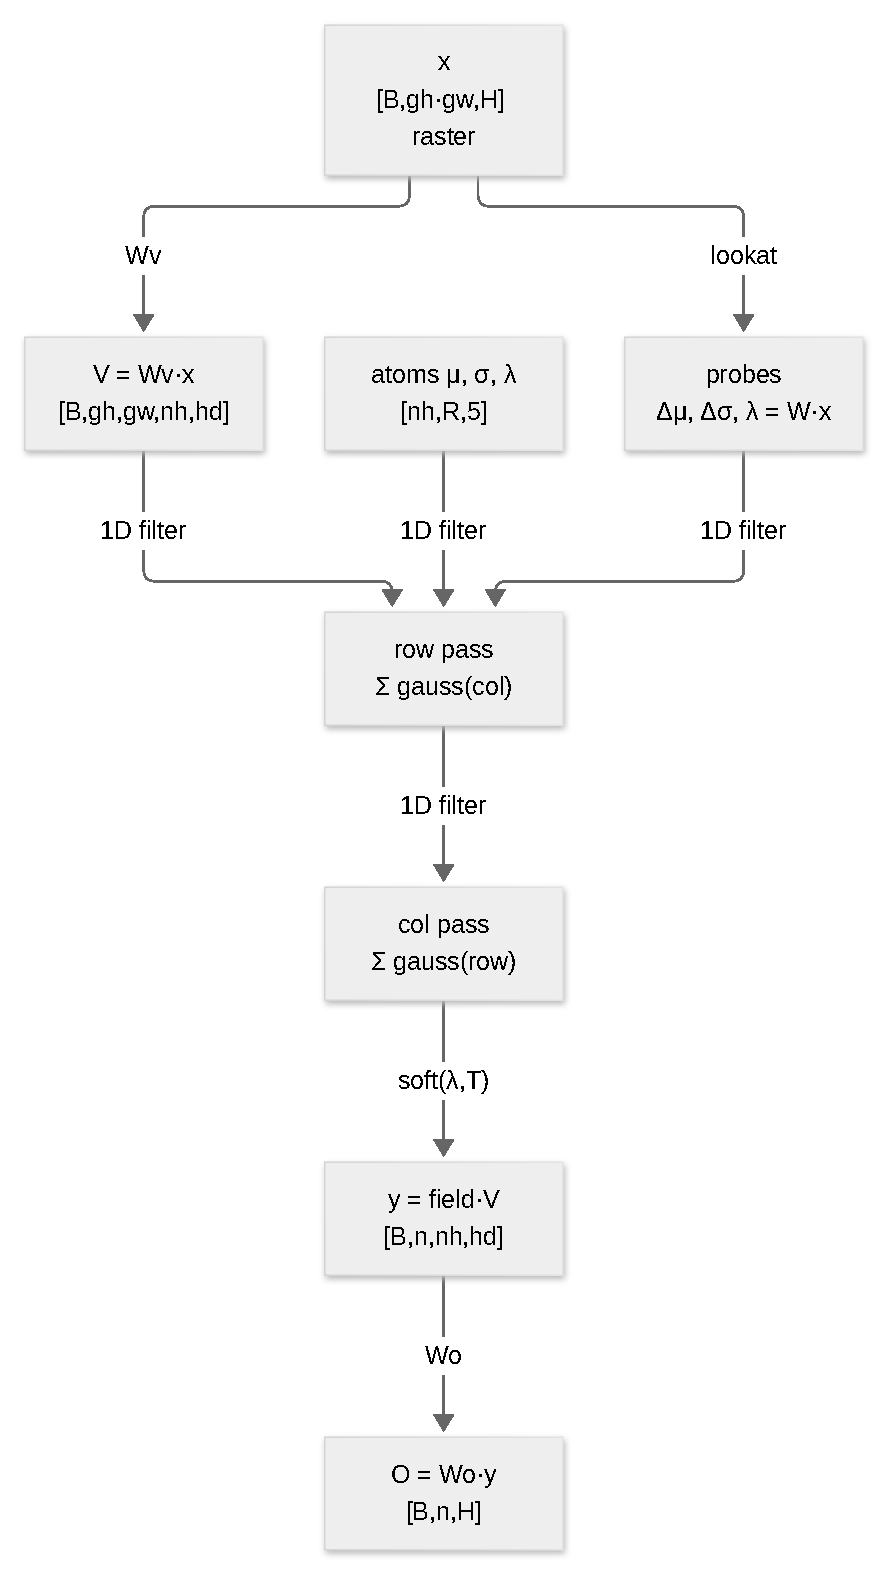
\includegraphics{figures/mixers/ssog.pdf}}
\caption{Dataflow of SSOG: values pass through separable row and column Gaussian filter passes per atom, with optional content steering of the atom parameters.}
\label{fig:mixer-ssog}
\end{figure}
\subsection{Mathematical Formulation}
Let tokens be the row-major raster of a $G_h \times G_w$ grid. The attention weight from token $p$ to token $q$ is the softmax-tempered log-sum-exp of the atom log-weights evaluated at their displacement:
\[
A(p, q) = \operatorname{softmax}_q\!\left( \tfrac{1}{\tau}\, s(p, q) \right),
\qquad
s(p, q) = \operatorname{logsumexp}_r \big( \log \lambda_r + \log \mathcal{N}(p - q;\ \mu_r, \sigma_r) \big),
\]
where $\tau$ is a learnable temperature and $\mathcal{N}(\cdot\,;\mu_r, \sigma_r)$ is a 2D Gaussian with diagonal covariance. Since the 2D Gaussian factorises, the softmaxed field applies separably: per axis, $a_y[i, j] = \operatorname{softmax}_j(\log \mathcal{N}(\Delta y_{ij}; \mu_y, \sigma_y) / \tau)$ and analogously $a_x$, followed by
\[
Y = \sum_{r=1}^{R} \lambda_r\, \big( a_x^{(r)} \big( a_y^{(r)}\, V \big) \big),
\qquad V = x W_V,
\]
i.e.\ three einsum contractions per layer. With content steering (\texttt{lookat}) enabled, zero-initialised linear probes predict bounded per-token residuals on the field parameters behind cold-started softplus gates:
\[
\mu \leftarrow \mu_0 + s_\mu \cdot m \cdot \tanh(W_\mu x), \qquad
\sigma \leftarrow \sigma_0 \, e^{s_\sigma \tanh(W_\sigma x)}, \qquad
\lambda \leftarrow \operatorname{softmax}\big( \log \lambda_0 + s_\lambda \tanh(W_\lambda x) \big),
\]
with $m$ the maximum offset in grid cells and gate scales $s_\bullet = \operatorname{softplus}(\cdot)$ initialised at $-8$ ($\approx 3 \times 10^{-4}$), so the model begins as a frozen geometric field and learns how far to open each content tap. Widths are reparameterised as $\sigma = \operatorname{softplus}(\omega) + \epsilon + \sigma_{\text{floor}}$ to stay strictly positive.

\subsection{Algorithmic Pseudocode}
\begin{algorithmic}[1]
\State \textbf{Input:} hidden state $x \in \mathbb{R}^{B \times N \times d}$ as a $G_h \times G_w$ raster, atoms $\{\mu_r, \omega_r, \log \lambda_r\}_{r=1}^{R}$ per head, temperature $\tau$
\State $V \gets x W_V$ reshaped to $(B, G_h, G_w, H, d_h)$ \Comment{no Q/K projections}
\State $\sigma_r \gets \operatorname{softplus}(\omega_r) + \epsilon + \sigma_{\text{floor}}$ \Comment{positive widths}
\If{steering (lookat)}
    \State $\mu, \sigma, \lambda \gets$ bounded per-token residuals via zero-init probes and gates \Comment{content steers}
\EndIf
\State $a_y \gets \operatorname{softmax}\!\big(\log \mathcal{N}(\Delta y; \mu_y, \sigma_y) / \tau\big)$, \quad $a_x \gets$ analogously \Comment{1D kernels, one per atom}
\State $Y \gets \sum_r \lambda_r\, a_x^{(r)} \big( a_y^{(r)} V \big)$ \Comment{row pass, column pass, $\lambda$-mix: no $N \times N$}
\State \textbf{Output:} $\mathbf{Y} W_O$ reshaped to $(B, N, d)$
\end{algorithmic}

\subsection{Key Characteristics}
\begin{itemize}[leftmargin=*]
    \item \textbf{Training complexity}: $\mathcal{O}(R \cdot N \sqrt{N} \cdot d)$ for fixed $R$ atoms---near-linear by geometry alone, not by kernel approximation.
    \item \textbf{Inference complexity}: same per-forward cost; encoder-only (the separable field has no causal formulation), so there are no KV-cache semantics.
    \item \textbf{Trainable}: atoms $\{\mu, \omega, \log\lambda\}$, temperature, and the steering probes are fully differentiable; cold-started gates open during optimisation.
    \item \textbf{Strengths}: strong geometric prior (+17 pts over SDPA on small data at matched recipe; beats SDPA on ImageNet-1k at 3M and 12M params with $\sim$20\% fewer parameters and $\sim$30\% fewer FLOPs); inherently interpretable (each head is a few plottable blobs---early layers become convolutions in disguise, middle layers strip detectors, late layers go global); the field lives on coordinates, granting zero-shot resolution transfer.
    \item \textbf{Limitations}: encoder-only; requires a fixed $G_h \times G_w$ row-major raster (ViT needs \texttt{cls\_token=false}; sequences need an explicit $1 \times L$ grid); the per-query steering kernels add a memory term; language results are unproven---content scoring is likely load-bearing there.
\end{itemize}

\section{Fast-Weight Attention for Continual Learning}
\label{sec:annex-fast-weight}

This annex covers the Falcon family \citep{zhang_falcon_2026}, a fast-weight attention framework that treats the recurrent fast-weight state transition as an \textbf{online continual-learning rule} under \emph{read-after-write} (RAW) autoregressive semantics. The framework's central observation is one of temporal alignment: for the prefix-prediction objective, the local fast-memory example revealed at step $t$ is the \textbf{prefix-aligned pair} $(x_t, y_t) = (\phi(k_{t-1}),\, v_t)$ --- one step shifted relative to the same-step association $(\phi(k_t), v_t)$ used by DeltaNet and standard linear attention. The same-step pairing remains causal, but it optimizes a different internal objective. The framework derives \textbf{normalized first-order updates} for two objectives (squared-error regression and negative inner product) and three step-size structures (scalar, per-column, sliding window), giving six variants: Falcon-1/2/3 (regression family) and Falcon-1A/2A/3A (inner-product family). All six are implemented in the codebase under \texttt{model.attention.falcon} with a shared configuration block, each providing both a recurrent reference scan and an SSD-style chunk-parallel kernel.

\subsection{Preliminaries: Alignment, Normalization, and Stability}

\paragraph{Read-after-write semantics.} With feature maps $\phi(k_t)$ (QK-RMSNorm by default, $\ell_2$ norm optional), the prefix-aligned stream sets $x_t = \phi(k_{t-1})$ for $t \ge 2$ with boundary sentinel $x_1 = 0$; the readout is $o_t = S_t^\top \phi(q_t)$. The write at step $t$ therefore updates the memory \emph{before} the query at step $t+1$ reads it, so no token's key ever associates with its own value.

\paragraph{Normalized first-order step sizes.} A gradient step on the local objective $\ell_t(S)$ with the objective-matched denominator gives
\[
\eta_t = \frac{\beta_t}{\text{statistic}_t + \lambda_t + \varepsilon}, \qquad \beta_t \in (0, 2),
\]
where the statistic is the squared key energy $\|x_t\|^2$ (Falcon-1/1A/2/2A), the window spectral statistic $\mu_t^{(B)} = \lambda_{\max}(X^\top X)/B_t$ (Falcon-3), or the window mean energy $\bar{E}_t^{(B)}$ (Falcon-3A). Objective-matched normalization guarantees per-step descent and removes the scale sensitivity of fixed learning rates. The \textbf{plasticity} gain $\beta_t$, the \textbf{forgetting} ridge $\lambda_t$, the temporal \textbf{alignment}, and the rehearsal window $B$ are thereby four previously entangled knobs, separated.

\paragraph{Positive-decay renormalization.} When $\lambda_t > 0$, the per-step shrinkage $\alpha_t = \min(\eta_t \lambda_t,\, 1 - \varepsilon_\gamma)$ must be applied stably. The implementation clamps $\alpha_t$ strictly below $1$, computes chunk-local log-prefixes in fp32 via $\log(1 - \alpha_t)$ and cumulative sums, rescales the drivers to the no-decay domain ($\tilde{\eta}_t = \eta_t / \gamma_t$, $\tilde{v}_t = v_t / c_{t-1}$ with $c_{t-1} = \prod_{r \le t-1} \gamma_r$), and rescales outputs and the emitted state back by the accumulated $\delta$. Boundary sentinels are $(\alpha_1, \gamma_1) = (0, 1)$ and $\eta_1 = 0$, so the first step is a pure read.

\subsection{The Regression Family (Falcon-1/2/3)}

The squared-error objective on the shifted pair is
\[
\ell_t(S) = \tfrac{1}{2}\|v_t - S^\top x_t\|^2 + \tfrac{\lambda_t}{2}\|S\|_F^2,
\qquad
\nabla_S \ell_t = x_t (S^\top x_t - v_t)^\top + \lambda_t S,
\]
which is $L_t$-smooth with $L_t = \|x_t\|^2 + \lambda_t$.

\subsubsection{Falcon-1: Scalar NLMS Regression}

\begin{figure}[H]
\centering
\fitfigure{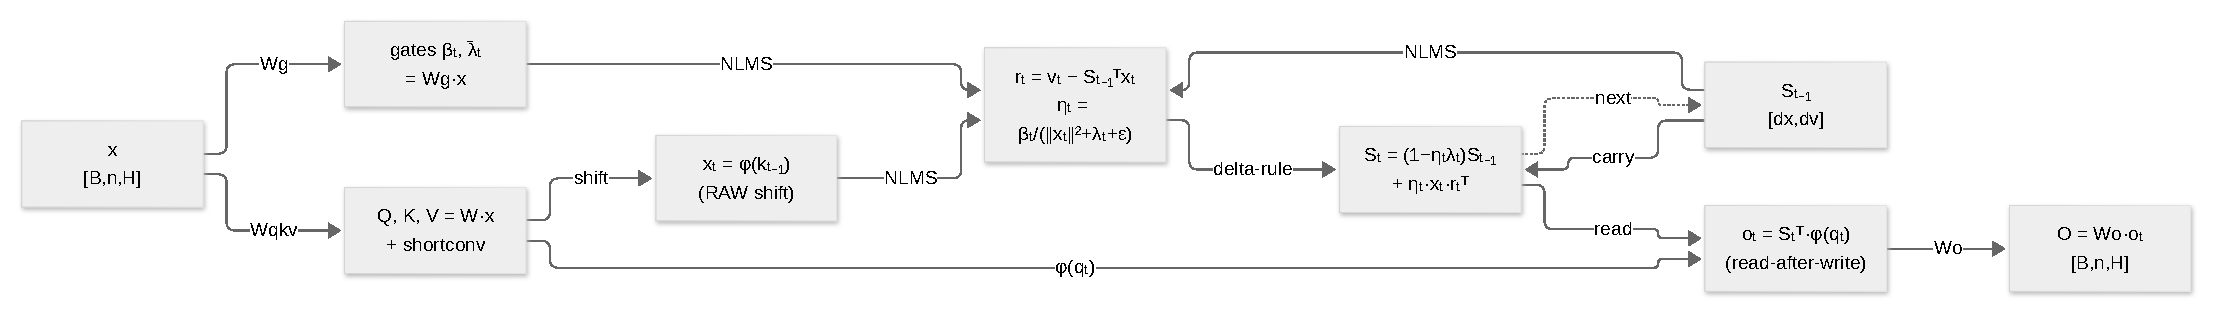
\includegraphics{figures/mixers/falcon1.pdf}}
\caption{Dataflow of Falcon-1: the prefix-aligned key/value pair drives a scalar NLMS delta-rule update of the fast-weight state.}
\label{fig:mixer-falcon1}
\end{figure}

The scalar delta-rule variant --- the classical NLMS recursion of adaptive filtering upgraded with the shifted write stream and an explicit ridge:
\[
S_t = (1 - \eta_t \lambda_t)\, S_{t-1} + \eta_t\, x_t \big(v_t - S_{t-1}^\top x_t\big)^\top,
\qquad
o_t = S_t^\top \phi(q_t).
\]
With $\varepsilon = 0$, $\lambda_t = 0$ and the unshifted assignment $x_t = \phi(k_t)$ this recovers DeltaNet exactly. The eigenstructure of the transition $A_t = \gamma_t I - \eta_t x_t x_t^\top$ (with $\gamma_t = 1 - \eta_t\lambda_t$) shows that the write direction contracts by $1 - \beta_t$ while the orthogonal subspace carries $\gamma_t$: $\beta_t > 1$ yields a stable sign-flip along the write direction, useful for state tracking. The chunk-parallel form uses the WY representation $\prod_s (I - \eta_s x_s x_s^\top) = I - U T U^\top$ with a single-residual unit-lower-triangular solve $L = \operatorname{tril}(G, -1) + I$ where $G = X^\top X$ (Algorithm~8 of the paper), after the positive-decay renormalization.

\subsubsection{Falcon-2: Per-Column NLMS Regression}

\begin{figure}[H]
\centering
\fitfigure{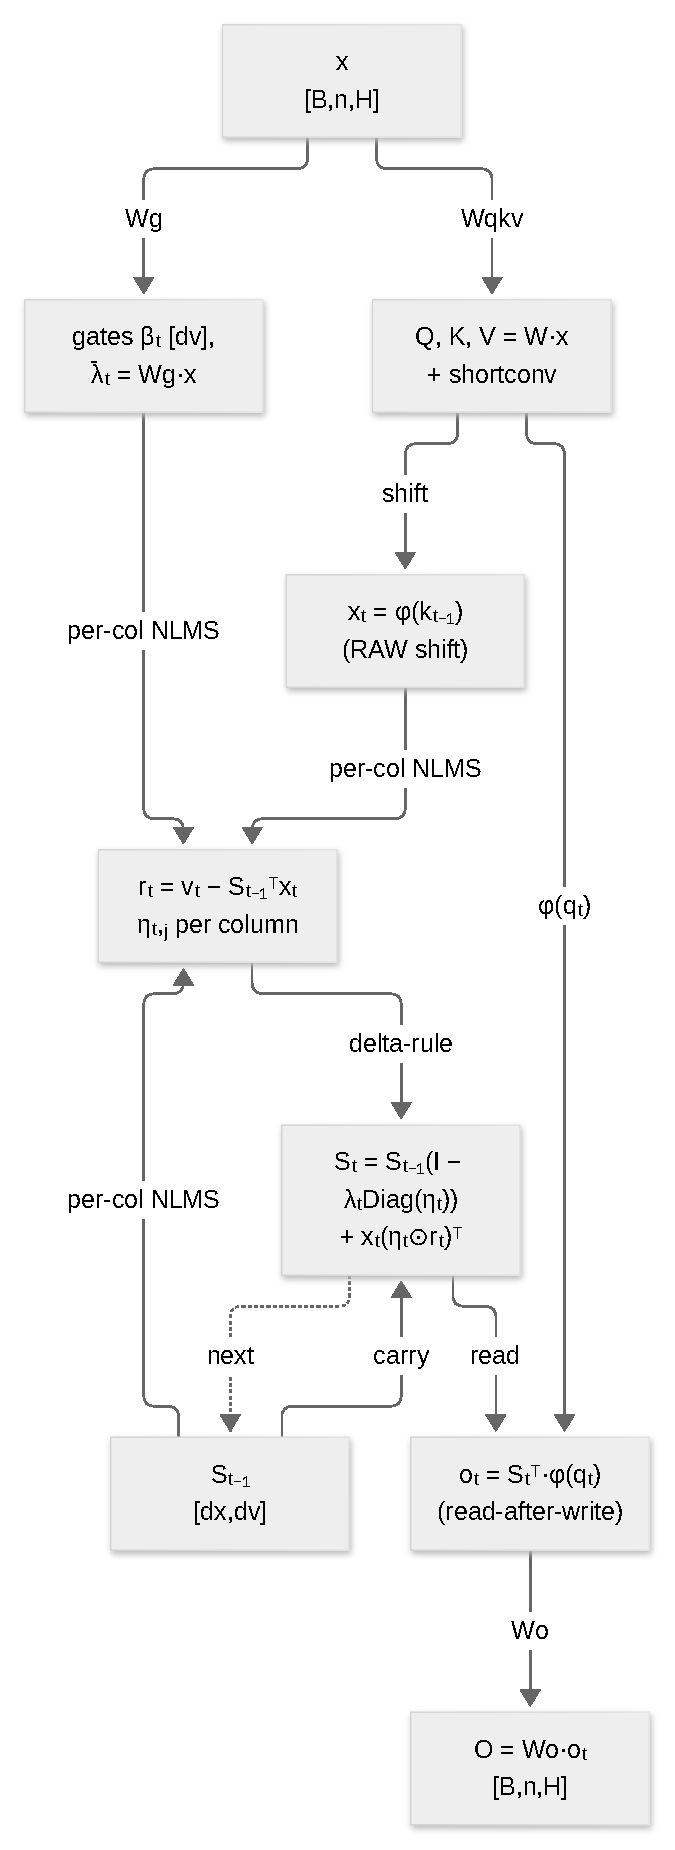
\includegraphics{figures/mixers/falcon2.pdf}}
\caption{Dataflow of Falcon-2: per-column NLMS step sizes update the fast-weight state channel by channel.}
\label{fig:mixer-falcon2}
\end{figure}

The ridge loss decomposes across value coordinates, so each value channel $j$ receives its own step size while sharing the NLMS normalizer:
\[
\eta_{j,t} = \frac{\beta_{j,t}}{\|x_t\|^2 + \lambda_t + \varepsilon},
\qquad
S_t = S_{t-1}\big(I - \lambda_t \operatorname{Diag}(\boldsymbol{\eta}_t)\big) + x_t \big(\boldsymbol{\eta}_t \odot \mathbf{r}_t\big)^\top .
\]
The chunk-parallel kernel forms the shared key Gram $G = X^\top X$ and solves the batch of per-channel unit-lower-triangular systems $L_j = I + \operatorname{tril}\big(G \odot (\Sigma_j \Sigma_j^\top), -1\big)$ with $\Sigma = \sqrt{\tilde{\boldsymbol{\eta}}}$ (Algorithm~1). Defined but not separately benchmarked in the paper.

\subsubsection{Falcon-3: Sliding-Window Minibatch Regression}

\begin{figure}[H]
\centering
\fitfigure{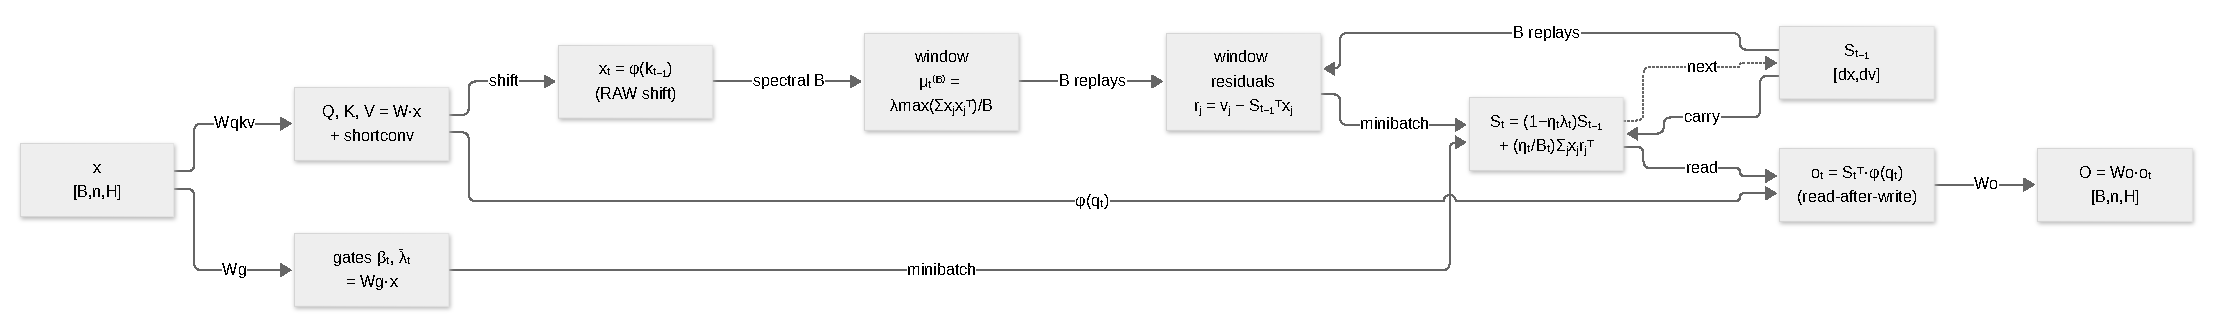
\includegraphics{figures/mixers/falcon3.pdf}}
\caption{Dataflow of Falcon-3: a sliding window of prefix-aligned pairs provides the spectral statistic and the minibatch write.}
\label{fig:mixer-falcon3}
\end{figure}

Bounded rehearsal: each step regresses the fast memory on the last $B_t \le B$ prefix-aligned pairs, with \emph{all window residuals evaluated at the pre-update state} $S_{t-1}$:
\[
\mu_t = \frac{\lambda_{\max}\big(X_{\mathcal{I}_t}^\top X_{\mathcal{I}_t}\big)}{B_t},
\qquad
\eta_t = \frac{\beta_t}{\mu_t + \lambda_t + \varepsilon},
\qquad
S_t = (1 - \eta_t \lambda_t)\, S_{t-1} + \frac{\eta_t}{B_t} \sum_{j \in \mathcal{I}_t} x_j \big(v_j - S_{t-1}^\top x_j\big)^\top ,
\]
with $\mathcal{I}_t = \{\max(2, t - B + 1), \dots, t\}$. Window-averaging keeps the update magnitude invariant to $B$: each pair is replayed in exactly $B$ consecutive updates at weight $1/B$, so its cumulative injection is $\eta$-independent of $B$. The state alone is \emph{not} Markov: exact continuation requires a FIFO tail of the last $B - 1$ pairs, and the chunk kernels gather an extended slice with $|\mathcal{J}| \le C + B - 1$. The chunk-parallel form is a rank-$B$ affine recurrence solved by block forward substitution over the (time $\times$ rank) extended index space, with same-time rank components uncoupled (Algorithm~3).

\subsection{The Inner-Product Family (Falcon-1A/2A/3A)}

The negative inner-product objective
\[
\ell_t^{\mathrm{ip}}(S) = -\langle S^\top x_t,\, v_t \rangle + \tfrac{\lambda_t}{2}\|S\|_F^2
\qquad \Rightarrow \qquad
\nabla_S \ell_t^{\mathrm{ip}} = -x_t v_t^\top + \lambda_t S
\]
yields purely additive (Hebbian) writes with energy-normalized gains.

\subsubsection{Falcon-1A and Falcon-2A}

\begin{figure}[H]
\centering
\fitfigure{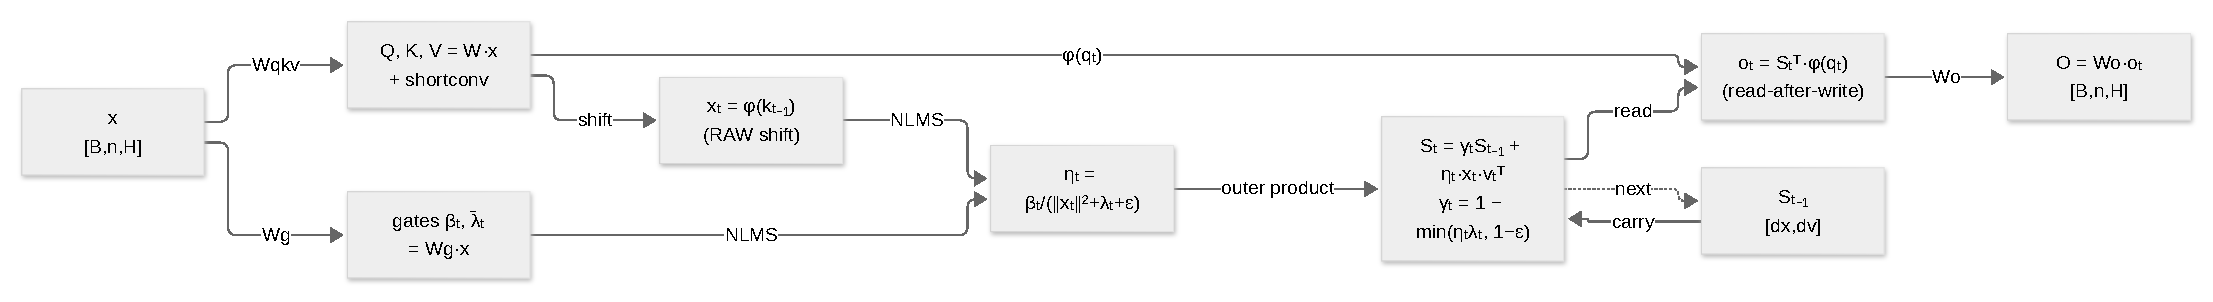
\includegraphics{figures/mixers/falcon1a.pdf}}
\caption{Dataflow of Falcon-1A: an energy-normalized additive (Hebbian) write with a derived decay.}
\label{fig:mixer-falcon1a}
\end{figure}

\begin{figure}[H]
\centering
\fitfigure{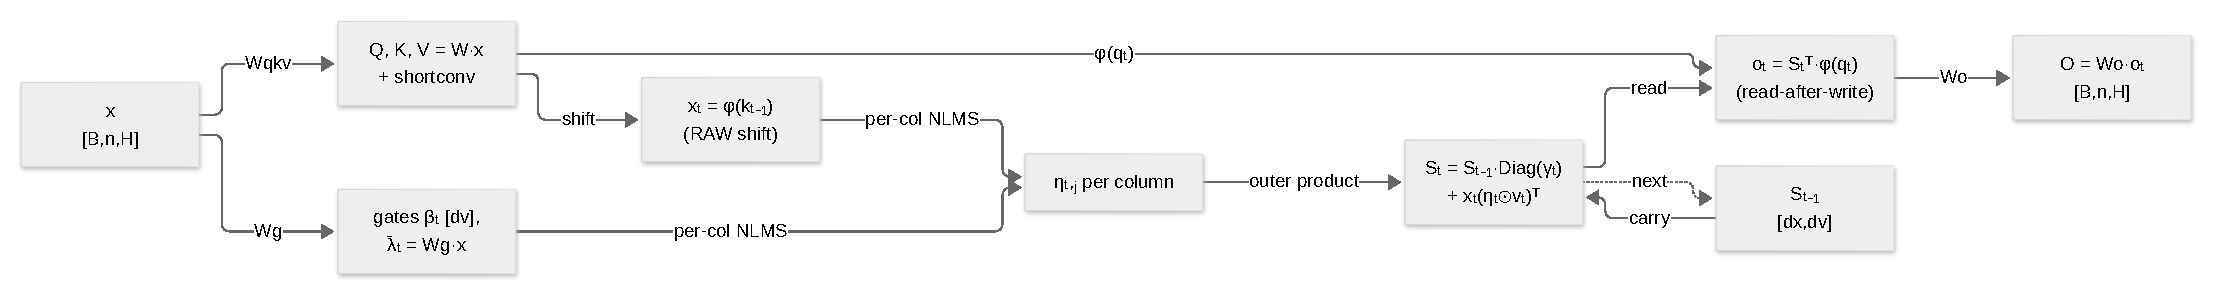
\includegraphics{figures/mixers/falcon2a.pdf}}
\caption{Dataflow of Falcon-2A: per-column additive writes with a per-channel decay.}
\label{fig:mixer-falcon2a}
\end{figure}

\[
\text{Falcon-1A:}\quad S_t = \gamma_t S_{t-1} + \eta_t\, x_t v_t^\top,
\quad \gamma_t = 1 - \min(\eta_t \lambda_t,\, 1 - \varepsilon_\gamma);
\qquad
\text{Falcon-2A:}\quad S_t = S_{t-1}\operatorname{Diag}(\boldsymbol{\gamma}_t) + x_t (\boldsymbol{\eta}_t \odot v_t)^\top .
\]
With $\lambda_t = 0$ and the unshifted assignment this is exactly standard linear attention / Mamba-2 accumulation; the shifted stream makes it the one-step-shifted next-latent variant. The A-family's denominator is not required by curvature (the objective is linear) --- it retains the energy-normalized write as a magnitude stabilizer. The chunk-parallel form is decay-mask linear attention with $M_{t,i} = \eta_i \prod_{r=i+1}^{t} \gamma_r$ (per-channel masks for Falcon-2A).

\subsubsection{Falcon-3A: Sliding-Window Inner-Product}

\begin{figure}[H]
\centering
\fitfigure{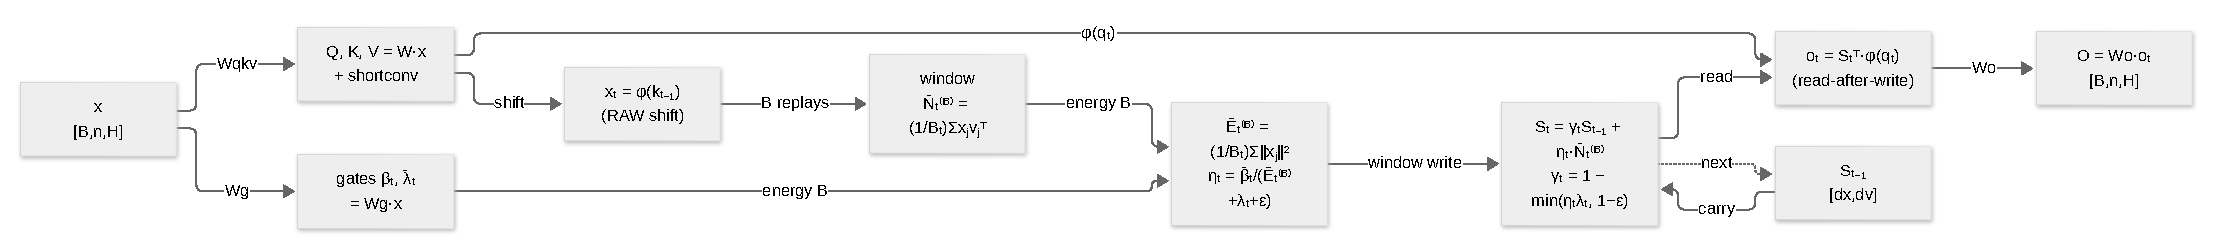
\includegraphics{figures/mixers/falcon3a.pdf}}
\caption{Dataflow of Falcon-3A: a sliding-window mean-energy statistic normalizes the additive window write.}
\label{fig:mixer-falcon3a}
\end{figure}

The windowed additive variant --- the family's best length-extrapolation configuration:
\[
\bar{N}_t^{(B)} = \frac{1}{B_t} \sum_{j \in \mathcal{I}_t} x_j v_j^\top,
\qquad
\bar{E}_t^{(B)} = \frac{1}{B_t} \sum_{j \in \mathcal{I}_t} \|x_j\|^2,
\qquad
\eta_t = \frac{\beta_t}{\bar{E}_t^{(B)} + \lambda_t + \varepsilon},
\qquad
S_t = \gamma_t S_{t-1} + \eta_t\, \bar{N}_t^{(B)} .
\]
The window-banded decay mask factors as $M = D \cdot \operatorname{Diag}(\boldsymbol{\eta}) \cdot A$, where $A$ is the $B$-banded window operator and $D$ the causal decay kernel, evaluated over the extended slice (Algorithm~4).

\subsection{Configuration Interface}

All six variants share one nested block, \texttt{model.attention.falcon}, selected through the \texttt{layer\_pattern} entries \texttt{falcon1\_attn}, \texttt{falcon2\_attn}, \texttt{falcon3\_attn}, \texttt{falcon1a\_attn}, \texttt{falcon2a\_attn}, \texttt{falcon3a\_attn}:

\begin{table}[H]
\centering
\small
\begin{tabularx}{0.95\linewidth}{llX}
\toprule
\textbf{Key} & \textbf{Default} & \textbf{Description} \\
\midrule
\texttt{chunk\_size} & $64$ & Chunk size of the chunk-parallel kernels; \texttt{null} selects the recurrent reference scan \\
\texttt{qk\_norm} & \texttt{rms\_norm} & QK normalization (\texttt{rms\_norm} or \texttt{l2\_norm}); RMSNorm computed in fp32 \\
\texttt{beta\_mode} & \texttt{ctx\_eta} & Plasticity gate parameterization: \texttt{static}, \texttt{ctx\_beta} (content-conditioned gain), or \texttt{ctx\_eta} (content-conditioned normalized step) \\
\texttt{lambda\_mode} & \texttt{ctx} & Forgetting gate: \texttt{static} or \texttt{ctx} (scale-couples with the detached curvature statistic) \\
\texttt{beta} / \texttt{lambda} & $1.0$ / $0.0$ & Static gain and ridge (used when the corresponding mode is \texttt{static}) \\
\texttt{window} & $4$ & Sliding window $B$ (Falcon-3 / Falcon-3A only) \\
\texttt{short\_conv} / \texttt{conv\_kernel} & \texttt{true} / $4$ & Causal depth-wise short convolutions on the q/k/v projections \\
\texttt{eps} / \texttt{eps\_gamma} & $10^{-6}$ / $10^{-4}$ & Step-size stabilizer and positive-decay clamp floor \\
\bottomrule
\end{tabularx}
\caption{Shared Falcon configuration knobs (\texttt{model.attention.falcon}). Each variant additionally exposes a per-mixer positional-encoding opt-out \texttt{falcon\{1,2,3,1a,2a,3a\}\_attn\_use\_pe}, default \texttt{False} like other recurrent/decay mixers.}
\label{tab:falcon-knobs}
\end{table}

Implementation notes: the recurrent and chunk-parallel kernels are verified numerically equivalent (chunk $\equiv$ recurrent to $\le 3.6 \times 10^{-7}$ across all six variants, including decay, multi-chunk, and windowed paths); gradients flow through the fp32 triangular-solve islands (feature drivers take only $\sqrt{\tilde{\eta}}$ while value targets take $\sqrt{\tilde{\eta}}\, e^{-u_{t-1}}$, with the square root clamped at $10^{-12}$ for NaN-free backward at the $\eta = 0$ boundary); positive exponents are clamped at $80$.

\subsection{Published Results}

\begin{table}[H]
\centering
\small
\begin{tabularx}{0.95\linewidth}{Xcccc}
\toprule
\textbf{Model (124M, 49.2B FineWeb-Edu tokens)} & \textbf{WikiText ppl} & \textbf{LMB. ppl} & \textbf{FineEdu ppl} & \textbf{0-shot avg} \\
\midrule
Transformer (RoPE) & 33.25 & 47.43 & 17.38 & 48.16 \\
Mamba-2 & 34.53 & 48.74 & 17.70 & 48.80 \\
DeltaNet & 34.19 & 52.84 & 17.84 & 48.88 \\
Gated DeltaNet & 30.99 & 46.70 & 17.32 & 48.78 \\
Falcon-1A.3 & 34.02 & 49.84 & 17.40 & 48.95 \\
Falcon-1.3 & 33.00 & 48.70 & \textbf{17.10} & \textbf{49.18} \\
\bottomrule
\end{tabularx}
\caption{Language modeling results reported by \citet{zhang_falcon_2026} at 124M parameters. On variable-digit addition length extrapolation (33--48 digits), Falcon-3A.3 reaches \textbf{87.2\%} mean accuracy versus 65.8\% for a RoPE Transformer and 85.9\% for Falcon-1A.3: the inner-product family carries arithmetic, while the regression family carries perplexity.}
\label{tab:falcon-results}
\end{table}

\subsection{Relation to Prior Work}

\begin{itemize}[leftmargin=*]
    \item \textbf{DeltaNet}: the delta rule is the squared-error one-gradient-descent step with the same-step pairing; Falcon recovers it with the critical index shift plus objective-matched normalization and explicit $\lambda_t$ shrinkage.
    \item \textbf{Gated DeltaNet}: adds a free learned carry gate; Falcon \emph{derives} the carry $\gamma_t = 1 - \eta_t \lambda_t$ from the local objective and the normalized step-size parameterization instead of adding an independent gate, and defaults to QK-RMSNorm rather than $\ell_2$ normalization.
    \item \textbf{Linear attention / Mamba-2}: the additive numerator is one gradient step on the inner-product objective with the unshifted assignment; the chunkwise kernels reuse the SSD scheme.
    \item \textbf{TTT / Titans / ATLAS}: fast-weight updates as test-time training; Falcon-3 is a sliding-window specialization of the internal-objective view with strict next-latent alignment.
    \item \textbf{Adaptive filtering (LMS/NLMS/RLS)}: Falcon imports the stability and normalization principles of NLMS into fast-weight attention under strict causality.
\end{itemize}

\subsubsection{When to Use Each Variant}

\begin{enumerate}[leftmargin=*]
    \item \textbf{Falcon-1}: best language-modeling perplexity of the family (FineEdu 17.10, beating Gated DeltaNet 17.32); principled forgetting tied to the local objective.
    \item \textbf{Falcon-2}: finer-grained plasticity than Falcon-1 at the cost of heavier per-channel chunk kernels; unbenchmarked in the paper.
    \item \textbf{Falcon-3}: controlled rehearsal horizon with exact window statistics; most complex kernel.
    \item \textbf{Falcon-1A}: simple and stable additive variant; second-best length extrapolation (85.9\%).
    \item \textbf{Falcon-2A}: channel-wise forgetting granularity; unbenchmarked.
    \item \textbf{Falcon-3A}: best length extrapolation of the paper (87.2\% on 33--48-digit addition); carries arithmetic tasks.
\end{enumerate}

\end{document}
